% Options for packages loaded elsewhere
\PassOptionsToPackage{unicode}{hyperref}
\PassOptionsToPackage{hyphens}{url}
%
\documentclass[
]{book}
\usepackage{lmodern}
\usepackage{amssymb,amsmath}
\usepackage{ifxetex,ifluatex}
\ifnum 0\ifxetex 1\fi\ifluatex 1\fi=0 % if pdftex
  \usepackage[T1]{fontenc}
  \usepackage[utf8]{inputenc}
  \usepackage{textcomp} % provide euro and other symbols
\else % if luatex or xetex
  \usepackage{unicode-math}
  \defaultfontfeatures{Scale=MatchLowercase}
  \defaultfontfeatures[\rmfamily]{Ligatures=TeX,Scale=1}
\fi
% Use upquote if available, for straight quotes in verbatim environments
\IfFileExists{upquote.sty}{\usepackage{upquote}}{}
\IfFileExists{microtype.sty}{% use microtype if available
  \usepackage[]{microtype}
  \UseMicrotypeSet[protrusion]{basicmath} % disable protrusion for tt fonts
}{}
\makeatletter
\@ifundefined{KOMAClassName}{% if non-KOMA class
  \IfFileExists{parskip.sty}{%
    \usepackage{parskip}
  }{% else
    \setlength{\parindent}{0pt}
    \setlength{\parskip}{6pt plus 2pt minus 1pt}}
}{% if KOMA class
  \KOMAoptions{parskip=half}}
\makeatother
\usepackage{xcolor}
\IfFileExists{xurl.sty}{\usepackage{xurl}}{} % add URL line breaks if available
\IfFileExists{bookmark.sty}{\usepackage{bookmark}}{\usepackage{hyperref}}
\hypersetup{
  pdftitle={Uso do sistema R para análise de dados},
  hidelinks,
  pdfcreator={LaTeX via pandoc}}
\urlstyle{same} % disable monospaced font for URLs
\usepackage{color}
\usepackage{fancyvrb}
\newcommand{\VerbBar}{|}
\newcommand{\VERB}{\Verb[commandchars=\\\{\}]}
\DefineVerbatimEnvironment{Highlighting}{Verbatim}{commandchars=\\\{\}}
% Add ',fontsize=\small' for more characters per line
\usepackage{framed}
\definecolor{shadecolor}{RGB}{248,248,248}
\newenvironment{Shaded}{\begin{snugshade}}{\end{snugshade}}
\newcommand{\AlertTok}[1]{\textcolor[rgb]{0.94,0.16,0.16}{#1}}
\newcommand{\AnnotationTok}[1]{\textcolor[rgb]{0.56,0.35,0.01}{\textbf{\textit{#1}}}}
\newcommand{\AttributeTok}[1]{\textcolor[rgb]{0.77,0.63,0.00}{#1}}
\newcommand{\BaseNTok}[1]{\textcolor[rgb]{0.00,0.00,0.81}{#1}}
\newcommand{\BuiltInTok}[1]{#1}
\newcommand{\CharTok}[1]{\textcolor[rgb]{0.31,0.60,0.02}{#1}}
\newcommand{\CommentTok}[1]{\textcolor[rgb]{0.56,0.35,0.01}{\textit{#1}}}
\newcommand{\CommentVarTok}[1]{\textcolor[rgb]{0.56,0.35,0.01}{\textbf{\textit{#1}}}}
\newcommand{\ConstantTok}[1]{\textcolor[rgb]{0.00,0.00,0.00}{#1}}
\newcommand{\ControlFlowTok}[1]{\textcolor[rgb]{0.13,0.29,0.53}{\textbf{#1}}}
\newcommand{\DataTypeTok}[1]{\textcolor[rgb]{0.13,0.29,0.53}{#1}}
\newcommand{\DecValTok}[1]{\textcolor[rgb]{0.00,0.00,0.81}{#1}}
\newcommand{\DocumentationTok}[1]{\textcolor[rgb]{0.56,0.35,0.01}{\textbf{\textit{#1}}}}
\newcommand{\ErrorTok}[1]{\textcolor[rgb]{0.64,0.00,0.00}{\textbf{#1}}}
\newcommand{\ExtensionTok}[1]{#1}
\newcommand{\FloatTok}[1]{\textcolor[rgb]{0.00,0.00,0.81}{#1}}
\newcommand{\FunctionTok}[1]{\textcolor[rgb]{0.00,0.00,0.00}{#1}}
\newcommand{\ImportTok}[1]{#1}
\newcommand{\InformationTok}[1]{\textcolor[rgb]{0.56,0.35,0.01}{\textbf{\textit{#1}}}}
\newcommand{\KeywordTok}[1]{\textcolor[rgb]{0.13,0.29,0.53}{\textbf{#1}}}
\newcommand{\NormalTok}[1]{#1}
\newcommand{\OperatorTok}[1]{\textcolor[rgb]{0.81,0.36,0.00}{\textbf{#1}}}
\newcommand{\OtherTok}[1]{\textcolor[rgb]{0.56,0.35,0.01}{#1}}
\newcommand{\PreprocessorTok}[1]{\textcolor[rgb]{0.56,0.35,0.01}{\textit{#1}}}
\newcommand{\RegionMarkerTok}[1]{#1}
\newcommand{\SpecialCharTok}[1]{\textcolor[rgb]{0.00,0.00,0.00}{#1}}
\newcommand{\SpecialStringTok}[1]{\textcolor[rgb]{0.31,0.60,0.02}{#1}}
\newcommand{\StringTok}[1]{\textcolor[rgb]{0.31,0.60,0.02}{#1}}
\newcommand{\VariableTok}[1]{\textcolor[rgb]{0.00,0.00,0.00}{#1}}
\newcommand{\VerbatimStringTok}[1]{\textcolor[rgb]{0.31,0.60,0.02}{#1}}
\newcommand{\WarningTok}[1]{\textcolor[rgb]{0.56,0.35,0.01}{\textbf{\textit{#1}}}}
\usepackage{longtable,booktabs}
% Correct order of tables after \paragraph or \subparagraph
\usepackage{etoolbox}
\makeatletter
\patchcmd\longtable{\par}{\if@noskipsec\mbox{}\fi\par}{}{}
\makeatother
% Allow footnotes in longtable head/foot
\IfFileExists{footnotehyper.sty}{\usepackage{footnotehyper}}{\usepackage{footnote}}
\makesavenoteenv{longtable}
\usepackage{graphicx,grffile}
\makeatletter
\def\maxwidth{\ifdim\Gin@nat@width>\linewidth\linewidth\else\Gin@nat@width\fi}
\def\maxheight{\ifdim\Gin@nat@height>\textheight\textheight\else\Gin@nat@height\fi}
\makeatother
% Scale images if necessary, so that they will not overflow the page
% margins by default, and it is still possible to overwrite the defaults
% using explicit options in \includegraphics[width, height, ...]{}
\setkeys{Gin}{width=\maxwidth,height=\maxheight,keepaspectratio}
% Set default figure placement to htbp
\makeatletter
\def\fps@figure{htbp}
\makeatother
\setlength{\emergencystretch}{3em} % prevent overfull lines
\providecommand{\tightlist}{%
  \setlength{\itemsep}{0pt}\setlength{\parskip}{0pt}}
\setcounter{secnumdepth}{5}
\usepackage{booktabs}
\usepackage[]{natbib}
\bibliographystyle{apalike}

\title{Uso do sistema R para análise de dados}
\author{}
\date{\vspace{-2.5em}2020-04-29}

\begin{document}
\maketitle

{
\setcounter{tocdepth}{1}
\tableofcontents
}
\hypertarget{pruxe9-requisitos}{%
\chapter{Pré requisitos}\label{pruxe9-requisitos}}

Material em construção.

Este material, em forma de notas de aula, foi escrito para a disciplina do Mestrado em Engenharia Agrícola, intitulado Uso do sistema R para análise de dados, no primeiro semestre de 2018.
Estas notas de aulas é uma coletânea de apostilas, livros, sites, forum e cursos voltando ao sistema R. Foi utilizado desses materiais sua estrutura didática e rotinas que foram adaptados para o perfil da disciplina.
O material consultado encontra-se referenciado no final de cada capitulo.

\hypertarget{r-buxe1sico}{%
\chapter{R Básico}\label{r-buxe1sico}}

Este primeio capítulo foi baseado no curso on-line denominada \emph{Code School Try R} e \emph{Datacamp}. Foram realizadas modificações utilizando-se de outros materiais que se encontram referenciado no final desse capítulo.

Primeiramente iremos abordar as expressões básicas do R.
Começaremos com comandos simples, como por exemplo, os comandos \textbf{números}, \textbf{strings} e valores \textbf{true/false}. Em seguida mostraremos como armazenar esses valores em variáveis e como transmitir as funções. Como obter ajuda sobre as funções e no final vamos carregar um arquivo.

\hypertarget{expressuxf5es}{%
\section{Expressões}\label{expressuxf5es}}

Vamos tentar algumas funções matemáticas simples. Digite o comando abaixo e aperte enter:

\begin{Shaded}
\begin{Highlighting}[]
\DecValTok{2}\OperatorTok{+}\DecValTok{8}
\end{Highlighting}
\end{Shaded}

\begin{verbatim}
## [1] 10
\end{verbatim}

Note que é impresso o resultado 10.

Digite a frase ``Engenharia Agrícola'':

\begin{Shaded}
\begin{Highlighting}[]
\StringTok{"Engenharia Agrícola"}
\end{Highlighting}
\end{Shaded}

\begin{verbatim}
## [1] "Engenharia Agrícola"
\end{verbatim}

Agora tente multiplicar 6x5 (* é o operador de multiplicação):

\begin{Shaded}
\begin{Highlighting}[]
\DecValTok{6}\OperatorTok{*}\DecValTok{5}
\end{Highlighting}
\end{Shaded}

\begin{verbatim}
## [1] 30
\end{verbatim}

\hypertarget{valores-booleanos}{%
\section{Valores Booleanos}\label{valores-booleanos}}

Algumas expressões retornam um ``valor lógico'': TRUE ou FALSE e/ou ``booleanos''.
Vamos tentar digitar uma expressões que nos dê um valor lógico:

\begin{Shaded}
\begin{Highlighting}[]
\DecValTok{7}\OperatorTok{<}\DecValTok{12}
\end{Highlighting}
\end{Shaded}

\begin{verbatim}
## [1] TRUE
\end{verbatim}

E outro valor lógico (sinal duplo de igualdade):

\begin{Shaded}
\begin{Highlighting}[]
\DecValTok{6}\OperatorTok{+}\DecValTok{5}\OperatorTok{==}\DecValTok{10}
\end{Highlighting}
\end{Shaded}

\begin{verbatim}
## [1] FALSE
\end{verbatim}

\textbf{T} e \textbf{F} são taquigrafia para TRUE e FALSE. Tente isso:

\begin{Shaded}
\begin{Highlighting}[]
\NormalTok{F}\OperatorTok{==}\OtherTok{FALSE}
\end{Highlighting}
\end{Shaded}

\begin{verbatim}
## [1] TRUE
\end{verbatim}

\hypertarget{variuxe1veis}{%
\section{Variáveis}\label{variuxe1veis}}

Você pode armazenar valores em uma variável para usar mais tarde.
Digite \textbf{x \textless- 28} para armazenar um valor em \textbf{x}:

\begin{Shaded}
\begin{Highlighting}[]
\NormalTok{x<-}\DecValTok{28}
\end{Highlighting}
\end{Shaded}

Tende dividr \textbf{x} por \textbf{4}( \textbf{/} é o operador da divisão):

\begin{Shaded}
\begin{Highlighting}[]
\NormalTok{x}\OperatorTok{/}\DecValTok{4}
\end{Highlighting}
\end{Shaded}

\begin{verbatim}
## [1] 7
\end{verbatim}

Você pode retribuir qualquer valor a uma variável a qualquer momento.
Tente atribuir ``Engenharia Agrícola''em x:

\begin{Shaded}
\begin{Highlighting}[]
\NormalTok{x <-}\StringTok{ "Engenharia Agrícola"}
\end{Highlighting}
\end{Shaded}

Tente imprimir o valor atual de x:

\begin{Shaded}
\begin{Highlighting}[]
\NormalTok{x}
\end{Highlighting}
\end{Shaded}

\begin{verbatim}
## [1] "Engenharia Agrícola"
\end{verbatim}

\hypertarget{funuxe7uxf5es}{%
\section{Funções}\label{funuxe7uxf5es}}

Você pode chamar uma \textbf{função} digitando seu nome, seguido de um ou mais argumentos para essa função entre parênteses.

Vamos tentar usar a função \texttt{sum()} para adicionar alguns números. Entrar com o comando:

\begin{Shaded}
\begin{Highlighting}[]
\KeywordTok{sum}\NormalTok{ (}\DecValTok{2}\NormalTok{, }\DecValTok{4}\NormalTok{, }\DecValTok{6}\NormalTok{)}
\end{Highlighting}
\end{Shaded}

\begin{verbatim}
## [1] 12
\end{verbatim}

Alguns argumentos têm nomes. Por exemplo, para repetir um valor 3 vezes você chamaria a função \texttt{rep} e forneceria seu argumento \textbf{times}:

\begin{Shaded}
\begin{Highlighting}[]
\KeywordTok{rep}\NormalTok{(}\StringTok{"Engenharia Agrícola"}\NormalTok{, }\DataTypeTok{times=}\DecValTok{3}\NormalTok{)}
\end{Highlighting}
\end{Shaded}

\begin{verbatim}
## [1] "Engenharia Agrícola" "Engenharia Agrícola" "Engenharia Agrícola"
\end{verbatim}

Tente chamar a função \texttt{sqrt} para obter a raiz quadrada de 16:

\begin{Shaded}
\begin{Highlighting}[]
\KeywordTok{sqrt}\NormalTok{(}\DecValTok{16}\NormalTok{)}
\end{Highlighting}
\end{Shaded}

\begin{verbatim}
## [1] 4
\end{verbatim}

\hypertarget{ajuda}{%
\section{Ajuda}\label{ajuda}}

A função \texttt{help\ ()} fornece ajuda para a função desejada. Tente exibir ajuda para a função \texttt{mean}:

\begin{Shaded}
\begin{Highlighting}[]
\KeywordTok{help}\NormalTok{ (mean)}
\end{Highlighting}
\end{Shaded}

\begin{verbatim}
## starting httpd help server ... done
\end{verbatim}

A função \texttt{example\ ()} traz exemplos de usos. Tente exibir exemplos para a função \texttt{min}:

\begin{Shaded}
\begin{Highlighting}[]
\KeywordTok{example}\NormalTok{(min)}
\end{Highlighting}
\end{Shaded}

\begin{verbatim}
## 
## min> require(stats); require(graphics)
## 
## min>  min(5:1, pi) #-> one number
## [1] 1
## 
## min> pmin(5:1, pi) #->  5  numbers
## [1] 3.141593 3.141593 3.000000 2.000000 1.000000
## 
## min> x <- sort(rnorm(100));  cH <- 1.35
## 
## min> pmin(cH, quantile(x)) # no names
## [1] -2.1022701 -0.8814625 -0.1372696  0.5362824  1.3500000
## 
## min> pmin(quantile(x), cH) # has names
##         0%        25%        50%        75%       100% 
## -2.1022701 -0.8814625 -0.1372696  0.5362824  1.3500000 
## 
## min> plot(x, pmin(cH, pmax(-cH, x)), type = "b", main =  "Huber's function")
\end{verbatim}

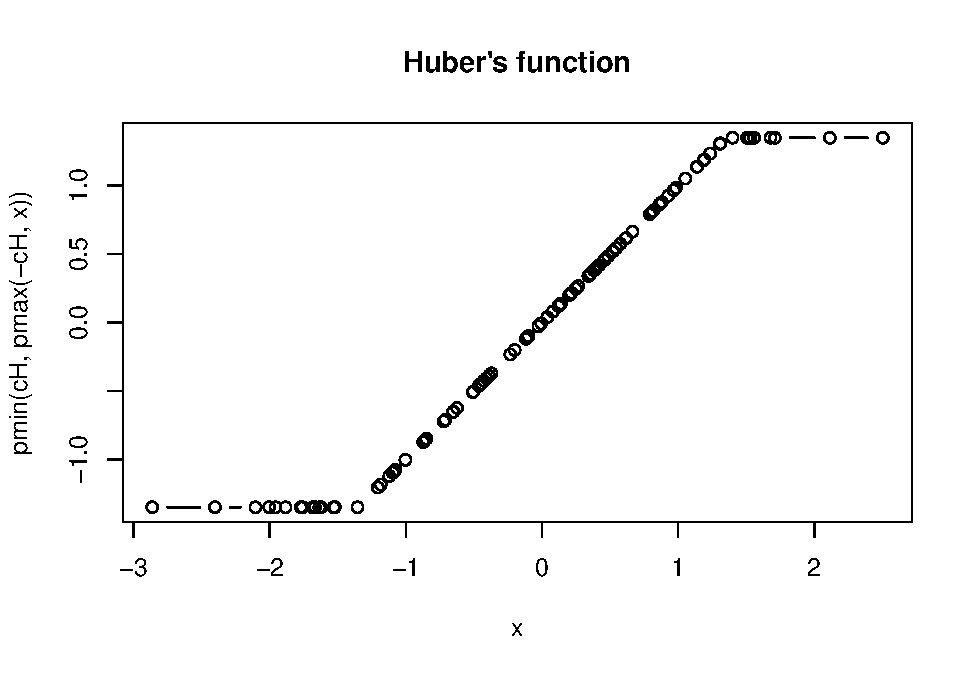
\includegraphics{TudodoR_files/figure-latex/unnamed-chunk-14-1.pdf}

\begin{verbatim}
## 
## min> cut01 <- function(x) pmax(pmin(x, 1), 0)
## 
## min> curve(      x^2 - 1/4, -1.4, 1.5, col = 2)
\end{verbatim}

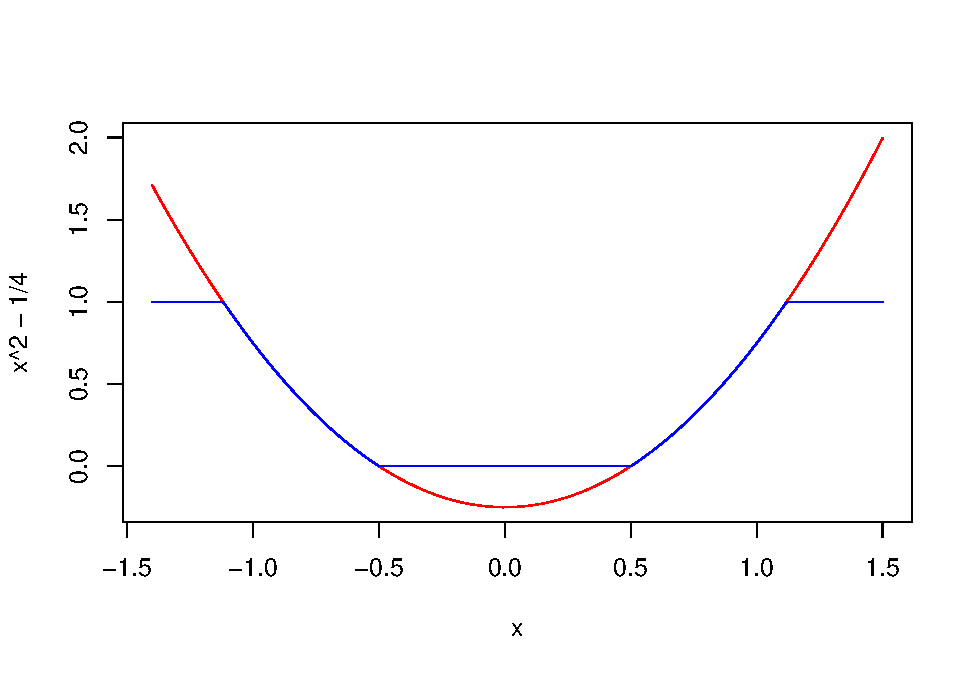
\includegraphics{TudodoR_files/figure-latex/unnamed-chunk-14-2.pdf}

\begin{verbatim}
## 
## min> curve(cut01(x^2 - 1/4), col = "blue", add = TRUE, n = 500)
## 
## min> ## pmax(), pmin() preserve attributes of *first* argument
## min> D <- diag(x = (3:1)/4) ; n0 <- numeric()
## 
## min> stopifnot(identical(D,  cut01(D) ),
## min+           identical(n0, cut01(n0)),
## min+           identical(n0, cut01(NULL)),
## min+           identical(n0, pmax(3:1, n0, 2)),
## min+           identical(n0, pmax(n0, 4)))
\end{verbatim}

\hypertarget{referuxeancia}{%
\section{Referência}\label{referuxeancia}}

MELO, M. P.; PETERNELI, L. A. \textbf{Conhecendo o R: Um visão mais que estatística}. Viçosa, MG: UFV, 2013. 222p.

\textbf{Prof.~Paulo Justiniando Ribeiro} \textgreater{}\url{http://www.leg.ufpr.br/~paulojus/}\textless{}

\textbf{Prof.~Adriano Azevedo Filho} \textgreater{}\url{http://rpubs.com/adriano/esalq2012inicial}\textless{}

\textbf{Prof.~Fernando de Pol Mayer} \textgreater{}\url{https://fernandomayer.github.io/ce083-2016-2/}\textless{}

\textbf{Site Interativo Datacamp} \textgreater{}\url{https://www.datacamp.com/}\textless{}

\hypertarget{estruturas-de-dados}{%
\chapter{Estruturas de Dados}\label{estruturas-de-dados}}

Este segundo capítulo foi baseado no curso on-line \emph{Code School Try R} e no livro \href{https://www.editoraufv.com.br/produto/conhecendo-o-r-uma-visao-mais-que-estatistica/1109294}{\textbf{Conhecendo o R: Um visão mais que estatística}}, modificações foram realizadas utilizando outros materiais que se encontram referenciados no final desse capítulo.

\hypertarget{vetor}{%
\section{Vetor}\label{vetor}}

Um vetor é simplesmente uma lista de valores.
A maneira mais simples de usar um vetor é usando o comando \texttt{c()}, que concatena elementos num mesmo objeto.
Exemplo:

\begin{Shaded}
\begin{Highlighting}[]
\NormalTok{x<-}\StringTok{ }\KeywordTok{c}\NormalTok{(}\DecValTok{2}\NormalTok{,}\DecValTok{3}\NormalTok{,}\DecValTok{5}\NormalTok{,}\DecValTok{7}\NormalTok{,}\DecValTok{11}\NormalTok{) }
\NormalTok{x}
\end{Highlighting}
\end{Shaded}

\begin{verbatim}
## [1]  2  3  5  7 11
\end{verbatim}

Os argumentos de \texttt{c()} podem ser tanto elementos únicos quanto outros objetos. Adicione três números no \textbf{vetor x}:

\begin{Shaded}
\begin{Highlighting}[]
\NormalTok{y<-}\StringTok{ }\KeywordTok{c}\NormalTok{(x,}\DecValTok{13}\NormalTok{,}\DecValTok{17}\NormalTok{,}\DecValTok{19}\NormalTok{)}
\NormalTok{y}
\end{Highlighting}
\end{Shaded}

\begin{verbatim}
## [1]  2  3  5  7 11 13 17 19
\end{verbatim}

\hypertarget{vetores-de-sequuxeancia}{%
\subsection{Vetores de Sequência}\label{vetores-de-sequuxeancia}}

Se você precisar de um vetor com uma sequência de números, você pode criá-lo com a notação \emph{start:end}. Vamos fazer um vetor com valores de 1 a 7:

\begin{Shaded}
\begin{Highlighting}[]
\DecValTok{1}\OperatorTok{:}\DecValTok{7}
\end{Highlighting}
\end{Shaded}

\begin{verbatim}
## [1] 1 2 3 4 5 6 7
\end{verbatim}

Uma maneira mais versátil de fazer sequências é chamar a função \texttt{seq}. Vamos fazer o mesmo com \texttt{seq\ ()}:

\begin{Shaded}
\begin{Highlighting}[]
\KeywordTok{seq}\NormalTok{(}\DecValTok{1}\OperatorTok{:}\DecValTok{7}\NormalTok{)}
\end{Highlighting}
\end{Shaded}

\begin{verbatim}
## [1] 1 2 3 4 5 6 7
\end{verbatim}

A função \texttt{seq} também permite que você use incrementos diferentes de 1. Experimente com as etapas de 0.5:

\begin{Shaded}
\begin{Highlighting}[]
\KeywordTok{seq}\NormalTok{(}\DecValTok{1}\NormalTok{,}\DecValTok{7}\NormalTok{,}\FloatTok{0.5}\NormalTok{)}
\end{Highlighting}
\end{Shaded}

\begin{verbatim}
##  [1] 1.0 1.5 2.0 2.5 3.0 3.5 4.0 4.5 5.0 5.5 6.0 6.5 7.0
\end{verbatim}

\begin{Shaded}
\begin{Highlighting}[]
\KeywordTok{seq}\NormalTok{(}\DecValTok{7}\NormalTok{,}\DecValTok{1}\NormalTok{,}\OperatorTok{-}\FloatTok{0.5}\NormalTok{) }
\end{Highlighting}
\end{Shaded}

\begin{verbatim}
##  [1] 7.0 6.5 6.0 5.5 5.0 4.5 4.0 3.5 3.0 2.5 2.0 1.5 1.0
\end{verbatim}

Todo objeto possui atributos intrínsecos, como tipo e tamanho. Com relação ao tipo, ele pode ser: \textbf{numérico}, \textbf{caractere}, \textbf{complexo} e \textbf{lógico}. Existem outros tipos, como por exemplo, funções ou expressões, porém esses não representam dados.
As funções \texttt{mode()} e \texttt{length()} mostram o tipo e tamanho de um objeto, respectivamente:

\begin{Shaded}
\begin{Highlighting}[]
\NormalTok{z<-}\KeywordTok{c}\NormalTok{(}\DecValTok{1}\NormalTok{,}\DecValTok{3}\NormalTok{,}\DecValTok{5}\NormalTok{,}\DecValTok{7}\NormalTok{,}\DecValTok{11}\NormalTok{) }
\KeywordTok{mode}\NormalTok{ (z)}
\end{Highlighting}
\end{Shaded}

\begin{verbatim}
## [1] "numeric"
\end{verbatim}

\begin{Shaded}
\begin{Highlighting}[]
\KeywordTok{length}\NormalTok{(z)}
\end{Highlighting}
\end{Shaded}

\begin{verbatim}
## [1] 5
\end{verbatim}

\begin{Shaded}
\begin{Highlighting}[]
\NormalTok{a <-}\StringTok{ "Angela"}
\NormalTok{b<-}\OtherTok{TRUE}\NormalTok{; }
\NormalTok{c<-8i }\CommentTok{#objetos com tipos diferentes}
\KeywordTok{mode}\NormalTok{(a); }
\end{Highlighting}
\end{Shaded}

\begin{verbatim}
## [1] "character"
\end{verbatim}

\begin{Shaded}
\begin{Highlighting}[]
\KeywordTok{mode}\NormalTok{(b); }
\end{Highlighting}
\end{Shaded}

\begin{verbatim}
## [1] "logical"
\end{verbatim}

\begin{Shaded}
\begin{Highlighting}[]
\KeywordTok{mode}\NormalTok{(c) }\CommentTok{#exibe os atributos "tipo" dos objetos }
\end{Highlighting}
\end{Shaded}

\begin{verbatim}
## [1] "complex"
\end{verbatim}

Se o vetor é muito longo e não ``cabe'' em uma linha, o R vai usar as linhas seguintes para continuar imprimindo o vetor:

\begin{Shaded}
\begin{Highlighting}[]
\NormalTok{longo<-}\DecValTok{100}\OperatorTok{:}\DecValTok{50} \CommentTok{#sequência decrescente de 100 a 50}
\NormalTok{longo }\CommentTok{#exibe o conteúdo do objeto }
\end{Highlighting}
\end{Shaded}

\begin{verbatim}
##  [1] 100  99  98  97  96  95  94  93  92  91  90  89  88  87  86  85  84  83  82
## [20]  81  80  79  78  77  76  75  74  73  72  71  70  69  68  67  66  65  64  63
## [39]  62  61  60  59  58  57  56  55  54  53  52  51  50
\end{verbatim}

Os números entre os colchetes não fazem parte do objeto e indicam a posição do vetor naquele ponto. Pode-se ver que {[}1{]} indica que o primeiro elemento do vetor estão naquela linha, e o {[}17{]} indica que a linha seguinte começa pelo décimo sétimo elemento do vetor e assim por diante.

Você pode recuperar um valor individual dentro de um vetor fornecendo seu índice numérico entre colchetes. Tente obter o valor 18:

\begin{Shaded}
\begin{Highlighting}[]
\NormalTok{longo[}\DecValTok{18}\NormalTok{]}
\end{Highlighting}
\end{Shaded}

\begin{verbatim}
## [1] 83
\end{verbatim}

Muitas línguagens de programação iniciam índices de matriz em 0, mas os índices vetoriais de R começam em 1. Obtenha o primeiro valor digitando:

\begin{Shaded}
\begin{Highlighting}[]
\NormalTok{longo[}\DecValTok{1}\NormalTok{]}
\end{Highlighting}
\end{Shaded}

\begin{verbatim}
## [1] 100
\end{verbatim}

Você pode atribuir novos valores dentro de um vetor existente. Tente mudar o terceiro valor \textbf{28}:

\begin{Shaded}
\begin{Highlighting}[]
\NormalTok{longo [}\DecValTok{3}\NormalTok{] <-}\StringTok{ }\DecValTok{28}
\end{Highlighting}
\end{Shaded}

Se você adicionar novos valores no final, o vetor aumentará para acomodá-los. Vamos adicionar um valor no final:

\begin{Shaded}
\begin{Highlighting}[]
\NormalTok{longo[}\DecValTok{101}\NormalTok{] <-}\StringTok{ }\DecValTok{83}
\end{Highlighting}
\end{Shaded}

Você pode usar um vetor entre os colchetes para acessar vários valores. Tente obter a primeira e a terceira palavra:

\begin{Shaded}
\begin{Highlighting}[]
\NormalTok{longo[}\KeywordTok{c}\NormalTok{(}\DecValTok{1}\NormalTok{,}\DecValTok{3}\NormalTok{)]}
\end{Highlighting}
\end{Shaded}

\begin{verbatim}
## [1] 100  28
\end{verbatim}

Isso significa que você pode recuperar intervalos de valores. Obter a segunda e a quarta palavra:

\begin{Shaded}
\begin{Highlighting}[]
\NormalTok{longo[}\DecValTok{2}\OperatorTok{:}\DecValTok{4}\NormalTok{]}
\end{Highlighting}
\end{Shaded}

\begin{verbatim}
## [1] 99 28 97
\end{verbatim}

Você também pode definir intervalos de valores. Apenas fornecendo os valores em um vetor. Adicione valores 5 a 7:

\begin{Shaded}
\begin{Highlighting}[]
\NormalTok{longo[}\DecValTok{5}\OperatorTok{:}\DecValTok{7}\NormalTok{] <-}\StringTok{ }\KeywordTok{c}\NormalTok{(}\DecValTok{42}\NormalTok{,}\DecValTok{52}\NormalTok{,}\DecValTok{75}\NormalTok{)}
\end{Highlighting}
\end{Shaded}

Agora tente acessar o oitavo valor do vetor:

\begin{Shaded}
\begin{Highlighting}[]
\NormalTok{longo[}\DecValTok{8}\NormalTok{]}
\end{Highlighting}
\end{Shaded}

\begin{verbatim}
## [1] 93
\end{verbatim}

\hypertarget{nomes-de-vetores}{%
\subsection{Nomes de vetores}\label{nomes-de-vetores}}

Para esse desafio, criaremos um vetor de 3 itens, e na sequência iremos armazená-lo na variável solo.
Você pode atribuir nomes aos elementos de um vetor passando um segundo vetor preenchido com os nomes com a função \texttt{names\ ()}, assim:

\begin{Shaded}
\begin{Highlighting}[]
\NormalTok{solo <-}\StringTok{ }\DecValTok{1}\OperatorTok{:}\DecValTok{3}
\KeywordTok{names}\NormalTok{(solo) <-}\StringTok{ }\KeywordTok{c}\NormalTok{(}\StringTok{"Argila"}\NormalTok{, }\StringTok{"Areia"}\NormalTok{,}\StringTok{"Silte"}\NormalTok{ )}
\NormalTok{solo}
\end{Highlighting}
\end{Shaded}

\begin{verbatim}
## Argila  Areia  Silte 
##      1      2      3
\end{verbatim}

Agora defina o valor atual para o \emph{silte} para um valor diferente usando o nome em vez da posição:

\begin{Shaded}
\begin{Highlighting}[]
\NormalTok{solo[}\StringTok{"Silte"}\NormalTok{]<-}\DecValTok{20}
\end{Highlighting}
\end{Shaded}

\hypertarget{plotando-um-vetor}{%
\subsection{Plotando um vetor}\label{plotando-um-vetor}}

A função \texttt{barplot\ ()} desenha um gráfico de barras com os valores de um vetor. Vamos criar um novo vetor e armazená-lo na variável chuva.

Agora tente passar o vetor para a função \texttt{barplot}:

\begin{Shaded}
\begin{Highlighting}[]
\NormalTok{chuva <-}\StringTok{ }\KeywordTok{c}\NormalTok{(}\DecValTok{20}\NormalTok{,}\DecValTok{50}\NormalTok{,}\DecValTok{85}\NormalTok{)}
\KeywordTok{barplot}\NormalTok{(chuva)}
\end{Highlighting}
\end{Shaded}

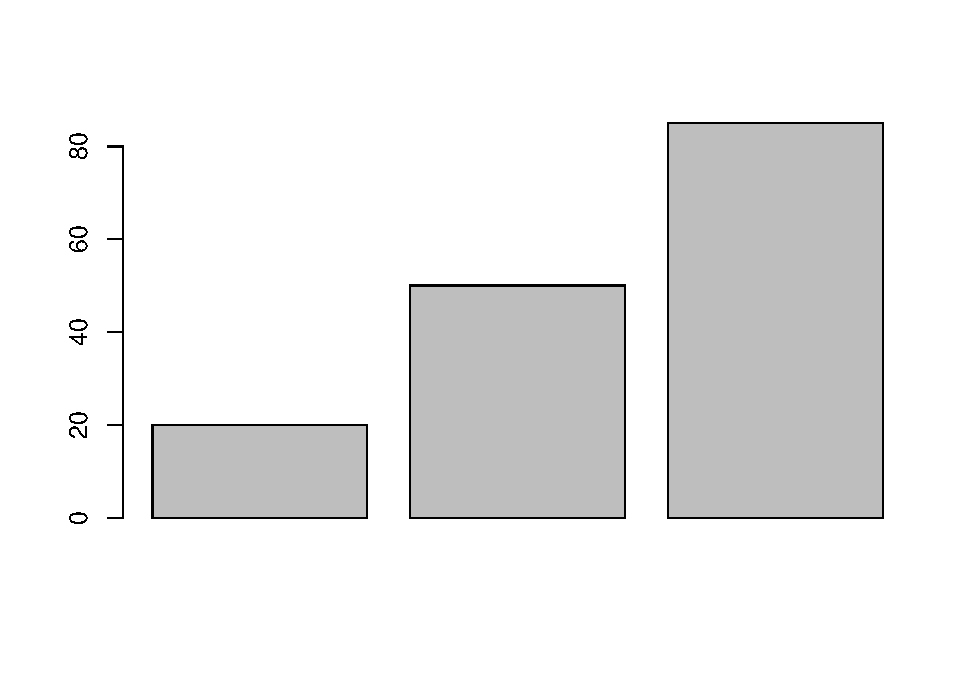
\includegraphics{TudodoR_files/figure-latex/unnamed-chunk-32-1.pdf}

Se você atribuir nomes aos valores do vetor, o R usará esses nomes como rótulos no gráfico da barra. Vamos usar a função \texttt{names\ ()} novamente:

\begin{Shaded}
\begin{Highlighting}[]
\KeywordTok{names}\NormalTok{(chuva)<-}\StringTok{ }\KeywordTok{c}\NormalTok{(}\StringTok{"Rondonópolis", "}\NormalTok{Maringá}\StringTok{", "}\NormalTok{Cruzeiro do Sul}\StringTok{")}
\end{Highlighting}
\end{Shaded}

Se você digitar \texttt{barplot\ (chuva)} com o vetor novamente, você verá os rótulos:

\begin{Shaded}
\begin{Highlighting}[]
\KeywordTok{barplot}\NormalTok{(chuva)}
\end{Highlighting}
\end{Shaded}

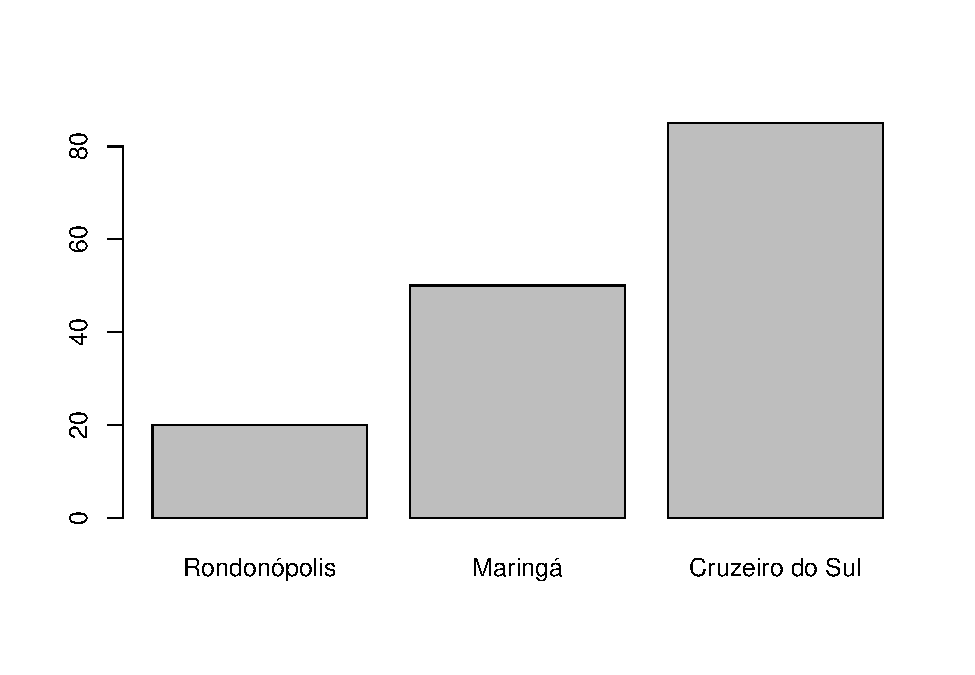
\includegraphics{TudodoR_files/figure-latex/unnamed-chunk-34-1.pdf}

Tente chamar \texttt{barplot} em um vetor de números inteiros que variam de 1 a 100:

\begin{Shaded}
\begin{Highlighting}[]
\KeywordTok{barplot}\NormalTok{(}\DecValTok{1}\OperatorTok{:}\DecValTok{100}\NormalTok{)}
\end{Highlighting}
\end{Shaded}

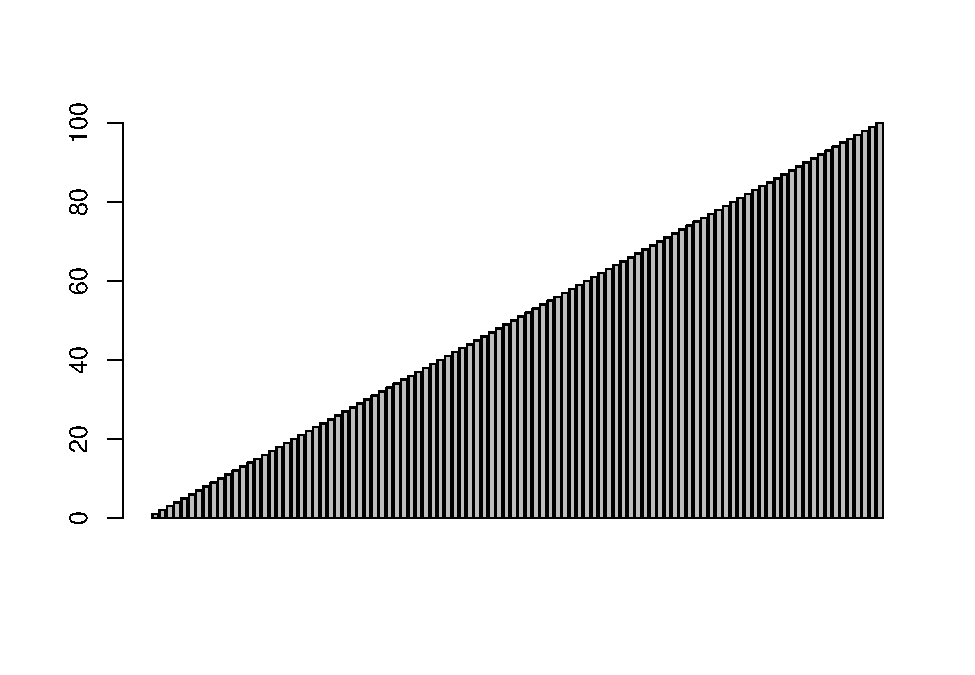
\includegraphics{TudodoR_files/figure-latex/unnamed-chunk-35-1.pdf}

\hypertarget{operauxe7uxf5es-matemuxe1ticas}{%
\subsection{Operações matemáticas}\label{operauxe7uxf5es-matemuxe1ticas}}

A maioria das operações aritméticas funcionam tão bem em vetores quanto em valores únicos. Vamos fazer outro vetor de exemplo para você trabalhar e armazená-lo na variável \textbf{a}.

Se você adicionar um escalar (um único valor) a um vetor, o escalar será adicionado a cada valor no vetor, retornando um novo vetor com os resultados. Tente adicionar 1 a cada elemento em nosso vetor:

\begin{Shaded}
\begin{Highlighting}[]
\NormalTok{a <-}\StringTok{ }\KeywordTok{c}\NormalTok{(}\DecValTok{1}\NormalTok{, }\DecValTok{2}\NormalTok{, }\DecValTok{3}\NormalTok{)}
\NormalTok{a }\OperatorTok{+}\StringTok{ }\DecValTok{1}
\end{Highlighting}
\end{Shaded}

\begin{verbatim}
## [1] 2 3 4
\end{verbatim}

O mesmo se aplica na divisão, multiplicação ou qualquer outra aritmética básica. Tente dividir nosso vetor por 2:

\begin{Shaded}
\begin{Highlighting}[]
\NormalTok{a }\OperatorTok{/}\StringTok{ }\DecValTok{2}
\end{Highlighting}
\end{Shaded}

\begin{verbatim}
## [1] 0.5 1.0 1.5
\end{verbatim}

Tente multiplicar nosso vetor por 2:

\begin{Shaded}
\begin{Highlighting}[]
\NormalTok{a}\OperatorTok{*}\DecValTok{2}
\end{Highlighting}
\end{Shaded}

\begin{verbatim}
## [1] 2 4 6
\end{verbatim}

Se você adicionar dois vetores, o R irá tirar cada valor de cada vetor e adicioná-los. Vamos fazer um segundo vetor para você experimentar e armazená-lo na variável \textbf{b}.

Tente adicioná-lo no vetor \textbf{a}:

\begin{Shaded}
\begin{Highlighting}[]
\NormalTok{b <-}\StringTok{ }\KeywordTok{c}\NormalTok{(}\DecValTok{4}\NormalTok{,}\DecValTok{5}\NormalTok{,}\DecValTok{6}\NormalTok{)}
\NormalTok{a}\OperatorTok{+}\NormalTok{b}
\end{Highlighting}
\end{Shaded}

\begin{verbatim}
## [1] 5 7 9
\end{verbatim}

Agora tente subtrair b de a:

\begin{Shaded}
\begin{Highlighting}[]
\NormalTok{a}\OperatorTok{-}\NormalTok{b}
\end{Highlighting}
\end{Shaded}

\begin{verbatim}
## [1] -3 -3 -3
\end{verbatim}

Você também pode tirar dois vetores e comparar cada item. Veja quais valores nos vetores são iguais aos de um segundo vetor:

\begin{Shaded}
\begin{Highlighting}[]
\NormalTok{a }\OperatorTok{==}\StringTok{ }\KeywordTok{c}\NormalTok{(}\DecValTok{1}\NormalTok{, }\DecValTok{99}\NormalTok{, }\DecValTok{3}\NormalTok{)}
\end{Highlighting}
\end{Shaded}

\begin{verbatim}
## [1]  TRUE FALSE  TRUE
\end{verbatim}

Observe que o R não testou se os vetores inteiros eram iguais, mas verificou cada valor no vetor a contar o valor no mesmo índice no nosso novo vetor.

Verifique se cada valor nos vetores são menores que o valor correspondente em outro vetor:

\begin{Shaded}
\begin{Highlighting}[]
\NormalTok{a }\OperatorTok{<}\StringTok{ }\KeywordTok{c}\NormalTok{(}\DecValTok{1}\NormalTok{, }\DecValTok{99}\NormalTok{, }\DecValTok{3}\NormalTok{)}
\end{Highlighting}
\end{Shaded}

\begin{verbatim}
## [1] FALSE  TRUE FALSE
\end{verbatim}

Funções que normalmente funcionam com escalares também podem operar em cada elemento de um vetor. Tente obter o seno de cada valor em nosso vetor:

\begin{Shaded}
\begin{Highlighting}[]
\KeywordTok{sin}\NormalTok{(a)}
\end{Highlighting}
\end{Shaded}

\begin{verbatim}
## [1] 0.8414710 0.9092974 0.1411200
\end{verbatim}

Agora tente obter as raízes quadradas com a função \texttt{sqrt}:

\begin{Shaded}
\begin{Highlighting}[]
\KeywordTok{sqrt}\NormalTok{(a)}
\end{Highlighting}
\end{Shaded}

\begin{verbatim}
## [1] 1.000000 1.414214 1.732051
\end{verbatim}

\hypertarget{parcelas-de-dispersuxe3o}{%
\subsection{Parcelas de dispersão}\label{parcelas-de-dispersuxe3o}}

A função \texttt{plot} leva dois vetores, um para valores X e um para valores Y, e desenha um gráfico com eles.

Vamos desenhar um gráfico que mostre a relação de números e seus senos.

Primeiro, precisaremos de alguns dados de amostra. Criaremos um vetor com alguns valores fracionários entre 0 e 20, e iremos armazenó-lo na variável x. E na variável y um segundo vetor com os senos de x:

\begin{Shaded}
\begin{Highlighting}[]
\NormalTok{x <-}\StringTok{ }\KeywordTok{seq}\NormalTok{(}\DecValTok{1}\NormalTok{, }\DecValTok{20}\NormalTok{, }\FloatTok{0.1}\NormalTok{)}
\NormalTok{y<-}\KeywordTok{sin}\NormalTok{(x)}
\end{Highlighting}
\end{Shaded}

Em seguida basta chamar a função \texttt{plot} com seus dois vetores:

\begin{Shaded}
\begin{Highlighting}[]
\KeywordTok{plot}\NormalTok{(x, y)}
\end{Highlighting}
\end{Shaded}

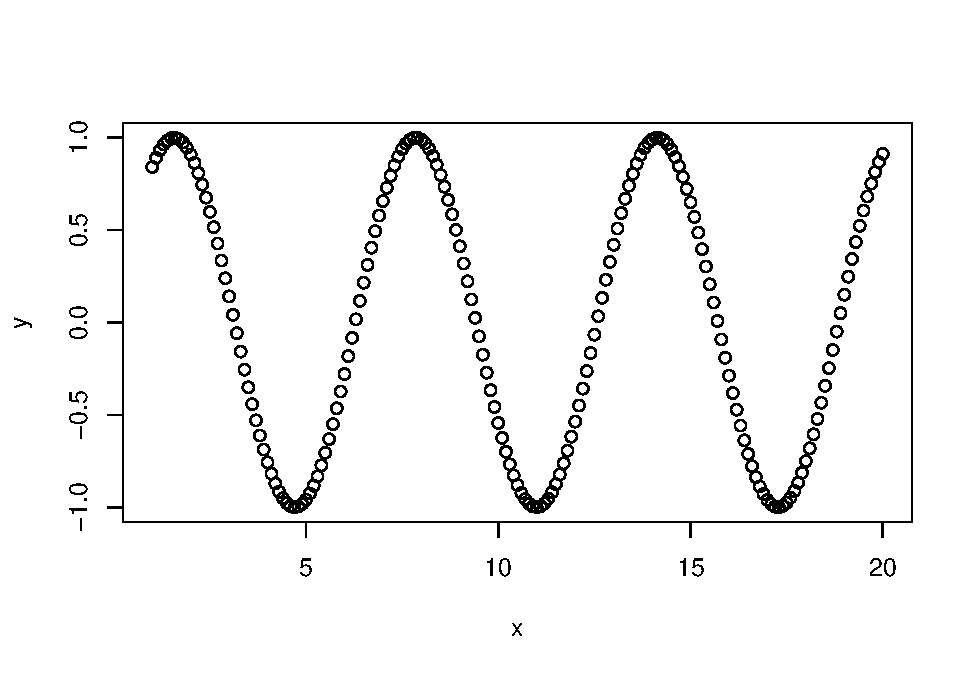
\includegraphics{TudodoR_files/figure-latex/unnamed-chunk-46-1.pdf}

Observa-se sobre o gráfico que os valores do primeiro argumento \textbf{(x)} são usados para o eixo horizontal, e os valores do segundo \textbf{(y)} para o vertical.

Vamos criar um vetor com alguns valores negativos e positivos e armazenó-lo na variável \textbf{valores}.

Também criaremos um segundo vetor com os valores absolutos do primeiro e armazenó-lo na variável \textbf{absoluto}.

Tente traçar os vetores, com os \textbf{valores} absolutos no eixo horizontal e no eixo vertical:

\begin{Shaded}
\begin{Highlighting}[]
\NormalTok{valores <-}\StringTok{ }\DecValTok{-10}\OperatorTok{:}\DecValTok{10}
\NormalTok{absoluto<-}\StringTok{ }\KeywordTok{abs}\NormalTok{(valores)}
\KeywordTok{plot}\NormalTok{(valores, absoluto)}
\end{Highlighting}
\end{Shaded}

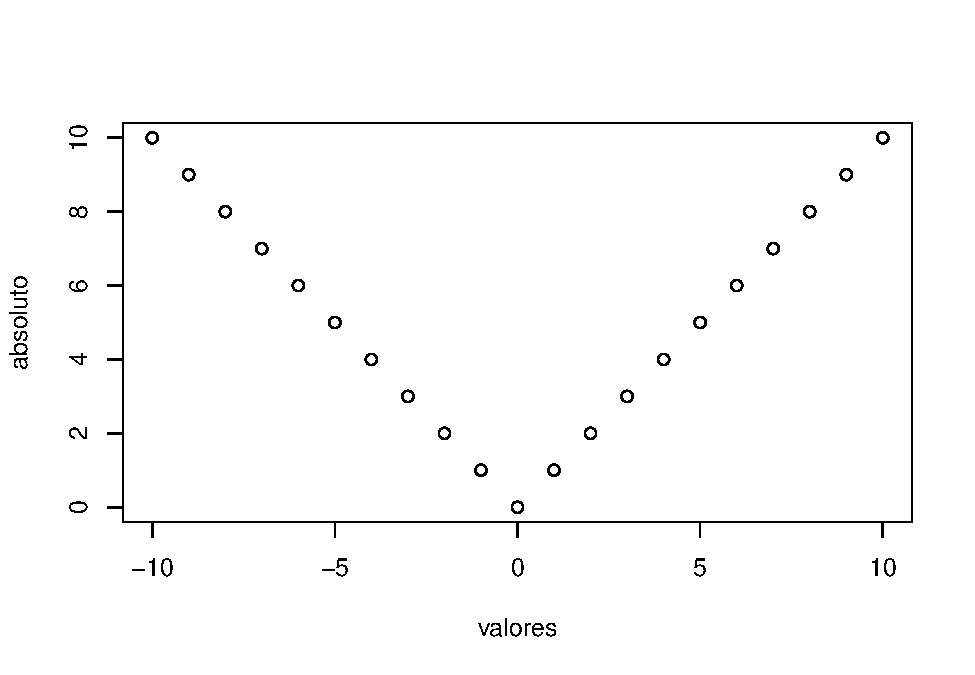
\includegraphics{TudodoR_files/figure-latex/unnamed-chunk-47-1.pdf}

\hypertarget{valores-faltantes}{%
\subsection{Valores Faltantes}\label{valores-faltantes}}

Às vezes um determinado valor não está disponível ao trabalhar com dados de amostra. Mas não é uma boa idéia apenas tirar esses valores. O R tem um valor que indica explicitamente uma amostra que não estava disponível: \textbf{NA}. Muitas funções que funcionam com vetores tratam esses valor especialmente.

Vamos criar um vetor com uma amostra ausente e armazená-lo na variével \textbf{a}.

Tente obter a soma de seus valores e veja qual é o resultado:

\begin{Shaded}
\begin{Highlighting}[]
\NormalTok{a <-}\StringTok{ }\KeywordTok{c}\NormalTok{(}\DecValTok{1}\NormalTok{, }\DecValTok{3}\NormalTok{, }\OtherTok{NA}\NormalTok{, }\DecValTok{7}\NormalTok{, }\DecValTok{9}\NormalTok{)}
\KeywordTok{sum}\NormalTok{(a)}
\end{Highlighting}
\end{Shaded}

\begin{verbatim}
## [1] NA
\end{verbatim}

A soma é considerada \emph{``não disponível''} por padrão porque um dos valores do vetor foi \textbf{NA}.

Lembre-se desse comando para mostrar ajuda para uma função. Apresente a ajuda para a função \texttt{sum}:

\begin{Shaded}
\begin{Highlighting}[]
\KeywordTok{help}\NormalTok{(sum)}
\end{Highlighting}
\end{Shaded}

Como você vê na documentação, \texttt{sum} pode tomar um argumento opcional \textbf{na.rm},. É configurado \textbf{FALSE} por padrão, mas se você configurá-lo com \textbf{TRUE}, todos os argumentos \textbf{NA} serão removidos do vetor antes do cálculo a ser executado.

Tente rondar \texttt{sum} novamente, com o \textbf{na.rm} conjunto para \textbf{TRUE}:

\begin{Shaded}
\begin{Highlighting}[]
\KeywordTok{sum}\NormalTok{(a, }\DataTypeTok{na.rm =}\NormalTok{ T)}
\end{Highlighting}
\end{Shaded}

\begin{verbatim}
## [1] 20
\end{verbatim}

\hypertarget{matrizes}{%
\section{Matrizes}\label{matrizes}}

Há varias formas de criar uma matriz. O comando \texttt{matriz()} recebe um vetor como argumento e o transfoma em uma matrix de acordo com as dimensões.
Vamos fazer uma matriz de 3 linhas de altura por 4 colunas de largura com todos os seus campos definidos em 0.

\begin{Shaded}
\begin{Highlighting}[]
\KeywordTok{matrix}\NormalTok{(}\DecValTok{0}\NormalTok{,}\DecValTok{3}\NormalTok{,}\DecValTok{4}\NormalTok{)}
\end{Highlighting}
\end{Shaded}

\begin{verbatim}
##      [,1] [,2] [,3] [,4]
## [1,]    0    0    0    0
## [2,]    0    0    0    0
## [3,]    0    0    0    0
\end{verbatim}

Você também pode usar um vetor para inicializar o valor de uma matriz. Para preencher uma matriz de 3x4, você precisará de um vetor de 12 itens.

\begin{Shaded}
\begin{Highlighting}[]
\NormalTok{a <-}\StringTok{ }\NormalTok{(}\DecValTok{1}\OperatorTok{:}\DecValTok{12}\NormalTok{)}

\KeywordTok{print}\NormalTok{ (a)}
\end{Highlighting}
\end{Shaded}

\begin{verbatim}
##  [1]  1  2  3  4  5  6  7  8  9 10 11 12
\end{verbatim}

Agora chame a matrix com o vetor, o número de linhas e o número de colunas:

\begin{Shaded}
\begin{Highlighting}[]
\KeywordTok{matrix}\NormalTok{ (a,}\CommentTok{# chama o vetor}
        \DecValTok{3}\NormalTok{,}\CommentTok{# linha}
        \DecValTok{4}\NormalTok{) }\CommentTok{#coluna}
\end{Highlighting}
\end{Shaded}

\begin{verbatim}
##      [,1] [,2] [,3] [,4]
## [1,]    1    4    7   10
## [2,]    2    5    8   11
## [3,]    3    6    9   12
\end{verbatim}

Você também pode usar um vetor para inicializar o valor de uma matriz. Para preencher uma matriz 3x4, você precisará de um vetor de 12 itens:

\begin{Shaded}
\begin{Highlighting}[]
\NormalTok{a <-}\DecValTok{1}\OperatorTok{:}\DecValTok{12}
\NormalTok{a}
\end{Highlighting}
\end{Shaded}

\begin{verbatim}
##  [1]  1  2  3  4  5  6  7  8  9 10 11 12
\end{verbatim}

Agora chame a \textbf{matrix} com o vetor, o número de linhas e o número de colunas:

\begin{Shaded}
\begin{Highlighting}[]
\KeywordTok{matrix}\NormalTok{ (a,}\DecValTok{3}\NormalTok{,}\DecValTok{4}\NormalTok{)}
\end{Highlighting}
\end{Shaded}

\begin{verbatim}
##      [,1] [,2] [,3] [,4]
## [1,]    1    4    7   10
## [2,]    2    5    8   11
## [3,]    3    6    9   12
\end{verbatim}

\hypertarget{outras-formas}{%
\subsection{Outras formas}\label{outras-formas}}

\begin{Shaded}
\begin{Highlighting}[]
\KeywordTok{matrix}\NormalTok{ (a, }\DecValTok{3}\NormalTok{)}
\end{Highlighting}
\end{Shaded}

\begin{verbatim}
##      [,1] [,2] [,3] [,4]
## [1,]    1    4    7   10
## [2,]    2    5    8   11
## [3,]    3    6    9   12
\end{verbatim}

Note que as matrizes são preenchidas ao longo das colunas. Para que a matriz seja preenchida por linhas deve-se alterar o argumento \textbf{byrow}, que por padrão está definido como \textbf{FALSE}, passe para \textbf{TRUE}:

\begin{Shaded}
\begin{Highlighting}[]
\KeywordTok{matrix}\NormalTok{(a,}\DecValTok{3}\NormalTok{, }\DataTypeTok{byrow=}\NormalTok{T)}
\end{Highlighting}
\end{Shaded}

\begin{verbatim}
##      [,1] [,2] [,3] [,4]
## [1,]    1    2    3    4
## [2,]    5    6    7    8
## [3,]    9   10   11   12
\end{verbatim}

Os valores do vetor são copiados um por um para a nova matriz. Você também pode reformular o próprio \textbf{vetor} em uma \textbf{matriz}. Crie um vetor de 8 itens:

\begin{Shaded}
\begin{Highlighting}[]
\NormalTok{foliar <-}\StringTok{ }\DecValTok{1}\OperatorTok{:}\DecValTok{8}
\end{Highlighting}
\end{Shaded}

A função \texttt{dim} define as dimensões para uma matriz. Ele aceita um vetor com o número de linhas e o número de colunas a serem atribuídas.
Atribua novas dimensões para \textbf{foliar} passando um vetor especificando 2 linhas e 4 colunas ( c(2, 4)):

\begin{Shaded}
\begin{Highlighting}[]
\KeywordTok{dim}\NormalTok{(foliar) <-}\StringTok{ }\KeywordTok{c}\NormalTok{(}\DecValTok{2}\NormalTok{,}\DecValTok{4}\NormalTok{)}
\end{Highlighting}
\end{Shaded}

O vetor não é mais unidimensional. Foi convertido no local para uma matriz.
Agora, use a função \textbf{matrix} para criar uma matriz \textbf{5x5}, com seus campos inicializados para qualquer valor que você desejar:

\begin{Shaded}
\begin{Highlighting}[]
\KeywordTok{matrix}\NormalTok{ (}\DecValTok{2}\NormalTok{,}\DecValTok{5}\NormalTok{,}\DecValTok{5}\NormalTok{)}
\end{Highlighting}
\end{Shaded}

\begin{verbatim}
##      [,1] [,2] [,3] [,4] [,5]
## [1,]    2    2    2    2    2
## [2,]    2    2    2    2    2
## [3,]    2    2    2    2    2
## [4,]    2    2    2    2    2
## [5,]    2    2    2    2    2
\end{verbatim}

\hypertarget{acesso-a-matriz}{%
\subsection{Acesso a Matriz}\label{acesso-a-matriz}}

Obter valores de matrizes não é diferente de vetores, você só precisa fornecer dois índices em vez de um. Abra a matriz foliar:

\begin{Shaded}
\begin{Highlighting}[]
\KeywordTok{print}\NormalTok{ (foliar)}
\end{Highlighting}
\end{Shaded}

\begin{verbatim}
##      [,1] [,2] [,3] [,4]
## [1,]    1    3    5    7
## [2,]    2    4    6    8
\end{verbatim}

Tente obter o valor da segunda linha na terceira coluna da matriz foliar:

\begin{Shaded}
\begin{Highlighting}[]
\NormalTok{foliar[}\DecValTok{2}\NormalTok{,}\DecValTok{3}\NormalTok{]}
\end{Highlighting}
\end{Shaded}

\begin{verbatim}
## [1] 6
\end{verbatim}

O valor da primeira linha da quarta coluna:

\begin{Shaded}
\begin{Highlighting}[]
\NormalTok{foliar[}\DecValTok{1}\NormalTok{,}\DecValTok{4}\NormalTok{]}
\end{Highlighting}
\end{Shaded}

\begin{verbatim}
## [1] 7
\end{verbatim}

Você pode obter uma linha inteira da matriz omitindo o índice da coluna (mas mantenha a virgula). Tente recuperar a segunda linha:

\begin{Shaded}
\begin{Highlighting}[]
\NormalTok{foliar[}\DecValTok{2}\NormalTok{,]}
\end{Highlighting}
\end{Shaded}

\begin{verbatim}
## [1] 2 4 6 8
\end{verbatim}

Para obter uma coluna inteira, omita o índice da linha. Recupere a quarta coluna:

\begin{Shaded}
\begin{Highlighting}[]
\NormalTok{foliar[,}\DecValTok{4}\NormalTok{]}
\end{Highlighting}
\end{Shaded}

\begin{verbatim}
## [1] 7 8
\end{verbatim}

Você pode ler várias linhas ou colunas, fornecendo um vetor ou sequência com seus índices. Tente recuperar as colunas de 2 a 4:

\begin{Shaded}
\begin{Highlighting}[]
\NormalTok{foliar[,}\DecValTok{2}\OperatorTok{:}\DecValTok{4}\NormalTok{]}
\end{Highlighting}
\end{Shaded}

\begin{verbatim}
##      [,1] [,2] [,3]
## [1,]    3    5    7
## [2,]    4    6    8
\end{verbatim}

O comando \texttt{summary} pode ser usado para obter informações da matriz

\begin{Shaded}
\begin{Highlighting}[]
\KeywordTok{summary}\NormalTok{(foliar)}
\end{Highlighting}
\end{Shaded}

\begin{verbatim}
##        V1             V2             V3             V4      
##  Min.   :1.00   Min.   :3.00   Min.   :5.00   Min.   :7.00  
##  1st Qu.:1.25   1st Qu.:3.25   1st Qu.:5.25   1st Qu.:7.25  
##  Median :1.50   Median :3.50   Median :5.50   Median :7.50  
##  Mean   :1.50   Mean   :3.50   Mean   :5.50   Mean   :7.50  
##  3rd Qu.:1.75   3rd Qu.:3.75   3rd Qu.:5.75   3rd Qu.:7.75  
##  Max.   :2.00   Max.   :4.00   Max.   :6.00   Max.   :8.00
\end{verbatim}

Se desejar um resumo de todos os elementos da matriz, basta transformá-la em um vetor:

\begin{Shaded}
\begin{Highlighting}[]
\KeywordTok{summary}\NormalTok{(}\KeywordTok{as.vector}\NormalTok{(foliar))}
\end{Highlighting}
\end{Shaded}

\begin{verbatim}
##    Min. 1st Qu.  Median    Mean 3rd Qu.    Max. 
##    1.00    2.75    4.50    4.50    6.25    8.00
\end{verbatim}

\hypertarget{visualizauxe7uxf5es-em-dados-matriciais}{%
\subsection{Visualizações em dados matriciais}\label{visualizauxe7uxf5es-em-dados-matriciais}}

Com um mapa de elevação. Tudo fica a 1 metro acima do nível do mar. Vamos criar uma matriz de 10 por 10 com todos os seus valores inicializados para 1:

\begin{Shaded}
\begin{Highlighting}[]
\NormalTok{elevacao <-}\StringTok{ }\KeywordTok{matrix}\NormalTok{ (}\DecValTok{1}\NormalTok{,}\DecValTok{10}\NormalTok{,}\DecValTok{10}\NormalTok{)}
\end{Highlighting}
\end{Shaded}

Na quarta linha, sexta coluna, defina a elevação para 0:

\begin{Shaded}
\begin{Highlighting}[]
\NormalTok{elevacao [}\DecValTok{4}\NormalTok{, }\DecValTok{6}\NormalTok{] <-}\StringTok{ }\DecValTok{0}
\end{Highlighting}
\end{Shaded}

Mapa de contorno dos valores passando a matriz para a função \texttt{contour}:

\begin{Shaded}
\begin{Highlighting}[]
\KeywordTok{contour}\NormalTok{(elevacao)}
\end{Highlighting}
\end{Shaded}

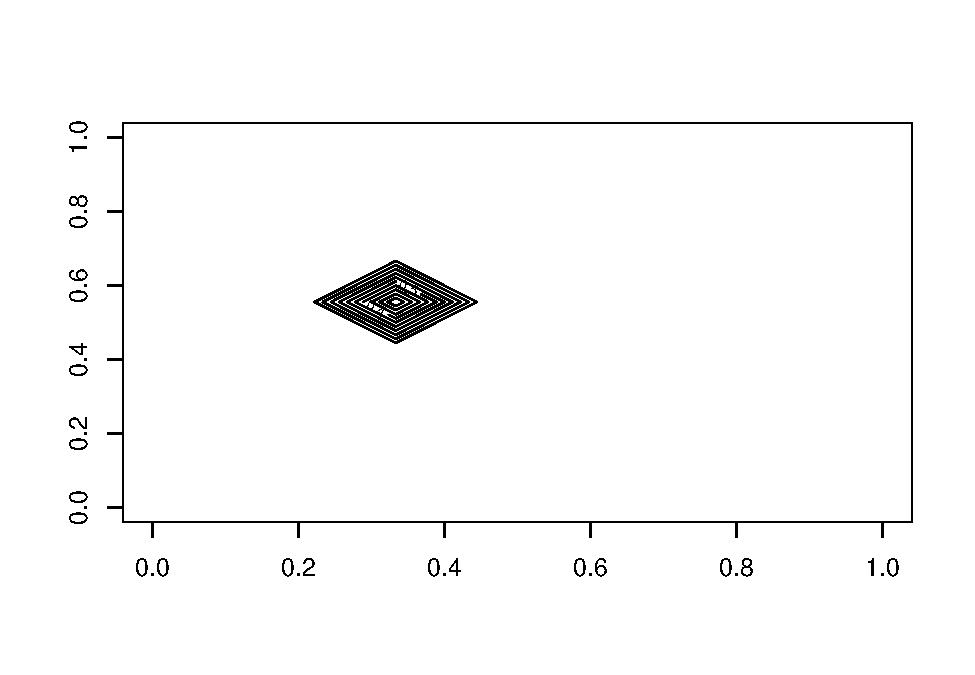
\includegraphics{TudodoR_files/figure-latex/unnamed-chunk-71-1.pdf}

Criar um gráfico em perspectiva 3D com a função \texttt{persp}:

\begin{Shaded}
\begin{Highlighting}[]
\KeywordTok{persp}\NormalTok{ (elevacao)}
\end{Highlighting}
\end{Shaded}

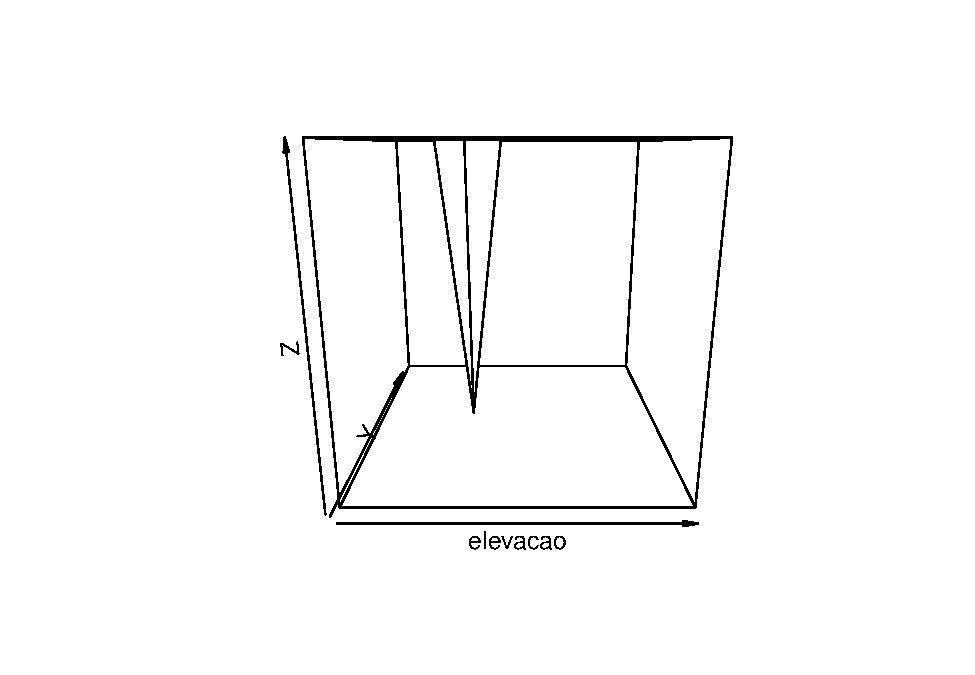
\includegraphics{TudodoR_files/figure-latex/unnamed-chunk-72-1.pdf}

Podemos consertar isso especificando nosso próprio valor para o parâmetro \textbf{expand}:

\begin{Shaded}
\begin{Highlighting}[]
\KeywordTok{persp}\NormalTok{ (elevacao, }\DataTypeTok{expand =}\FloatTok{0.2}\NormalTok{)}
\end{Highlighting}
\end{Shaded}

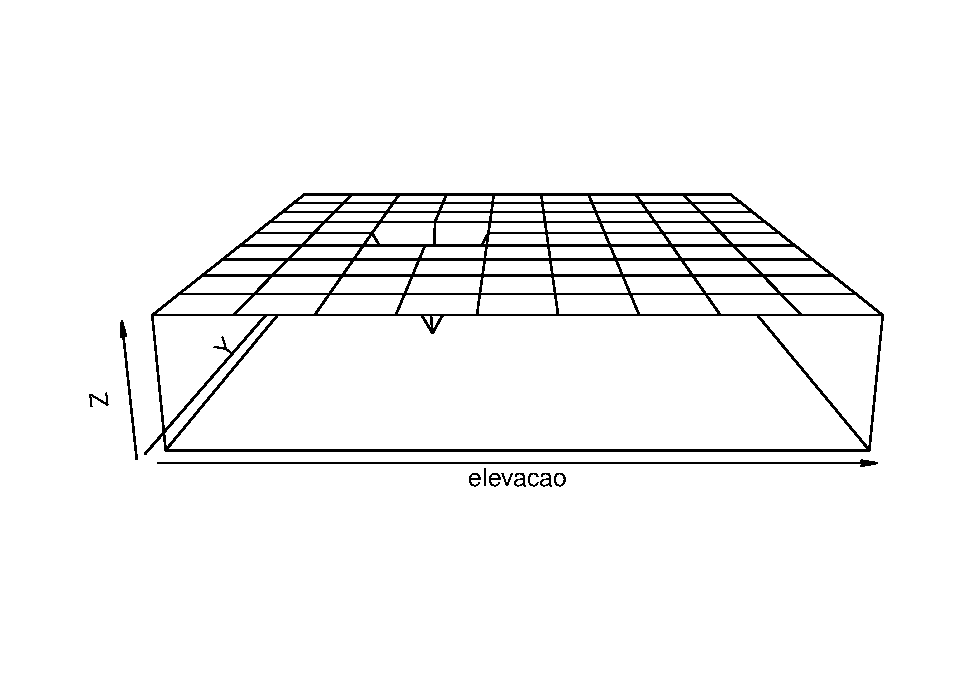
\includegraphics{TudodoR_files/figure-latex/unnamed-chunk-73-1.pdf}

O R inclui alguns conjuntos de dados de amostra. Um deles é o \emph{volcanoum} mapa 3D de um vulcão adormecido da Nova Zelândia.

É simplesmente uma matriz de 87x61 com valores de elevão, mas mostra o poder das visualizações de matriz do R. Criar um mapa de calor:

\begin{Shaded}
\begin{Highlighting}[]
\KeywordTok{contour}\NormalTok{(volcano)}
\end{Highlighting}
\end{Shaded}

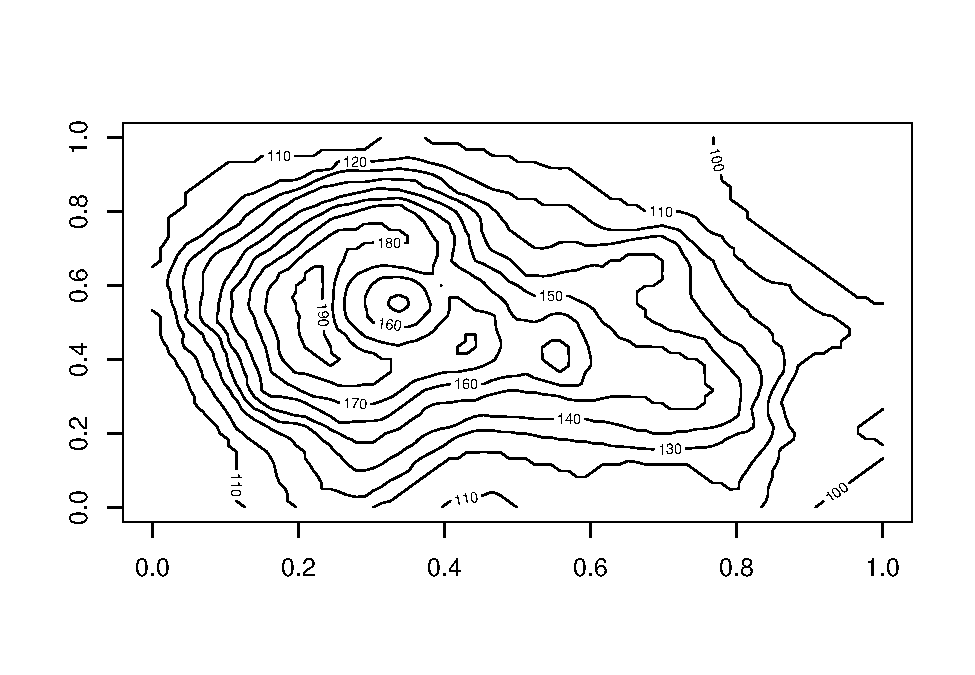
\includegraphics{TudodoR_files/figure-latex/unnamed-chunk-74-1.pdf}

Gráfico em perspectiva:

\begin{Shaded}
\begin{Highlighting}[]
\KeywordTok{persp}\NormalTok{(volcano, }\DataTypeTok{expand=}\FloatTok{0.2}\NormalTok{)}
\end{Highlighting}
\end{Shaded}

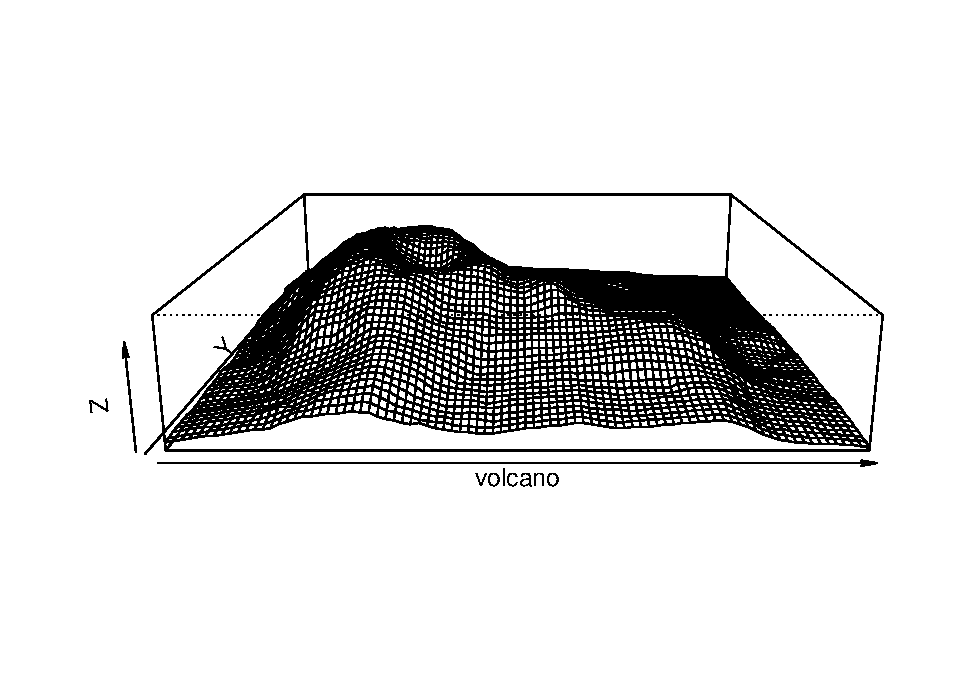
\includegraphics{TudodoR_files/figure-latex/unnamed-chunk-75-1.pdf}

A função \texttt{image} cria um mapa de calor:

\begin{Shaded}
\begin{Highlighting}[]
\KeywordTok{image}\NormalTok{(volcano)}
\end{Highlighting}
\end{Shaded}

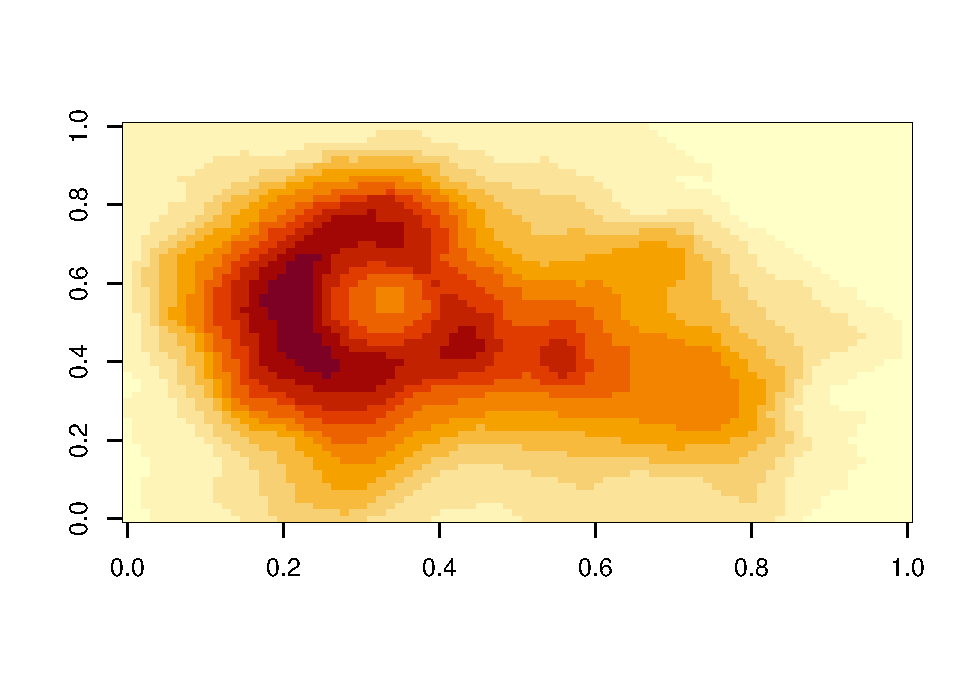
\includegraphics{TudodoR_files/figure-latex/unnamed-chunk-76-1.pdf}

\hypertarget{mais-informauxe7uxf5es-sobre-construuxe7uxf5es-de-matrizes}{%
\subsection{Mais informações sobre construções de Matrizes}\label{mais-informauxe7uxf5es-sobre-construuxe7uxf5es-de-matrizes}}

Há outros comandos que podem ser usados para construir matrizes como \texttt{cbind()} e \texttt{rbind\ ()}. Esses comandos concatenam colunas ou linhas, respectivamente na matriz (ou vetor):

\begin{Shaded}
\begin{Highlighting}[]
\NormalTok{a <-}\StringTok{ }\KeywordTok{matrix}\NormalTok{ (}\DecValTok{10}\OperatorTok{:}\DecValTok{1}\NormalTok{,}\DataTypeTok{ncol=}\DecValTok{2}\NormalTok{) }\CommentTok{#construir uma matriz qualquer}
\NormalTok{a}
\end{Highlighting}
\end{Shaded}

\begin{verbatim}
##      [,1] [,2]
## [1,]   10    5
## [2,]    9    4
## [3,]    8    3
## [4,]    7    2
## [5,]    6    1
\end{verbatim}

\begin{Shaded}
\begin{Highlighting}[]
\NormalTok{b <-}\StringTok{ }\KeywordTok{cbind}\NormalTok{ (a,}\DecValTok{1}\OperatorTok{:}\DecValTok{5}\NormalTok{) }\CommentTok{#adicionar uma terceira coluna}
\NormalTok{b}
\end{Highlighting}
\end{Shaded}

\begin{verbatim}
##      [,1] [,2] [,3]
## [1,]   10    5    1
## [2,]    9    4    2
## [3,]    8    3    3
## [4,]    7    2    4
## [5,]    6    1    5
\end{verbatim}

\begin{Shaded}
\begin{Highlighting}[]
\NormalTok{c<-}\StringTok{ }\KeywordTok{rbind}\NormalTok{(b,}\KeywordTok{c}\NormalTok{(}\DecValTok{28}\NormalTok{,}\DecValTok{28}\NormalTok{,}\DecValTok{28}\NormalTok{))}
\NormalTok{c}
\end{Highlighting}
\end{Shaded}

\begin{verbatim}
##      [,1] [,2] [,3]
## [1,]   10    5    1
## [2,]    9    4    2
## [3,]    8    3    3
## [4,]    7    2    4
## [5,]    6    1    5
## [6,]   28   28   28
\end{verbatim}

Opcionalmente matrizes podem ter nomes associados às linhas e colunas (``rownames''e ``colnames''). Cada um destes componentes da matrix é um vetor de nomes.

\begin{Shaded}
\begin{Highlighting}[]
\NormalTok{m1 <-}\StringTok{ }\KeywordTok{matrix}\NormalTok{(}\DecValTok{1}\OperatorTok{:}\DecValTok{12}\NormalTok{, }\DataTypeTok{ncol =} \DecValTok{3}\NormalTok{) }

\KeywordTok{dimnames}\NormalTok{(m1) <-}\StringTok{ }\KeywordTok{list}\NormalTok{(}\KeywordTok{c}\NormalTok{(}\StringTok{"L1"}\NormalTok{, }\StringTok{"L2"}\NormalTok{, }\StringTok{"L3"}\NormalTok{, }\StringTok{"L4"}\NormalTok{), }\KeywordTok{c}\NormalTok{(}\StringTok{"C1"}\NormalTok{, }\StringTok{"C2"}\NormalTok{, }\StringTok{"C3"}\NormalTok{)) }
\KeywordTok{dimnames}\NormalTok{(m1)}
\end{Highlighting}
\end{Shaded}

\begin{verbatim}
## [[1]]
## [1] "L1" "L2" "L3" "L4"
## 
## [[2]]
## [1] "C1" "C2" "C3"
\end{verbatim}

Matrizes são muitas vezes utilizadas para armazenar frequências de cruzamentos entre variáveis. Desta forma é comum surgir a necessidade de obter os totais marginais, isto é a soma dos elementos das linhas e/ou colunas das matrizes, o que pode ser diretamente obtido com \texttt{margin.table(\ )}:

\begin{Shaded}
\begin{Highlighting}[]
 \KeywordTok{margin.table}\NormalTok{(m1, }\DataTypeTok{margin =} \DecValTok{1}\NormalTok{)}
\end{Highlighting}
\end{Shaded}

\begin{verbatim}
## L1 L2 L3 L4 
## 15 18 21 24
\end{verbatim}

\begin{Shaded}
\begin{Highlighting}[]
 \KeywordTok{margin.table}\NormalTok{(m1, }\DataTypeTok{margin =} \DecValTok{2}\NormalTok{)}
\end{Highlighting}
\end{Shaded}

\begin{verbatim}
## C1 C2 C3 
## 10 26 42
\end{verbatim}

\begin{Shaded}
\begin{Highlighting}[]
 \KeywordTok{apply}\NormalTok{(m1, }\DecValTok{2}\NormalTok{, median)}
\end{Highlighting}
\end{Shaded}

\begin{verbatim}
##   C1   C2   C3 
##  2.5  6.5 10.5
\end{verbatim}

\hypertarget{fatores}{%
\section{Fatores}\label{fatores}}

Os fatores são vetores em que os elementos pertencem a uma ou mais categorias temáticas. Por exemplo, ao criar um vetor de indicadores de \textbf{``tratamentos''} em uma análise de experimentos, devemos declarar este vetor como um \textbf{``fator''}.
Pode criar um fator usando o comando \textbf{factor()}, ou o comando \textbf{gl}.

\begin{Shaded}
\begin{Highlighting}[]
\KeywordTok{factor}\NormalTok{(}\KeywordTok{rep}\NormalTok{(}\KeywordTok{paste}\NormalTok{(}\StringTok{"T"}\NormalTok{, }\DecValTok{1}\OperatorTok{:}\DecValTok{3}\NormalTok{, }\DataTypeTok{sep =} \StringTok{""}\NormalTok{), }\KeywordTok{c}\NormalTok{(}\DecValTok{4}\NormalTok{, }\DecValTok{4}\NormalTok{, }\DecValTok{3}\NormalTok{)))}
\end{Highlighting}
\end{Shaded}

\begin{verbatim}
##  [1] T1 T1 T1 T1 T2 T2 T2 T2 T3 T3 T3
## Levels: T1 T2 T3
\end{verbatim}

\begin{Shaded}
\begin{Highlighting}[]
\NormalTok{peso  <-}\StringTok{ }\KeywordTok{c}\NormalTok{(}\FloatTok{134.8}\NormalTok{, }\FloatTok{139.7}\NormalTok{, }\FloatTok{147.6}\NormalTok{, }\FloatTok{132.3}\NormalTok{, }\FloatTok{161.7}\NormalTok{, }\FloatTok{157.7}\NormalTok{, }\FloatTok{150.3}\NormalTok{, }\FloatTok{144.7}\NormalTok{,}
           \FloatTok{160.7}\NormalTok{, }\FloatTok{172.7}\NormalTok{, }\FloatTok{163.4}\NormalTok{, }\FloatTok{161.3}\NormalTok{, }\FloatTok{169.8}\NormalTok{, }\FloatTok{168.2}\NormalTok{, }\FloatTok{160.7}\NormalTok{, }\FloatTok{161.0}\NormalTok{,}
           \FloatTok{165.7}\NormalTok{, }\FloatTok{160.0}\NormalTok{, }\FloatTok{158.2}\NormalTok{, }\FloatTok{151.0}\NormalTok{, }\FloatTok{171.8}\NormalTok{, }\FloatTok{157.3}\NormalTok{, }\FloatTok{150.4}\NormalTok{, }\FloatTok{160.4}\NormalTok{,}
           \FloatTok{154.5}\NormalTok{, }\FloatTok{160.4}\NormalTok{, }\FloatTok{148.8}\NormalTok{, }\FloatTok{154.0}\NormalTok{)}
\NormalTok{trat  <-}\StringTok{ }\KeywordTok{rep}\NormalTok{(}\KeywordTok{seq}\NormalTok{(}\DecValTok{0}\NormalTok{,}\DecValTok{300}\NormalTok{,}\DecValTok{50}\NormalTok{), }\DataTypeTok{each=}\DecValTok{4}\NormalTok{)  }\CommentTok{#?each}
\NormalTok{dados <-}\StringTok{  }\KeywordTok{data.frame}\NormalTok{(peso, }\DataTypeTok{trat=}\KeywordTok{as.factor}\NormalTok{(trat))}
\end{Highlighting}
\end{Shaded}

\hypertarget{array}{%
\section{Array}\label{array}}

O conceito de array generaliza a idéia de matrix. Enquanto em uma matrix os elementos são organizados em duas dimensões (linhas e colunas), em um array os elementos podem ser organizados em um número arbitrário de dimensões.
No R um array é definido utilizando a função \texttt{array()}:

\begin{Shaded}
\begin{Highlighting}[]
\NormalTok{ar1 <-}\StringTok{ }\KeywordTok{array}\NormalTok{(}\DecValTok{1}\OperatorTok{:}\DecValTok{24}\NormalTok{, }\DataTypeTok{dim =} \KeywordTok{c}\NormalTok{(}\DecValTok{3}\NormalTok{, }\DecValTok{4}\NormalTok{, }\DecValTok{2}\NormalTok{)) }
\NormalTok{ar1}
\end{Highlighting}
\end{Shaded}

\begin{verbatim}
## , , 1
## 
##      [,1] [,2] [,3] [,4]
## [1,]    1    4    7   10
## [2,]    2    5    8   11
## [3,]    3    6    9   12
## 
## , , 2
## 
##      [,1] [,2] [,3] [,4]
## [1,]   13   16   19   22
## [2,]   14   17   20   23
## [3,]   15   18   21   24
\end{verbatim}

Veja agora um exemplo de dados já incluído no R no formato de array. Para ``carregar'' e visualizar os dados digite:

\begin{Shaded}
\begin{Highlighting}[]
\KeywordTok{data}\NormalTok{(Titanic) }
\NormalTok{Titanic}
\end{Highlighting}
\end{Shaded}

\begin{verbatim}
## , , Age = Child, Survived = No
## 
##       Sex
## Class  Male Female
##   1st     0      0
##   2nd     0      0
##   3rd    35     17
##   Crew    0      0
## 
## , , Age = Adult, Survived = No
## 
##       Sex
## Class  Male Female
##   1st   118      4
##   2nd   154     13
##   3rd   387     89
##   Crew  670      3
## 
## , , Age = Child, Survived = Yes
## 
##       Sex
## Class  Male Female
##   1st     5      1
##   2nd    11     13
##   3rd    13     14
##   Crew    0      0
## 
## , , Age = Adult, Survived = Yes
## 
##       Sex
## Class  Male Female
##   1st    57    140
##   2nd    14     80
##   3rd    75     76
##   Crew  192     20
\end{verbatim}

Para obter maiores informações sobre estes dados digite: \texttt{help(Titanic)}

Agora vamos responder às seguintes perguntas, mostrando os comandos do R utilizados sobre o array de dados.

\begin{enumerate}
\def\labelenumi{\arabic{enumi}.}
\tightlist
\item
  Quantas pessoas haviam no total?
\end{enumerate}

\begin{Shaded}
\begin{Highlighting}[]
\KeywordTok{sum}\NormalTok{(Titanic)}
\end{Highlighting}
\end{Shaded}

\begin{verbatim}
## [1] 2201
\end{verbatim}

\begin{enumerate}
\def\labelenumi{\arabic{enumi}.}
\setcounter{enumi}{1}
\tightlist
\item
  Quantas pessoas haviam na tripulação (crew)?
\end{enumerate}

\begin{Shaded}
\begin{Highlighting}[]
\KeywordTok{sum}\NormalTok{(Titanic[}\DecValTok{4}\NormalTok{, , , ])}
\end{Highlighting}
\end{Shaded}

\begin{verbatim}
## [1] 885
\end{verbatim}

\begin{enumerate}
\def\labelenumi{\arabic{enumi}.}
\setcounter{enumi}{2}
\tightlist
\item
  Quantas pessoas sobreviveram e quantas morreram?
\end{enumerate}

\begin{Shaded}
\begin{Highlighting}[]
\KeywordTok{apply}\NormalTok{(Titanic, }\DecValTok{4}\NormalTok{, sum)}
\end{Highlighting}
\end{Shaded}

\begin{verbatim}
##   No  Yes 
## 1490  711
\end{verbatim}

\begin{enumerate}
\def\labelenumi{\arabic{enumi}.}
\setcounter{enumi}{3}
\tightlist
\item
  Quais as proporções de sobreviventes entre homens e mulheres?
\end{enumerate}

\begin{Shaded}
\begin{Highlighting}[]
\KeywordTok{margin.table}\NormalTok{(Titanic, }\DataTypeTok{margin =} \DecValTok{1}\NormalTok{)}
\end{Highlighting}
\end{Shaded}

\begin{verbatim}
## Class
##  1st  2nd  3rd Crew 
##  325  285  706  885
\end{verbatim}

\begin{Shaded}
\begin{Highlighting}[]
\KeywordTok{margin.table}\NormalTok{(Titanic, }\DataTypeTok{margin =} \DecValTok{2}\NormalTok{)}
\end{Highlighting}
\end{Shaded}

\begin{verbatim}
## Sex
##   Male Female 
##   1731    470
\end{verbatim}

\begin{Shaded}
\begin{Highlighting}[]
\KeywordTok{margin.table}\NormalTok{(Titanic, }\DataTypeTok{margin =} \DecValTok{3}\NormalTok{)}
\end{Highlighting}
\end{Shaded}

\begin{verbatim}
## Age
## Child Adult 
##   109  2092
\end{verbatim}

\begin{Shaded}
\begin{Highlighting}[]
\KeywordTok{margin.table}\NormalTok{(Titanic, }\DataTypeTok{margin =} \DecValTok{4}\NormalTok{)}
\end{Highlighting}
\end{Shaded}

\begin{verbatim}
## Survived
##   No  Yes 
## 1490  711
\end{verbatim}

Esta função admite ainda índices múltiplos que permitem outros resumos da tabela de dados. Foi demonstrado como obter o total de sobreviventes e não sobreviventes, separados por sexo e depois as porcentagens de sobreviventes para cada sexo. Exemplo:

\begin{Shaded}
\begin{Highlighting}[]
\KeywordTok{margin.table}\NormalTok{(Titanic, }\DataTypeTok{margin =} \KeywordTok{c}\NormalTok{(}\DecValTok{2}\NormalTok{, }\DecValTok{4}\NormalTok{))}
\end{Highlighting}
\end{Shaded}

\begin{verbatim}
##         Survived
## Sex        No  Yes
##   Male   1364  367
##   Female  126  344
\end{verbatim}

\begin{Shaded}
\begin{Highlighting}[]
\KeywordTok{prop.table}\NormalTok{(}\KeywordTok{margin.table}\NormalTok{(Titanic, }\DataTypeTok{margin =} \KeywordTok{c}\NormalTok{(}\DecValTok{2}\NormalTok{, }\DecValTok{4}\NormalTok{)), }\DataTypeTok{margin =} \DecValTok{1}\NormalTok{)}
\end{Highlighting}
\end{Shaded}

\begin{verbatim}
##         Survived
## Sex             No       Yes
##   Male   0.7879838 0.2120162
##   Female 0.2680851 0.7319149
\end{verbatim}

\begin{Shaded}
\begin{Highlighting}[]
\KeywordTok{prop.table}\NormalTok{(}\KeywordTok{margin.table}\NormalTok{(Titanic, }\DataTypeTok{margin =} \KeywordTok{c}\NormalTok{(}\DecValTok{2}\NormalTok{, }\DecValTok{1}\NormalTok{)), }\DataTypeTok{margin =} \DecValTok{1}\NormalTok{)}
\end{Highlighting}
\end{Shaded}

\begin{verbatim}
##         Class
## Sex             1st        2nd        3rd       Crew
##   Male   0.10398614 0.10340843 0.29462738 0.49797805
##   Female 0.30851064 0.22553191 0.41702128 0.04893617
\end{verbatim}

\hypertarget{data.frame}{%
\section{Data.frame}\label{data.frame}}

Os datas.frames são muito semelhantes quando comparados às matrizes, pois têm linhas e colunas, portanto duas dimensões. Entretando, diferentemente das matrizes, colunas diferentes podem armazenar elementos de tipos diferentes. Por exemplo, a primeira coluna pode ser numérica, enquanto a segunda constituida de caracteres. Cada coluna precisa ter o mesmo tamanho.
Criar o vetor nomes:

\begin{Shaded}
\begin{Highlighting}[]
\NormalTok{nome <-}\StringTok{ }\KeywordTok{c}\NormalTok{(}\StringTok{"Melissa José"}\NormalTok{,}
          \StringTok{"Jennifer Linhares"}\NormalTok{,}
          \StringTok{"Gedilene Ponciano"}\NormalTok{,}
          \StringTok{"Edinar da Silva"}\NormalTok{,}
          \StringTok{"Osmar Emidio"}\NormalTok{,}
          \StringTok{"Jeeziel Vieira"}\NormalTok{)}
\end{Highlighting}
\end{Shaded}

Criar vetor idade:

\begin{Shaded}
\begin{Highlighting}[]
\NormalTok{idade <-}\StringTok{ }\KeywordTok{c}\NormalTok{(}\DecValTok{17}\NormalTok{,}\DecValTok{18}\NormalTok{,}\DecValTok{16}\NormalTok{,}\DecValTok{15}\NormalTok{,}\DecValTok{15}\NormalTok{,}\DecValTok{18}\NormalTok{)}
\end{Highlighting}
\end{Shaded}

Criar vetor sexo (categoria=fator):

\begin{Shaded}
\begin{Highlighting}[]
\NormalTok{sexo <-}\StringTok{ }\KeywordTok{factor}\NormalTok{(}\KeywordTok{c}\NormalTok{(}\StringTok{"F"}\NormalTok{,}\StringTok{"F"}\NormalTok{,}\StringTok{"F"}\NormalTok{,}\StringTok{"F"}\NormalTok{,}\StringTok{"M"}\NormalTok{,}\StringTok{"M"}\NormalTok{))}
\end{Highlighting}
\end{Shaded}

Criar vetor altura:

\begin{Shaded}
\begin{Highlighting}[]
\NormalTok{alt <-}\StringTok{ }\KeywordTok{c}\NormalTok{(}\DecValTok{180}\NormalTok{,}\DecValTok{170}\NormalTok{,}\DecValTok{160}\NormalTok{,}\DecValTok{150}\NormalTok{,}\DecValTok{140}\NormalTok{,}\DecValTok{168}\NormalTok{)}
\end{Highlighting}
\end{Shaded}

Reunir tudo em um data.frame:

\begin{Shaded}
\begin{Highlighting}[]
\NormalTok{dados <-}\StringTok{ }\KeywordTok{data.frame}\NormalTok{(nome, idade, sexo, alt)}
\end{Highlighting}
\end{Shaded}

Ver atributos da tabela:

\begin{Shaded}
\begin{Highlighting}[]
\KeywordTok{str}\NormalTok{(dados)}
\end{Highlighting}
\end{Shaded}

\begin{verbatim}
## 'data.frame':    6 obs. of  4 variables:
##  $ nome : Factor w/ 6 levels "Edinar da Silva",..: 5 4 2 1 6 3
##  $ idade: num  17 18 16 15 15 18
##  $ sexo : Factor w/ 2 levels "F","M": 1 1 1 1 2 2
##  $ alt  : num  180 170 160 150 140 168
\end{verbatim}

Adicionar nome às linhas com o comando \texttt{row.names()}:

\begin{Shaded}
\begin{Highlighting}[]
\KeywordTok{row.names}\NormalTok{(dados) <-}\StringTok{ }\KeywordTok{c}\NormalTok{(}\DecValTok{1}\NormalTok{,}\DecValTok{2}\NormalTok{,}\DecValTok{3}\NormalTok{,}\DecValTok{4}\NormalTok{,}\DecValTok{5}\NormalTok{,}\DecValTok{6}\NormalTok{)}
\NormalTok{dados}
\end{Highlighting}
\end{Shaded}

\begin{verbatim}
##                nome idade sexo alt
## 1      Melissa José    17    F 180
## 2 Jennifer Linhares    18    F 170
## 3 Gedilene Ponciano    16    F 160
## 4   Edinar da Silva    15    F 150
## 5      Osmar Emidio    15    M 140
## 6    Jeeziel Vieira    18    M 168
\end{verbatim}

\begin{Shaded}
\begin{Highlighting}[]
\KeywordTok{names}\NormalTok{(dados) <-}\StringTok{ }\KeywordTok{c}\NormalTok{(}\StringTok{"Nome"}\NormalTok{, }\StringTok{"Idade"}\NormalTok{, }\StringTok{"Sexo"}\NormalTok{, }\StringTok{"altura"}\NormalTok{)}
\NormalTok{dados}
\end{Highlighting}
\end{Shaded}

\begin{verbatim}
##                Nome Idade Sexo altura
## 1      Melissa José    17    F    180
## 2 Jennifer Linhares    18    F    170
## 3 Gedilene Ponciano    16    F    160
## 4   Edinar da Silva    15    F    150
## 5      Osmar Emidio    15    M    140
## 6    Jeeziel Vieira    18    M    168
\end{verbatim}

\hypertarget{uxedndice-dos-data.frames}{%
\subsection{Índice dos Data.frames}\label{uxedndice-dos-data.frames}}

Buscar elementos:

\begin{Shaded}
\begin{Highlighting}[]
\NormalTok{dados[}\DecValTok{2}\NormalTok{,}\DecValTok{1}\NormalTok{] }\CommentTok{#elemento da  linha  2, coluna 1}
\end{Highlighting}
\end{Shaded}

\begin{verbatim}
## [1] Jennifer Linhares
## 6 Levels: Edinar da Silva Gedilene Ponciano ... Osmar Emidio
\end{verbatim}

\begin{Shaded}
\begin{Highlighting}[]
\NormalTok{dados[}\DecValTok{2}\NormalTok{,] }\CommentTok{#toda linha dois}
\end{Highlighting}
\end{Shaded}

\begin{verbatim}
##                Nome Idade Sexo altura
## 2 Jennifer Linhares    18    F    170
\end{verbatim}

Repare que apesar de ``Nomes'' ter sido criado como vetor de caracteres, o R passou a entender como um fator dentro do data.frame:

\begin{Shaded}
\begin{Highlighting}[]
\NormalTok{dados[,}\DecValTok{1}\NormalTok{]}
\end{Highlighting}
\end{Shaded}

\begin{verbatim}
## [1] Melissa José      Jennifer Linhares Gedilene Ponciano Edinar da Silva  
## [5] Osmar Emidio      Jeeziel Vieira   
## 6 Levels: Edinar da Silva Gedilene Ponciano ... Osmar Emidio
\end{verbatim}

Transformar para caracteres:

\begin{Shaded}
\begin{Highlighting}[]
\NormalTok{dados[,}\DecValTok{1}\NormalTok{] <-}\StringTok{ }\KeywordTok{as.character}\NormalTok{(dados[,}\DecValTok{1}\NormalTok{])}
\NormalTok{dados[,}\DecValTok{1}\NormalTok{]}
\end{Highlighting}
\end{Shaded}

\begin{verbatim}
## [1] "Melissa José"      "Jennifer Linhares" "Gedilene Ponciano"
## [4] "Edinar da Silva"   "Osmar Emidio"      "Jeeziel Vieira"
\end{verbatim}

Acessando os dados:

\begin{Shaded}
\begin{Highlighting}[]
\NormalTok{dados}\OperatorTok{$}\NormalTok{Nome}
\end{Highlighting}
\end{Shaded}

\begin{verbatim}
## [1] "Melissa José"      "Jennifer Linhares" "Gedilene Ponciano"
## [4] "Edinar da Silva"   "Osmar Emidio"      "Jeeziel Vieira"
\end{verbatim}

\begin{Shaded}
\begin{Highlighting}[]
\NormalTok{dados}\OperatorTok{$}\NormalTok{Nome[}\DecValTok{3}\NormalTok{]}
\end{Highlighting}
\end{Shaded}

\begin{verbatim}
## [1] "Gedilene Ponciano"
\end{verbatim}

\begin{Shaded}
\begin{Highlighting}[]
\NormalTok{dados}\OperatorTok{$}\NormalTok{Nome [}\DecValTok{1}\OperatorTok{:}\DecValTok{3}\NormalTok{]}
\end{Highlighting}
\end{Shaded}

\begin{verbatim}
## [1] "Melissa José"      "Jennifer Linhares" "Gedilene Ponciano"
\end{verbatim}

\begin{Shaded}
\begin{Highlighting}[]
\KeywordTok{str}\NormalTok{(dados)}
\end{Highlighting}
\end{Shaded}

\begin{verbatim}
## 'data.frame':    6 obs. of  4 variables:
##  $ Nome  : chr  "Melissa José" "Jennifer Linhares" "Gedilene Ponciano" "Edinar da Silva" ...
##  $ Idade : num  17 18 16 15 15 18
##  $ Sexo  : Factor w/ 2 levels "F","M": 1 1 1 1 2 2
##  $ altura: num  180 170 160 150 140 168
\end{verbatim}

\hypertarget{manipulando-um-data.frame}{%
\subsection{Manipulando um Data.frame}\label{manipulando-um-data.frame}}

Você pode manipular um data.frame adicionando ou eliminando colunas ou linhas, assim como em matrizes. Pode-se usar os comandos \texttt{cbind()} e \texttt{rbind\ ()} para adcionar colunas e linhas respectivamente a um data.frame:

\begin{Shaded}
\begin{Highlighting}[]
\NormalTok{dados <-}\StringTok{ }\KeywordTok{cbind}\NormalTok{ (dados, }\CommentTok{#adicionar uma coluna}
               \DataTypeTok{Conceito=}\KeywordTok{c}\NormalTok{(}\StringTok{"A"}\NormalTok{,}\StringTok{"A"}\NormalTok{,}\StringTok{"A"}\NormalTok{,}\StringTok{"C"}\NormalTok{,}\StringTok{"A"}\NormalTok{,}\StringTok{"B"}\NormalTok{))}
\end{Highlighting}
\end{Shaded}

\begin{Shaded}
\begin{Highlighting}[]
\NormalTok{dados <-}\StringTok{ }\KeywordTok{rbind}\NormalTok{ (dados, }\CommentTok{#adicionar uma linha}
                \StringTok{"7"}\NormalTok{=}\StringTok{ }\KeywordTok{c}\NormalTok{(}\StringTok{"Caio Pinto"}\NormalTok{, }\DecValTok{21}\NormalTok{, }\StringTok{"M"}\NormalTok{, }\DecValTok{172}\NormalTok{, }\StringTok{"C"}\NormalTok{))}
\NormalTok{dados}
\end{Highlighting}
\end{Shaded}

\begin{verbatim}
##                Nome Idade Sexo altura Conceito
## 1      Melissa José    17    F    180        A
## 2 Jennifer Linhares    18    F    170        A
## 3 Gedilene Ponciano    16    F    160        A
## 4   Edinar da Silva    15    F    150        C
## 5      Osmar Emidio    15    M    140        A
## 6    Jeeziel Vieira    18    M    168        B
## 7        Caio Pinto    21    M    172        C
\end{verbatim}

Assim como para vetores e matrizes, você pode selecionar um subgrupo de um data.frame e armazená-lo em um outro objeto ou utilizar índices como o sinal negativo para eliminar linhas ou colunas de um data.frame:

\begin{Shaded}
\begin{Highlighting}[]
\NormalTok{dados<-}\StringTok{ }\NormalTok{dados [}\DecValTok{1}\OperatorTok{:}\DecValTok{6}\NormalTok{,] }\CommentTok{#selecionar linha de 1 a 6}
\NormalTok{dados<-}\StringTok{ }\NormalTok{dados [,}\OperatorTok{-}\DecValTok{5}\NormalTok{] }\CommentTok{#excluir a quinta coluna}
\NormalTok{dados}
\end{Highlighting}
\end{Shaded}

\begin{verbatim}
##                Nome Idade Sexo altura
## 1      Melissa José    17    F    180
## 2 Jennifer Linhares    18    F    170
## 3 Gedilene Ponciano    16    F    160
## 4   Edinar da Silva    15    F    150
## 5      Osmar Emidio    15    M    140
## 6    Jeeziel Vieira    18    M    168
\end{verbatim}

\begin{Shaded}
\begin{Highlighting}[]
\NormalTok{dados[dados}\OperatorTok{$}\NormalTok{Sexo}\OperatorTok{==}\StringTok{"F"}\NormalTok{,] }\CommentTok{#exibir só masculinos}
\end{Highlighting}
\end{Shaded}

\begin{verbatim}
##                Nome Idade Sexo altura
## 1      Melissa José    17    F    180
## 2 Jennifer Linhares    18    F    170
## 3 Gedilene Ponciano    16    F    160
## 4   Edinar da Silva    15    F    150
\end{verbatim}

A ordenação das linhas de um \textbf{data.frame} segundo os dados contidos em determinadas colunas também é extremamente útil:

\begin{Shaded}
\begin{Highlighting}[]
\NormalTok{dados [}\KeywordTok{order}\NormalTok{(dados}\OperatorTok{$}\NormalTok{altura),]}
\end{Highlighting}
\end{Shaded}

\begin{verbatim}
##                Nome Idade Sexo altura
## 5      Osmar Emidio    15    M    140
## 4   Edinar da Silva    15    F    150
## 3 Gedilene Ponciano    16    F    160
## 6    Jeeziel Vieira    18    M    168
## 2 Jennifer Linhares    18    F    170
## 1      Melissa José    17    F    180
\end{verbatim}

\begin{Shaded}
\begin{Highlighting}[]
\NormalTok{dados [}\KeywordTok{rev}\NormalTok{(}\KeywordTok{order}\NormalTok{(dados}\OperatorTok{$}\NormalTok{altura)),]}
\end{Highlighting}
\end{Shaded}

\begin{verbatim}
##                Nome Idade Sexo altura
## 1      Melissa José    17    F    180
## 2 Jennifer Linhares    18    F    170
## 6    Jeeziel Vieira    18    M    168
## 3 Gedilene Ponciano    16    F    160
## 4   Edinar da Silva    15    F    150
## 5      Osmar Emidio    15    M    140
\end{verbatim}

\hypertarget{separando-um-data.frame-por-grupos}{%
\subsection{Separando um data.frame por grupos}\label{separando-um-data.frame-por-grupos}}

\begin{Shaded}
\begin{Highlighting}[]
\KeywordTok{split}\NormalTok{ (dados, sexo)}
\end{Highlighting}
\end{Shaded}

\begin{verbatim}
## $F
##                Nome Idade Sexo altura
## 1      Melissa José    17    F    180
## 2 Jennifer Linhares    18    F    170
## 3 Gedilene Ponciano    16    F    160
## 4   Edinar da Silva    15    F    150
## 
## $M
##             Nome Idade Sexo altura
## 5   Osmar Emidio    15    M    140
## 6 Jeeziel Vieira    18    M    168
\end{verbatim}

\hypertarget{lista}{%
\section{Lista}\label{lista}}

Listas são objetos muito úteis, pois são usadas para combinar diferentes estruturas de dados em um mesmo objeto, ou seja, vetores, matrizes, arrays, data.frames e até mesmo outras listas:

\begin{Shaded}
\begin{Highlighting}[]
\NormalTok{pes <-}\StringTok{ }\KeywordTok{list}\NormalTok{ (}\DataTypeTok{idade=}\DecValTok{32}\NormalTok{, }\DataTypeTok{nome=}\StringTok{"Maria"}\NormalTok{, }\DataTypeTok{notas=}\KeywordTok{c}\NormalTok{(}\DecValTok{98}\NormalTok{,}\DecValTok{95}\NormalTok{,}\DecValTok{78}\NormalTok{), }\DataTypeTok{B=}\KeywordTok{matrix}\NormalTok{(}\DecValTok{1}\OperatorTok{:}\DecValTok{4}\NormalTok{,}\DecValTok{2}\NormalTok{,}\DecValTok{2}\NormalTok{))}
\NormalTok{pes}
\end{Highlighting}
\end{Shaded}

\begin{verbatim}
## $idade
## [1] 32
## 
## $nome
## [1] "Maria"
## 
## $notas
## [1] 98 95 78
## 
## $B
##      [,1] [,2]
## [1,]    1    3
## [2,]    2    4
\end{verbatim}

Listas são construídas com o comando \texttt{list\ ()}. Quando você exibe um objeto que é uma lista, cada componente é exibido com o seu nome \textbf{\$} ou \textbf{{[} {]}}:

\hypertarget{alguns-comandos-que-retornam-listas}{%
\subsection{Alguns comandos que retornam listas}\label{alguns-comandos-que-retornam-listas}}

Muitos comandos do R retornam seu resultado na forma de listas. Um exemplo pode ser visualizado com o uso do comando \texttt{t.tes()}, que retorna um objeto, sendo este uma lista:

\begin{Shaded}
\begin{Highlighting}[]
\NormalTok{x <-}\StringTok{ }\KeywordTok{c}\NormalTok{(}\DecValTok{1}\NormalTok{,}\DecValTok{3}\NormalTok{,}\DecValTok{2}\NormalTok{,}\DecValTok{3}\NormalTok{,}\DecValTok{4}\NormalTok{)}
\NormalTok{y <-}\StringTok{ }\KeywordTok{c}\NormalTok{(}\DecValTok{4}\NormalTok{,}\DecValTok{5}\NormalTok{,}\DecValTok{5}\NormalTok{,}\DecValTok{4}\NormalTok{,}\DecValTok{4}\NormalTok{)}
\NormalTok{tt <-}\StringTok{ }\KeywordTok{t.test}\NormalTok{ (x,y, }\DataTypeTok{var.equal=}\NormalTok{T)}
\NormalTok{tt}
\end{Highlighting}
\end{Shaded}

\begin{verbatim}
## 
##  Two Sample t-test
## 
## data:  x and y
## t = -3.182, df = 8, p-value = 0.01296
## alternative hypothesis: true difference in means is not equal to 0
## 95 percent confidence interval:
##  -3.1044729 -0.4955271
## sample estimates:
## mean of x mean of y 
##       2.6       4.4
\end{verbatim}

Comprovar que é uma lista:

\begin{Shaded}
\begin{Highlighting}[]
\KeywordTok{is.list}\NormalTok{(tt)}
\end{Highlighting}
\end{Shaded}

\begin{verbatim}
## [1] TRUE
\end{verbatim}

\begin{Shaded}
\begin{Highlighting}[]
\KeywordTok{mode}\NormalTok{ (tt)}
\end{Highlighting}
\end{Shaded}

\begin{verbatim}
## [1] "list"
\end{verbatim}

Exibir o componentes da lista:

\begin{Shaded}
\begin{Highlighting}[]
\KeywordTok{names}\NormalTok{(tt)}
\end{Highlighting}
\end{Shaded}

\begin{verbatim}
##  [1] "statistic"   "parameter"   "p.value"     "conf.int"    "estimate"   
##  [6] "null.value"  "stderr"      "alternative" "method"      "data.name"
\end{verbatim}

\begin{Shaded}
\begin{Highlighting}[]
\NormalTok{tt}\OperatorTok{$}\NormalTok{conf.int }\CommentTok{#intervalo de confianca }
\end{Highlighting}
\end{Shaded}

\begin{verbatim}
## [1] -3.1044729 -0.4955271
## attr(,"conf.level")
## [1] 0.95
\end{verbatim}

\hypertarget{referuxeancia-1}{%
\section{Referência}\label{referuxeancia-1}}

MELO, M. P.; PETERNELI, L. A. \textbf{Conhecendo o R: Um visão mais que estatística}. Viçosa, MG: UFV, 2013. 222p.

\textbf{Prof.~Paulo Justiniando Ribeiro} \textgreater{}\url{http://www.leg.ufpr.br/~paulojus/}\textless{}

\textbf{Prof.~Adriano Azevedo Filho} \textgreater{}\url{http://rpubs.com/adriano/esalq2012inicial}\textless{}

\textbf{Prof.~Fernando de Pol Mayer} \textgreater{}\url{https://fernandomayer.github.io/ce083-2016-2/}\textless{}

\textbf{Site Interativo Datacamp} \textgreater{}\url{https://www.datacamp.com/}\textless{}

\hypertarget{entrada-de-dados}{%
\chapter{Entrada de dados}\label{entrada-de-dados}}

Este terceiro capítulo foi baseado no livro \href{https://www.editoraufv.com.br/produto/conhecendo-o-r-uma-visao-mais-que-estatistica/1109294}{\textbf{Conhecendo o R: Um visão mais que estatística}}, e na página do \href{http://www.leg.ufpr.br/~paulojus/}{\textbf{Prof.~Paulo Justiniando Ribeiro}} modificações foram realizadas utilizando outros materiais que se encontram referenciados no final desse capítulo.

O diretório de trabalho é aquele usado pelo R para gravar, ler, importar e exportar arquivos quando nenhum outro caminho é explicitado.

\hypertarget{onde-os-dados-devem-estar}{%
\section{Onde os dados devem estar?}\label{onde-os-dados-devem-estar}}

Para saber onde os diretórios estão basta digitar o comando \texttt{getwd()}:

\begin{Shaded}
\begin{Highlighting}[]
 \KeywordTok{getwd}\NormalTok{() }\CommentTok{#para verificar  diretório de trabalho}
\end{Highlighting}
\end{Shaded}

\begin{verbatim}
## [1] "D:/livro/TudodoRa"
\end{verbatim}

Caso queira alterar o diretório de trabalho para um outro lugar, digite o comando \texttt{setwd()}:

\begin{Shaded}
\begin{Highlighting}[]
\KeywordTok{setwd}\NormalTok{(}\StringTok{"C:/R_Curso"}\NormalTok{) }\CommentTok{#para  altear o diretório de trabalho}
\end{Highlighting}
\end{Shaded}

Outra forma de mudar o caminho é com o comando:

\begin{Shaded}
\begin{Highlighting}[]
\NormalTok{caminho<-}\KeywordTok{file.choose}\NormalTok{() }\CommentTok{# ou usando as teclhas shift + Crtl + H}
\end{Highlighting}
\end{Shaded}

Este comando irá abrir uma tela para que o usuário navegue nas pastas e escolha o arquivo a ser aberto.

Você pode exibir o conteúdo do diretório com o comando \texttt{dir()}:

\begin{Shaded}
\begin{Highlighting}[]
\KeywordTok{dir}\NormalTok{()}
\end{Highlighting}
\end{Shaded}

\begin{verbatim}
##  [1] "_bookdown.yml"                   "_bookdown_files"                
##  [3] "_main.Rmd"                       "_output.yml"                    
##  [5] "01-R_basico.Rmd"                 "02-Estrutura_basica.Rmd"        
##  [7] "03-Entrada_dados.Rmd"            "04-Criando_graficos.Rmd"        
##  [9] "05-Criando_graficos_2.Rmd"       "06-Teste_T_corre.Rmd"           
## [11] "07-Anova_dic.Rmd"                "08-Anova_DBC.Rmd"               
## [13] "09-Anova_QL.Rmd"                 "10-Regressao_L_M.Rmd"           
## [15] "11-Regressao_N_linear.Rmd"       "12-Multivariada.Rmd"            
## [17] "13-Dados_clima.Rmd"              "14-Dados_tempor.Rmd"            
## [19] "16-Tendencia_tempora.Rmd"        "17-Analise_imagens.Rmd"         
## [21] "18-Analise_imagens_sentinel.Rmd" "19-Referencia.Rmd"              
## [23] "book.bib"                        "CHM.tif"                        
## [25] "docs"                            "ET_Abtew.csv"                   
## [27] "ET_BrutsaertStrickler.csv"       "ET_ChapmanAustralian.csv"       
## [29] "ET_GrangerGray.csv"              "ET_HargreavesSamani.csv"        
## [31] "ET_JensenHaise.csv"              "ET_Makkink.csv"                 
## [33] "ET_MattShuttleworth.csv"         "ET_McGuinnessBordne.csv"        
## [35] "ET_Penman.csv"                   "ET_PenmanMonteith.csv"          
## [37] "ET_PenPan.csv"                   "ET_PriestleyTaylor.csv"         
## [39] "ET_Romanenko.csv"                "ET_Turc.csv"                    
## [41] "ETP.txt"                         "image"                          
## [43] "index.Rmd"                       "LICENSE"                        
## [45] "packages.bib"                    "preamble.tex"                   
## [47] "README.md"                       "search_index.json"              
## [49] "sentinel2.tif"                   "style.css"                      
## [51] "tab.xls"                         "TudodoR.log"                    
## [53] "TudodoR.pdf"                     "TudodoR.Rmd"                    
## [55] "TudodoR.Rproj"                   "TudodoR.tex"                    
## [57] "TudodoR_files"
\end{verbatim}

\hypertarget{entrando-com-dados}{%
\section{Entrando com dados}\label{entrando-com-dados}}

O formato mais adequado vai depender do tamanho do conjunto de dados, e se os dados já existem em outro formato para serem importados ou se serão digitados diretamente no R.

A seguir são descritas formas de entrada de dados com indicão de quando cada uma das formas deve ser usada.

\hypertarget{vetores}{%
\subsection{Vetores}\label{vetores}}

Podemos entrar com dados definindo vetores com o comando \texttt{c()}, conforme visto no capítulo 3:

\begin{Shaded}
\begin{Highlighting}[]
\NormalTok{vetor <-}\StringTok{ }\KeywordTok{c}\NormalTok{(}\DecValTok{2}\NormalTok{,}\DecValTok{5}\NormalTok{,}\DecValTok{7}\NormalTok{)}
\end{Highlighting}
\end{Shaded}

Esta forma de entrada de dados é conveniente quando se tem um pequeno número de dados. Quando os dados têm algum elemento repetido, números sequenciais podem ser usados com mecanismos do R para facilitar a entrada dos dados como vetores:

\begin{Shaded}
\begin{Highlighting}[]
\NormalTok{vetor <-}\StringTok{ }\KeywordTok{rep}\NormalTok{(}\KeywordTok{c}\NormalTok{(}\DecValTok{2}\NormalTok{,}\DecValTok{5}\NormalTok{), }\DecValTok{5}\NormalTok{)  }\CommentTok{# cria vetor repetindo 5 vezes 2 e 5 alternadamente}
\NormalTok{vetor}
\end{Highlighting}
\end{Shaded}

\begin{verbatim}
##  [1] 2 5 2 5 2 5 2 5 2 5
\end{verbatim}

\begin{Shaded}
\begin{Highlighting}[]
\NormalTok{vetor <-}\StringTok{ }\KeywordTok{rep}\NormalTok{(}\KeywordTok{c}\NormalTok{(}\DecValTok{5}\NormalTok{,}\DecValTok{8}\NormalTok{), }\DataTypeTok{each=}\DecValTok{3}\NormalTok{)  }\CommentTok{# cria vetor repetindo 3 vezes 5 e depois 8}
\NormalTok{vetor}
\end{Highlighting}
\end{Shaded}

\begin{verbatim}
## [1] 5 5 5 8 8 8
\end{verbatim}

\hypertarget{usando-a-funuxe7uxe3o-scan}{%
\subsection{Usando a função `scan'}\label{usando-a-funuxe7uxe3o-scan}}

Esta função coloca o modo prompt onde o usuário deve digitar cada dado seguido da tecla . Para encerrar a entrada de dados basta digitar duas vezes consecutivos. Veja o seguinte resultado:

\begin{Shaded}
\begin{Highlighting}[]
\NormalTok{y <-}\StringTok{ }\KeywordTok{scan}\NormalTok{()}

\CommentTok{#1: 11}
\CommentTok{#2: 24}
\CommentTok{#3: 35}
\CommentTok{#4: 29}
\CommentTok{#5: 39}
\CommentTok{#6: 47}
\CommentTok{#7:}
\CommentTok{#Read 6 items}

\NormalTok{y}
\end{Highlighting}
\end{Shaded}

\begin{verbatim}
## numeric(0)
\end{verbatim}

\begin{Shaded}
\begin{Highlighting}[]
\CommentTok{#[1] 11 24 35 29 39 47}
\end{Highlighting}
\end{Shaded}

Este formato é mais ágil que o anterior e mais conveniente para digitar vetores longos.

\hypertarget{copiar-e-colar-usando-scan}{%
\subsection{Copiar e colar usando scan()}\label{copiar-e-colar-usando-scan}}

Pode usar o recurso ``copiar e colar'' com o comando \texttt{scan}.
Após copiar os dados (crtl+C), digite no \textbf{prompt}/\textbf{console} o comando \texttt{scan()}, aperte \textgreater ENTER\textless, depois cole o texto e, aperte \textgreater ENTER\textless{} novamente.

\hypertarget{lendo-dados-atravuxe9s-da-uxe1rea-de-transferuxeancia}{%
\subsection{Lendo dados através da área de transferência}\label{lendo-dados-atravuxe9s-da-uxe1rea-de-transferuxeancia}}

Funções como \texttt{scan()}, \texttt{read.table()} e outras podem ser usadas para ler os dados diretamente da área de transferência passando-se ao \emph{``clipboard''} ao primeiro argumento:

\hypertarget{usando-a-funuxe7uxe3o-edit}{%
\subsection{Usando a função edit}\label{usando-a-funuxe7uxe3o-edit}}

O comando \texttt{edit(data.frame())} abre uma planilha para digitação de dados que são armazanados como data-frames:

\begin{Shaded}
\begin{Highlighting}[]
\NormalTok{dados <-}\StringTok{ }\KeywordTok{edit}\NormalTok{(}\KeywordTok{data.frame}\NormalTok{())}
\end{Highlighting}
\end{Shaded}

\begin{Shaded}
\begin{Highlighting}[]
\NormalTok{knitr}\OperatorTok{::}\KeywordTok{include_graphics}\NormalTok{(}\StringTok{"image/scan1.png"}\NormalTok{)}
\end{Highlighting}
\end{Shaded}

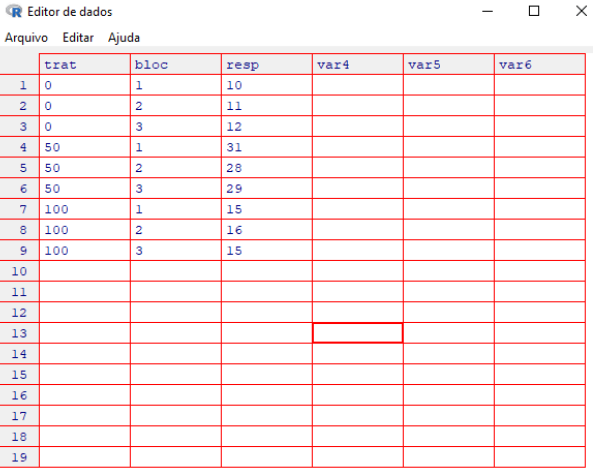
\includegraphics[width=8.26in]{image/scan1}

Se você precisar abrir novamente planilha com os dados, para fazer modificações e/ou inserir mais dados, use o comando \texttt{fix}:

\begin{Shaded}
\begin{Highlighting}[]
\KeywordTok{fix}\NormalTok{(dados)}
\KeywordTok{head}\NormalTok{(dados)}
\end{Highlighting}
\end{Shaded}

\hypertarget{exemplo-1}{%
\subsubsection{Exemplo 1}\label{exemplo-1}}

\begin{Shaded}
\begin{Highlighting}[]
\NormalTok{teste <-}\StringTok{ }\KeywordTok{c}\NormalTok{(}\DecValTok{10}\NormalTok{,}\DecValTok{20}\NormalTok{,}\DecValTok{30}\NormalTok{,}\DecValTok{40}\NormalTok{,}\DecValTok{50}\NormalTok{)}
\NormalTok{teste}
\end{Highlighting}
\end{Shaded}

\begin{verbatim}
## [1] 10 20 30 40 50
\end{verbatim}

Porém houve um erro: o último elemento deveria ser 60 e não 50, você não precisa criar novamente um objeto, use o comando \texttt{edit()}:

\begin{Shaded}
\begin{Highlighting}[]
\NormalTok{teste2 <-}\StringTok{ }\KeywordTok{edit}\NormalTok{(teste)}
\end{Highlighting}
\end{Shaded}

\begin{Shaded}
\begin{Highlighting}[]
\NormalTok{knitr}\OperatorTok{::}\KeywordTok{include_graphics}\NormalTok{(}\StringTok{"image/edit2.png"}\NormalTok{)}
\end{Highlighting}
\end{Shaded}

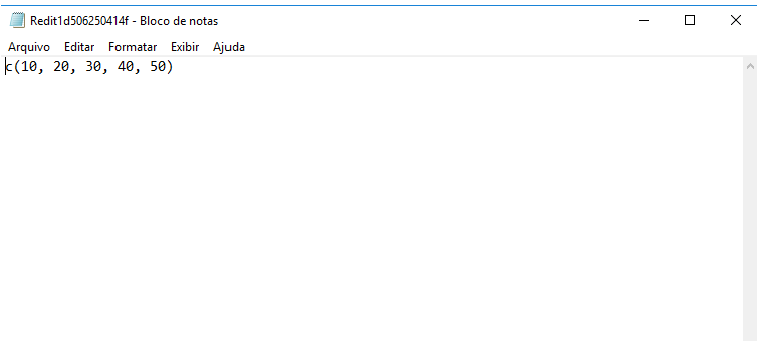
\includegraphics[width=10.54in]{image/edit2}

\hypertarget{exemplo-2}{%
\subsubsection{Exemplo 2}\label{exemplo-2}}

Com uma planilha com três colunas de dados. Os valores numéricos da coluna poderiam ser importados para o R utilizando-se o mesmo processo descrito com o uso do comando \texttt{scan()}. Abra o arquivo: \href{https://www.dropbox.com/s/6504oo4olw34dw9/EVI_Prec.xlsx?dl=1}{EVI-prec.xlsx}.

Uma matrix com os dados poderá ser obtida com o comando \texttt{cbind}:

\begin{Shaded}
\begin{Highlighting}[]
\NormalTok{dados <-}\StringTok{ }\KeywordTok{cbind}\NormalTok{(ano, chuva, evi)}
\end{Highlighting}
\end{Shaded}

O objeto dados é um \textbf{data.frame}:

\begin{Shaded}
\begin{Highlighting}[]
\KeywordTok{is.data.frame}\NormalTok{(dados)}
\end{Highlighting}
\end{Shaded}

Transforme para um data.frame com o comando \textbf{as.data.frame}:

\begin{Shaded}
\begin{Highlighting}[]
\NormalTok{dados_m <-}\StringTok{ }\KeywordTok{as.data.frame}\NormalTok{(dados)}
\end{Highlighting}
\end{Shaded}

Poderia usar o comando data.frame direto:

\begin{Shaded}
\begin{Highlighting}[]
\NormalTok{dados=}\KeywordTok{data.frame}\NormalTok{ (ano, chuva, evi)}
\end{Highlighting}
\end{Shaded}

\hypertarget{lendo-dados-de-um-arquivo-texto}{%
\subsection{Lendo dados de um arquivo texto}\label{lendo-dados-de-um-arquivo-texto}}

É muito importante ter os dados tabulados em um arquivo-texto ou em outros formatos que permitem a conversão para dados texto. O comando \texttt{read.table\ ()} é extremamente útil por ler dados de um arquivo-texto no formato de um \textbf{data.frame}

Usando o Comando \texttt{read.table\ ()}

\hypertarget{exemplo-1-1}{%
\subsubsection{Exemplo 1}\label{exemplo-1-1}}

Como primeiro exemplo considere importar para o R os dados do arquivo texto: \href{https://www.dropbox.com/s/m7jivbbggei5y0x/exemplo1.txt?dl=1}{exemplo1.txt}.

\begin{Shaded}
\begin{Highlighting}[]
\NormalTok{ex01 <-}\StringTok{ }\KeywordTok{read.table}\NormalTok{(}\StringTok{"exemplo1.txt"}\NormalTok{) }

\CommentTok{#Use os comandos}
\NormalTok{  ex01}
  \KeywordTok{class}\NormalTok{(ex01)}
  \KeywordTok{names}\NormalTok{(ex01)}
  \KeywordTok{dim}\NormalTok{(ex01)}
  \KeywordTok{str}\NormalTok{(ex01)}
  \KeywordTok{head}\NormalTok{(ex01)}
\end{Highlighting}
\end{Shaded}

\hypertarget{exemplo-2-1}{%
\subsubsection{Exemplo 2}\label{exemplo-2-1}}

Como primeiro exemplo considere importar para o R os dados do arquivo de texto: \href{https://www.dropbox.com/s/bi4b0j2nnnetc1r/exemplo2.txt?dl=1}{exemplo2.txt}.

\begin{Shaded}
\begin{Highlighting}[]
\NormalTok{ex02 <-}\StringTok{ }\KeywordTok{read.table}\NormalTok{(}\StringTok{"exemplo2.txt"}\NormalTok{) }
\NormalTok{ex02}
\end{Highlighting}
\end{Shaded}

Note que este arquivo difere do anterior em um aspecto: os nomes das variáveis estão na primeira linha. Para que o R considere isto corretamente, temos que informá-lo com o argumento \emph{head=T}. Portanto para importar este arquivo usamos:

\begin{Shaded}
\begin{Highlighting}[]
\NormalTok{ex02 <-}\StringTok{ }\KeywordTok{read.table}\NormalTok{(}\StringTok{"exemplo02.txt"}\NormalTok{, }\DataTypeTok{head=}\NormalTok{T) }
\NormalTok{ex02}
\end{Highlighting}
\end{Shaded}

\hypertarget{dados-do-tipo-csv}{%
\subsection{Dados do tipo CSV}\label{dados-do-tipo-csv}}

\href{https://www.dropbox.com/s/mv13cmkysw2nizm/exemplo3.csv?dl=1}{Exemplo3.csv}: Vamos utilizar um arquivo de tipo \textbf{CSV}:

\begin{Shaded}
\begin{Highlighting}[]
\NormalTok{ex03 <-}\StringTok{ }\KeywordTok{read.table}\NormalTok{(}\StringTok{"exemplo3.csv."}\NormalTok{, }\DataTypeTok{head=}\NormalTok{T, }\DataTypeTok{sep=}\StringTok{":"}\NormalTok{, }\DataTypeTok{dec=}\StringTok{","}\NormalTok{) }
\NormalTok{ex03}
\end{Highlighting}
\end{Shaded}

Note que este arquivo difere do primeiro em outros aspectos:
\emph{read.table.}

\begin{Shaded}
\begin{Highlighting}[]
\NormalTok{ex03 <-}\StringTok{ }\KeywordTok{read.table}\NormalTok{(       }\CommentTok{# lê dados de um arquivo texto}
  \StringTok{"exemplo3.csv"}\NormalTok{,         }\CommentTok{# nome do arquivo ou o caminho c:/R.exemplo3.csv}
  \DataTypeTok{head=}\NormalTok{T,                 }\CommentTok{# primeira linha ? cabe?alho}
  \DataTypeTok{sep=}\StringTok{":"}\NormalTok{,                }\CommentTok{# separador de coluna }
  \DataTypeTok{dec=}\StringTok{","}\NormalTok{)                }\CommentTok{# virgula como separador}
\NormalTok{ex03                      }\CommentTok{# exibe o objeto}
\end{Highlighting}
\end{Shaded}

1.\textbf{sep}: caractere utilizado para separação dos campos e valores. Normalmente é utilizado o ponto e virgula (;)

1.\textbf{dec}: caractere utilizado para separar as casas decimais. Normalmente ponto (.) ou virgula (,).

1.\textbf{header}: TRUE, assume que a primeira linha da tabela contêm rotulos das variáveis. `FALSE', assume que os dados se iniciam na primeira linha.

\hypertarget{a-seguir-listamos-algumas-destas-funuxe7uxf5es}{%
\subsection{A seguir listamos algumas destas funções:}\label{a-seguir-listamos-algumas-destas-funuxe7uxf5es}}

\begin{enumerate}
\def\labelenumi{\arabic{enumi}.}
\tightlist
\item
  \emph{read.dbf()} para arquivos DBASE
\item
  \emph{read.epiinfo()} para arquivos .REC do Epi-Info
\item
  \emph{read.mtp()} para arquivos ``Minitab Portable Worksheet''
\item
  \emph{read.S()} para arquivos do S-PLUS, e restore.data() para ``dumps'' do S-PLUS
\item
  \emph{read.spss()} para dados do SPSS
\item
  \emph{read.systat()} para dados do SYSTAT
\item
  \emph{read.dta()} para dados do STATA
\item
  \emph{read.octave()} para dados do OCTAVE (um clone do MATLAB)
\item
  \emph{read.csv}(file, header = TRUE, sep=``,'', dec=``.'')
\item
  \emph{read.csv2}(file, header = TRUE, sep=``;'', dec=``,'')
\item
  \emph{read.delim}(file, header = TRUE, sep=``\t", dec=''.")
\item
  \emph{read.delim2}(file, header = TRUE, sep=``\t", dec='',")
\end{enumerate}

\hypertarget{lendo-dados-disponuxedveis-na-web}{%
\subsection{Lendo dados disponíveis na web}\label{lendo-dados-disponuxedveis-na-web}}

\textbf{Exemplo 4}: As funções permitem ler ainda dados diretamente disponíveis na web. Por exemplo os dados do \href{https://www.dropbox.com/s/m7jivbbggei5y0x/exemplo1.txt?dl=1}{exemplo1.txt} poderiam ser lidos diretamente com o comando a seguir:

\hypertarget{lendo-dados-de-uma-planilha-eletruxf4nica}{%
\subsection{Lendo dados de uma planilha eletrônica}\label{lendo-dados-de-uma-planilha-eletruxf4nica}}

Com o \textbf{pacote xlsx} é possivel ler os dados diretamente da planilha eletrônica do Excel.

\begin{Shaded}
\begin{Highlighting}[]
\KeywordTok{install.packages}\NormalTok{(}\StringTok{""}\NormalTok{)}
\KeywordTok{require}\NormalTok{(}\StringTok{"xlsx"}\NormalTok{)}
\end{Highlighting}
\end{Shaded}

O comando \emph{read.xlsx()}, do \textbf{pacote xlsx}, lê o conteúdo de uma planilha eletrônica para o R com a estrutura de dados de um \emph{data.frame}:

\begin{Shaded}
\begin{Highlighting}[]
\NormalTok{dados <-}\StringTok{ }\KeywordTok{read.xlsx}\NormalTok{(}
                    \DataTypeTok{file=}\StringTok{"C:/R/EVI_Prec.xlsx"}\NormalTok{,     }\CommentTok{#comando que lê planilhas}
                    \DataTypeTok{sheetName =} \StringTok{"Conbea"}\NormalTok{,          }\CommentTok{#nome da planilha}
                    \DataTypeTok{h=}\NormalTok{T)                           }\CommentTok{#sem cabeçalho  }
\end{Highlighting}
\end{Shaded}

\hypertarget{exercuxedcios}{%
\subsection{Exercícios}\label{exercuxedcios}}

\begin{enumerate}
\def\labelenumi{\arabic{enumi}.}
\tightlist
\item
  Baixe os seguintes arquivos:

  \begin{itemize}
  \tightlist
  \item
    \href{https://www.dropbox.com/s/uq1n2sv8an2eoan/BanzattoQd1.2.3.txt?dl=1}{BanzattoQd1.2.3.txt}
  \item
    \href{https://www.dropbox.com/s/jjyo8dhyy0qt3ft/BanzattoQd3.2.1.txt?dl=1}{BanzattoQd3.2.1.txt}
  \item
    \href{https://www.dropbox.com/s/yv5clm6qljurzbw/BanzattoQd3.4.1.txt?dl=1}{BanzattoQd3.4.1.txt}
  \end{itemize}
\end{enumerate}

Coloque os arquivos em um local apropriado (de preferência no mesmo diretório de trabalho que você definiu no início da sessão), faça a importação usando a função de sua escolha, e confira a estrutura dos dados com ´str()´:

\hypertarget{salvar-objetos-de-dados}{%
\section{Salvar objetos de dados}\label{salvar-objetos-de-dados}}

Salvar objetos de dados nos formatos \textbf{.txt} ou \textbf{.csv}
função: \textbf{write.table}
sintaxe da função:
\emph{write.table}(x, file, sep="``, dec=''", rownames = T, col.names = T)

Principais argumentos:
1. x - matriz ou data frame
1. file - nome do arquivo ou caminho do arquivo
1. sep - separador da coluna
1. dec - separador deciminal

\hypertarget{outras-funuxe7uxf5es}{%
\subsection{Outras funções}\label{outras-funuxe7uxf5es}}

\texttt{write.csv()}
\texttt{write.csv2()}
\texttt{write.xlsx\ ()}

\textbf{Exemplo:}
write.xlsx(dados,``tabela salva.xlsx'')

\hypertarget{referuxeancia-2}{%
\section{Referência}\label{referuxeancia-2}}

MELO, M. P.; PETERNELI, L. A. \textbf{Conhecendo o R: Um visão mais que estatística}. Viçosa, MG: UFV, 2013. 222p.

\textbf{Prof.~Paulo Justiniando Ribeiro} \textgreater{}\url{http://www.leg.ufpr.br/~paulojus/}\textless{}

\textbf{Prof.~Adriano Azevedo Filho} \textgreater{}\url{http://rpubs.com/adriano/esalq2012inicial}\textless{}

\textbf{Prof.~Fernando de Pol Mayer} \textgreater{}\url{https://fernandomayer.github.io/ce083-2016-2/}\textless{}

\hypertarget{criando-gruxe1ficos-com-o-r}{%
\chapter{Criando Gráficos com o R}\label{criando-gruxe1ficos-com-o-r}}

Este capítulo foi baseado nos livros \href{https://www.editoraufv.com.br/produto/conhecendo-o-r-uma-visao-mais-que-estatistica/1109294}{\textbf{Conhecendo o R: Um visão mais que estatística}}.

AQUINO, J. A. \textbf{R para cientistas sociais}. - Ilhéus, BA: EDITUS, 2014. 157.

ANJOS, A. \textbf{Análise gráfica com uso do R}. Apostila. Dep. de Estatistica da UFPR, 2016. 127p.

Sites:

\url{https://www.statmethods.net/index.html}
\url{http://curso-r.github.io/index.html} PET Estatística UFPR (2016). \textbf{labestData: Biblioteca de Dados para Aprendizado de Estatística}. R package version x.y-z.w.
\url{https://www.statmethods.net/index.html}

O R é uma poderosa ferramenta no que diz respeito à confeção de gráficos. Iremos abordar três categorias de comandos gráficos, com o uso do pacote báscico do R o ``graphics''. Alguns pacotes foram desenvolvidos especialmente para manipulação de gráficos, como \emph{lattice}, \emph{ggplot2}, \emph{ggobi} e \emph{rgl}.

O R possui diferentes funções geradoras de gráficos, e essas são classificados como:

\begin{itemize}
\item
  \emph{Funções gráficas de alto nível}: criam novos gráficos na janela, definindo eixos, título, etc. Exemplos: \emph{plot, hist, image, contour, persp etc}.
\item
  \emph{Funções gráficas de baixo nível}: permitem adicionar novas informações em gráficos já criados, como novos dados, linhas etc. Exemplos: \emph{points, lines, abline,} \emph{polygon, legend etc}.
\item
  \emph{Funções gráficas iterativas}: permitem retirar ou adicionar informações aos gráficos já existentes, usando por exemplo o cursor do mouse. Exemplos: \emph{locator e identify}.
\end{itemize}

\hypertarget{exemplos-de-gruxe1ficos-com-o-r}{%
\section{Exemplos de gráficos com o R}\label{exemplos-de-gruxe1ficos-com-o-r}}

Você pode ver alguns exemplos de gráficos que podem ser criados no R com os seguintes comandos:

\begin{Shaded}
\begin{Highlighting}[]
\KeywordTok{demo}\NormalTok{(image)}
\end{Highlighting}
\end{Shaded}

\begin{verbatim}
## 
## 
##  demo(image)
##  ---- ~~~~~
## 
## > #  Copyright (C) 1997-2009 The R Core Team
## > 
## > require(datasets)
## 
## > require(grDevices); require(graphics)
## 
## > x <- 10*(1:nrow(volcano)); x.at <- seq(100, 800, by=100)
## 
## > y <- 10*(1:ncol(volcano)); y.at <- seq(100, 600, by=100)
## 
## >                    # Using Terrain Colors
## > 
## > image(x, y, volcano, col=terrain.colors(100),axes=FALSE)
\end{verbatim}

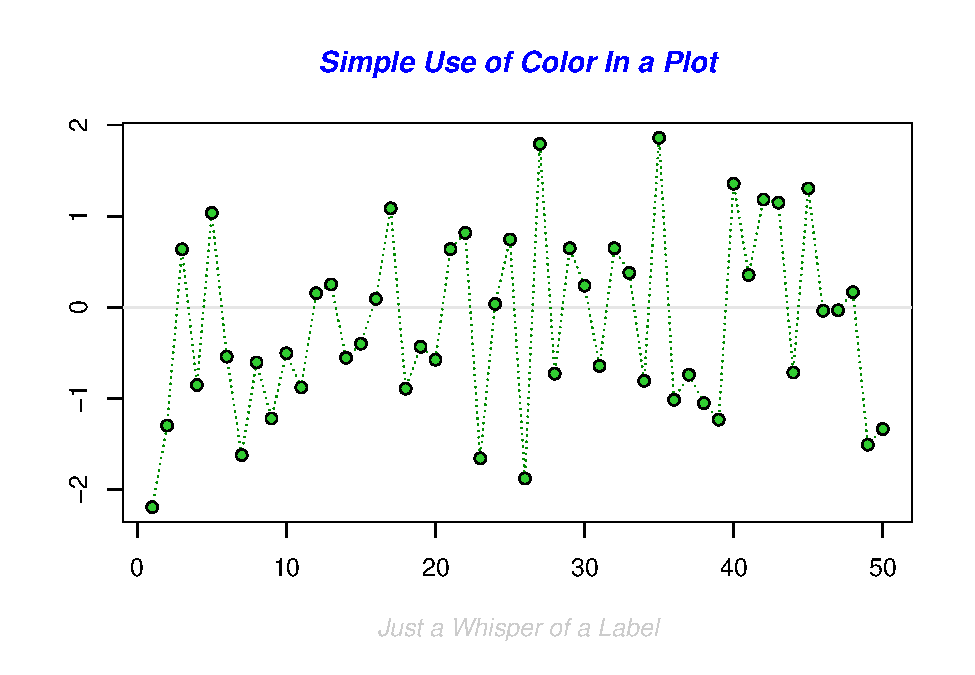
\includegraphics{TudodoR_files/figure-latex/unnamed-chunk-147-1.pdf}

\begin{verbatim}
## 
## > contour(x, y, volcano, levels=seq(90, 200, by=5), add=TRUE, col="brown")
## 
## > axis(1, at=x.at)
## 
## > axis(2, at=y.at)
## 
## > box()
## 
## > title(main="Maunga Whau Volcano", sub = "col=terrain.colors(100)", font.main=4)
## 
## >                    # Using Heat Colors
## > 
## > image(x, y, volcano, col=heat.colors(100), axes=FALSE)
\end{verbatim}

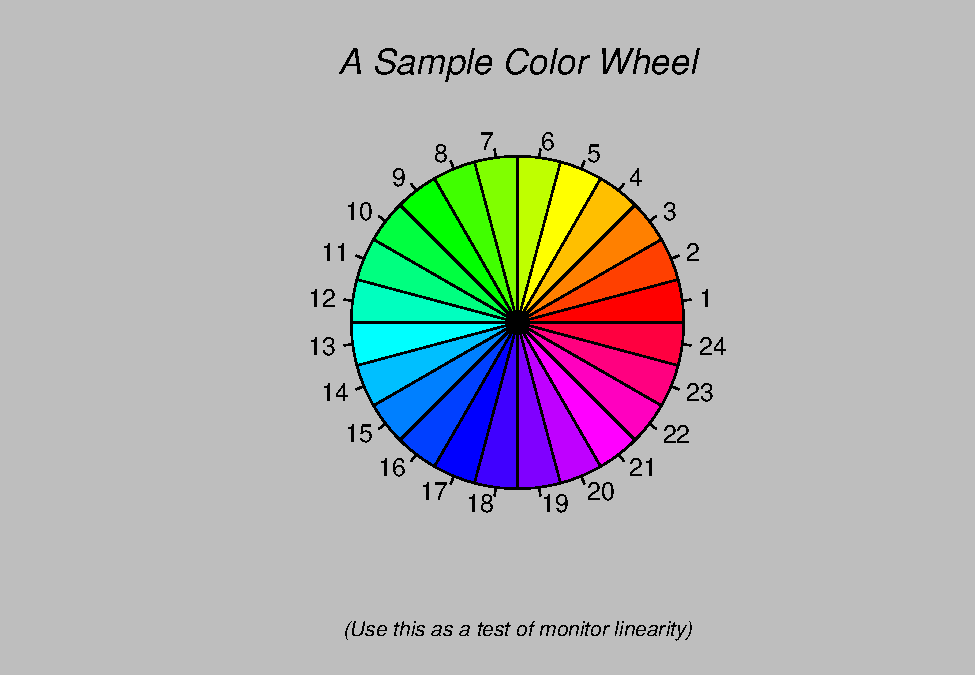
\includegraphics{TudodoR_files/figure-latex/unnamed-chunk-147-2.pdf}

\begin{verbatim}
## 
## > contour(x, y, volcano, levels=seq(90, 200, by=5), add=TRUE, col="brown")
## 
## > axis(1, at=x.at)
## 
## > axis(2, at=y.at)
## 
## > box()
## 
## > title(main="Maunga Whau Volcano", sub = "col=heat.colors(100)", font.main=4)
## 
## >                    # Using Gray Scale
## > 
## > image(x, y, volcano, col=gray(100:200/200), axes=FALSE)
\end{verbatim}

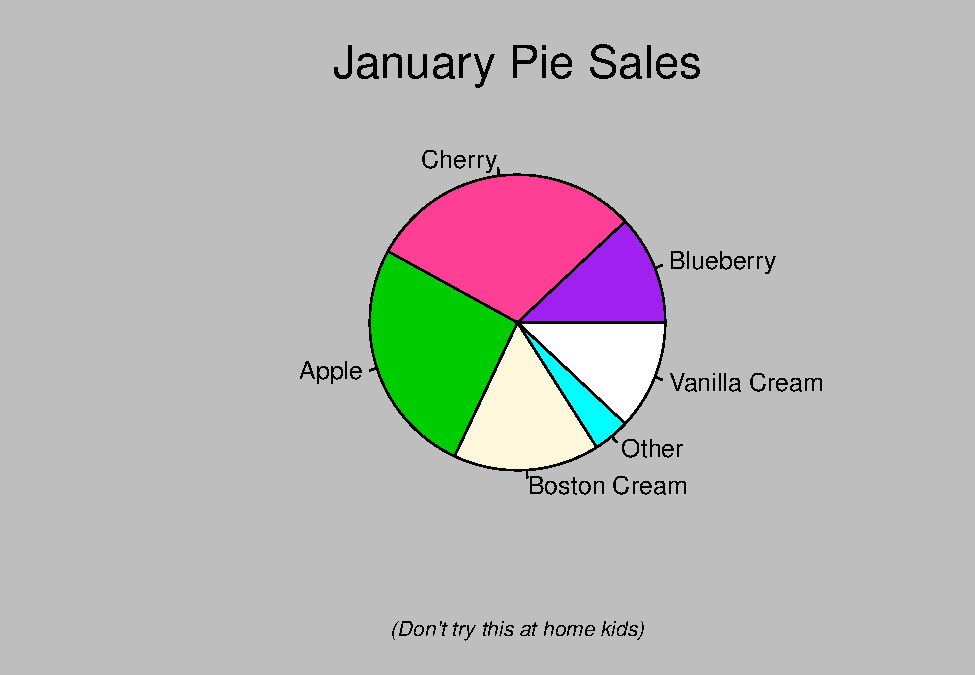
\includegraphics{TudodoR_files/figure-latex/unnamed-chunk-147-3.pdf}

\begin{verbatim}
## 
## > contour(x, y, volcano, levels=seq(90, 200, by=5), add=TRUE, col="black")
## 
## > axis(1, at=x.at)
## 
## > axis(2, at=y.at)
## 
## > box()
## 
## > title(main="Maunga Whau Volcano \n col=gray(100:200/200)", font.main=4)
## 
## > ## Filled Contours are even nicer sometimes :
## > example(filled.contour)
## 
## flld.c> require("grDevices") # for colours
## 
## flld.c> filled.contour(volcano, asp = 1) # simple
\end{verbatim}

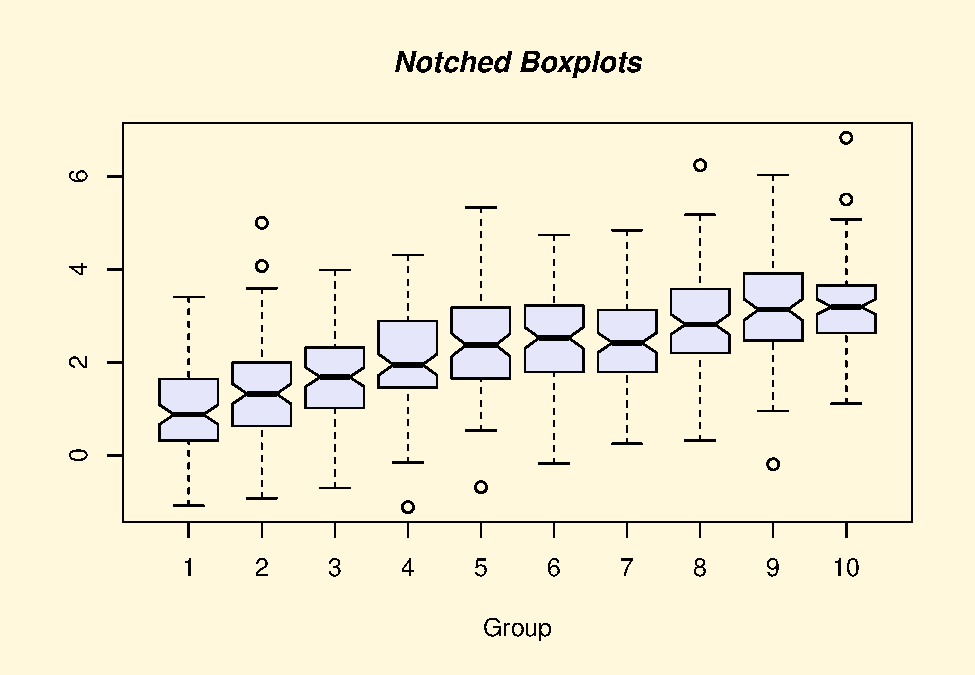
\includegraphics{TudodoR_files/figure-latex/unnamed-chunk-147-4.pdf}

\begin{verbatim}
## 
## flld.c> x <- 10*1:nrow(volcano)
## 
## flld.c> y <- 10*1:ncol(volcano)
## 
## flld.c> filled.contour(x, y, volcano, color = function(n) hcl.colors(n, "terrain"),
## flld.c+     plot.title = title(main = "The Topography of Maunga Whau",
## flld.c+     xlab = "Meters North", ylab = "Meters West"),
## flld.c+     plot.axes = { axis(1, seq(100, 800, by = 100))
## flld.c+                   axis(2, seq(100, 600, by = 100)) },
## flld.c+     key.title = title(main = "Height\n(meters)"),
## flld.c+     key.axes = axis(4, seq(90, 190, by = 10)))  # maybe also asp = 1
\end{verbatim}

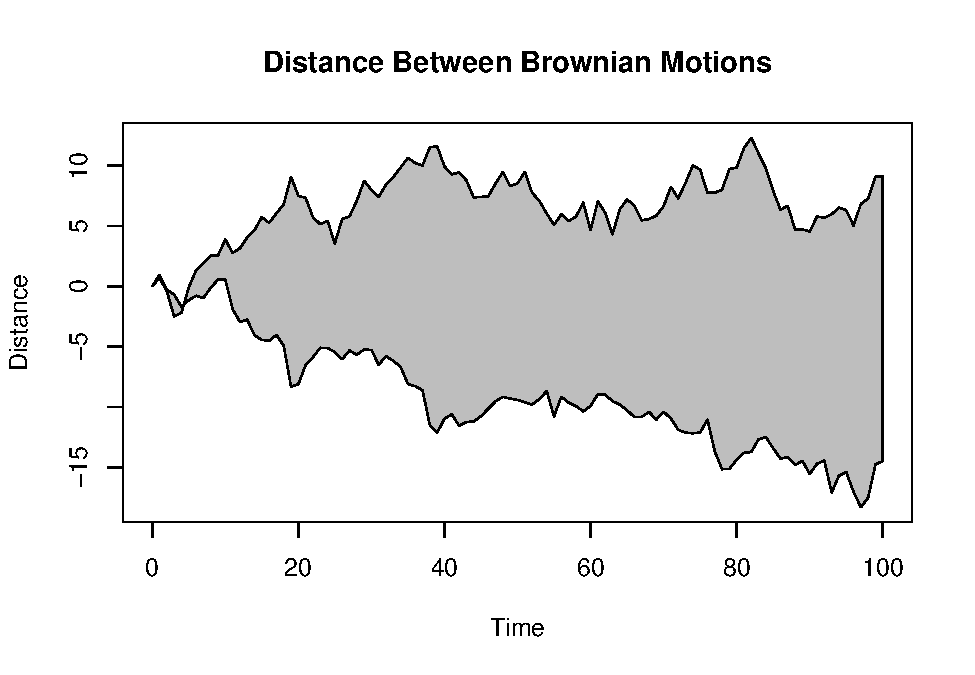
\includegraphics{TudodoR_files/figure-latex/unnamed-chunk-147-5.pdf}

\begin{verbatim}
## 
## flld.c> mtext(paste("filled.contour(.) from", R.version.string),
## flld.c+       side = 1, line = 4, adj = 1, cex = .66)
## 
## flld.c> # Annotating a filled contour plot
## flld.c> a <- expand.grid(1:20, 1:20)
## 
## flld.c> b <- matrix(a[,1] + a[,2], 20)
## 
## flld.c> filled.contour(x = 1:20, y = 1:20, z = b,
## flld.c+                plot.axes = { axis(1); axis(2); points(10, 10) })
\end{verbatim}

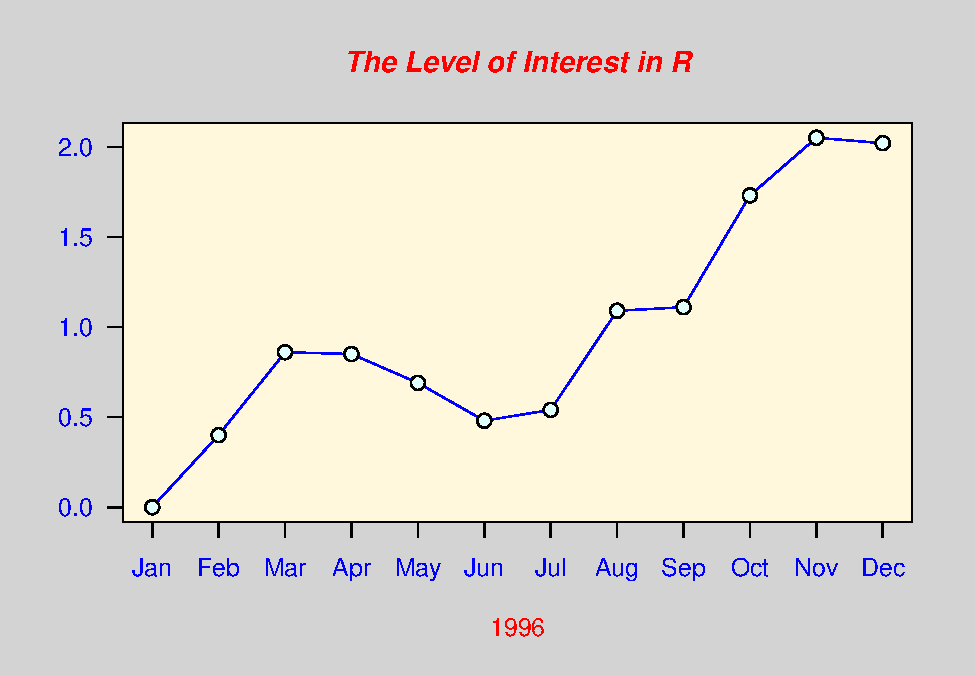
\includegraphics{TudodoR_files/figure-latex/unnamed-chunk-147-6.pdf}

\begin{verbatim}
## 
## flld.c> ## Persian Rug Art:
## flld.c> x <- y <- seq(-4*pi, 4*pi, len = 27)
## 
## flld.c> r <- sqrt(outer(x^2, y^2, "+"))
## 
## flld.c> filled.contour(cos(r^2)*exp(-r/(2*pi)), axes = FALSE)
\end{verbatim}

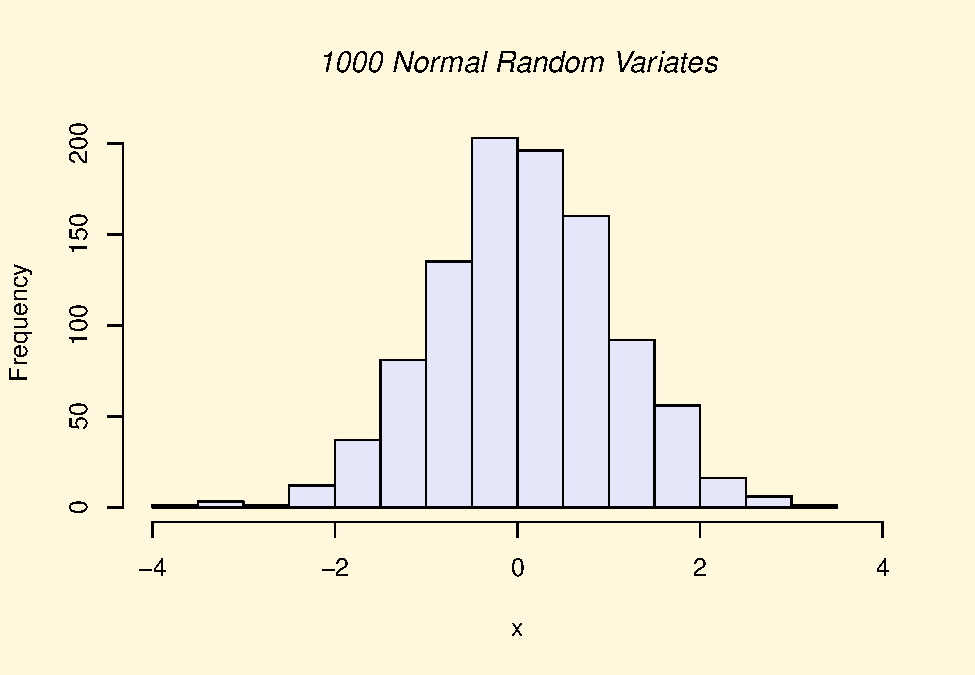
\includegraphics{TudodoR_files/figure-latex/unnamed-chunk-147-7.pdf}

\begin{verbatim}
## 
## flld.c> ## rather, the key *should* be labeled:
## flld.c> filled.contour(cos(r^2)*exp(-r/(2*pi)), frame.plot = FALSE,
## flld.c+                plot.axes = {})
\end{verbatim}

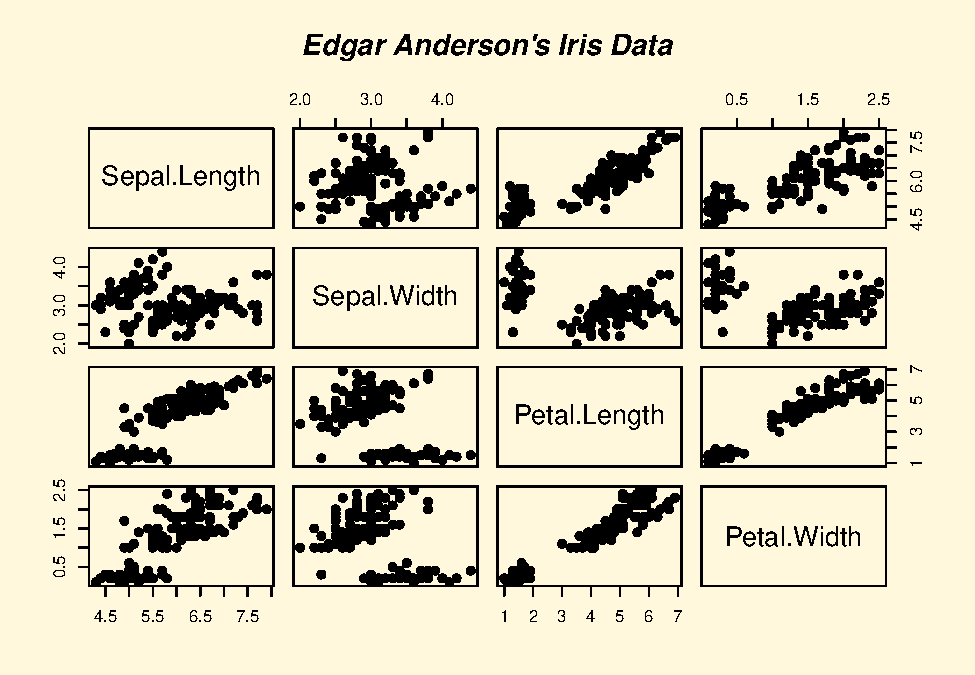
\includegraphics{TudodoR_files/figure-latex/unnamed-chunk-147-8.pdf}

\begin{Shaded}
\begin{Highlighting}[]
\KeywordTok{demo}\NormalTok{(persp)}
\end{Highlighting}
\end{Shaded}

\begin{verbatim}
## 
## 
##  demo(persp)
##  ---- ~~~~~
## 
## > ### Demos for  persp()  plots   -- things not in  example(persp)
## > ### -------------------------
## > 
## > require(datasets)
## 
## > require(grDevices); require(graphics)
## 
## > ## (1) The Obligatory Mathematical surface.
## > ##     Rotated sinc function.
## > 
## > x <- seq(-10, 10, length.out = 50)
## 
## > y <- x
## 
## > rotsinc <- function(x,y)
## + {
## +     sinc <- function(x) { y <- sin(x)/x ; y[is.na(y)] <- 1; y }
## +     10 * sinc( sqrt(x^2+y^2) )
## + }
## 
## > sinc.exp <- expression(z == Sinc(sqrt(x^2 + y^2)))
## 
## > z <- outer(x, y, rotsinc)
## 
## > oldpar <- par(bg = "white")
## 
## > persp(x, y, z, theta = 30, phi = 30, expand = 0.5, col = "lightblue")
\end{verbatim}

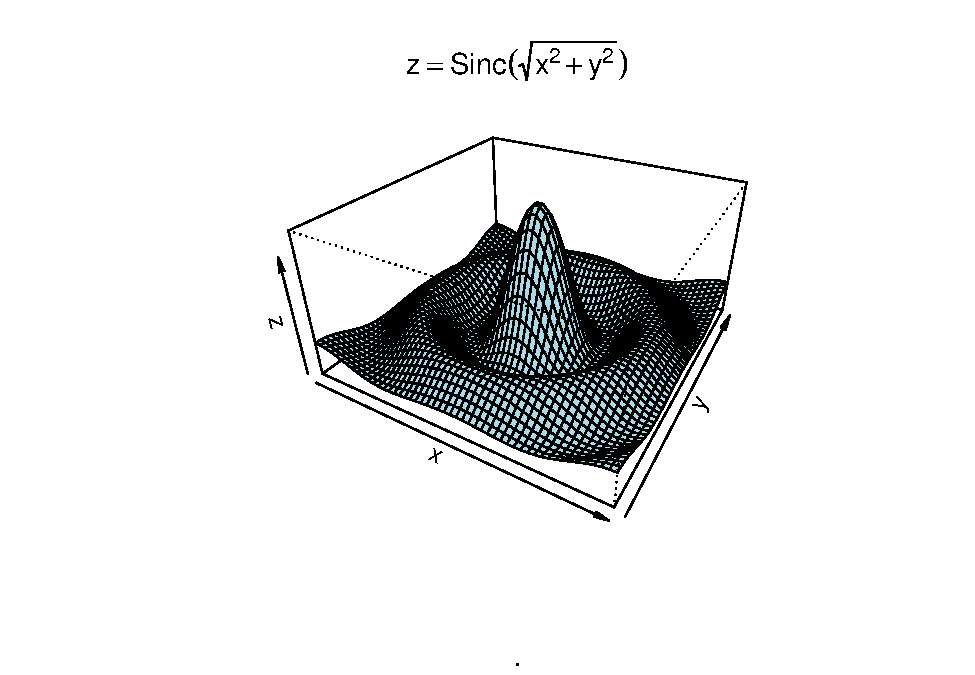
\includegraphics{TudodoR_files/figure-latex/unnamed-chunk-148-1.pdf}

\begin{verbatim}
## 
## > title(sub=".")## work around persp+plotmath bug
## 
## > title(main = sinc.exp)
## 
## > persp(x, y, z, theta = 30, phi = 30, expand = 0.5, col = "lightblue",
## +       ltheta = 120, shade = 0.75, ticktype = "detailed",
## +       xlab = "X", ylab = "Y", zlab = "Z")
\end{verbatim}

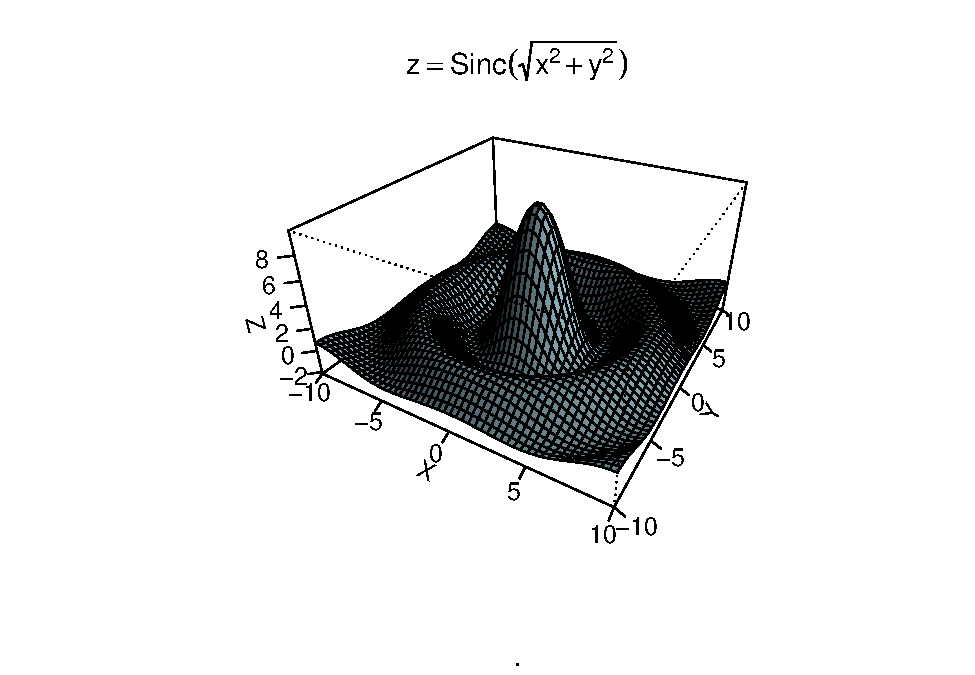
\includegraphics{TudodoR_files/figure-latex/unnamed-chunk-148-2.pdf}

\begin{verbatim}
## 
## > title(sub=".")## work around persp+plotmath bug
## 
## > title(main = sinc.exp)
## 
## > ## (2) Visualizing a simple DEM model
## > 
## > z <- 2 * volcano        # Exaggerate the relief
## 
## > x <- 10 * (1:nrow(z))   # 10 meter spacing (S to N)
## 
## > y <- 10 * (1:ncol(z))   # 10 meter spacing (E to W)
## 
## > persp(x, y, z, theta = 120, phi = 15, scale = FALSE, axes = FALSE)
\end{verbatim}

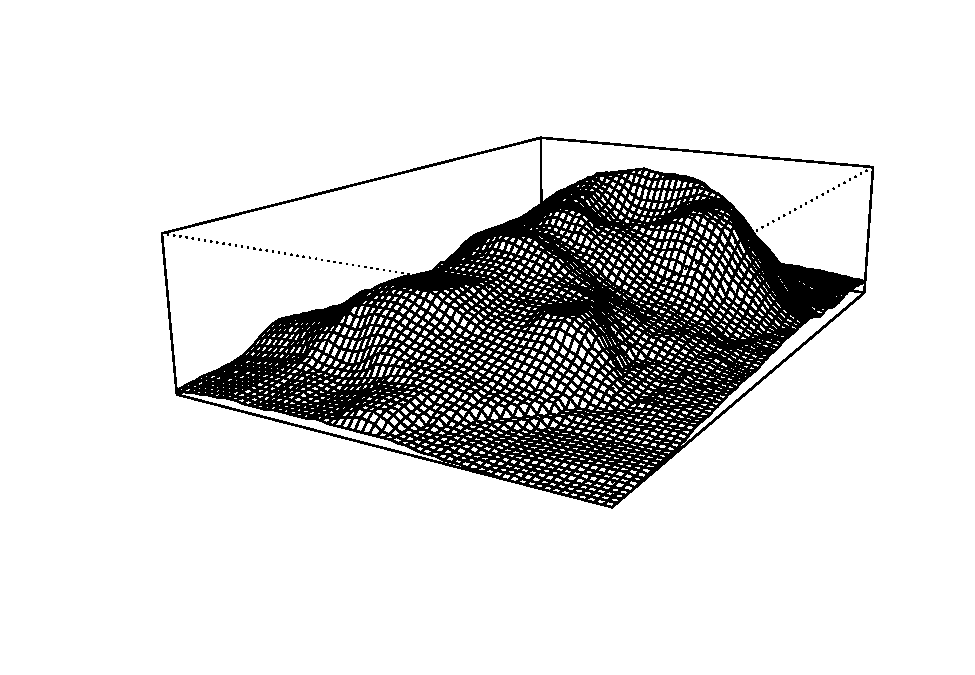
\includegraphics{TudodoR_files/figure-latex/unnamed-chunk-148-3.pdf}

\begin{verbatim}
## 
## > ## (3) Now something more complex
## > ##     We border the surface, to make it more "slice like"
## > ##     and color the top and sides of the surface differently.
## > 
## > z0 <- min(z) - 20
## 
## > z <- rbind(z0, cbind(z0, z, z0), z0)
## 
## > x <- c(min(x) - 1e-10, x, max(x) + 1e-10)
## 
## > y <- c(min(y) - 1e-10, y, max(y) + 1e-10)
## 
## > fill <- matrix("green3", nrow = nrow(z)-1, ncol = ncol(z)-1)
## 
## > fill[ , i2 <- c(1,ncol(fill))] <- "gray"
## 
## > fill[i1 <- c(1,nrow(fill)) , ] <- "gray"
## 
## > par(bg = "lightblue")
## 
## > persp(x, y, z, theta = 120, phi = 15, col = fill, scale = FALSE, axes = FALSE)
\end{verbatim}

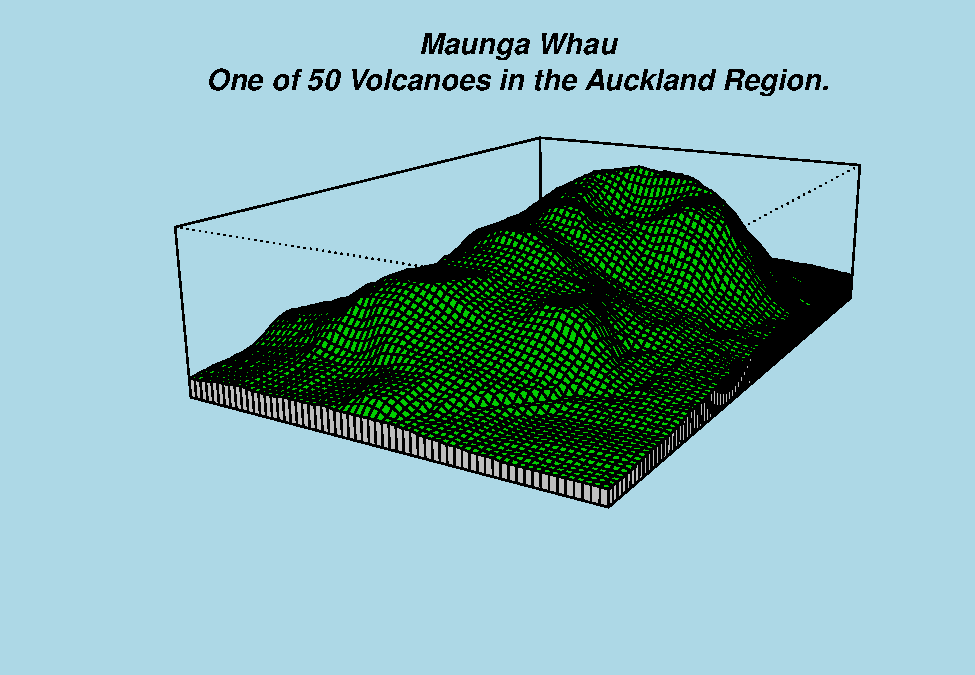
\includegraphics{TudodoR_files/figure-latex/unnamed-chunk-148-4.pdf}

\begin{verbatim}
## 
## > title(main = "Maunga Whau\nOne of 50 Volcanoes in the Auckland Region.",
## +       font.main = 4)
## 
## > par(bg = "slategray")
## 
## > persp(x, y, z, theta = 135, phi = 30, col = fill, scale = FALSE,
## +       ltheta = -120, lphi = 15, shade = 0.65, axes = FALSE)
\end{verbatim}

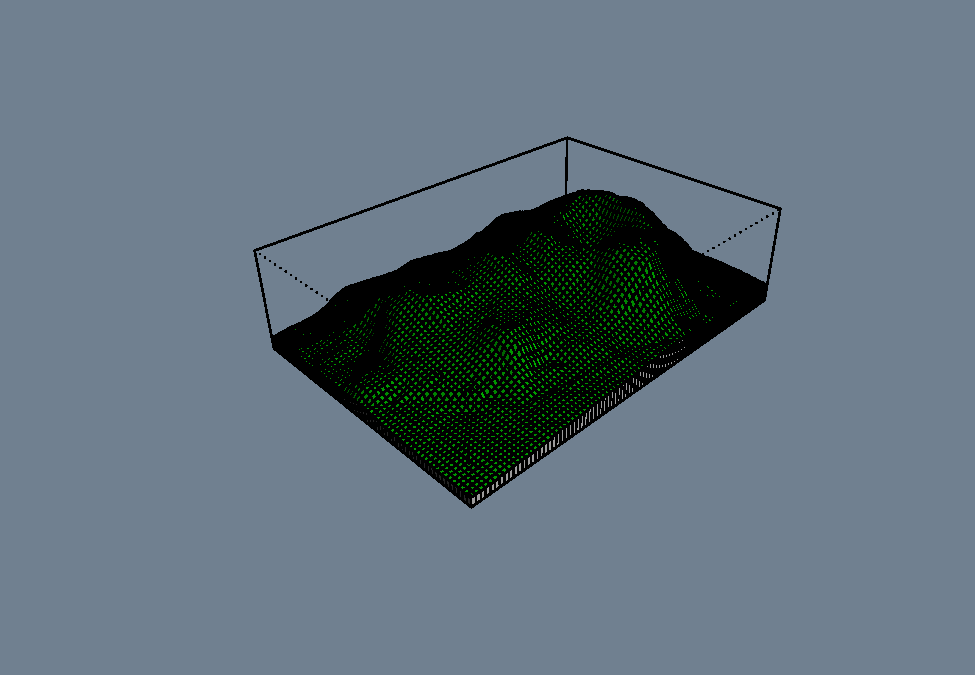
\includegraphics{TudodoR_files/figure-latex/unnamed-chunk-148-5.pdf}

\begin{verbatim}
## 
## > ## Don't draw the grid lines :  border = NA
## > persp(x, y, z, theta = 135, phi = 30, col = "green3", scale = FALSE,
## +       ltheta = -120, shade = 0.75, border = NA, box = FALSE)
\end{verbatim}

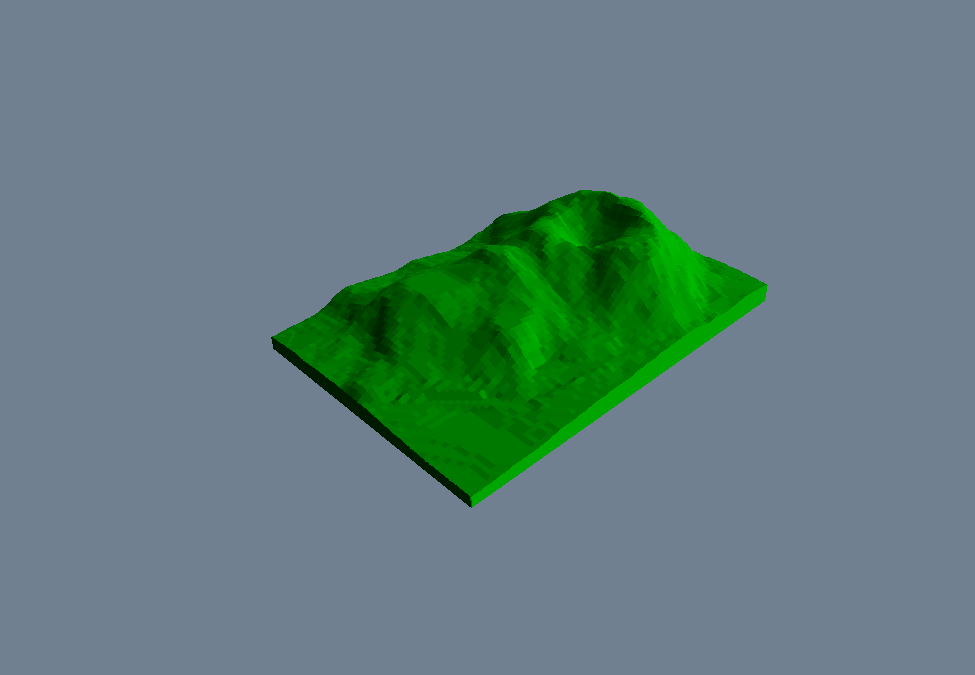
\includegraphics{TudodoR_files/figure-latex/unnamed-chunk-148-6.pdf}

\begin{verbatim}
## 
## > ## `color gradient in the soil' :
## > fcol <- fill ; fcol[] <- terrain.colors(nrow(fcol))
## 
## > persp(x, y, z, theta = 135, phi = 30, col = fcol, scale = FALSE,
## +       ltheta = -120, shade = 0.3, border = NA, box = FALSE)
\end{verbatim}

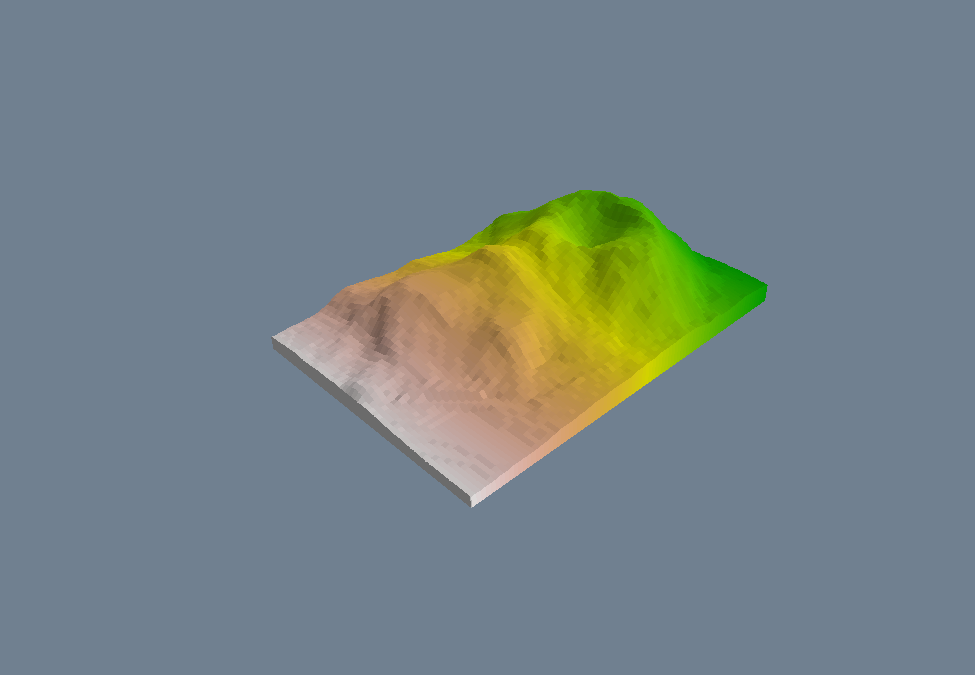
\includegraphics{TudodoR_files/figure-latex/unnamed-chunk-148-7.pdf}

\begin{verbatim}
## 
## > ## `image like' colors on top :
## > fcol <- fill
## 
## > zi <- volcano[ -1,-1] + volcano[ -1,-61] +
## +            volcano[-87,-1] + volcano[-87,-61]  ## / 4
## 
## > fcol[-i1,-i2] <-
## +     terrain.colors(20)[cut(zi,
## +                            stats::quantile(zi, seq(0,1, length.out = 21)),
## +                            include.lowest = TRUE)]
## 
## > persp(x, y, 2*z, theta = 110, phi = 40, col = fcol, scale = FALSE,
## +       ltheta = -120, shade = 0.4, border = NA, box = FALSE)
\end{verbatim}

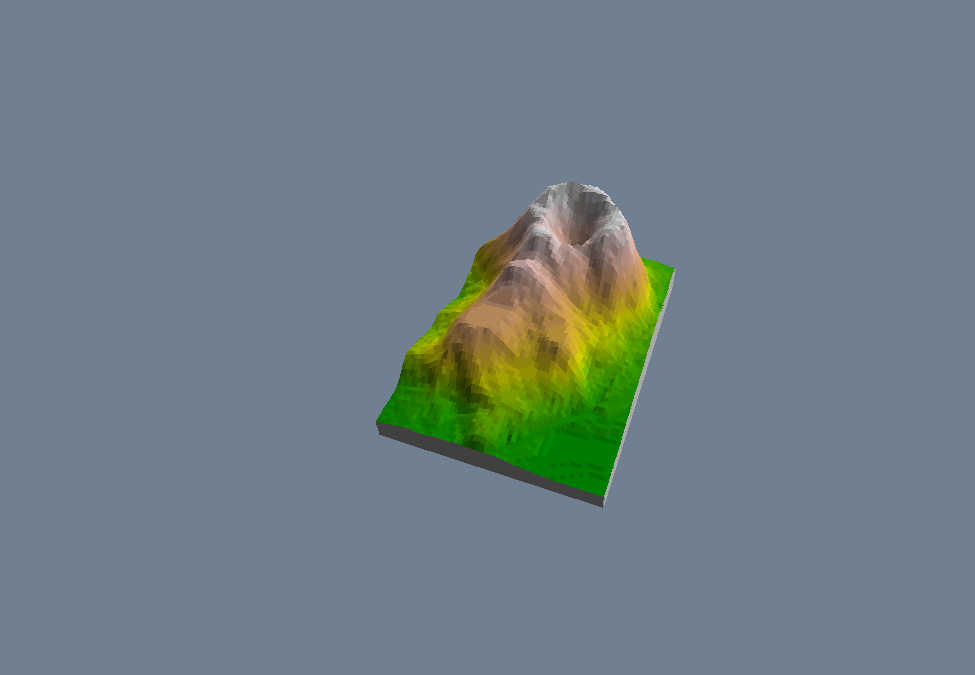
\includegraphics{TudodoR_files/figure-latex/unnamed-chunk-148-8.pdf}

\begin{verbatim}
## 
## > ## reset par():
## > par(oldpar)
\end{verbatim}

\begin{Shaded}
\begin{Highlighting}[]
\KeywordTok{demo}\NormalTok{(graphics)}
\end{Highlighting}
\end{Shaded}

\begin{verbatim}
## 
## 
##  demo(graphics)
##  ---- ~~~~~~~~
## 
## > #  Copyright (C) 1997-2009 The R Core Team
## > 
## > require(datasets)
## 
## > require(grDevices); require(graphics)
## 
## > ## Here is some code which illustrates some of the differences between
## > ## R and S graphics capabilities.  Note that colors are generally specified
## > ## by a character string name (taken from the X11 rgb.txt file) and that line
## > ## textures are given similarly.  The parameter "bg" sets the background
## > ## parameter for the plot and there is also an "fg" parameter which sets
## > ## the foreground color.
## > 
## > 
## > x <- stats::rnorm(50)
## 
## > opar <- par(bg = "white")
## 
## > plot(x, ann = FALSE, type = "n")
\end{verbatim}

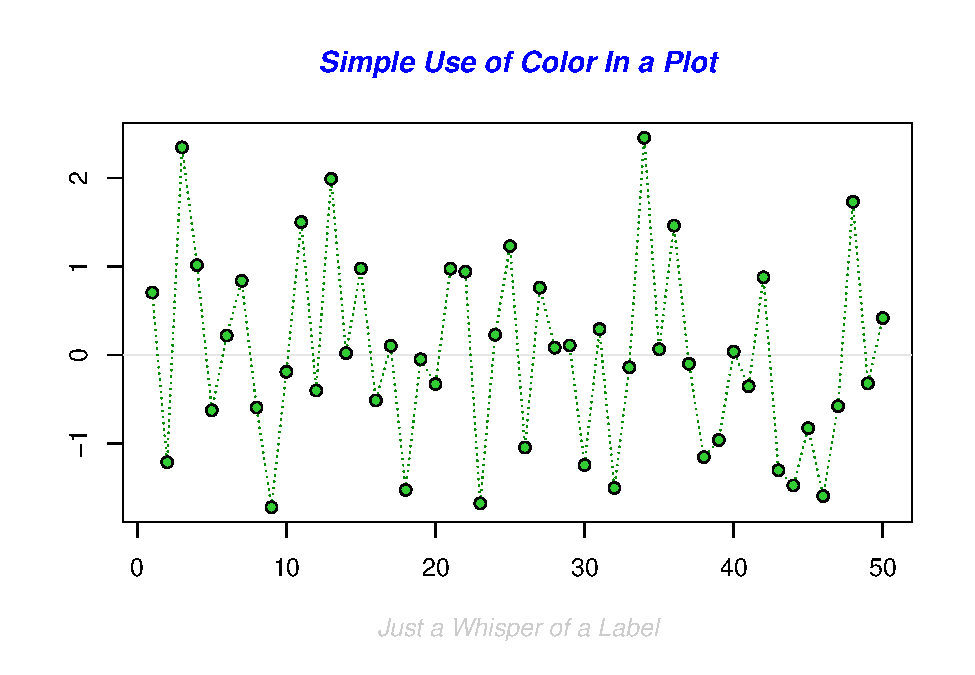
\includegraphics{TudodoR_files/figure-latex/unnamed-chunk-149-1.pdf}

\begin{verbatim}
## 
## > abline(h = 0, col = gray(.90))
## 
## > lines(x, col = "green4", lty = "dotted")
## 
## > points(x, bg = "limegreen", pch = 21)
## 
## > title(main = "Simple Use of Color In a Plot",
## +       xlab = "Just a Whisper of a Label",
## +       col.main = "blue", col.lab = gray(.8),
## +       cex.main = 1.2, cex.lab = 1.0, font.main = 4, font.lab = 3)
## 
## > ## A little color wheel.    This code just plots equally spaced hues in
## > ## a pie chart.    If you have a cheap SVGA monitor (like me) you will
## > ## probably find that numerically equispaced does not mean visually
## > ## equispaced.  On my display at home, these colors tend to cluster at
## > ## the RGB primaries.  On the other hand on the SGI Indy at work the
## > ## effect is near perfect.
## > 
## > par(bg = "gray")
## 
## > pie(rep(1,24), col = rainbow(24), radius = 0.9)
\end{verbatim}

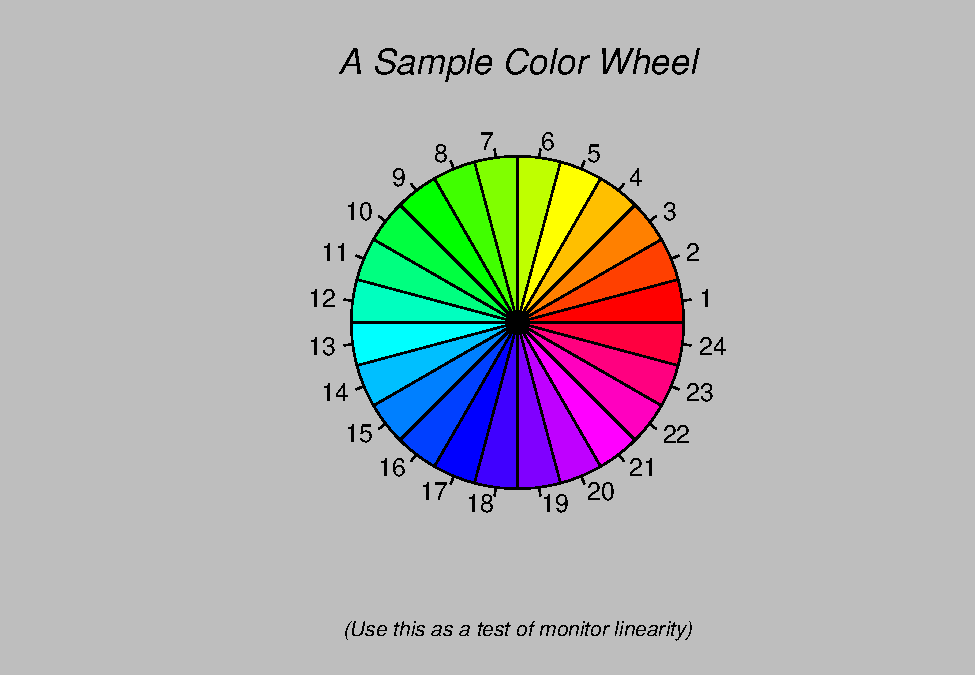
\includegraphics{TudodoR_files/figure-latex/unnamed-chunk-149-2.pdf}

\begin{verbatim}
## 
## > title(main = "A Sample Color Wheel", cex.main = 1.4, font.main = 3)
## 
## > title(xlab = "(Use this as a test of monitor linearity)",
## +       cex.lab = 0.8, font.lab = 3)
## 
## > ## We have already confessed to having these.  This is just showing off X11
## > ## color names (and the example (from the postscript manual) is pretty "cute".
## > 
## > pie.sales <- c(0.12, 0.3, 0.26, 0.16, 0.04, 0.12)
## 
## > names(pie.sales) <- c("Blueberry", "Cherry",
## +              "Apple", "Boston Cream", "Other", "Vanilla Cream")
## 
## > pie(pie.sales,
## +     col = c("purple","violetred1","green3","cornsilk","cyan","white"))
\end{verbatim}

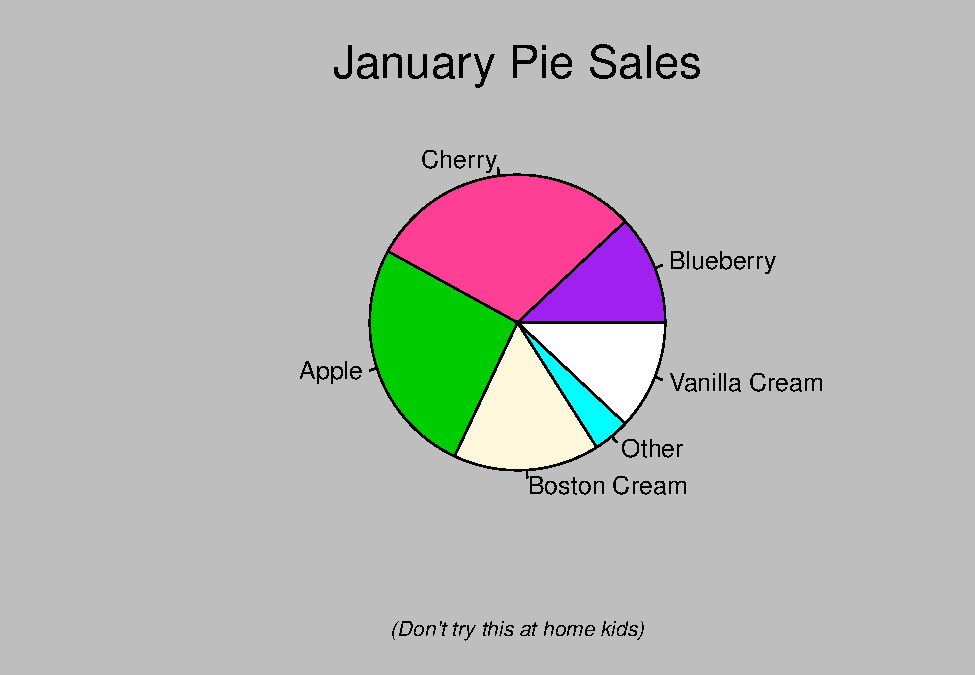
\includegraphics{TudodoR_files/figure-latex/unnamed-chunk-149-3.pdf}

\begin{verbatim}
## 
## > title(main = "January Pie Sales", cex.main = 1.8, font.main = 1)
## 
## > title(xlab = "(Don't try this at home kids)", cex.lab = 0.8, font.lab = 3)
## 
## > ## Boxplots:  I couldn't resist the capability for filling the "box".
## > ## The use of color seems like a useful addition, it focuses attention
## > ## on the central bulk of the data.
## > 
## > par(bg="cornsilk")
## 
## > n <- 10
## 
## > g <- gl(n, 100, n*100)
## 
## > x <- rnorm(n*100) + sqrt(as.numeric(g))
## 
## > boxplot(split(x,g), col="lavender", notch=TRUE)
\end{verbatim}

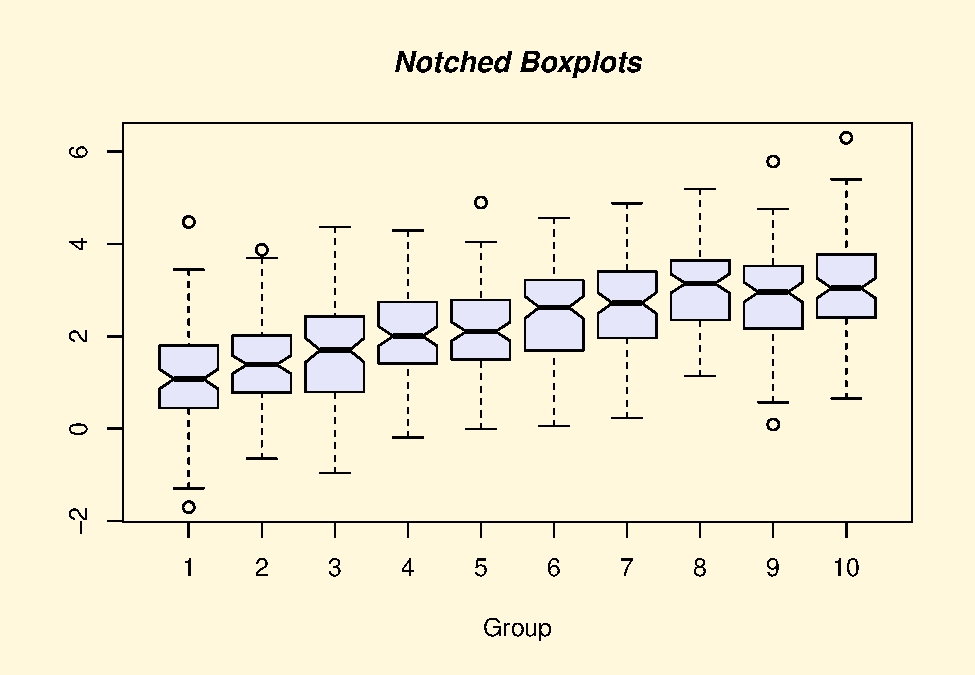
\includegraphics{TudodoR_files/figure-latex/unnamed-chunk-149-4.pdf}

\begin{verbatim}
## 
## > title(main="Notched Boxplots", xlab="Group", font.main=4, font.lab=1)
## 
## > ## An example showing how to fill between curves.
## > 
## > par(bg="white")
## 
## > n <- 100
## 
## > x <- c(0,cumsum(rnorm(n)))
## 
## > y <- c(0,cumsum(rnorm(n)))
## 
## > xx <- c(0:n, n:0)
## 
## > yy <- c(x, rev(y))
## 
## > plot(xx, yy, type="n", xlab="Time", ylab="Distance")
\end{verbatim}

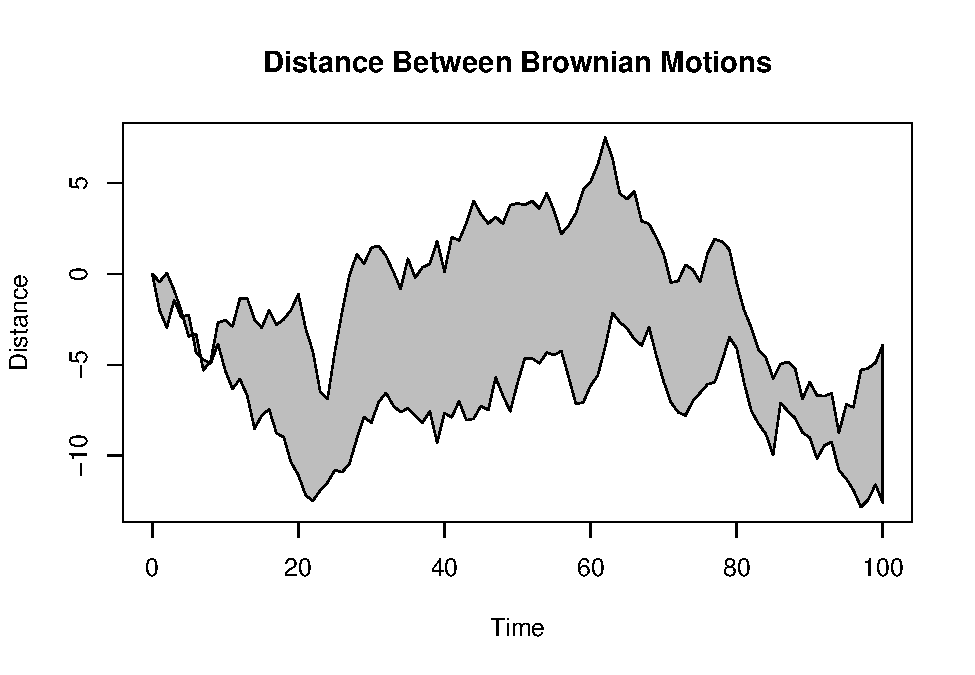
\includegraphics{TudodoR_files/figure-latex/unnamed-chunk-149-5.pdf}

\begin{verbatim}
## 
## > polygon(xx, yy, col="gray")
## 
## > title("Distance Between Brownian Motions")
## 
## > ## Colored plot margins, axis labels and titles.    You do need to be
## > ## careful with these kinds of effects.    It's easy to go completely
## > ## over the top and you can end up with your lunch all over the keyboard.
## > ## On the other hand, my market research clients love it.
## > 
## > x <- c(0.00, 0.40, 0.86, 0.85, 0.69, 0.48, 0.54, 1.09, 1.11, 1.73, 2.05, 2.02)
## 
## > par(bg="lightgray")
## 
## > plot(x, type="n", axes=FALSE, ann=FALSE)
\end{verbatim}

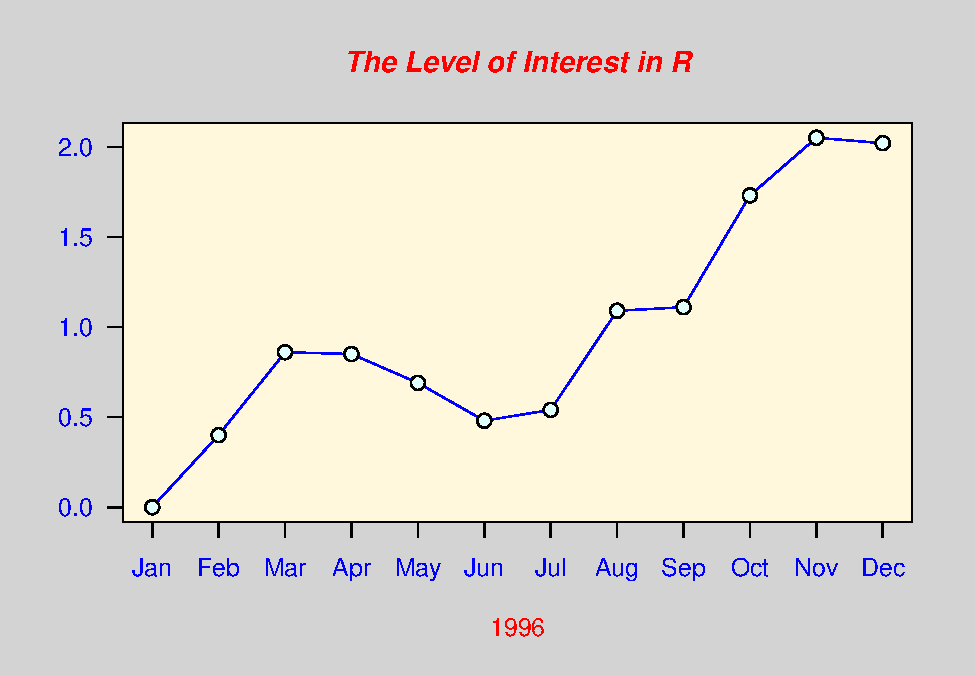
\includegraphics{TudodoR_files/figure-latex/unnamed-chunk-149-6.pdf}

\begin{verbatim}
## 
## > usr <- par("usr")
## 
## > rect(usr[1], usr[3], usr[2], usr[4], col="cornsilk", border="black")
## 
## > lines(x, col="blue")
## 
## > points(x, pch=21, bg="lightcyan", cex=1.25)
## 
## > axis(2, col.axis="blue", las=1)
## 
## > axis(1, at=1:12, lab=month.abb, col.axis="blue")
## 
## > box()
## 
## > title(main= "The Level of Interest in R", font.main=4, col.main="red")
## 
## > title(xlab= "1996", col.lab="red")
## 
## > ## A filled histogram, showing how to change the font used for the
## > ## main title without changing the other annotation.
## > 
## > par(bg="cornsilk")
## 
## > x <- rnorm(1000)
## 
## > hist(x, xlim=range(-4, 4, x), col="lavender", main="")
\end{verbatim}

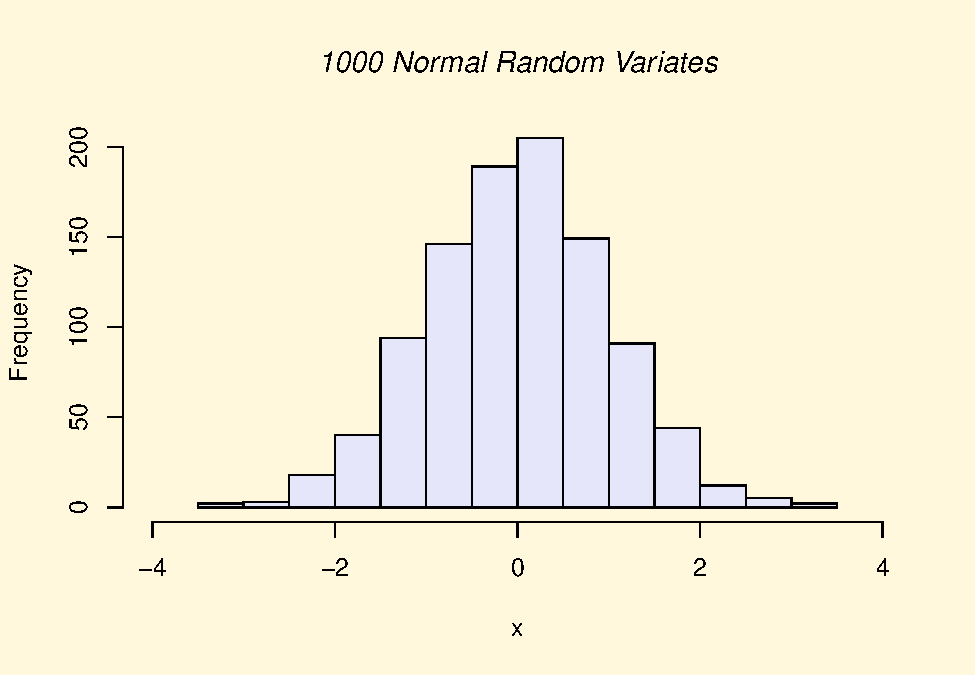
\includegraphics{TudodoR_files/figure-latex/unnamed-chunk-149-7.pdf}

\begin{verbatim}
## 
## > title(main="1000 Normal Random Variates", font.main=3)
## 
## > ## A scatterplot matrix
## > ## The good old Iris data (yet again)
## > 
## > pairs(iris[1:4], main="Edgar Anderson's Iris Data", font.main=4, pch=19)
\end{verbatim}

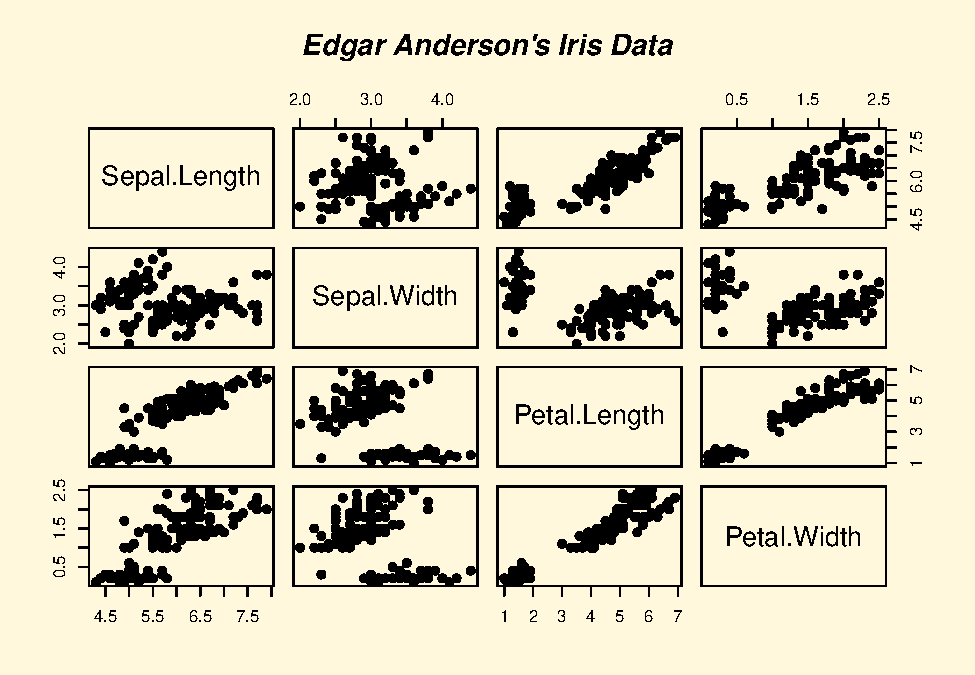
\includegraphics{TudodoR_files/figure-latex/unnamed-chunk-149-8.pdf}

\begin{verbatim}
## 
## > pairs(iris[1:4], main="Edgar Anderson's Iris Data", pch=21,
## +       bg = c("red", "green3", "blue")[unclass(iris$Species)])
\end{verbatim}

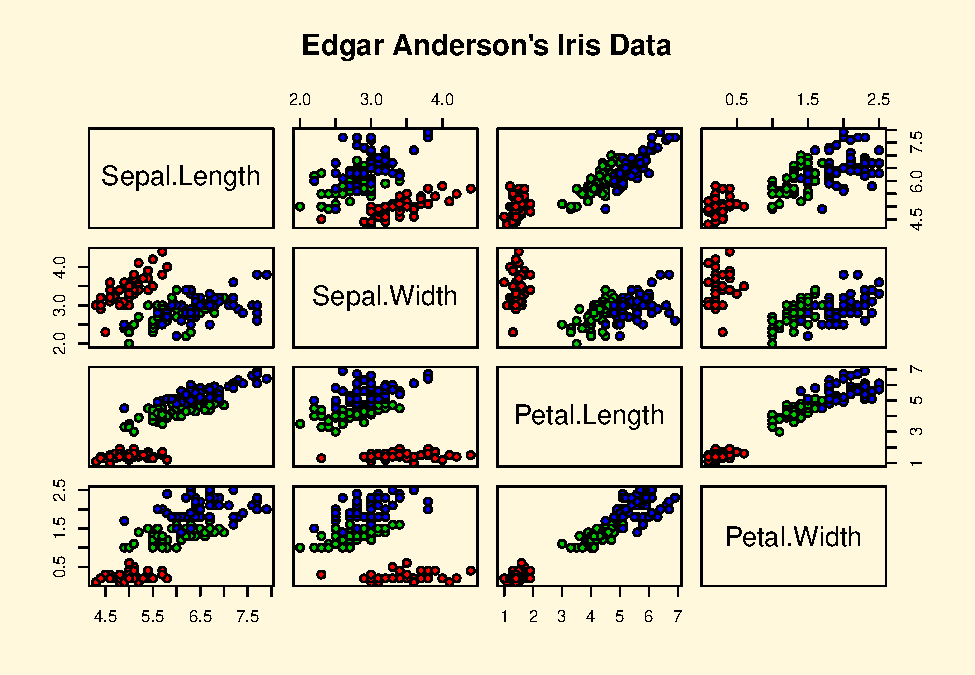
\includegraphics{TudodoR_files/figure-latex/unnamed-chunk-149-9.pdf}

\begin{verbatim}
## 
## > ## Contour plotting
## > ## This produces a topographic map of one of Auckland's many volcanic "peaks".
## > 
## > x <- 10*1:nrow(volcano)
## 
## > y <- 10*1:ncol(volcano)
## 
## > lev <- pretty(range(volcano), 10)
## 
## > par(bg = "lightcyan")
## 
## > pin <- par("pin")
## 
## > xdelta <- diff(range(x))
## 
## > ydelta <- diff(range(y))
## 
## > xscale <- pin[1]/xdelta
## 
## > yscale <- pin[2]/ydelta
## 
## > scale <- min(xscale, yscale)
## 
## > xadd <- 0.5*(pin[1]/scale - xdelta)
## 
## > yadd <- 0.5*(pin[2]/scale - ydelta)
## 
## > plot(numeric(0), numeric(0),
## +      xlim = range(x)+c(-1,1)*xadd, ylim = range(y)+c(-1,1)*yadd,
## +      type = "n", ann = FALSE)
\end{verbatim}

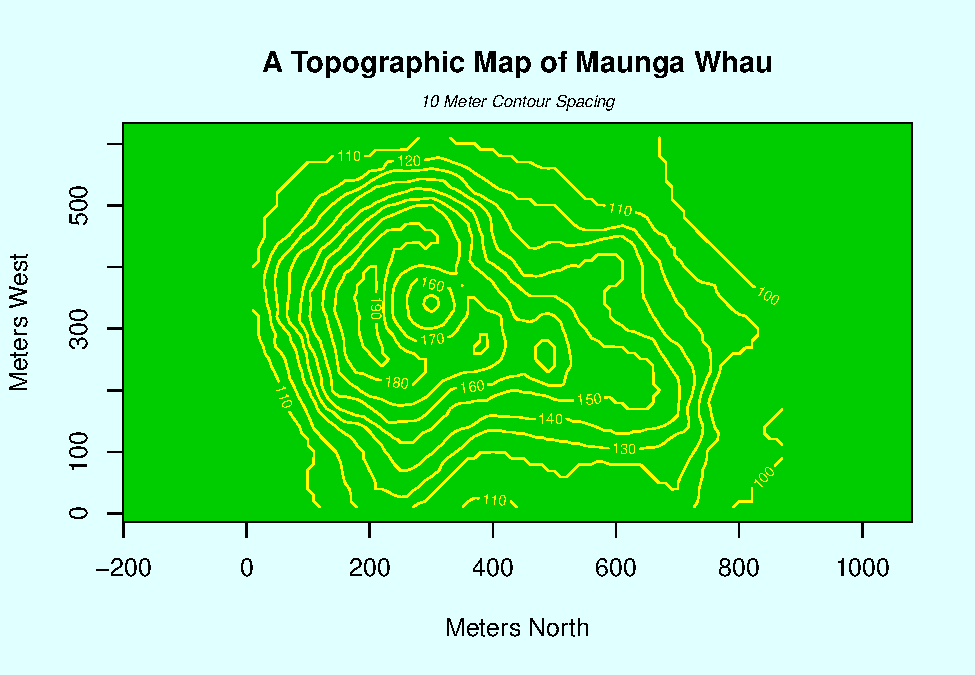
\includegraphics{TudodoR_files/figure-latex/unnamed-chunk-149-10.pdf}

\begin{verbatim}
## 
## > usr <- par("usr")
## 
## > rect(usr[1], usr[3], usr[2], usr[4], col="green3")
## 
## > contour(x, y, volcano, levels = lev, col="yellow", lty="solid", add=TRUE)
## 
## > box()
## 
## > title("A Topographic Map of Maunga Whau", font= 4)
## 
## > title(xlab = "Meters North", ylab = "Meters West", font= 3)
## 
## > mtext("10 Meter Contour Spacing", side=3, line=0.35, outer=FALSE,
## +       at = mean(par("usr")[1:2]), cex=0.7, font=3)
## 
## > ## Conditioning plots
## > 
## > par(bg="cornsilk")
## 
## > coplot(lat ~ long | depth, data = quakes, pch = 21, bg = "green3")
\end{verbatim}

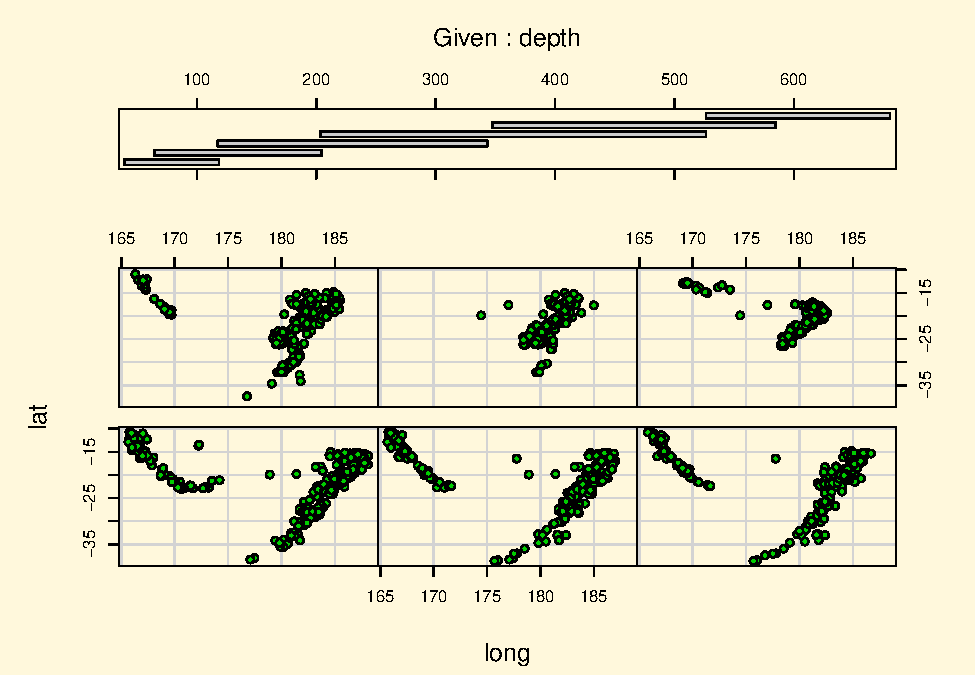
\includegraphics{TudodoR_files/figure-latex/unnamed-chunk-149-11.pdf}

\begin{verbatim}
## 
## > par(opar)
\end{verbatim}

\hypertarget{entrada-de-dados-1}{%
\section{Entrada de dados}\label{entrada-de-dados-1}}

Nesse tópico utlizaremos o arquivo de dados: \href{https://www.dropbox.com/s/zg7fyg1iewtji49/dadosfisio.csv?dl=1}{dadosfisio.csv}.

Dados físico hídrico de 3 solos com textutas diferentes:

\begin{longtable}[]{@{}lllll@{}}
\toprule
Cod. & Solo & Areia & Silte & Argila\tabularnewline
\midrule
\endhead
Z1 & NITOSSOLO & 122 & 121 & 757\tabularnewline
Z2 & LATOSSOLO & 710 & 80 & 210\tabularnewline
Z3 & LATOSSOLO & 892 & 10 & 98\tabularnewline
\bottomrule
\end{longtable}

Ler dados via web:

\begin{Shaded}
\begin{Highlighting}[]
\NormalTok{solo <-}\StringTok{ }\KeywordTok{read.table}\NormalTok{(}\StringTok{"https://www.dropbox.com/s/zg7fyg1iewtji49/dadosfisio.csv?dl=1"}\NormalTok{, }\DataTypeTok{sep =} \StringTok{";"}\NormalTok{, }\DataTypeTok{header =}\NormalTok{ T, }\DataTypeTok{dec =} \StringTok{","}\NormalTok{)}
\end{Highlighting}
\end{Shaded}

Verificar a estrutura de dados:

\begin{Shaded}
\begin{Highlighting}[]
\KeywordTok{str}\NormalTok{(solo)}
\end{Highlighting}
\end{Shaded}

\begin{verbatim}
## 'data.frame':    108 obs. of  16 variables:
##  $ z     : int  1 1 1 1 1 1 1 1 1 1 ...
##  $ x     : int  1 1 1 1 1 1 3 3 3 3 ...
##  $ y     : int  1 3 5 7 9 11 1 3 5 7 ...
##  $ cota  : num  9.15 8.95 8.78 8.59 8.48 8.41 8.93 8.76 8.58 8.48 ...
##  $ ds    : num  1.5 1.47 1.47 1.39 1.38 ...
##  $ cc    : num  0.398 0.382 0.351 0.372 0.356 ...
##  $ ma    : num  0.129 0.153 0.185 0.188 0.208 ...
##  $ ptotal: num  0.526 0.535 0.537 0.561 0.564 ...
##  $ tibo  : num  46.1 19.2 172.8 96 30.7 ...
##  $ tibe  : num  26.8 26.1 113.9 74.8 37.2 ...
##  $ a     : num  926 384 275 1207 151 ...
##  $ b     : num  -0.529 -0.418 -0.131 -0.376 -0.227 ...
##  $ X3    : num  518 243 238 798 118 ...
##  $ X60   : num  153.2 92.7 176.5 335.4 69.9 ...
##  $ X90   : num  106.2 69.4 161.2 258.4 59.8 ...
##  $ X120  : num  73.6 52 147.2 199 51.1 ...
\end{verbatim}

Resumo estatástico da coluna 5 a coluna 8 de todos os solos:

\begin{Shaded}
\begin{Highlighting}[]
\KeywordTok{summary}\NormalTok{(solo[}\DecValTok{5}\OperatorTok{:}\DecValTok{8}\NormalTok{])}
\end{Highlighting}
\end{Shaded}

\begin{verbatim}
##        ds              cc               ma               ptotal      
##  Min.   :1.263   Min.   :0.1501   Min.   :0.004834   Min.   :0.2257  
##  1st Qu.:1.500   1st Qu.:0.2505   1st Qu.:0.047689   1st Qu.:0.3090  
##  Median :1.722   Median :0.2712   Median :0.081510   Median :0.3284  
##  Mean   :1.660   Mean   :0.2998   Mean   :0.090675   Mean   :0.3905  
##  3rd Qu.:1.787   3rd Qu.:0.3579   3rd Qu.:0.129955   3rd Qu.:0.5269  
##  Max.   :1.960   Max.   :0.4997   Max.   :0.238551   Max.   :0.6015
\end{verbatim}

Neste exemplo vamos analisar cada solo separadamente usando o comando \texttt{subset()}:

\begin{Shaded}
\begin{Highlighting}[]
\NormalTok{solo1 <-}\StringTok{ }\KeywordTok{subset}\NormalTok{(solo, z}\OperatorTok{==}\DecValTok{1}\NormalTok{)}
\NormalTok{solo2 <-}\StringTok{ }\KeywordTok{subset}\NormalTok{(solo, z}\OperatorTok{==}\DecValTok{2}\NormalTok{)}
\NormalTok{solo3 <-}\StringTok{ }\KeywordTok{subset}\NormalTok{(solo, z}\OperatorTok{==}\DecValTok{3}\NormalTok{)}
\end{Highlighting}
\end{Shaded}

\hypertarget{usando-a-funuxe7uxe3o-plot}{%
\section{\texorpdfstring{Usando a função \texttt{plot()}}{Usando a função plot()}}\label{usando-a-funuxe7uxe3o-plot}}

A função \texttt{plot()} inicia um novo gráfico. Em sua forma mais simples a função
recebe valores de coordenadas \emph{ds} (densidade do solo) e \emph{ptotal} (porosidade total do solo) do solo z1:

\begin{Shaded}
\begin{Highlighting}[]
\KeywordTok{plot}\NormalTok{(solo1}\OperatorTok{$}\NormalTok{ds,solo1}\OperatorTok{$}\NormalTok{ptotal)}
\end{Highlighting}
\end{Shaded}

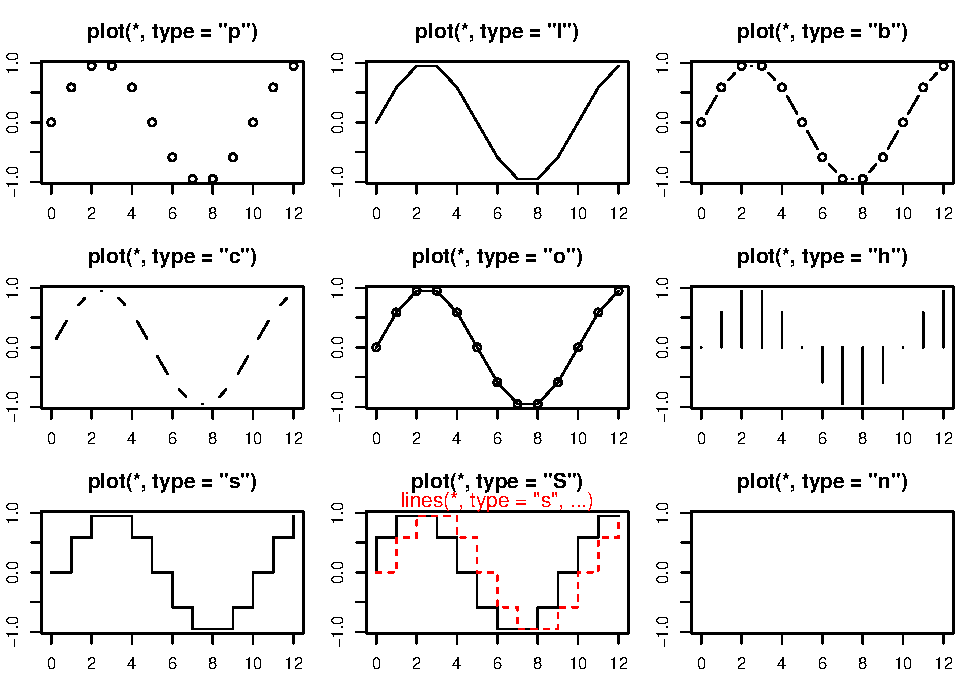
\includegraphics{TudodoR_files/figure-latex/unnamed-chunk-154-1.pdf}

Vamos inserir no gráfico linhas ligando os pontos. Use o argumento *type=``l'' na função \texttt{plot()}:

\begin{Shaded}
\begin{Highlighting}[]
\KeywordTok{plot}\NormalTok{(solo1}\OperatorTok{$}\NormalTok{ds,solo1}\OperatorTok{$}\NormalTok{ptotal, }\DataTypeTok{type =} \StringTok{"l"}\NormalTok{)}
\end{Highlighting}
\end{Shaded}

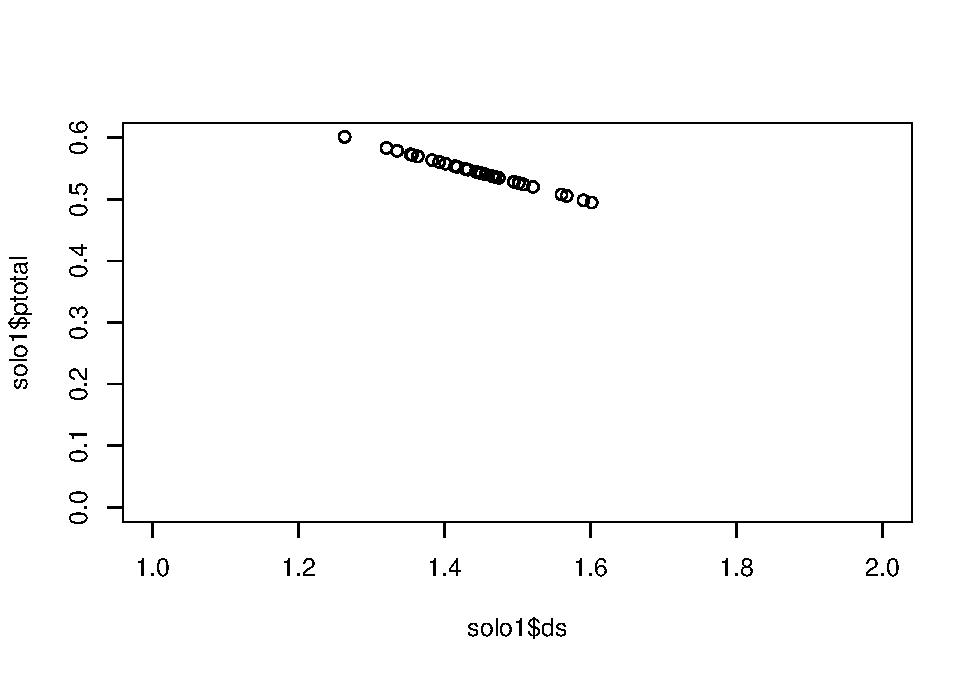
\includegraphics{TudodoR_files/figure-latex/unnamed-chunk-155-1.pdf}

Verifique outras opcões para os gráfico:

\begin{itemize}
\tightlist
\item
  \emph{type = ``p''} especifica o tipo de plotagem
\item
  \emph{``p''}: pontos,
\item
  \emph{``l''}: linhas,
\item
  \emph{``b''}: pontos conectados por linhas,
\item
  \emph{``o''}: id. mas as linhas estão acima dos pontos,
\item
  \emph{``h''}: linhas verticais,
\item
  \emph{``s''}: passos, os dados são representados pelo topo das linhas verticais,
\item
  \emph{``S''}: id. mas os dados são representados pela parte inferior das linhas verticais
\end{itemize}

\begin{Shaded}
\begin{Highlighting}[]
\NormalTok{x <-}\StringTok{ }\DecValTok{0}\OperatorTok{:}\DecValTok{12}
\NormalTok{y <-}\StringTok{ }\KeywordTok{sin}\NormalTok{(pi}\OperatorTok{/}\DecValTok{5} \OperatorTok{*}\StringTok{ }\NormalTok{x)}
\NormalTok{op <-}\StringTok{ }\KeywordTok{par}\NormalTok{(}\DataTypeTok{mfrow =} \KeywordTok{c}\NormalTok{(}\DecValTok{3}\NormalTok{,}\DecValTok{3}\NormalTok{), }\DataTypeTok{mar =} \FloatTok{.1}\OperatorTok{+}\StringTok{ }\KeywordTok{c}\NormalTok{(}\DecValTok{2}\NormalTok{,}\DecValTok{2}\NormalTok{,}\DecValTok{3}\NormalTok{,}\DecValTok{1}\NormalTok{))}
\ControlFlowTok{for}\NormalTok{ (tp }\ControlFlowTok{in} \KeywordTok{c}\NormalTok{(}\StringTok{"p"}\NormalTok{,}\StringTok{"l"}\NormalTok{,}\StringTok{"b"}\NormalTok{,  }\StringTok{"c"}\NormalTok{,}\StringTok{"o"}\NormalTok{,}\StringTok{"h"}\NormalTok{,  }\StringTok{"s"}\NormalTok{,}\StringTok{"S"}\NormalTok{,}\StringTok{"n"}\NormalTok{)) \{}
  \KeywordTok{plot}\NormalTok{(y }\OperatorTok{~}\StringTok{ }\NormalTok{x, }\DataTypeTok{type =}\NormalTok{ tp, }\DataTypeTok{main =} \KeywordTok{paste0}\NormalTok{(}\StringTok{"plot(*, type = }\CharTok{\textbackslash{}"}\StringTok{"}\NormalTok{, tp, }\StringTok{"}\CharTok{\textbackslash{}"}\StringTok{)"}\NormalTok{))}
  \ControlFlowTok{if}\NormalTok{(tp }\OperatorTok{==}\StringTok{ "S"}\NormalTok{) \{}
    \KeywordTok{lines}\NormalTok{(x, y, }\DataTypeTok{type =} \StringTok{"s"}\NormalTok{, }\DataTypeTok{col =} \StringTok{"red"}\NormalTok{, }\DataTypeTok{lty =} \DecValTok{2}\NormalTok{)}
    \KeywordTok{mtext}\NormalTok{(}\StringTok{"lines(*, type = }\CharTok{\textbackslash{}"}\StringTok{s}\CharTok{\textbackslash{}"}\StringTok{, ...)"}\NormalTok{, }\DataTypeTok{col =} \StringTok{"red"}\NormalTok{, }\DataTypeTok{cex =} \FloatTok{0.8}\NormalTok{)}
\NormalTok{  \}}
\NormalTok{\}}
\end{Highlighting}
\end{Shaded}

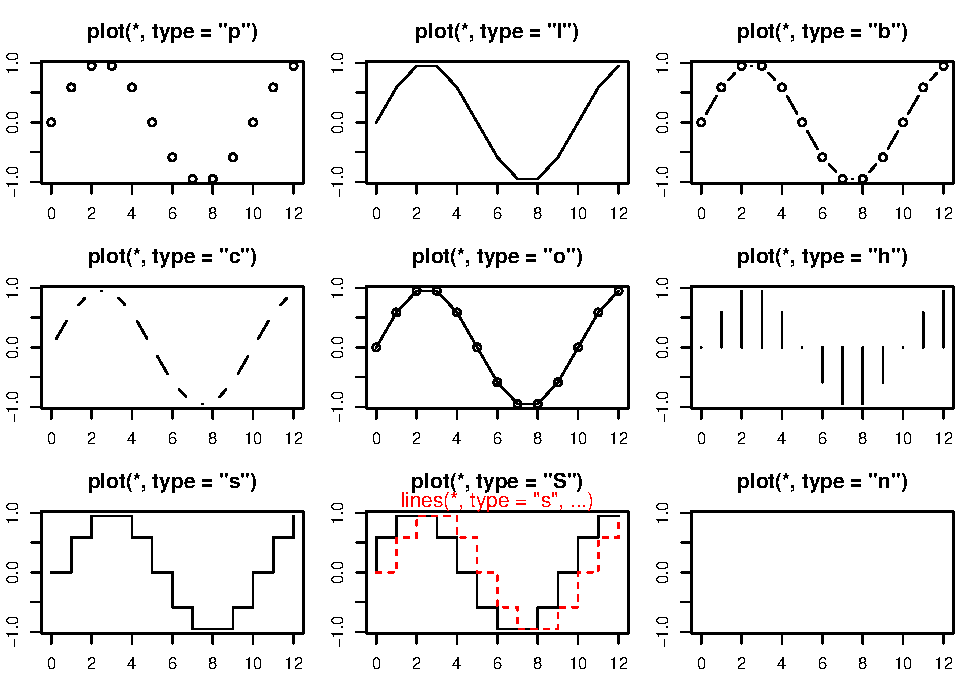
\includegraphics{TudodoR_files/figure-latex/unnamed-chunk-156-1.pdf}

\begin{Shaded}
\begin{Highlighting}[]
\KeywordTok{par}\NormalTok{(op)}
\end{Highlighting}
\end{Shaded}

\hypertarget{mudando-o-padruxe3o-dos-pontos-pch}{%
\subsection{\texorpdfstring{Mudando o padrão dos pontos \texttt{pch=}}{Mudando o padrão dos pontos pch=}}\label{mudando-o-padruxe3o-dos-pontos-pch}}

Pode-se usar diferentes padrões para os pontos usando o argumento \texttt{pch=}. Diferentes tipos de símbolos são associados a diferentes números. Pode-se ainda usar caracteres como o símbolo desejado.
Use a opção \texttt{pch\ =} para especificar símbolos a serem usados ao traçar pontos. Para os símbolos de 21 a 25, especifique a cor da borda \texttt{(col\ =)}:

\begin{Shaded}
\begin{Highlighting}[]
\KeywordTok{plot}\NormalTok{(solo1}\OperatorTok{$}\NormalTok{ds,solo1}\OperatorTok{$}\NormalTok{ptotal, }\DataTypeTok{pch=}\DecValTok{21}\NormalTok{, }\DataTypeTok{ylim =} \KeywordTok{c}\NormalTok{(}\DecValTok{0}\NormalTok{,}\FloatTok{0.6}\NormalTok{), }\DataTypeTok{xlim =} \KeywordTok{c}\NormalTok{(}\DecValTok{1}\NormalTok{,}\DecValTok{2}\NormalTok{))}
\end{Highlighting}
\end{Shaded}

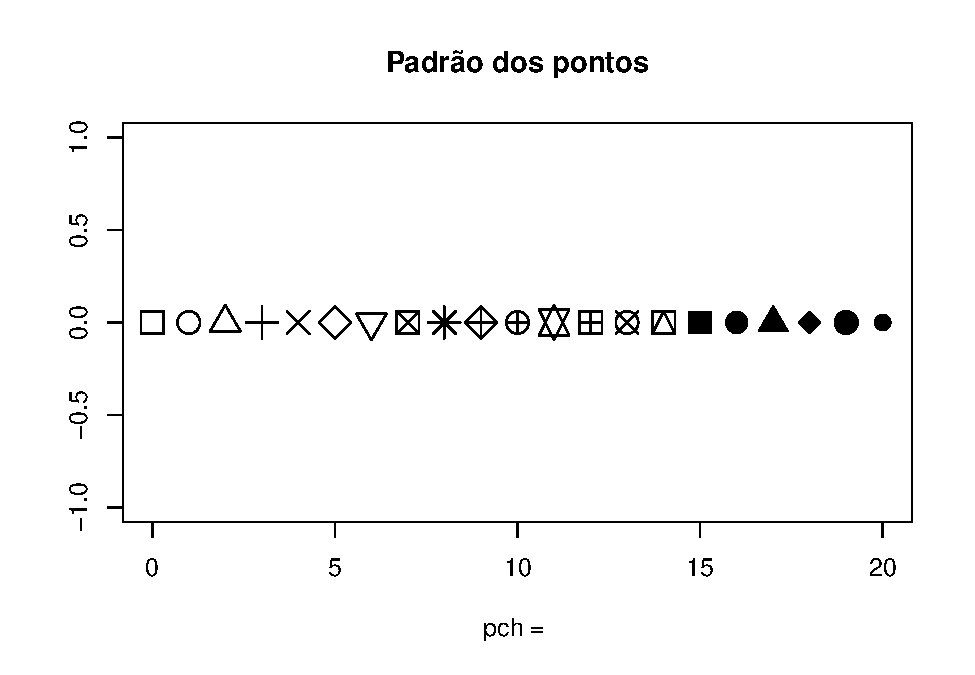
\includegraphics{TudodoR_files/figure-latex/unnamed-chunk-157-1.pdf}

\begin{Shaded}
\begin{Highlighting}[]
\KeywordTok{plot}\NormalTok{(solo2}\OperatorTok{$}\NormalTok{ds,solo2}\OperatorTok{$}\NormalTok{ptotal,}\DataTypeTok{pch=}\DecValTok{2}\NormalTok{, }\DataTypeTok{col=}\StringTok{"blue"}\NormalTok{) }
\end{Highlighting}
\end{Shaded}

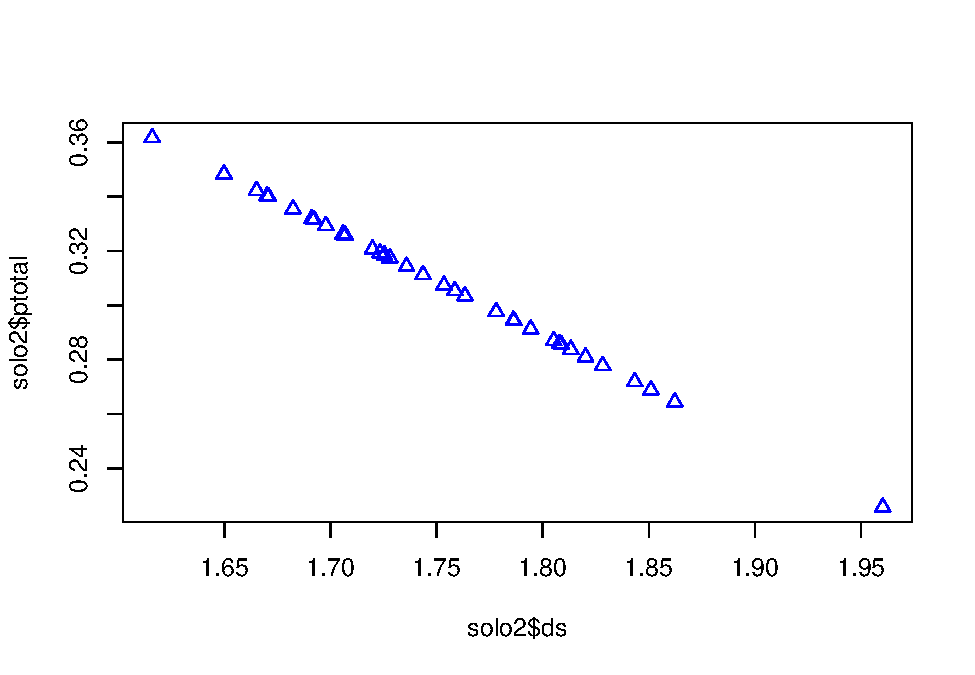
\includegraphics{TudodoR_files/figure-latex/unnamed-chunk-157-2.pdf}

\begin{Shaded}
\begin{Highlighting}[]
\KeywordTok{plot}\NormalTok{(solo3}\OperatorTok{$}\NormalTok{ds,solo3}\OperatorTok{$}\NormalTok{ptotal,}\DataTypeTok{pch=}\StringTok{"%"}\NormalTok{)}
\end{Highlighting}
\end{Shaded}

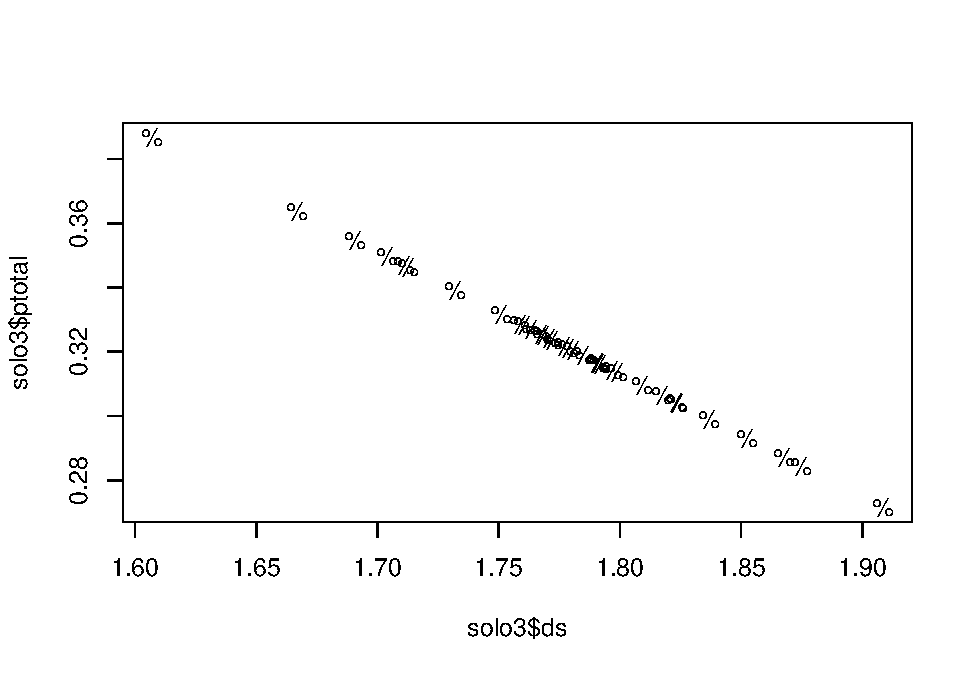
\includegraphics{TudodoR_files/figure-latex/unnamed-chunk-157-3.pdf}

Neste exemplo acima note que foi adicionado o argumento \texttt{ylim} e \texttt{xlim} eles limitam os valores mínimos e máximos:

\begin{Shaded}
\begin{Highlighting}[]
\NormalTok{xlim=}\KeywordTok{c}\NormalTok{(xmin, xmax) ylim=}\KeywordTok{c}\NormalTok{(ymin, ymax)}\ErrorTok{)}
\end{Highlighting}
\end{Shaded}

Veja um exemplo do padrão dos pontos:

\begin{Shaded}
\begin{Highlighting}[]
\KeywordTok{plot}\NormalTok{ (}\DecValTok{0}\OperatorTok{:}\DecValTok{20}\NormalTok{,                         }\CommentTok{#coord. eixo X}
      \KeywordTok{rep}\NormalTok{ (}\DecValTok{0}\NormalTok{,}\DecValTok{21}\NormalTok{),                   }\CommentTok{#coord. eixo y}
      \DataTypeTok{pch =} \DecValTok{0}\OperatorTok{:}\DecValTok{20}\NormalTok{,                   }\CommentTok{#padrão dos pontos variando}
      \DataTypeTok{cex =} \DecValTok{2}\NormalTok{,                      }\CommentTok{#tamanho dos pontos}
      \DataTypeTok{main =} \StringTok{"Padrão dos pontos"}\NormalTok{, }\CommentTok{#Titulo (note o \textbackslash{}n)}
      \DataTypeTok{xlab =} \StringTok{"pch = "}\NormalTok{,              }\CommentTok{#texto do eixo de x}
      \DataTypeTok{ylab =} \StringTok{""}\NormalTok{)                    }\CommentTok{#texto do eixo de y}
\end{Highlighting}
\end{Shaded}

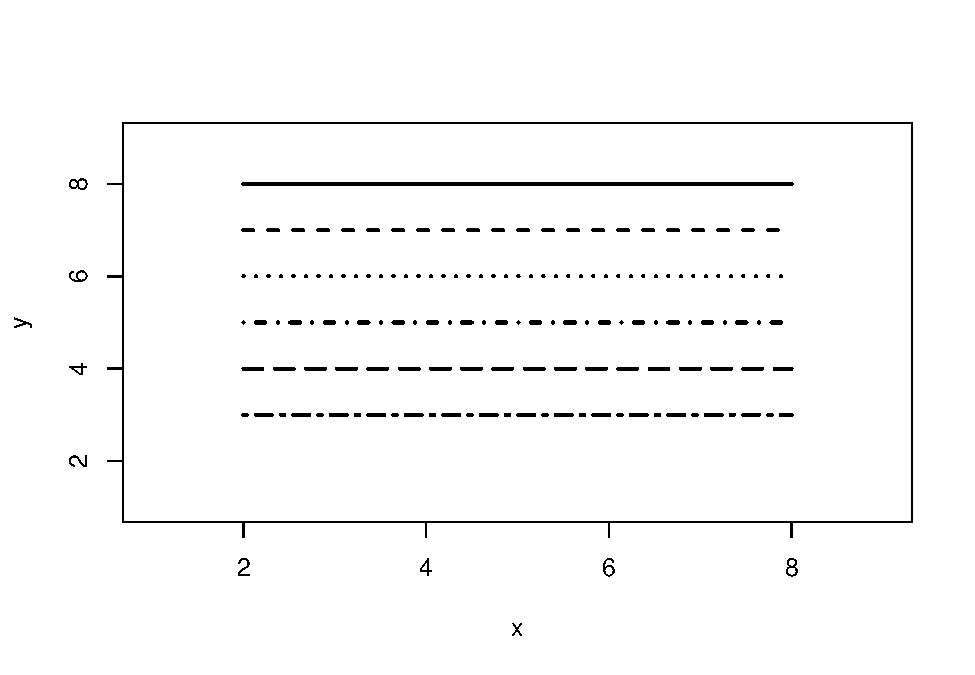
\includegraphics{TudodoR_files/figure-latex/unnamed-chunk-159-1.pdf}

\hypertarget{mudando-as-linhas-lwd-e-lty}{%
\subsection{\texorpdfstring{Mudando as linhas (\texttt{lwd\ e\ lty})}{Mudando as linhas (lwd e lty)}}\label{mudando-as-linhas-lwd-e-lty}}

Você pode alterar linhas usando as seguintes opções. Isso é particularmente útil para linhas de referência, eixos e linhas de ajuste. A largura das linhas pode ser mudada com o argumento \texttt{lwd=}, enquanto os estilos das linhas podem ser modificados com o argumento \texttt{lty=}:

\begin{Shaded}
\begin{Highlighting}[]
\KeywordTok{plot}\NormalTok{(solo3}\OperatorTok{$}\NormalTok{ds,solo3}\OperatorTok{$}\NormalTok{ptotal, }\DataTypeTok{lwd=}\DecValTok{2}\NormalTok{) }\CommentTok{# linha grossa}
\end{Highlighting}
\end{Shaded}

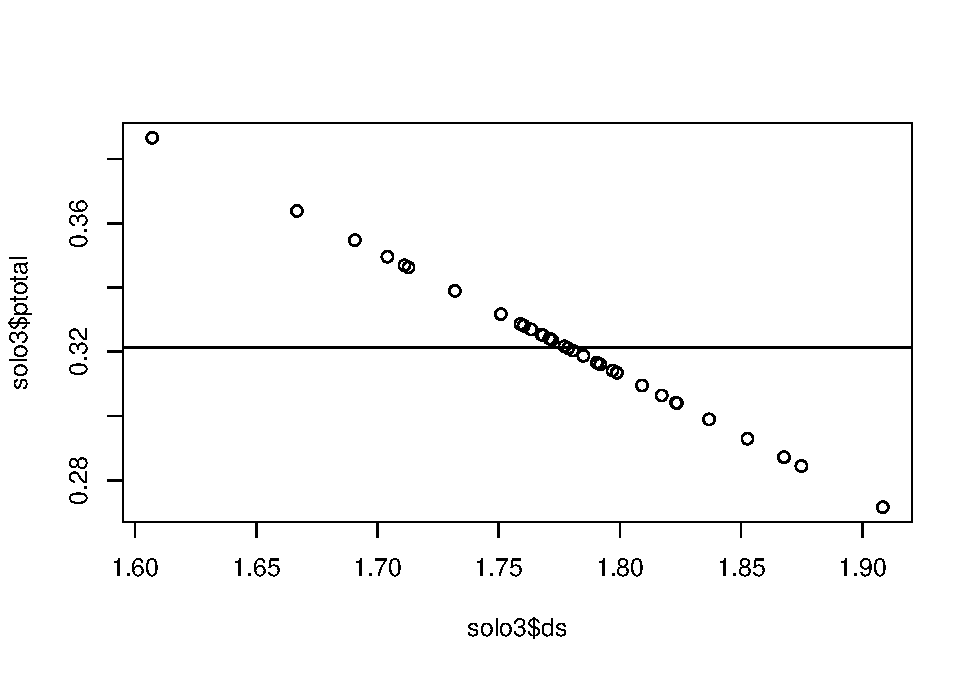
\includegraphics{TudodoR_files/figure-latex/unnamed-chunk-160-1.pdf}

\begin{Shaded}
\begin{Highlighting}[]
\KeywordTok{plot}\NormalTok{(solo2}\OperatorTok{$}\NormalTok{ds,solo2}\OperatorTok{$}\NormalTok{ptotal, }\DataTypeTok{lty=}\DecValTok{2}\NormalTok{) }\CommentTok{#linha interrompida}
\end{Highlighting}
\end{Shaded}

\includegraphics{TudodoR_files/figure-latex/unnamed-chunk-160-2.pdf}

\begin{Shaded}
\begin{Highlighting}[]
\NormalTok{x <-}\StringTok{ }\DecValTok{1}\OperatorTok{:}\DecValTok{9}
\NormalTok{y <-}\StringTok{ }\DecValTok{1}\OperatorTok{:}\DecValTok{9}
  \KeywordTok{plot}\NormalTok{(x, y, }\DataTypeTok{type =} \StringTok{"n"}\NormalTok{)}
    \KeywordTok{lines}\NormalTok{(}\KeywordTok{c}\NormalTok{(}\DecValTok{2}\NormalTok{, }\DecValTok{8}\NormalTok{), }\KeywordTok{c}\NormalTok{(}\DecValTok{8}\NormalTok{, }\DecValTok{8}\NormalTok{), }\DataTypeTok{lwd =} \DecValTok{2}\NormalTok{)}
    \KeywordTok{lines}\NormalTok{(}\KeywordTok{c}\NormalTok{(}\DecValTok{2}\NormalTok{, }\DecValTok{8}\NormalTok{), }\KeywordTok{c}\NormalTok{(}\DecValTok{7}\NormalTok{, }\DecValTok{7}\NormalTok{), }\DataTypeTok{lty =} \DecValTok{2}\NormalTok{, }\DataTypeTok{lwd =} \DecValTok{2}\NormalTok{)}
    \KeywordTok{lines}\NormalTok{(}\KeywordTok{c}\NormalTok{(}\DecValTok{2}\NormalTok{, }\DecValTok{8}\NormalTok{), }\KeywordTok{c}\NormalTok{(}\DecValTok{6}\NormalTok{, }\DecValTok{6}\NormalTok{), }\DataTypeTok{lty =} \DecValTok{3}\NormalTok{, }\DataTypeTok{lwd =} \DecValTok{2}\NormalTok{)}
    \KeywordTok{lines}\NormalTok{(}\KeywordTok{c}\NormalTok{(}\DecValTok{2}\NormalTok{, }\DecValTok{8}\NormalTok{), }\KeywordTok{c}\NormalTok{(}\DecValTok{5}\NormalTok{, }\DecValTok{5}\NormalTok{), }\DataTypeTok{lty =} \DecValTok{4}\NormalTok{, }\DataTypeTok{lwd =} \DecValTok{2}\NormalTok{)}
    \KeywordTok{lines}\NormalTok{(}\KeywordTok{c}\NormalTok{(}\DecValTok{2}\NormalTok{, }\DecValTok{8}\NormalTok{), }\KeywordTok{c}\NormalTok{(}\DecValTok{4}\NormalTok{, }\DecValTok{4}\NormalTok{), }\DataTypeTok{lty =} \DecValTok{5}\NormalTok{, }\DataTypeTok{lwd =} \DecValTok{2}\NormalTok{)}
    \KeywordTok{lines}\NormalTok{(}\KeywordTok{c}\NormalTok{(}\DecValTok{2}\NormalTok{, }\DecValTok{8}\NormalTok{), }\KeywordTok{c}\NormalTok{(}\DecValTok{3}\NormalTok{, }\DecValTok{3}\NormalTok{), }\DataTypeTok{lty =} \DecValTok{6}\NormalTok{, }\DataTypeTok{lwd =} \DecValTok{2}\NormalTok{)}
\end{Highlighting}
\end{Shaded}

\includegraphics{TudodoR_files/figure-latex/unnamed-chunk-161-1.pdf}

\hypertarget{adicionando-linhas-a-um-grafico-de-pontos}{%
\subsection{Adicionando linhas a um grafico de pontos}\label{adicionando-linhas-a-um-grafico-de-pontos}}

A função utilizada para inserir linhas é \texttt{abline()}.
Vamos usar a função \texttt{abline} para inserir uma linha que mostra a média dos dados do eixo Y.
o h é de linha horizontal. Fará uma linha na horizontal que passa pela média de y.

\begin{Shaded}
\begin{Highlighting}[]
\KeywordTok{plot}\NormalTok{(solo3}\OperatorTok{$}\NormalTok{ds,solo3}\OperatorTok{$}\NormalTok{ptotal, }\KeywordTok{abline}\NormalTok{(}\DataTypeTok{h=}\KeywordTok{mean}\NormalTok{(solo3}\OperatorTok{$}\NormalTok{ptotal))) }
\end{Highlighting}
\end{Shaded}

\includegraphics{TudodoR_files/figure-latex/unnamed-chunk-162-1.pdf}

Para passar uma linha que passa pela média de x:

\begin{Shaded}
\begin{Highlighting}[]
\KeywordTok{plot}\NormalTok{(solo3}\OperatorTok{$}\NormalTok{ds,solo3}\OperatorTok{$}\NormalTok{ptotal)}
\end{Highlighting}
\end{Shaded}

\includegraphics{TudodoR_files/figure-latex/unnamed-chunk-163-1.pdf}

\begin{Shaded}
\begin{Highlighting}[]
\KeywordTok{plot}\NormalTok{(solo3}\OperatorTok{$}\NormalTok{ds,solo3}\OperatorTok{$}\NormalTok{ptotal, }\KeywordTok{abline}\NormalTok{(}\DataTypeTok{v=}\KeywordTok{mean}\NormalTok{(solo3}\OperatorTok{$}\NormalTok{ds))) }\CommentTok{## o v é de vertical}
\end{Highlighting}
\end{Shaded}

\includegraphics{TudodoR_files/figure-latex/unnamed-chunk-164-1.pdf}

Também é possível inserir as duas linhas ao mesmo tempo:

\begin{Shaded}
\begin{Highlighting}[]
\KeywordTok{plot}\NormalTok{(solo3}\OperatorTok{$}\NormalTok{ds,solo3}\OperatorTok{$}\NormalTok{ptotal, }\KeywordTok{abline}\NormalTok{(}\DataTypeTok{h=}\KeywordTok{mean}\NormalTok{(solo3}\OperatorTok{$}\NormalTok{ptotal), }\DataTypeTok{v=}\KeywordTok{mean}\NormalTok{(solo3}\OperatorTok{$}\NormalTok{ds),}\DataTypeTok{col=}\StringTok{"red"}\NormalTok{))}
\end{Highlighting}
\end{Shaded}

\includegraphics{TudodoR_files/figure-latex/unnamed-chunk-165-1.pdf}

Com cores diferentes:

\begin{Shaded}
\begin{Highlighting}[]
\KeywordTok{plot}\NormalTok{(solo3}\OperatorTok{$}\NormalTok{ds,solo3}\OperatorTok{$}\NormalTok{ptotal, }\KeywordTok{abline}\NormalTok{(}\DataTypeTok{h=}\KeywordTok{mean}\NormalTok{(solo3}\OperatorTok{$}\NormalTok{ptotal), }\DataTypeTok{v=}\KeywordTok{mean}\NormalTok{(solo3}\OperatorTok{$}\NormalTok{ds),}\DataTypeTok{col=}\KeywordTok{c}\NormalTok{(}\DecValTok{2}\NormalTok{,}\DecValTok{4}\NormalTok{)))}
\end{Highlighting}
\end{Shaded}

\includegraphics{TudodoR_files/figure-latex/unnamed-chunk-166-1.pdf}

\hypertarget{definindo-o-intervalo-dos-eixos}{%
\subsection{Definindo o intervalo dos eixos}\label{definindo-o-intervalo-dos-eixos}}

Se você quiser preencher um mesmo gráfico com linhas e pontos que possuem diferentes amplitudes como nosso exemplo do solos, deve usar o argumento \texttt{type=n}. Com este argumento um gráfico em branco é criado.

\begin{Shaded}
\begin{Highlighting}[]
\KeywordTok{plot}\NormalTok{(}\KeywordTok{c}\NormalTok{(}\FloatTok{1.55}\NormalTok{,}\DecValTok{2}\NormalTok{),}\KeywordTok{c}\NormalTok{(}\DecValTok{0}\NormalTok{,}\FloatTok{0.6}\NormalTok{),}\DataTypeTok{type=}\StringTok{'n'}\NormalTok{)}
\KeywordTok{points}\NormalTok{(solo3}\OperatorTok{$}\NormalTok{ds,solo3}\OperatorTok{$}\NormalTok{ptotal, }\DataTypeTok{pch=}\DecValTok{2}\NormalTok{)}
\KeywordTok{points}\NormalTok{(solo2}\OperatorTok{$}\NormalTok{ds,solo2}\OperatorTok{$}\NormalTok{ptotal)}
\end{Highlighting}
\end{Shaded}

\includegraphics{TudodoR_files/figure-latex/unnamed-chunk-167-1.pdf}

\hypertarget{personalizando-os-gruxe1ficos}{%
\subsection{Personalizando os gráficos}\label{personalizando-os-gruxe1ficos}}

Alguns parâmetros podem ser usados no intuito de personalizar um gráfico no R.

Exemplo:

\begin{Shaded}
\begin{Highlighting}[]
\KeywordTok{plot}\NormalTok{(solo1}\OperatorTok{$}\NormalTok{ptotal,solo1}\OperatorTok{$}\NormalTok{ds)}
\end{Highlighting}
\end{Shaded}

\includegraphics{TudodoR_files/figure-latex/unnamed-chunk-168-1.pdf}

\begin{Shaded}
\begin{Highlighting}[]
\KeywordTok{plot}\NormalTok{(solo1}\OperatorTok{$}\NormalTok{ptotal,solo1}\OperatorTok{$}\NormalTok{ds,          }\CommentTok{#plota ds e ptotal}
\DataTypeTok{xlab=}\StringTok{"Macroporosdiade (%)"}\NormalTok{,          }\CommentTok{#nomeia o eixo x}
\DataTypeTok{ylab=}\KeywordTok{expression}\NormalTok{(Ds}\OperatorTok{~}\NormalTok{(mg}\OperatorTok{~}\NormalTok{Kg}\OperatorTok{^}\NormalTok{\{}\OperatorTok{-}\DecValTok{1}\NormalTok{\})),    }\CommentTok{#nomeia o eixo y}
\DataTypeTok{main=}\StringTok{"Como personalizar um gráfico"}\NormalTok{, }\CommentTok{#referente ao título}
\DataTypeTok{xlim=}\KeywordTok{c}\NormalTok{(}\FloatTok{0.48}\NormalTok{,}\FloatTok{0.64}\NormalTok{),                   }\CommentTok{#limites do eixo x}
\DataTypeTok{ylim=}\KeywordTok{c}\NormalTok{(}\DecValTok{0}\NormalTok{,}\DecValTok{2}\NormalTok{), }\DataTypeTok{col=}\StringTok{"red"}\NormalTok{,              }\CommentTok{#limites do eixo y}
\DataTypeTok{pch=}\DecValTok{22}\NormalTok{,                              }\CommentTok{#padrão dos pontos}
\DataTypeTok{bg=}\StringTok{"yellow"}\NormalTok{,                         }\CommentTok{#cor de preenchimento}
\DataTypeTok{tcl=}\FloatTok{0.4}\NormalTok{,                             }\CommentTok{#tamanho dos traços dos eixos}
\DataTypeTok{las=}\DecValTok{1}\NormalTok{,                               }\CommentTok{#orientação do texto em y}
\DataTypeTok{cex=}\FloatTok{1.5}\NormalTok{,                             }\CommentTok{#tamanho do objeto do ponto}
\DataTypeTok{bty=}\StringTok{"l"}\NormalTok{,                             }\CommentTok{#altera as bordas}
\KeywordTok{abline}\NormalTok{(}\KeywordTok{lm}\NormalTok{(solo1}\OperatorTok{$}\NormalTok{ds}\OperatorTok{~}\NormalTok{solo1}\OperatorTok{$}\NormalTok{ptotal)))   }\CommentTok{#regressao dos pontos}
\end{Highlighting}
\end{Shaded}

\includegraphics{TudodoR_files/figure-latex/unnamed-chunk-168-2.pdf}

Veja o \texttt{demo(plotmath)} para saber mais sobre anotações em gráficos.

\hypertarget{histogramas}{%
\section{Histogramas}\label{histogramas}}

A função \texttt{hist()} produz um histograma dos dados informados em seu argumento enquanto a função \texttt{barplot()} produz um gráfico de barras:

\begin{Shaded}
\begin{Highlighting}[]
\KeywordTok{hist}\NormalTok{(solo1}\OperatorTok{$}\NormalTok{ds)}
\KeywordTok{rug}\NormalTok{(solo1}\OperatorTok{$}\NormalTok{ds)}
\end{Highlighting}
\end{Shaded}

\includegraphics{TudodoR_files/figure-latex/unnamed-chunk-169-1.pdf}

\hypertarget{personalizando-gruxe1ficos}{%
\subsection{Personalizando gráficos}\label{personalizando-gruxe1ficos}}

Os histogramas criados no R seguem um certo padrão (conhecido como parâmetros
default) que podem ser alterados de acordo com a preferência do usuário. Você pode obter informações detalhadas desses parâmetros se usar os recursos de ajuda do R:

\begin{Shaded}
\begin{Highlighting}[]
\KeywordTok{hist}\NormalTok{(solo1}\OperatorTok{$}\NormalTok{ds, }\CommentTok{#histograma de ds}
     \DataTypeTok{main=}\StringTok{"Histograma Personalizado}\CharTok{\textbackslash{}n}\StringTok{densidade do solo"}\NormalTok{,}\CommentTok{#título}
     \DataTypeTok{xlab=}\KeywordTok{expression}\NormalTok{(Ds}\OperatorTok{~}\NormalTok{(mg}\OperatorTok{~}\NormalTok{Kg}\OperatorTok{^}\NormalTok{\{}\OperatorTok{-}\DecValTok{1}\NormalTok{\})), }\CommentTok{#texto do eixo das abscissas}
     \DataTypeTok{ylab=}\StringTok{"Probabilidades"}\NormalTok{, }\CommentTok{#texto do eixo das ordenadas}
     \DataTypeTok{xlim=}\KeywordTok{c}\NormalTok{(}\DecValTok{1}\NormalTok{,}\DecValTok{2}\NormalTok{), }\CommentTok{#limites do eixo de x}
     \DataTypeTok{ylim=}\KeywordTok{c}\NormalTok{(}\DecValTok{0}\NormalTok{,}\DecValTok{10}\NormalTok{), }\CommentTok{#limites do eixo y}
     \DataTypeTok{col=}\StringTok{"lightblue"}\NormalTok{, }\CommentTok{#cor das colunas}
     \DataTypeTok{border=}\StringTok{"white"}\NormalTok{, }\CommentTok{#cor das bordas das colunas}
     \DataTypeTok{adj=}\DecValTok{0}\NormalTok{, }\CommentTok{#alinhamento dos textos 0, 0.5 e 1}
     \DataTypeTok{col.axis=}\StringTok{"red"}\NormalTok{) }\CommentTok{#cor do texto nos eixos}
\end{Highlighting}
\end{Shaded}

\includegraphics{TudodoR_files/figure-latex/unnamed-chunk-170-1.pdf}

\hypertarget{gruxe1ficos-de-barras}{%
\section{Gráficos de Barras}\label{gruxe1ficos-de-barras}}

Assemelha-se ao histograma, porém nesse caso os dados referem-se a categoria ou aos tratamentos:

\begin{Shaded}
\begin{Highlighting}[]
\KeywordTok{barplot}\NormalTok{(solo}\OperatorTok{$}\NormalTok{ptotal,}\DataTypeTok{names.arg=}\NormalTok{solo}\OperatorTok{$}\NormalTok{z, }\DataTypeTok{horiz =}\NormalTok{ T)}
\end{Highlighting}
\end{Shaded}

\includegraphics{TudodoR_files/figure-latex/unnamed-chunk-171-1.pdf}

\hypertarget{boxplots}{%
\section{Boxplots}\label{boxplots}}

Dados de um experimento visando controle de pulgão (\emph{Aphis gossypii Glover}) em cultura de pepino, instalado em \emph{delineamento inteiramente casualizado} com 6 repetições. A resposta observada foi o número de pulgões após a aplicação de produtos indicados para seu controle.

\begin{Shaded}
\begin{Highlighting}[]
\NormalTok{dados <-}\StringTok{ }\KeywordTok{read.table}\NormalTok{(}\StringTok{"https://www.dropbox.com/s/jjyo8dhyy0qt3ft/BanzattoQd3.2.1.txt?dl=1"}\NormalTok{)}
\KeywordTok{str}\NormalTok{(dados)}
\end{Highlighting}
\end{Shaded}

\begin{verbatim}
## 'data.frame':    30 obs. of  3 variables:
##  $ trat   : Factor w/ 5 levels "Azinfos etilico",..: 5 1 3 4 2 5 1 3 4 2 ...
##  $ rept   : int  1 1 1 1 1 2 2 2 2 2 ...
##  $ pulgoes: int  2370 1282 562 173 193 1687 1527 321 127 71 ...
\end{verbatim}

\emph{trat}
Fator de níveis nominais. Tratamento aplicado para controle do pulgão.

\emph{rept}
Número inteiro que identifica as repetições de cada tratamento.

\emph{pulgões}
Número de pulgões coletados 36 horas após a pulverização dos tratamentos.

Boxplots podem ser criados para variáveis individuais ou para variáveis por grupo. O formato é \texttt{boxplot} \texttt{(\ x\ ,\ data\ =)} , em que \texttt{x} é uma fórmula e \texttt{data\ =} denota o quadro de dados que fornece os dados.

Um exemplo de uma fórmula é \texttt{y\ \textasciitilde{}\ group} onde um boxplot separado para a variável numérica é gerado para cada valor de group:

\begin{Shaded}
\begin{Highlighting}[]
\KeywordTok{x11}\NormalTok{()}
\KeywordTok{boxplot}\NormalTok{(pulgoes}\OperatorTok{~}\NormalTok{trat,              }\CommentTok{#formula do boxplot}
        \DataTypeTok{data =}\NormalTok{ dados,              }\CommentTok{#conjunto de dados}
        \DataTypeTok{main=}\StringTok{"boxplot"}\NormalTok{,            }\CommentTok{#título}
        \DataTypeTok{xlab=}\StringTok{"Controle do pulgão"}\NormalTok{, }\CommentTok{#texto do eixo x }
        \DataTypeTok{ylab=}\StringTok{"Numero de plugões",  #texto do eixo y}
\StringTok{        col=3)                     #cor verde  }
\end{Highlighting}
\end{Shaded}

\includegraphics{TudodoR_files/figure-latex/unnamed-chunk-173-1.pdf}

Adicione \texttt{horizontal\ =\ TRUE} para inverter a orientação do eixo:

\begin{Shaded}
\begin{Highlighting}[]
\KeywordTok{boxplot}\NormalTok{(pulgoes}\OperatorTok{~}\NormalTok{trat,              }\CommentTok{#formula do boxplot}
        \DataTypeTok{data =}\NormalTok{ dados,              }\CommentTok{#conjunto de dados}
        \DataTypeTok{main=}\StringTok{"boxplot"}\NormalTok{,            }\CommentTok{#t?tulo}
        \DataTypeTok{xlab=}\StringTok{"Controle do pulgão"}\NormalTok{, }\CommentTok{#texto do eixo x }
        \DataTypeTok{ylab=}\StringTok{"Numero de plugões",  #texto do eixo y}
\StringTok{        col=3, horizontal = T,     #cor verde  }
\StringTok{        notch=T)                   #teste para mediana}
\end{Highlighting}
\end{Shaded}

\begin{verbatim}
## Warning in bxp(list(stats = structure(c(825, 871, 972.5, 1282, 1527, 44, : some
## notches went outside hinges ('box'): maybe set notch=FALSE
\end{verbatim}

\includegraphics{TudodoR_files/figure-latex/unnamed-chunk-174-1.pdf}

\hypertarget{boxplot-com-fatorial}{%
\subsection{Boxplot com fatorial}\label{boxplot-com-fatorial}}

Boxplot com 2 fatores, com caixas coloridas para facilitar a interpretação.

\textbf{Efeito de Recipientes para duas Espécies de Eucalipto}

Experimento em esquema fatorial 3x2 para estudar o efeito de 3 tipos de recipientes para a produção de mudas de duas espécies de Eucalipto. O experimento foi instalado em delineamento inteiramente casualizado.

\emph{recipie}
São os níveis de recipiente estudados:
- SPP - saco plástico pequeno;
- SPG - saco plástico grande; e
- Lam - laminado.

\emph{especie}
São as espécies de Eucalipto: \emph{Eucalyptus citriodora} e \emph{Eucalyptus grandis}

\emph{rept}
Identifica as repetições de cada combinação dos fatores recipiente e espécie.

\emph{alt}
Altura das mudas aos 80 dias de idade (cm).

Baixar dados via web:

\begin{Shaded}
\begin{Highlighting}[]
\NormalTok{fat <-}\StringTok{ }\KeywordTok{read.table}\NormalTok{(}\StringTok{"https://www.dropbox.com/s/sahc5n80rlkcfx4/BanzattoQd5.2.4.txt?dl=1"}\NormalTok{)}
\KeywordTok{str}\NormalTok{(fat)}
\end{Highlighting}
\end{Shaded}

\begin{verbatim}
## 'data.frame':    24 obs. of  4 variables:
##  $ recipie: Factor w/ 3 levels "Lam","SPG","SPP": 3 3 2 2 1 1 3 3 2 2 ...
##  $ especie: Factor w/ 2 levels "E. citriodora",..: 1 2 1 2 1 2 1 2 1 2 ...
##  $ rept   : int  1 1 1 1 1 1 2 2 2 2 ...
##  $ alt    : num  26.2 24.8 25.7 19.6 22.8 19.8 26 24.6 26.3 21.1 ...
\end{verbatim}

Gerar o gráfico boxpolt com o comando abaixo:

\begin{Shaded}
\begin{Highlighting}[]
\KeywordTok{boxplot}\NormalTok{(fat}\OperatorTok{$}\NormalTok{alt}\OperatorTok{~}\NormalTok{fat}\OperatorTok{$}\NormalTok{recipie}\OperatorTok{*}\NormalTok{especie, }\DataTypeTok{data=}\NormalTok{fat, }\DataTypeTok{notch=}\NormalTok{F, }
        \DataTypeTok{col=}\NormalTok{(}\KeywordTok{c}\NormalTok{(}\StringTok{"gold"}\NormalTok{,}\StringTok{"darkgreen"}\NormalTok{,}\StringTok{"brown"}\NormalTok{)),}
        \DataTypeTok{main=}\StringTok{"Fatorial"}\NormalTok{, }\DataTypeTok{xlab=}\StringTok{"Recipiente e Espécies"}\NormalTok{,}
        \DataTypeTok{ylab=}\StringTok{"Altura de plantas (cm)"}\NormalTok{)}
\end{Highlighting}
\end{Shaded}

\includegraphics{TudodoR_files/figure-latex/unnamed-chunk-176-1.pdf}

\hypertarget{cores}{%
\section{Cores}\label{cores}}

Gráficos em preto e branco são bons na maioria dos casos, mas cores podem ser mudadas usando \texttt{col="red"} (escrevendo o nome da cor) ou \texttt{col=2} (usando números).
O comando abaixo mostra os números que especificam algumas cores:

\begin{Shaded}
\begin{Highlighting}[]
\KeywordTok{pie}\NormalTok{(}\KeywordTok{rep}\NormalTok{(}\DecValTok{1}\NormalTok{,}\DecValTok{30}\NormalTok{),}\DataTypeTok{col=}\KeywordTok{rainbow}\NormalTok{(}\DecValTok{30}\NormalTok{))}
\end{Highlighting}
\end{Shaded}

\includegraphics{TudodoR_files/figure-latex/unnamed-chunk-177-1.pdf}

Veja sua tabela de cores executando o script: \href{https://www.dropbox.com/s/e9a27z97buqjovz/paletadecores.R?dl=1}{paletedecores.R}.

Podemos também criar cores personalizadas usando a função do \texttt{rgb()}, que recebe como argumentos as quantidades de vermelho \emph{(red)}, verde \emph{(green)} e azul \emph{(blue)} e, opcionalmente, o grau de opacidade (alpha). Os valores devem ser números reais entre 0 e 1.

Exemplos:

\begin{Shaded}
\begin{Highlighting}[]
\NormalTok{goiaba <-}\StringTok{ }\KeywordTok{rgb}\NormalTok{(}\FloatTok{0.94}\NormalTok{, }\FloatTok{0.41}\NormalTok{, }\FloatTok{0.40}\NormalTok{)}
\NormalTok{goiaba.semitrans <-}\StringTok{ }\KeywordTok{rgb}\NormalTok{(}\FloatTok{0.94}\NormalTok{, }\FloatTok{0.41}\NormalTok{, }\FloatTok{0.40}\NormalTok{, }\DataTypeTok{alpha =} \FloatTok{0.5}\NormalTok{)}
\NormalTok{vitamina <-}\StringTok{ }\KeywordTok{rgb}\NormalTok{(}\DataTypeTok{red =} \KeywordTok{c}\NormalTok{(}\FloatTok{0.87}\NormalTok{, }\FloatTok{0.70}\NormalTok{), }\DataTypeTok{green =} \KeywordTok{c}\NormalTok{(}\FloatTok{0.83}\NormalTok{, }\FloatTok{0.77}\NormalTok{),}
\DataTypeTok{blue =} \KeywordTok{c}\NormalTok{(}\FloatTok{0.71}\NormalTok{, }\FloatTok{0.30}\NormalTok{), }\DataTypeTok{names =} \KeywordTok{c}\NormalTok{(}\StringTok{"leite"}\NormalTok{, }\StringTok{"abacate"}\NormalTok{))}
\end{Highlighting}
\end{Shaded}

\hypertarget{interagindo-com-a-janela-gruxe1fica}{%
\section{Interagindo com a Janela gráfica}\label{interagindo-com-a-janela-gruxe1fica}}

Poderemos com o mouse marcar a ponte desejada usando a função \texttt{identify\ ()}:

\begin{Shaded}
\begin{Highlighting}[]
\KeywordTok{plot}\NormalTok{(solo1}\OperatorTok{$}\NormalTok{ds}\OperatorTok{~}\NormalTok{solo1}\OperatorTok{$}\NormalTok{ptotal)}
\KeywordTok{identify}\NormalTok{(solo1}\OperatorTok{$}\NormalTok{ds,}\DataTypeTok{n=}\DecValTok{1}\NormalTok{)}
\end{Highlighting}
\end{Shaded}

\includegraphics{TudodoR_files/figure-latex/unnamed-chunk-179-1.pdf}

\begin{verbatim}
## integer(0)
\end{verbatim}

\hypertarget{texto-e-tamanho-do-suxedmbolo}{%
\section{Texto e tamanho do símbolo}\label{texto-e-tamanho-do-suxedmbolo}}

As seguintes opções podem ser usadas para controlar o tamanho do texto e do símbolo em gráficos.

\texttt{cex} número que indica o valor pelo qual o texto e os símbolos de plotagem devem ser dimensionados em relação ao padrão.
\emph{1 = padrão, 1,5 é 50\% maior, 0,5 é 50\% menor, etc.}

\hypertarget{visualizar-vuxe1rios-gruxe1ficos}{%
\section{Visualizar vários gráficos}\label{visualizar-vuxe1rios-gruxe1ficos}}

\begin{Shaded}
\begin{Highlighting}[]
\KeywordTok{x11}\NormalTok{()}
\KeywordTok{boxplot}\NormalTok{(pulgoes}\OperatorTok{~}\NormalTok{trat,              }\CommentTok{#formula do boxplot}
        \DataTypeTok{data =}\NormalTok{ dados,              }\CommentTok{#conjunto de dados}
        \DataTypeTok{main=}\StringTok{"boxplot"}\NormalTok{,            }\CommentTok{#título}
        \DataTypeTok{xlab=}\StringTok{"Controle do pulgão"}\NormalTok{, }\CommentTok{#texto do eixo x }
        \DataTypeTok{ylab=}\StringTok{"Numero de plugões",  #texto do eixo y}
\StringTok{        col=3,                     #cor verde  }
\StringTok{        notch=F)                   #teste para mediana}
\end{Highlighting}
\end{Shaded}

\includegraphics{TudodoR_files/figure-latex/unnamed-chunk-181-1.pdf}

\hypertarget{varios-gruxe1ficos-na-mesma-janela-gruxe1fica}{%
\subsection{Varios gráficos na mesma janela gráfica}\label{varios-gruxe1ficos-na-mesma-janela-gruxe1fica}}

Você pode dar instruções para o programa mostrar diversos gráficos pequenos em uma mesma janela ao invés de um apenas. Para isto use a função \texttt{par()}.

\textbf{Exemplo 1}

\begin{Shaded}
\begin{Highlighting}[]
\KeywordTok{par}\NormalTok{(}\DataTypeTok{mfrow =} \KeywordTok{c}\NormalTok{(}\DecValTok{2}\NormalTok{,}\DecValTok{2}\NormalTok{)) }\CommentTok{#2 linhas e 2 colunas}
\KeywordTok{plot}\NormalTok{(solo1}\OperatorTok{$}\NormalTok{ptotal,solo1}\OperatorTok{$}\NormalTok{ds)}
\KeywordTok{boxplot}\NormalTok{(solo1}\OperatorTok{$}\NormalTok{ds,solo2}\OperatorTok{$}\NormalTok{ds, solo3}\OperatorTok{$}\NormalTok{ds)}
\KeywordTok{hist}\NormalTok{(solo}\OperatorTok{$}\NormalTok{ptotal)}
\KeywordTok{plot}\NormalTok{(solo}\OperatorTok{$}\NormalTok{ptotal,solo}\OperatorTok{$}\NormalTok{ds)}
\end{Highlighting}
\end{Shaded}

\includegraphics{TudodoR_files/figure-latex/unnamed-chunk-182-1.pdf}

\textbf{Exemplo 2}

\begin{Shaded}
\begin{Highlighting}[]
\KeywordTok{par}\NormalTok{(}\DataTypeTok{mfrow =} \KeywordTok{c}\NormalTok{(}\DecValTok{2}\NormalTok{,}\DecValTok{3}\NormalTok{))}
\KeywordTok{pairs}\NormalTok{(solo)}
\end{Highlighting}
\end{Shaded}

\includegraphics{TudodoR_files/figure-latex/unnamed-chunk-183-1.pdf}

\begin{Shaded}
\begin{Highlighting}[]
\KeywordTok{hist}\NormalTok{(solo}\OperatorTok{$}\NormalTok{ds)}
\KeywordTok{plot}\NormalTok{(solo}\OperatorTok{$}\NormalTok{ds, }\DataTypeTok{col=}\NormalTok{solo}\OperatorTok{$}\NormalTok{z)}
\KeywordTok{plot}\NormalTok{(}\KeywordTok{density}\NormalTok{(solo}\OperatorTok{$}\NormalTok{ds))}
\end{Highlighting}
\end{Shaded}

\includegraphics{TudodoR_files/figure-latex/unnamed-chunk-183-2.pdf}

\hypertarget{salvando-gruxe1ficos}{%
\section{Salvando gráficos}\label{salvando-gruxe1ficos}}

Você pode salvar o gráfico em vários formatos no menu.
\emph{Arquivo -\textgreater{} Salvar como}.

Você também pode salvar o gráfico via código usando uma das seguintes funções:

\texttt{pdf\ (file\ =\ "meugráfico.pdf")} \#ficheiro PDF

\texttt{win.metafile\ ("meu\ grafico.wmf")} \#metarquivo do windows

\texttt{png\ ("meu\ grafico.png")} \#arquivo png

\texttt{jpeg\ ("meu\ grafico.jpg")} \#arquivo jpeg

\texttt{bmp\ ("meu\ grafico.bmp")} \#arquivo bmp

\texttt{postscript\ ("meu\ grafico.ps")} \#arquivo postscript

\hypertarget{gruxe1ficos-com-ggplot2}{%
\chapter{Gráficos com ggplot2}\label{gruxe1ficos-com-ggplot2}}

Existem muitas maneiras de fazer gráficos com o R, cada um com as suas vantagens e desvantagens. O foco aqui está no pacote ggplot2, que é baseado na \emph{Grammar of Graphics} (Gramática dos Gráficos) para descrever os gráficos de dados.

Utilize o cádigo abaixo para instalar o pacote ggplot2:

\begin{Shaded}
\begin{Highlighting}[]
\KeywordTok{install.packages}\NormalTok{(}\StringTok{"ggplot2"}\NormalTok{)}
\end{Highlighting}
\end{Shaded}

Sempre carregue o pacote antes de utilizá-lo:

\begin{Shaded}
\begin{Highlighting}[]
\KeywordTok{library}\NormalTok{(ggplot2)}
\end{Highlighting}
\end{Shaded}

Utilizaremos o banco de dados:
\href{https://www.dropbox.com/s/zg7fyg1iewtji49/dadosfisio.csv?dl=1}{dadosfisio}

Baixar os dados:

\begin{Shaded}
\begin{Highlighting}[]
\NormalTok{fisio <-}\StringTok{ }\KeywordTok{read.csv2}\NormalTok{(}\StringTok{"https://www.dropbox.com/s/zg7fyg1iewtji49/dadosfisio.csv?dl=1"}\NormalTok{)}
\end{Highlighting}
\end{Shaded}

Veja as primeiras linhas:

\begin{Shaded}
\begin{Highlighting}[]
\KeywordTok{head}\NormalTok{(fisio)}
\end{Highlighting}
\end{Shaded}

\begin{verbatim}
##   z x  y cota       ds        cc        ma    ptotal   tibo   tibe         a
## 1 1 1  1 9.15 1.501258 0.3975615 0.1288555 0.5264170  46.08  26.78  926.3955
## 2 1 1  3 8.95 1.474362 0.3818767 0.1530250 0.5349017  19.20  26.10  383.8130
## 3 1 1  5 8.78 1.469118 0.3514075 0.1851484 0.5365559 172.80 113.92  275.3272
## 4 1 1  7 8.59 1.392845 0.3724094 0.1882073 0.5606167  96.00  74.83 1206.7585
## 5 1 1  9 8.48 1.383309 0.3559554 0.2076696 0.5636250  30.72  37.20  151.4032
## 6 1 1 11 8.41 1.417010 0.3144429 0.2385509 0.5529937 151.32 124.52  368.7992
##            b       X3       X60       X90      X120
## 1 -0.5290035 518.0810 153.24778 106.20581  73.60416
## 2 -0.4176008 242.5903  92.74121  69.43243  51.98188
## 3 -0.1307566 238.4857 176.48417 161.19222 147.22529
## 4 -0.3764298 798.0272 335.41915 258.38731 199.04648
## 5 -0.2270424 117.9800  69.94649  59.76121  51.05906
## 6 -0.1549382 311.0754 217.73464 195.56291 175.64890
\end{verbatim}

O código abaixo é um exemplo de um gráfico bem simples, construído a partir das duas principais camadas. O eixo y representa a densidade do solo e ao eixo x a variável capacidade de campo:

\begin{Shaded}
\begin{Highlighting}[]
\KeywordTok{ggplot}\NormalTok{(}\DataTypeTok{data =}\NormalTok{ fisio, }\KeywordTok{aes}\NormalTok{(}\DataTypeTok{x =}\NormalTok{ ds, }\DataTypeTok{y =}\NormalTok{ cc)) }\OperatorTok{+}
\StringTok{  }\KeywordTok{geom_point}\NormalTok{()}
\end{Highlighting}
\end{Shaded}

\includegraphics{TudodoR_files/figure-latex/unnamed-chunk-188-1.pdf}

Aqui, essas formas geomótricas são pontos, selecionados pela função \texttt{geom\_point()}, gerando, assim, um gráfico de dispersão.

A função \texttt{aes()} vem da palavra \emph{Aesthetics} define a relação entre os dados e cada aspecto visual do gráfico, como qual variável será representada no eixo x, qual será representada no eixo y, a cor e o tamanho dos componentes com a função \texttt{colour}.

Outro aspecto que pode ser mapeado nesse gráfico é a cor dos pontos:

\begin{Shaded}
\begin{Highlighting}[]
\KeywordTok{ggplot}\NormalTok{(}\DataTypeTok{data =}\NormalTok{ fisio, }\KeywordTok{aes}\NormalTok{(}\DataTypeTok{x =}\NormalTok{ ds, }\DataTypeTok{y =}\NormalTok{ cc, }\DataTypeTok{colour =} \KeywordTok{as.factor}\NormalTok{(z))) }\OperatorTok{+}
\StringTok{  }\KeywordTok{geom_point}\NormalTok{()}
\end{Highlighting}
\end{Shaded}

\includegraphics{TudodoR_files/figure-latex/unnamed-chunk-189-1.pdf}

Agora, a variável \emph{z} (classe de solo) foi mapeada a cor dos pontos, sendo que pontos vermelhos correspondem ao Nitossolo (valor 1) e pontos azuis e verdes, os Latossolos. Observe que inserimos a variável \emph{z} como um fator, pois temos interesse apenas nos valores ``1'', ``2'' e ``3''. No entanto, também podemos mapear uma variável contínua, a cor dos pontos:

\begin{Shaded}
\begin{Highlighting}[]
\KeywordTok{ggplot}\NormalTok{(}\DataTypeTok{data =}\NormalTok{ fisio, }\KeywordTok{aes}\NormalTok{(}\DataTypeTok{x =}\NormalTok{ ds, }\DataTypeTok{y =}\NormalTok{ cc, }\DataTypeTok{colour =}\NormalTok{ ptotal)) }\OperatorTok{+}
\StringTok{  }\KeywordTok{geom_point}\NormalTok{()}
\end{Highlighting}
\end{Shaded}

\includegraphics{TudodoR_files/figure-latex/unnamed-chunk-190-1.pdf}

A porosidade do solo (ptotal), é representado pela tonalidade da cor azul.

Também podemos mapear o tamanho dos pontos a uma variável de interesse:

\begin{Shaded}
\begin{Highlighting}[]
\KeywordTok{ggplot}\NormalTok{(}\DataTypeTok{data =}\NormalTok{ fisio, }\KeywordTok{aes}\NormalTok{(}\DataTypeTok{x =}\NormalTok{ ds, }\DataTypeTok{y =}\NormalTok{ cc, }\DataTypeTok{colour =}\NormalTok{ ptotal, }\DataTypeTok{size =}\NormalTok{ ma)) }\OperatorTok{+}
\StringTok{  }\KeywordTok{geom_point}\NormalTok{()}
\end{Highlighting}
\end{Shaded}

\includegraphics{TudodoR_files/figure-latex/unnamed-chunk-191-1.pdf}

Outros \texttt{geoms} bastante utilizados:

\begin{itemize}
\tightlist
\item
  geom\_line: para retas definidas por pares (x,y)
\item
  geom\_abline: para retas definidas por um intercepto e uma inclinação
\item
  geom\_hline: para retas horizontais
\item
  geom\_boxplot: para boxplots
\item
  geom\_histogram: para histogramas
\item
  geom\_density: para densidades
\item
  geom\_area: para áreas
\item
  geom\_bar: para barras
\end{itemize}

Veja a seguir como é fácil gerar diversos gráficos diferentes utilizando a mesma estrutura do gráfico de dispersão acima:

\begin{Shaded}
\begin{Highlighting}[]
\KeywordTok{ggplot}\NormalTok{(}\DataTypeTok{data =}\NormalTok{ fisio, }\KeywordTok{aes}\NormalTok{(}\DataTypeTok{x =} \KeywordTok{factor}\NormalTok{(z), }\DataTypeTok{y =}\NormalTok{ ds)) }\OperatorTok{+}
\StringTok{  }\KeywordTok{geom_boxplot}\NormalTok{()}
\end{Highlighting}
\end{Shaded}

\includegraphics{TudodoR_files/figure-latex/unnamed-chunk-192-1.pdf}

\begin{Shaded}
\begin{Highlighting}[]
\NormalTok{gra <-}\StringTok{ }\KeywordTok{ggplot}\NormalTok{(}\DataTypeTok{data =}\NormalTok{ fisio, }\KeywordTok{aes}\NormalTok{(}\DataTypeTok{x =}\NormalTok{ ds)) }
\end{Highlighting}
\end{Shaded}

\begin{Shaded}
\begin{Highlighting}[]
\NormalTok{gra }\OperatorTok{+}\StringTok{  }\KeywordTok{geom_histogram}\NormalTok{()}
\end{Highlighting}
\end{Shaded}

\begin{verbatim}
## `stat_bin()` using `bins = 30`. Pick better value with `binwidth`.
\end{verbatim}

\includegraphics{TudodoR_files/figure-latex/unnamed-chunk-194-1.pdf}

\begin{Shaded}
\begin{Highlighting}[]
\NormalTok{gra }\OperatorTok{+}\StringTok{  }\KeywordTok{geom_histogram}\NormalTok{(}\DataTypeTok{binwidth=}\NormalTok{.}\DecValTok{05}\NormalTok{, }\DataTypeTok{colour=}\StringTok{"black"}\NormalTok{, }\DataTypeTok{fill=}\StringTok{"white"}\NormalTok{)}
\end{Highlighting}
\end{Shaded}

\includegraphics{TudodoR_files/figure-latex/unnamed-chunk-195-1.pdf}

\begin{Shaded}
\begin{Highlighting}[]
\NormalTok{gra }\OperatorTok{+}\StringTok{ }\KeywordTok{geom_density}\NormalTok{() }\OperatorTok{+}\StringTok{ }
\StringTok{  }\KeywordTok{geom_histogram}\NormalTok{ (}\KeywordTok{aes}\NormalTok{(}\DataTypeTok{y=}\NormalTok{..density..),              }\DataTypeTok{binwidth=}\NormalTok{.}\DecValTok{05}\NormalTok{,}
    \DataTypeTok{colour=}\StringTok{"black"}\NormalTok{, }\DataTypeTok{fill=}\StringTok{"white"}\NormalTok{) }\OperatorTok{+}
\StringTok{    }\KeywordTok{geom_density}\NormalTok{(}\DataTypeTok{alpha=}\NormalTok{.}\DecValTok{2}\NormalTok{, }\DataTypeTok{fill=}\StringTok{"#FF6666"}\NormalTok{)}
\end{Highlighting}
\end{Shaded}

\includegraphics{TudodoR_files/figure-latex/unnamed-chunk-196-1.pdf}

\textbf{Exemplo}
Baixar dados via web:

\begin{Shaded}
\begin{Highlighting}[]
\NormalTok{dados <-}\StringTok{ }\KeywordTok{read.table}\NormalTok{(}\StringTok{"https://www.dropbox.com/s/9woiye3ce9twp78/BanzattoQd4.5.2.txt?dl=1"}\NormalTok{)}
\end{Highlighting}
\end{Shaded}

Criar gráficos:

\begin{Shaded}
\begin{Highlighting}[]
\NormalTok{bar <-}\StringTok{ }\KeywordTok{ggplot}\NormalTok{(}\DataTypeTok{data =}\NormalTok{ dados, }\KeywordTok{aes}\NormalTok{(}\DataTypeTok{y =}\NormalTok{ peso, }\DataTypeTok{x =}\NormalTok{ promalin, }\DataTypeTok{fill =} \KeywordTok{factor}\NormalTok{(promalin)))}
\end{Highlighting}
\end{Shaded}

Nestes exemplos, a altura da barra representará o valor em uma coluna do quadro de dados. Isso é feito usando \texttt{stat="identity"} em vez do padrão \texttt{stat="bin"}:

\begin{Shaded}
\begin{Highlighting}[]
\NormalTok{bar }\OperatorTok{+}\StringTok{  }\KeywordTok{geom_bar}\NormalTok{(}\DataTypeTok{stat=}\StringTok{"identity"}\NormalTok{)}
\end{Highlighting}
\end{Shaded}

\includegraphics{TudodoR_files/figure-latex/unnamed-chunk-199-1.pdf}

Gráfico de barras agrupados:

\begin{Shaded}
\begin{Highlighting}[]
\NormalTok{bar }\OperatorTok{+}\StringTok{   }\KeywordTok{geom_bar}\NormalTok{(}\DataTypeTok{stat=}\StringTok{"identity"}\NormalTok{, }\DataTypeTok{position=}\KeywordTok{position_dodge}\NormalTok{())}
\end{Highlighting}
\end{Shaded}

\includegraphics{TudodoR_files/figure-latex/unnamed-chunk-200-1.pdf}

Empilhado:

\begin{Shaded}
\begin{Highlighting}[]
\NormalTok{bar }\OperatorTok{+}\StringTok{   }\KeywordTok{geom_bar}\NormalTok{(}\DataTypeTok{stat=}\StringTok{"identity"}\NormalTok{, }\DataTypeTok{colour =}\StringTok{"black"}\NormalTok{)}
\end{Highlighting}
\end{Shaded}

\includegraphics{TudodoR_files/figure-latex/unnamed-chunk-201-1.pdf}

\hypertarget{personalizando-os-gruxe1ficos-1}{%
\section{Personalizando os gráficos}\label{personalizando-os-gruxe1ficos-1}}

\hypertarget{cores-1}{%
\subsection{Cores}\label{cores-1}}

O aspecto \texttt{colour} do boxplot, muda a cor do contorno. Para mudar o preenchimento, basta usar o \texttt{fill}.

Usando \texttt{colour}:

\begin{Shaded}
\begin{Highlighting}[]
\KeywordTok{ggplot}\NormalTok{(}\DataTypeTok{data =}\NormalTok{ fisio, }\KeywordTok{aes}\NormalTok{(}\DataTypeTok{x =} \KeywordTok{factor}\NormalTok{(z), }\DataTypeTok{y =}\NormalTok{ ds, }\DataTypeTok{colour =} \KeywordTok{factor}\NormalTok{(z))) }\OperatorTok{+}
\StringTok{  }\KeywordTok{geom_boxplot}\NormalTok{()}
\end{Highlighting}
\end{Shaded}

\includegraphics{TudodoR_files/figure-latex/unnamed-chunk-202-1.pdf}

Usando \texttt{fill}:

\begin{Shaded}
\begin{Highlighting}[]
\KeywordTok{ggplot}\NormalTok{(}\DataTypeTok{data =}\NormalTok{ fisio, }\KeywordTok{aes}\NormalTok{(}\DataTypeTok{x =} \KeywordTok{factor}\NormalTok{(z), }\DataTypeTok{y =}\NormalTok{ ds, }\DataTypeTok{fill =} \KeywordTok{factor}\NormalTok{(z))) }\OperatorTok{+}
\StringTok{  }\KeywordTok{geom_boxplot}\NormalTok{()}
\end{Highlighting}
\end{Shaded}

\includegraphics{TudodoR_files/figure-latex/unnamed-chunk-203-1.pdf}

Mude a cor dos objetos sem atribuir a uma variável. Para isso, observe que os aspectos \texttt{colour} e \texttt{fill} são especificados fora do \texttt{aes()}:

\begin{Shaded}
\begin{Highlighting}[]
\KeywordTok{ggplot}\NormalTok{(}\DataTypeTok{data =}\NormalTok{ fisio, }\KeywordTok{aes}\NormalTok{(}\DataTypeTok{x =} \KeywordTok{factor}\NormalTok{(z), }\DataTypeTok{y =}\NormalTok{ ds)) }\OperatorTok{+}
\StringTok{  }\KeywordTok{geom_boxplot}\NormalTok{(}\DataTypeTok{colour =} \StringTok{"darkblue"}\NormalTok{, }\DataTypeTok{fill=} \StringTok{"blue"}\NormalTok{)}
\end{Highlighting}
\end{Shaded}

\includegraphics{TudodoR_files/figure-latex/unnamed-chunk-204-1.pdf}

\hypertarget{eixos}{%
\subsection{Eixos}\label{eixos}}

Para alterar os rótulos dos eixos acrescentamos as funções \texttt{xlab()} ou \texttt{ylab()}:

\begin{Shaded}
\begin{Highlighting}[]
\NormalTok{box <-}\StringTok{ }\KeywordTok{ggplot}\NormalTok{(}\DataTypeTok{data =}\NormalTok{ fisio, }\KeywordTok{aes}\NormalTok{(}\DataTypeTok{x =} \KeywordTok{factor}\NormalTok{(z), }\DataTypeTok{y =}\NormalTok{ ds, }\DataTypeTok{fill =} \KeywordTok{factor}\NormalTok{(z))) }\OperatorTok{+}
\StringTok{  }\KeywordTok{geom_boxplot}\NormalTok{()}\OperatorTok{+}
\StringTok{  }\KeywordTok{xlab}\NormalTok{(}\StringTok{"Classes de solo"}\NormalTok{) }\OperatorTok{+}
\StringTok{  }\KeywordTok{ylab}\NormalTok{(}\KeywordTok{expression}\NormalTok{(}\KeywordTok{paste}\NormalTok{(Densidade}\OperatorTok{~}\NormalTok{do}\OperatorTok{~}\NormalTok{solo,}\StringTok{" g cm "}\OperatorTok{^}\NormalTok{\{}\OperatorTok{-}\DecValTok{3}\NormalTok{\} )))}
\end{Highlighting}
\end{Shaded}

Alterar os limites dos gráficos usamos as funções \texttt{xlim()} e \texttt{ylim()}:

\begin{Shaded}
\begin{Highlighting}[]
\NormalTok{  box }\OperatorTok{+}\StringTok{ }\KeywordTok{ylim}\NormalTok{ (}\KeywordTok{c}\NormalTok{(}\FloatTok{1.0}\NormalTok{,}\FloatTok{2.0}\NormalTok{))}
\end{Highlighting}
\end{Shaded}

\includegraphics{TudodoR_files/figure-latex/unnamed-chunk-206-1.pdf}

Especifique marcas de escala diretamente:

\begin{Shaded}
\begin{Highlighting}[]
\NormalTok{box }\OperatorTok{+}\StringTok{ }\KeywordTok{coord_cartesian}\NormalTok{(}\DataTypeTok{ylim=}\KeywordTok{c}\NormalTok{(}\DecValTok{1}\NormalTok{, }\DecValTok{2}\NormalTok{)) }\OperatorTok{+}\StringTok{ }
\StringTok{    }\KeywordTok{scale_y_continuous}\NormalTok{(}\DataTypeTok{breaks=}\KeywordTok{seq}\NormalTok{(}\DecValTok{0}\NormalTok{, }\DecValTok{2}\NormalTok{, }\FloatTok{0.20}\NormalTok{))  }
\end{Highlighting}
\end{Shaded}

\includegraphics{TudodoR_files/figure-latex/unnamed-chunk-207-1.pdf}

Troque os eixos x e y:

\begin{Shaded}
\begin{Highlighting}[]
\NormalTok{box }\OperatorTok{+}
\StringTok{  }\KeywordTok{coord_flip}\NormalTok{()}
\end{Highlighting}
\end{Shaded}

\includegraphics{TudodoR_files/figure-latex/unnamed-chunk-208-1.pdf}

Definir rótulos de marca de escala:

\begin{Shaded}
\begin{Highlighting}[]
\NormalTok{box2 <-}\StringTok{ }\NormalTok{box }\OperatorTok{+}
\StringTok{          }\KeywordTok{scale_x_discrete}\NormalTok{(}\DataTypeTok{breaks=}\KeywordTok{c}\NormalTok{(}\StringTok{"1"}\NormalTok{, }\StringTok{"2"}\NormalTok{, }\StringTok{"3"}\NormalTok{),}
            \DataTypeTok{labels=}\KeywordTok{c}\NormalTok{(}\StringTok{"Nitossolo"}\NormalTok{,}\StringTok{"Latossolo"}\NormalTok{, }\StringTok{"Latossolo"}\NormalTok{))}
\end{Highlighting}
\end{Shaded}

\hypertarget{legenda}{%
\subsection{Legenda}\label{legenda}}

Remover a legenda para uma estética específica \texttt{(fill)}:

\begin{Shaded}
\begin{Highlighting}[]
\NormalTok{box2 }\OperatorTok{+}\StringTok{ }\KeywordTok{guides}\NormalTok{(}\DataTypeTok{fill=}\OtherTok{FALSE}\NormalTok{)}
\end{Highlighting}
\end{Shaded}

\includegraphics{TudodoR_files/figure-latex/unnamed-chunk-210-1.pdf}

Também pode ser feito ao especificar a \texttt{scale}:

\begin{Shaded}
\begin{Highlighting}[]
\NormalTok{box2 }\OperatorTok{+}\StringTok{ }\KeywordTok{scale_fill_discrete}\NormalTok{(}\DataTypeTok{guide=}\OtherTok{FALSE}\NormalTok{)}
\end{Highlighting}
\end{Shaded}

\includegraphics{TudodoR_files/figure-latex/unnamed-chunk-211-1.pdf}

Isso remove todas as legendas:

\begin{Shaded}
\begin{Highlighting}[]
\NormalTok{box2 }\OperatorTok{+}\StringTok{ }\KeywordTok{theme}\NormalTok{(}\DataTypeTok{legend.position=}\StringTok{"none"}\NormalTok{)}
\end{Highlighting}
\end{Shaded}

\includegraphics{TudodoR_files/figure-latex/unnamed-chunk-212-1.pdf}

Alterando a ordem dos itens na legenda:

\begin{Shaded}
\begin{Highlighting}[]
\NormalTok{box2 }\OperatorTok{+}\StringTok{ }\KeywordTok{scale_fill_discrete}\NormalTok{(}\DataTypeTok{breaks=}\KeywordTok{c}\NormalTok{(}\StringTok{"2"}\NormalTok{,}\StringTok{"3"}\NormalTok{,}\StringTok{"1"}\NormalTok{))}
\end{Highlighting}
\end{Shaded}

\includegraphics{TudodoR_files/figure-latex/unnamed-chunk-213-1.pdf}

Modificando o texto de legenda de tétulos e rótulos:

\begin{Shaded}
\begin{Highlighting}[]
\NormalTok{box3 <-}\StringTok{ }\NormalTok{box2 }\OperatorTok{+}
\StringTok{        }\KeywordTok{scale_fill_discrete}\NormalTok{(}\DataTypeTok{name=}\StringTok{"Classes}\CharTok{\textbackslash{}n}\StringTok{de solo"}\NormalTok{,}
                          \DataTypeTok{breaks=}\KeywordTok{c}\NormalTok{(}\StringTok{"1"}\NormalTok{, }\StringTok{"2"}\NormalTok{, }\StringTok{"3"}\NormalTok{),}
                          \DataTypeTok{labels=}\KeywordTok{c}\NormalTok{(}\StringTok{"CTI"}\NormalTok{, }\StringTok{"FEI"}\NormalTok{, }\StringTok{"IAPAR"}\NormalTok{))}
\end{Highlighting}
\end{Shaded}

Modificando a aparência do título e dos rótulos da legenda:

\begin{Shaded}
\begin{Highlighting}[]
\CommentTok{# Título}
\NormalTok{box3 }\OperatorTok{+}\StringTok{ }\KeywordTok{theme}\NormalTok{(}\DataTypeTok{legend.title =} \KeywordTok{element_text}\NormalTok{(}\DataTypeTok{colour=}\StringTok{"black"}\NormalTok{, }\DataTypeTok{size=}\DecValTok{13}\NormalTok{, }\DataTypeTok{face=}\StringTok{"bold"}\NormalTok{))}
\end{Highlighting}
\end{Shaded}

\includegraphics{TudodoR_files/figure-latex/unnamed-chunk-215-1.pdf}

\begin{Shaded}
\begin{Highlighting}[]
\CommentTok{# Níveis}
\NormalTok{box3 }\OperatorTok{+}\StringTok{ }\KeywordTok{theme}\NormalTok{(}\DataTypeTok{legend.text =} \KeywordTok{element_text}\NormalTok{(}\DataTypeTok{colour=}\StringTok{"black"}\NormalTok{, }\DataTypeTok{size =} \DecValTok{12}\NormalTok{, }\DataTypeTok{face =} \StringTok{"bold"}\NormalTok{))}
\end{Highlighting}
\end{Shaded}

\includegraphics{TudodoR_files/figure-latex/unnamed-chunk-215-2.pdf}

Modificando a caixa de legenda:

\begin{Shaded}
\begin{Highlighting}[]
\NormalTok{box3 }\OperatorTok{+}\StringTok{ }\KeywordTok{theme}\NormalTok{(}\DataTypeTok{legend.background =} \KeywordTok{element_rect}\NormalTok{())}
\end{Highlighting}
\end{Shaded}

\includegraphics{TudodoR_files/figure-latex/unnamed-chunk-216-1.pdf}

\begin{Shaded}
\begin{Highlighting}[]
\NormalTok{box3 }\OperatorTok{+}\StringTok{ }\KeywordTok{theme}\NormalTok{(}\DataTypeTok{legend.background =} \KeywordTok{element_rect}\NormalTok{(}\DataTypeTok{fill=}\StringTok{"gray90"}\NormalTok{))}
\end{Highlighting}
\end{Shaded}

\includegraphics{TudodoR_files/figure-latex/unnamed-chunk-216-2.pdf}

Mudando a posição da legenda:

\begin{Shaded}
\begin{Highlighting}[]
\NormalTok{box3 }\OperatorTok{+}\StringTok{ }\KeywordTok{theme}\NormalTok{(}\DataTypeTok{legend.position=}\StringTok{"top"}\NormalTok{)}
\end{Highlighting}
\end{Shaded}

\includegraphics{TudodoR_files/figure-latex/unnamed-chunk-217-1.pdf}

Posicione a legenda no gráfico, em que x, y é 0,0 (canto inferior esquerdo) a 1,1 (canto superior direito):

\begin{Shaded}
\begin{Highlighting}[]
\NormalTok{box3 }\OperatorTok{+}\StringTok{ }\KeywordTok{theme}\NormalTok{(}\DataTypeTok{legend.position=}\KeywordTok{c}\NormalTok{(.}\DecValTok{5}\NormalTok{, }\FloatTok{.5}\NormalTok{))}
\end{Highlighting}
\end{Shaded}

\includegraphics{TudodoR_files/figure-latex/unnamed-chunk-218-1.pdf}

Defina o ``ponto de ancoragem'' da legenda (o canto inferior esquerdo é 0,0; o canto superior direito é 1,1):

\begin{Shaded}
\begin{Highlighting}[]
\NormalTok{box3 }\OperatorTok{+}\StringTok{ }\KeywordTok{theme}\NormalTok{(}\DataTypeTok{legend.justification=}\KeywordTok{c}\NormalTok{(}\DecValTok{0}\NormalTok{,}\DecValTok{0}\NormalTok{), }\DataTypeTok{legend.position=}\KeywordTok{c}\NormalTok{(}\DecValTok{0}\NormalTok{,}\DecValTok{0}\NormalTok{))}
\end{Highlighting}
\end{Shaded}

\includegraphics{TudodoR_files/figure-latex/unnamed-chunk-219-1.pdf}

Coloque o canto inferior direito da caixa de legenda no canto inferior direito do gráfico:

\begin{Shaded}
\begin{Highlighting}[]
\NormalTok{box3 }\OperatorTok{+}\StringTok{ }\KeywordTok{theme}\NormalTok{(}\DataTypeTok{legend.justification=}\KeywordTok{c}\NormalTok{(}\DecValTok{1}\NormalTok{,}\DecValTok{0}\NormalTok{), }\DataTypeTok{legend.position=}\KeywordTok{c}\NormalTok{(}\DecValTok{1}\NormalTok{,}\DecValTok{0}\NormalTok{))}
\end{Highlighting}
\end{Shaded}

\includegraphics{TudodoR_files/figure-latex/unnamed-chunk-220-1.pdf}

\hypertarget{tuxedtulo}{%
\subsection{Título}\label{tuxedtulo}}

\begin{Shaded}
\begin{Highlighting}[]
\NormalTok{box3 }\OperatorTok{+}\StringTok{ }\KeywordTok{ggtitle}\NormalTok{(}\StringTok{"Variabilidade da densidade do solo}\CharTok{\textbackslash{}n}\StringTok{ em diferentes solos"}\NormalTok{)}
\end{Highlighting}
\end{Shaded}

\includegraphics{TudodoR_files/figure-latex/unnamed-chunk-221-1.pdf}

\begin{Shaded}
\begin{Highlighting}[]
\NormalTok{box3 }\OperatorTok{+}\StringTok{ }\KeywordTok{labs}\NormalTok{(}\DataTypeTok{title=}\StringTok{"Variabilidade da densidade do solo}\CharTok{\textbackslash{}n}\StringTok{ em diferentes solos"}\NormalTok{)}
\end{Highlighting}
\end{Shaded}

\includegraphics{TudodoR_files/figure-latex/unnamed-chunk-221-2.pdf}

\hypertarget{facets}{%
\subsection{Facets}\label{facets}}

Outra funcionalidade muito importante do \textbf{ggplot2} é o uso de \texttt{facets}.
Você quer dividir seus dados por uma ou mais variáveis e plotar os subconjuntos de dados juntos:

\begin{Shaded}
\begin{Highlighting}[]
\KeywordTok{ggplot}\NormalTok{(}\DataTypeTok{data =}\NormalTok{ fisio, }\KeywordTok{aes}\NormalTok{(}\DataTypeTok{x =}\NormalTok{ ds, }\DataTypeTok{y =}\NormalTok{ cc, }\DataTypeTok{colour =} \KeywordTok{as.factor}\NormalTok{(z))) }\OperatorTok{+}
\StringTok{  }\KeywordTok{geom_point}\NormalTok{() }\OperatorTok{+}
\StringTok{  }\KeywordTok{facet_grid}\NormalTok{(z}\OperatorTok{~}\NormalTok{.)}
\end{Highlighting}
\end{Shaded}

\includegraphics{TudodoR_files/figure-latex/unnamed-chunk-222-1.pdf}

Podemos colocar os gráficos lado a lado também:

\begin{Shaded}
\begin{Highlighting}[]
\KeywordTok{ggplot}\NormalTok{(}\DataTypeTok{data =}\NormalTok{ fisio, }\KeywordTok{aes}\NormalTok{(}\DataTypeTok{x =}\NormalTok{ ds, }\DataTypeTok{y =}\NormalTok{ cc, }\DataTypeTok{colour =} \KeywordTok{as.factor}\NormalTok{(z))) }\OperatorTok{+}
\StringTok{  }\KeywordTok{geom_point}\NormalTok{() }\OperatorTok{+}
\StringTok{  }\KeywordTok{facet_grid}\NormalTok{(.}\OperatorTok{~}\NormalTok{z)}
\end{Highlighting}
\end{Shaded}

\includegraphics{TudodoR_files/figure-latex/unnamed-chunk-223-1.pdf}

\hypertarget{exemplos}{%
\section{Exemplos}\label{exemplos}}

\hypertarget{regressuxe3o}{%
\subsection{Regressão}\label{regressuxe3o}}

\textbf{Efeito do Gesso no Peso de grãos de feijão}
Estudo sobre o efeito do gesso no peso de grãos de feijo (\emph{Phaseolus vulgaris} L.) feito por Ragazzi (1979). O experimento foi instalado em delineamento inteiramente casualizado e foram estudados 7 níveis de gesso, de 0 a 300, igualmente espados em 50 kg ha-1.

Baixar dados:

\begin{Shaded}
\begin{Highlighting}[]
\NormalTok{dados <-}\StringTok{ }\KeywordTok{read.table}\NormalTok{(}\StringTok{"https://www.dropbox.com/s/r6jz7mrktbgnbnx/BanzattoQd7.2.1.txt?dl=1"}\NormalTok{)}
\end{Highlighting}
\end{Shaded}

Verificar a estrutura dos dados:

\begin{Shaded}
\begin{Highlighting}[]
\KeywordTok{str}\NormalTok{(dados)}
\end{Highlighting}
\end{Shaded}

\begin{verbatim}
## 'data.frame':    28 obs. of  3 variables:
##  $ gesso: int  0 0 0 0 50 50 50 50 100 100 ...
##  $ rept : int  1 2 3 4 1 2 3 4 1 2 ...
##  $ peso : num  135 140 148 132 162 ...
\end{verbatim}

Análise de regressão:

\begin{Shaded}
\begin{Highlighting}[]
\NormalTok{model <-}\StringTok{ }\KeywordTok{lm}\NormalTok{(  gesso }\OperatorTok{~}\StringTok{ }\NormalTok{peso, dados)}

\KeywordTok{summary}\NormalTok{(model)}
\end{Highlighting}
\end{Shaded}

\begin{verbatim}
## 
## Call:
## lm(formula = gesso ~ peso, data = dados)
## 
## Residuals:
##     Min      1Q  Median      3Q     Max 
## -120.41  -70.79  -31.57   74.22  179.24 
## 
## Coefficients:
##             Estimate Std. Error t value Pr(>|t|)  
## (Intercept) -451.935    282.012  -1.603    0.121  
## peso           3.849      1.799   2.139    0.042 *
## ---
## Signif. codes:  0 '***' 0.001 '**' 0.01 '*' 0.05 '.' 0.1 ' ' 1
## 
## Residual standard error: 95.7 on 26 degrees of freedom
## Multiple R-squared:  0.1496, Adjusted R-squared:  0.1169 
## F-statistic: 4.575 on 1 and 26 DF,  p-value: 0.04201
\end{verbatim}

Extrair a equação do modelo:

\begin{Shaded}
\begin{Highlighting}[]
\NormalTok{eqn <-}\StringTok{ }\KeywordTok{as.character}\NormalTok{(}\KeywordTok{as.expression}\NormalTok{(}\KeywordTok{substitute}\NormalTok{(}\KeywordTok{italic}\NormalTok{(y) }\OperatorTok{==}\StringTok{ }\NormalTok{a }\OperatorTok{+}\StringTok{ }\NormalTok{b }\OperatorTok{*}\StringTok{ }\KeywordTok{italic}\NormalTok{(x) }\OperatorTok{*}\StringTok{ ","} \OperatorTok{~}\ErrorTok{~}\StringTok{ }\KeywordTok{italic}\NormalTok{(r)}\OperatorTok{^}\DecValTok{2} \OperatorTok{~}\StringTok{ "="} \OperatorTok{~}\StringTok{ }\NormalTok{r2,}\KeywordTok{list}\NormalTok{(}\DataTypeTok{a =} \KeywordTok{format}\NormalTok{(}\KeywordTok{coef}\NormalTok{(model)[}\DecValTok{1}\NormalTok{], }\DataTypeTok{digits=}\DecValTok{3}\NormalTok{),}\DataTypeTok{b =} \KeywordTok{format}\NormalTok{(}\KeywordTok{coef}\NormalTok{(model)[}\DecValTok{2}\NormalTok{], }\DataTypeTok{digits=}\DecValTok{3}\NormalTok{), }\DataTypeTok{r2 =} \KeywordTok{format}\NormalTok{(}\KeywordTok{summary}\NormalTok{(model)}\OperatorTok{$}\NormalTok{r.squared, }\DataTypeTok{digits=}\DecValTok{3}\NormalTok{)))))}
\end{Highlighting}
\end{Shaded}

Criando o gráfico:

\begin{Shaded}
\begin{Highlighting}[]
\KeywordTok{ggplot}\NormalTok{(dados,}\KeywordTok{aes}\NormalTok{(}\DataTypeTok{x=}\NormalTok{gesso,}\DataTypeTok{y=}\NormalTok{peso,}\DataTypeTok{color=}\NormalTok{peso))  }\OperatorTok{+}\StringTok{ }
\StringTok{  }\KeywordTok{geom_point}\NormalTok{(}\DataTypeTok{size=}\FloatTok{2.9}\NormalTok{,}\DataTypeTok{shape=}\DecValTok{19}\NormalTok{, }\DataTypeTok{colour=}\StringTok{"grey10"}\NormalTok{) }\OperatorTok{+}\StringTok{ }
\StringTok{    }\KeywordTok{theme_bw}\NormalTok{(}\DataTypeTok{base_size =} \DecValTok{10}\NormalTok{) }\OperatorTok{+}\StringTok{ }
\StringTok{        }\KeywordTok{ylab}\NormalTok{(}\KeywordTok{expression}\NormalTok{(}\KeywordTok{paste}\NormalTok{(  }\StringTok{"Peso (g)"}\NormalTok{ )))  }\OperatorTok{+}\StringTok{ }
\StringTok{        }\KeywordTok{xlab}\NormalTok{(}\KeywordTok{expression}\NormalTok{(}\KeywordTok{paste}\NormalTok{(Gesso,}\StringTok{" kg ha"}\OperatorTok{^}\NormalTok{\{}\OperatorTok{-}\DecValTok{1}\NormalTok{\} )))  }\OperatorTok{+}\StringTok{ }
\StringTok{        }\KeywordTok{annotate}\NormalTok{(}\StringTok{"text"}\NormalTok{, }\DataTypeTok{label=}\NormalTok{eqn, }\DataTypeTok{parse=}\OtherTok{TRUE}\NormalTok{, }\DataTypeTok{x=}\OtherTok{Inf}\NormalTok{, }\DataTypeTok{y=}\OperatorTok{-}\OtherTok{Inf}\NormalTok{,}
             \DataTypeTok{hjust=}\FloatTok{1.}\NormalTok{, }\DataTypeTok{vjust=}\OperatorTok{-}\NormalTok{.}\DecValTok{5}\NormalTok{, }\DataTypeTok{size =} \DecValTok{5}\NormalTok{)  }\OperatorTok{+}\StringTok{    }
\StringTok{        }\KeywordTok{stat_smooth}\NormalTok{(}\DataTypeTok{method =}\NormalTok{ lm, }\DataTypeTok{se =}\NormalTok{ T, }\DataTypeTok{colour=}\StringTok{"red"}\NormalTok{, }\DataTypeTok{size=}\NormalTok{.}\DecValTok{85}\NormalTok{)}
\end{Highlighting}
\end{Shaded}

\begin{verbatim}
## `geom_smooth()` using formula 'y ~ x'
\end{verbatim}

\includegraphics{TudodoR_files/figure-latex/unnamed-chunk-228-1.pdf}

\hypertarget{delineamento-em-blocos-casualizados--dbc}{%
\subsection{Delineamento em blocos casualizados- DBC}\label{delineamento-em-blocos-casualizados--dbc}}

\textbf{Efeito do Promalin sobre Furtos de Macieira}

Resultados de um experimento instalado na Fazenda Chapadão, no município de Angatuba - SP. O delineamento experimental foi o de blocos casualizados, sendo as parcelas constituídas de 4 plantas espaçadas de 6 x 7 metros, com 12 anos de idade na época da instalação do experimento.

Baixar dados:

\begin{Shaded}
\begin{Highlighting}[]
\NormalTok{dados <-}\StringTok{ }\KeywordTok{read.table}\NormalTok{(}\StringTok{"https://www.dropbox.com/s/9woiye3ce9twp78/BanzattoQd4.5.2.txt?dl=1"}\NormalTok{)}
\end{Highlighting}
\end{Shaded}

Verificar estrutura dos dados:

\begin{Shaded}
\begin{Highlighting}[]
\KeywordTok{str}\NormalTok{(dados)}
\end{Highlighting}
\end{Shaded}

\begin{verbatim}
## 'data.frame':    20 obs. of  3 variables:
##  $ promalin: Factor w/ 5 levels "12.5","12.5+12.5",..: 1 3 4 2 5 1 3 4 2 5 ...
##  $ bloco   : Factor w/ 4 levels "I","II","III",..: 1 1 1 1 1 2 2 2 2 2 ...
##  $ peso    : num  142 140 141 151 154 ...
\end{verbatim}

Transformação categorica:

\begin{Shaded}
\begin{Highlighting}[]
\NormalTok{dados}\OperatorTok{$}\NormalTok{promalin =}\StringTok{ }\KeywordTok{as.factor}\NormalTok{(dados}\OperatorTok{$}\NormalTok{promalin)}
\NormalTok{dados}\OperatorTok{$}\NormalTok{bloco=}\StringTok{ }\KeywordTok{as.factor}\NormalTok{(dados}\OperatorTok{$}\NormalTok{bloco)}
\end{Highlighting}
\end{Shaded}

Estatistísca descritiva:

\begin{Shaded}
\begin{Highlighting}[]
\KeywordTok{summary}\NormalTok{(dados)}
\end{Highlighting}
\end{Shaded}

\begin{verbatim}
##        promalin bloco        peso      
##  12.5      :4   I  :5   Min.   :130.6  
##  12.5+12.5 :4   II :5   1st Qu.:136.8  
##  25.0      :4   III:5   Median :141.6  
##  50.0      :4   IV :5   Mean   :143.0  
##  Testemunha:4           3rd Qu.:146.4  
##                         Max.   :165.0
\end{verbatim}

Ativar o pacote ggplot:

\begin{Shaded}
\begin{Highlighting}[]
\KeywordTok{library}\NormalTok{(ggplot2)}
\end{Highlighting}
\end{Shaded}

Fazer o gráfico:

\begin{Shaded}
\begin{Highlighting}[]
\KeywordTok{ggplot}\NormalTok{(dados,}\KeywordTok{aes}\NormalTok{(}\DataTypeTok{x=}\NormalTok{promalin ,}\DataTypeTok{y=}\NormalTok{peso, }\DataTypeTok{fill=}\NormalTok{promalin)) }\OperatorTok{+}\StringTok{ }
\StringTok{      }\KeywordTok{geom_boxplot}\NormalTok{(}\DataTypeTok{size=}\FloatTok{0.55}\NormalTok{,}\DataTypeTok{shape=}\DecValTok{19}\NormalTok{, }\DataTypeTok{colour=}\StringTok{"black"}\NormalTok{) }\OperatorTok{+}\StringTok{ }
\StringTok{      }\KeywordTok{theme}\NormalTok{(}\DataTypeTok{legend.position=}\StringTok{"top"}\NormalTok{) }
\end{Highlighting}
\end{Shaded}

\includegraphics{TudodoR_files/figure-latex/unnamed-chunk-234-1.pdf}

Analisando os blocos:

\begin{Shaded}
\begin{Highlighting}[]
\KeywordTok{ggplot}\NormalTok{(dados,}\KeywordTok{aes}\NormalTok{(}\DataTypeTok{x=}\NormalTok{promalin ,}\DataTypeTok{y=}\NormalTok{peso, }\DataTypeTok{fill=}\NormalTok{promalin)) }\OperatorTok{+}\StringTok{ }
\StringTok{       }\KeywordTok{geom_point}\NormalTok{() }\OperatorTok{+}\StringTok{ }
\StringTok{       }\KeywordTok{theme}\NormalTok{(}\DataTypeTok{legend.position=}\StringTok{"top"}\NormalTok{) }\OperatorTok{+}\StringTok{ }
\StringTok{       }\KeywordTok{facet_wrap}\NormalTok{(}\OperatorTok{~}\NormalTok{bloco,}\DataTypeTok{ncol=}\DecValTok{4}\NormalTok{)}
\end{Highlighting}
\end{Shaded}

\includegraphics{TudodoR_files/figure-latex/unnamed-chunk-235-1.pdf}

Inserindo médias:

\begin{Shaded}
\begin{Highlighting}[]
\KeywordTok{ggplot}\NormalTok{(dados,}\KeywordTok{aes}\NormalTok{(}\DataTypeTok{x=}\NormalTok{promalin ,}\DataTypeTok{y=}\NormalTok{peso, }\DataTypeTok{fill=}\NormalTok{promalin)) }\OperatorTok{+}\StringTok{ }
\StringTok{  }\KeywordTok{geom_boxplot}\NormalTok{(}\DataTypeTok{size=}\FloatTok{0.55}\NormalTok{,}\DataTypeTok{shape=}\DecValTok{19}\NormalTok{, }\DataTypeTok{colour=}\StringTok{"black"}\NormalTok{) }\OperatorTok{+}\StringTok{ }
\StringTok{  }\KeywordTok{theme}\NormalTok{(}\DataTypeTok{legend.position=}\StringTok{"top"}\NormalTok{) }\OperatorTok{+}\StringTok{ }
\StringTok{  }\KeywordTok{facet_wrap}\NormalTok{(}\OperatorTok{~}\NormalTok{bloco,}\DataTypeTok{ncol=}\DecValTok{4}\NormalTok{) }
\end{Highlighting}
\end{Shaded}

\includegraphics{TudodoR_files/figure-latex/unnamed-chunk-236-1.pdf}

Inserindo legenda nos eixos:

\begin{Shaded}
\begin{Highlighting}[]
\KeywordTok{ggplot}\NormalTok{(dados,}\KeywordTok{aes}\NormalTok{(}\DataTypeTok{x=}\NormalTok{promalin,}\DataTypeTok{y=}\NormalTok{peso, }\DataTypeTok{fill=}\NormalTok{promalin)) }\OperatorTok{+}\StringTok{ }
\StringTok{       }\KeywordTok{geom_boxplot}\NormalTok{(}\DataTypeTok{size=}\FloatTok{0.55}\NormalTok{,}\DataTypeTok{shape=}\DecValTok{19}\NormalTok{, }\DataTypeTok{colour=}\StringTok{"black"}\NormalTok{) }\OperatorTok{+}\StringTok{ }
\StringTok{       }\KeywordTok{theme}\NormalTok{(}\DataTypeTok{legend.position=}\StringTok{"top"}\NormalTok{) }\OperatorTok{+}\StringTok{ }
\StringTok{       }\KeywordTok{xlab}\NormalTok{(}\StringTok{"Tratamentos"}\NormalTok{) }\OperatorTok{+}\StringTok{  }
\StringTok{       }\KeywordTok{ylab}\NormalTok{(}\StringTok{"Peso médio dos frutos (g)"}\NormalTok{) }
\end{Highlighting}
\end{Shaded}

\includegraphics{TudodoR_files/figure-latex/unnamed-chunk-237-1.pdf}

Inserindo legenda nos eixos:

\begin{Shaded}
\begin{Highlighting}[]
\KeywordTok{ggplot}\NormalTok{(dados,}\KeywordTok{aes}\NormalTok{(}\DataTypeTok{x=}\NormalTok{promalin ,}\DataTypeTok{y=}\NormalTok{peso, }\DataTypeTok{fill=}\NormalTok{promalin)) }\OperatorTok{+}\StringTok{ }
\StringTok{      }\KeywordTok{geom_boxplot}\NormalTok{(}\DataTypeTok{size=}\FloatTok{0.55}\NormalTok{,}\DataTypeTok{shape=}\DecValTok{19}\NormalTok{, }\DataTypeTok{colour=}\StringTok{"black"}\NormalTok{) }\OperatorTok{+}\StringTok{ }
\StringTok{      }\KeywordTok{theme}\NormalTok{(}\DataTypeTok{legend.position=}\StringTok{"top"}\NormalTok{) }\OperatorTok{+}\StringTok{ }
\StringTok{      }\KeywordTok{stat_summary}\NormalTok{(}\DataTypeTok{fun.y=}\NormalTok{mean, }\DataTypeTok{geom=}\StringTok{"point"}\NormalTok{,}\DataTypeTok{shape=}\DecValTok{1}\NormalTok{,}\DataTypeTok{size=}\DecValTok{2}\NormalTok{) }\OperatorTok{+}\StringTok{ }
\StringTok{      }\KeywordTok{xlab}\NormalTok{(}\StringTok{"Tratamentos"}\NormalTok{) }\OperatorTok{+}\StringTok{  }
\StringTok{      }\KeywordTok{ylab}\NormalTok{(}\StringTok{"Peso médio dos frutos (g)"}\NormalTok{)  }\OperatorTok{+}
\StringTok{      }\KeywordTok{theme}\NormalTok{(}\DataTypeTok{panel.grid.minor =} \KeywordTok{element_line}\NormalTok{(}\DataTypeTok{colour =} \StringTok{"red"}\NormalTok{, }\DataTypeTok{linetype =} \StringTok{"dotted"}\NormalTok{)) }
\end{Highlighting}
\end{Shaded}

\begin{verbatim}
## Warning: `fun.y` is deprecated. Use `fun` instead.
\end{verbatim}

\includegraphics{TudodoR_files/figure-latex/unnamed-chunk-238-1.pdf}

Inserindo \texttt{tema\_bw} preto e branco:

\begin{Shaded}
\begin{Highlighting}[]
\KeywordTok{ggplot}\NormalTok{(dados,}\KeywordTok{aes}\NormalTok{(}\DataTypeTok{x=}\NormalTok{promalin ,}\DataTypeTok{y=}\NormalTok{peso, }\DataTypeTok{fill=}\NormalTok{promalin)) }\OperatorTok{+}\StringTok{ }
\StringTok{      }\KeywordTok{geom_boxplot}\NormalTok{(}\DataTypeTok{size=}\FloatTok{0.55}\NormalTok{,}\DataTypeTok{shape=}\DecValTok{19}\NormalTok{, }\DataTypeTok{colour=}\StringTok{"black"}\NormalTok{) }\OperatorTok{+}\StringTok{ }
\StringTok{      }\KeywordTok{theme}\NormalTok{(}\DataTypeTok{legend.position=}\StringTok{"top"}\NormalTok{) }\OperatorTok{+}\StringTok{ }
\StringTok{      }\KeywordTok{stat_summary}\NormalTok{(}\DataTypeTok{fun.y=}\NormalTok{mean, }\DataTypeTok{geom=}\StringTok{"point"}\NormalTok{,}\DataTypeTok{shape=}\DecValTok{1}\NormalTok{,}\DataTypeTok{size=}\DecValTok{2}\NormalTok{) }\OperatorTok{+}\StringTok{ }
\StringTok{      }\KeywordTok{xlab}\NormalTok{(}\StringTok{"Tratamentos"}\NormalTok{) }\OperatorTok{+}\StringTok{  }
\StringTok{      }\KeywordTok{ylab}\NormalTok{(}\StringTok{"Peso médio dos frutos (g)"}\NormalTok{)  }\OperatorTok{+}
\StringTok{      }\KeywordTok{theme_bw}\NormalTok{() }
\end{Highlighting}
\end{Shaded}

\begin{verbatim}
## Warning: `fun.y` is deprecated. Use `fun` instead.
\end{verbatim}

\includegraphics{TudodoR_files/figure-latex/unnamed-chunk-239-1.pdf}

Inserindo legenda no topo:

\begin{Shaded}
\begin{Highlighting}[]
\KeywordTok{ggplot}\NormalTok{(dados,}\KeywordTok{aes}\NormalTok{(}\DataTypeTok{x=}\NormalTok{promalin ,}\DataTypeTok{y=}\NormalTok{peso, }\DataTypeTok{fill=}\NormalTok{promalin)) }\OperatorTok{+}\StringTok{ }
\StringTok{      }\KeywordTok{geom_boxplot}\NormalTok{(}\DataTypeTok{size=}\FloatTok{0.55}\NormalTok{,}\DataTypeTok{shape=}\DecValTok{19}\NormalTok{, }\DataTypeTok{colour=}\StringTok{"black"}\NormalTok{) }\OperatorTok{+}\StringTok{ }
\StringTok{      }\KeywordTok{theme}\NormalTok{(}\DataTypeTok{legend.position=}\StringTok{"top"}\NormalTok{) }\OperatorTok{+}\StringTok{ }
\StringTok{      }\KeywordTok{stat_summary}\NormalTok{(}\DataTypeTok{fun.y=}\NormalTok{mean, }\DataTypeTok{geom=}\StringTok{"point"}\NormalTok{,}\DataTypeTok{shape=}\DecValTok{1}\NormalTok{,}\DataTypeTok{size=}\DecValTok{2}\NormalTok{) }\OperatorTok{+}\StringTok{ }
\StringTok{      }\KeywordTok{xlab}\NormalTok{(}\StringTok{"Tratamentos"}\NormalTok{) }\OperatorTok{+}\StringTok{  }
\StringTok{      }\KeywordTok{ylab}\NormalTok{(}\StringTok{"Peso médio dos frutos (g)"}\NormalTok{)  }\OperatorTok{+}
\StringTok{      }\KeywordTok{theme_bw}\NormalTok{() }\OperatorTok{+}
\StringTok{      }\KeywordTok{theme}\NormalTok{(}\DataTypeTok{legend.position=}\StringTok{"top"}\NormalTok{) }
\end{Highlighting}
\end{Shaded}

\begin{verbatim}
## Warning: `fun.y` is deprecated. Use `fun` instead.
\end{verbatim}

\includegraphics{TudodoR_files/figure-latex/unnamed-chunk-240-1.pdf}

Mudando escala do eixo y:

\begin{Shaded}
\begin{Highlighting}[]
\KeywordTok{ggplot}\NormalTok{(dados,}\KeywordTok{aes}\NormalTok{(}\DataTypeTok{x=}\NormalTok{promalin ,}\DataTypeTok{y=}\NormalTok{peso, }\DataTypeTok{fill=}\NormalTok{promalin)) }\OperatorTok{+}\StringTok{ }
\StringTok{      }\KeywordTok{geom_boxplot}\NormalTok{(}\DataTypeTok{size=}\FloatTok{0.55}\NormalTok{,}\DataTypeTok{shape=}\DecValTok{19}\NormalTok{, }\DataTypeTok{colour=}\StringTok{"black"}\NormalTok{) }\OperatorTok{+}\StringTok{ }
\StringTok{      }\KeywordTok{theme}\NormalTok{(}\DataTypeTok{legend.position=}\StringTok{"top"}\NormalTok{) }\OperatorTok{+}\StringTok{ }
\StringTok{      }\KeywordTok{stat_summary}\NormalTok{(}\DataTypeTok{fun.y=}\NormalTok{mean, }\DataTypeTok{geom=}\StringTok{"point"}\NormalTok{,}\DataTypeTok{shape=}\DecValTok{1}\NormalTok{,}\DataTypeTok{size=}\DecValTok{2}\NormalTok{) }\OperatorTok{+}\StringTok{ }
\StringTok{      }\KeywordTok{xlab}\NormalTok{(}\StringTok{"Tratamentos"}\NormalTok{) }\OperatorTok{+}\StringTok{  }
\StringTok{      }\KeywordTok{ylab}\NormalTok{(}\StringTok{"Peso médio dos frutos (g)"}\NormalTok{)  }\OperatorTok{+}
\StringTok{      }\KeywordTok{theme_bw}\NormalTok{() }\OperatorTok{+}
\StringTok{      }\KeywordTok{theme}\NormalTok{(}\DataTypeTok{legend.position=}\StringTok{"top"}\NormalTok{) }\OperatorTok{+}
\StringTok{      }\KeywordTok{scale_y_continuous}\NormalTok{(}\DataTypeTok{breaks=}\KeywordTok{seq}\NormalTok{(}\DecValTok{0}\NormalTok{, }\DecValTok{180}\NormalTok{, }\DecValTok{5}\NormalTok{)) }\OperatorTok{+}
\StringTok{      }\KeywordTok{theme}\NormalTok{( }\DataTypeTok{axis.text.x  =} \KeywordTok{element_text}\NormalTok{(}\DataTypeTok{angle=}\DecValTok{90}\NormalTok{, }\DataTypeTok{vjust=}\DecValTok{0}\NormalTok{, }\DataTypeTok{size=}\DecValTok{10}\NormalTok{))}
\end{Highlighting}
\end{Shaded}

\begin{verbatim}
## Warning: `fun.y` is deprecated. Use `fun` instead.
\end{verbatim}

\includegraphics{TudodoR_files/figure-latex/unnamed-chunk-241-1.pdf}

\hypertarget{dados-climuxe1ticos}{%
\subsection{Dados Climáticos}\label{dados-climuxe1ticos}}

Dados climáticos de Rondonópolis - MT

Baixar dados no banco de dados o arquivo: \href{https://www.dropbox.com/s/1ajoi1c8pla3yk6/roo.csv?dl=1}{roo.xlsx}

\begin{Shaded}
\begin{Highlighting}[]
\NormalTok{roo <-}\StringTok{ }\KeywordTok{read.csv2}\NormalTok{(}\StringTok{"https://www.dropbox.com/s/1ajoi1c8pla3yk6/roo.csv?dl=1"}\NormalTok{)}
\KeywordTok{View}\NormalTok{(roo)}

\KeywordTok{str}\NormalTok{(roo)}
\end{Highlighting}
\end{Shaded}

\begin{verbatim}
## 'data.frame':    4337 obs. of  11 variables:
##  $ dd    : int  1 1 2 3 4 5 6 7 8 9 ...
##  $ mm    : int  1 2 2 2 2 2 2 2 2 2 ...
##  $ ano   : int  1998 1998 1998 1998 1998 1998 1998 1998 1998 1998 ...
##  $ Prec  : num  NA 8.2 51 0.6 0 0 0 2.4 NA 0.8 ...
##  $ Tmax  : num  30 35.6 31.8 35.4 35.6 36.4 36.8 36.8 36.6 35.2 ...
##  $ Tmin  : num  21.7 21.8 21.8 21.5 22.1 22.5 23.5 23.5 24.3 22.9 ...
##  $ n     : num  NA NA NA NA NA NA NA NA NA NA ...
##  $ Tbs   : num  NA NA 25.1 25 26.6 ...
##  $ Tbu   : num  NA NA 23.9 23 23.9 ...
##  $ UR    : num  NA NA 89.8 86.5 80 ...
##  $ Vvento: num  NA NA 0.125 0.125 0.275 0.325 0.2 0.175 0.15 0.25 ...
\end{verbatim}

Boxplot para tempearatura mínima:

\begin{Shaded}
\begin{Highlighting}[]
\KeywordTok{ggplot}\NormalTok{(}\DataTypeTok{data =}\NormalTok{ roo, }\KeywordTok{aes}\NormalTok{(}\DataTypeTok{x =} \KeywordTok{factor}\NormalTok{(mm),}\DataTypeTok{y =}\NormalTok{ (Tmin)))}\OperatorTok{+}
\StringTok{  }\KeywordTok{geom_boxplot}\NormalTok{() }\OperatorTok{+}
\StringTok{  }\KeywordTok{scale_x_discrete}\NormalTok{(}\DataTypeTok{breaks=}\KeywordTok{c}\NormalTok{(}\StringTok{"1"}\NormalTok{, }\StringTok{"2"}\NormalTok{, }\StringTok{"3"}\NormalTok{, }\StringTok{"4"}\NormalTok{, }\StringTok{"5"}\NormalTok{, }\StringTok{"6"}\NormalTok{, }\StringTok{"7"}\NormalTok{, }\StringTok{"8"}\NormalTok{, }\StringTok{"9"}\NormalTok{, }\StringTok{"10"}\NormalTok{, }\StringTok{"11"}\NormalTok{,}\StringTok{"12"}\NormalTok{),}
            \DataTypeTok{labels=}\KeywordTok{c}\NormalTok{(}\StringTok{"Jan"}\NormalTok{,}\StringTok{"Fev"}\NormalTok{, }\StringTok{"Mar"}\NormalTok{, }\StringTok{"Abr"}\NormalTok{, }\StringTok{"Mai"}\NormalTok{, }\StringTok{"Jun"}\NormalTok{, }\StringTok{"Jul"}\NormalTok{, }\StringTok{"Ago"}\NormalTok{, }\StringTok{"Set"}\NormalTok{, }\StringTok{"Out"}\NormalTok{, }\StringTok{"Nov"}\NormalTok{, }\StringTok{"Dez"}\NormalTok{))}
\end{Highlighting}
\end{Shaded}

\begin{verbatim}
## Warning: Removed 222 rows containing non-finite values (stat_boxplot).
\end{verbatim}

\includegraphics{TudodoR_files/figure-latex/unnamed-chunk-243-1.pdf}

Gráfico de distribuição de temperatura mínima total:

\begin{Shaded}
\begin{Highlighting}[]
\KeywordTok{ggplot}\NormalTok{(}\DataTypeTok{data =}\NormalTok{ roo, }\KeywordTok{aes}\NormalTok{(}\DataTypeTok{x =}\NormalTok{ (Tmin)))}\OperatorTok{+}
\StringTok{  }\KeywordTok{geom_density}\NormalTok{()}
\end{Highlighting}
\end{Shaded}

\begin{verbatim}
## Warning: Removed 222 rows containing non-finite values (stat_density).
\end{verbatim}

\includegraphics{TudodoR_files/figure-latex/unnamed-chunk-244-1.pdf}

Gráfico de distribuição de temperatura mínima para cada mês:

\begin{Shaded}
\begin{Highlighting}[]
\KeywordTok{ggplot}\NormalTok{(}\DataTypeTok{data =}\NormalTok{ roo, }\KeywordTok{aes}\NormalTok{(}\DataTypeTok{x =}\NormalTok{ (Tmin), }\DataTypeTok{fill=}\KeywordTok{factor}\NormalTok{(mm)))}\OperatorTok{+}
\StringTok{  }\KeywordTok{geom_density}\NormalTok{() }
\end{Highlighting}
\end{Shaded}

\begin{verbatim}
## Warning: Removed 222 rows containing non-finite values (stat_density).
\end{verbatim}

\includegraphics{TudodoR_files/figure-latex/unnamed-chunk-245-1.pdf}

\hypertarget{referuxeancia-3}{%
\section{Referência}\label{referuxeancia-3}}

GROLEMUND, G. WICKHAM, H. R for Data Science Site: \url{http://r4ds.had.co.nz/}

SITE: \url{https://www.statmethods.net/index.html}

CHANG, W. R Graphics Cookbook: Practical Recipes for Visualizing Data, Publisher: O'Reilly Media, 2002,416 p.~Site: \url{http://shop.oreilly.com/pesouct/0636920023135.do}

Este Capitulo foi baseado no livro \href{https://www.editoraufv.com.br/produto/conhecendo-o-r-uma-visao-mais-que-estatistica/1109294}{\textbf{Conhecendo o R: Um visão mais que estatística}}, e na página do \href{http://www.leg.ufpr.br/~paulojus/}{\textbf{Prof.~Paulo Justiniando Ribeiro}}

\hypertarget{testes-estatuxedsticos}{%
\chapter{Testes Estatísticos}\label{testes-estatuxedsticos}}

O R inclui em sua gama de utilidades, uma poderosa ferramenta da estatástica contemporânea: os testes estatísticos. Dentre esses, podemos destacar os testes de media, amplamente usados em várias áreas do conhecimento.

\hypertarget{teste-t-de-student}{%
\section{Teste t de Student}\label{teste-t-de-student}}

O teste t é bastante usado em várias situações do cotidiano quando se deseja fazer comparações entre \emph{uma ou mais médias}, sejam elas dependentes ou não.
Abaixo estão exemplos de vários modos de realizarmos o teste t.

Dados referentes a temperatura média do ar em duas condições: dentro de uma casa de vegetação e no campo.

\begin{Shaded}
\begin{Highlighting}[]
\NormalTok{pira_tem <-}\StringTok{ }\KeywordTok{read.csv2}\NormalTok{ (}\StringTok{"https://www.dropbox.com/s/zvp5iftcpb6bdpe/pira_tem.csv?dl=1"}\NormalTok{,}
  \DataTypeTok{dec=}\StringTok{"."}\NormalTok{)}
\KeywordTok{str}\NormalTok{(pira_tem)}
\end{Highlighting}
\end{Shaded}

\begin{verbatim}
## 'data.frame':    768 obs. of  5 variables:
##  $ hora   : Factor w/ 96 levels "0:00","0:15",..: 1 2 3 4 5 6 7 8 49 50 ...
##  $ periodo: Factor w/ 4 levels "equi_out","equi_prim",..: 4 4 4 4 4 4 4 4 4 4 ...
##  $ local  : Factor w/ 2 levels "campo","estufa": 2 2 2 2 2 2 2 2 2 2 ...
##  $ temp   : num  23.1 22.9 22.7 22.6 22.5 ...
##  $ X      : logi  NA NA NA NA NA NA ...
\end{verbatim}

Apresentação dos dados em forma de gráfico

\begin{Shaded}
\begin{Highlighting}[]
\KeywordTok{library}\NormalTok{(ggplot2)}
\KeywordTok{ggplot}\NormalTok{(}\DataTypeTok{data=}\NormalTok{ pira_tem, }\KeywordTok{aes}\NormalTok{ (}\DataTypeTok{x =}\NormalTok{ hora, }\DataTypeTok{y =}\NormalTok{ temp, }\DataTypeTok{colour =}\NormalTok{periodo)) }\OperatorTok{+}
\StringTok{  }\KeywordTok{geom_point}\NormalTok{(}\DataTypeTok{size=}\DecValTok{2}\NormalTok{,}\DataTypeTok{shape=}\DecValTok{19}\NormalTok{) }\OperatorTok{+}
\StringTok{  }\KeywordTok{geom_line}\NormalTok{() }\OperatorTok{+}
\StringTok{  }\KeywordTok{facet_grid}\NormalTok{(.}\OperatorTok{~}\NormalTok{local) }\OperatorTok{+}
\StringTok{  }\KeywordTok{xlab}\NormalTok{(}\StringTok{"Horas"}\NormalTok{) }\OperatorTok{+}
\StringTok{  }\KeywordTok{ylab}\NormalTok{(}\StringTok{"Temperatura ºC"}\NormalTok{) }\OperatorTok{+}\StringTok{ }
\StringTok{             }\KeywordTok{ggtitle}\NormalTok{(}\StringTok{"Variação da temperatura mediana}\CharTok{\textbackslash{}n}\StringTok{ nas quatro efemêrides") +}
\StringTok{             theme(plot.title=element_text(face="}\NormalTok{bold}\StringTok{", size=12, hjust = 0.5))  +}
\StringTok{  theme_bw()}
\end{Highlighting}
\end{Shaded}

\begin{verbatim}
## geom_path: Each group consists of only one observation. Do you need to adjust
## the group aesthetic?
## geom_path: Each group consists of only one observation. Do you need to adjust
## the group aesthetic?
\end{verbatim}

\includegraphics{TudodoR_files/figure-latex/unnamed-chunk-247-1.pdf}

\texttt{t.test()}
Realiza o teste t-Student para uma ou duas amostras.

sintaxe:
\texttt{t.test(amostra1,\ amostra2,\ opções)}

\textbf{Parâmetros}

\emph{amostra1:} Vetor contendo a amostra da qual se quer testar a média populacional, ou comparar a média populacional com a média populacional da amostra 2.

\emph{amostra2:} Vetor contendo a amostra 2 para comparação da média populacional com a média populacional da amostra 1.

\textbf{Opções}

\emph{alternative:} string indicando a hipótese alternativa desejada.
Valores possíveis: \emph{``two-sided'', ``less'' ou ``greater''}.

\emph{mu:} valor indicando o verdadeiro valor da média populacional para o caso de uma amostra, ou a diferença entre as mêdias para o caso de duas amostras.

\emph{paired:}
- TRUE - realiza o teste t pareado.
- FALSE - realiza o teste t não pareado.

\emph{var.equal}:
- TRUE - indica que a variância populacional é igual nas duas amostras.
- FALSE - indica que a variância populacional de cada amostra é diferente.

\emph{conf.level}: coeficiente de confiança do intervalo.

\hypertarget{para-uma-muxe9dia}{%
\subsection{Para uma média}\label{para-uma-muxe9dia}}

Vamos testar se a temperatura horaria do solsticio de verão no campo tem média igual ou maior que \textbf{21 ºC} na cidade de Piracicaba-SP.

\emph{H0: mu \textgreater= 21}

\emph{IC 95 para mu}

1.0 Passo filtrar os dados pelo fator ``periodo'' com o nivel sol\_verao (solsticio de verão).

\begin{Shaded}
\begin{Highlighting}[]
 \CommentTok{#Dividir os dados - subset()}
\NormalTok{    sol_verao_amb <-}\StringTok{ }\KeywordTok{subset}\NormalTok{(pira_tem, periodo }\OperatorTok{==}\StringTok{ "sol_verao"}\NormalTok{)}
\end{Highlighting}
\end{Shaded}

2.0 Passo filtrar os dados pelo fator ``local'' com o nivel campo.

\begin{Shaded}
\begin{Highlighting}[]
\NormalTok{ sol_verao_camp <-}\StringTok{ }\KeywordTok{subset}\NormalTok{(sol_verao_amb, local }\OperatorTok{==}\StringTok{ "campo"}\NormalTok{)}
\end{Highlighting}
\end{Shaded}

3.0 Verificar dados graficamente

\begin{Shaded}
\begin{Highlighting}[]
\KeywordTok{attach}\NormalTok{(pira_tem)}
\KeywordTok{boxplot}\NormalTok{(temp)}
\end{Highlighting}
\end{Shaded}

\includegraphics{TudodoR_files/figure-latex/unnamed-chunk-250-1.pdf}

4.0 Usar o teste T

\begin{Shaded}
\begin{Highlighting}[]
\KeywordTok{t.test}\NormalTok{(sol_verao_camp}\OperatorTok{$}\NormalTok{temp,                     }\CommentTok{#amostra a ser testada}
\DataTypeTok{mu=}\DecValTok{21}\NormalTok{,                                          }\CommentTok{#hipótese de nulidade}
\DataTypeTok{alternative=}\StringTok{"greater"}\NormalTok{,                         }\CommentTok{#teste unilateral pela direita}
\DataTypeTok{conf.level =} \FloatTok{0.95}\NormalTok{ )                         }\CommentTok{#Intervalo de confiancia de 95%  }
\end{Highlighting}
\end{Shaded}

\begin{verbatim}
## 
##  One Sample t-test
## 
## data:  sol_verao_camp$temp
## t = 21.648, df = 95, p-value < 2.2e-16
## alternative hypothesis: true mean is greater than 21
## 95 percent confidence interval:
##  24.96332      Inf
## sample estimates:
## mean of x 
##  25.29271
\end{verbatim}

Agora basta fazer a interpretação correta da saída do R.
Para saber qual hipótese foi aceita, basta verificar o valor do \emph{p-value} e estipular um nível de significância. Se neste exemplo o nível de significância fosse de 5\% a hipótese alternativa seria aceita uma vez que o \emph{p-value} foi menor ou igual a 0,05. Caso o \emph{p-value} tivesse sido maior que 5\% então aceitaríamos a hipótese de nulidade.
Como a hipótese alternativa foi a aceita isso implica que a temperatura do ar no solsticio de verão possui média estatisticamente diferente do valor 21ºC a um nível de significância de 5\%.

\textbf{Exercicio 1}

Vamos testar se X tem média estatiscamente igual a 35 ou maior
H0: mu =\textgreater35

\begin{Shaded}
\begin{Highlighting}[]
\NormalTok{x <-}\KeywordTok{c}\NormalTok{ (}\FloatTok{30.5}\NormalTok{,}\FloatTok{35.3}\NormalTok{,}\FloatTok{33.2}\NormalTok{,}\FloatTok{40.8}\NormalTok{,}\FloatTok{42.3}\NormalTok{,}\FloatTok{41.5}\NormalTok{,}\FloatTok{36.3}\NormalTok{,}\FloatTok{43.2}\NormalTok{,}\FloatTok{34.6}\NormalTok{,}\FloatTok{38.5}\NormalTok{)}

\KeywordTok{boxplot}\NormalTok{(x)}
\end{Highlighting}
\end{Shaded}

\includegraphics{TudodoR_files/figure-latex/unnamed-chunk-252-1.pdf}

Teste t.

\begin{Shaded}
\begin{Highlighting}[]
\KeywordTok{t.test}\NormalTok{(x,}
       \DataTypeTok{mu=}\DecValTok{35}\NormalTok{,}
       \DataTypeTok{alternative =} \StringTok{"greater"}\NormalTok{)}
\end{Highlighting}
\end{Shaded}

\begin{verbatim}
## 
##  One Sample t-test
## 
## data:  x
## t = 1.9323, df = 9, p-value = 0.04268
## alternative hypothesis: true mean is greater than 35
## 95 percent confidence interval:
##  35.13453      Inf
## sample estimates:
## mean of x 
##     37.62
\end{verbatim}

Com foi significativo admitimos que a amostra \emph{x} é oriunda de um população com média maior que o valor de 35, com nivel de 5\% de significância.

\textbf{Exercicio 2}

Um pesquisador afirmou que a temperatura média de solsticio de verão medido na casa de vegetação em Piracicaba-SP tem média \textbf{22,2 ºC}.
Desconfiando desse resultado um outro pesquisador com dados provinientes da mesma estação climatológicas em períodos diferentes encontrou os seguintes resultados:

\emph{H0: mu = 22,2}

\begin{Shaded}
\begin{Highlighting}[]
\NormalTok{  sol_verao_amb <-}\StringTok{ }\KeywordTok{subset}\NormalTok{(pira_tem, periodo }\OperatorTok{==}\StringTok{ "sol_verao"}\NormalTok{)}
\end{Highlighting}
\end{Shaded}

\begin{Shaded}
\begin{Highlighting}[]
\NormalTok{  sol_verao_est <-}\StringTok{ }\KeywordTok{subset}\NormalTok{(sol_verao_amb, local }\OperatorTok{==}\StringTok{ "estufa"}\NormalTok{)}
  \KeywordTok{boxplot}\NormalTok{(sol_verao_est}\OperatorTok{$}\NormalTok{temp)}
\end{Highlighting}
\end{Shaded}

\includegraphics{TudodoR_files/figure-latex/unnamed-chunk-255-1.pdf}

Essa afirmação é verdadeira?

\begin{Shaded}
\begin{Highlighting}[]
\KeywordTok{t.test}\NormalTok{(sol_verao_est}\OperatorTok{$}\NormalTok{temp,            }\CommentTok{#amostra a ser testada}
\DataTypeTok{mu=}\FloatTok{22.2}\NormalTok{,                              }\CommentTok{#hipótese de nulidade}
\DataTypeTok{alternative=}\StringTok{"two.sided"}\NormalTok{,              }\CommentTok{#teste bilateral não considera se é maior ou menor}
\DataTypeTok{conf.level =} \FloatTok{0.99}\NormalTok{)                    }\CommentTok{#significância de 1%        }
\end{Highlighting}
\end{Shaded}

\begin{verbatim}
## 
##  One Sample t-test
## 
## data:  sol_verao_est$temp
## t = 10.98, df = 95, p-value < 2.2e-16
## alternative hypothesis: true mean is not equal to 22.2
## 99 percent confidence interval:
##  25.06976 26.87629
## sample estimates:
## mean of x 
##  25.97302
\end{verbatim}

\hypertarget{para-duas-muxe9dias-independentes}{%
\subsection{Para duas médias independentes}\label{para-duas-muxe9dias-independentes}}

Para a realização do teste t pressupoe-se que as amostras possuem variâncias iguais
alem de seguirem distribuição normal.

Vamos a um exemplo:

Suponha dois conjuntos de dados de temperatura de media do ar de dois ambientes(casa de vegetação e campo). Verifique se as temperaturas dos dois ambientes são estatisticamente diferentes usando 5\% de significância.
\emph{H0: mu da temp da casa de vegetação = mu da temp do campo}

\begin{Shaded}
\begin{Highlighting}[]
\KeywordTok{boxplot}\NormalTok{(sol_verao_camp}\OperatorTok{$}\NormalTok{temp, sol_verao_est}\OperatorTok{$}\NormalTok{temp)}
\end{Highlighting}
\end{Shaded}

\includegraphics{TudodoR_files/figure-latex/unnamed-chunk-257-1.pdf}

\begin{Shaded}
\begin{Highlighting}[]
\KeywordTok{t.test}\NormalTok{(sol_verao_camp}\OperatorTok{$}\NormalTok{temp, sol_verao_est}\OperatorTok{$}\NormalTok{temp, }\CommentTok{#amostras a serem testadas}
      \DataTypeTok{alternative =} \StringTok{"greater"}\NormalTok{,                  }\CommentTok{#unilateral a direita }
      \DataTypeTok{var.equal =}\NormalTok{ T )                            }\CommentTok{#variância homogênea}
\end{Highlighting}
\end{Shaded}

\begin{verbatim}
## 
##  Two Sample t-test
## 
## data:  sol_verao_camp$temp and sol_verao_est$temp
## t = -1.7147, df = 190, p-value = 0.956
## alternative hypothesis: true difference in means is greater than 0
## 95 percent confidence interval:
##  -1.336097       Inf
## sample estimates:
## mean of x mean of y 
##  25.29271  25.97302
\end{verbatim}

Uma vez que o \emph{p-value} foi maior que 0,05, podemos concluir que as médias de temperatura dos dois ambientes não são diferentes, estatisticamente, a 5\% de significância.
Veja que o resultado desta analise mostra o valor de t (estatística do teste), os graus de liberdade (df) e o valor de p (significância). Alem disso, o resultado do teste ainda mostra as médias para cada grupo.

\hypertarget{para-duas-muxe9dias-dependentes}{%
\subsection{Para duas médias dependentes}\label{para-duas-muxe9dias-dependentes}}

Neste caso vamos usar o mesmo nível de significância do exemplo das amostras independentes.
As hipóteses se mantêm. Agora basta adicionar o argumento \texttt{paired=T}, informando que as amostras são dependentes.

\begin{Shaded}
\begin{Highlighting}[]
\KeywordTok{t.test}\NormalTok{(sol_verao_camp}\OperatorTok{$}\NormalTok{temp, sol_verao_est}\OperatorTok{$}\NormalTok{temp, }\CommentTok{#amostras a serem testadas}
      \DataTypeTok{conf.level=}\FloatTok{0.99}\NormalTok{,                          }\CommentTok{#nível de confiança}
      \DataTypeTok{paired=}\NormalTok{T,                                 }\CommentTok{#indica dependência entre as amostras}
      \DataTypeTok{var.equal =}\NormalTok{ T )                           }\CommentTok{#variância homogênea      }
\end{Highlighting}
\end{Shaded}

\begin{verbatim}
## 
##  Paired t-test
## 
## data:  sol_verao_camp$temp and sol_verao_est$temp
## t = -3.8433, df = 95, p-value = 0.0002193
## alternative hypothesis: true difference in means is not equal to 0
## 99 percent confidence interval:
##  -1.1455999 -0.2150251
## sample estimates:
## mean of the differences 
##              -0.6803125
\end{verbatim}

Note que a estatística do teste-t pareado não é baseada na média dos tratamentos, e sim na diferença entre os pares de tratamentos.

\hypertarget{teste-de-variuxe2ncia}{%
\section{Teste de variância}\label{teste-de-variuxe2ncia}}

\hypertarget{usando-o-teste-de-f}{%
\subsection{Usando o teste de F}\label{usando-o-teste-de-f}}

\emph{H0: a variancias das amostras são homogeneas }

\begin{Shaded}
\begin{Highlighting}[]
\KeywordTok{var.test}\NormalTok{ (sol_verao_camp}\OperatorTok{$}\NormalTok{temp, sol_verao_est}\OperatorTok{$}\NormalTok{temp)}
\end{Highlighting}
\end{Shaded}

\begin{verbatim}
## 
##  F test to compare two variances
## 
## data:  sol_verao_camp$temp and sol_verao_est$temp
## F = 0.33301, num df = 95, denom df = 95, p-value = 1.801e-07
## alternative hypothesis: true ratio of variances is not equal to 1
## 95 percent confidence interval:
##  0.2221988 0.4990825
## sample estimates:
## ratio of variances 
##          0.3330098
\end{verbatim}

As variâncias não são homogeneas.

Vamos resolver novamente o exercicio anterior, modificando o argumento \texttt{var.equal}

\begin{Shaded}
\begin{Highlighting}[]
 \KeywordTok{t.test}\NormalTok{(sol_verao_camp}\OperatorTok{$}\NormalTok{temp, sol_verao_est}\OperatorTok{$}\NormalTok{temp, }\CommentTok{#amostras a serem testadas}
      \DataTypeTok{conf.level=}\FloatTok{0.99}\NormalTok{,                          }\CommentTok{#nível de confiança}
      \DataTypeTok{paired=}\NormalTok{T,                                 }\CommentTok{#indica dependência entre as amostras}
      \DataTypeTok{var.equal =}\NormalTok{ F )                           }\CommentTok{#variância homogênea }
\end{Highlighting}
\end{Shaded}

\begin{verbatim}
## 
##  Paired t-test
## 
## data:  sol_verao_camp$temp and sol_verao_est$temp
## t = -3.8433, df = 95, p-value = 0.0002193
## alternative hypothesis: true difference in means is not equal to 0
## 99 percent confidence interval:
##  -1.1455999 -0.2150251
## sample estimates:
## mean of the differences 
##              -0.6803125
\end{verbatim}

\hypertarget{teste-para-a-normalidade---shapiro.test}{%
\section{\texorpdfstring{Teste para a normalidade - \texttt{shapiro.test()}}{Teste para a normalidade - shapiro.test()}}\label{teste-para-a-normalidade---shapiro.test}}

Por vezes temos necessidade de identificar com certa confiança se uma amostra ou conjunto de dados segue a distribuição normal. Isso e possível, no R, com o uso do comando \texttt{shapiro.test()}

Verifique normalidade dos dados

\begin{Shaded}
\begin{Highlighting}[]
\KeywordTok{shapiro.test}\NormalTok{(sol_verao_camp}\OperatorTok{$}\NormalTok{temp)}
\end{Highlighting}
\end{Shaded}

\begin{verbatim}
## 
##  Shapiro-Wilk normality test
## 
## data:  sol_verao_camp$temp
## W = 0.90789, p-value = 5.043e-06
\end{verbatim}

\begin{Shaded}
\begin{Highlighting}[]
\KeywordTok{shapiro.test}\NormalTok{(sol_verao_est}\OperatorTok{$}\NormalTok{temp)}
\end{Highlighting}
\end{Shaded}

\begin{verbatim}
## 
##  Shapiro-Wilk normality test
## 
## data:  sol_verao_est$temp
## W = 0.85041, p-value = 2.027e-08
\end{verbatim}

O comando \texttt{qqnorm()}nos fornece diretamente um gráfico da distribuição de percentagens
acumuladas chamado de gráfico de probabilidade normal. Se os pontos deste gráfico seguem um padrão aproximado de uma reta, este fato evidencia que a variável aleatória em questão tem a distribuição aproximadamente normal.

\begin{Shaded}
\begin{Highlighting}[]
\KeywordTok{qqnorm}\NormalTok{(sol_verao_camp}\OperatorTok{$}\NormalTok{temp) }\CommentTok{#obtendo o normal probability plot só para comparação}
\end{Highlighting}
\end{Shaded}

\includegraphics{TudodoR_files/figure-latex/unnamed-chunk-262-1.pdf}

\begin{Shaded}
\begin{Highlighting}[]
\KeywordTok{qqnorm}\NormalTok{(sol_verao_est}\OperatorTok{$}\NormalTok{temp)}
\end{Highlighting}
\end{Shaded}

\includegraphics{TudodoR_files/figure-latex/unnamed-chunk-262-2.pdf}

\hypertarget{teste-u-de-mann-whitney}{%
\section{Teste U de Mann-Whitney}\label{teste-u-de-mann-whitney}}

\emph{H0: mu da temp da casa de vegetação = mu da temp do campo}

\begin{Shaded}
\begin{Highlighting}[]
\KeywordTok{wilcox.test}\NormalTok{(sol_verao_camp}\OperatorTok{$}\NormalTok{temp,sol_verao_est}\OperatorTok{$}\NormalTok{temp,}
  \DataTypeTok{alternative =} \StringTok{"two.side"}\NormalTok{)}
\end{Highlighting}
\end{Shaded}

\begin{verbatim}
## 
##  Wilcoxon rank sum test with continuity correction
## 
## data:  sol_verao_camp$temp and sol_verao_est$temp
## W = 4579, p-value = 0.941
## alternative hypothesis: true location shift is not equal to 0
\end{verbatim}

\hypertarget{covariuxe2ncia-e-correlauxe7uxe3o}{%
\section{Covariância e Correlação}\label{covariuxe2ncia-e-correlauxe7uxe3o}}

A covariância e a correlação entre dois conjuntos de dados quaisquer podem ser obtidos pelos comandos \texttt{cov(x,y)} e \texttt{cor(x,y)}, respectivamente.
São medidads utilizadas no estudo do comportamento conjunto de duas variáveis quantitativas distintas. Elas informam a variação conjunta (covarincia) ou grau de associaçãp (correlação) entre duas variaveis aleatorias X e Y.

A correlação de \textbf{Pearson} é uma medida paramétrica de associação linear entre duas variaveis.

A correlação de ordem de \textbf{Sperman} é uma medidad não paramétrica de associação entre duas variáveis

A correlação de ordem de \textbf{Kendall} é outra medida não paramétrica da associação, baseada na concordância ou discordância dos pares x-y

\begin{Shaded}
\begin{Highlighting}[]
\KeywordTok{help}\NormalTok{ (}\StringTok{"cor.test"}\NormalTok{)}
\end{Highlighting}
\end{Shaded}

Plote os valores

\begin{Shaded}
\begin{Highlighting}[]
\KeywordTok{plot}\NormalTok{(sol_verao_camp}\OperatorTok{$}\NormalTok{temp,sol_verao_est}\OperatorTok{$}\NormalTok{temp, }\DataTypeTok{las=}\DecValTok{2}\NormalTok{)}
\end{Highlighting}
\end{Shaded}

\includegraphics{TudodoR_files/figure-latex/unnamed-chunk-265-1.pdf}

Teste de correlação de Pearson

\begin{Shaded}
\begin{Highlighting}[]
\KeywordTok{cor}\NormalTok{(sol_verao_camp}\OperatorTok{$}\NormalTok{temp,sol_verao_est}\OperatorTok{$}\NormalTok{temp, }
    \DataTypeTok{method =} \StringTok{"pearson"}
\NormalTok{    )}
\end{Highlighting}
\end{Shaded}

\begin{verbatim}
## [1] 0.9250728
\end{verbatim}

Teste de correlação de Pearson (the default)

\begin{Shaded}
\begin{Highlighting}[]
\KeywordTok{cor}\NormalTok{(sol_verao_camp}\OperatorTok{$}\NormalTok{temp,sol_verao_est}\OperatorTok{$}\NormalTok{temp)}
\end{Highlighting}
\end{Shaded}

\begin{verbatim}
## [1] 0.9250728
\end{verbatim}

Teste de correlação de Pearson trocando o X e Y

\begin{Shaded}
\begin{Highlighting}[]
\KeywordTok{cor}\NormalTok{(sol_verao_est}\OperatorTok{$}\NormalTok{temp, sol_verao_camp}\OperatorTok{$}\NormalTok{temp)}
\end{Highlighting}
\end{Shaded}

\begin{verbatim}
## [1] 0.9250728
\end{verbatim}

Teste de correlação de Spearman

\begin{Shaded}
\begin{Highlighting}[]
\KeywordTok{cor}\NormalTok{(sol_verao_camp}\OperatorTok{$}\NormalTok{temp,sol_verao_est}\OperatorTok{$}\NormalTok{temp, }
    \DataTypeTok{method =} \StringTok{"spearman"}\NormalTok{)}
\end{Highlighting}
\end{Shaded}

\begin{verbatim}
## [1] 0.9412321
\end{verbatim}

Teste de correlação de Kendall

\begin{Shaded}
\begin{Highlighting}[]
\KeywordTok{cor}\NormalTok{(sol_verao_camp}\OperatorTok{$}\NormalTok{temp,sol_verao_est}\OperatorTok{$}\NormalTok{temp, }
    \DataTypeTok{method =} \StringTok{"kendall"}\NormalTok{)}
\end{Highlighting}
\end{Shaded}

\begin{verbatim}
## [1] 0.8113615
\end{verbatim}

Teste de correlação de Pearson

\begin{Shaded}
\begin{Highlighting}[]
\KeywordTok{cor.test}\NormalTok{ (sol_verao_camp}\OperatorTok{$}\NormalTok{temp,sol_verao_est}\OperatorTok{$}\NormalTok{temp, }
    \DataTypeTok{method =} \StringTok{"pearson"}
\NormalTok{    )}
\end{Highlighting}
\end{Shaded}

\begin{verbatim}
## 
##  Pearson's product-moment correlation
## 
## data:  sol_verao_camp$temp and sol_verao_est$temp
## t = 23.615, df = 94, p-value < 2.2e-16
## alternative hypothesis: true correlation is not equal to 0
## 95 percent confidence interval:
##  0.8895702 0.9494668
## sample estimates:
##       cor 
## 0.9250728
\end{verbatim}

\begin{Shaded}
\begin{Highlighting}[]
\KeywordTok{cor.test}\NormalTok{ (sol_verao_camp}\OperatorTok{$}\NormalTok{temp,sol_verao_est}\OperatorTok{$}\NormalTok{temp, }
    \DataTypeTok{method =} \StringTok{"spearman"}
\NormalTok{    )}
\end{Highlighting}
\end{Shaded}

\begin{verbatim}
## Warning in cor.test.default(sol_verao_camp$temp, sol_verao_est$temp, method =
## "spearman"): Cannot compute exact p-value with ties
\end{verbatim}

\begin{verbatim}
## 
##  Spearman's rank correlation rho
## 
## data:  sol_verao_camp$temp and sol_verao_est$temp
## S = 8664.7, p-value < 2.2e-16
## alternative hypothesis: true rho is not equal to 0
## sample estimates:
##       rho 
## 0.9412321
\end{verbatim}

\begin{Shaded}
\begin{Highlighting}[]
\KeywordTok{cor.test}\NormalTok{ (sol_verao_camp}\OperatorTok{$}\NormalTok{temp,sol_verao_est}\OperatorTok{$}\NormalTok{temp, }
    \DataTypeTok{method =} \StringTok{"spearman"}\NormalTok{, }\DataTypeTok{exact =}\NormalTok{ F}
\NormalTok{    )}
\end{Highlighting}
\end{Shaded}

\begin{verbatim}
## 
##  Spearman's rank correlation rho
## 
## data:  sol_verao_camp$temp and sol_verao_est$temp
## S = 8664.7, p-value < 2.2e-16
## alternative hypothesis: true rho is not equal to 0
## sample estimates:
##       rho 
## 0.9412321
\end{verbatim}

\begin{Shaded}
\begin{Highlighting}[]
\KeywordTok{cov}\NormalTok{ (sol_verao_camp}\OperatorTok{$}\NormalTok{temp,sol_verao_est}\OperatorTok{$}\NormalTok{temp)}
\end{Highlighting}
\end{Shaded}

\begin{verbatim}
## [1] 6.051517
\end{verbatim}

\hypertarget{outros-testes}{%
\section{Outros testes}\label{outros-testes}}

Utilizaremos o banco de dados \href{https://www.dropbox.com/s/zg7fyg1iewtji49/dadosfisio.csv?dl=0}{dadosfisio}

\begin{Shaded}
\begin{Highlighting}[]
\NormalTok{fisio <-}\StringTok{ }\KeywordTok{read.csv2}\NormalTok{(}\StringTok{"https://www.dropbox.com/s/zg7fyg1iewtji49/dadosfisio.csv?dl=1"}\NormalTok{)}
\KeywordTok{attach}\NormalTok{(fisio)}
\end{Highlighting}
\end{Shaded}

\begin{verbatim}
## The following objects are masked _by_ .GlobalEnv:
## 
##     a, b, x, y, z
\end{verbatim}

\begin{Shaded}
\begin{Highlighting}[]
\KeywordTok{pairs}\NormalTok{(fisio[,}\DecValTok{4}\OperatorTok{:}\DecValTok{10}\NormalTok{])}
\end{Highlighting}
\end{Shaded}

\includegraphics{TudodoR_files/figure-latex/unnamed-chunk-276-1.pdf}

Teste de Spearman

\begin{Shaded}
\begin{Highlighting}[]
\KeywordTok{cor}\NormalTok{(fisio[,}\DecValTok{3}\OperatorTok{:}\DecValTok{8}\NormalTok{],}\DataTypeTok{method =} \StringTok{"spearman"}\NormalTok{)}
\end{Highlighting}
\end{Shaded}

\begin{verbatim}
##                   y        cota           ds           cc          ma
## y       1.000000000  0.03913488 -0.007304133 -0.005043318 -0.02834692
## cota    0.039134875  1.00000000 -0.625860523  0.506913897  0.51222110
## ds     -0.007304133 -0.62586052  1.000000000 -0.719094380 -0.80918958
## cc     -0.005043318  0.50691390 -0.719094380  1.000000000  0.40193585
## ma     -0.028346924  0.51222110 -0.809189577  0.401935847  1.00000000
## ptotal -0.001391263  0.54405131 -0.962597591  0.812104786  0.75424837
##              ptotal
## y      -0.001391263
## cota    0.544051305
## ds     -0.962597591
## cc      0.812104786
## ma      0.754248369
## ptotal  1.000000000
\end{verbatim}

\hypertarget{hydrogof}{%
\subsection{hydroGOF}\label{hydrogof}}

Carregando a biblioteca hydroGOF, que contém dados e funções usadas nesta análise.

\begin{Shaded}
\begin{Highlighting}[]
\KeywordTok{library}\NormalTok{(hydroGOF)}
\end{Highlighting}
\end{Shaded}

\begin{verbatim}
## Loading required package: zoo
\end{verbatim}

\begin{verbatim}
## 
## Attaching package: 'zoo'
\end{verbatim}

\begin{verbatim}
## The following objects are masked from 'package:base':
## 
##     as.Date, as.Date.numeric
\end{verbatim}

Cálculo das medidas numéricas de qualidade do ajuste para o ``melhor'' caso (inatingível)

\begin{Shaded}
\begin{Highlighting}[]
\KeywordTok{gof}\NormalTok{(}\DataTypeTok{sim =}\NormalTok{ fisio}\OperatorTok{$}\NormalTok{ds, }\DataTypeTok{obs=}\NormalTok{ fisio}\OperatorTok{$}\NormalTok{cc)}
\end{Highlighting}
\end{Shaded}

\begin{verbatim}
##            [,1]
## ME         1.36
## MAE        1.36
## MSE        1.90
## RMSE       1.38
## NRMSE % 1866.00
## PBIAS %  453.80
## RSR       18.66
## rSD        2.24
## NSE     -350.47
## mNSE     -20.82
## rNSE    -460.60
## d          0.07
## md         0.04
## rd        -0.22
## cp      -911.57
## r         -0.87
## R2         0.75
## bR2        0.15
## KGE       -4.06
## VE        -3.54
\end{verbatim}

\hypertarget{analise-de-variuxe2ncia-anova}{%
\chapter{Analise de variância (ANOVA)}\label{analise-de-variuxe2ncia-anova}}

Estudos estatísticos contemporâneos contemplam a análise de variância tendo em vista que este procedimento permite identificar e quantificar as variações ocorridas em um experimento, discriminando a parte da variação associada ao modelo pelo qual o experimento foi procedido da variação que se dá devido ao acaso.
No R encontram-se diversos procedimentos para se executar a ANOVA. A tabela abaixo mostra alguns modelos e suas usuais formulações:

\begin{longtable}[]{@{}lll@{}}
\toprule
Modelo & Fórmula & Comentário\tabularnewline
\midrule
\endhead
DIC & y\textasciitilde t & t é um fator\tabularnewline
DBC & y\textasciitilde t+b & t e b são fatores\tabularnewline
DQL & y\textasciitilde t+l+c & t, l e c são fatores\tabularnewline
Fatorial/ DIC & y\textasciitilde N*P & igual a N + P + N:P\tabularnewline
Fatorial/ DBC & y\textasciitilde b+N*P & igual a b+N+P+N:P\tabularnewline
Regressão linear simples & y\textasciitilde x & x é uma variável exploratória\tabularnewline
Regressão quadrática & y\textasciitilde x+x2 & x2 é um objeto x2\textless-x\^{}2\tabularnewline
\bottomrule
\end{longtable}

Os modelos de análise de variância simples podem ser trabalhados também a partir da função \texttt{lm()} simplesmente indicando um fator como variável independente. No entanto, existem outras funções que também realizam análises de variância para casos específicos (como a \texttt{aov()} para amostras balanceadas) ou modelos lineares mais complexos como análise de modelos mistos ou hierarquicas função \texttt{lme()} do pacote nlme e modelos não lineares \texttt{nls()} e \texttt{glm()} para ANOVA, com estrutura de erros especificada.

\hypertarget{delineamento-inteiramente-casualizado}{%
\section{Delineamento inteiramente casualizado}\label{delineamento-inteiramente-casualizado}}

O delineamento inteiramente casualizado é o mais simples de todos os delineamentos experimentais.

Este delineamento apresenta as seguintes caracterítiscas:

\begin{itemize}
\item
  Utiliza apenas os princópios da \emph{repetição} e da \emph{casualização}, deixando de lado o principio do \emph{controle local}, e, portanto, as repetições não são organizadas em blocos;
\item
  Os tratamentos são designados às parcelas de forma inteiramente casual, com números iguais ou diferentes repetições por tratamento.
\end{itemize}

\textbf{Vantagens em relações a outros delineamentos}

\begin{itemize}
\tightlist
\item
  é um delineamento bastante flexível, visto que o número de tratamentos e de repetições depende apenas do número de parcelas disponíveis;
\item
  o número de repetições pode ser diferente de um tratamento para outro;
\item
  a análise estatística é simples, mesmo quando o número de repetições por tratamento é variável;
\item
  o número de grau de liberdade para o resíduo é o maior possível;
\end{itemize}

\textbf{Desvantagens em relações a outros delineamentos}

\begin{itemize}
\tightlist
\item
  exige homogeneidade total das condições experimentais;
\item
  pode conduzir a uma estimativa de variância residual bastante alta, uma vez que, não se aplica o controle local;
\end{itemize}

Este delineamento é mais utilizado em experimentos de laboratório e nos ensaios com vasos, realizados dentro de casas de vegetação, nos quais as condições experimentais podem ser controladas. Nos experimentos realizados com vasos, estes devem ser cte mudados de posição, de forma interamente casual.

\hypertarget{anuxe1lise-de-experimento-em-dic}{%
\subsection{Análise de experimento em DIC}\label{anuxe1lise-de-experimento-em-dic}}

Dados de um experimento visando controle de pulgão (\emph{Aphis gossypii Glover}) em cultura de pepino, instalado em delineamento inteiramente casualizado com 6 repetições. A resposta observada foi o número de pulgões após a aplicação de produtos indicados para seu controle.
O primeiro passo é ler os dados.

Importando dados

\begin{Shaded}
\begin{Highlighting}[]
\NormalTok{dados <-}\StringTok{ }\KeywordTok{read.table}\NormalTok{(}\StringTok{"https://www.dropbox.com/s/jjyo8dhyy0qt3ft/BanzattoQd3.2.1.txt?dl=1"}\NormalTok{) }
\end{Highlighting}
\end{Shaded}

Conferir se temos fatores para fazer a análise de variância

\begin{Shaded}
\begin{Highlighting}[]
\KeywordTok{str}\NormalTok{(dados)}
\end{Highlighting}
\end{Shaded}

\begin{verbatim}
## 'data.frame':    30 obs. of  3 variables:
##  $ trat   : Factor w/ 5 levels "Azinfos etilico",..: 5 1 3 4 2 5 1 3 4 2 ...
##  $ rept   : int  1 1 1 1 1 2 2 2 2 2 ...
##  $ pulgoes: int  2370 1282 562 173 193 1687 1527 321 127 71 ...
\end{verbatim}

Lembramos que pulgoes deve ter conteudo numerico e trat deve ser fator

\begin{Shaded}
\begin{Highlighting}[]
\NormalTok{dados}\OperatorTok{$}\NormalTok{trat<-}\KeywordTok{as.factor}\NormalTok{(dados}\OperatorTok{$}\NormalTok{trat)}
\NormalTok{dados}\OperatorTok{$}\NormalTok{pulgoes<-}\KeywordTok{as.numeric}\NormalTok{(dados}\OperatorTok{$}\NormalTok{pulgoes)}
\end{Highlighting}
\end{Shaded}

Verificação gráfica**
É importante notar que as barras simplesmente refletem a variância dos dados dentro da cada tratamento e não são adequadas para detectar diferenças entre tratamentos.

\begin{Shaded}
\begin{Highlighting}[]
\KeywordTok{plot}\NormalTok{(dados}\OperatorTok{$}\NormalTok{trat, dados}\OperatorTok{$}\NormalTok{pulgoes)}
\end{Highlighting}
\end{Shaded}

\includegraphics{TudodoR_files/figure-latex/unnamed-chunk-283-1.pdf}

\hypertarget{anuxe1lise-de-variuxe2ncia}{%
\subsection{Análise de variância}\label{anuxe1lise-de-variuxe2ncia}}

Fazendo a análise de variância

\begin{Shaded}
\begin{Highlighting}[]
\NormalTok{m0 <-}\StringTok{ }\KeywordTok{lm}\NormalTok{ (dados}\OperatorTok{$}\NormalTok{pulgoes }\OperatorTok{~}\StringTok{ }\NormalTok{dados}\OperatorTok{$}\NormalTok{trat)}
\end{Highlighting}
\end{Shaded}

\begin{Shaded}
\begin{Highlighting}[]
\KeywordTok{anova}\NormalTok{(m0)}
\end{Highlighting}
\end{Shaded}

\begin{verbatim}
## Analysis of Variance Table
## 
## Response: dados$pulgoes
##            Df   Sum Sq Mean Sq F value    Pr(>F)    
## dados$trat  4 23145259 5786315   81.79 5.505e-14 ***
## Residuals  25  1768644   70746                      
## ---
## Signif. codes:  0 '***' 0.001 '**' 0.01 '*' 0.05 '.' 0.1 ' ' 1
\end{verbatim}

Extraindo o coeficiente de variação

\begin{Shaded}
\begin{Highlighting}[]
\KeywordTok{require}\NormalTok{(agricolae)}
\end{Highlighting}
\end{Shaded}

\begin{verbatim}
## Loading required package: agricolae
\end{verbatim}

\begin{Shaded}
\begin{Highlighting}[]
\KeywordTok{cv.model}\NormalTok{(m0)}
\end{Highlighting}
\end{Shaded}

\begin{verbatim}
## [1] 30.73619
\end{verbatim}

Análise gráfica dos resíduos

\begin{Shaded}
\begin{Highlighting}[]
\KeywordTok{par}\NormalTok{(}\DataTypeTok{mfrow =} \KeywordTok{c}\NormalTok{(}\DecValTok{2}\NormalTok{,}\DecValTok{2}\NormalTok{))}
\KeywordTok{plot}\NormalTok{(m0)}
\end{Highlighting}
\end{Shaded}

\includegraphics{TudodoR_files/figure-latex/unnamed-chunk-287-1.pdf}

Analisando a Figura acima sugere que o principal problema deste conjunto de dados pode ser a heterosdasticidade. A variabilidade dos erros apresentam um forma de cone.

Teste das pressuposições da análise de variância**

\begin{Shaded}
\begin{Highlighting}[]
\CommentTok{# Teste de Bartllet para homocedasticidade}
\KeywordTok{bartlett.test}\NormalTok{(m0}\OperatorTok{$}\NormalTok{res, dados}\OperatorTok{$}\NormalTok{trat)}
\end{Highlighting}
\end{Shaded}

\begin{verbatim}
## 
##  Bartlett test of homogeneity of variances
## 
## data:  m0$res and dados$trat
## Bartlett's K-squared = 29.586, df = 4, p-value = 5.942e-06
\end{verbatim}

Como observamos uma significancia estatística neste resultado, devemos rejeitar a hipótese nula de que as variâncias sejam as mesma em todos os níveis do fator.

Teste de Shapiro-Wilk para Normalidade

\begin{Shaded}
\begin{Highlighting}[]
\KeywordTok{shapiro.test}\NormalTok{(m0}\OperatorTok{$}\NormalTok{res)}
\end{Highlighting}
\end{Shaded}

\begin{verbatim}
## 
##  Shapiro-Wilk normality test
## 
## data:  m0$res
## W = 0.89608, p-value = 0.006742
\end{verbatim}

\hypertarget{transformauxe7uxe3o-de-dados}{%
\subsection{Transformação de dados}\label{transformauxe7uxe3o-de-dados}}

Tranformação de dados é uma das possíveis formas de contarnar o problema de dados que não obedecem os pressupostos da análise de variância. Vamos ver como isto poder ser feito com o programa R.

Nos resultados acima vemos que a homogeneidade de variâncias foi rejeitada. Para tentar contornar o problema podemos utilizar catalogos de transformação:

\begin{itemize}
\item
  Transformação de raiz quadrada: frequentemente utilizada para dados de contagens, que geralmente seguem a distribuição de Poison, na qual a média é igual a variância. Quando ocorrem zeros ou valores baixos (menores que 10 ou 15), as transformação recomendadas são raiz quadrada + 0,5 ou 1,0.
\item
  Transformação angular: recomendavel para dados expressos em porcentagens, que geralmente segue distribuição binomial.
\item
  Transformação logarítima: utilizada quando é constatada certa proporcionalidade entre as médias e os desvios padrões dos diversos tratamentos.
\end{itemize}

\begin{Shaded}
\begin{Highlighting}[]
\NormalTok{m1 <-}\StringTok{ }\KeywordTok{lm}\NormalTok{ (}\KeywordTok{log}\NormalTok{(dados}\OperatorTok{$}\NormalTok{pulgoes) }\OperatorTok{~}\StringTok{ }\NormalTok{dados}\OperatorTok{$}\NormalTok{trat)}
\end{Highlighting}
\end{Shaded}

\hypertarget{transformauxe7uxe3o-de-dados-box-cox}{%
\subsubsection{Transformação de dados BOX-COX}\label{transformauxe7uxe3o-de-dados-box-cox}}

Para tentar contornar o problema vamos usar a transformação Box-Cox, que consiste em transformar os dados de acordo com uma expressão.

A função \texttt{boxcox(}) do pacote MASS calcula a verossimilhança perfilhada do parâmetro. Devemos escolher o valor que maximiza esta função. Nos comandos a seguir começamos carregando o pacote MASS e depois obtemos o gráfico da verossimilhança perfilhada. Como estamos interessados no máximo fazermos um novo gráfico com um zoom na região de interesse

\begin{Shaded}
\begin{Highlighting}[]
\KeywordTok{require}\NormalTok{(MASS) }
\end{Highlighting}
\end{Shaded}

\begin{verbatim}
## Loading required package: MASS
\end{verbatim}

\begin{Shaded}
\begin{Highlighting}[]
  \KeywordTok{boxcox}\NormalTok{(m0)}
\end{Highlighting}
\end{Shaded}

\includegraphics{TudodoR_files/figure-latex/unnamed-chunk-291-1.pdf}

\begin{Shaded}
\begin{Highlighting}[]
  \CommentTok{#Com zoom}
  \KeywordTok{boxcox}\NormalTok{(m0, }\DataTypeTok{lam =} \KeywordTok{seq}\NormalTok{(}\OperatorTok{-}\DecValTok{1}\NormalTok{, }\DecValTok{1}\NormalTok{, }\DecValTok{1}\OperatorTok{/}\DecValTok{10}\NormalTok{))}
\end{Highlighting}
\end{Shaded}

\includegraphics{TudodoR_files/figure-latex/unnamed-chunk-291-2.pdf}

\begin{Shaded}
\begin{Highlighting}[]
  \KeywordTok{boxcox}\NormalTok{(m0)}
  \KeywordTok{abline}\NormalTok{(}\DataTypeTok{v=}\FloatTok{0.2}\NormalTok{)}
  \KeywordTok{locator}\NormalTok{()}
\end{Highlighting}
\end{Shaded}

\includegraphics{TudodoR_files/figure-latex/unnamed-chunk-292-1.pdf}

\hypertarget{anuxe1lise-de-variuxe2ncia---ajuste-com-a-variuxe1vel-transformada.}{%
\subsubsection{Análise de variância - Ajuste com a variável transformada.}\label{anuxe1lise-de-variuxe2ncia---ajuste-com-a-variuxe1vel-transformada.}}

\begin{Shaded}
\begin{Highlighting}[]
\NormalTok{m1 <-}\StringTok{ }\KeywordTok{lm}\NormalTok{ (dados}\OperatorTok{$}\NormalTok{pulgoes}\OperatorTok{^}\FloatTok{0.2} \OperatorTok{~}\StringTok{ }\NormalTok{dados}\OperatorTok{$}\NormalTok{trat, }\DataTypeTok{data =}\NormalTok{ dados)}
\end{Highlighting}
\end{Shaded}

\textbf{análise gráfica dos resíduos}

\begin{Shaded}
\begin{Highlighting}[]
\KeywordTok{par}\NormalTok{(}\DataTypeTok{mfrow =} \KeywordTok{c}\NormalTok{(}\DecValTok{2}\NormalTok{,}\DecValTok{2}\NormalTok{))}
\KeywordTok{plot}\NormalTok{(m1)}
\end{Highlighting}
\end{Shaded}

\includegraphics{TudodoR_files/figure-latex/unnamed-chunk-294-1.pdf}

Os pressupostos foram atendindos

Teste de Shapiro-Wilk para Normalidade

\begin{Shaded}
\begin{Highlighting}[]
\KeywordTok{shapiro.test}\NormalTok{(m1}\OperatorTok{$}\NormalTok{res)}
\end{Highlighting}
\end{Shaded}

\begin{verbatim}
## 
##  Shapiro-Wilk normality test
## 
## data:  m1$res
## W = 0.97288, p-value = 0.6207
\end{verbatim}

Teste de Bartllet para homocedasticidade

\begin{Shaded}
\begin{Highlighting}[]
\KeywordTok{bartlett.test}\NormalTok{(m1}\OperatorTok{$}\NormalTok{res, dados}\OperatorTok{$}\NormalTok{trat)}
\end{Highlighting}
\end{Shaded}

\begin{verbatim}
## 
##  Bartlett test of homogeneity of variances
## 
## data:  m1$res and dados$trat
## Bartlett's K-squared = 2.7641, df = 4, p-value = 0.598
\end{verbatim}

Resumo do modelo ajustado - Contraste

\begin{Shaded}
\begin{Highlighting}[]
\KeywordTok{summary}\NormalTok{(m1)}
\end{Highlighting}
\end{Shaded}

\begin{verbatim}
## 
## Call:
## lm(formula = dados$pulgoes^0.2 ~ dados$trat, data = dados)
## 
## Residuals:
##      Min       1Q   Median       3Q      Max 
## -0.33971 -0.10602 -0.02286  0.14069  0.44317 
## 
## Coefficients:
##                                Estimate Std. Error t value Pr(>|t|)    
## (Intercept)                     4.02268    0.08709  46.191  < 2e-16 ***
## dados$tratDiazinon 60CE        -1.60093    0.12316 -12.999 1.27e-12 ***
## dados$tratSupracid 40CE dose 1 -0.55418    0.12316  -4.500 0.000136 ***
## dados$tratSupracid 40CE dose 2 -1.28606    0.12316 -10.442 1.33e-10 ***
## dados$tratTestemunha            0.73703    0.12316   5.984 3.00e-06 ***
## ---
## Signif. codes:  0 '***' 0.001 '**' 0.01 '*' 0.05 '.' 0.1 ' ' 1
## 
## Residual standard error: 0.2133 on 25 degrees of freedom
## Multiple R-squared:   0.95,  Adjusted R-squared:  0.942 
## F-statistic: 118.8 on 4 and 25 DF,  p-value: 6.978e-16
\end{verbatim}

Resumo do modelo ajustado - Contraste em relação a testemunha

\begin{Shaded}
\begin{Highlighting}[]
\NormalTok{dados}\OperatorTok{$}\NormalTok{trat <-}\StringTok{ }\KeywordTok{relevel}\NormalTok{(dados}\OperatorTok{$}\NormalTok{trat, }\StringTok{"Testemunha"}\NormalTok{)}
\end{Highlighting}
\end{Shaded}

\begin{Shaded}
\begin{Highlighting}[]
\NormalTok{m1 <-}\StringTok{ }\KeywordTok{lm}\NormalTok{ (dados}\OperatorTok{$}\NormalTok{pulgoes}\OperatorTok{^}\FloatTok{0.2} \OperatorTok{~}\StringTok{ }\NormalTok{dados}\OperatorTok{$}\NormalTok{trat, }\DataTypeTok{data =}\NormalTok{ dados)}
\end{Highlighting}
\end{Shaded}

\begin{Shaded}
\begin{Highlighting}[]
\KeywordTok{summary}\NormalTok{(m1)}
\end{Highlighting}
\end{Shaded}

\begin{verbatim}
## 
## Call:
## lm(formula = dados$pulgoes^0.2 ~ dados$trat, data = dados)
## 
## Residuals:
##      Min       1Q   Median       3Q      Max 
## -0.33971 -0.10602 -0.02286  0.14069  0.44317 
## 
## Coefficients:
##                                Estimate Std. Error t value Pr(>|t|)    
## (Intercept)                     4.75972    0.08709  54.654  < 2e-16 ***
## dados$tratAzinfos etilico      -0.73703    0.12316  -5.984 3.00e-06 ***
## dados$tratDiazinon 60CE        -2.33797    0.12316 -18.983 2.31e-16 ***
## dados$tratSupracid 40CE dose 1 -1.29122    0.12316 -10.484 1.23e-10 ***
## dados$tratSupracid 40CE dose 2 -2.02310    0.12316 -16.426 6.62e-15 ***
## ---
## Signif. codes:  0 '***' 0.001 '**' 0.01 '*' 0.05 '.' 0.1 ' ' 1
## 
## Residual standard error: 0.2133 on 25 degrees of freedom
## Multiple R-squared:   0.95,  Adjusted R-squared:  0.942 
## F-statistic: 118.8 on 4 and 25 DF,  p-value: 6.978e-16
\end{verbatim}

\hypertarget{aplicando-teste-de-tukey-para-comparar-muxe9dias}{%
\subsection{Aplicando teste de Tukey para comparar médias}\label{aplicando-teste-de-tukey-para-comparar-muxe9dias}}

No R, o teste de Tukey é apresentado através de intervalos de confiança. A interpretação é: se o intervalo de confiança para a diferença entre duas médias não incluir o valor zero, significa que se rejeita a hipótese nula, caso contrário, não se rejeita. O resultado pode ser visto através de uma tabela e/ou graficamente:

\begin{Shaded}
\begin{Highlighting}[]
\NormalTok{m1 <-}\StringTok{ }\KeywordTok{aov}\NormalTok{ (dados}\OperatorTok{$}\NormalTok{pulgoes}\OperatorTok{^}\FloatTok{0.2} \OperatorTok{~}\StringTok{ }\NormalTok{dados}\OperatorTok{$}\NormalTok{trat, }\DataTypeTok{data =}\NormalTok{ dados)}
\end{Highlighting}
\end{Shaded}

\begin{Shaded}
\begin{Highlighting}[]
\NormalTok{dados.tu <-}\StringTok{ }\KeywordTok{TukeyHSD}\NormalTok{ (m1)}
\end{Highlighting}
\end{Shaded}

\begin{Shaded}
\begin{Highlighting}[]
\KeywordTok{print}\NormalTok{(dados.tu)}
\end{Highlighting}
\end{Shaded}

\begin{verbatim}
##   Tukey multiple comparisons of means
##     95% family-wise confidence level
## 
## Fit: aov(formula = dados$pulgoes^0.2 ~ dados$trat, data = dados)
## 
## $`dados$trat`
##                                                 diff         lwr        upr
## Azinfos etilico-Testemunha                -0.7370340 -1.09874544 -0.3753225
## Diazinon 60CE-Testemunha                  -2.3379681 -2.69967961 -1.9762567
## Supracid 40CE dose 1-Testemunha           -1.2912155 -1.65292701 -0.9295041
## Supracid 40CE dose 2-Testemunha           -2.0230984 -2.38480982 -1.6613869
## Diazinon 60CE-Azinfos etilico             -1.6009342 -1.96264562 -1.2392227
## Supracid 40CE dose 1-Azinfos etilico      -0.5541816 -0.91589302 -0.1924701
## Supracid 40CE dose 2-Azinfos etilico      -1.2860644 -1.64777584 -0.9243529
## Supracid 40CE dose 1-Diazinon 60CE         1.0467526  0.68504114  1.4084641
## Supracid 40CE dose 2-Diazinon 60CE         0.3148698 -0.04684168  0.6765812
## Supracid 40CE dose 2-Supracid 40CE dose 1 -0.7318828 -1.09359428 -0.3701714
##                                               p adj
## Azinfos etilico-Testemunha                0.0000277
## Diazinon 60CE-Testemunha                  0.0000000
## Supracid 40CE dose 1-Testemunha           0.0000000
## Supracid 40CE dose 2-Testemunha           0.0000000
## Diazinon 60CE-Azinfos etilico             0.0000000
## Supracid 40CE dose 1-Azinfos etilico      0.0011809
## Supracid 40CE dose 2-Azinfos etilico      0.0000000
## Supracid 40CE dose 1-Diazinon 60CE        0.0000001
## Supracid 40CE dose 2-Diazinon 60CE        0.1099096
## Supracid 40CE dose 2-Supracid 40CE dose 1 0.0000307
\end{verbatim}

\begin{Shaded}
\begin{Highlighting}[]
\KeywordTok{plot}\NormalTok{(dados.tu)}
\end{Highlighting}
\end{Shaded}

\includegraphics{TudodoR_files/figure-latex/unnamed-chunk-304-1.pdf}

\textbf{Teste Tukey com pacote Agricolae}

\begin{Shaded}
\begin{Highlighting}[]
\KeywordTok{library}\NormalTok{(agricolae)}
\end{Highlighting}
\end{Shaded}

\begin{Shaded}
\begin{Highlighting}[]
\KeywordTok{summary}\NormalTok{(m1)}
\end{Highlighting}
\end{Shaded}

\begin{verbatim}
##             Df Sum Sq Mean Sq F value   Pr(>F)    
## dados$trat   4 21.629   5.407   118.8 6.98e-16 ***
## Residuals   25  1.138   0.046                     
## ---
## Signif. codes:  0 '***' 0.001 '**' 0.01 '*' 0.05 '.' 0.1 ' ' 1
\end{verbatim}

\begin{Shaded}
\begin{Highlighting}[]
\NormalTok{tu <-}\StringTok{ }\KeywordTok{HSD.test}\NormalTok{(}\DataTypeTok{y =}\NormalTok{ dados}\OperatorTok{$}\NormalTok{pulgoes}\OperatorTok{^}\FloatTok{0.2}\NormalTok{,}
         \DataTypeTok{trt =}\NormalTok{ dados}\OperatorTok{$}\NormalTok{trat,}
         \DataTypeTok{MSerror =} \KeywordTok{deviance}\NormalTok{(m1)}\OperatorTok{/}\KeywordTok{df.residual}\NormalTok{(m1), }\CommentTok{#quadrado médio do residuo}
         \DataTypeTok{DFerror =} \KeywordTok{df.residual}\NormalTok{(m1),}
         \DataTypeTok{console =}\NormalTok{ T)}
\end{Highlighting}
\end{Shaded}

\begin{verbatim}
## 
## Study: dados$pulgoes^0.2 ~ dados$trat
## 
## HSD Test for dados$pulgoes^0.2 
## 
## Mean Square Error:  0.04550677 
## 
## dados$trat,  means
## 
##                      dados.pulgoes.0.2       std r      Min      Max
## Azinfos etilico               4.022682 0.1967278 6 3.830812 4.332792
## Diazinon 60CE                 2.421748 0.2492525 6 2.131526 2.864913
## Supracid 40CE dose 1          3.468500 0.2678917 6 3.163821 3.846471
## Supracid 40CE dose 2          2.736617 0.1264052 6 2.634879 2.959410
## Testemunha                    4.759716 0.1973855 6 4.420008 4.965939
## 
## Alpha: 0.05 ; DF Error: 25 
## Critical Value of Studentized Range: 4.153363 
## 
## Minimun Significant Difference: 0.3617115 
## 
## Treatments with the same letter are not significantly different.
## 
##                      dados$pulgoes^0.2 groups
## Testemunha                    4.759716      a
## Azinfos etilico               4.022682      b
## Supracid 40CE dose 1          3.468500      c
## Supracid 40CE dose 2          2.736617      d
## Diazinon 60CE                 2.421748      d
\end{verbatim}

\begin{Shaded}
\begin{Highlighting}[]
\KeywordTok{str}\NormalTok{(tu)}
\end{Highlighting}
\end{Shaded}

\begin{verbatim}
## List of 5
##  $ statistics:'data.frame':  1 obs. of  5 variables:
##   ..$ MSerror: num 0.0455
##   ..$ Df     : int 25
##   ..$ Mean   : num 3.48
##   ..$ CV     : num 6.13
##   ..$ MSD    : num 0.362
##  $ parameters:'data.frame':  1 obs. of  5 variables:
##   ..$ test            : Factor w/ 1 level "Tukey": 1
##   ..$ name.t          : Factor w/ 1 level "dados$trat": 1
##   ..$ ntr             : int 5
##   ..$ StudentizedRange: num 4.15
##   ..$ alpha           : num 0.05
##  $ means     :'data.frame':  5 obs. of  8 variables:
##   ..$ dados$pulgoes^0.2: num [1:5] 4.02 2.42 3.47 2.74 4.76
##   ..$ std              : num [1:5] 0.197 0.249 0.268 0.126 0.197
##   ..$ r                : int [1:5] 6 6 6 6 6
##   ..$ Min              : num [1:5] 3.83 2.13 3.16 2.63 4.42
##   ..$ Max              : num [1:5] 4.33 2.86 3.85 2.96 4.97
##   ..$ Q25              : num [1:5] 3.88 2.3 3.24 2.65 4.7
##   ..$ Q50              : num [1:5] 3.96 2.38 3.5 2.69 4.77
##   ..$ Q75              : num [1:5] 4.14 2.47 3.61 2.78 4.9
##  $ comparison: NULL
##  $ groups    :'data.frame':  5 obs. of  2 variables:
##   ..$ dados$pulgoes^0.2: num [1:5] 4.76 4.02 3.47 2.74 2.42
##   ..$ groups           : Factor w/ 4 levels "a","b","c","d": 1 2 3 4 4
##  - attr(*, "class")= chr "group"
\end{verbatim}

\begin{Shaded}
\begin{Highlighting}[]
\NormalTok{tu}\OperatorTok{$}\NormalTok{groups}
\end{Highlighting}
\end{Shaded}

\begin{verbatim}
##                      dados$pulgoes^0.2 groups
## Testemunha                    4.759716      a
## Azinfos etilico               4.022682      b
## Supracid 40CE dose 1          3.468500      c
## Supracid 40CE dose 2          2.736617      d
## Diazinon 60CE                 2.421748      d
\end{verbatim}

\begin{Shaded}
\begin{Highlighting}[]
\KeywordTok{write.table}\NormalTok{(tu}\OperatorTok{$}\NormalTok{groups,}
            \StringTok{"tab.xls"}\NormalTok{,}
            \DataTypeTok{sep =} \StringTok{"}\CharTok{\textbackslash{}t}\StringTok{"}\NormalTok{,}
            \DataTypeTok{quote =}\NormalTok{ F,}
            \DataTypeTok{row.names =}\NormalTok{ F)}
\end{Highlighting}
\end{Shaded}

\hypertarget{aplicando-teste-para-agrupar-muxe9dias}{%
\subsection{Aplicando teste para agrupar médias}\label{aplicando-teste-para-agrupar-muxe9dias}}

\textbf{carregando a biblioteca necessária}

\begin{Shaded}
\begin{Highlighting}[]
\CommentTok{#install.packages("laercio")}
\KeywordTok{require}\NormalTok{(laercio)}
\end{Highlighting}
\end{Shaded}

\begin{verbatim}
## Loading required package: laercio
\end{verbatim}

Teste de Duncan

\begin{Shaded}
\begin{Highlighting}[]
\KeywordTok{LDuncan}\NormalTok{ (m1, }\StringTok{"dados$trat"}\NormalTok{)}
\end{Highlighting}
\end{Shaded}

\begin{verbatim}
## 
##  DUNCAN TEST TO COMPARE MEANS 
##  
##  Confidence Level:  0.95 
##  Dependent Variable:  dados$pulgoes^0.2
##  Variation Coefficient:  6.126714 % 
##  
## 
##  Independent Variable:  dados$trat 
##   Factors              Means                 
##   Testemunha           4.75971565312899 a    
##   Azinfos etilico      4.02268167030532  b   
##   Supracid 40CE dose 1 3.46850010815533   c  
##   Supracid 40CE dose 2 2.73661729164913    d 
##   Diazinon 60CE        2.42174750727391     e
\end{verbatim}

\begin{Shaded}
\begin{Highlighting}[]
\KeywordTok{LTukey}\NormalTok{ (m1, }\StringTok{"dados$trat"}\NormalTok{)}
\end{Highlighting}
\end{Shaded}

\begin{verbatim}
## 
##  TUKEY TEST TO COMPARE MEANS 
##  
##  Confidence level:  0.95 
##  Dependent variable:  dados$pulgoes^0.2
##  Variation Coefficient:  6.126714 % 
##  
## Independent variable:  dados$trat 
##   Factors              Means                
##   Testemunha           4.75971565312899 a   
##   Azinfos etilico      4.02268167030532  b  
##   Supracid 40CE dose 1 3.46850010815533   c 
##   Supracid 40CE dose 2 2.73661729164913    d
##   Diazinon 60CE        2.42174750727391    d
## 
## 
\end{verbatim}

Pacote para analise de experimentos

\begin{Shaded}
\begin{Highlighting}[]
\KeywordTok{library}\NormalTok{(ExpDes.pt)}
\end{Highlighting}
\end{Shaded}

\begin{verbatim}
## 
## Attaching package: 'ExpDes.pt'
\end{verbatim}

\begin{verbatim}
## The following object is masked from 'package:MASS':
## 
##     ginv
\end{verbatim}

\begin{verbatim}
## The following objects are masked from 'package:agricolae':
## 
##     lastC, order.group, tapply.stat
\end{verbatim}

\begin{verbatim}
## The following object is masked from 'package:stats':
## 
##     ccf
\end{verbatim}

\textbf{Recursos adicionais para comparações múltiplas}

Outros procedimentos serão implementados em pacotes contribuídos do R. Entre estes encontra-se os pacotes multcomp e multcompView que implementam diversos outros procedimentos e gráficos para visualizações dos resultados. Vale notar que estes pacotes devem ser instalados com a opção \texttt{dependencies=TRUE} para garantir plena funcionalidade pois suas funções dependem de diversos outros pacotes.

\begin{Shaded}
\begin{Highlighting}[]
\CommentTok{#install.packages("multcompView", dep = TRUE) }
\KeywordTok{require}\NormalTok{(multcomp) }
\end{Highlighting}
\end{Shaded}

\begin{verbatim}
## Loading required package: multcomp
\end{verbatim}

\begin{verbatim}
## Loading required package: mvtnorm
\end{verbatim}

\begin{verbatim}
## Loading required package: survival
\end{verbatim}

\begin{verbatim}
## Loading required package: TH.data
\end{verbatim}

\begin{verbatim}
## 
## Attaching package: 'TH.data'
\end{verbatim}

\begin{verbatim}
## The following object is masked from 'package:MASS':
## 
##     geyser
\end{verbatim}

\begin{Shaded}
\begin{Highlighting}[]
\KeywordTok{require}\NormalTok{(multcompView)}
\end{Highlighting}
\end{Shaded}

\begin{verbatim}
## Loading required package: multcompView
\end{verbatim}

\begin{Shaded}
\begin{Highlighting}[]
\KeywordTok{multcompBoxplot}\NormalTok{(pulgoes }\OperatorTok{~}\StringTok{ }\NormalTok{trat, }\DataTypeTok{data =}\NormalTok{ dados, }\DataTypeTok{compFn =} \StringTok{"TukeyHSD"}\NormalTok{, }\DataTypeTok{decreasing =} \OtherTok{FALSE}\NormalTok{)}
\end{Highlighting}
\end{Shaded}

\includegraphics{TudodoR_files/figure-latex/unnamed-chunk-316-1.pdf}

\hypertarget{referuxeancia-4}{%
\subsection{Referência}\label{referuxeancia-4}}

MELO, M. P.; PETERNELI, L. A. Conhecendo o R: Um visão mais que estatística. Viçosa, MG: UFV, 2013. 222p. Cap. 1.

BANZATTO, D. A; KRONKA, S. N. Experimentação agrícola. Jaboticabal, SP: FUNEP, 2006, 237p.

ZEVIANI, W. M. estatística Básica e Experimentação no R. 45p.

\url{http://www.leg.ufpr.br/~paulojus/}

\hypertarget{delineamento-em-bloco-casualizado}{%
\section{Delineamento em bloco casualizado}\label{delineamento-em-bloco-casualizado}}

O delineamento em blocos casualizados (DBC) tem três princípios basicos de experimentação:

\begin{itemize}
\item
  repetição
\item
  casualização
\item
  controle local
\end{itemize}

É o deliamento mais utilizado de todos delineamento. Ele é utilizado quando há heterogeneidade nas condições experimentais. Nesse caso divide-se o material experimental, ou amostra, em bloco homogêneos de forma a contemplar as diferenças entre grupos. A ANOVA associada a este modelo de experimento é também conhecida como \emph{Two Way ANOVA}.

\hypertarget{anuxe1lise-de-experimento-dbc}{%
\subsection{Análise de experimento DBC}\label{anuxe1lise-de-experimento-dbc}}

Resultados de um experimento instalado na Fazenda Chapadão, no município de Angatuba - SP. O delineamento experimental foi o de blocos casualizados, sendo as parcelas constituídas de 4 plantas espa?adas de 6 x 7 metros, com 12 anos de idade na época da instalação do experimento.

Importando dados

\begin{Shaded}
\begin{Highlighting}[]
\NormalTok{dados <-}\StringTok{ }\KeywordTok{read.table}\NormalTok{(}\StringTok{"https://www.dropbox.com/s/9woiye3ce9twp78/BanzattoQd4.5.2.txt?dl=1"}\NormalTok{) }
\end{Highlighting}
\end{Shaded}

conferir se temos fatores para fazer a análise de variância

\begin{Shaded}
\begin{Highlighting}[]
\KeywordTok{str}\NormalTok{(dados)}
\end{Highlighting}
\end{Shaded}

\begin{verbatim}
## 'data.frame':    20 obs. of  3 variables:
##  $ promalin: Factor w/ 5 levels "12.5","12.5+12.5",..: 1 3 4 2 5 1 3 4 2 5 ...
##  $ bloco   : Factor w/ 4 levels "I","II","III",..: 1 1 1 1 1 2 2 2 2 2 ...
##  $ peso    : num  142 140 141 151 154 ...
\end{verbatim}

Lembramos que o \emph{peso} deve ter conteudo numerico e o \emph{promalin} e \emph{bloco} deve ser fator.

\begin{Shaded}
\begin{Highlighting}[]
\NormalTok{dados}\OperatorTok{$}\NormalTok{promalin<-}\KeywordTok{as.factor}\NormalTok{(dados}\OperatorTok{$}\NormalTok{promalin)}
\NormalTok{dados}\OperatorTok{$}\NormalTok{bloco<-}\KeywordTok{as.numeric}\NormalTok{(dados}\OperatorTok{$}\NormalTok{bloco)}
\end{Highlighting}
\end{Shaded}

Verificação gráfica**

\begin{Shaded}
\begin{Highlighting}[]
\KeywordTok{require}\NormalTok{(lattice)}
\end{Highlighting}
\end{Shaded}

\begin{verbatim}
## Loading required package: lattice
\end{verbatim}

\begin{Shaded}
\begin{Highlighting}[]
\KeywordTok{xyplot}\NormalTok{(peso }\OperatorTok{~}\StringTok{ }\NormalTok{promalin, }
        \DataTypeTok{groups =}\NormalTok{ bloco, }
        \DataTypeTok{data=}\NormalTok{ dados)}
\end{Highlighting}
\end{Shaded}

\includegraphics{TudodoR_files/figure-latex/unnamed-chunk-320-1.pdf}

O efeito do bloco é aditivo?

Ligar as observações com o mesmo bloco com a função \texttt{type\ ="o"}

\begin{Shaded}
\begin{Highlighting}[]
\KeywordTok{xyplot}\NormalTok{(peso }\OperatorTok{~}\StringTok{ }\KeywordTok{reorder}\NormalTok{(promalin, peso), }
        \DataTypeTok{groups =}\NormalTok{ bloco, }
        \DataTypeTok{data=}\NormalTok{ dados,}
        \DataTypeTok{type =} \StringTok{"o"}\NormalTok{)}
\end{Highlighting}
\end{Shaded}

\includegraphics{TudodoR_files/figure-latex/unnamed-chunk-321-1.pdf}

Reordenar os tratamentos

\begin{Shaded}
\begin{Highlighting}[]
\KeywordTok{require}\NormalTok{(plyr)}
\end{Highlighting}
\end{Shaded}

\begin{verbatim}
## Loading required package: plyr
\end{verbatim}

\begin{Shaded}
\begin{Highlighting}[]
\NormalTok{dados}\OperatorTok{$}\NormalTok{promalin <-}\StringTok{ }\KeywordTok{with}\NormalTok{(dados, }\KeywordTok{reorder}\NormalTok{(promalin, peso))}
\NormalTok{dados <-}\StringTok{ }\KeywordTok{arrange}\NormalTok{(dados, promalin, bloco)}
\end{Highlighting}
\end{Shaded}

Graficos reordenados da menor média a maior média por tratamento

\begin{Shaded}
\begin{Highlighting}[]
\KeywordTok{xyplot}\NormalTok{(peso }\OperatorTok{~}\StringTok{ }\KeywordTok{reorder}\NormalTok{(promalin, peso), }
        \DataTypeTok{groups =}\NormalTok{ bloco, }
        \DataTypeTok{data=}\NormalTok{ dados,}
        \DataTypeTok{type =} \StringTok{"o"}\NormalTok{)}
\end{Highlighting}
\end{Shaded}

\includegraphics{TudodoR_files/figure-latex/unnamed-chunk-323-1.pdf}

\hypertarget{anuxe1lise-de-variuxe2ncia-1}{%
\subsubsection{Análise de variância}\label{anuxe1lise-de-variuxe2ncia-1}}

Fazendo a análise de variância

\begin{Shaded}
\begin{Highlighting}[]
\NormalTok{m0 <-}\StringTok{ }\KeywordTok{lm}\NormalTok{ (dados}\OperatorTok{$}\NormalTok{peso }\OperatorTok{~}\StringTok{ }\NormalTok{dados}\OperatorTok{$}\NormalTok{bloco }\OperatorTok{+}\StringTok{ }\NormalTok{dados}\OperatorTok{$}\NormalTok{promalin, }\DataTypeTok{data =}\NormalTok{ dados)}
\end{Highlighting}
\end{Shaded}

\begin{Shaded}
\begin{Highlighting}[]
\KeywordTok{anova}\NormalTok{(m0)}
\end{Highlighting}
\end{Shaded}

\begin{verbatim}
## Analysis of Variance Table
## 
## Response: dados$peso
##                Df Sum Sq Mean Sq F value   Pr(>F)   
## dados$bloco     1  71.57  71.572  2.4574 0.139291   
## dados$promalin  4 788.95 197.238  6.7721 0.002994 **
## Residuals      14 407.75  29.125                    
## ---
## Signif. codes:  0 '***' 0.001 '**' 0.01 '*' 0.05 '.' 0.1 ' ' 1
\end{verbatim}

Extraindo o coeficiente de variação

\begin{Shaded}
\begin{Highlighting}[]
\KeywordTok{require}\NormalTok{(agricolae)}
\KeywordTok{cv.model}\NormalTok{(m0)}
\end{Highlighting}
\end{Shaded}

\begin{verbatim}
## [1] 3.774477
\end{verbatim}

Análise gráfica dos resíduos

\begin{Shaded}
\begin{Highlighting}[]
\KeywordTok{par}\NormalTok{(}\DataTypeTok{mfrow=} \KeywordTok{c}\NormalTok{(}\DecValTok{2}\NormalTok{,}\DecValTok{2}\NormalTok{))}
\KeywordTok{plot}\NormalTok{(m0)}
\end{Highlighting}
\end{Shaded}

\includegraphics{TudodoR_files/figure-latex/unnamed-chunk-327-1.pdf}

Analisando a Figura acima sugere que o principal problema deste conjunto de dados pode ser a não normalidade.

\hypertarget{teste-das-pressuposiuxe7uxf5es-da-anuxe1lise-de-variuxe2ncia}{%
\paragraph{Teste das pressuposições da análise de variância}\label{teste-das-pressuposiuxe7uxf5es-da-anuxe1lise-de-variuxe2ncia}}

Teste de Bartllet para homocedasticidade

\begin{Shaded}
\begin{Highlighting}[]
\KeywordTok{bartlett.test}\NormalTok{(m0}\OperatorTok{$}\NormalTok{res, dados}\OperatorTok{$}\NormalTok{promalin)}
\end{Highlighting}
\end{Shaded}

\begin{verbatim}
## 
##  Bartlett test of homogeneity of variances
## 
## data:  m0$res and dados$promalin
## Bartlett's K-squared = 1.7485, df = 4, p-value = 0.7819
\end{verbatim}

Como observamos uma não significancia estatística neste resultado \emph{(p-value = 0.7819)}, devemos aceitar a hipótese nula de que as variâncias sejam as mesma em todos os níveis do fator.

Teste de Shapiro-Wilk para Normalidade

\begin{Shaded}
\begin{Highlighting}[]
\KeywordTok{shapiro.test}\NormalTok{(m0}\OperatorTok{$}\NormalTok{res)}
\end{Highlighting}
\end{Shaded}

\begin{verbatim}
## 
##  Shapiro-Wilk normality test
## 
## data:  m0$res
## W = 0.855, p-value = 0.006472
\end{verbatim}

Como observamos uma significancia estatística neste resultado \emph{(p-value = 0.006472)}, devemos rejeitar a hipótese nula de que os residuoes tedem a distruibuição normal.

\hypertarget{transformauxe7uxe3o-de-dados-1}{%
\subsubsection{Transformação de dados}\label{transformauxe7uxe3o-de-dados-1}}

Tranformação de dados é uma das possíveis formas de contarnar o problema de dados que não obedecem os pressupostos da análise de variância. Vamos ver como isto poder ser feito com o programa R.

\hypertarget{transformauxe7uxe3o-de-dados-com-o-box-cox}{%
\paragraph{Transformação de dados com o BOX-COX}\label{transformauxe7uxe3o-de-dados-com-o-box-cox}}

Para tentar contornar o problema vamos usar a transformação Box-Cox, que consiste em transformar os dados de acordo com uma expressão.

A função \texttt{boxcox()} do pacote MASS calcula a verossimilhança perfilhada do parâmetro lambda. Devemos escolher o valor que maximiza esta função. Nos comandos a seguir começamos carregando o pacote MASS e depois obtemos o gráfico da verossimilhança perfilhada. Como estamos interessados no máximo fazermos um novo gráfico com um zoom na região de interesse.

\begin{Shaded}
\begin{Highlighting}[]
\KeywordTok{require}\NormalTok{(MASS) }
  \KeywordTok{boxcox}\NormalTok{(m0)}
\end{Highlighting}
\end{Shaded}

\includegraphics{TudodoR_files/figure-latex/unnamed-chunk-330-1.pdf}

\begin{Shaded}
\begin{Highlighting}[]
  \KeywordTok{boxcox}\NormalTok{(m0, }\DataTypeTok{lam =} \KeywordTok{seq}\NormalTok{(}\OperatorTok{-}\DecValTok{8}\NormalTok{, }\DecValTok{8}\NormalTok{, }\DecValTok{1}\OperatorTok{/}\DecValTok{10}\NormalTok{))}
\end{Highlighting}
\end{Shaded}

\includegraphics{TudodoR_files/figure-latex/unnamed-chunk-330-2.pdf}

Localizando o ponto máximo.

\hypertarget{anuxe1lise-de-variuxe2ncia---ajuste-com-a-variuxe1vel-transformada.-1}{%
\paragraph{Análise de variância - Ajuste com a variável transformada.}\label{anuxe1lise-de-variuxe2ncia---ajuste-com-a-variuxe1vel-transformada.-1}}

\begin{Shaded}
\begin{Highlighting}[]
\NormalTok{m1 <-}\StringTok{ }\KeywordTok{aov}\NormalTok{ (}\KeywordTok{log}\NormalTok{(dados}\OperatorTok{$}\NormalTok{peso) }\OperatorTok{~}\StringTok{ }\NormalTok{dados}\OperatorTok{$}\NormalTok{promalin, }\DataTypeTok{data =}\NormalTok{ dados)}
\end{Highlighting}
\end{Shaded}

Anáise gráfica dos resíduos

\begin{Shaded}
\begin{Highlighting}[]
\KeywordTok{par}\NormalTok{(}\DataTypeTok{mfrow =} \KeywordTok{c}\NormalTok{(}\DecValTok{2}\NormalTok{,}\DecValTok{2}\NormalTok{))}
\KeywordTok{plot}\NormalTok{(m1)}
\end{Highlighting}
\end{Shaded}

\includegraphics{TudodoR_files/figure-latex/unnamed-chunk-333-1.pdf}

Os pressupostos foram atendindos ?

Teste de Shapiro-Wilk para Normalidade

\begin{Shaded}
\begin{Highlighting}[]
\KeywordTok{shapiro.test}\NormalTok{(m1}\OperatorTok{$}\NormalTok{res)}
\end{Highlighting}
\end{Shaded}

\begin{verbatim}
## 
##  Shapiro-Wilk normality test
## 
## data:  m1$res
## W = 0.93909, p-value = 0.2305
\end{verbatim}

Teste de Bartllet para homocedasticidade

\begin{Shaded}
\begin{Highlighting}[]
\KeywordTok{bartlett.test}\NormalTok{(m1}\OperatorTok{$}\NormalTok{res, dados}\OperatorTok{$}\NormalTok{promalin)}
\end{Highlighting}
\end{Shaded}

\begin{verbatim}
## 
##  Bartlett test of homogeneity of variances
## 
## data:  m1$res and dados$promalin
## Bartlett's K-squared = 2.1761, df = 4, p-value = 0.7034
\end{verbatim}

\begin{Shaded}
\begin{Highlighting}[]
\KeywordTok{anova}\NormalTok{(m1)}
\end{Highlighting}
\end{Shaded}

\begin{verbatim}
## Analysis of Variance Table
## 
## Response: log(dados$peso)
##                Df   Sum Sq   Mean Sq F value   Pr(>F)   
## dados$promalin  4 0.036571 0.0091428  6.0129 0.004296 **
## Residuals      15 0.022808 0.0015205                    
## ---
## Signif. codes:  0 '***' 0.001 '**' 0.01 '*' 0.05 '.' 0.1 ' ' 1
\end{verbatim}

\hypertarget{pacote-para-analise-de-experimentos}{%
\subsection{Pacote para analise de experimentos}\label{pacote-para-analise-de-experimentos}}

\begin{Shaded}
\begin{Highlighting}[]
\KeywordTok{library}\NormalTok{(ExpDes.pt)}
\end{Highlighting}
\end{Shaded}

Conhecer o pacote ExpDes.pt

\begin{Shaded}
\begin{Highlighting}[]
\KeywordTok{ls}\NormalTok{(}\StringTok{"package:ExpDes.pt"}\NormalTok{)}
\end{Highlighting}
\end{Shaded}

\begin{verbatim}
##  [1] "anscombetukey"  "bartlett"       "ccboot"         "ccf"           
##  [5] "dbc"            "dic"            "dql"            "duncan"        
##  [9] "faixas"         "fat2.ad.dbc"    "fat2.ad.dic"    "fat2.dbc"      
## [13] "fat2.dic"       "fat3.ad.dbc"    "fat3.ad.dic"    "fat3.dbc"      
## [17] "fat3.dic"       "ginv"           "graficos"       "han"           
## [21] "lastC"          "layard"         "levene"         "lsd"           
## [25] "lsdb"           "oneilldbc"      "oneillmathews"  "order.group"   
## [29] "order.stat.SNK" "plotres"        "psub2.dbc"      "psub2.dic"     
## [33] "reg.nl"         "reg.poly"       "samiuddin"      "scottknott"    
## [37] "snk"            "tapply.stat"    "tukey"
\end{verbatim}

Utilizando o exemplo anterior.

\begin{Shaded}
\begin{Highlighting}[]
\NormalTok{x <-}\StringTok{ }\KeywordTok{dbc}\NormalTok{(}\DataTypeTok{trat =}\NormalTok{ dados}\OperatorTok{$}\NormalTok{promalin,}
          \DataTypeTok{bloco =}\NormalTok{ dados}\OperatorTok{$}\NormalTok{bloco,}
          \DataTypeTok{resp =} \KeywordTok{log}\NormalTok{(dados}\OperatorTok{$}\NormalTok{peso),}
          \DataTypeTok{quali =}\NormalTok{ T,}
          \DataTypeTok{mcomp =} \StringTok{"tukey"}\NormalTok{)}
\end{Highlighting}
\end{Shaded}

\begin{verbatim}
## ------------------------------------------------------------------------
## Quadro da analise de variancia
## ------------------------------------------------------------------------
##            GL       SQ        QM     Fc   Pr>Fc
## Tratamento  4 0.036571 0.0091428 5.7552 0.00800
## Bloco       3 0.003745 0.0012483 0.7858 0.52459
## Residuo    12 0.019063 0.0015886               
## Total      19 0.059379                         
## ------------------------------------------------------------------------
## CV = 0.8 %
## 
## ------------------------------------------------------------------------
## Teste de normalidade dos residuos 
## valor-p:  0.005994506 
## ATENCAO: a 5% de significancia, os residuos nao podem ser considerados normais!
## ------------------------------------------------------------------------
## 
## ------------------------------------------------------------------------
## Teste de homogeneidade de variancia 
## valor-p:  0.8927087 
## De acordo com o teste de oneillmathews a 5% de significancia, as variancias podem ser consideradas homogeneas.
## ------------------------------------------------------------------------
## 
## Teste de Tukey
## ------------------------------------------------------------------------
## Grupos Tratamentos Medias
## a     Testemunha      5.043544 
## ab    12.5    4.961465 
##  b    12.5+12.5   4.940843 
##  b    50.0    4.932278 
##  b    25.0    4.927864 
## ------------------------------------------------------------------------
\end{verbatim}

Carregar pacotes

\begin{Shaded}
\begin{Highlighting}[]
\KeywordTok{library}\NormalTok{(ggplot2)}
\KeywordTok{library}\NormalTok{(dplyr)}
\end{Highlighting}
\end{Shaded}

\begin{verbatim}
## 
## Attaching package: 'dplyr'
\end{verbatim}

\begin{verbatim}
## The following objects are masked from 'package:plyr':
## 
##     arrange, count, desc, failwith, id, mutate, rename, summarise,
##     summarize
\end{verbatim}

\begin{verbatim}
## The following object is masked from 'package:MASS':
## 
##     select
\end{verbatim}

\begin{verbatim}
## The following objects are masked from 'package:stats':
## 
##     filter, lag
\end{verbatim}

\begin{verbatim}
## The following objects are masked from 'package:base':
## 
##     intersect, setdiff, setequal, union
\end{verbatim}

Calculo do erro

\begin{Shaded}
\begin{Highlighting}[]
\NormalTok{erro =}\StringTok{ }\KeywordTok{summarise}\NormalTok{(}\KeywordTok{group_by}\NormalTok{(dados, promalin), }
       \DataTypeTok{avg =} \KeywordTok{mean}\NormalTok{(peso), }\DataTypeTok{sd =} \KeywordTok{sd}\NormalTok{(peso))}
\end{Highlighting}
\end{Shaded}

Gerando gráfico

\begin{Shaded}
\begin{Highlighting}[]
\KeywordTok{ggplot}\NormalTok{(erro, }\KeywordTok{aes}\NormalTok{(promalin, avg, }\DataTypeTok{fill=}\NormalTok{promalin))}\OperatorTok{+}
\StringTok{  }\KeywordTok{geom_bar}\NormalTok{(}\DataTypeTok{stat=}\StringTok{"identity"}\NormalTok{)}\OperatorTok{+}
\StringTok{  }\KeywordTok{geom_errorbar}\NormalTok{(}\KeywordTok{aes}\NormalTok{(}\DataTypeTok{ymin=}\NormalTok{avg}\OperatorTok{-}\NormalTok{sd, }\DataTypeTok{ymax =}\NormalTok{avg}\OperatorTok{+}\NormalTok{sd), }\DataTypeTok{with=}\FloatTok{0.1}\NormalTok{, }\DataTypeTok{col=}\StringTok{"black"}\NormalTok{) }\OperatorTok{+}
\StringTok{    }\KeywordTok{xlab}\NormalTok{(}\StringTok{"Tratamentos"}\NormalTok{) }\OperatorTok{+}\StringTok{ }
\StringTok{    }\KeywordTok{ylab}\NormalTok{(}\StringTok{"Peso médio dos frutos (g)"}\NormalTok{) }\OperatorTok{+}\StringTok{ }
\StringTok{  }\KeywordTok{theme_bw}\NormalTok{() }\OperatorTok{+}\StringTok{ }
\StringTok{  }\KeywordTok{theme}\NormalTok{(}\DataTypeTok{legend.position=}\StringTok{"top"}\NormalTok{) }\OperatorTok{+}
\StringTok{      }\KeywordTok{annotate}\NormalTok{(}\StringTok{"text"}\NormalTok{, }\DataTypeTok{label=}\StringTok{"ab"}\NormalTok{, }\DataTypeTok{x=}\DecValTok{1}\NormalTok{, }\DataTypeTok{y=}\DecValTok{100}\NormalTok{, }\DataTypeTok{size =} \DecValTok{5}\NormalTok{)  }\OperatorTok{+}
\StringTok{      }\KeywordTok{annotate}\NormalTok{(}\StringTok{"text"}\NormalTok{, }\DataTypeTok{label=}\StringTok{"b"}\NormalTok{, }\DataTypeTok{x=}\DecValTok{2}\NormalTok{, }\DataTypeTok{y=}\DecValTok{100}\NormalTok{, }\DataTypeTok{size =} \DecValTok{5}\NormalTok{) }\OperatorTok{+}
\StringTok{      }\KeywordTok{annotate}\NormalTok{(}\StringTok{"text"}\NormalTok{, }\DataTypeTok{label=}\StringTok{"b"}\NormalTok{, }\DataTypeTok{x=}\DecValTok{3}\NormalTok{, }\DataTypeTok{y=}\DecValTok{100}\NormalTok{, }\DataTypeTok{size =} \DecValTok{5}\NormalTok{)  }\OperatorTok{+}
\StringTok{      }\KeywordTok{annotate}\NormalTok{(}\StringTok{"text"}\NormalTok{, }\DataTypeTok{label=}\StringTok{"b"}\NormalTok{, }\DataTypeTok{x=}\DecValTok{4}\NormalTok{, }\DataTypeTok{y=}\DecValTok{100}\NormalTok{, }\DataTypeTok{size =} \DecValTok{5}\NormalTok{)  }\OperatorTok{+}
\StringTok{      }\KeywordTok{annotate}\NormalTok{(}\StringTok{"text"}\NormalTok{, }\DataTypeTok{label=}\StringTok{"a"}\NormalTok{, }\DataTypeTok{x=}\DecValTok{5}\NormalTok{, }\DataTypeTok{y=}\DecValTok{100}\NormalTok{, }\DataTypeTok{size =} \DecValTok{5}\NormalTok{)  }\OperatorTok{+}
\StringTok{  }\KeywordTok{theme}\NormalTok{(}\DataTypeTok{legend.position=}\StringTok{"none"}\NormalTok{) }\OperatorTok{+}
\StringTok{  }\KeywordTok{labs}\NormalTok{(}\DataTypeTok{caption =} \StringTok{"Médias seguidas de mesma letra indicam diferença nula à 5%"}\NormalTok{)}
\end{Highlighting}
\end{Shaded}

\begin{verbatim}
## Warning: Ignoring unknown parameters: with
\end{verbatim}

\includegraphics{TudodoR_files/figure-latex/unnamed-chunk-342-1.pdf}

\hypertarget{teste-nuxe3o-parametrico}{%
\subsection{Teste não parametrico}\label{teste-nuxe3o-parametrico}}

As funções para comparações multiplas não-paramétricas incluídas no pacote agricolae são: \textbf{kruskal}, \textbf{waerden.test}, \textbf{friedman}, \textbf{durbin.test} e \textbf{Conover (1999)}.
Os testes não-paramétricos post hoc (kruskal, friedman, durbin e waerden) estão usando o critério a diferença menos significativa de Fisher (LSD).

Carregar pacote

\begin{Shaded}
\begin{Highlighting}[]
\KeywordTok{library}\NormalTok{(agricolae)}
\end{Highlighting}
\end{Shaded}

A função \texttt{kruskal} é usada para N amostras (N\textgreater{} 2), populações ou dados provenientes de um experimento aleatório (populações = tratamentos).

\begin{Shaded}
\begin{Highlighting}[]
\NormalTok{woutKruskal<-}\KeywordTok{with}\NormalTok{(dados,}\KeywordTok{kruskal}\NormalTok{(promalin, }\DataTypeTok{y =}\NormalTok{ peso}
\NormalTok{  ,}\DataTypeTok{p.adj=}\StringTok{"bon"}\NormalTok{,}\DataTypeTok{group=}\NormalTok{T, }\DataTypeTok{console=}\NormalTok{T))}
\end{Highlighting}
\end{Shaded}

\begin{verbatim}
## 
## Study: peso ~ promalin
## Kruskal-Wallis test's
## Ties or no Ties
## 
## Critical Value: 10.41429
## Degrees of freedom: 4
## Pvalue Chisq  : 0.03399839 
## 
## promalin,  means of the ranks
## 
##             peso r
## 12.5       12.00 4
## 12.5+12.5   7.75 4
## 25.0        7.50 4
## 50.0        7.00 4
## Testemunha 18.25 4
## 
## Post Hoc Analysis
## 
## P value adjustment method: bonferroni
## t-Student: 3.286039
## Alpha    : 0.05
## Minimum Significant Difference: 10.40002 
## 
## Treatments with the same letter are not significantly different.
## 
##             peso groups
## Testemunha 18.25      a
## 12.5       12.00     ab
## 12.5+12.5   7.75      b
## 25.0        7.50      b
## 50.0        7.00      b
\end{verbatim}

\begin{Shaded}
\begin{Highlighting}[]
\KeywordTok{print}\NormalTok{(woutKruskal}\OperatorTok{$}\NormalTok{group)}
\end{Highlighting}
\end{Shaded}

\begin{verbatim}
##             peso groups
## Testemunha 18.25      a
## 12.5       12.00     ab
## 12.5+12.5   7.75      b
## 25.0        7.50      b
## 50.0        7.00      b
\end{verbatim}

Gráficos

\begin{Shaded}
\begin{Highlighting}[]
\KeywordTok{par}\NormalTok{(}\DataTypeTok{mfrow=}\KeywordTok{c}\NormalTok{(}\DecValTok{2}\NormalTok{,}\DecValTok{2}\NormalTok{),}\DataTypeTok{mar=}\KeywordTok{c}\NormalTok{(}\DecValTok{3}\NormalTok{,}\DecValTok{3}\NormalTok{,}\DecValTok{1}\NormalTok{,}\DecValTok{1}\NormalTok{),}\DataTypeTok{cex=}\FloatTok{0.8}\NormalTok{)}
\KeywordTok{bar.group}\NormalTok{(woutKruskal}\OperatorTok{$}\NormalTok{group,}\DataTypeTok{ylim=}\KeywordTok{c}\NormalTok{(}\DecValTok{0}\NormalTok{,}\DecValTok{100}\NormalTok{), }\DataTypeTok{xlab =}\StringTok{"promalin"}\NormalTok{)}
\KeywordTok{bar.group}\NormalTok{(woutKruskal}\OperatorTok{$}\NormalTok{group,}\DataTypeTok{xlim=}\KeywordTok{c}\NormalTok{(}\DecValTok{0}\NormalTok{,}\DecValTok{100}\NormalTok{),}\DataTypeTok{horiz =} \OtherTok{TRUE}\NormalTok{)}
\KeywordTok{plot}\NormalTok{(woutKruskal)}
\KeywordTok{plot}\NormalTok{(woutKruskal,}\DataTypeTok{variation=}\StringTok{"IQR"}\NormalTok{,}\DataTypeTok{horiz =} \OtherTok{TRUE}\NormalTok{)}
\end{Highlighting}
\end{Shaded}

\includegraphics{TudodoR_files/figure-latex/unnamed-chunk-345-1.pdf}

A função \texttt{friedman} é usada para análise de tratamentos do estudo randomizado
de bloco completo, onde a resposta não pode ser tratada através da análise de variância.

\begin{Shaded}
\begin{Highlighting}[]
\NormalTok{woutfriedman <-}\StringTok{ }\NormalTok{out<-}\KeywordTok{with}\NormalTok{(dados,}\KeywordTok{friedman}\NormalTok{(bloco,promalin, peso,}\DataTypeTok{alpha=}\FloatTok{0.05}\NormalTok{, }\DataTypeTok{group=}\NormalTok{T,}
  \DataTypeTok{console=}\OtherTok{TRUE}\NormalTok{))}
\end{Highlighting}
\end{Shaded}

\begin{verbatim}
## 
## Study: peso ~ bloco + promalin 
## 
## promalin,  Sum of the ranks
## 
##            peso r
## 12.5          8 4
## 12.5+12.5     8 4
## 25.0         10 4
## 50.0         14 4
## Testemunha   20 4
## 
## Friedman's Test
## ===============
## Adjusted for ties
## Critical Value: 10.4
## P.Value Chisq: 0.0342027
## F Value: 5.571429
## P.Value F: 0.009007502 
## 
## Post Hoc Analysis
## 
## Alpha: 0.05 ; DF Error: 12
## t-Student: 2.178813
## LSD: 6.656383 
## 
## Treatments with the same letter are not significantly different.
## 
##            Sum of ranks groups
## Testemunha           20      a
## 50.0                 14     ab
## 25.0                 10      b
## 12.5                  8      b
## 12.5+12.5             8      b
\end{verbatim}

Grafico

\begin{Shaded}
\begin{Highlighting}[]
\KeywordTok{par}\NormalTok{(}\DataTypeTok{mfrow=}\KeywordTok{c}\NormalTok{(}\DecValTok{2}\NormalTok{,}\DecValTok{2}\NormalTok{),}\DataTypeTok{mar=}\KeywordTok{c}\NormalTok{(}\DecValTok{3}\NormalTok{,}\DecValTok{3}\NormalTok{,}\DecValTok{1}\NormalTok{,}\DecValTok{1}\NormalTok{),}\DataTypeTok{cex=}\FloatTok{0.8}\NormalTok{)}
\KeywordTok{bar.group}\NormalTok{(woutfriedman}\OperatorTok{$}\NormalTok{group,}\DataTypeTok{ylim=}\KeywordTok{c}\NormalTok{(}\DecValTok{0}\NormalTok{,}\DecValTok{100}\NormalTok{), }\DataTypeTok{xlab =}\StringTok{"promalin"}\NormalTok{)}
\KeywordTok{bar.group}\NormalTok{(woutfriedman}\OperatorTok{$}\NormalTok{group,}\DataTypeTok{xlim=}\KeywordTok{c}\NormalTok{(}\DecValTok{0}\NormalTok{,}\DecValTok{100}\NormalTok{),}\DataTypeTok{horiz =} \OtherTok{TRUE}\NormalTok{)}
\KeywordTok{plot}\NormalTok{(woutfriedman)}
\KeywordTok{plot}\NormalTok{(woutfriedman,}\DataTypeTok{variation=}\StringTok{"IQR"}\NormalTok{,}\DataTypeTok{horiz =} \OtherTok{TRUE}\NormalTok{)}
\end{Highlighting}
\end{Shaded}

\includegraphics{TudodoR_files/figure-latex/unnamed-chunk-347-1.pdf}

\hypertarget{exercicio-1}{%
\subsection{Exercicio 1}\label{exercicio-1}}

Obtenha: Analise exploratoria, Analise de variancia, teste de comparação multipla, e recomendações.

Comparação de métodos de Semeadura do Mamoeiro

Estudo realizado em Jaboticabal - SP por Ruiz (1977) que comparou métodos de semeadura no mamoeiro. O experimento foi instalado em delineamento de blocos casualizados, com 4 repetições, avaliando 3 métodos de semeadura. Foram avaliadas duas unidades experimentais por método em cada bloco.

Importando dados

\begin{Shaded}
\begin{Highlighting}[]
\NormalTok{dados <-}\StringTok{ }\KeywordTok{read.table}\NormalTok{(}\StringTok{"https://www.dropbox.com/s/40m95attfw2fdh2/BanzattoQd4.7.1.txt?dl=1"}\NormalTok{) }
\end{Highlighting}
\end{Shaded}

Conferir se temos fatores para fazer a análise de variância

\begin{Shaded}
\begin{Highlighting}[]
\KeywordTok{str}\NormalTok{(dados)}
\end{Highlighting}
\end{Shaded}

\begin{verbatim}
## 'data.frame':    24 obs. of  3 variables:
##  $ bloco : Factor w/ 4 levels "I","II","III",..: 1 1 2 2 3 3 4 4 1 1 ...
##  $ semead: Factor w/ 3 levels "Direta no campo",..: 1 1 1 1 1 1 1 1 2 2 ...
##  $ altura: num  136.1 105.3 98.8 86.8 108.8 ...
\end{verbatim}

Gráficos

\begin{Shaded}
\begin{Highlighting}[]
\KeywordTok{addmargins}\NormalTok{(}\KeywordTok{with}\NormalTok{(dados,}
  \KeywordTok{tapply}\NormalTok{(}\DataTypeTok{X =}\NormalTok{ altura,}
    \DataTypeTok{INDEX =} \KeywordTok{list}\NormalTok{(semead, bloco),}
    \DataTypeTok{FUN =}\NormalTok{ sum)))}
\end{Highlighting}
\end{Shaded}

\begin{verbatim}
##                     I    II   III    IV    Sum
## Direta no campo 241.4 185.6 218.5 162.9  808.4
## Recip. ao sol   157.7 120.7 129.0  80.1  487.5
## Recip. ripado   123.5 127.1 132.9 109.8  493.3
## Sum             522.6 433.4 480.4 352.8 1789.2
\end{verbatim}

\begin{Shaded}
\begin{Highlighting}[]
\KeywordTok{xyplot}\NormalTok{(altura }\OperatorTok{~}\StringTok{ }\NormalTok{semead, }\DataTypeTok{data =}\NormalTok{ dados,}
  \DataTypeTok{groups =}\NormalTok{ bloco, }\DataTypeTok{type =} \KeywordTok{c}\NormalTok{(}\StringTok{"p"}\NormalTok{, }\StringTok{"a"}\NormalTok{),}
  \DataTypeTok{xlab =} \StringTok{"Método de semeadura de mamoeiro"}\NormalTok{,}
  \DataTypeTok{ylab =} \StringTok{"Altura média de planta de mamoeiro aos 147 DAS (cm)"}\NormalTok{,}
  \DataTypeTok{auto.key =} \KeywordTok{list}\NormalTok{(}\DataTypeTok{title =} \StringTok{"Bloco"}\NormalTok{, }\DataTypeTok{cex.title =} \DecValTok{1}\NormalTok{, }\DataTypeTok{columns =} \DecValTok{2}\NormalTok{))}
\end{Highlighting}
\end{Shaded}

\includegraphics{TudodoR_files/figure-latex/unnamed-chunk-351-1.pdf}

Análise de Variância

\begin{Shaded}
\begin{Highlighting}[]
\NormalTok{m0 <-}\StringTok{ }\KeywordTok{aov}\NormalTok{(altura}\OperatorTok{~}\NormalTok{bloco}\OperatorTok{+}\NormalTok{semead, }\DataTypeTok{data=}\NormalTok{dados)}
\KeywordTok{class}\NormalTok{(m0)}
\end{Highlighting}
\end{Shaded}

\begin{verbatim}
## [1] "aov" "lm"
\end{verbatim}

\begin{Shaded}
\begin{Highlighting}[]
\KeywordTok{anova}\NormalTok{(m0)}
\end{Highlighting}
\end{Shaded}

\begin{verbatim}
## Analysis of Variance Table
## 
## Response: altura
##           Df Sum Sq Mean Sq F value    Pr(>F)    
## bloco      3 2648.2   882.7  7.2162  0.002219 ** 
## semead     2 8429.1  4214.6 34.4535 7.014e-07 ***
## Residuals 18 2201.9   122.3                      
## ---
## Signif. codes:  0 '***' 0.001 '**' 0.01 '*' 0.05 '.' 0.1 ' ' 1
\end{verbatim}

\begin{Shaded}
\begin{Highlighting}[]
\KeywordTok{summary}\NormalTok{(m0)}
\end{Highlighting}
\end{Shaded}

\begin{verbatim}
##             Df Sum Sq Mean Sq F value   Pr(>F)    
## bloco        3   2648     883   7.216  0.00222 ** 
## semead       2   8429    4215  34.453 7.01e-07 ***
## Residuals   18   2202     122                     
## ---
## Signif. codes:  0 '***' 0.001 '**' 0.01 '*' 0.05 '.' 0.1 ' ' 1
\end{verbatim}

Checagem gráfica

\begin{Shaded}
\begin{Highlighting}[]
\KeywordTok{par}\NormalTok{(}\DataTypeTok{mfrow=}\KeywordTok{c}\NormalTok{(}\DecValTok{2}\NormalTok{,}\DecValTok{2}\NormalTok{))}
\KeywordTok{plot}\NormalTok{(m0)}
\end{Highlighting}
\end{Shaded}

\includegraphics{TudodoR_files/figure-latex/unnamed-chunk-353-1.pdf}

\begin{Shaded}
\begin{Highlighting}[]
\KeywordTok{layout}\NormalTok{(}\DecValTok{1}\NormalTok{)}
\end{Highlighting}
\end{Shaded}

Teste das pressuposições de normalidade de homocedasticidade

\begin{Shaded}
\begin{Highlighting}[]
\KeywordTok{shapiro.test}\NormalTok{(}\KeywordTok{residuals}\NormalTok{(m0))}
\end{Highlighting}
\end{Shaded}

\begin{verbatim}
## 
##  Shapiro-Wilk normality test
## 
## data:  residuals(m0)
## W = 0.95197, p-value = 0.2988
\end{verbatim}

\begin{Shaded}
\begin{Highlighting}[]
\KeywordTok{bartlett.test}\NormalTok{(}\KeywordTok{residuals}\NormalTok{(m0)}\OperatorTok{~}\NormalTok{dados}\OperatorTok{$}\NormalTok{semead)}
\end{Highlighting}
\end{Shaded}

\begin{verbatim}
## 
##  Bartlett test of homogeneity of variances
## 
## data:  residuals(m0) by dados$semead
## Bartlett's K-squared = 4.5219, df = 2, p-value = 0.1043
\end{verbatim}

Teste de médias

\textbf{Teste de Tukey}

\begin{Shaded}
\begin{Highlighting}[]
\KeywordTok{require}\NormalTok{(agricolae)}
\end{Highlighting}
\end{Shaded}

\begin{Shaded}
\begin{Highlighting}[]
\NormalTok{tu <-}\StringTok{ }\KeywordTok{with}\NormalTok{(dados, }\KeywordTok{HSD.test}\NormalTok{(altura, semead,}
\DataTypeTok{DFerror=}\KeywordTok{df.residual}\NormalTok{(m0),}
\DataTypeTok{MSerror=}\KeywordTok{deviance}\NormalTok{(m0)}\OperatorTok{/}\KeywordTok{df.residual}\NormalTok{(m0)))}
\end{Highlighting}
\end{Shaded}

\begin{Shaded}
\begin{Highlighting}[]
\KeywordTok{plot}\NormalTok{(tu)}
\end{Highlighting}
\end{Shaded}

\includegraphics{TudodoR_files/figure-latex/unnamed-chunk-357-1.pdf}

\begin{Shaded}
\begin{Highlighting}[]
\KeywordTok{print}\NormalTok{(tu)}
\end{Highlighting}
\end{Shaded}

\begin{verbatim}
## $statistics
##    MSerror Df  Mean       CV      MSD
##   122.3258 18 74.55 14.83581 14.11359
## 
## $parameters
##    test name.t ntr StudentizedRange alpha
##   Tukey semead   3         3.609304  0.05
## 
## $means
##                   altura       std r  Min   Max    Q25    Q50     Q75
## Direta no campo 101.0500 19.263956 8 70.5 136.1 91.000 102.05 109.025
## Recip. ao sol    60.9375 15.187489 8 36.3  79.8 53.175  63.25  69.650
## Recip. ripado    61.6625  9.544922 8 43.7  77.1 58.575  62.95  65.425
## 
## $comparison
## NULL
## 
## $groups
##                   altura groups
## Direta no campo 101.0500      a
## Recip. ripado    61.6625      b
## Recip. ao sol    60.9375      b
## 
## attr(,"class")
## [1] "group"
\end{verbatim}

\begin{Shaded}
\begin{Highlighting}[]
\KeywordTok{require}\NormalTok{(dplyr)}
\KeywordTok{require}\NormalTok{(ggplot2)}
\NormalTok{  erro =}\StringTok{ }\KeywordTok{summarise}\NormalTok{(}\KeywordTok{group_by}\NormalTok{(dados, semead), }
    \DataTypeTok{avg =} \KeywordTok{mean}\NormalTok{(altura), }\DataTypeTok{sd =} \KeywordTok{sd}\NormalTok{(altura))}

  
  \KeywordTok{ggplot}\NormalTok{(erro, }\KeywordTok{aes}\NormalTok{(semead, avg, }\DataTypeTok{fill=}\NormalTok{semead))}\OperatorTok{+}
\StringTok{    }\KeywordTok{geom_bar}\NormalTok{(}\DataTypeTok{stat=}\StringTok{"identity"}\NormalTok{)}\OperatorTok{+}
\StringTok{    }\KeywordTok{geom_errorbar}\NormalTok{(}\KeywordTok{aes}\NormalTok{(}\DataTypeTok{ymin=}\NormalTok{avg}\OperatorTok{-}\NormalTok{sd, }\DataTypeTok{ymax =}\NormalTok{avg}\OperatorTok{+}\NormalTok{sd), }\DataTypeTok{with=}\FloatTok{0.1}\NormalTok{, }\DataTypeTok{col=}\StringTok{"black"}\NormalTok{) }\OperatorTok{+}
\StringTok{    }\KeywordTok{xlab}\NormalTok{(}\StringTok{"Tratamentos"}\NormalTok{) }\OperatorTok{+}\StringTok{ }
\StringTok{    }\KeywordTok{ylab}\NormalTok{(}\StringTok{"Altura média de planta de mamoeiro aos 147 DAS (cm)"}\NormalTok{) }\OperatorTok{+}\StringTok{ }
\StringTok{    }\KeywordTok{theme_bw}\NormalTok{() }\OperatorTok{+}\StringTok{ }
\StringTok{    }\KeywordTok{theme}\NormalTok{(}\DataTypeTok{legend.position=}\StringTok{"top"}\NormalTok{) }\OperatorTok{+}
\StringTok{    }\KeywordTok{annotate}\NormalTok{(}\StringTok{"text"}\NormalTok{, }\DataTypeTok{label=}\NormalTok{tu}\OperatorTok{$}\NormalTok{groups}\OperatorTok{$}\NormalTok{groups[}\DecValTok{1}\NormalTok{], }\DataTypeTok{x=}\DecValTok{1}\NormalTok{, }\DataTypeTok{y=}\DecValTok{20}\NormalTok{, }\DataTypeTok{size =} \DecValTok{5}\NormalTok{)  }\OperatorTok{+}
\StringTok{    }\KeywordTok{annotate}\NormalTok{(}\StringTok{"text"}\NormalTok{, }\DataTypeTok{label=}\NormalTok{tu}\OperatorTok{$}\NormalTok{groups}\OperatorTok{$}\NormalTok{groups[}\DecValTok{2}\NormalTok{], }\DataTypeTok{x=}\DecValTok{2}\NormalTok{, }\DataTypeTok{y=}\DecValTok{20}\NormalTok{, }\DataTypeTok{size =} \DecValTok{5}\NormalTok{)  }\OperatorTok{+}
\StringTok{    }\KeywordTok{annotate}\NormalTok{(}\StringTok{"text"}\NormalTok{, }\DataTypeTok{label=}\NormalTok{tu}\OperatorTok{$}\NormalTok{groups}\OperatorTok{$}\NormalTok{groups[}\DecValTok{3}\NormalTok{], }\DataTypeTok{x=}\DecValTok{3}\NormalTok{, }\DataTypeTok{y=}\DecValTok{20}\NormalTok{, }\DataTypeTok{size =} \DecValTok{5}\NormalTok{)  }\OperatorTok{+}
\StringTok{    }
\StringTok{    }\KeywordTok{theme}\NormalTok{(}\DataTypeTok{legend.position=}\StringTok{"none"}\NormalTok{) }\OperatorTok{+}
\StringTok{    }\KeywordTok{labs}\NormalTok{(}\DataTypeTok{caption =} \StringTok{"Médias seguidas de mesma letra indicam diferença nula à 5%"}\NormalTok{)}
\end{Highlighting}
\end{Shaded}

\begin{verbatim}
## Warning: Ignoring unknown parameters: with
\end{verbatim}

\includegraphics{TudodoR_files/figure-latex/unnamed-chunk-359-1.pdf}

\textbf{Teste de Scott-Knott}

\begin{Shaded}
\begin{Highlighting}[]
  \KeywordTok{library}\NormalTok{(ScottKnott)}
\NormalTok{  sk <-}\StringTok{ }\KeywordTok{SK}\NormalTok{(}\DataTypeTok{x=}\NormalTok{dados, }\DataTypeTok{y=}\NormalTok{dados}\OperatorTok{$}\NormalTok{altura, }\DataTypeTok{model=}\StringTok{"altura~bloco+semead"}\NormalTok{, }\DataTypeTok{which=}\StringTok{"semead"}\NormalTok{)}
  \KeywordTok{summary}\NormalTok{(sk)}
\end{Highlighting}
\end{Shaded}

\begin{verbatim}
##           Levels    Means SK(5%)
##  Direta no campo 101.0500      a
##    Recip. ripado  61.6625      b
##    Recip. ao sol  60.9375      b
\end{verbatim}

\begin{Shaded}
\begin{Highlighting}[]
\KeywordTok{print}\NormalTok{(sk)}
\end{Highlighting}
\end{Shaded}

\begin{verbatim}
## $av
## Call:
##    aov(formula = altura ~ bloco + semead, data = dat)
## 
## Terms:
##                    bloco   semead Residuals
## Sum of Squares  2648.193 8429.103  2201.864
## Deg. of Freedom        3        2        18
## 
## Residual standard error: 11.0601
## Estimated effects may be unbalanced
## 
## $groups
## [1] 1 2 2
## 
## $nms
## [1] "Direta no campo" "Recip. ao sol"   "Recip. ripado"  
## 
## $ord
## [1] 1 3 2
## 
## $m.inf
##                     mean  min   max
## Direta no campo 101.0500 70.5 136.1
## Recip. ripado    61.6625 43.7  77.1
## Recip. ao sol    60.9375 36.3  79.8
## 
## $sig.level
## [1] 0.05
## 
## attr(,"class")
## [1] "SK"   "list"
\end{verbatim}

\hypertarget{referuxeancia-5}{%
\subsection{Referência}\label{referuxeancia-5}}

MELO, M. P.; PETERNELI, L. A. Conhecendo o R: Um visão mais que estatística. Viçosa, MG: UFV, 2013. 222p. Cap. 1.

BANZATTO, D. A; KRONKA, S. N. Experimentação agrícola. Jaboticabal, SP: FUNEP, 2006, 237p.

ZEVIANI, W. M. Estatística Básica e Experimentação no R. 45p.

Site: \url{http://www.leg.ufpr.br/~paulojus/}

\hypertarget{quadrado-latino}{%
\section{Quadrado Latino}\label{quadrado-latino}}

Essa material foi baseado nas aulas do \href{https://www.youtube.com/user/walmes}{Prof.~Walmes Zeviani}.

\hypertarget{banco-de-dados}{%
\subsection{Banco de dados}\label{banco-de-dados}}

Iremos instalar o pacote com banco de dados.

O \href{https://gitlab.c3sl.ufpr.br/pet-estatistica/labestData\#descrio}{labestData} é um pacote para o software R de computação estatística que possui centenas de conjuntos de dados para o ensino e aprendizado de Estatística. O pacote é desenvolvido pelo PET Estatística UFPR e conta com a participação de professores e colaboradores. O nome
labest vem de LABoratório de ESTatística, que é o ambiente onde acontecem as aulas práticas do Curso de Estatística na UFPR.

\begin{Shaded}
\begin{Highlighting}[]
\KeywordTok{library}\NormalTok{(devtools)}
\end{Highlighting}
\end{Shaded}

\begin{verbatim}
## Loading required package: usethis
\end{verbatim}

Instalação

Do repositório de desenvolvimento no GitLab.

\begin{Shaded}
\begin{Highlighting}[]
\KeywordTok{install_git}\NormalTok{(}\DataTypeTok{url =} \StringTok{"https://gitlab.c3sl.ufpr.br/pet-estatistica/labestData.git"}\NormalTok{,}
            \DataTypeTok{branch =} \StringTok{"master"}\NormalTok{, }\DataTypeTok{build_vignettes =} \OtherTok{TRUE}\NormalTok{)}
\end{Highlighting}
\end{Shaded}

Do repositório de divulgação no GitHub.

\begin{Shaded}
\begin{Highlighting}[]
\KeywordTok{install_github}\NormalTok{(}\DataTypeTok{repo =} \StringTok{"labestData"}\NormalTok{,}
               \DataTypeTok{username =} \StringTok{"pet-estatistica"}\NormalTok{,}
               \DataTypeTok{ref =} \StringTok{"master"}\NormalTok{, }\DataTypeTok{build_vignettes =} \OtherTok{TRUE}\NormalTok{)}
\end{Highlighting}
\end{Shaded}

Instalação por Arquivos Compactados

\begin{Shaded}
\begin{Highlighting}[]
\KeywordTok{install.packages}\NormalTok{(}\StringTok{"http://leg.ufpr.br/~walmes/pacotes/labestData_0.1.17.458.zip"}\NormalTok{,}
  \DataTypeTok{repos =} \OtherTok{NULL}\NormalTok{)}
\end{Highlighting}
\end{Shaded}

Lendo arquivos de dados

Escolhendo os dados

\begin{Shaded}
\begin{Highlighting}[]
\KeywordTok{labestDataView}\NormalTok{()}
\end{Highlighting}
\end{Shaded}

\#\#\#Escolher o banco de dados

\begin{Shaded}
\begin{Highlighting}[]
\NormalTok{PimentelEg6}\FloatTok{.2}
\end{Highlighting}
\end{Shaded}

\begin{verbatim}
##    linha coluna varied prod
## 1      1      1      D  432
## 2      2      1      C  724
## 3      3      1      E  489
## 4      4      1      B  494
## 5      5      1      A  515
## 6      1      2      A  518
## 7      2      2      E  478
## 8      3      2      B  384
## 9      4      2      D  500
## 10     5      2      C  660
## 11     1      3      B  458
## 12     2      3      A  524
## 13     3      3      C  556
## 14     4      3      E  313
## 15     5      3      D  438
## 16     1      4      C  583
## 17     2      4      B  550
## 18     3      4      D  297
## 19     4      4      A  486
## 20     5      4      E  394
## 21     1      5      E  331
## 22     2      5      D  400
## 23     3      5      A  420
## 24     4      5      C  501
## 25     5      5      B  318
\end{verbatim}

\begin{Shaded}
\begin{Highlighting}[]
\KeywordTok{help}\NormalTok{(}\StringTok{"PimentelEg6.2"}\NormalTok{)}
\end{Highlighting}
\end{Shaded}

Experimento de competição de variedades de cana-de-açúcar no qual foram usadas cinco variedades dispostas em um delineamento quadrado latino 5 times 5. Converte para nome de objeto mais simples.

\begin{Shaded}
\begin{Highlighting}[]
\NormalTok{pim <-}\StringTok{ }\NormalTok{PimentelEg6}\FloatTok{.2} 
\KeywordTok{help}\NormalTok{(pim)}
\end{Highlighting}
\end{Shaded}

\begin{verbatim}
## No documentation for 'pim' in specified packages and libraries:
## you could try '??pim'
\end{verbatim}

Verificar estrutura dos dados

\begin{Shaded}
\begin{Highlighting}[]
\KeywordTok{str}\NormalTok{(pim)}
\end{Highlighting}
\end{Shaded}

\begin{verbatim}
## 'data.frame':    25 obs. of  4 variables:
##  $ linha : Factor w/ 5 levels "1","2","3","4",..: 1 2 3 4 5 1 2 3 4 5 ...
##  $ coluna: Factor w/ 5 levels "1","2","3","4",..: 1 1 1 1 1 2 2 2 2 2 ...
##  $ varied: Factor w/ 5 levels "A","B","C","D",..: 4 3 5 2 1 1 5 2 4 3 ...
##  $ prod  : int  432 724 489 494 515 518 478 384 500 660 ...
\end{verbatim}

Vendo o quadrado no plano.

\begin{Shaded}
\begin{Highlighting}[]
\KeywordTok{require}\NormalTok{(reshape)}
\end{Highlighting}
\end{Shaded}

\begin{verbatim}
## Loading required package: reshape
\end{verbatim}

\begin{verbatim}
## 
## Attaching package: 'reshape'
\end{verbatim}

\begin{verbatim}
## The following object is masked from 'package:dplyr':
## 
##     rename
\end{verbatim}

\begin{verbatim}
## The following objects are masked from 'package:plyr':
## 
##     rename, round_any
\end{verbatim}

Pacote gráfico

\begin{Shaded}
\begin{Highlighting}[]
\KeywordTok{require}\NormalTok{(latticeExtra)}
\end{Highlighting}
\end{Shaded}

\begin{verbatim}
## Loading required package: latticeExtra
\end{verbatim}

\begin{verbatim}
## 
## Attaching package: 'latticeExtra'
\end{verbatim}

\begin{verbatim}
## The following object is masked from 'package:ggplot2':
## 
##     layer
\end{verbatim}

Gerar gráfico

\begin{Shaded}
\begin{Highlighting}[]
\KeywordTok{levelplot}\NormalTok{(prod}\OperatorTok{~}\NormalTok{linha}\OperatorTok{+}\NormalTok{coluna, }\DataTypeTok{data=}\NormalTok{pim, }\DataTypeTok{aspect=}\StringTok{"iso"}\NormalTok{) }\OperatorTok{+}\StringTok{ }
\StringTok{  }\KeywordTok{layer}\NormalTok{(}\KeywordTok{with}\NormalTok{(pim, }\KeywordTok{panel.text}\NormalTok{(}\DataTypeTok{x=}\NormalTok{linha, }\DataTypeTok{y=}\NormalTok{coluna, }\DataTypeTok{label=}\KeywordTok{paste}\NormalTok{(varied, prod))))}
\end{Highlighting}
\end{Shaded}

\includegraphics{TudodoR_files/figure-latex/unnamed-chunk-374-1.pdf}

ANOVA

\begin{Shaded}
\begin{Highlighting}[]
\NormalTok{m0 =}\StringTok{ }\KeywordTok{lm}\NormalTok{ (prod }\OperatorTok{~}\NormalTok{linha }\OperatorTok{+}\StringTok{ }\NormalTok{coluna }\OperatorTok{+}\StringTok{ }\NormalTok{varied, }\DataTypeTok{data =}\NormalTok{ pim)}
\end{Highlighting}
\end{Shaded}

pressuposto seja atendidos?

\begin{Shaded}
\begin{Highlighting}[]
\KeywordTok{par}\NormalTok{(}\DataTypeTok{mfrow =} \KeywordTok{c}\NormalTok{(}\DecValTok{2}\NormalTok{,}\DecValTok{2}\NormalTok{)) }
\KeywordTok{plot}\NormalTok{(m0)}
\end{Highlighting}
\end{Shaded}

\includegraphics{TudodoR_files/figure-latex/unnamed-chunk-376-1.pdf}

Teste de Bartllet para homocedasticidade

\begin{Shaded}
\begin{Highlighting}[]
\KeywordTok{bartlett.test}\NormalTok{(m0}\OperatorTok{$}\NormalTok{residuals }\OperatorTok{~}\StringTok{ }\NormalTok{pim}\OperatorTok{$}\NormalTok{varied)}
\end{Highlighting}
\end{Shaded}

\begin{verbatim}
## 
##  Bartlett test of homogeneity of variances
## 
## data:  m0$residuals by pim$varied
## Bartlett's K-squared = 5.6629, df = 4, p-value = 0.2258
\end{verbatim}

Teste de Shapiro-Wilk para Normalidade

\begin{Shaded}
\begin{Highlighting}[]
\KeywordTok{shapiro.test}\NormalTok{(m0}\OperatorTok{$}\NormalTok{res)}
\end{Highlighting}
\end{Shaded}

\begin{verbatim}
## 
##  Shapiro-Wilk normality test
## 
## data:  m0$res
## W = 0.97701, p-value = 0.8202
\end{verbatim}

Quadro de análise de variância.

\begin{Shaded}
\begin{Highlighting}[]
\KeywordTok{anova}\NormalTok{(m0)}
\end{Highlighting}
\end{Shaded}

\begin{verbatim}
## Analysis of Variance Table
## 
## Response: prod
##           Df Sum Sq Mean Sq F value    Pr(>F)    
## linha      4  30481    7620  2.6804 0.0831343 .  
## coluna     4  55641   13910  4.8930 0.0142293 *  
## varied     4 137488   34372 12.0905 0.0003585 ***
## Residuals 12  34115    2843                      
## ---
## Signif. codes:  0 '***' 0.001 '**' 0.01 '*' 0.05 '.' 0.1 ' ' 1
\end{verbatim}

\begin{Shaded}
\begin{Highlighting}[]
\KeywordTok{summary}\NormalTok{(m0)}
\end{Highlighting}
\end{Shaded}

\begin{verbatim}
## 
## Call:
## lm(formula = prod ~ linha + coluna + varied, data = pim)
## 
## Residuals:
##    Min     1Q Median     3Q    Max 
## -66.56 -25.16  -1.56  23.24  69.04 
## 
## Coefficients:
##             Estimate Std. Error t value Pr(>|t|)    
## (Intercept)   546.76      38.45  14.220 7.14e-09 ***
## linha2         70.80      33.72   2.100  0.05759 .  
## linha3        -35.20      33.72  -1.044  0.31713    
## linha4         -5.60      33.72  -0.166  0.87087    
## linha5          0.60      33.72   0.018  0.98610    
## coluna2       -22.80      33.72  -0.676  0.51178    
## coluna3       -73.00      33.72  -2.165  0.05127 .  
## coluna4       -68.80      33.72  -2.040  0.06397 .  
## coluna5      -136.80      33.72  -4.057  0.00159 ** 
## variedB       -51.80      33.72  -1.536  0.15045    
## variedC       112.20      33.72   3.327  0.00603 ** 
## variedD       -79.20      33.72  -2.349  0.03680 *  
## variedE       -91.60      33.72  -2.716  0.01873 *  
## ---
## Signif. codes:  0 '***' 0.001 '**' 0.01 '*' 0.05 '.' 0.1 ' ' 1
## 
## Residual standard error: 53.32 on 12 degrees of freedom
## Multiple R-squared:  0.8676, Adjusted R-squared:  0.7353 
## F-statistic: 6.555 on 12 and 12 DF,  p-value: 0.001366
\end{verbatim}

Teste de média de comparações múltiplas

\begin{Shaded}
\begin{Highlighting}[]
\KeywordTok{library}\NormalTok{(doBy) }\CommentTok{# obter as médias ajustadas }
\KeywordTok{library}\NormalTok{(multcomp)}
\NormalTok{p0 =}\StringTok{ }\KeywordTok{LSmeans}\NormalTok{(m0, }\DataTypeTok{effect =} \StringTok{"varied"}\NormalTok{, }\DataTypeTok{level =} \FloatTok{0.95}\NormalTok{)}
\end{Highlighting}
\end{Shaded}

Verificar estrutura

\begin{Shaded}
\begin{Highlighting}[]
\KeywordTok{str}\NormalTok{(p0)}
\end{Highlighting}
\end{Shaded}

\begin{verbatim}
## List of 3
##  $ coef:'data.frame':    5 obs. of  5 variables:
##   ..$ estimate : num [1:5] 493 441 605 413 401
##   ..$ std.error: num [1:5] 23.8 23.8 23.8 23.8 23.8
##   ..$ statistic: num [1:5] 20.7 18.5 25.4 17.3 16.8
##   ..$ df       : num [1:5] 12 12 12 12 12
##   ..$ p.value  : num [1:5] 9.55e-11 3.49e-10 8.57e-12 7.34e-10 1.04e-09
##  $ grid:'data.frame':    5 obs. of  1 variable:
##   ..$ varied: chr [1:5] "A" "B" "C" "D" ...
##  $ L   : 'linest_matrix_class' num [1:5, 1:13] 1 1 1 1 1 0.2 0.2 0.2 0.2 0.2 ...
##   ..- attr(*, "dimnames")=List of 2
##   .. ..$ : NULL
##   .. ..$ : chr [1:13] "(Intercept)" "linha2" "linha3" "linha4" ...
##   ..- attr(*, "grid")='data.frame':  5 obs. of  1 variable:
##   .. ..$ varied: chr [1:5] "A" "B" "C" "D" ...
##  - attr(*, "class")= chr "linest_class"
\end{verbatim}

\begin{Shaded}
\begin{Highlighting}[]
\NormalTok{p0}
\end{Highlighting}
\end{Shaded}

\begin{verbatim}
## Coefficients:
##      estimate std.error statistic      df p.value
## [1,]  492.600    23.845    20.659  12.000       0
## [2,]  440.800    23.845    18.486  12.000       0
## [3,]  604.800    23.845    25.364  12.000       0
## [4,]  413.400    23.845    17.337  12.000       0
## [5,]  401.000    23.845    16.817  12.000       0
\end{verbatim}

\begin{Shaded}
\begin{Highlighting}[]
\KeywordTok{library}\NormalTok{(devtools) }
\KeywordTok{install_github}\NormalTok{(}\StringTok{"walmes/wzRfun"}\NormalTok{, }\DataTypeTok{ref =} \StringTok{"master"}\NormalTok{) }
\end{Highlighting}
\end{Shaded}

\begin{verbatim}
## Using github PAT from envvar GITHUB_PAT
\end{verbatim}

\begin{verbatim}
## Skipping install of 'wzRfun' from a github remote, the SHA1 (a90b379a) has not changed since last install.
##   Use `force = TRUE` to force installation
\end{verbatim}

\begin{Shaded}
\begin{Highlighting}[]
\KeywordTok{require}\NormalTok{(wzRfun)}
\end{Highlighting}
\end{Shaded}

\begin{verbatim}
## Loading required package: wzRfun
\end{verbatim}

\begin{verbatim}
## ----------------------------------------------------------------------
##   wzRfun: Walmes Zeviani's collection of functions
## 
##   wzRfun (0.91, built on 2019-07-11) was loaded.
##   Consult online documentation at:
##     http://leg.ufpr.br/~walmes/pacotes/wzRfun
##   For collaboration, support or bug report, visit:
##     https://github.com/walmes/wzRfun/issues
##   For general information: packageDescription("wzRfun")
##   To access the package documentation: help(package = "wzRfun")
## ----------------------------------------------------------------------
\end{verbatim}

Comparações múltiplas, contrastes de Tukey. Método de correção de p-valor: single-step.

\begin{Shaded}
\begin{Highlighting}[]
\NormalTok{tu <-}\StringTok{ }\KeywordTok{summary}\NormalTok{(}\KeywordTok{glht}\NormalTok{(m0, }\DataTypeTok{linfct=}\KeywordTok{mcp}\NormalTok{(}\DataTypeTok{varied=}\StringTok{"Tukey"}\NormalTok{))) }
\NormalTok{tu}
\end{Highlighting}
\end{Shaded}

\begin{verbatim}
## 
##   Simultaneous Tests for General Linear Hypotheses
## 
## Multiple Comparisons of Means: Tukey Contrasts
## 
## 
## Fit: lm(formula = prod ~ linha + coluna + varied, data = pim)
## 
## Linear Hypotheses:
##            Estimate Std. Error t value Pr(>|t|)    
## B - A == 0   -51.80      33.72  -1.536  0.56048    
## C - A == 0   112.20      33.72   3.327  0.03948 *  
## D - A == 0   -79.20      33.72  -2.349  0.19552    
## E - A == 0   -91.60      33.72  -2.716  0.10961    
## C - B == 0   164.00      33.72   4.863  0.00289 ** 
## D - B == 0   -27.40      33.72  -0.813  0.92177    
## E - B == 0   -39.80      33.72  -1.180  0.76211    
## D - C == 0  -191.40      33.72  -5.676  < 0.001 ***
## E - C == 0  -203.80      33.72  -6.044  < 0.001 ***
## E - D == 0   -12.40      33.72  -0.368  0.99555    
## ---
## Signif. codes:  0 '***' 0.001 '**' 0.01 '*' 0.05 '.' 0.1 ' ' 1
## (Adjusted p values reported -- single-step method)
\end{verbatim}

Resumo compacto com letras.

\begin{Shaded}
\begin{Highlighting}[]
\KeywordTok{cld}\NormalTok{(tu)}
\end{Highlighting}
\end{Shaded}

\begin{verbatim}
##   A   B   C   D   E 
## "a" "a" "b" "a" "a"
\end{verbatim}

\begin{Shaded}
\begin{Highlighting}[]
\CommentTok{#cld(tu, decreasing=T)}
\end{Highlighting}
\end{Shaded}

Medias com intervalo de confiança

\begin{Shaded}
\begin{Highlighting}[]
\NormalTok{ci <-}\StringTok{ }\KeywordTok{confint}\NormalTok{(}\KeywordTok{glht}\NormalTok{(m0, }\DataTypeTok{linfct=}\NormalTok{ p0}\OperatorTok{$}\NormalTok{L)) }
\KeywordTok{str}\NormalTok{(ci)}
\end{Highlighting}
\end{Shaded}

\begin{verbatim}
## List of 9
##  $ model      :List of 13
##   ..$ coefficients : Named num [1:13] 546.8 70.8 -35.2 -5.6 0.6 ...
##   .. ..- attr(*, "names")= chr [1:13] "(Intercept)" "linha2" "linha3" "linha4" ...
##   ..$ residuals    : Named num [1:25] -35.56 -5.76 69.04 4.64 -32.36 ...
##   .. ..- attr(*, "names")= chr [1:25] "1" "2" "3" "4" ...
##   ..$ effects      : Named num [1:25] -2352.6 -161.7 64.937 10.772 -0.949 ...
##   .. ..- attr(*, "names")= chr [1:25] "(Intercept)" "linha2" "linha3" "linha4" ...
##   ..$ rank         : int 13
##   ..$ fitted.values: Named num [1:25] 468 730 420 489 547 ...
##   .. ..- attr(*, "names")= chr [1:25] "1" "2" "3" "4" ...
##   ..$ assign       : int [1:13] 0 1 1 1 1 2 2 2 2 3 ...
##   ..$ qr           :List of 5
##   .. ..$ qr   : num [1:25, 1:13] -5 0.2 0.2 0.2 0.2 0.2 0.2 0.2 0.2 0.2 ...
##   .. .. ..- attr(*, "dimnames")=List of 2
##   .. .. .. ..$ : chr [1:25] "1" "2" "3" "4" ...
##   .. .. .. ..$ : chr [1:13] "(Intercept)" "linha2" "linha3" "linha4" ...
##   .. .. ..- attr(*, "assign")= int [1:13] 0 1 1 1 1 2 2 2 2 3 ...
##   .. .. ..- attr(*, "contrasts")=List of 3
##   .. .. .. ..$ linha : chr "contr.treatment"
##   .. .. .. ..$ coluna: chr "contr.treatment"
##   .. .. .. ..$ varied: chr "contr.treatment"
##   .. ..$ qraux: num [1:13] 1.2 1.42 1.41 1.4 1.38 ...
##   .. ..$ pivot: int [1:13] 1 2 3 4 5 6 7 8 9 10 ...
##   .. ..$ tol  : num 1e-07
##   .. ..$ rank : int 13
##   .. ..- attr(*, "class")= chr "qr"
##   ..$ df.residual  : int 12
##   ..$ contrasts    :List of 3
##   .. ..$ linha : chr "contr.treatment"
##   .. ..$ coluna: chr "contr.treatment"
##   .. ..$ varied: chr "contr.treatment"
##   ..$ xlevels      :List of 3
##   .. ..$ linha : chr [1:5] "1" "2" "3" "4" ...
##   .. ..$ coluna: chr [1:5] "1" "2" "3" "4" ...
##   .. ..$ varied: chr [1:5] "A" "B" "C" "D" ...
##   ..$ call         : language lm(formula = prod ~ linha + coluna + varied, data = pim)
##   ..$ terms        :Classes 'terms', 'formula'  language prod ~ linha + coluna + varied
##   .. .. ..- attr(*, "variables")= language list(prod, linha, coluna, varied)
##   .. .. ..- attr(*, "factors")= int [1:4, 1:3] 0 1 0 0 0 0 1 0 0 0 ...
##   .. .. .. ..- attr(*, "dimnames")=List of 2
##   .. .. .. .. ..$ : chr [1:4] "prod" "linha" "coluna" "varied"
##   .. .. .. .. ..$ : chr [1:3] "linha" "coluna" "varied"
##   .. .. ..- attr(*, "term.labels")= chr [1:3] "linha" "coluna" "varied"
##   .. .. ..- attr(*, "order")= int [1:3] 1 1 1
##   .. .. ..- attr(*, "intercept")= int 1
##   .. .. ..- attr(*, "response")= int 1
##   .. .. ..- attr(*, ".Environment")=<environment: R_GlobalEnv> 
##   .. .. ..- attr(*, "predvars")= language list(prod, linha, coluna, varied)
##   .. .. ..- attr(*, "dataClasses")= Named chr [1:4] "numeric" "factor" "factor" "factor"
##   .. .. .. ..- attr(*, "names")= chr [1:4] "prod" "linha" "coluna" "varied"
##   ..$ model        :'data.frame':    25 obs. of  4 variables:
##   .. ..$ prod  : int [1:25] 432 724 489 494 515 518 478 384 500 660 ...
##   .. ..$ linha : Factor w/ 5 levels "1","2","3","4",..: 1 2 3 4 5 1 2 3 4 5 ...
##   .. ..$ coluna: Factor w/ 5 levels "1","2","3","4",..: 1 1 1 1 1 2 2 2 2 2 ...
##   .. ..$ varied: Factor w/ 5 levels "A","B","C","D",..: 4 3 5 2 1 1 5 2 4 3 ...
##   .. ..- attr(*, "terms")=Classes 'terms', 'formula'  language prod ~ linha + coluna + varied
##   .. .. .. ..- attr(*, "variables")= language list(prod, linha, coluna, varied)
##   .. .. .. ..- attr(*, "factors")= int [1:4, 1:3] 0 1 0 0 0 0 1 0 0 0 ...
##   .. .. .. .. ..- attr(*, "dimnames")=List of 2
##   .. .. .. .. .. ..$ : chr [1:4] "prod" "linha" "coluna" "varied"
##   .. .. .. .. .. ..$ : chr [1:3] "linha" "coluna" "varied"
##   .. .. .. ..- attr(*, "term.labels")= chr [1:3] "linha" "coluna" "varied"
##   .. .. .. ..- attr(*, "order")= int [1:3] 1 1 1
##   .. .. .. ..- attr(*, "intercept")= int 1
##   .. .. .. ..- attr(*, "response")= int 1
##   .. .. .. ..- attr(*, ".Environment")=<environment: R_GlobalEnv> 
##   .. .. .. ..- attr(*, "predvars")= language list(prod, linha, coluna, varied)
##   .. .. .. ..- attr(*, "dataClasses")= Named chr [1:4] "numeric" "factor" "factor" "factor"
##   .. .. .. .. ..- attr(*, "names")= chr [1:4] "prod" "linha" "coluna" "varied"
##   ..- attr(*, "class")= chr "lm"
##  $ linfct     : 'linest_matrix_class' num [1:5, 1:13] 1 1 1 1 1 0.2 0.2 0.2 0.2 0.2 ...
##   ..- attr(*, "dimnames")=List of 2
##   .. ..$ : chr [1:5] "1" "2" "3" "4" ...
##   .. ..$ : chr [1:13] "(Intercept)" "linha2" "linha3" "linha4" ...
##   ..- attr(*, "grid")='data.frame':  5 obs. of  1 variable:
##   .. ..$ varied: chr [1:5] "A" "B" "C" "D" ...
##  $ rhs        : num [1:5] 0 0 0 0 0
##  $ coef       : Named num [1:13] 546.8 70.8 -35.2 -5.6 0.6 ...
##   ..- attr(*, "names")= chr [1:13] "(Intercept)" "linha2" "linha3" "linha4" ...
##  $ vcov       : num [1:13, 1:13] 1478 -569 -569 -569 -569 ...
##   ..- attr(*, "dimnames")=List of 2
##   .. ..$ : chr [1:13] "(Intercept)" "linha2" "linha3" "linha4" ...
##   .. ..$ : chr [1:13] "(Intercept)" "linha2" "linha3" "linha4" ...
##  $ df         : int 12
##  $ alternative: chr "two.sided"
##  $ type       : NULL
##  $ confint    : num [1:5, 1:3] 493 441 605 413 401 ...
##   ..- attr(*, "dimnames")=List of 2
##   .. ..$ : chr [1:5] "1" "2" "3" "4" ...
##   .. ..$ : chr [1:3] "Estimate" "lwr" "upr"
##   ..- attr(*, "conf.level")= num 0.95
##   ..- attr(*, "calpha")= num 3
##  - attr(*, "class")= chr [1:2] "confint.glht" "glht"
##  - attr(*, "type")= chr "adjusted"
\end{verbatim}

Juntar com os nomes dos tratramentos com os intervalos

\begin{Shaded}
\begin{Highlighting}[]
\NormalTok{ci <-}\StringTok{ }\KeywordTok{cbind}\NormalTok{(p0}\OperatorTok{$}\NormalTok{grid, ci}\OperatorTok{$}\NormalTok{confint)}
\end{Highlighting}
\end{Shaded}

Colocar as letras. onde estão as letras?

\begin{Shaded}
\begin{Highlighting}[]
\KeywordTok{str}\NormalTok{(}\KeywordTok{cld}\NormalTok{(tu))}
\end{Highlighting}
\end{Shaded}

\begin{verbatim}
## List of 10
##  $ y        : int [1:25] 432 724 489 494 515 518 478 384 500 660 ...
##  $ yname    : chr "prod"
##  $ x        : Factor w/ 5 levels "A","B","C","D",..: 4 3 5 2 1 1 5 2 4 3 ...
##  $ xname    : chr "varied"
##  $ weights  : NULL
##  $ lp       : Named num [1:25] 468 730 420 489 547 ...
##   ..- attr(*, "names")= chr [1:25] "1" "2" "3" "4" ...
##  $ covar    : logi TRUE
##  $ comps    : chr [1:10, 1:2] "B" "C" "D" "E" ...
##   ..- attr(*, "dimnames")=List of 2
##   .. ..$ : chr [1:10] "B - A" "C - A" "D - A" "E - A" ...
##   .. ..$ : NULL
##  $ signif   : logi [1:10] FALSE TRUE FALSE FALSE TRUE FALSE ...
##  $ mcletters:List of 5
##   ..$ Letters          : Named chr [1:5] "a" "a" "b" "a" ...
##   .. ..- attr(*, "names")= chr [1:5] "A" "B" "C" "D" ...
##   ..$ monospacedLetters: Named chr [1:5] "a " "a " " b" "a " ...
##   .. ..- attr(*, "names")= chr [1:5] "A" "B" "C" "D" ...
##   ..$ LetterMatrix     : logi [1:5, 1:2] TRUE TRUE FALSE TRUE TRUE FALSE ...
##   .. ..- attr(*, "dimnames")=List of 2
##   .. .. ..$ : chr [1:5] "A" "B" "C" "D" ...
##   .. .. ..$ : chr [1:2] "a" "b"
##   ..$ aLetters         : chr [1:52] "a" "b" "c" "d" ...
##   ..$ aseparator       : chr "."
##   ..- attr(*, "class")= chr "multcompLetters"
##  - attr(*, "class")= chr "cld"
\end{verbatim}

\begin{Shaded}
\begin{Highlighting}[]
\NormalTok{ci}\OperatorTok{$}\NormalTok{cld <-}\StringTok{ }\KeywordTok{cld}\NormalTok{(tu)}\OperatorTok{$}\NormalTok{mcletters}\OperatorTok{$}\NormalTok{Letters }
\NormalTok{ci}\OperatorTok{$}\NormalTok{cld}
\end{Highlighting}
\end{Shaded}

\begin{verbatim}
## [1] "a" "a" "b" "a" "a"
\end{verbatim}

\begin{Shaded}
\begin{Highlighting}[]
\KeywordTok{str}\NormalTok{(ci)}
\end{Highlighting}
\end{Shaded}

\begin{verbatim}
## 'data.frame':    5 obs. of  5 variables:
##  $ varied  : chr  "A" "B" "C" "D" ...
##  $ Estimate: num  493 441 605 413 401
##  $ lwr     : num  421 369 533 342 329
##  $ upr     : num  564 512 676 485 473
##  $ cld     : chr  "a" "a" "b" "a" ...
\end{verbatim}

\begin{Shaded}
\begin{Highlighting}[]
\NormalTok{ci}\OperatorTok{$}\NormalTok{varied <-}\StringTok{ }\KeywordTok{factor}\NormalTok{(ci}\OperatorTok{$}\NormalTok{varied)}
\end{Highlighting}
\end{Shaded}

Representação gráfica dos resultados

\begin{Shaded}
\begin{Highlighting}[]
\KeywordTok{require}\NormalTok{(latticeExtra) }
\KeywordTok{segplot}\NormalTok{(varied}\OperatorTok{~}\NormalTok{lwr}\OperatorTok{+}\NormalTok{upr, }
        \DataTypeTok{centers=}\NormalTok{Estimate, }
        \DataTypeTok{data=}\NormalTok{ci, }
        \DataTypeTok{draw=}\NormalTok{F, }\CommentTok{#desenhar segmentos }
        \DataTypeTok{xlab =} \KeywordTok{expression}\NormalTok{(}\StringTok{"Tratamento"}\NormalTok{), }
        \DataTypeTok{ylab =} \StringTok{"Número de perfilhos"}\NormalTok{, }
        \DataTypeTok{sub =} \KeywordTok{list}\NormalTok{(}\StringTok{"Médias seguidas de mesma letra indicam diferença nula à 5%."}\NormalTok{, }
                   \DataTypeTok{font=}\DecValTok{1}\NormalTok{, }\DataTypeTok{cex=}\FloatTok{0.8}\NormalTok{)) }\OperatorTok{+}\StringTok{ }
\KeywordTok{layer}\NormalTok{(}\KeywordTok{panel.text}\NormalTok{( }\DataTypeTok{x =}\NormalTok{ centers, }
                 \DataTypeTok{y =}\NormalTok{ z, }
                 \DataTypeTok{labels =} \KeywordTok{sprintf}\NormalTok{(}\StringTok{"%0.2f %s"}\NormalTok{, centers, ci}\OperatorTok{$}\NormalTok{cld), }
                 \DataTypeTok{pos =} \DecValTok{3}\NormalTok{))}
\end{Highlighting}
\end{Shaded}

\includegraphics{TudodoR_files/figure-latex/unnamed-chunk-388-1.pdf}

\hypertarget{exercicios}{%
\subsection{Exercicios}\label{exercicios}}

\begin{Shaded}
\begin{Highlighting}[]
\KeywordTok{require}\NormalTok{(labestData)}

\NormalTok{ZimmermannTb5}\FloatTok{.15}
\end{Highlighting}
\end{Shaded}

\begin{verbatim}
##    linha coluna trat perf
## 1      1      1    1  155
## 2      2      1    5  198
## 3      3      1    4  187
## 4      4      1    2  204
## 5      5      1    6  209
## 6      6      1    3  216
## 7      1      2    5  191
## 8      2      2    3  199
## 9      3      2    2  213
## 10     4      2    6  225
## 11     5      2    4  218
## 12     6      2    1  181
## 13     1      3    6  203
## 14     2      3    4  205
## 15     3      3    3  195
## 16     4      3    1  135
## 17     5      3    5  196
## 18     6      3    2  178
## 19     1      4    3  187
## 20     2      4    1  186
## 21     3      4    6  177
## 22     4      4    4  190
## 23     5      4    2  209
## 24     6      4    5  215
## 25     1      5    2  162
## 26     2      5    6  181
## 27     3      5    5  188
## 28     4      5    3  204
## 29     5      5    1  175
## 30     6      5    4  203
## 31     1      6    4  167
## 32     2      6    2  174
## 33     3      6    1  161
## 34     4      6    5  181
## 35     5      6    3  210
## 36     6      6    6  206
\end{verbatim}

\begin{Shaded}
\begin{Highlighting}[]
\KeywordTok{help}\NormalTok{(ZimmermannTb5}\FloatTok{.15}\NormalTok{) }
\KeywordTok{str}\NormalTok{(ZimmermannTb5}\FloatTok{.15}\NormalTok{)}
\end{Highlighting}
\end{Shaded}

\begin{verbatim}
## 'data.frame':    36 obs. of  4 variables:
##  $ linha : Factor w/ 6 levels "1","2","3","4",..: 1 2 3 4 5 6 1 2 3 4 ...
##  $ coluna: Factor w/ 6 levels "1","2","3","4",..: 1 1 1 1 1 1 2 2 2 2 ...
##  $ trat  : Factor w/ 6 levels "1","2","3","4",..: 1 5 4 2 6 3 5 3 2 6 ...
##  $ perf  : num  155 198 187 204 209 216 191 199 213 225 ...
\end{verbatim}

Atribuir um nome menor ao conjunto de dados

\begin{Shaded}
\begin{Highlighting}[]
\NormalTok{dados <-}\StringTok{ }\NormalTok{ZimmermannTb5}\FloatTok{.15}
\end{Highlighting}
\end{Shaded}

Gráfico do layout

\begin{Shaded}
\begin{Highlighting}[]
\KeywordTok{require}\NormalTok{(latticeExtra) }

\KeywordTok{levelplot}\NormalTok{(perf}\OperatorTok{~}\NormalTok{linha}\OperatorTok{+}\NormalTok{coluna, }
          \DataTypeTok{data=}\NormalTok{dados, }\DataTypeTok{aspect=}\StringTok{"iso"}\NormalTok{)}\OperatorTok{+}\StringTok{ }
\StringTok{          }\KeywordTok{layer}\NormalTok{(}\KeywordTok{with}\NormalTok{(dados, }
          \KeywordTok{panel.text}\NormalTok{(}\DataTypeTok{x=}\NormalTok{linha, }\DataTypeTok{y=}\NormalTok{coluna, }
          \DataTypeTok{label=}\KeywordTok{paste}\NormalTok{(trat, perf))))}
\end{Highlighting}
\end{Shaded}

\includegraphics{TudodoR_files/figure-latex/unnamed-chunk-391-1.pdf}

\begin{Shaded}
\begin{Highlighting}[]
\KeywordTok{require}\NormalTok{(latticeExtra)}
\end{Highlighting}
\end{Shaded}

Gráfico do layout

\begin{Shaded}
\begin{Highlighting}[]
\KeywordTok{levelplot}\NormalTok{(perf}\OperatorTok{~}\NormalTok{linha}\OperatorTok{+}\NormalTok{coluna, }
          \DataTypeTok{data=}\NormalTok{dados, }\DataTypeTok{aspect=}\StringTok{"iso"}\NormalTok{)}\OperatorTok{+}\StringTok{ }
\StringTok{          }\KeywordTok{layer}\NormalTok{(}\KeywordTok{with}\NormalTok{(dados, }
          \KeywordTok{panel.text}\NormalTok{(}\DataTypeTok{x=}\NormalTok{linha, }\DataTypeTok{y=}\NormalTok{coluna, }
          \DataTypeTok{label=}\KeywordTok{paste}\NormalTok{(trat, perf))))}
\end{Highlighting}
\end{Shaded}

\includegraphics{TudodoR_files/figure-latex/unnamed-chunk-393-1.pdf}

ANOVA

\begin{Shaded}
\begin{Highlighting}[]
\NormalTok{m0 =}\StringTok{ }\KeywordTok{lm}\NormalTok{ (perf}\OperatorTok{~}\NormalTok{linha }\OperatorTok{+}\StringTok{ }\NormalTok{coluna }\OperatorTok{+}\StringTok{ }\NormalTok{trat, }\DataTypeTok{data =}\NormalTok{ dados)}
\end{Highlighting}
\end{Shaded}

Foram atendidos?

\begin{Shaded}
\begin{Highlighting}[]
\KeywordTok{par}\NormalTok{(}\DataTypeTok{mfrow =} \KeywordTok{c}\NormalTok{(}\DecValTok{2}\NormalTok{,}\DecValTok{2}\NormalTok{)) }
\KeywordTok{plot}\NormalTok{(m0)}
\end{Highlighting}
\end{Shaded}

\includegraphics{TudodoR_files/figure-latex/unnamed-chunk-395-1.pdf}

Teste de Bartllet para homocedasticidade

\begin{Shaded}
\begin{Highlighting}[]
\KeywordTok{bartlett.test}\NormalTok{(m0}\OperatorTok{$}\NormalTok{res, dados}\OperatorTok{$}\NormalTok{trat)}
\end{Highlighting}
\end{Shaded}

\begin{verbatim}
## 
##  Bartlett test of homogeneity of variances
## 
## data:  m0$res and dados$trat
## Bartlett's K-squared = 6.5685, df = 5, p-value = 0.2548
\end{verbatim}

Teste de Shapiro-Wilk para Normalidade

\begin{Shaded}
\begin{Highlighting}[]
\KeywordTok{shapiro.test}\NormalTok{(m0}\OperatorTok{$}\NormalTok{res)}
\end{Highlighting}
\end{Shaded}

\begin{verbatim}
## 
##  Shapiro-Wilk normality test
## 
## data:  m0$res
## W = 0.98701, p-value = 0.9408
\end{verbatim}

Quadro de análise de variância

\begin{Shaded}
\begin{Highlighting}[]
\KeywordTok{anova}\NormalTok{(m0)}
\end{Highlighting}
\end{Shaded}

\begin{verbatim}
## Analysis of Variance Table
## 
## Response: perf
##           Df Sum Sq Mean Sq F value  Pr(>F)   
## linha      5 2513.9  502.78  2.5039 0.06461 . 
## coluna     5 1976.2  395.24  1.9684 0.12760   
## trat       5 5298.2 1059.64  5.2773 0.00299 **
## Residuals 20 4015.9  200.79                   
## ---
## Signif. codes:  0 '***' 0.001 '**' 0.01 '*' 0.05 '.' 0.1 ' ' 1
\end{verbatim}

\begin{Shaded}
\begin{Highlighting}[]
\KeywordTok{summary}\NormalTok{(m0)}
\end{Highlighting}
\end{Shaded}

\begin{verbatim}
## 
## Call:
## lm(formula = perf ~ linha + coluna + trat, data = dados)
## 
## Residuals:
##      Min       1Q   Median       3Q      Max 
## -23.2222  -6.3889  -0.0556   5.9444  22.4444 
## 
## Coefficients:
##             Estimate Std. Error t value Pr(>|t|)    
## (Intercept) 155.3889     9.4468  16.449 4.34e-13 ***
## linha2       13.0000     8.1812   1.589 0.127741    
## linha3        9.3333     8.1812   1.141 0.267417    
## linha4       12.3333     8.1812   1.508 0.147310    
## linha5       25.3333     8.1812   3.097 0.005689 ** 
## linha6       22.3333     8.1812   2.730 0.012905 *  
## coluna2       9.6667     8.1812   1.182 0.251234    
## coluna3      -9.5000     8.1812  -1.161 0.259231    
## coluna4      -0.8333     8.1812  -0.102 0.919882    
## coluna5      -9.3333     8.1812  -1.141 0.267417    
## coluna6     -11.6667     8.1812  -1.426 0.169280    
## trat2        24.5000     8.1812   2.995 0.007161 ** 
## trat3        36.3333     8.1812   4.441 0.000251 ***
## trat4        29.5000     8.1812   3.606 0.001764 ** 
## trat5        29.3333     8.1812   3.585 0.001850 ** 
## trat6        34.6667     8.1812   4.237 0.000404 ***
## ---
## Signif. codes:  0 '***' 0.001 '**' 0.01 '*' 0.05 '.' 0.1 ' ' 1
## 
## Residual standard error: 14.17 on 20 degrees of freedom
## Multiple R-squared:  0.7091, Adjusted R-squared:  0.4909 
## F-statistic:  3.25 on 15 and 20 DF,  p-value: 0.007591
\end{verbatim}

Comparações múltiplas.

\begin{Shaded}
\begin{Highlighting}[]
\KeywordTok{library}\NormalTok{(doBy) }
\KeywordTok{library}\NormalTok{(multcomp) }

\NormalTok{p0 =}\StringTok{ }\KeywordTok{LSmeans}\NormalTok{(m0, }\DataTypeTok{effect =} \StringTok{"trat"}\NormalTok{, }\DataTypeTok{level =} \FloatTok{0.95}\NormalTok{) }

\KeywordTok{str}\NormalTok{(p0)}
\end{Highlighting}
\end{Shaded}

\begin{verbatim}
## List of 3
##  $ coef:'data.frame':    6 obs. of  5 variables:
##   ..$ estimate : num [1:6] 165 190 202 195 195 ...
##   ..$ std.error: num [1:6] 5.78 5.78 5.78 5.78 5.78 ...
##   ..$ statistic: num [1:6] 28.6 32.8 34.9 33.7 33.7 ...
##   ..$ df       : num [1:6] 20 20 20 20 20 20
##   ..$ p.value  : num [1:6] 1.06e-17 7.10e-19 2.16e-19 4.26e-19 4.33e-19 ...
##  $ grid:'data.frame':    6 obs. of  1 variable:
##   ..$ trat: chr [1:6] "1" "2" "3" "4" ...
##  $ L   : 'linest_matrix_class' num [1:6, 1:16] 1 1 1 1 1 ...
##   ..- attr(*, "dimnames")=List of 2
##   .. ..$ : NULL
##   .. ..$ : chr [1:16] "(Intercept)" "linha2" "linha3" "linha4" ...
##   ..- attr(*, "grid")='data.frame':  6 obs. of  1 variable:
##   .. ..$ trat: chr [1:6] "1" "2" "3" "4" ...
##  - attr(*, "class")= chr "linest_class"
\end{verbatim}

Criando a tabela com as estimativas

\begin{Shaded}
\begin{Highlighting}[]
\KeywordTok{library}\NormalTok{(devtools) }
\CommentTok{#install_github("walmes/wzRfun", ref = "master") }
\KeywordTok{require}\NormalTok{(wzRfun)}
\end{Highlighting}
\end{Shaded}

Comparações múltiplas, contrastes de Tukey. Método de correção de p-valor: single-step.

\begin{Shaded}
\begin{Highlighting}[]
\NormalTok{tu <-}\StringTok{ }\KeywordTok{summary}\NormalTok{(}\KeywordTok{glht}\NormalTok{(m0, }\DataTypeTok{linfct=}\KeywordTok{mcp}\NormalTok{(}\DataTypeTok{trat=}\StringTok{"Tukey"}\NormalTok{))) }
\NormalTok{tu}
\end{Highlighting}
\end{Shaded}

\begin{verbatim}
## 
##   Simultaneous Tests for General Linear Hypotheses
## 
## Multiple Comparisons of Means: Tukey Contrasts
## 
## 
## Fit: lm(formula = perf ~ linha + coluna + trat, data = dados)
## 
## Linear Hypotheses:
##            Estimate Std. Error t value Pr(>|t|)   
## 2 - 1 == 0  24.5000     8.1812   2.995  0.06752 . 
## 3 - 1 == 0  36.3333     8.1812   4.441  0.00298 **
## 4 - 1 == 0  29.5000     8.1812   3.606  0.01881 * 
## 5 - 1 == 0  29.3333     8.1812   3.585  0.01963 * 
## 6 - 1 == 0  34.6667     8.1812   4.237  0.00474 **
## 3 - 2 == 0  11.8333     8.1812   1.446  0.69977   
## 4 - 2 == 0   5.0000     8.1812   0.611  0.98893   
## 5 - 2 == 0   4.8333     8.1812   0.591  0.99051   
## 6 - 2 == 0  10.1667     8.1812   1.243  0.81102   
## 4 - 3 == 0  -6.8333     8.1812  -0.835  0.95717   
## 5 - 3 == 0  -7.0000     8.1812  -0.856  0.95271   
## 6 - 3 == 0  -1.6667     8.1812  -0.204  0.99994   
## 5 - 4 == 0  -0.1667     8.1812  -0.020  1.00000   
## 6 - 4 == 0   5.1667     8.1812   0.632  0.98718   
## 6 - 5 == 0   5.3333     8.1812   0.652  0.98523   
## ---
## Signif. codes:  0 '***' 0.001 '**' 0.01 '*' 0.05 '.' 0.1 ' ' 1
## (Adjusted p values reported -- single-step method)
\end{verbatim}

Resumo compacto com letras.

\begin{Shaded}
\begin{Highlighting}[]
\KeywordTok{cld}\NormalTok{(tu)}
\end{Highlighting}
\end{Shaded}

\begin{verbatim}
##    1    2    3    4    5    6 
##  "a" "ab"  "b"  "b"  "b"  "b"
\end{verbatim}

\begin{Shaded}
\begin{Highlighting}[]
\CommentTok{#cld(tu, decreasing=T)}
\end{Highlighting}
\end{Shaded}

Medias com intervalo de confiança

\begin{Shaded}
\begin{Highlighting}[]
\NormalTok{ci <-}\StringTok{ }\KeywordTok{confint}\NormalTok{(}\KeywordTok{glht}\NormalTok{(m0, }\DataTypeTok{linfct=}\NormalTok{ p0}\OperatorTok{$}\NormalTok{L)) }
\NormalTok{ci}
\end{Highlighting}
\end{Shaded}

\begin{verbatim}
## 
##   Simultaneous Confidence Intervals
## 
## Fit: lm(formula = perf ~ linha + coluna + trat, data = dados)
## 
## Quantile = 2.8983
## 95% family-wise confidence level
##  
## 
## Linear Hypotheses:
##        Estimate lwr      upr     
## 1 == 0 165.5000 148.7337 182.2663
## 2 == 0 190.0000 173.2337 206.7663
## 3 == 0 201.8333 185.0671 218.5996
## 4 == 0 195.0000 178.2337 211.7663
## 5 == 0 194.8333 178.0671 211.5996
## 6 == 0 200.1667 183.4004 216.9329
\end{verbatim}

Juntar com os nomes dos tratramentos com os intervalos

\begin{Shaded}
\begin{Highlighting}[]
\NormalTok{ci <-}\StringTok{ }\KeywordTok{cbind}\NormalTok{(p0}\OperatorTok{$}\NormalTok{grid, ci}\OperatorTok{$}\NormalTok{confint) }

\NormalTok{ci}\OperatorTok{$}\NormalTok{cld <-}\StringTok{ }\KeywordTok{cld}\NormalTok{(tu)}\OperatorTok{$}\NormalTok{mcletters}\OperatorTok{$}\NormalTok{Letters }

\KeywordTok{str}\NormalTok{(}\KeywordTok{cld}\NormalTok{(tu))}
\end{Highlighting}
\end{Shaded}

\begin{verbatim}
## List of 10
##  $ y        : num [1:36] 155 198 187 204 209 216 191 199 213 225 ...
##  $ yname    : chr "perf"
##  $ x        : Factor w/ 6 levels "1","2","3","4",..: 1 5 4 2 6 3 5 3 2 6 ...
##  $ xname    : chr "trat"
##  $ weights  : NULL
##  $ lp       : Named num [1:36] 155 198 194 192 215 ...
##   ..- attr(*, "names")= chr [1:36] "1" "2" "3" "4" ...
##  $ covar    : logi TRUE
##  $ comps    : chr [1:15, 1:2] "2" "3" "4" "5" ...
##   ..- attr(*, "dimnames")=List of 2
##   .. ..$ : chr [1:15] "2 - 1" "3 - 1" "4 - 1" "5 - 1" ...
##   .. ..$ : NULL
##  $ signif   : logi [1:15] FALSE TRUE TRUE TRUE TRUE FALSE ...
##  $ mcletters:List of 5
##   ..$ Letters          : Named chr [1:6] "a" "ab" "b" "b" ...
##   .. ..- attr(*, "names")= chr [1:6] "1" "2" "3" "4" ...
##   ..$ monospacedLetters: Named chr [1:6] "a " "ab" " b" " b" ...
##   .. ..- attr(*, "names")= chr [1:6] "1" "2" "3" "4" ...
##   ..$ LetterMatrix     : logi [1:6, 1:2] TRUE TRUE FALSE FALSE FALSE FALSE ...
##   .. ..- attr(*, "dimnames")=List of 2
##   .. .. ..$ : chr [1:6] "1" "2" "3" "4" ...
##   .. .. ..$ : chr [1:2] "a" "b"
##   ..$ aLetters         : chr [1:52] "a" "b" "c" "d" ...
##   ..$ aseparator       : chr "."
##   ..- attr(*, "class")= chr "multcompLetters"
##  - attr(*, "class")= chr "cld"
\end{verbatim}

Representação gráfica dos resultados.

\begin{Shaded}
\begin{Highlighting}[]
\KeywordTok{require}\NormalTok{(latticeExtra) }

\KeywordTok{segplot}\NormalTok{(trat}\OperatorTok{~}\NormalTok{lwr}\OperatorTok{+}\NormalTok{upr, }
        \DataTypeTok{centers=}\NormalTok{Estimate, }
        \DataTypeTok{data=}\NormalTok{ci, }
        \DataTypeTok{draw=}\NormalTok{F,}
        \DataTypeTok{xlab =} \KeywordTok{expression}\NormalTok{(}\StringTok{" "}\NormalTok{), }\DataTypeTok{ylab =} \StringTok{" "}\NormalTok{, }
        \DataTypeTok{sub =} \KeywordTok{list}\NormalTok{(}\StringTok{"Médias seguidas de mesma letra indicam diferença nula à 5%."}\NormalTok{,}
        \DataTypeTok{font=}\DecValTok{1}\NormalTok{, }\DataTypeTok{cex=}\FloatTok{0.8}\NormalTok{)) }\OperatorTok{+}\StringTok{ }
\StringTok{        }\KeywordTok{layer}\NormalTok{(}\KeywordTok{panel.text}\NormalTok{( }\DataTypeTok{x =}\NormalTok{ centers, }
        \DataTypeTok{y =}\NormalTok{ z, }
        \DataTypeTok{labels =} \KeywordTok{sprintf}\NormalTok{(}\StringTok{"%0.2f %s"}\NormalTok{, centers, ci}\OperatorTok{$}\NormalTok{cld), }
        \DataTypeTok{pos =} \DecValTok{3}\NormalTok{))}
\end{Highlighting}
\end{Shaded}

\includegraphics{TudodoR_files/figure-latex/unnamed-chunk-405-1.pdf}

\hypertarget{exercicio-para-entregar}{%
\subsection{Exercicio para entregar}\label{exercicio-para-entregar}}

DiasEg9.4
help(``DiasEg9.4'')

BarbinPg104
help(``BarbinPg104'')

ZimmermannTb12.27
help(ZimmermannTb12.27)

ZimmermannTb12.26
help(ZimmermannTb12.26)

StorckEg2.3.5
help(StorckEg2.3.5)

ZimmermannTb16.10
help(ZimmermannTb16.10)

\hypertarget{regressuxe3o-linear-simples}{%
\section{Regressão Linear simples}\label{regressuxe3o-linear-simples}}

Iremos utilizar o pacote tidyverse

\begin{Shaded}
\begin{Highlighting}[]
\KeywordTok{library}\NormalTok{(tidyverse)}
\end{Highlighting}
\end{Shaded}

\begin{verbatim}
## -- Attaching packages ----------------------------------- tidyverse 1.3.0 --
\end{verbatim}

\begin{verbatim}
## v tibble  3.0.1     v purrr   0.3.4
## v tidyr   1.0.2     v stringr 1.4.0
## v readr   1.3.1     v forcats 0.5.0
\end{verbatim}

\begin{verbatim}
## -- Conflicts -------------------------------------- tidyverse_conflicts() --
## x dplyr::arrange()      masks plyr::arrange()
## x purrr::compact()      masks plyr::compact()
## x dplyr::count()        masks plyr::count()
## x tidyr::expand()       masks reshape::expand()
## x dplyr::failwith()     masks plyr::failwith()
## x dplyr::filter()       masks stats::filter()
## x dplyr::id()           masks plyr::id()
## x dplyr::lag()          masks stats::lag()
## x latticeExtra::layer() masks ggplot2::layer()
## x dplyr::mutate()       masks plyr::mutate()
## x reshape::rename()     masks dplyr::rename(), plyr::rename()
## x dplyr::select()       masks MASS::select()
## x dplyr::summarise()    masks plyr::summarise()
## x dplyr::summarize()    masks plyr::summarize()
\end{verbatim}

Regressão linear é uma equação para se estimar a condicional (valor esperado) de
uma variável y, dados os valores de algumas outras variáveis x.

y= a+bx

Vamos utilizar o exemplo do banco de dados do R

\begin{Shaded}
\begin{Highlighting}[]
\KeywordTok{View}\NormalTok{(Orange)}
\end{Highlighting}
\end{Shaded}

\begin{Shaded}
\begin{Highlighting}[]
\KeywordTok{qplot}\NormalTok{(}\DataTypeTok{x=}\NormalTok{age,}\DataTypeTok{y=}\NormalTok{circumference,}\DataTypeTok{data=}\NormalTok{Orange)}
\end{Highlighting}
\end{Shaded}

\includegraphics{TudodoR_files/figure-latex/unnamed-chunk-408-1.pdf}

\begin{Shaded}
\begin{Highlighting}[]
\KeywordTok{cor.test}\NormalTok{(Orange}\OperatorTok{$}\NormalTok{age,Orange}\OperatorTok{$}\NormalTok{circumference)}
\end{Highlighting}
\end{Shaded}

\begin{verbatim}
## 
##  Pearson's product-moment correlation
## 
## data:  Orange$age and Orange$circumference
## t = 12.9, df = 33, p-value = 1.931e-14
## alternative hypothesis: true correlation is not equal to 0
## 95 percent confidence interval:
##  0.8342364 0.9557955
## sample estimates:
##       cor 
## 0.9135189
\end{verbatim}

\begin{Shaded}
\begin{Highlighting}[]
\NormalTok{rl<-}\StringTok{ }\KeywordTok{lm}\NormalTok{(circumference }\OperatorTok{~}\StringTok{ }\NormalTok{age , }\DataTypeTok{data =}\NormalTok{ Orange)}
\end{Highlighting}
\end{Shaded}

Zerando o intercepto

\begin{Shaded}
\begin{Highlighting}[]
\NormalTok{rl0<-}\StringTok{ }\KeywordTok{lm}\NormalTok{(circumference }\OperatorTok{~}\StringTok{ }\DecValTok{0}\OperatorTok{+}\StringTok{ }\NormalTok{age , }\DataTypeTok{data =}\NormalTok{ Orange)}
\end{Highlighting}
\end{Shaded}

\begin{Shaded}
\begin{Highlighting}[]
\KeywordTok{plot}\NormalTok{(rl) }\CommentTok{#plots diagnósticos}
\end{Highlighting}
\end{Shaded}

\includegraphics{TudodoR_files/figure-latex/unnamed-chunk-412-1.pdf} \includegraphics{TudodoR_files/figure-latex/unnamed-chunk-412-2.pdf} \includegraphics{TudodoR_files/figure-latex/unnamed-chunk-412-3.pdf} \includegraphics{TudodoR_files/figure-latex/unnamed-chunk-412-4.pdf}

\begin{Shaded}
\begin{Highlighting}[]
\KeywordTok{shapiro.test}\NormalTok{ (}\KeywordTok{residuals}\NormalTok{(rl))}
\end{Highlighting}
\end{Shaded}

\begin{verbatim}
## 
##  Shapiro-Wilk normality test
## 
## data:  residuals(rl)
## W = 0.97289, p-value = 0.5273
\end{verbatim}

\begin{Shaded}
\begin{Highlighting}[]
\KeywordTok{bartlett.test}\NormalTok{(rl}\OperatorTok{$}\NormalTok{res, Orange}\OperatorTok{$}\NormalTok{Tree, Orange}\OperatorTok{$}\NormalTok{age)}
\end{Highlighting}
\end{Shaded}

\begin{verbatim}
## 
##  Bartlett test of homogeneity of variances
## 
## data:  rl$res and Orange$Tree
## Bartlett's K-squared = 2.7663, df = 4, p-value = 0.5977
\end{verbatim}

Resultado da Regressãolinear

\begin{Shaded}
\begin{Highlighting}[]
\KeywordTok{summary}\NormalTok{(rl)}
\end{Highlighting}
\end{Shaded}

\begin{verbatim}
## 
## Call:
## lm(formula = circumference ~ age, data = Orange)
## 
## Residuals:
##     Min      1Q  Median      3Q     Max 
## -46.310 -14.946  -0.076  19.697  45.111 
## 
## Coefficients:
##              Estimate Std. Error t value Pr(>|t|)    
## (Intercept) 17.399650   8.622660   2.018   0.0518 .  
## age          0.106770   0.008277  12.900 1.93e-14 ***
## ---
## Signif. codes:  0 '***' 0.001 '**' 0.01 '*' 0.05 '.' 0.1 ' ' 1
## 
## Residual standard error: 23.74 on 33 degrees of freedom
## Multiple R-squared:  0.8345, Adjusted R-squared:  0.8295 
## F-statistic: 166.4 on 1 and 33 DF,  p-value: 1.931e-14
\end{verbatim}

Rejeição da hipótese nula (variáveis não são relacionadas)
\emph{valor p \textless0.005}
R-square explica o quanto o modelo explica da variação

Gráfico

\begin{Shaded}
\begin{Highlighting}[]
\KeywordTok{ggplot}\NormalTok{(Orange,}\KeywordTok{aes}\NormalTok{(}\DataTypeTok{x=}\NormalTok{age,}\DataTypeTok{y=}\NormalTok{circumference))}\OperatorTok{+}\StringTok{ }\KeywordTok{geom_point}\NormalTok{(}\DataTypeTok{colour=}\StringTok{"steelblue"}\NormalTok{,}\DataTypeTok{size=}\DecValTok{4}\NormalTok{)}\OperatorTok{+}
\StringTok{  }\KeywordTok{geom_smooth}\NormalTok{(}\DataTypeTok{method=}\StringTok{"lm"}\NormalTok{,}\DataTypeTok{colour=}\StringTok{"black"}\NormalTok{)}\OperatorTok{+}\KeywordTok{labs}\NormalTok{(}\DataTypeTok{title=}\StringTok{"Regressão linear de Orange"}\NormalTok{)}\OperatorTok{+}
\StringTok{  }\KeywordTok{theme_minimal}\NormalTok{()  }
\end{Highlighting}
\end{Shaded}

\begin{verbatim}
## `geom_smooth()` using formula 'y ~ x'
\end{verbatim}

\includegraphics{TudodoR_files/figure-latex/unnamed-chunk-415-1.pdf}

Gerar graficos com o pacote ggpmisc

\begin{Shaded}
\begin{Highlighting}[]
\KeywordTok{library}\NormalTok{(ggpmisc)}
\end{Highlighting}
\end{Shaded}

Gráfico

\begin{Shaded}
\begin{Highlighting}[]
\NormalTok{formula <-}\StringTok{ }\NormalTok{y }\OperatorTok{~}\StringTok{ }\KeywordTok{poly}\NormalTok{(x, }\DecValTok{2}\NormalTok{, }\DataTypeTok{raw =} \OtherTok{TRUE}\NormalTok{)}
\KeywordTok{ggplot}\NormalTok{(Orange, }\KeywordTok{aes}\NormalTok{(}\DataTypeTok{x=}\NormalTok{age, }\DataTypeTok{y=}\NormalTok{circumference)) }\OperatorTok{+}
\StringTok{  }\KeywordTok{geom_point}\NormalTok{() }\OperatorTok{+}
\StringTok{  }\KeywordTok{geom_smooth}\NormalTok{(}\DataTypeTok{method =} \StringTok{"lm"}\NormalTok{, }\DataTypeTok{formula =}\NormalTok{ formula) }\OperatorTok{+}
\StringTok{  }\KeywordTok{stat_poly_eq}\NormalTok{(}\KeywordTok{aes}\NormalTok{(}\DataTypeTok{label =}  \KeywordTok{paste}\NormalTok{(..eq.label.., ..adj.rr.label.., }\DataTypeTok{sep =} \StringTok{"~~~~"}\NormalTok{)),}
    \DataTypeTok{formula =}\NormalTok{ formula, }\DataTypeTok{parse =} \OtherTok{TRUE}\NormalTok{)}
\end{Highlighting}
\end{Shaded}

\includegraphics{TudodoR_files/figure-latex/unnamed-chunk-417-1.pdf}

Outras funções interessantes

\begin{Shaded}
\begin{Highlighting}[]
\KeywordTok{coefficients}\NormalTok{(rl) }\CommentTok{# coeficientes do modelo}
\end{Highlighting}
\end{Shaded}

\begin{verbatim}
## (Intercept)         age 
##  17.3996502   0.1067703
\end{verbatim}

\begin{Shaded}
\begin{Highlighting}[]
\KeywordTok{confint}\NormalTok{(rl, }\DataTypeTok{level=}\FloatTok{0.95}\NormalTok{) }\CommentTok{# intervalo de confiança}
\end{Highlighting}
\end{Shaded}

\begin{verbatim}
##                   2.5 %     97.5 %
## (Intercept) -0.14328303 34.9425835
## age          0.08993141  0.1236092
\end{verbatim}

\begin{Shaded}
\begin{Highlighting}[]
\KeywordTok{fitted}\NormalTok{(rl) }\CommentTok{# valores previstos}
\end{Highlighting}
\end{Shaded}

\begin{verbatim}
##         1         2         3         4         5         6         7         8 
##  29.99855  69.07649  88.29515 124.59706 148.83392 163.88854 186.31030  29.99855 
##         9        10        11        12        13        14        15        16 
##  69.07649  88.29515 124.59706 148.83392 163.88854 186.31030  29.99855  69.07649 
##        17        18        19        20        21        22        23        24 
##  88.29515 124.59706 148.83392 163.88854 186.31030  29.99855  69.07649  88.29515 
##        25        26        27        28        29        30        31        32 
## 124.59706 148.83392 163.88854 186.31030  29.99855  69.07649  88.29515 124.59706 
##        33        34        35 
## 148.83392 163.88854 186.31030
\end{verbatim}

\begin{Shaded}
\begin{Highlighting}[]
\KeywordTok{residuals}\NormalTok{(rl) }\CommentTok{# residuais}
\end{Highlighting}
\end{Shaded}

\begin{verbatim}
##             1             2             3             4             5 
##   0.001451402 -11.076487573  -1.295146086  -9.597056609 -28.833920400 
##             6             7             8             9            10 
## -21.888536235 -41.310304499   3.001451402  -0.076487573  22.704853914 
##            11            12            13            14            15 
##  31.402943391  23.166079600  39.111463765  16.689695501   0.001451402 
##            16            17            18            19            20 
## -18.076487573 -13.295146086 -16.597056609 -33.833920400 -24.888536235 
##            21            22            23            24            25 
## -46.310304499   2.001451402  -7.076487573  23.704853914  42.402943391 
##            26            27            28            29            30 
##  30.166079600  45.111463765  27.689695501   0.001451402 -20.076487573 
##            31            32            33            34            35 
##  -7.295146086   0.402943391  -6.833920400  10.111463765  -9.310304499
\end{verbatim}

\begin{Shaded}
\begin{Highlighting}[]
\KeywordTok{anova}\NormalTok{(rl) }\CommentTok{# tabela ANOVA}
\end{Highlighting}
\end{Shaded}

\begin{verbatim}
## Analysis of Variance Table
## 
## Response: circumference
##           Df Sum Sq Mean Sq F value    Pr(>F)    
## age        1  93772   93772  166.42 1.931e-14 ***
## Residuals 33  18595     563                      
## ---
## Signif. codes:  0 '***' 0.001 '**' 0.01 '*' 0.05 '.' 0.1 ' ' 1
\end{verbatim}

Qualquer modelo de Regressão polinomial pode ser obtido com um comando
simples: o \texttt{lm()} que vem do inglês ``linear models''.

Veja o exemplo abaixo:

\begin{Shaded}
\begin{Highlighting}[]
\NormalTok{fert<-}\KeywordTok{c}\NormalTok{(}\DecValTok{10}\NormalTok{,}\DecValTok{20}\NormalTok{,}\DecValTok{30}\NormalTok{,}\DecValTok{40}\NormalTok{,}\DecValTok{50}\NormalTok{,}\DecValTok{60}\NormalTok{,}\DecValTok{70}\NormalTok{,}\DecValTok{80}\NormalTok{,}\DecValTok{90}\NormalTok{,}\DecValTok{100}\NormalTok{)}
\NormalTok{prod<-}\KeywordTok{c}\NormalTok{(}\DecValTok{42}\NormalTok{,}\DecValTok{61}\NormalTok{,}\DecValTok{81}\NormalTok{,}\DecValTok{94}\NormalTok{,}\DecValTok{98}\NormalTok{,}\DecValTok{96}\NormalTok{,}\DecValTok{83}\NormalTok{,}\DecValTok{79}\NormalTok{,}\DecValTok{59}\NormalTok{,}\DecValTok{43}\NormalTok{)}
\KeywordTok{plot}\NormalTok{(fert,prod)}
\end{Highlighting}
\end{Shaded}

\includegraphics{TudodoR_files/figure-latex/unnamed-chunk-419-1.pdf}

\begin{Shaded}
\begin{Highlighting}[]
\NormalTok{dados =}\StringTok{ }\KeywordTok{data.frame}\NormalTok{(fert,prod)}
\end{Highlighting}
\end{Shaded}

Observe a necessidade do argumento \texttt{I()} para interações como x\^{}2.

\begin{Shaded}
\begin{Highlighting}[]
\NormalTok{reg <-}\StringTok{ }\KeywordTok{lm}\NormalTok{ ( }\CommentTok{#ajusta uma Regressão}
\NormalTok{        prod }\OperatorTok{~}\StringTok{ }\NormalTok{fert }\OperatorTok{+}\StringTok{ }\KeywordTok{I}\NormalTok{ (fert}\OperatorTok{^}\DecValTok{2}\NormalTok{)) }\CommentTok{#modelo de Regressão quadrática}
\NormalTok{reg}
\end{Highlighting}
\end{Shaded}

\begin{verbatim}
## 
## Call:
## lm(formula = prod ~ fert + I(fert^2))
## 
## Coefficients:
## (Intercept)         fert    I(fert^2)  
##    15.51667      2.95720     -0.02716
\end{verbatim}

Para ``desenhar'' a curva ajustada\ldots{}

\begin{Shaded}
\begin{Highlighting}[]
\CommentTok{#curve(15.51667+2.95720*x-0.02716*x*x,0,100,add=T,col=2)}
\end{Highlighting}
\end{Shaded}

Várias outras análises podem ser feitas como anteriormente na Regressão linear. Veja uma delas:

\begin{Shaded}
\begin{Highlighting}[]
 \KeywordTok{anova}\NormalTok{(reg)}
\end{Highlighting}
\end{Shaded}

\begin{verbatim}
## Analysis of Variance Table
## 
## Response: prod
##           Df Sum Sq Mean Sq  F value    Pr(>F)    
## fert       1    7.6     7.6   0.5878    0.4683    
## I(fert^2)  1 3894.6  3894.6 302.2072 5.126e-07 ***
## Residuals  7   90.2    12.9                       
## ---
## Signif. codes:  0 '***' 0.001 '**' 0.01 '*' 0.05 '.' 0.1 ' ' 1
\end{verbatim}

\begin{Shaded}
\begin{Highlighting}[]
\NormalTok{ formula <-}\StringTok{ }\NormalTok{y }\OperatorTok{~}\StringTok{ }\KeywordTok{poly}\NormalTok{(x, }\DecValTok{2}\NormalTok{, }\DataTypeTok{raw =} \OtherTok{TRUE}\NormalTok{)}
 \KeywordTok{ggplot}\NormalTok{(dados, }\KeywordTok{aes}\NormalTok{(}\DataTypeTok{x=}\NormalTok{fert, }\DataTypeTok{y=}\NormalTok{prod)) }\OperatorTok{+}
\StringTok{   }\KeywordTok{geom_point}\NormalTok{() }\OperatorTok{+}
\StringTok{   }\KeywordTok{geom_smooth}\NormalTok{(}\DataTypeTok{method =} \StringTok{"lm"}\NormalTok{, }\DataTypeTok{formula =}\NormalTok{ formula) }\OperatorTok{+}
\StringTok{   }\KeywordTok{stat_poly_eq}\NormalTok{(}\KeywordTok{aes}\NormalTok{(}\DataTypeTok{label =}  \KeywordTok{paste}\NormalTok{(..eq.label.., ..adj.rr.label.., }
     \DataTypeTok{sep =} \StringTok{"~~italic(}\CharTok{\textbackslash{}"}\StringTok{with}\CharTok{\textbackslash{}"}\StringTok{)~~"}\NormalTok{)),}
     \DataTypeTok{formula =}\NormalTok{ formula, }\DataTypeTok{parse =} \OtherTok{TRUE}\NormalTok{)}
\end{Highlighting}
\end{Shaded}

\includegraphics{TudodoR_files/figure-latex/unnamed-chunk-423-1.pdf}

\hypertarget{regressuxe3o-linear-multipla}{%
\section{Regressão Linear Multipla}\label{regressuxe3o-linear-multipla}}

Os modelos múltiplos são aqueles em que duas ou mais variáveis independentes influenciam na variação da variavel dependente. Eles podem ser de grau 1,2 ou maior. O exemplo a seguir aborda uma Regressão polinomial multipla de 2º grau, com duas variáveis independentes.

y= a+ bx + b1x1 + b2x2 + b3x3\ldots{}

Exemplo:

\begin{Shaded}
\begin{Highlighting}[]
\KeywordTok{library}\NormalTok{(car)}
\end{Highlighting}
\end{Shaded}

\begin{verbatim}
## Loading required package: carData
\end{verbatim}

\begin{verbatim}
## 
## Attaching package: 'car'
\end{verbatim}

\begin{verbatim}
## The following object is masked from 'package:purrr':
## 
##     some
\end{verbatim}

\begin{verbatim}
## The following object is masked from 'package:dplyr':
## 
##     recode
\end{verbatim}

\begin{Shaded}
\begin{Highlighting}[]
\KeywordTok{data}\NormalTok{(iris)}
\KeywordTok{head}\NormalTok{(iris)}
\end{Highlighting}
\end{Shaded}

\begin{verbatim}
##   Sepal.Length Sepal.Width Petal.Length Petal.Width Species
## 1          5.1         3.5          1.4         0.2  setosa
## 2          4.9         3.0          1.4         0.2  setosa
## 3          4.7         3.2          1.3         0.2  setosa
## 4          4.6         3.1          1.5         0.2  setosa
## 5          5.0         3.6          1.4         0.2  setosa
## 6          5.4         3.9          1.7         0.4  setosa
\end{verbatim}

VIF - variation inflation factor / fator de inflação da vari?ncia

\begin{Shaded}
\begin{Highlighting}[]
\NormalTok{fit1<-}\KeywordTok{lm}\NormalTok{(Sepal.Length }\OperatorTok{~}\StringTok{ }\NormalTok{Sepal.Width }\OperatorTok{+}\StringTok{ }\NormalTok{Petal.Length, }\DataTypeTok{data=}\NormalTok{iris)}
\end{Highlighting}
\end{Shaded}

\begin{Shaded}
\begin{Highlighting}[]
\KeywordTok{vif}\NormalTok{(fit1)}\CommentTok{# ok, valores <5}
\end{Highlighting}
\end{Shaded}

\begin{verbatim}
##  Sepal.Width Petal.Length 
##     1.224831     1.224831
\end{verbatim}

\begin{Shaded}
\begin{Highlighting}[]
\KeywordTok{summary}\NormalTok{(fit1)}
\end{Highlighting}
\end{Shaded}

\begin{verbatim}
## 
## Call:
## lm(formula = Sepal.Length ~ Sepal.Width + Petal.Length, data = iris)
## 
## Residuals:
##      Min       1Q   Median       3Q      Max 
## -0.96159 -0.23489  0.00077  0.21453  0.78557 
## 
## Coefficients:
##              Estimate Std. Error t value Pr(>|t|)    
## (Intercept)   2.24914    0.24797    9.07 7.04e-16 ***
## Sepal.Width   0.59552    0.06933    8.59 1.16e-14 ***
## Petal.Length  0.47192    0.01712   27.57  < 2e-16 ***
## ---
## Signif. codes:  0 '***' 0.001 '**' 0.01 '*' 0.05 '.' 0.1 ' ' 1
## 
## Residual standard error: 0.3333 on 147 degrees of freedom
## Multiple R-squared:  0.8402, Adjusted R-squared:  0.838 
## F-statistic: 386.4 on 2 and 147 DF,  p-value: < 2.2e-16
\end{verbatim}

\begin{Shaded}
\begin{Highlighting}[]
\NormalTok{fit2 <-}\StringTok{ }\KeywordTok{lm}\NormalTok{ (Sepal.Length }\OperatorTok{~}\StringTok{ }\NormalTok{Sepal.Width }\OperatorTok{+}\StringTok{ }\NormalTok{Petal.Length }\OperatorTok{+}\StringTok{ }\NormalTok{Petal.Width, }\DataTypeTok{data=}\NormalTok{iris)}
\KeywordTok{vif}\NormalTok{(fit2) }\CommentTok{#problemático, valores>10}
\end{Highlighting}
\end{Shaded}

\begin{verbatim}
##  Sepal.Width Petal.Length  Petal.Width 
##     1.270815    15.097572    14.234335
\end{verbatim}

\begin{Shaded}
\begin{Highlighting}[]
\KeywordTok{summary}\NormalTok{(fit2)}
\end{Highlighting}
\end{Shaded}

\begin{verbatim}
## 
## Call:
## lm(formula = Sepal.Length ~ Sepal.Width + Petal.Length + Petal.Width, 
##     data = iris)
## 
## Residuals:
##      Min       1Q   Median       3Q      Max 
## -0.82816 -0.21989  0.01875  0.19709  0.84570 
## 
## Coefficients:
##              Estimate Std. Error t value Pr(>|t|)    
## (Intercept)   1.85600    0.25078   7.401 9.85e-12 ***
## Sepal.Width   0.65084    0.06665   9.765  < 2e-16 ***
## Petal.Length  0.70913    0.05672  12.502  < 2e-16 ***
## Petal.Width  -0.55648    0.12755  -4.363 2.41e-05 ***
## ---
## Signif. codes:  0 '***' 0.001 '**' 0.01 '*' 0.05 '.' 0.1 ' ' 1
## 
## Residual standard error: 0.3145 on 146 degrees of freedom
## Multiple R-squared:  0.8586, Adjusted R-squared:  0.8557 
## F-statistic: 295.5 on 3 and 146 DF,  p-value: < 2.2e-16
\end{verbatim}

\begin{Shaded}
\begin{Highlighting}[]
\NormalTok{fit3<-}\KeywordTok{lm}\NormalTok{(Sepal.Length }\OperatorTok{~}\StringTok{ }\NormalTok{Sepal.Width }\OperatorTok{*}\StringTok{ }\NormalTok{Petal.Length, }\DataTypeTok{data=}\NormalTok{iris)}
\KeywordTok{vif}\NormalTok{(fit3)}\CommentTok{# muito problemático, valores muito altos}
\end{Highlighting}
\end{Shaded}

\begin{verbatim}
##              Sepal.Width             Petal.Length Sepal.Width:Petal.Length 
##                 6.457248                81.811109                69.223186
\end{verbatim}

\begin{Shaded}
\begin{Highlighting}[]
\KeywordTok{summary}\NormalTok{(fit3)}
\end{Highlighting}
\end{Shaded}

\begin{verbatim}
## 
## Call:
## lm(formula = Sepal.Length ~ Sepal.Width * Petal.Length, data = iris)
## 
## Residuals:
##      Min       1Q   Median       3Q      Max 
## -0.99594 -0.21165 -0.01652  0.21244  0.77249 
## 
## Coefficients:
##                          Estimate Std. Error t value Pr(>|t|)    
## (Intercept)               1.40438    0.53253   2.637  0.00926 ** 
## Sepal.Width               0.84996    0.15800   5.379 2.91e-07 ***
## Petal.Length              0.71846    0.13886   5.174 7.45e-07 ***
## Sepal.Width:Petal.Length -0.07701    0.04305  -1.789  0.07571 .  
## ---
## Signif. codes:  0 '***' 0.001 '**' 0.01 '*' 0.05 '.' 0.1 ' ' 1
## 
## Residual standard error: 0.3308 on 146 degrees of freedom
## Multiple R-squared:  0.8436, Adjusted R-squared:  0.8404 
## F-statistic: 262.5 on 3 and 146 DF,  p-value: < 2.2e-16
\end{verbatim}

Outras funções interessantes

\begin{Shaded}
\begin{Highlighting}[]
\KeywordTok{coefficients}\NormalTok{(fit1) }\CommentTok{# coeficientes}
\end{Highlighting}
\end{Shaded}

\begin{verbatim}
##  (Intercept)  Sepal.Width Petal.Length 
##    2.2491402    0.5955247    0.4719200
\end{verbatim}

\begin{Shaded}
\begin{Highlighting}[]
\KeywordTok{confint}\NormalTok{(fit1, }\DataTypeTok{level=}\FloatTok{0.95}\NormalTok{) }\CommentTok{# Intervalos de confiança}
\end{Highlighting}
\end{Shaded}

\begin{verbatim}
##                  2.5 %    97.5 %
## (Intercept)  1.7590943 2.7391860
## Sepal.Width  0.4585161 0.7325334
## Petal.Length 0.4380915 0.5057486
\end{verbatim}

\begin{Shaded}
\begin{Highlighting}[]
\KeywordTok{fitted}\NormalTok{(fit1) }\CommentTok{# valores previstos}
\end{Highlighting}
\end{Shaded}

\begin{verbatim}
##        1        2        3        4        5        6        7        8 
## 4.994165 4.696402 4.768315 4.803147 5.053717 5.373951 4.934612 4.981804 
##        9       10       11       12       13       14       15       16 
## 4.636850 4.803147 5.160462 5.028996 4.696402 4.554826 5.197543 5.577329 
##       17       18       19       20       21       22       23       24 
## 5.185183 4.994165 5.314398 5.220014 5.076188 5.160462 4.864949 5.016636 
##       25       26       27       28       29       30       31       32 
## 5.170572 4.790786 5.028996 5.041357 4.934612 4.909891 4.850339 4.981804 
##       33       34       35       36       37       38       39       40 
## 5.398672 5.411032 4.803147 4.721123 4.946973 5.053717 4.649210 4.981804 
##       41       42       43       44       45       46       47       48 
## 4.946973 4.232343 4.768315 5.088549 5.408782 4.696402 5.267206 4.815507 
##       49       50       51       52       53       54       55       56 
## 5.160462 4.875060 6.372844 6.278460 6.407675 5.506527 6.087442 6.040250 
##       57       58       59       60       61       62       63       64 
## 6.432396 5.235736 6.146994 5.697545 5.091910 6.017779 5.446975 6.194186 
##       65       66       67       68       69       70       71       72 
## 5.675074 6.171715 6.159355 5.791929 5.682935 5.578440 6.420036 5.804290 
##       73       74       75       76       77       78       79       80 
## 6.050360 6.134634 6.005418 6.112163 6.181826 6.395315 6.099802 5.449225 
##       81       82       83       84       85       86       87       88 
## 5.471696 5.424504 5.697545 6.263849 6.159355 6.397564 6.313291 5.695295 
##       89       90       91       92       93       94       95       96 
## 5.970587 5.625632 5.873953 6.206547 5.685185 5.176183 5.839121 6.017779 
##       97       98       99      100      101      102      103      104 
## 5.958226 6.005418 5.153712 5.851482 7.045892 6.263849 6.820043 6.618914 
##      105      106      107      108      109      110      111      112 
## 6.772851 7.150387 5.861592 6.949258 6.475088 7.271741 6.561612 6.358233 
##      113      114      115      116      117      118      119      120 
## 6.631275 6.097552 6.323402 6.655996 6.631275 7.673998 7.053753 5.918895 
##      121      122      123      124      125      126      127      128 
## 6.844764 6.229018 7.078474 6.169465 6.904316 6.986340 6.181826 6.348123 
##      129      130      131      132      133      134      135      136 
## 6.559362 6.772851 6.795322 7.532422 6.559362 6.323402 6.440257 6.914427 
##      137      138      139      140      141      142      143      144 
## 6.916677 6.690827 6.300931 6.643635 6.738019 6.502059 6.263849 6.939148 
##      145      146      147      148      149      150 
## 6.904316 6.489699 6.097552 6.489699 6.822293 6.442507
\end{verbatim}

\begin{Shaded}
\begin{Highlighting}[]
\KeywordTok{residuals}\NormalTok{(fit1) }\CommentTok{# residuais}
\end{Highlighting}
\end{Shaded}

\begin{verbatim}
##            1            2            3            4            5            6 
##  0.105835164  0.203597538 -0.068315407 -0.203146940 -0.053717311  0.026049253 
##            7            8            9           10           11           12 
## -0.334612361  0.018195635 -0.236849987  0.096853060  0.239538210 -0.228996369 
##           13           14           15           16           17           18 
##  0.103597538 -0.254826450  0.602456797  0.122670886  0.214817268  0.105835164 
##           19           20           21           22           23           24 
##  0.385601728 -0.120014265  0.323811627 -0.060461790 -0.264949295  0.083364102 
##           25           26           27           28           29           30 
## -0.370572381  0.209213530 -0.028996369  0.158643160  0.265387639 -0.209891419 
##           31           32           33           34           35           36 
## -0.050338944  0.418195635 -0.198671689  0.088967840  0.096853060  0.278876596 
##           37           38           39           40           41           42 
##  0.553027168 -0.153717311 -0.249210458  0.118195635  0.053027168  0.267656866 
##           43           44           45           46           47           48 
## -0.368315407 -0.088548844 -0.308782280  0.103597538 -0.167206269 -0.215507411 
##           49           50           51           52           53           54 
##  0.139538210  0.124940114  0.627156459  0.121540467  0.492324926 -0.006527240 
##           55           56           57           58           59           60 
##  0.412558362 -0.340249634 -0.132396016 -0.335735687  0.453005887 -0.497545135 
##           61           62           63           64           65           66 
## -0.091909796 -0.117778572  0.553025235 -0.094186117 -0.075074073  0.528284945 
##           67           68           69           70           71           72 
## -0.559354584  0.008070857  0.517065215  0.021559814 -0.520035545  0.295710386 
##           73           74           75           76           77           78 
##  0.249639775 -0.034633642  0.394581899  0.487837420  0.618174354  0.304685397 
##           79           80           81           82           83           84 
## -0.099802109  0.250775355  0.028304293  0.075496297  0.102454865 -0.263849183 
##           85           86           87           88           89           90 
## -0.759354584 -0.397564483  0.386708934  0.604704744 -0.370586568 -0.125632190 
##           91           92           93           94           95           96 
## -0.373952680 -0.106546588  0.114815336 -0.176183212 -0.239121147 -0.317778572 
##           97           98           99          100          101          102 
## -0.258226097  0.194581899 -0.053712150 -0.151481618 -0.745892067 -0.463849183 
##          103          104          105          106          107          108 
##  0.279957361 -0.318914152 -0.272850635  0.449613334 -0.961592209  0.350741820 
##          109          110          111          112          113          114 
##  0.224911740 -0.071741496 -0.061611557  0.041766810  0.168725377 -0.397552229 
##          115          116          117          118          119          120 
## -0.523401657 -0.255995565 -0.131274623  0.026001531  0.646247222  0.081105196 
##          121          122          123          124          125          126 
##  0.055236419 -0.629017650  0.621526280  0.130534825 -0.204316055  0.213660408 
##          127          128          129          130          131          132 
##  0.018174354 -0.248122599 -0.159361677  0.427149365  0.604678303  0.367577543 
##          133          134          135          136          137          138 
## -0.159361677 -0.023401657 -0.340256727  0.785573353 -0.616676526 -0.290827098 
##          139          140          141          142          143          144 
## -0.300930595  0.256364906 -0.038019102  0.397940918 -0.463849183 -0.139147588 
##          145          146          147          148          149          150 
## -0.204316055  0.210301389  0.202447771  0.010301389 -0.622292518 -0.542506607
\end{verbatim}

\begin{Shaded}
\begin{Highlighting}[]
\KeywordTok{anova}\NormalTok{(fit1) }\CommentTok{# tabela anova}
\end{Highlighting}
\end{Shaded}

\begin{verbatim}
## Analysis of Variance Table
## 
## Response: Sepal.Length
##               Df Sum Sq Mean Sq F value    Pr(>F)    
## Sepal.Width    1  1.412   1.412  12.714 0.0004902 ***
## Petal.Length   1 84.427  84.427 760.059 < 2.2e-16 ***
## Residuals    147 16.329   0.111                      
## ---
## Signif. codes:  0 '***' 0.001 '**' 0.01 '*' 0.05 '.' 0.1 ' ' 1
\end{verbatim}

\begin{Shaded}
\begin{Highlighting}[]
\KeywordTok{vcov}\NormalTok{(fit1) }\CommentTok{# matriz de covariancia }
\end{Highlighting}
\end{Shaded}

\begin{verbatim}
##               (Intercept)   Sepal.Width  Petal.Length
## (Intercept)   0.061488936 -0.0166054883 -0.0026556385
## Sepal.Width  -0.016605488  0.0048063941  0.0005084458
## Petal.Length -0.002655638  0.0005084458  0.0002930149
\end{verbatim}

\hypertarget{referuxeancia-6}{%
\subsection{Referência}\label{referuxeancia-6}}

MELO, M. P.; PETERNELI, L. A. Conhecendo o R: Um visão mais que estatística. Viçosa, MG: UFV, 2013. 222p. Cap. 1.

ZEVIANI, W. M. Estatástica Básica e Experimentação no R. 45p.

\url{http://www.leg.ufpr.br/~paulojus/}

\url{https://docs.r4photobiology.info/ggpmisc/articles/user-guide-1.html}

\hypertarget{regressuxe3o-nuxe3o-linear}{%
\section{Regressão não linear}\label{regressuxe3o-nuxe3o-linear}}

Para o ajuste de regressões não-lineares com o R aconselhamos o uso da função \texttt{nls()} (modelo,dados,valores iniciais estimados dos parâmetros)

Exemplo:

Num projeto de construção de uma barragem é de grande interesse equacionar a relação entre a cota do nível d'água e o volume armazenado quando esta cota é atingida. Essa relação é obtida a partir de um diagrama cota-volume estimado através do levantamento topográfico da região onde será construída a barragem e suas respectivas curvas de nível. Suponha os dados a seguir, com a cota dada em metros e o volume em quilômetros cúbicos:

\begin{Shaded}
\begin{Highlighting}[]
\NormalTok{cota<-}\KeywordTok{c}\NormalTok{(}\DecValTok{1}\NormalTok{,}\DecValTok{2}\NormalTok{,}\DecValTok{3}\NormalTok{,}\DecValTok{4}\NormalTok{,}\DecValTok{5}\NormalTok{,}\DecValTok{6}\NormalTok{,}\DecValTok{7}\NormalTok{,}\DecValTok{8}\NormalTok{,}\DecValTok{9}\NormalTok{,}\DecValTok{10}\NormalTok{) }
\NormalTok{volume<-}\KeywordTok{c}\NormalTok{(}\DecValTok{7}\NormalTok{,}\DecValTok{10}\NormalTok{,}\DecValTok{14}\NormalTok{,}\DecValTok{20}\NormalTok{,}\DecValTok{31}\NormalTok{,}\DecValTok{40}\NormalTok{,}\DecValTok{58}\NormalTok{,}\DecValTok{84}\NormalTok{,}\DecValTok{113}\NormalTok{,}\DecValTok{165}\NormalTok{) }
\NormalTok{dados<-}\KeywordTok{data.frame}\NormalTok{(cota,volume) }
\KeywordTok{plot}\NormalTok{(dados)}
\end{Highlighting}
\end{Shaded}

\includegraphics{TudodoR_files/figure-latex/unnamed-chunk-431-1.pdf}

\begin{Shaded}
\begin{Highlighting}[]
\NormalTok{funcao <-}\StringTok{ }\NormalTok{volume}\OperatorTok{~}\NormalTok{a}\OperatorTok{*}\KeywordTok{exp}\NormalTok{(b}\OperatorTok{*}\NormalTok{cota) }
\NormalTok{exponencial <-}\StringTok{ }\KeywordTok{nls}\NormalTok{(funcao, }\CommentTok{#modelo que se deseja ajustar($) }
\NormalTok{    dados, }\CommentTok{#data.frame com o conjunto de dados}
    \DataTypeTok{start=}\KeywordTok{c}\NormalTok{(}\DataTypeTok{a=}\DecValTok{1}\NormalTok{,}\DataTypeTok{b=}\DecValTok{1}\NormalTok{)) }\CommentTok{#valores iniciais dos parâmetros($$)   }
    \KeywordTok{summary}\NormalTok{(exponencial)}
\end{Highlighting}
\end{Shaded}

\begin{verbatim}
## 
## Formula: volume ~ a * exp(b * cota)
## 
## Parameters:
##   Estimate Std. Error t value Pr(>|t|)    
## a 5.116389   0.227553   22.48 1.62e-08 ***
## b 0.346720   0.004879   71.06 1.71e-12 ***
## ---
## Signif. codes:  0 '***' 0.001 '**' 0.01 '*' 0.05 '.' 0.1 ' ' 1
## 
## Residual standard error: 1.559 on 8 degrees of freedom
## 
## Number of iterations to convergence: 14 
## Achieved convergence tolerance: 2.694e-07
\end{verbatim}

Desenhando a curva ajustada

\begin{Shaded}
\begin{Highlighting}[]
\KeywordTok{plot}\NormalTok{(dados) }
\KeywordTok{curve}\NormalTok{(}\FloatTok{5.1163887}\OperatorTok{*}\KeywordTok{exp}\NormalTok{(}\FloatTok{0.34672}\OperatorTok{*}\NormalTok{x), }\DecValTok{1}\NormalTok{, }\CommentTok{#limite inferior eixo das abscissas}
      \DecValTok{10}\NormalTok{, }\CommentTok{#limite superior}
      \DataTypeTok{add=}\NormalTok{T, }\CommentTok{#acrescentar no gráfico anterior }
      \DataTypeTok{col=}\DecValTok{2}\NormalTok{) }\CommentTok{#cor da curva (2 = vermelha)}
\end{Highlighting}
\end{Shaded}

\includegraphics{TudodoR_files/figure-latex/unnamed-chunk-433-1.pdf}

\hypertarget{curva-de-retenuxe7uxe3o-de-uxe1gua-no-solo}{%
\subsection{Curva de retenção de água no solo}\label{curva-de-retenuxe7uxe3o-de-uxe1gua-no-solo}}

O objetivo é determinar da curva de retenção de água no solo estimada segundo modelo de van Genutchen para cada uma das amostras.

Fonte: \url{http://www.leg.ufpr.br/~paulojus/embrapa/}

\begin{Shaded}
\begin{Highlighting}[]
\NormalTok{cra <-}\StringTok{ }\KeywordTok{read.table}\NormalTok{(}\StringTok{"http://www.leg.ufpr.br/~paulojus/dados/cra.csv"}\NormalTok{, }\DataTypeTok{head =}\NormalTok{ T, }\DataTypeTok{sep =} \StringTok{","}\NormalTok{) }
\KeywordTok{head}\NormalTok{(cra)}
\end{Highlighting}
\end{Shaded}

\begin{verbatim}
##   am pot      u
## 1 30  10 0.3071
## 2 30  19 0.2931
## 3 30  30 0.2828
## 4 30  45 0.2753
## 5 30  63 0.2681
## 6 30  64 0.2628
\end{verbatim}

\begin{Shaded}
\begin{Highlighting}[]
\NormalTok{cra <-}\StringTok{ }\KeywordTok{transform}\NormalTok{(cra, }\DataTypeTok{am =} \KeywordTok{as.factor}\NormalTok{(am)) }
\KeywordTok{summary}\NormalTok{(cra)}
\end{Highlighting}
\end{Shaded}

\begin{verbatim}
##   am          pot                u         
##  30:15   Min.   :   10.0   Min.   :0.0636  
##  41:13   1st Qu.:   58.5   1st Qu.:0.1199  
##          Median :  107.5   Median :0.1969  
##          Mean   : 2139.8   Mean   :0.1879  
##          3rd Qu.: 1550.0   3rd Qu.:0.2436  
##          Max.   :26300.0   Max.   :0.3071
\end{verbatim}

Isolar a amostra 30

\begin{Shaded}
\begin{Highlighting}[]
\NormalTok{cra30 <-}\StringTok{ }\KeywordTok{subset}\NormalTok{(cra, am }\OperatorTok{==}\StringTok{ "41"}\NormalTok{)}
\NormalTok{cra30}
\end{Highlighting}
\end{Shaded}

\begin{verbatim}
##    am   pot      u
## 16 41    11 0.2407
## 17 41    14 0.2209
## 18 41    34 0.2100
## 19 41    65 0.2004
## 20 41    94 0.1935
## 21 41   110 0.1842
## 22 41   157 0.1706
## 23 41  1700 0.1023
## 24 41  1200 0.1180
## 25 41  1100 0.1261
## 26 41  1500 0.1101
## 27 41  2300 0.0917
## 28 41 12100 0.0636
\end{verbatim}

Figura com no eixo horizontal com logarítmo (base 10), dados de umidade versus pressão aplicada na amostra.

\begin{Shaded}
\begin{Highlighting}[]
\KeywordTok{with}\NormalTok{(cra30, }\KeywordTok{plot}\NormalTok{(u }\OperatorTok{~}\StringTok{ }\KeywordTok{log10}\NormalTok{(pot), }\DataTypeTok{xlab =} \KeywordTok{expression}\NormalTok{(log[}\DecValTok{10}\NormalTok{](Psi[m])), }\DataTypeTok{ylab =} \KeywordTok{expression}\NormalTok{(theta), }\DataTypeTok{ylim =} \KeywordTok{c}\NormalTok{(}\DecValTok{0}\NormalTok{, }\FloatTok{0.7}\NormalTok{)))}
\end{Highlighting}
\end{Shaded}

\includegraphics{TudodoR_files/figure-latex/unnamed-chunk-437-1.pdf}

Figura dos dados de umidade versus pressão aplicada na amostra

\begin{Shaded}
\begin{Highlighting}[]
\KeywordTok{with}\NormalTok{(cra30, }\KeywordTok{plot}\NormalTok{(u }\OperatorTok{~}\StringTok{ }\NormalTok{pot, }\DataTypeTok{xlab =} \KeywordTok{expression}\NormalTok{(Psi[m]), }
                 \DataTypeTok{ylab =} \KeywordTok{expression}\NormalTok{(theta),}
                 \DataTypeTok{ylim =} \KeywordTok{c}\NormalTok{(}\DecValTok{0}\NormalTok{,}\FloatTok{0.7}\NormalTok{))) }
        \KeywordTok{curve}\NormalTok{(}\FloatTok{0.05} \OperatorTok{+}\StringTok{ }\NormalTok{(}\FloatTok{0.35} \OperatorTok{-}\StringTok{ }\FloatTok{0.05}\NormalTok{)}\OperatorTok{/}\NormalTok{((}\DecValTok{1} \OperatorTok{+}\StringTok{ }\NormalTok{(}\FloatTok{0.1} \OperatorTok{*}\StringTok{ }\NormalTok{x)}\OperatorTok{^}\FloatTok{1.3}\NormalTok{)}\OperatorTok{^}\NormalTok{(}\DecValTok{1} \OperatorTok{-}\StringTok{ }\DecValTok{1}\OperatorTok{/}\FloatTok{1.3}\NormalTok{)), }\DataTypeTok{from =} \DecValTok{0}\NormalTok{, }
  \DataTypeTok{to =} \DecValTok{27000}\NormalTok{, }\DataTypeTok{add =}\NormalTok{ T, }\DataTypeTok{lty =} \DecValTok{2}\NormalTok{)}
\end{Highlighting}
\end{Shaded}

\includegraphics{TudodoR_files/figure-latex/unnamed-chunk-438-1.pdf}

Definidos os valores iniciais prossegue-se com o ajuste do modelo conforme os comandos a seguir

\begin{Shaded}
\begin{Highlighting}[]
\NormalTok{fit30 =}\StringTok{ }\KeywordTok{nls}\NormalTok{(u }\OperatorTok{~}\StringTok{ }\NormalTok{ur }\OperatorTok{+}\StringTok{ }\NormalTok{(us }\OperatorTok{-}\StringTok{ }\NormalTok{ur)}\OperatorTok{/}\NormalTok{((}\DecValTok{1} \OperatorTok{+}\StringTok{ }\NormalTok{(alpha }\OperatorTok{*}\StringTok{ }\NormalTok{pot)}\OperatorTok{^}\NormalTok{n)}\OperatorTok{^}\NormalTok{(}\DecValTok{1} \OperatorTok{-}\StringTok{ }\DecValTok{1}\OperatorTok{/}\NormalTok{n)), }\DataTypeTok{data =}\NormalTok{ cra30, }\DataTypeTok{start =} \KeywordTok{list}\NormalTok{(}\DataTypeTok{us =} \FloatTok{0.35}\NormalTok{, }\DataTypeTok{ur =} \FloatTok{0.05}\NormalTok{, }\DataTypeTok{alpha =} \FloatTok{0.1}\NormalTok{, }\DataTypeTok{n =} \FloatTok{1.3}\NormalTok{))}

\KeywordTok{summary}\NormalTok{(fit30)}
\end{Highlighting}
\end{Shaded}

\begin{verbatim}
## 
## Formula: u ~ ur + (us - ur)/((1 + (alpha * pot)^n)^(1 - 1/n))
## 
## Parameters:
##        Estimate Std. Error t value Pr(>|t|)    
## us     0.243148   0.009446  25.741 9.71e-10 ***
## ur    -0.122402   0.171614  -0.713    0.494    
## alpha  0.035928   0.022324   1.609    0.142    
## n      1.113320   0.079473  14.009 2.04e-07 ***
## ---
## Signif. codes:  0 '***' 0.001 '**' 0.01 '*' 0.05 '.' 0.1 ' ' 1
## 
## Residual standard error: 0.006207 on 9 degrees of freedom
## 
## Number of iterations to convergence: 9 
## Achieved convergence tolerance: 9.545e-06
\end{verbatim}

\hypertarget{multivariada}{%
\chapter{Multivariada}\label{multivariada}}

Entrada dos dados

Dados entre parênteses são os valores observados das respectivas variáveis, X1, X2, X3, X4 e X5.

\begin{Shaded}
\begin{Highlighting}[]
\NormalTok{X1<-}\KeywordTok{c}\NormalTok{(}\FloatTok{0.0475}\NormalTok{,}\FloatTok{0.04715}\NormalTok{,}\FloatTok{0.0471}\NormalTok{,}\FloatTok{0.0469}\NormalTok{,}\FloatTok{0.0469}\NormalTok{,}\FloatTok{0.04635}\NormalTok{)}
\NormalTok{X2<-}\KeywordTok{c}\NormalTok{(}\FloatTok{0.366}\NormalTok{,}\FloatTok{0.359}\NormalTok{,}\FloatTok{0.341}\NormalTok{,}\FloatTok{0.348}\NormalTok{,}\FloatTok{0.351}\NormalTok{,}\FloatTok{0.350}\NormalTok{)}
\NormalTok{X3<-}\KeywordTok{c}\NormalTok{(}\FloatTok{0.388}\NormalTok{,}\FloatTok{0.345}\NormalTok{,}\FloatTok{0.367}\NormalTok{,}\FloatTok{0.353}\NormalTok{,}\FloatTok{0.355}\NormalTok{,}\FloatTok{0.426}\NormalTok{)}
\NormalTok{X4<-}\KeywordTok{c}\NormalTok{(}\FloatTok{0.302}\NormalTok{,}\FloatTok{0.296}\NormalTok{,}\FloatTok{0.279}\NormalTok{,}\FloatTok{0.286}\NormalTok{,}\FloatTok{0.285}\NormalTok{,}\FloatTok{0.279}\NormalTok{)}
\NormalTok{X5<-}\KeywordTok{c}\NormalTok{(}\FloatTok{1.29}\NormalTok{,}\FloatTok{1.16}\NormalTok{,}\FloatTok{1.31}\NormalTok{,}\FloatTok{1.23}\NormalTok{,}\FloatTok{1.24}\NormalTok{,}\FloatTok{1.52}\NormalTok{)}
\end{Highlighting}
\end{Shaded}

\begin{Shaded}
\begin{Highlighting}[]
\NormalTok{Y<-}\KeywordTok{cbind}\NormalTok{(X1,X2,X3,X4,X5)}
\end{Highlighting}
\end{Shaded}

\begin{Shaded}
\begin{Highlighting}[]
\NormalTok{S<-}\KeywordTok{cov}\NormalTok{(}\KeywordTok{cbind}\NormalTok{(X1,X2,X3,X4,X5)); }
\NormalTok{S}
\end{Highlighting}
\end{Shaded}

\begin{verbatim}
##               X1        X2            X3            X4            X5
## X1  1.446667e-07  1.76e-06 -5.603333e-06  2.726667e-06 -3.116667e-05
## X2  1.760000e-06  7.71e-05  1.480000e-05  7.610000e-05 -2.610000e-04
## X3 -5.603333e-06  1.48e-05  9.150667e-04 -6.873333e-05  3.563333e-03
## X4  2.726667e-06  7.61e-05 -6.873333e-05  8.696667e-05 -6.036667e-04
## X5 -3.116667e-05 -2.61e-04  3.563333e-03 -6.036667e-04  1.525667e-02
\end{verbatim}

\begin{Shaded}
\begin{Highlighting}[]
\NormalTok{autoS<-}\KeywordTok{eigen}\NormalTok{(S); }
\NormalTok{autoS}
\end{Highlighting}
\end{Shaded}

\begin{verbatim}
## eigen() decomposition
## $values
## [1] 1.612000e-02 2.134340e-04 2.489500e-06 1.859592e-08 1.729972e-09
## 
## $vectors
##              [,1]       [,2]        [,3]        [,4]        [,5]
## [1,] -0.001968185 -0.0120528 -0.11495526  0.99242360 -0.04161186
## [2,] -0.015794397 -0.5786029  0.80786827  0.08928368  0.06592820
## [3,]  0.228128328 -0.5960180 -0.35869625 -0.07671633 -0.67688376
## [4,] -0.037679522 -0.5458098 -0.44622410 -0.02872057  0.70762359
## [5,]  0.972771496  0.1092141  0.07971945  0.02033617  0.18713406
\end{verbatim}

\begin{Shaded}
\begin{Highlighting}[]
\NormalTok{S<-}\KeywordTok{cov}\NormalTok{(}\KeywordTok{cbind}\NormalTok{(X1,X2,X3,X4,X5))}
\end{Highlighting}
\end{Shaded}

\begin{Shaded}
\begin{Highlighting}[]
\NormalTok{S<-}\KeywordTok{cov}\NormalTok{(}\KeywordTok{cbind}\NormalTok{(X1,X2,X3,X4,X5)); }
\NormalTok{S}
\end{Highlighting}
\end{Shaded}

\begin{verbatim}
##               X1        X2            X3            X4            X5
## X1  1.446667e-07  1.76e-06 -5.603333e-06  2.726667e-06 -3.116667e-05
## X2  1.760000e-06  7.71e-05  1.480000e-05  7.610000e-05 -2.610000e-04
## X3 -5.603333e-06  1.48e-05  9.150667e-04 -6.873333e-05  3.563333e-03
## X4  2.726667e-06  7.61e-05 -6.873333e-05  8.696667e-05 -6.036667e-04
## X5 -3.116667e-05 -2.61e-04  3.563333e-03 -6.036667e-04  1.525667e-02
\end{verbatim}

\begin{Shaded}
\begin{Highlighting}[]
\NormalTok{autoS<-}\KeywordTok{eigen}\NormalTok{(S); }
\NormalTok{autoS}
\end{Highlighting}
\end{Shaded}

\begin{verbatim}
## eigen() decomposition
## $values
## [1] 1.612000e-02 2.134340e-04 2.489500e-06 1.859592e-08 1.729972e-09
## 
## $vectors
##              [,1]       [,2]        [,3]        [,4]        [,5]
## [1,] -0.001968185 -0.0120528 -0.11495526  0.99242360 -0.04161186
## [2,] -0.015794397 -0.5786029  0.80786827  0.08928368  0.06592820
## [3,]  0.228128328 -0.5960180 -0.35869625 -0.07671633 -0.67688376
## [4,] -0.037679522 -0.5458098 -0.44622410 -0.02872057  0.70762359
## [5,]  0.972771496  0.1092141  0.07971945  0.02033617  0.18713406
\end{verbatim}

\begin{Shaded}
\begin{Highlighting}[]
\NormalTok{S.cov<-}\KeywordTok{prcomp}\NormalTok{(}\KeywordTok{cbind}\NormalTok{(X1,X2,X3,X4,X5))}
\end{Highlighting}
\end{Shaded}

\begin{Shaded}
\begin{Highlighting}[]
\KeywordTok{summary}\NormalTok{(S.cov)}
\end{Highlighting}
\end{Shaded}

\begin{verbatim}
## Importance of components:
##                           PC1     PC2      PC3       PC4       PC5
## Standard deviation     0.1270 0.01461 0.001578 0.0001364 4.159e-05
## Proportion of Variance 0.9868 0.01307 0.000150 0.0000000 0.000e+00
## Cumulative Proportion  0.9868 0.99985 1.000000 1.0000000 1.000e+00
\end{verbatim}

\begin{Shaded}
\begin{Highlighting}[]
\KeywordTok{screeplot}\NormalTok{(S.cov,}\DataTypeTok{type=}\StringTok{"lines"}\NormalTok{)}
\end{Highlighting}
\end{Shaded}

\includegraphics{TudodoR_files/figure-latex/unnamed-chunk-449-1.pdf}

Resultados a partir da matriz de covariância

\begin{Shaded}
\begin{Highlighting}[]
\NormalTok{R<-}\KeywordTok{cor}\NormalTok{(}\KeywordTok{cbind}\NormalTok{(X1,X2,X3,X4,X5)); }
\NormalTok{R}
\end{Highlighting}
\end{Shaded}

\begin{verbatim}
##            X1          X2          X3         X4         X5
## X1  1.0000000  0.52698863 -0.48700773  0.7687257 -0.6634013
## X2  0.5269886  1.00000000  0.05571962  0.9293537 -0.2406487
## X3 -0.4870077  0.05571962  1.00000000 -0.2436490  0.9536747
## X4  0.7687257  0.92935375 -0.24364900  1.0000000 -0.5240720
## X5 -0.6634013 -0.24064868  0.95367468 -0.5240720  1.0000000
\end{verbatim}

\begin{Shaded}
\begin{Highlighting}[]
\NormalTok{autoR<-}\KeywordTok{eigen}\NormalTok{(R);}
\NormalTok{autoR}
\end{Highlighting}
\end{Shaded}

\begin{verbatim}
## eigen() decomposition
## $values
## [1] 3.163658e+00 1.525782e+00 3.025159e-01 8.042938e-03 1.732466e-06
## 
## $vectors
##            [,1]       [,2]       [,3]        [,4]          [,5]
## [1,] -0.4975623 0.03740992  0.8416617  0.20648920 -0.0003848684
## [2,] -0.3778884 0.57085303 -0.3984395  0.61010372  0.0186158858
## [3,]  0.3684580 0.60263117  0.2311883 -0.16487762 -0.6484147684
## [4,] -0.4961633 0.37260806 -0.1269516 -0.74522471  0.2085872370
## [5,]  0.4771716 0.41319029  0.2515689  0.05090347  0.7319173132
\end{verbatim}

\begin{Shaded}
\begin{Highlighting}[]
\NormalTok{SR<-}\KeywordTok{prcomp}\NormalTok{(}\KeywordTok{cbind}\NormalTok{(X1,X2,X3,X4,X5), }\DataTypeTok{cor=}\OtherTok{TRUE}\NormalTok{, }\DataTypeTok{scale=}\OtherTok{TRUE}\NormalTok{)}
\end{Highlighting}
\end{Shaded}

\begin{verbatim}
## Warning: In prcomp.default(cbind(X1, X2, X3, X4, X5), cor = TRUE, scale = TRUE) :
##  extra argument 'cor' will be disregarded
\end{verbatim}

\begin{Shaded}
\begin{Highlighting}[]
\NormalTok{SR}
\end{Highlighting}
\end{Shaded}

\begin{verbatim}
## Standard deviations (1, .., p=5):
## [1] 1.778667446 1.235225294 0.550014473 0.089682431 0.001316232
## 
## Rotation (n x k) = (5 x 5):
##           PC1        PC2        PC3         PC4           PC5
## X1 -0.4975623 0.03740992 -0.8416617  0.20648920 -0.0003848684
## X2 -0.3778884 0.57085303  0.3984395  0.61010372  0.0186158858
## X3  0.3684580 0.60263117 -0.2311883 -0.16487762 -0.6484147684
## X4 -0.4961633 0.37260806  0.1269516 -0.74522471  0.2085872370
## X5  0.4771716 0.41319029 -0.2515689  0.05090347  0.7319173132
\end{verbatim}

\begin{Shaded}
\begin{Highlighting}[]
\KeywordTok{summary}\NormalTok{(SR)}
\end{Highlighting}
\end{Shaded}

\begin{verbatim}
## Importance of components:
##                           PC1    PC2    PC3     PC4      PC5
## Standard deviation     1.7787 1.2352 0.5500 0.08968 0.001316
## Proportion of Variance 0.6327 0.3052 0.0605 0.00161 0.000000
## Cumulative Proportion  0.6327 0.9379 0.9984 1.00000 1.000000
\end{verbatim}

\begin{Shaded}
\begin{Highlighting}[]
\NormalTok{scores<-SR}\OperatorTok{$}\NormalTok{x;}
\NormalTok{scores}
\end{Highlighting}
\end{Shaded}

\begin{verbatim}
##              PC1        PC2        PC3           PC4           PC5
## [1,] -1.82622087  1.8010525 -0.4542054  0.0003485361 -0.0007263451
## [2,] -1.77385089 -0.2196976  0.5143779 -0.0157753617  0.0019677049
## [3,]  0.81813538 -1.1340293 -0.8968309  0.0067988051  0.0008807578
## [4,] -0.07349764 -0.9654427  0.2286037 -0.1314456477 -0.0014616145
## [5,] -0.08640991 -0.7370654  0.3154692  0.1501343080 -0.0010828159
## [6,]  2.94184393  1.2551825  0.2925855 -0.0100606398  0.0004223128
\end{verbatim}

Resultados a partir da matriz de correlação R

\begin{Shaded}
\begin{Highlighting}[]
\KeywordTok{screeplot}\NormalTok{(SR,}\DataTypeTok{type=}\StringTok{"lines"}\NormalTok{)}
\end{Highlighting}
\end{Shaded}

\includegraphics{TudodoR_files/figure-latex/unnamed-chunk-455-1.pdf}

Dispersão gráfica

\begin{Shaded}
\begin{Highlighting}[]
\KeywordTok{biplot}\NormalTok{(SR)}
\end{Highlighting}
\end{Shaded}

\includegraphics{TudodoR_files/figure-latex/unnamed-chunk-456-1.pdf}

\hypertarget{dados-climuxe1ticos-1}{%
\chapter{Dados climáticos}\label{dados-climuxe1ticos-1}}

\hypertarget{precipitauxe7uxe3o-pluvial}{%
\section{Precipitação pluvial}\label{precipitauxe7uxe3o-pluvial}}

Tutorial do HydroTSM - \url{http://goo.gl/9u1PO}

Instalação

\begin{Shaded}
\begin{Highlighting}[]
\KeywordTok{install.packages}\NormalTok{(}\StringTok{"hydroTSM"}\NormalTok{)}
\end{Highlighting}
\end{Shaded}

Carregar o pacote

\begin{Shaded}
\begin{Highlighting}[]
\KeywordTok{library}\NormalTok{(hydroTSM)}
\end{Highlighting}
\end{Shaded}

\begin{verbatim}
## Loading required package: xts
\end{verbatim}

\begin{verbatim}
## 
## Attaching package: 'xts'
\end{verbatim}

\begin{verbatim}
## The following objects are masked from 'package:dplyr':
## 
##     first, last
\end{verbatim}

\begin{verbatim}
## 
## Attaching package: 'hydroTSM'
\end{verbatim}

\begin{verbatim}
## The following object is masked from 'package:tidyr':
## 
##     extract
\end{verbatim}

Carregando dados diários de Precipitação da estação de Rondonópolis-MT, com dados de 01 de janeiro de 1980 a 31 de dezembro de 2013

\begin{Shaded}
\begin{Highlighting}[]
\NormalTok{roo<-}\KeywordTok{read.zoo}\NormalTok{(}\StringTok{"https://www.dropbox.com/s/j1v3euj51dztv3r/1980-2013_pp.csv?dl=1"}\NormalTok{,}\DataTypeTok{sep=}\StringTok{";"}\NormalTok{, }\DataTypeTok{dec=}\StringTok{"."}\NormalTok{, }\DataTypeTok{head=}\NormalTok{T)}
\end{Highlighting}
\end{Shaded}

Selecionar somente 5 anos da serie

\begin{Shaded}
\begin{Highlighting}[]
\NormalTok{x <-}\StringTok{ }\KeywordTok{window}\NormalTok{(roo, }\DataTypeTok{start=}\KeywordTok{as.Date}\NormalTok{(}\StringTok{"2009-01-01"}\NormalTok{))}
\end{Highlighting}
\end{Shaded}

Valores de Precipitação mensal

\begin{Shaded}
\begin{Highlighting}[]
\NormalTok{( m <-}\StringTok{ }\KeywordTok{daily2monthly}\NormalTok{(x, }\DataTypeTok{FUN=}\NormalTok{sum) )}
\end{Highlighting}
\end{Shaded}

\begin{verbatim}
## 2009-01-01 2009-02-01 2009-03-01 2009-04-01 2009-05-01 2009-06-01 2009-07-01 
##     200.17     340.88     312.69     161.13      32.76      66.03      19.83 
## 2009-08-01 2009-09-01 2009-10-01 2009-11-01 2009-12-01 2010-01-01 2010-02-01 
##      77.99     131.10     127.09     258.52     344.81     339.07     365.16 
## 2010-03-01 2010-04-01 2010-05-01 2010-06-01 2010-07-01 2010-08-01 2010-09-01 
##     247.46     129.92      14.29       0.22       0.49       0.00       0.62 
## 2010-10-01 2010-11-01 2010-12-01 2011-01-01 2011-02-01 2011-03-01 2011-04-01 
##     143.24     181.52     206.55     418.55     419.73     537.55     146.77 
## 2011-05-01 2011-06-01 2011-07-01 2011-08-01 2011-09-01 2011-10-01 2011-11-01 
##      10.42       8.89       0.00       4.34      10.00     212.64     105.84 
## 2011-12-01 2012-01-01 2012-02-01 2012-03-01 2012-04-01 2012-05-01 2012-06-01 
##     348.87     437.63     256.04     248.56     169.66     115.69     135.74 
## 2012-07-01 2012-08-01 2012-09-01 2012-10-01 2012-11-01 2012-12-01 2013-01-01 
##       0.15       0.00      82.56      93.41     310.81     158.77     349.01 
## 2013-02-01 2013-03-01 2013-04-01 2013-05-01 2013-06-01 2013-07-01 2013-08-01 
##     325.68     287.80     135.50      44.85      37.29      19.11       0.00 
## 2013-09-01 2013-10-01 2013-11-01 2013-12-01 
##      61.70      82.57     151.95     222.90
\end{verbatim}

Datas dos valores diários de ``x''

\begin{Shaded}
\begin{Highlighting}[]
\NormalTok{dates <-}\StringTok{ }\KeywordTok{time}\NormalTok{(x)}
\end{Highlighting}
\end{Shaded}

Quantidade de anos em `x' (necessário para cálculos)

\begin{Shaded}
\begin{Highlighting}[]
\NormalTok{( nyears <-}\StringTok{ }\KeywordTok{yip}\NormalTok{(}\DataTypeTok{from=}\KeywordTok{start}\NormalTok{(x), }\DataTypeTok{to=}\KeywordTok{end}\NormalTok{(x), }\DataTypeTok{out.type=}\StringTok{"nmbr"}\NormalTok{ ) )}
\end{Highlighting}
\end{Shaded}

\begin{verbatim}
## [1] 5
\end{verbatim}

Análise exploratórios do dados

Resumo estatástico

\begin{Shaded}
\begin{Highlighting}[]
\KeywordTok{smry}\NormalTok{(x)}
\end{Highlighting}
\end{Shaded}

\begin{verbatim}
##               Index         x
## Min.     2009-01-01    0.0000
## 1st Qu.  2010-04-02    0.0000
## Median   2011-07-02    0.5300
## Mean     2011-07-02    5.2860
## 3rd Qu.  2012-09-30    7.3950
## Max.     2013-12-31   63.3500
## IQR            <NA>    7.3950
## sd             <NA>    8.9907
## cv             <NA>    1.7008
## Skewness       <NA>    2.5413
## Kurtosis       <NA>    7.6836
## NA's           <NA>    0.0000
## n              <NA> 1826.0000
\end{verbatim}

Usando a função \texttt{hydroplot}, que (por padrão) representa 9 gráficos diferentes: gráficos de 3 ts, 3 gráficos de caixa e 3 histogramas com um resumo ``x''. Para este exemplo, somente plotagens diárias e mensais são produzidas e apenas os dados iniciados em 01 de janeiro de 2009 são plotados.

\begin{Shaded}
\begin{Highlighting}[]
\KeywordTok{hydroplot}\NormalTok{(x, }\DataTypeTok{var.type=}\StringTok{"Precipitation"}\NormalTok{, }\DataTypeTok{main=}\StringTok{"em Rondonopolis"}\NormalTok{,}
          \DataTypeTok{pfreq =} \StringTok{"dma"}\NormalTok{, }\DataTypeTok{from=}\StringTok{"2009-01-01"}\NormalTok{)}
\end{Highlighting}
\end{Shaded}

\includegraphics{TudodoR_files/figure-latex/unnamed-chunk-465-1.pdf}

Quantidade de dias com informação (não NA) por ano

\begin{Shaded}
\begin{Highlighting}[]
\KeywordTok{dwi}\NormalTok{(x)}
\end{Highlighting}
\end{Shaded}

\begin{verbatim}
## 2009 2010 2011 2012 2013 
##  365  365  365  366  365
\end{verbatim}

Quantidade de dias com informação (não NA) por mês por ano

\begin{Shaded}
\begin{Highlighting}[]
\KeywordTok{dwi}\NormalTok{(x, }\DataTypeTok{out.unit=}\StringTok{"mpy"}\NormalTok{)}
\end{Highlighting}
\end{Shaded}

\begin{verbatim}
##      Jan Feb Mar Apr May Jun Jul Aug Sep Oct Nov Dec
## 2009  31  28  31  30  31  30  31  31  30  31  30  31
## 2010  31  28  31  30  31  30  31  31  30  31  30  31
## 2011  31  28  31  30  31  30  31  31  30  31  30  31
## 2012  31  29  31  30  31  30  31  31  30  31  30  31
## 2013  31  28  31  30  31  30  31  31  30  31  30  31
\end{verbatim}

Plotar os valores mensais de Precipitação para cada ano, para identificar meses secos / umidos.

\begin{Shaded}
\begin{Highlighting}[]
\CommentTok{# Daily zoo to monthly zoo}
\NormalTok{m <-}\StringTok{ }\KeywordTok{daily2monthly}\NormalTok{(x, }\DataTypeTok{FUN=}\NormalTok{sum, }\DataTypeTok{na.rm=}\OtherTok{TRUE}\NormalTok{)}

\CommentTok{# Creating a matrix with monthly values per year in each column}
\NormalTok{M <-}\StringTok{ }\KeywordTok{matrix}\NormalTok{(m, }\DataTypeTok{ncol=}\DecValTok{12}\NormalTok{, }\DataTypeTok{byrow=}\OtherTok{TRUE}\NormalTok{)}
\KeywordTok{colnames}\NormalTok{(M) <-}\StringTok{ }\NormalTok{month.abb}
\KeywordTok{rownames}\NormalTok{(M) <-}\StringTok{ }\KeywordTok{unique}\NormalTok{(}\KeywordTok{format}\NormalTok{(}\KeywordTok{time}\NormalTok{(m), }\StringTok{"%Y"}\NormalTok{))}
\end{Highlighting}
\end{Shaded}

\begin{Shaded}
\begin{Highlighting}[]
\CommentTok{# Plotting the monthly precipitation values}
\KeywordTok{require}\NormalTok{(lattice)}
\CommentTok{## Loading required package: lattice}
\KeywordTok{print}\NormalTok{(}\KeywordTok{matrixplot}\NormalTok{(M, }\DataTypeTok{ColorRamp=}\StringTok{"Precipitation"}\NormalTok{,}
\DataTypeTok{main=}\StringTok{"Precipitação mensal de Rondonópolis-MT (mm/mês)"}\NormalTok{))}
\end{Highlighting}
\end{Shaded}

\includegraphics{TudodoR_files/figure-latex/unnamed-chunk-469-1.pdf}

\hypertarget{anuxe1lise-anual-dos-dados}{%
\subsection{Análise anual dos dados}\label{anuxe1lise-anual-dos-dados}}

Valores anuais de Precipitação

\begin{Shaded}
\begin{Highlighting}[]
\KeywordTok{daily2annual}\NormalTok{(x, }\DataTypeTok{FUN=}\NormalTok{sum, }\DataTypeTok{na.rm=}\OtherTok{TRUE}\NormalTok{)}
\end{Highlighting}
\end{Shaded}

\begin{verbatim}
## 2009-01-01 2010-01-01 2011-01-01 2012-01-01 2013-01-01 
##    2073.00    1628.54    2223.60    2009.02    1718.36
\end{verbatim}

Precipitação Média anual

\begin{Shaded}
\begin{Highlighting}[]
\KeywordTok{mean}\NormalTok{( }\KeywordTok{daily2annual}\NormalTok{(x, }\DataTypeTok{FUN=}\NormalTok{sum, }\DataTypeTok{na.rm=}\OtherTok{TRUE}\NormalTok{) )}
\end{Highlighting}
\end{Shaded}

\begin{verbatim}
## [1] 1930.504
\end{verbatim}

Outra forma (mais útil para `streamflows', onde FUN = \emph{mean}): A função anual aplica FUN duas vezes sobre x:

\begin{itemize}
\item
  \begin{enumerate}
  \def\labelenumi{(\roman{enumi})}
  \tightlist
  \item
    primeiramente, sobre todos os elementos de x pertencentes ao mesmo ano, para obter os correspondentes valores anuais, e
  \end{enumerate}
\item
  \begin{enumerate}
  \def\labelenumi{(\roman{enumi})}
  \setcounter{enumi}{1}
  \tightlist
  \item
    em segundo lugar, acima de todos os valores anuais de x obtidos anteriormente, a fim de obter um único valor anual.
  \end{enumerate}
\end{itemize}

\begin{Shaded}
\begin{Highlighting}[]
\KeywordTok{annualfunction}\NormalTok{(x, }\DataTypeTok{FUN=}\NormalTok{sum, }\DataTypeTok{na.rm=}\OtherTok{TRUE}\NormalTok{) }\OperatorTok{/}\StringTok{ }\NormalTok{nyears}
\end{Highlighting}
\end{Shaded}

\begin{verbatim}
##    value 
## 1930.504
\end{verbatim}

\hypertarget{anuxe1lise-mensal-dos-dados---boxplot}{%
\subsection{Análise mensal dos dados - BOXPLOT}\label{anuxe1lise-mensal-dos-dados---boxplot}}

Mediana dos valores mensais na estação de Rondonópolis-MT.

\begin{Shaded}
\begin{Highlighting}[]
\KeywordTok{monthlyfunction}\NormalTok{(m, }\DataTypeTok{FUN=}\NormalTok{median, }\DataTypeTok{na.rm=}\OtherTok{TRUE}\NormalTok{)}
\end{Highlighting}
\end{Shaded}

\begin{verbatim}
##    Jan    Feb    Mar    Apr    May    Jun    Jul    Aug    Sep    Oct    Nov 
## 349.01 340.88 287.80 146.77  32.76  37.29   0.49   0.00  61.70 127.09 181.52 
##    Dec 
## 222.90
\end{verbatim}

Vetor com as abreviaturas de três letras para os nomes dos meses

\begin{Shaded}
\begin{Highlighting}[]
\NormalTok{cmonth <-}\StringTok{ }\KeywordTok{format}\NormalTok{(}\KeywordTok{time}\NormalTok{(m), }\StringTok{"%b"}\NormalTok{)}
\end{Highlighting}
\end{Shaded}

Criando fatores mensais ordenados

\begin{Shaded}
\begin{Highlighting}[]
\NormalTok{months <-}\StringTok{ }\KeywordTok{factor}\NormalTok{(cmonth, }\DataTypeTok{levels=}\KeywordTok{unique}\NormalTok{(cmonth), }\DataTypeTok{ordered=}\OtherTok{TRUE}\NormalTok{)}
\end{Highlighting}
\end{Shaded}

Boxplot dos valores mensais

\begin{Shaded}
\begin{Highlighting}[]
\KeywordTok{boxplot}\NormalTok{( }\KeywordTok{coredata}\NormalTok{(m) }\OperatorTok{~}\StringTok{ }\NormalTok{months, }
         \DataTypeTok{col=}\StringTok{"lightblue"}\NormalTok{, }
         \DataTypeTok{main=}\StringTok{"Precipitação mensal de Rondonpolis,MT"}\NormalTok{,}
        \DataTypeTok{ylab=}\StringTok{"Precipitação (mm)"}\NormalTok{, }\DataTypeTok{xlab=}\StringTok{"Mensal"}\NormalTok{)}
\end{Highlighting}
\end{Shaded}

\includegraphics{TudodoR_files/figure-latex/unnamed-chunk-476-1.pdf}

\hypertarget{anuxe1lise-sazonal}{%
\subsection{Análise sazonal}\label{anuxe1lise-sazonal}}

Valores sazonais médios de Precipitação

\begin{Shaded}
\begin{Highlighting}[]
\KeywordTok{seasonalfunction}\NormalTok{(x, }\DataTypeTok{FUN=}\NormalTok{sum, }\DataTypeTok{na.rm=}\OtherTok{TRUE}\NormalTok{) }\OperatorTok{/}\StringTok{ }\NormalTok{nyears}
\end{Highlighting}
\end{Shaded}

\begin{verbatim}
##     DJF     MAM     JJA     SON 
## 946.764 519.010  74.016 390.714
\end{verbatim}

Extraindo os valores sazonais para cada ano

Dezembro, Janeiro e Fevereiro

\begin{Shaded}
\begin{Highlighting}[]
\NormalTok{( DJF <-}\StringTok{ }\KeywordTok{dm2seasonal}\NormalTok{(x, }\DataTypeTok{season=}\StringTok{"DJF"}\NormalTok{, }\DataTypeTok{FUN=}\NormalTok{sum) )}
\end{Highlighting}
\end{Shaded}

\begin{verbatim}
##    2009    2010    2011    2012    2013 
##  541.05 1049.04 1044.83 1042.54  833.46
\end{verbatim}

Março, Abril e Maio

\begin{Shaded}
\begin{Highlighting}[]
\NormalTok{( MAM <-}\StringTok{ }\KeywordTok{dm2seasonal}\NormalTok{(m, }\DataTypeTok{season=}\StringTok{"MAM"}\NormalTok{, }\DataTypeTok{FUN=}\NormalTok{sum) )}
\end{Highlighting}
\end{Shaded}

\begin{verbatim}
##   2009   2010   2011   2012   2013 
## 506.58 391.67 694.74 533.91 468.15
\end{verbatim}

Junho, Julho e Agosto

\begin{Shaded}
\begin{Highlighting}[]
\NormalTok{( JJA <-}\StringTok{ }\KeywordTok{dm2seasonal}\NormalTok{(m, }\DataTypeTok{season=}\StringTok{"JJA"}\NormalTok{, }\DataTypeTok{FUN=}\NormalTok{sum) )}
\end{Highlighting}
\end{Shaded}

\begin{verbatim}
##   2009   2010   2011   2012   2013 
## 163.85   0.71  13.23 135.89  56.40
\end{verbatim}

Setembro, Outubro e Novembro

\begin{Shaded}
\begin{Highlighting}[]
\NormalTok{( SON <-}\StringTok{ }\KeywordTok{dm2seasonal}\NormalTok{(m, }\DataTypeTok{season=}\StringTok{"SON"}\NormalTok{, }\DataTypeTok{FUN=}\NormalTok{sum) )}
\end{Highlighting}
\end{Shaded}

\begin{verbatim}
##   2009   2010   2011   2012   2013 
## 516.71 325.38 328.48 486.78 296.22
\end{verbatim}

Plotar a evolução temporal dos valores da Precipitação sazonal

\begin{Shaded}
\begin{Highlighting}[]
\KeywordTok{X11}\NormalTok{()}
\KeywordTok{hydroplot}\NormalTok{(x, }\DataTypeTok{pfreq=}\StringTok{"seasonal"}\NormalTok{, }\DataTypeTok{FUN=}\NormalTok{sum, }\DataTypeTok{stype=}\StringTok{"default"}\NormalTok{)}
\end{Highlighting}
\end{Shaded}

\hypertarget{alguns-uxedndices-extremos}{%
\subsection{Alguns índices extremos}\label{alguns-uxedndices-extremos}}

Etapas comuns para a análise desta serie:

Carregando dados diários de Precipitação da estação Rondonópolis-MT, com dados de 01/Jan/1980 a 31/Dez/2013.

\begin{Shaded}
\begin{Highlighting}[]
\KeywordTok{data}\NormalTok{(roo)}
\end{Highlighting}
\end{Shaded}

\begin{verbatim}
## Warning in data(roo): data set 'roo' not found
\end{verbatim}

Selecionar a data inicial

\begin{Shaded}
\begin{Highlighting}[]
\NormalTok{x <-}\StringTok{ }\KeywordTok{window}\NormalTok{(roo, }\DataTypeTok{start=}\KeywordTok{as.Date}\NormalTok{(}\StringTok{"1980-01-01"}\NormalTok{))}
\end{Highlighting}
\end{Shaded}

Plotar a série temporal selecionada

\begin{Shaded}
\begin{Highlighting}[]
\KeywordTok{hydroplot}\NormalTok{(x, }\DataTypeTok{ptype=}\StringTok{"ts"}\NormalTok{, }\DataTypeTok{pfreq=}\StringTok{"o"}\NormalTok{, }\DataTypeTok{var.unit=}\StringTok{"mm"}\NormalTok{)}
\end{Highlighting}
\end{Shaded}

\includegraphics{TudodoR_files/figure-latex/unnamed-chunk-485-1.pdf}

Contagem e plotagem do número de dias no período em que a Precipitação foi maior que 80 mm.

\begin{Shaded}
\begin{Highlighting}[]
\NormalTok{( R10mm <-}\StringTok{ }\KeywordTok{length}\NormalTok{( x[x}\OperatorTok{>}\DecValTok{80}\NormalTok{] ) )}
\end{Highlighting}
\end{Shaded}

\begin{verbatim}
## [1] 4
\end{verbatim}

\hypertarget{precipitauxe7ao-total-chuva}{%
\subsection{Precipitaçao total chuva}\label{precipitauxe7ao-total-chuva}}

Calculando a Precipitação total (acumulada) de 5 dias

\begin{Shaded}
\begin{Highlighting}[]
\NormalTok{x}\FloatTok{.5}\NormalTok{max <-}\StringTok{ }\KeywordTok{rollapply}\NormalTok{(}\DataTypeTok{data=}\NormalTok{x, }\DataTypeTok{width=}\DecValTok{5}\NormalTok{, }\DataTypeTok{FUN=}\NormalTok{sum, }\DataTypeTok{fill=}\OtherTok{NA}\NormalTok{, }\DataTypeTok{partial=} \OtherTok{TRUE}\NormalTok{,}
\DataTypeTok{align=}\StringTok{"center"}\NormalTok{)}

\KeywordTok{hydroplot}\NormalTok{(x}\FloatTok{.5}\NormalTok{max, }\DataTypeTok{ptype=}\StringTok{"ts+boxplot"}\NormalTok{, }\DataTypeTok{pfreq=}\StringTok{"o"}\NormalTok{, }\DataTypeTok{var.unit=}\StringTok{"mm"}\NormalTok{)}
\end{Highlighting}
\end{Shaded}

\begin{verbatim}
## [Note: pfreq='o' => ptype has been changed to 'ts']
\end{verbatim}

\includegraphics{TudodoR_files/figure-latex/unnamed-chunk-487-1.pdf}

Valor anual máximo de Precipitação total em 5 dias

\begin{Shaded}
\begin{Highlighting}[]
\NormalTok{(x}\FloatTok{.5}\NormalTok{max.annual <-}\StringTok{ }\KeywordTok{daily2annual}\NormalTok{(x}\FloatTok{.5}\NormalTok{max, }\DataTypeTok{FUN=}\NormalTok{max, }\DataTypeTok{na.rm=}\OtherTok{TRUE}\NormalTok{))}
\end{Highlighting}
\end{Shaded}

\begin{verbatim}
## 1980-01-01 1981-01-01 1982-01-01 1983-01-01 1984-01-01 1985-01-01 1986-01-01 
##     160.54      90.51      85.49     132.81     120.78     141.33      99.98 
## 1987-01-01 1988-01-01 1989-01-01 1990-01-01 1991-01-01 1992-01-01 1993-01-01 
##     123.58     171.03     163.45      86.39     120.82     111.70     177.09 
## 1994-01-01 1995-01-01 1996-01-01 1997-01-01 1998-01-01 1999-01-01 2000-01-01 
##     121.09     158.35     149.88     167.91     135.63     122.16      98.53 
## 2001-01-01 2002-01-01 2003-01-01 2004-01-01 2005-01-01 2006-01-01 2007-01-01 
##     124.10     115.52     108.61      81.14     117.21      94.05      98.69 
## 2008-01-01 2009-01-01 2010-01-01 2011-01-01 2012-01-01 2013-01-01 
##     151.72     164.22     128.46     174.28     170.24     131.61
\end{verbatim}

\begin{itemize}
\item
  \emph{Nota 1:} para este cálculo, é utilizada uma janela móvel centrada no dia atual. Se o usuário quiser Precipitação total de 5 dias acumulada nos 4 dias anteriores ao dia atual + a Precipitação no corrente dia, o usuário tem que modificar a janela móvel.
\item
  \emph{Nota 2:} Para os dois primeiros e os últimos dois valores, a largura da janela é adaptada para ignorar valores a série temporal
\end{itemize}

\hypertarget{evapotranspirauxe7uxe3o}{%
\section{Evapotranspiração}\label{evapotranspirauxe7uxe3o}}

A evapotranspiração é a forma pela qual a água da superfície terrestre passa para a atmosfera no estado de vapor, tendo papel importante no Ciclo Hidrológico. Esse processo envolve a evaporação da água de superfícies de água livre (rios, lagos, represas, oceano, etc), dos solos e da vegetação úmida (que foi interceptada durante uma chuva) e a transpiração dos vegetais

Apagar objetos antigos

\begin{Shaded}
\begin{Highlighting}[]
 \KeywordTok{rm}\NormalTok{(}\DataTypeTok{list =} \KeywordTok{ls}\NormalTok{())}
\end{Highlighting}
\end{Shaded}

Baixar dados

{[}a.txt{]} (\url{https://www.dropbox.com/s/qixbu9tqnnfsuyt/a.txt?dl=0})

\begin{Shaded}
\begin{Highlighting}[]
\NormalTok{ a =}\StringTok{ }\KeywordTok{read.table}\NormalTok{(}\StringTok{"https://www.dropbox.com/s/qixbu9tqnnfsuyt/a.txt?dl=1"}\NormalTok{, }\DataTypeTok{sep=}\StringTok{";"}\NormalTok{, }\DataTypeTok{head=}\NormalTok{T)}
  
\KeywordTok{head}\NormalTok{(a)}
\end{Highlighting}
\end{Shaded}

\begin{verbatim}
##         Data    Rs Tmax Tmin RHmax       u2 RHmin
## 1 1980-01-01 18.51 31.1 21.8 82.00 2.000000 82.00
## 2 1980-01-02  9.65 26.5 21.8 91.50 1.000000 91.50
## 3 1980-01-03 13.70 29.9 21.0 86.00 1.000000 86.00
## 4 1980-01-04 13.86 30.3 22.0 82.75 1.666667 82.75
## 5 1980-01-05  9.66 25.1 21.6 90.97 1.070000 90.97
## 6 1980-01-06 16.10 31.2 20.8 80.67 1.380000 80.67
\end{verbatim}

Transformar em Data e Dia Juliano

\begin{Shaded}
\begin{Highlighting}[]
\NormalTok{a}\OperatorTok{$}\NormalTok{Data =}\StringTok{ }\KeywordTok{as.Date}\NormalTok{(a}\OperatorTok{$}\NormalTok{Data)}
\end{Highlighting}
\end{Shaded}

Dia Juliano: calendário de dias corridos, trata-se de uma sequência de números inteiros uma para cada dia.

\begin{Shaded}
\begin{Highlighting}[]
\NormalTok{ a}\OperatorTok{$}\NormalTok{DiaJuliano =}\StringTok{ }\KeywordTok{as.numeric}\NormalTok{(}\KeywordTok{format}\NormalTok{(a}\OperatorTok{$}\NormalTok{Data, }\DataTypeTok{trim =}\NormalTok{ T, }\StringTok{'%j'}\NormalTok{))}
\end{Highlighting}
\end{Shaded}

Verificar

\begin{Shaded}
\begin{Highlighting}[]
\KeywordTok{head}\NormalTok{(a)}
\end{Highlighting}
\end{Shaded}

\begin{verbatim}
##         Data    Rs Tmax Tmin RHmax       u2 RHmin DiaJuliano
## 1 1980-01-01 18.51 31.1 21.8 82.00 2.000000 82.00          1
## 2 1980-01-02  9.65 26.5 21.8 91.50 1.000000 91.50          2
## 3 1980-01-03 13.70 29.9 21.0 86.00 1.000000 86.00          3
## 4 1980-01-04 13.86 30.3 22.0 82.75 1.666667 82.75          4
## 5 1980-01-05  9.66 25.1 21.6 90.97 1.070000 90.97          5
## 6 1980-01-06 16.10 31.2 20.8 80.67 1.380000 80.67          6
\end{verbatim}

\textbf{Constantes utilizadas no calculo da ET.}

Altura acima do nível do mar (m)

\begin{Shaded}
\begin{Highlighting}[]
\NormalTok{altitude =}\StringTok{ }\FloatTok{259.38} 
\end{Highlighting}
\end{Shaded}

Pressão atmosférica local, calculada com base na altitude (kPa)

\begin{Shaded}
\begin{Highlighting}[]
\NormalTok{Patm =}\StringTok{ }\FloatTok{101.3}\OperatorTok{*}\NormalTok{((}\DecValTok{293}\FloatTok{-0.0065}\OperatorTok{*}\NormalTok{altitude)}\OperatorTok{/}\DecValTok{293}\NormalTok{)}\OperatorTok{**}\FloatTok{5.26} 
\end{Highlighting}
\end{Shaded}

Coeficiente psicrométrico (kPa/ºC)

\begin{Shaded}
\begin{Highlighting}[]
\NormalTok{gama =}\StringTok{ }\FloatTok{0.665}\OperatorTok{*}\NormalTok{(}\DecValTok{10}\OperatorTok{**-}\DecValTok{3}\NormalTok{)}\OperatorTok{*}\NormalTok{Patm }
\end{Highlighting}
\end{Shaded}

Latitude

\begin{Shaded}
\begin{Highlighting}[]
\NormalTok{lat =}\StringTok{ }\FloatTok{-7.53}  
\end{Highlighting}
\end{Shaded}

Transformar em radianos

\begin{Shaded}
\begin{Highlighting}[]
\NormalTok{corr =}\StringTok{ }\NormalTok{pi}\OperatorTok{/}\DecValTok{180} 
\end{Highlighting}
\end{Shaded}

Declinação solar (rad)

\begin{Shaded}
\begin{Highlighting}[]
\NormalTok{ decl =}\StringTok{ }\FloatTok{23.45}\OperatorTok{*}\KeywordTok{sin}\NormalTok{(corr}\OperatorTok{*}\NormalTok{((a}\OperatorTok{$}\NormalTok{DiaJuliano}\DecValTok{-80}\NormalTok{)}\OperatorTok{*}\DecValTok{360}\OperatorTok{/}\DecValTok{365}\NormalTok{)) }
\end{Highlighting}
\end{Shaded}

Ângulo horário do nascer ao por do sol em (rad)

\begin{Shaded}
\begin{Highlighting}[]
\NormalTok{hn =}\StringTok{ }\DecValTok{1}\OperatorTok{/}\NormalTok{corr}\OperatorTok{*}\KeywordTok{acos}\NormalTok{(}\OperatorTok{-}\KeywordTok{tan}\NormalTok{(corr}\OperatorTok{*}\NormalTok{lat)}\OperatorTok{*}\KeywordTok{tan}\NormalTok{(corr}\OperatorTok{*}\NormalTok{decl)) }
\end{Highlighting}
\end{Shaded}

Número máximo de horas de luz solar em um dia (h)

\begin{Shaded}
\begin{Highlighting}[]
\NormalTok{a}\OperatorTok{$}\NormalTok{N =}\StringTok{ }\DecValTok{2}\OperatorTok{*}\NormalTok{hn}\OperatorTok{/}\DecValTok{15}
\end{Highlighting}
\end{Shaded}

Distância relativa da terra ao sol

\begin{Shaded}
\begin{Highlighting}[]
\NormalTok{s =}\StringTok{ }\NormalTok{(}\DecValTok{1}\FloatTok{+0.033}\OperatorTok{*}\KeywordTok{cos}\NormalTok{(a}\OperatorTok{$}\NormalTok{DiaJuliano}\OperatorTok{*}\DecValTok{360}\OperatorTok{/}\DecValTok{365}\NormalTok{)) }
\end{Highlighting}
\end{Shaded}

Angulo de horário(Angulo da radiação do sol)

\begin{Shaded}
\begin{Highlighting}[]
\NormalTok{t =}\StringTok{ }\NormalTok{corr}\OperatorTok{*}\NormalTok{hn}\OperatorTok{*}\KeywordTok{sin}\NormalTok{(corr}\OperatorTok{*}\NormalTok{lat)}\OperatorTok{*}\KeywordTok{sin}\NormalTok{(corr}\OperatorTok{*}\NormalTok{decl) }
\NormalTok{u =}\StringTok{ }\KeywordTok{cos}\NormalTok{(corr}\OperatorTok{*}\NormalTok{lat)}\OperatorTok{*}\KeywordTok{cos}\NormalTok{(corr}\OperatorTok{*}\NormalTok{decl)}\OperatorTok{*}\KeywordTok{sin}\NormalTok{(corr}\OperatorTok{*}\NormalTok{hn)}
\end{Highlighting}
\end{Shaded}

Radiação Solar Extraterrestre diária (mm/dia)

\begin{Shaded}
\begin{Highlighting}[]
\NormalTok{ a}\OperatorTok{$}\NormalTok{Qo =}\StringTok{ }\FloatTok{37.6}\OperatorTok{*}\NormalTok{s}\OperatorTok{*}\NormalTok{(t}\OperatorTok{+}\NormalTok{u) }
\end{Highlighting}
\end{Shaded}

Verificar dados

\begin{Shaded}
\begin{Highlighting}[]
\KeywordTok{head}\NormalTok{(a)}
\end{Highlighting}
\end{Shaded}

\begin{verbatim}
##         Data    Rs Tmax Tmin RHmax       u2 RHmin DiaJuliano        N       Qo
## 1 1980-01-01 18.51 31.1 21.8 82.00 2.000000 82.00          1 12.42742 38.08036
## 2 1980-01-02  9.65 26.5 21.8 91.50 1.000000 91.50          2 12.42559 36.92744
## 3 1980-01-03 13.70 29.9 21.0 86.00 1.000000 86.00          3 12.42363 36.20749
## 4 1980-01-04 13.86 30.3 22.0 82.75 1.666667 82.75          4 12.42153 36.57674
## 5 1980-01-05  9.66 25.1 21.6 90.97 1.070000 90.97          5 12.41929 37.71584
## 6 1980-01-06 16.10 31.2 20.8 80.67 1.380000 80.67          6 12.41691 38.61551
\end{verbatim}

coeficientes para climas médios

\begin{Shaded}
\begin{Highlighting}[]
\NormalTok{x =}\StringTok{ }\FloatTok{0.25}
\end{Highlighting}
\end{Shaded}

coeficientes para climas médios

\begin{Shaded}
\begin{Highlighting}[]
\NormalTok{ b =}\StringTok{ }\FloatTok{0.50}
\end{Highlighting}
\end{Shaded}

Insolação (h)

\begin{Shaded}
\begin{Highlighting}[]
\NormalTok{ n.est =}\StringTok{ }\NormalTok{(a}\OperatorTok{$}\NormalTok{Rs}\OperatorTok{/}\NormalTok{a}\OperatorTok{$}\NormalTok{Qo}\OperatorTok{-}\NormalTok{x)}\OperatorTok{*}\NormalTok{a}\OperatorTok{$}\NormalTok{N}\OperatorTok{/}\NormalTok{b;  }
\NormalTok{ n.est}
\end{Highlighting}
\end{Shaded}

\begin{verbatim}
##   [1]  5.86766463  0.28139699  3.18975978  3.20299747  0.15215691  4.14553255
##   [7]  5.60035036  5.06395663  7.18184567  2.09257628  0.53824724  0.64483607
##  [13]  0.09397131  2.98306242  0.32106628  5.31197003  1.55169394  6.69674498
##  [19] 10.16813689  4.16127733 10.54409264  9.24240792  3.41110542  5.80650115
##  [25] 10.70381619  3.60636454  0.98119361  2.67209406  0.38143136  2.40521504
##  [31]  0.53702168  3.75374177  0.07795675  4.45483117  1.44021931  0.28772836
##  [37]  2.21671242  1.93485423  1.36729211  1.01774308  1.72033923  3.69529721
##  [43]  4.14231118  1.67223428  0.15737776  0.20630007  5.52833622  0.34193989
##  [49]  2.48012912  0.75247275  5.56125285  2.59193472  0.21090938  4.23009235
##  [55]  7.76188966  3.90007633 -0.07825419  1.53604448  0.73062629  0.28627197
##  [61]  3.74291244  0.93373793  6.37959798  4.52414664  0.32849030  1.14635463
##  [67]  1.29131529  6.61890534  8.15047464  8.49811811  8.97091813  9.94053880
##  [73]  9.44949986 10.98174653  7.13356426  7.41701734  1.54833193  4.07230851
##  [79]  3.41619370  8.48249316  6.66760853  3.04373022  9.86407506  8.56286582
##  [85]  4.32520887  9.76421082 10.03180647  9.03721092  3.70543300  9.18394511
##  [91]  9.92391786 10.50703138  7.14183985  1.28389723  6.33318031  5.72306781
##  [97]  7.30087096  0.13124950  1.20092477  4.16558620  9.61028738  7.67576890
## [103]  7.59496295  5.90212016  9.08590266  6.04905897  8.83996841  7.83990441
## [109]  9.65408987 10.10170546 10.31310431  7.13424894  3.22173587  5.56185216
## [115]  7.50816824  9.86266468  4.89610980  0.11336880  1.39687752  3.40063272
## [121]  4.87255758  8.66962106  9.52590567  8.83271541  3.66755934  5.03999524
## [127]  8.01288975  5.66111562  9.61699600  9.32391609 10.27015221  9.96814903
## [133]  9.50157897  9.75293994  9.37719921  6.86038459  6.73699676  6.72963430
## [139]  7.88250607  9.51965406  8.71589259  9.93849275  9.90901897  9.91558375
## [145]  7.42776604  6.51108973  8.77100750  6.81059617 10.06493288 10.49397618
## [151] 10.30962305  9.15275116  9.26531025  7.37018172  8.25292179  8.36140983
## [157]  9.07288604  8.80222833  8.78612455  9.27743393  9.95701271  6.09990897
## [163]  8.97363706  9.48858286  6.28684357  8.40138349  7.38485201  6.70157700
## [169]  9.08947709  9.77468308  8.76095370  7.98434983  8.46622506  6.65901306
## [175]  5.00749157  7.03847412  7.82785395  5.56887581  3.16221413  9.02821274
## [181]  9.73336958 10.46578828  6.65380168  4.59386522  8.36465402  9.71717569
## [187]  9.81209472 10.31912883  8.37033054  8.98482853  9.39074916  7.00793845
## [193] 10.04340692 10.40321950  7.51979368  9.35825878  8.31884070  8.51874409
## [199]  3.87039200 10.42642447 10.41549548 10.04726883  8.53360398  9.51449499
## [205]  8.45862032  6.84052568 10.46719939 10.04538037  8.69820236  8.50833848
## [211]  7.67529125 10.03994207  9.03896451  7.00616409  9.86652912  9.45004608
## [217]  9.12688892  9.88147530 10.36568410 10.51295681  6.73076163  6.35183982
## [223]  7.32452934  9.06882290  7.66328465 10.15378781 10.28542064  9.90383257
## [229]  9.83920510  9.35101802  9.39745443  6.29537190  8.93342087  8.06616460
## [235]  9.39395129  9.40282684  9.06737979  9.44152433 10.24252320  9.46122369
## [241]  8.41563522  9.33220222 10.10603023  9.41980487 10.47651291  9.95991830
## [247]  9.21215152  4.92074148  3.50477203  0.01497428  9.12472357  9.08954618
## [253]  7.94823180 10.15390649 10.01104322  8.86795144 10.75451387 11.01623044
## [259] 10.47037204  6.49787918  5.73297800 -0.17383864  7.93356817  9.05545292
## [265] 10.36697738  7.03342520  3.98239779  0.70491280  1.54087460  5.25489023
## [271]  0.18712705  2.38346030  7.52255206  7.39577177  5.62080813 10.16413562
## [277]  9.02223949 11.30647194  8.81929614 10.14960963 10.05633799 10.02817957
## [283]  9.46672028 10.67594128  7.61870809  2.33816206 -0.14322615  5.99203987
## [289]  0.19058306  3.28460358  8.13151398  1.44710799  3.77716617  8.87772468
## [295] 10.48289162  2.68521761  4.68611335  7.09412047  6.19895081  6.09308102
## [301]  8.70913498 11.85685826  2.27768644  6.72837917  0.35594482  1.58286295
## [307]  0.03345685  3.44852019  0.43307681  0.64789908  0.93504367  1.20648613
## [313] -0.01266910  5.11739394  6.61735866  0.50992101  7.66705580  2.21216257
## [319]  4.42960878  0.11544199  6.60639255  8.92100750  3.82313363  1.02554593
## [325]  8.51706070 10.40291579  4.95079409  7.91251366  4.06338538  3.46886581
## [331]  1.96149651  0.01682332  2.46924185  3.33296647  2.44961566  5.22646603
## [337]  8.19301484  8.77287654  0.95197678  7.38713104 10.74919683  8.51524732
## [343]  2.99462140  4.98927685  0.88014912  2.07615109  4.13163448  2.71136022
## [349]  2.24779638  3.60486122  3.70745035  0.20424064  1.11668432  0.78727216
## [355]  0.22948294  2.43078136  4.69146007  3.46890950  3.56860367  4.31694335
## [361]  3.03367449  0.30778199  3.51145603  2.18611115  5.57723917  0.51138680
\end{verbatim}

Importante quando se trabalha com datas e fatores, retorna um valor com a mesma forma

\begin{Shaded}
\begin{Highlighting}[]
\NormalTok{a}\OperatorTok{$}\NormalTok{n<-}\StringTok{ }\KeywordTok{ifelse}\NormalTok{((n.est)}\OperatorTok{<}\DecValTok{0}\NormalTok{,}\DecValTok{1}\NormalTok{, n.est);}
\KeywordTok{head}\NormalTok{(a)}
\end{Highlighting}
\end{Shaded}

\begin{verbatim}
##         Data    Rs Tmax Tmin RHmax       u2 RHmin DiaJuliano        N       Qo
## 1 1980-01-01 18.51 31.1 21.8 82.00 2.000000 82.00          1 12.42742 38.08036
## 2 1980-01-02  9.65 26.5 21.8 91.50 1.000000 91.50          2 12.42559 36.92744
## 3 1980-01-03 13.70 29.9 21.0 86.00 1.000000 86.00          3 12.42363 36.20749
## 4 1980-01-04 13.86 30.3 22.0 82.75 1.666667 82.75          4 12.42153 36.57674
## 5 1980-01-05  9.66 25.1 21.6 90.97 1.070000 90.97          5 12.41929 37.71584
## 6 1980-01-06 16.10 31.2 20.8 80.67 1.380000 80.67          6 12.41691 38.61551
##           n
## 1 5.8676646
## 2 0.2813970
## 3 3.1897598
## 4 3.2029975
## 5 0.1521569
## 6 4.1455326
\end{verbatim}

Nebulosidade ou fração de luz (h)

\begin{Shaded}
\begin{Highlighting}[]
\NormalTok{  a}\OperatorTok{$}\NormalTok{n.N =}\StringTok{ }\NormalTok{a}\OperatorTok{$}\NormalTok{n}\OperatorTok{/}\NormalTok{a}\OperatorTok{$}\NormalTok{N;   }
  \KeywordTok{head}\NormalTok{(a) }
\end{Highlighting}
\end{Shaded}

\begin{verbatim}
##         Data    Rs Tmax Tmin RHmax       u2 RHmin DiaJuliano        N       Qo
## 1 1980-01-01 18.51 31.1 21.8 82.00 2.000000 82.00          1 12.42742 38.08036
## 2 1980-01-02  9.65 26.5 21.8 91.50 1.000000 91.50          2 12.42559 36.92744
## 3 1980-01-03 13.70 29.9 21.0 86.00 1.000000 86.00          3 12.42363 36.20749
## 4 1980-01-04 13.86 30.3 22.0 82.75 1.666667 82.75          4 12.42153 36.57674
## 5 1980-01-05  9.66 25.1 21.6 90.97 1.070000 90.97          5 12.41929 37.71584
## 6 1980-01-06 16.10 31.2 20.8 80.67 1.380000 80.67          6 12.41691 38.61551
##           n        n.N
## 1 5.8676646 0.47215460
## 2 0.2813970 0.02264656
## 3 3.1897598 0.25674945
## 4 3.2029975 0.25785862
## 5 0.1521569 0.01225166
## 6 4.1455326 0.33386175
\end{verbatim}

Albedo, para solo gramado=0,23

\begin{Shaded}
\begin{Highlighting}[]
\NormalTok{ r =}\StringTok{ }\FloatTok{0.23} 
\end{Highlighting}
\end{Shaded}

Temperatura média do ar a 2 metros acima da superfície do solo (ºC)

\begin{Shaded}
\begin{Highlighting}[]
\NormalTok{ a}\OperatorTok{$}\NormalTok{Tmed =}\StringTok{ }\NormalTok{(a}\OperatorTok{$}\NormalTok{Tmax}\OperatorTok{+}\NormalTok{a}\OperatorTok{$}\NormalTok{Tmin)}\OperatorTok{/}\DecValTok{2}
 \KeywordTok{head}\NormalTok{(a)}
\end{Highlighting}
\end{Shaded}

\begin{verbatim}
##         Data    Rs Tmax Tmin RHmax       u2 RHmin DiaJuliano        N       Qo
## 1 1980-01-01 18.51 31.1 21.8 82.00 2.000000 82.00          1 12.42742 38.08036
## 2 1980-01-02  9.65 26.5 21.8 91.50 1.000000 91.50          2 12.42559 36.92744
## 3 1980-01-03 13.70 29.9 21.0 86.00 1.000000 86.00          3 12.42363 36.20749
## 4 1980-01-04 13.86 30.3 22.0 82.75 1.666667 82.75          4 12.42153 36.57674
## 5 1980-01-05  9.66 25.1 21.6 90.97 1.070000 90.97          5 12.41929 37.71584
## 6 1980-01-06 16.10 31.2 20.8 80.67 1.380000 80.67          6 12.41691 38.61551
##           n        n.N  Tmed
## 1 5.8676646 0.47215460 26.45
## 2 0.2813970 0.02264656 24.15
## 3 3.1897598 0.25674945 25.45
## 4 3.2029975 0.25785862 26.15
## 5 0.1521569 0.01225166 23.35
## 6 4.1455326 0.33386175 26.00
\end{verbatim}

Pressão de saturação de vapor máxima (kPa)

\begin{Shaded}
\begin{Highlighting}[]
\NormalTok{a}\OperatorTok{$}\NormalTok{esMax =}\StringTok{ }\FloatTok{0.6100}\OperatorTok{*}\KeywordTok{exp}\NormalTok{((}\FloatTok{17.3}\OperatorTok{*}\NormalTok{a}\OperatorTok{$}\NormalTok{Tmax)}\OperatorTok{/}\NormalTok{(}\FloatTok{237.3}\OperatorTok{+}\NormalTok{a}\OperatorTok{$}\NormalTok{Tmax))}
\end{Highlighting}
\end{Shaded}

Pressão de saturação de vapor mínima (kPa)

\begin{Shaded}
\begin{Highlighting}[]
\NormalTok{a}\OperatorTok{$}\NormalTok{esMin =}\StringTok{ }\FloatTok{0.6100}\OperatorTok{*}\KeywordTok{exp}\NormalTok{((}\FloatTok{17.3}\OperatorTok{*}\NormalTok{a}\OperatorTok{$}\NormalTok{Tmin)}\OperatorTok{/}\NormalTok{(}\FloatTok{237.3}\OperatorTok{+}\NormalTok{a}\OperatorTok{$}\NormalTok{Tmin))}
\end{Highlighting}
\end{Shaded}

Pressão de saturação de vapor média (kPa)

\begin{Shaded}
\begin{Highlighting}[]
\NormalTok{a}\OperatorTok{$}\NormalTok{esMed =}\StringTok{ }\NormalTok{(a}\OperatorTok{$}\NormalTok{esMax}\OperatorTok{+}\NormalTok{a}\OperatorTok{$}\NormalTok{esMin)}\OperatorTok{/}\DecValTok{2}
\end{Highlighting}
\end{Shaded}

Pressão atual de vapor (kPa)

\begin{Shaded}
\begin{Highlighting}[]
\NormalTok{a}\OperatorTok{$}\NormalTok{ea =}\StringTok{ }\NormalTok{(a}\OperatorTok{$}\NormalTok{esMed}\OperatorTok{*}\NormalTok{a}\OperatorTok{$}\NormalTok{RHmax)}\OperatorTok{/}\DecValTok{100}
\end{Highlighting}
\end{Shaded}

Déficit de vapor de pressão de saturação

\begin{Shaded}
\begin{Highlighting}[]
\NormalTok{a}\OperatorTok{$}\NormalTok{DPV =}\StringTok{ }\NormalTok{a}\OperatorTok{$}\NormalTok{esMed}\OperatorTok{-}\NormalTok{a}\OperatorTok{$}\NormalTok{ea}
\end{Highlighting}
\end{Shaded}

É a declividade da curva de pressão de vapor em relação a temperatura (kPa/ºC)

\begin{Shaded}
\begin{Highlighting}[]
\NormalTok{a}\OperatorTok{$}\NormalTok{Delta =}\StringTok{ }\NormalTok{(}\DecValTok{4098}\OperatorTok{*}\NormalTok{a}\OperatorTok{$}\NormalTok{esMed)}\OperatorTok{/}\NormalTok{(a}\OperatorTok{$}\NormalTok{Tmed}\FloatTok{+237.3}\NormalTok{)}\OperatorTok{**}\DecValTok{2}
\end{Highlighting}
\end{Shaded}

Balanço de ondas curtas

\begin{Shaded}
\begin{Highlighting}[]
\NormalTok{a}\OperatorTok{$}\NormalTok{BOC =}\StringTok{ }\NormalTok{a}\OperatorTok{$}\NormalTok{Rs}\OperatorTok{*}\NormalTok{(}\DecValTok{1}\OperatorTok{-}\NormalTok{r)}
\end{Highlighting}
\end{Shaded}

Balanço de ondas longas

\begin{Shaded}
\begin{Highlighting}[]
\NormalTok{ a}\OperatorTok{$}\NormalTok{BOL =}\StringTok{ }\OperatorTok{-}\NormalTok{(}\FloatTok{0.903}\OperatorTok{*}\NormalTok{(}\DecValTok{10}\OperatorTok{**-}\DecValTok{9}\NormalTok{)}\OperatorTok{*}\NormalTok{((a}\OperatorTok{$}\NormalTok{Tmed}\OperatorTok{+}\DecValTok{273}\NormalTok{)}\OperatorTok{**}\DecValTok{4}\NormalTok{)}\OperatorTok{*}\NormalTok{(}\FloatTok{0.34-0.14}\OperatorTok{*}\NormalTok{(}\KeywordTok{sqrt}\NormalTok{(a}\OperatorTok{$}\NormalTok{ea)))}\OperatorTok{*}\NormalTok{(}\FloatTok{0.1}\OperatorTok{+}\NormalTok{(}\FloatTok{0.9}\OperatorTok{*}\NormalTok{a}\OperatorTok{$}\NormalTok{n.N))) }
\end{Highlighting}
\end{Shaded}

Saldo de radiação é superfície da cultura

\begin{Shaded}
\begin{Highlighting}[]
\NormalTok{ a}\OperatorTok{$}\NormalTok{Rn =}\StringTok{ }\NormalTok{(a}\OperatorTok{$}\NormalTok{BOC}\OperatorTok{+}\NormalTok{a}\OperatorTok{$}\NormalTok{BOL)}
\end{Highlighting}
\end{Shaded}

\textbf{Estimativa de ETo pelo método de Penman-Monteith-FAO}

\begin{Shaded}
\begin{Highlighting}[]
\NormalTok{a}\OperatorTok{$}\NormalTok{ETP.Penman =}\StringTok{ }\NormalTok{((}\FloatTok{0.408}\OperatorTok{*}\NormalTok{a}\OperatorTok{$}\NormalTok{Delta}\OperatorTok{*}\NormalTok{a}\OperatorTok{$}\NormalTok{Rn)}\OperatorTok{+}\NormalTok{(gama}\OperatorTok{*}\NormalTok{(}\DecValTok{900}\OperatorTok{/}\NormalTok{(a}\OperatorTok{$}\NormalTok{Tmed}\OperatorTok{+}\DecValTok{273}\NormalTok{))}\OperatorTok{*}\NormalTok{a}\OperatorTok{$}\NormalTok{u2}\OperatorTok{*}\NormalTok{a}\OperatorTok{$}\NormalTok{DPV))}\OperatorTok{/}\NormalTok{(a}\OperatorTok{$}\NormalTok{Delta}\OperatorTok{+}\NormalTok{(gama}\OperatorTok{*}\NormalTok{(}\DecValTok{1}\FloatTok{+0.34}\OperatorTok{*}\NormalTok{a}\OperatorTok{$}\NormalTok{u2)))}

\KeywordTok{head}\NormalTok{(a)}
\end{Highlighting}
\end{Shaded}

\begin{verbatim}
##         Data    Rs Tmax Tmin RHmax       u2 RHmin DiaJuliano        N       Qo
## 1 1980-01-01 18.51 31.1 21.8 82.00 2.000000 82.00          1 12.42742 38.08036
## 2 1980-01-02  9.65 26.5 21.8 91.50 1.000000 91.50          2 12.42559 36.92744
## 3 1980-01-03 13.70 29.9 21.0 86.00 1.000000 86.00          3 12.42363 36.20749
## 4 1980-01-04 13.86 30.3 22.0 82.75 1.666667 82.75          4 12.42153 36.57674
## 5 1980-01-05  9.66 25.1 21.6 90.97 1.070000 90.97          5 12.41929 37.71584
## 6 1980-01-06 16.10 31.2 20.8 80.67 1.380000 80.67          6 12.41691 38.61551
##           n        n.N  Tmed    esMax    esMin    esMed       ea       DPV
## 1 5.8676646 0.47215460 26.45 4.528027 2.615043 3.571535 2.928659 0.6428764
## 2 0.2813970 0.02264656 24.15 3.467983 2.615043 3.041513 2.782985 0.2585286
## 3 3.1897598 0.25674945 25.45 4.227431 2.489813 3.358622 2.888415 0.4702071
## 4 3.2029975 0.25785862 26.15 4.325640 2.647198 3.486419 2.885012 0.6014073
## 5 0.1521569 0.01225166 23.35 3.191668 2.583231 2.887449 2.626713 0.2607367
## 6 4.1455326 0.33386175 26.00 4.553895 2.459337 3.506616 2.828787 0.6778290
##       Delta     BOC         BOL        Rn ETP.Penman
## 1 0.2103982 14.2527 -0.38272413 13.869976   4.507272
## 2 0.1823410  7.4305 -0.09021728  7.340283   2.212778
## 3 0.1993644 10.5490 -0.24209055 10.306909   3.244769
## 4 0.2058520 10.6722 -0.24544334 10.426757   3.480430
## 5 0.1741690  7.4382 -0.08745750  7.350742   2.194204
## 6 0.2072805 12.3970 -0.30213854 12.094861   3.979211
\end{verbatim}

Este método, além de procurar representar, de maneira consistente, o fenômeno biofísico da evapotranspiração, é alimentado por quase todos os elementos meteorológicos observados em estações meteorológicas de superfície.

\textbf{Método de Priestley-Taylor}

O método de Priestley-Taylor é uma simplificação das equações de Penman e de Penman-Monteith. Apresenta a vantagem de se exigir menos dados.

\begin{Shaded}
\begin{Highlighting}[]
\NormalTok{a}\OperatorTok{$}\NormalTok{W =}\StringTok{ }\KeywordTok{ifelse}\NormalTok{(a}\OperatorTok{$}\NormalTok{Tmed}\OperatorTok{<}\DecValTok{16}\NormalTok{,(}\FloatTok{0.407+0.0145}\OperatorTok{*}\NormalTok{a}\OperatorTok{$}\NormalTok{Tmed),(}\FloatTok{0.483+0.01}\OperatorTok{*}\NormalTok{a}\OperatorTok{$}\NormalTok{Tmed))}
\end{Highlighting}
\end{Shaded}

\begin{Shaded}
\begin{Highlighting}[]
\NormalTok{a}\OperatorTok{$}\NormalTok{ETP.Priestley =}\StringTok{ }\NormalTok{(}\FloatTok{1.26}\OperatorTok{*}\NormalTok{a}\OperatorTok{$}\NormalTok{W}\OperatorTok{*}\NormalTok{a}\OperatorTok{$}\NormalTok{Rn)}\OperatorTok{/}\FloatTok{2.45}
\end{Highlighting}
\end{Shaded}

\begin{Shaded}
\begin{Highlighting}[]
\KeywordTok{head}\NormalTok{ (a)}
\end{Highlighting}
\end{Shaded}

\begin{verbatim}
##         Data    Rs Tmax Tmin RHmax       u2 RHmin DiaJuliano        N       Qo
## 1 1980-01-01 18.51 31.1 21.8 82.00 2.000000 82.00          1 12.42742 38.08036
## 2 1980-01-02  9.65 26.5 21.8 91.50 1.000000 91.50          2 12.42559 36.92744
## 3 1980-01-03 13.70 29.9 21.0 86.00 1.000000 86.00          3 12.42363 36.20749
## 4 1980-01-04 13.86 30.3 22.0 82.75 1.666667 82.75          4 12.42153 36.57674
## 5 1980-01-05  9.66 25.1 21.6 90.97 1.070000 90.97          5 12.41929 37.71584
## 6 1980-01-06 16.10 31.2 20.8 80.67 1.380000 80.67          6 12.41691 38.61551
##           n        n.N  Tmed    esMax    esMin    esMed       ea       DPV
## 1 5.8676646 0.47215460 26.45 4.528027 2.615043 3.571535 2.928659 0.6428764
## 2 0.2813970 0.02264656 24.15 3.467983 2.615043 3.041513 2.782985 0.2585286
## 3 3.1897598 0.25674945 25.45 4.227431 2.489813 3.358622 2.888415 0.4702071
## 4 3.2029975 0.25785862 26.15 4.325640 2.647198 3.486419 2.885012 0.6014073
## 5 0.1521569 0.01225166 23.35 3.191668 2.583231 2.887449 2.626713 0.2607367
## 6 4.1455326 0.33386175 26.00 4.553895 2.459337 3.506616 2.828787 0.6778290
##       Delta     BOC         BOL        Rn ETP.Penman      W ETP.Priestley
## 1 0.2103982 14.2527 -0.38272413 13.869976   4.507272 0.7475      5.332015
## 2 0.1823410  7.4305 -0.09021728  7.340283   2.212778 0.7245      2.734989
## 3 0.1993644 10.5490 -0.24209055 10.306909   3.244769 0.7375      3.909264
## 4 0.2058520 10.6722 -0.24544334 10.426757   3.480430 0.7445      3.992256
## 5 0.1741690  7.4382 -0.08745750  7.350742   2.194204 0.7165      2.708644
## 6 0.2072805 12.3970 -0.30213854 12.094861   3.979211 0.7430      4.621619
\end{verbatim}

Gráficos correlacionando método de Penman-Monteith e Método de Priestley-Taylor

\begin{Shaded}
\begin{Highlighting}[]
\KeywordTok{plot}\NormalTok{(a}\OperatorTok{$}\NormalTok{ETP.Penman,a}\OperatorTok{$}\NormalTok{ETP.Priestley, }
       \DataTypeTok{xlim=}\KeywordTok{c}\NormalTok{(}\DecValTok{1}\NormalTok{,}\DecValTok{8}\NormalTok{),}
       \DataTypeTok{ylim=}\KeywordTok{c}\NormalTok{(}\DecValTok{1}\NormalTok{,}\DecValTok{8}\NormalTok{),}
       \KeywordTok{abline}\NormalTok{(}\KeywordTok{lm}\NormalTok{(a}\OperatorTok{$}\NormalTok{ETP.Priestley}\OperatorTok{~}\NormalTok{a}\OperatorTok{$}\NormalTok{ETP.Penman),}\DataTypeTok{col=}\StringTok{"red"}\NormalTok{))}
  \KeywordTok{lines}\NormalTok{(}\KeywordTok{c}\NormalTok{(}\DecValTok{0}\NormalTok{, }\DecValTok{8}\NormalTok{), }\KeywordTok{c}\NormalTok{(}\DecValTok{0}\NormalTok{, }\DecValTok{8}\NormalTok{), }\DataTypeTok{col =} \StringTok{"black"}\NormalTok{)}
\end{Highlighting}
\end{Shaded}

\includegraphics{TudodoR_files/figure-latex/unnamed-chunk-526-1.pdf}

Salvar os dados

\begin{Shaded}
\begin{Highlighting}[]
\KeywordTok{write.table}\NormalTok{(a, }\StringTok{"ETP.txt"}\NormalTok{) }
\end{Highlighting}
\end{Shaded}

\textbf{Método Hargreaves-Samani (1985)}

\begin{Shaded}
\begin{Highlighting}[]
\NormalTok{  a}\OperatorTok{$}\NormalTok{ET_HS =}\StringTok{ }\NormalTok{(}\FloatTok{0.408}\OperatorTok{*}\NormalTok{(}\FloatTok{0.0023}\OperatorTok{*}\NormalTok{a}\OperatorTok{$}\NormalTok{Qo}\OperatorTok{*}\NormalTok{((a}\OperatorTok{$}\NormalTok{Tmax}\OperatorTok{-}\NormalTok{a}\OperatorTok{$}\NormalTok{Tmin)}\OperatorTok{**}\FloatTok{0.5}\NormalTok{)}\OperatorTok{*}\NormalTok{a}\OperatorTok{$}\NormalTok{Qo))}
\end{Highlighting}
\end{Shaded}

\begin{Shaded}
\begin{Highlighting}[]
\KeywordTok{plot}\NormalTok{(a}\OperatorTok{$}\NormalTok{ETP.Penman,a}\OperatorTok{$}\NormalTok{ET_HS)}
\end{Highlighting}
\end{Shaded}

\includegraphics{TudodoR_files/figure-latex/unnamed-chunk-529-1.pdf}

\textbf{Método Carmago}

\begin{Shaded}
\begin{Highlighting}[]
\NormalTok{  a}\OperatorTok{$}\NormalTok{ET_Ca =}\StringTok{ }\FloatTok{0.01}\OperatorTok{*}\NormalTok{(a}\OperatorTok{$}\NormalTok{Qo}\OperatorTok{/}\FloatTok{2.45}\NormalTok{)}\OperatorTok{*}\NormalTok{((}\FloatTok{1.08}\OperatorTok{*}\NormalTok{a}\OperatorTok{$}\NormalTok{Tmax}\OperatorTok{-}\NormalTok{(}\FloatTok{0.36}\OperatorTok{*}\NormalTok{a}\OperatorTok{$}\NormalTok{Tmin)))}\OperatorTok{*}\DecValTok{1}
\end{Highlighting}
\end{Shaded}

\begin{Shaded}
\begin{Highlighting}[]
\KeywordTok{plot}\NormalTok{(a}\OperatorTok{$}\NormalTok{ETP.Penman,a}\OperatorTok{$}\NormalTok{ET_Ca)}
\end{Highlighting}
\end{Shaded}

\includegraphics{TudodoR_files/figure-latex/unnamed-chunk-531-1.pdf}

Gráficos correlacionando Penman-Monteith com método Camargo, Hargreaves-Samani e Priestley-Taylor

\begin{Shaded}
\begin{Highlighting}[]
\KeywordTok{par}\NormalTok{(}\DataTypeTok{mfrow=}\KeywordTok{c}\NormalTok{(}\DecValTok{1}\NormalTok{,}\DecValTok{3}\NormalTok{))}
\NormalTok{\{}\KeywordTok{plot}\NormalTok{(a}\OperatorTok{$}\NormalTok{ETP.Penman,a}\OperatorTok{$}\NormalTok{ET_Ca,}
      \DataTypeTok{xlim=}\KeywordTok{c}\NormalTok{(}\DecValTok{2}\NormalTok{,}\DecValTok{8}\NormalTok{),}
      \DataTypeTok{ylim=}\KeywordTok{c}\NormalTok{(}\DecValTok{2}\NormalTok{,}\DecValTok{8}\NormalTok{))}
  \KeywordTok{plot}\NormalTok{(a}\OperatorTok{$}\NormalTok{ETP.Penman,a}\OperatorTok{$}\NormalTok{ET_HS,}
       \DataTypeTok{xlim=}\KeywordTok{c}\NormalTok{(}\DecValTok{2}\NormalTok{,}\DecValTok{8}\NormalTok{),}
       \DataTypeTok{ylim=}\KeywordTok{c}\NormalTok{(}\DecValTok{2}\NormalTok{,}\DecValTok{8}\NormalTok{))}
  \KeywordTok{plot}\NormalTok{(a}\OperatorTok{$}\NormalTok{ETP.Penman,a}\OperatorTok{$}\NormalTok{ETP.Priestley,}
       \DataTypeTok{xlim=}\KeywordTok{c}\NormalTok{(}\DecValTok{2}\NormalTok{,}\DecValTok{8}\NormalTok{),}
       \DataTypeTok{ylim=}\KeywordTok{c}\NormalTok{(}\DecValTok{2}\NormalTok{,}\DecValTok{8}\NormalTok{))\}}
\end{Highlighting}
\end{Shaded}

\includegraphics{TudodoR_files/figure-latex/unnamed-chunk-532-1.pdf}

\begin{Shaded}
\begin{Highlighting}[]
\KeywordTok{dev.off}\NormalTok{() }\CommentTok{#Encerra todos os dispositivos gráficos abertos}
\end{Highlighting}
\end{Shaded}

\begin{verbatim}
## null device 
##           1
\end{verbatim}

comparação numérica e gráfica de séries temporais simuladas e observadas, focadas principalmente na modelagem hidrológica.

\begin{Shaded}
\begin{Highlighting}[]
\NormalTok{hydroGOF}\OperatorTok{::}\KeywordTok{br2}\NormalTok{(}\DataTypeTok{sim=}\NormalTok{a}\OperatorTok{$}\NormalTok{ETP.Penman, }\DataTypeTok{obs=}\NormalTok{a}\OperatorTok{$}\NormalTok{ETP.Priestley)}
\end{Highlighting}
\end{Shaded}

\begin{verbatim}
## [1] 0.8372423
\end{verbatim}

Comparação gráfica entre dois vetores

\begin{Shaded}
\begin{Highlighting}[]
\NormalTok{hydroGOF}\OperatorTok{::}\KeywordTok{ggof}\NormalTok{(}\DataTypeTok{sim=}\NormalTok{a}\OperatorTok{$}\NormalTok{ETP.Penman, }\DataTypeTok{obs=}\NormalTok{a}\OperatorTok{$}\NormalTok{ETP.Priestley)}
\end{Highlighting}
\end{Shaded}

\begin{verbatim}
## [ Note: You did not provide dates, so only a numeric index will be used in the time axis ]
\end{verbatim}

\includegraphics{TudodoR_files/figure-latex/unnamed-chunk-534-1.pdf}

\hypertarget{pacote-evapotranspiration}{%
\subsection{Pacote Evapotranspiration}\label{pacote-evapotranspiration}}

Apagar objetos antigos

\begin{Shaded}
\begin{Highlighting}[]
\KeywordTok{rm}\NormalTok{(}\DataTypeTok{list=}\KeywordTok{ls}\NormalTok{())}
\end{Highlighting}
\end{Shaded}

Baixar Pacote Evapotranspiration

\begin{Shaded}
\begin{Highlighting}[]
\KeywordTok{require}\NormalTok{(Evapotranspiration)}
\end{Highlighting}
\end{Shaded}

\begin{verbatim}
## Loading required package: Evapotranspiration
\end{verbatim}

baixar dados

\begin{Shaded}
\begin{Highlighting}[]
\NormalTok{df <-}\StringTok{ }\KeywordTok{read.table}\NormalTok{(}\StringTok{"https://www.dropbox.com/s/qixbu9tqnnfsuyt/a.txt?dl=1"}\NormalTok{,}\DataTypeTok{header =}\NormalTok{ T,}\DataTypeTok{sep =} \StringTok{";"}\NormalTok{)}
\end{Highlighting}
\end{Shaded}

Transformar em Data

\begin{Shaded}
\begin{Highlighting}[]
\NormalTok{df}\OperatorTok{$}\NormalTok{Data <-}\StringTok{ }\KeywordTok{as.Date}\NormalTok{(df}\OperatorTok{$}\NormalTok{Data)}
\NormalTok{climate <-}\StringTok{ }\KeywordTok{lapply}\NormalTok{(}\KeywordTok{as.list}\NormalTok{(df)[}\DecValTok{2}\OperatorTok{:}\DecValTok{7}\NormalTok{], zoo, df}\OperatorTok{$}\NormalTok{Data) }
\NormalTok{J       <-}\StringTok{ }\KeywordTok{as.numeric}\NormalTok{(}\KeywordTok{format}\NormalTok{(df}\OperatorTok{$}\NormalTok{Data, }\StringTok{"%j"}\NormalTok{))}
\NormalTok{data    <-}\StringTok{ }\KeywordTok{c}\NormalTok{(}\KeywordTok{list}\NormalTok{(}\DataTypeTok{Date.daily=}\NormalTok{df}\OperatorTok{$}\NormalTok{Data, }\DataTypeTok{J=}\NormalTok{J), climate)}
\end{Highlighting}
\end{Shaded}

Atribuindo nomes

\begin{Shaded}
\begin{Highlighting}[]
\KeywordTok{names}\NormalTok{(data)}
\end{Highlighting}
\end{Shaded}

\begin{verbatim}
## [1] "Date.daily" "J"          "Rs"         "Tmax"       "Tmin"      
## [6] "RHmax"      "u2"         "RHmin"
\end{verbatim}

Ver a estrutura do objeto com todas as variáveis da tabela de dados

\begin{Shaded}
\begin{Highlighting}[]
\KeywordTok{str}\NormalTok{(data)}
\end{Highlighting}
\end{Shaded}

\begin{verbatim}
## List of 8
##  $ Date.daily: Date[1:366], format: "1980-01-01" "1980-01-02" ...
##  $ J         : num [1:366] 1 2 3 4 5 6 7 8 9 10 ...
##  $ Rs        :'zoo' series from 1980-01-01 to 1980-12-31
##   Data: num [1:366] 18.51 9.65 13.7 13.86 9.66 ...
##   Index:  Date[1:366], format: "1980-01-01" "1980-01-02" ...
##  $ Tmax      :'zoo' series from 1980-01-01 to 1980-12-31
##   Data: num [1:366] 31.1 26.5 29.9 30.3 25.1 31.2 31.6 31.5 31.3 29.6 ...
##   Index:  Date[1:366], format: "1980-01-01" "1980-01-02" ...
##  $ Tmin      :'zoo' series from 1980-01-01 to 1980-12-31
##   Data: num [1:366] 21.8 21.8 21 22 21.6 20.8 22.3 21.4 23 22.1 ...
##   Index:  Date[1:366], format: "1980-01-01" "1980-01-02" ...
##  $ RHmax     :'zoo' series from 1980-01-01 to 1980-12-31
##   Data: num [1:366] 82 91.5 86 82.8 91 ...
##   Index:  Date[1:366], format: "1980-01-01" "1980-01-02" ...
##  $ u2        :'zoo' series from 1980-01-01 to 1980-12-31
##   Data: num [1:366] 2 1 1 1.67 1.07 ...
##   Index:  Date[1:366], format: "1980-01-01" "1980-01-02" ...
##  $ RHmin     :'zoo' series from 1980-01-01 to 1980-12-31
##   Data: num [1:366] 82 91.5 86 82.8 91 ...
##   Index:  Date[1:366], format: "1980-01-01" "1980-01-02" ...
\end{verbatim}

Converter latitude para radianos

\begin{Shaded}
\begin{Highlighting}[]
\NormalTok{pi}\OperatorTok{/}\DecValTok{180}\OperatorTok{*-}\FloatTok{23.45} \CommentTok{# [1] -0.4092797}
\end{Highlighting}
\end{Shaded}

\begin{verbatim}
## [1] -0.4092797
\end{verbatim}

Editar adequadamente as constantes a serem utilizadas. As constantes a serem utilizadas variam com o modelo escolhido, Ex:ET.PenmanMonteith e ET.PristleyTaylor.

\textbf{Constantes dos modelos}

Este conjunto de dados contém os dados climáticos brutos, incluindo as variáveis necessárias para o cálculo da evapotranspiração.

\begin{Shaded}
\begin{Highlighting}[]
\NormalTok{myConst <-}\StringTok{ }\KeywordTok{list}\NormalTok{(}\DataTypeTok{lambda =} \FloatTok{2.45}\NormalTok{, }\DataTypeTok{sigma =} \FloatTok{4.903e-09}\NormalTok{, }\DataTypeTok{Gsc =} \FloatTok{0.082}\NormalTok{, }
                \DataTypeTok{lat =} \FloatTok{-23.45}\NormalTok{, }\DataTypeTok{lat_rad =} \FloatTok{-0.40928}\NormalTok{, }\DataTypeTok{as =} \FloatTok{0.25}\NormalTok{, }
                \DataTypeTok{bs =} \FloatTok{0.55}\NormalTok{, }\DataTypeTok{Elev =} \DecValTok{480}\NormalTok{, }\DataTypeTok{z =} \DecValTok{2}\NormalTok{, }\DataTypeTok{Roua =} \FloatTok{1.2}\NormalTok{, }
                \DataTypeTok{Ca =} \FloatTok{0.001013}\NormalTok{, }\DataTypeTok{G =} \DecValTok{0}\NormalTok{, }
                \DataTypeTok{alphaA =} \FloatTok{0.14}\NormalTok{, }\DataTypeTok{alphaPT =} \FloatTok{1.26}\NormalTok{, }
                \DataTypeTok{ap =} \FloatTok{2.4}\NormalTok{, }\DataTypeTok{fz =} \DecValTok{28}\NormalTok{, }\DataTypeTok{b0 =} \DecValTok{1}\NormalTok{, }
                \DataTypeTok{a_0 =} \FloatTok{11.9}\NormalTok{, }\DataTypeTok{b_0 =} \FloatTok{-0.15}\NormalTok{, }
                \DataTypeTok{c_0 =} \FloatTok{-0.25}\NormalTok{, }\DataTypeTok{d_0 =} \FloatTok{-0.0107}\NormalTok{, }
                \DataTypeTok{e0 =} \FloatTok{0.81917}\NormalTok{,  }
                \DataTypeTok{e1 =} \FloatTok{-0.0040922}\NormalTok{, }\DataTypeTok{e2 =} \FloatTok{1.0705}\NormalTok{, }\DataTypeTok{e3 =} \FloatTok{0.065649}\NormalTok{, }
                \DataTypeTok{e4 =} \FloatTok{-0.0059684}\NormalTok{, }
                \DataTypeTok{e5 =} \FloatTok{-0.0005967}\NormalTok{, }\DataTypeTok{gammaps =} \FloatTok{0.66}\NormalTok{, }
                \DataTypeTok{epsilonMo =} \FloatTok{0.92}\NormalTok{, }\DataTypeTok{PA =} \FloatTok{285.8}\NormalTok{, }
                \DataTypeTok{alphaMo =} \FloatTok{17.27}\NormalTok{, }\DataTypeTok{betaMo =} \FloatTok{237.3}\NormalTok{, }
                \DataTypeTok{sigmaMo =} \FloatTok{5.67e-08}\NormalTok{, }\DataTypeTok{lambdaMo =} \FloatTok{28.5}\NormalTok{, }
                \DataTypeTok{b1 =} \DecValTok{14}\NormalTok{, }\DataTypeTok{b2 =} \FloatTok{1.2}\NormalTok{)}
\end{Highlighting}
\end{Shaded}

\textbf{Métodos de estimativa de ETO}

O método Penman-Monteith (FAO) é considerado, internacionalmente, o mais apropriado para a estimativa da ETo.

Penman-Monteith

\begin{Shaded}
\begin{Highlighting}[]
\NormalTok{res1 <-}\StringTok{ }\KeywordTok{ET.PenmanMonteith}\NormalTok{(data,  myConst, }\DataTypeTok{ts=}\StringTok{"daily"}\NormalTok{, }\DataTypeTok{solar=}\StringTok{"data"}\NormalTok{, }\DataTypeTok{wind=}\StringTok{"yes"}\NormalTok{, }\DataTypeTok{crop =} \StringTok{"short"}\NormalTok{)}
\end{Highlighting}
\end{Shaded}

\begin{verbatim}
## Penman-Monteith FAO56 Reference Crop ET
\end{verbatim}

\begin{verbatim}
## Evaporative surface: FAO-56 hypothetical short grass, albedo = 0.23 ; surface resistance = 70 sm^-1; crop height = 0.12  m; roughness height = 0.02 m
\end{verbatim}

\begin{verbatim}
## Solar radiation data have been used directly for calculating evapotranspiration
\end{verbatim}

\begin{verbatim}
## Wind data have been used for calculating the reference crop evapotranspiration
\end{verbatim}

\begin{verbatim}
## Timestep: daily
\end{verbatim}

\begin{verbatim}
## Units: mm
\end{verbatim}

\begin{verbatim}
## Time duration: 1980-01-01 to 1980-12-31
\end{verbatim}

\begin{verbatim}
## 366 ET estimates obtained
\end{verbatim}

\begin{verbatim}
## Basic stats
\end{verbatim}

\begin{verbatim}
## Mean: 3.91
\end{verbatim}

\begin{verbatim}
## Max: 6.72
\end{verbatim}

\begin{verbatim}
## Min: 1.93
\end{verbatim}

Constantes: Altitude, lambda-calor latente da vaporização, latitude em radianos, Gsc-constante solar, sigma-constante de Stefan-Boltzmann, fluxo de calor no solo.

\begin{itemize}
\tightlist
\item
  ts: Dados diários
\item
  solar: data, indica que os dados da radiação solar devem ser utilizados diretamente para calcular a evapotranspiração
\item
  wind: yes, indica que o cálculo utilizará dados reais da velocidade do vento
\item
  crop: short, indica que o método para grama curta hipotética FAO-56 será aplicado
\end{itemize}

Priestley Taylor

\begin{Shaded}
\begin{Highlighting}[]
\NormalTok{res2 <-}\StringTok{ }\KeywordTok{ET.PriestleyTaylor}\NormalTok{(data, myConst, }\DataTypeTok{ts=}\StringTok{"daily"}\NormalTok{, }\DataTypeTok{solar=}\StringTok{"data"}\NormalTok{, }\DataTypeTok{alpha=}\NormalTok{.}\DecValTok{23}\NormalTok{)}
\end{Highlighting}
\end{Shaded}

\begin{verbatim}
## Priestley-Taylor Potential ET
\end{verbatim}

\begin{verbatim}
## Evaporative surface: user-defined, albedo = 0.23
\end{verbatim}

\begin{verbatim}
## Solar radiation data have been used directly for calculating evapotranspiration
\end{verbatim}

\begin{verbatim}
## Timestep: daily
\end{verbatim}

\begin{verbatim}
## Units: mm
\end{verbatim}

\begin{verbatim}
## Time duration: 1980-01-01 to 1980-12-31
\end{verbatim}

\begin{verbatim}
## 366 ET estimates obtained
\end{verbatim}

\begin{verbatim}
## Basic stats
\end{verbatim}

\begin{verbatim}
## Mean: 4.15
\end{verbatim}

\begin{verbatim}
## Max: 7
\end{verbatim}

\begin{verbatim}
## Min: 2.19
\end{verbatim}

\begin{Shaded}
\begin{Highlighting}[]
\NormalTok{res3 <-}\StringTok{ }\KeywordTok{ET.Romanenko}\NormalTok{(data, }\DataTypeTok{myConst=} \OtherTok{NULL}\NormalTok{, }\DataTypeTok{ts=}\StringTok{"daily"}\NormalTok{)}
\end{Highlighting}
\end{Shaded}

\begin{verbatim}
## Romanenko Actual ET
\end{verbatim}

\begin{verbatim}
## Timestep: daily
\end{verbatim}

\begin{verbatim}
## Units: mm
\end{verbatim}

\begin{verbatim}
## Time duration: 1980-01-01 to 1980-12-31
\end{verbatim}

\begin{verbatim}
## 366 ET estimates obtained
\end{verbatim}

\begin{verbatim}
## Basic stats
\end{verbatim}

\begin{verbatim}
## Mean: 5.57
\end{verbatim}

\begin{verbatim}
## Max: 12.31
\end{verbatim}

\begin{verbatim}
## Min: 0.8
\end{verbatim}

\begin{Shaded}
\begin{Highlighting}[]
\NormalTok{res4 <-}\StringTok{ }\KeywordTok{ET.HargreavesSamani}\NormalTok{(data, myConst, }\DataTypeTok{ts=}\StringTok{"daily"}\NormalTok{)}
\end{Highlighting}
\end{Shaded}

\begin{verbatim}
## Hargreaves-Samani Reference Crop ET
\end{verbatim}

\begin{verbatim}
## Evaporative surface: reference crop
\end{verbatim}

\begin{verbatim}
## Timestep: daily
\end{verbatim}

\begin{verbatim}
## Units: mm
\end{verbatim}

\begin{verbatim}
## Time duration: 1980-01-01 to 1980-12-31
\end{verbatim}

\begin{verbatim}
## 366 ET estimates obtained
\end{verbatim}

\begin{verbatim}
## Basic stats
\end{verbatim}

\begin{verbatim}
## Mean: 4.45
\end{verbatim}

\begin{verbatim}
## Max: 7.44
\end{verbatim}

\begin{verbatim}
## Min: 2.74
\end{verbatim}

\begin{Shaded}
\begin{Highlighting}[]
\NormalTok{res5 <-}\StringTok{ }\KeywordTok{ET.Abtew}\NormalTok{(data, myConst,}\DataTypeTok{ts=}\StringTok{"daily"}\NormalTok{, }\DataTypeTok{solar=}\StringTok{"data"}\NormalTok{)}
\end{Highlighting}
\end{Shaded}

\begin{verbatim}
## Abtew Actual ET
\end{verbatim}

\begin{verbatim}
## Solar radiation data have been used directly for calculating evapotranspiration
\end{verbatim}

\begin{verbatim}
## Timestep: daily
\end{verbatim}

\begin{verbatim}
## Units: mm
\end{verbatim}

\begin{verbatim}
## Time duration: 1980-01-01 to 1980-12-31
\end{verbatim}

\begin{verbatim}
## 366 ET estimates obtained
\end{verbatim}

\begin{verbatim}
## Basic stats
\end{verbatim}

\begin{verbatim}
## Mean: 3.81
\end{verbatim}

\begin{verbatim}
## Max: 5.76
\end{verbatim}

\begin{verbatim}
## Min: 1.79
\end{verbatim}

\begin{Shaded}
\begin{Highlighting}[]
\NormalTok{res6 <-}\StringTok{ }\KeywordTok{ET.BrutsaertStrickler}\NormalTok{(data, myConst, }\DataTypeTok{ts=}\StringTok{"daily"}\NormalTok{, }\DataTypeTok{solar=}\StringTok{"data"}\NormalTok{, }\DataTypeTok{alpha=}\FloatTok{0.23}\NormalTok{)}
\end{Highlighting}
\end{Shaded}

\begin{verbatim}
## Brutsaert-Strickler Actual Areal ET
\end{verbatim}

\begin{verbatim}
## Evaporative surface: user-defined, albedo = 0.23
\end{verbatim}

\begin{verbatim}
## Solar radiation data have been used directly for calculating evapotranspiration
\end{verbatim}

\begin{verbatim}
## Timestep: daily
\end{verbatim}

\begin{verbatim}
## Units: mm
\end{verbatim}

\begin{verbatim}
## Time duration: 1980-01-01 to 1980-12-31
\end{verbatim}

\begin{verbatim}
## 366 ET estimates obtained
\end{verbatim}

\begin{verbatim}
## Basic stats
\end{verbatim}

\begin{verbatim}
## Mean: 3.99
\end{verbatim}

\begin{verbatim}
## Max: 7.88
\end{verbatim}

\begin{verbatim}
## Min: 1.1
\end{verbatim}

\begin{Shaded}
\begin{Highlighting}[]
\NormalTok{res7 <-}\StringTok{ }\KeywordTok{ET.ChapmanAustralian}\NormalTok{(data, myConst, }\DataTypeTok{ts=}\StringTok{"daily"}\NormalTok{, }\DataTypeTok{PenPan=}\NormalTok{ T, }
                             \DataTypeTok{solar=}\StringTok{"data"}\NormalTok{, }\DataTypeTok{alpha=}\FloatTok{0.23}\NormalTok{)}
\end{Highlighting}
\end{Shaded}

\begin{verbatim}
## Chapman Potential ET
\end{verbatim}

\begin{verbatim}
## Evaporative surface: user-defined, albedo = 0.23
\end{verbatim}

\begin{verbatim}
## Solar radiation data have been used for calculating evapotranspiration
\end{verbatim}

\begin{verbatim}
## PenPan formulation has been used to estimate Class-A pan evaporation for the calculation of potential evapotranspiration
\end{verbatim}

\begin{verbatim}
## Timestep: daily
\end{verbatim}

\begin{verbatim}
## Units: mm
\end{verbatim}

\begin{verbatim}
## Time duration: 1980-01-01 to 1980-12-31
\end{verbatim}

\begin{verbatim}
## 366 ET estimates obtained
\end{verbatim}

\begin{verbatim}
## Basic stats
\end{verbatim}

\begin{verbatim}
## Mean: 2.64
\end{verbatim}

\begin{verbatim}
## Max: 4.69
\end{verbatim}

\begin{verbatim}
## Min: 1.17
\end{verbatim}

\begin{Shaded}
\begin{Highlighting}[]
\NormalTok{res8 <-}\StringTok{ }\KeywordTok{ET.GrangerGray}\NormalTok{(data, myConst, }\DataTypeTok{ts=}\StringTok{"daily"}\NormalTok{, }
                       \DataTypeTok{solar=}\StringTok{"data"}\NormalTok{, }\DataTypeTok{windfunction_ver=}\DecValTok{1948}\NormalTok{, }\DataTypeTok{alpha=}\FloatTok{0.23}\NormalTok{)}
\end{Highlighting}
\end{Shaded}

\begin{verbatim}
## Granger-Gray Actual Areal ET
\end{verbatim}

\begin{verbatim}
## Evaporative surface: user-defined, albedo = 0.23
\end{verbatim}

\begin{verbatim}
## Solar radiation data have been used directly for calculating evapotranspiration
\end{verbatim}

\begin{verbatim}
## Wind data have been used for the calculation of the drying power of air, using Penman 1948 wind function.
\end{verbatim}

\begin{verbatim}
## Timestep: daily
\end{verbatim}

\begin{verbatim}
## Units: mm
\end{verbatim}

\begin{verbatim}
## Time duration: 1980-01-01 to 1980-12-31
\end{verbatim}

\begin{verbatim}
## 366 ET estimates obtained
\end{verbatim}

\begin{verbatim}
## Basic stats
\end{verbatim}

\begin{verbatim}
## Mean: 2.86
\end{verbatim}

\begin{verbatim}
## Max: 5.39
\end{verbatim}

\begin{verbatim}
## Min: 1.45
\end{verbatim}

\begin{Shaded}
\begin{Highlighting}[]
\NormalTok{res9 <-}\StringTok{ }\KeywordTok{ET.JensenHaise}\NormalTok{(data, myConst, }\DataTypeTok{ts=}\StringTok{"daily"}\NormalTok{, }\DataTypeTok{solar=}\StringTok{"data"}\NormalTok{)}
\end{Highlighting}
\end{Shaded}

\begin{verbatim}
## Jensen-Haise Potential ET
\end{verbatim}

\begin{verbatim}
## Solar radiation data have been used for calculating evapotranspiration
\end{verbatim}

\begin{verbatim}
## Timestep: daily
\end{verbatim}

\begin{verbatim}
## Units: mm
\end{verbatim}

\begin{verbatim}
## Time duration: 1980-01-01 to 1980-12-31
\end{verbatim}

\begin{verbatim}
## 366 ET estimates obtained
\end{verbatim}

\begin{verbatim}
## Basic stats
\end{verbatim}

\begin{verbatim}
## Mean: 5.48
\end{verbatim}

\begin{verbatim}
## Max: 9.01
\end{verbatim}

\begin{verbatim}
## Min: 2.42
\end{verbatim}

\begin{Shaded}
\begin{Highlighting}[]
\NormalTok{res10 <-}\StringTok{ }\KeywordTok{ET.Makkink}\NormalTok{(data, myConst, }\DataTypeTok{ts=}\StringTok{"daily"}\NormalTok{, }\DataTypeTok{solar=}\StringTok{"data"}\NormalTok{)}
\end{Highlighting}
\end{Shaded}

\begin{verbatim}
## Makkink Reference crop ET
\end{verbatim}

\begin{verbatim}
## Solar radiation data have been used directly for calculating evapotranspiration
\end{verbatim}

\begin{verbatim}
## Timestep: daily
\end{verbatim}

\begin{verbatim}
## Units: mm
\end{verbatim}

\begin{verbatim}
## Time duration: 1980-01-01 to 1980-12-31
\end{verbatim}

\begin{verbatim}
## 366 ET estimates obtained
\end{verbatim}

\begin{verbatim}
## Basic stats
\end{verbatim}

\begin{verbatim}
## Mean: 3.3
\end{verbatim}

\begin{verbatim}
## Max: 5.19
\end{verbatim}

\begin{verbatim}
## Min: 1.45
\end{verbatim}

\begin{Shaded}
\begin{Highlighting}[]
\NormalTok{res11 <-}\StringTok{ }\KeywordTok{ET.MattShuttleworth}\NormalTok{(data, myConst, }\DataTypeTok{ts=}\StringTok{"daily"}\NormalTok{,}
                             \DataTypeTok{solar=}\StringTok{"data"}\NormalTok{, }\DataTypeTok{alpha=}\FloatTok{0.23}\NormalTok{, }\DataTypeTok{r_s=}\DecValTok{70}\NormalTok{, }\DataTypeTok{CH=}\FloatTok{0.12}\NormalTok{)}
\end{Highlighting}
\end{Shaded}

\begin{verbatim}
## Matt-Shuttleworth Reference Crop ET
\end{verbatim}

\begin{verbatim}
## Evaporative surface: user-defined, albedo = 0.23 ; surface resistance = 70 sm^-1; crop height = 0.12 m
\end{verbatim}

\begin{verbatim}
## Solar radiation data have been used directly for calculating evapotranspiration
\end{verbatim}

\begin{verbatim}
## Timestep: daily
\end{verbatim}

\begin{verbatim}
## Units: mm
\end{verbatim}

\begin{verbatim}
## Time duration: 1980-01-01 to 1980-12-31
\end{verbatim}

\begin{verbatim}
## 366 ET estimates obtained
\end{verbatim}

\begin{verbatim}
## Basic stats
\end{verbatim}

\begin{verbatim}
## Mean: 3.07
\end{verbatim}

\begin{verbatim}
## Max: 5.18
\end{verbatim}

\begin{verbatim}
## Min: 1.62
\end{verbatim}

\begin{Shaded}
\begin{Highlighting}[]
\NormalTok{res12 <-}\StringTok{ }\KeywordTok{ET.McGuinnessBordne}\NormalTok{(data, myConst, }\DataTypeTok{ts=}\StringTok{"daily"}\NormalTok{)}
\end{Highlighting}
\end{Shaded}

\begin{verbatim}
## McGuinness-Bordne Potential ET
\end{verbatim}

\begin{verbatim}
## Timestep: daily
\end{verbatim}

\begin{verbatim}
## Units: mm
\end{verbatim}

\begin{verbatim}
## Time duration: 1980-01-01 to 1980-12-31
\end{verbatim}

\begin{verbatim}
## 366 ET estimates obtained
\end{verbatim}

\begin{verbatim}
## Basic stats
\end{verbatim}

\begin{verbatim}
## Mean: 6.37
\end{verbatim}

\begin{verbatim}
## Max: 8.69
\end{verbatim}

\begin{verbatim}
## Min: 3.99
\end{verbatim}

\begin{Shaded}
\begin{Highlighting}[]
\NormalTok{res13 <-}\StringTok{ }\KeywordTok{ET.PenPan}\NormalTok{(data, myConst, }\DataTypeTok{ts=}\StringTok{"daily"}\NormalTok{, }
                   \DataTypeTok{solar=}\StringTok{"data"}\NormalTok{, }\DataTypeTok{alpha=}\FloatTok{0.23}\NormalTok{,}
                   \DataTypeTok{est=}\StringTok{"potential ET"}\NormalTok{, }\DataTypeTok{pan_coeff=}\FloatTok{0.71}\NormalTok{, }\DataTypeTok{overest=} \OtherTok{FALSE}\NormalTok{)}
\end{Highlighting}
\end{Shaded}

\begin{verbatim}
## PenPan potential ET
\end{verbatim}

\begin{verbatim}
## Evaporative surface: user-defined, albedo = 0.23
\end{verbatim}

\begin{verbatim}
## Pan coeffcient: 0.71
\end{verbatim}

\begin{verbatim}
## Solar radiation data have been used directly for calculating evapotranspiration
\end{verbatim}

\begin{verbatim}
## Timestep: daily
\end{verbatim}

\begin{verbatim}
## Units: mm
\end{verbatim}

\begin{verbatim}
## Time duration: 1980-01-01 to 1980-12-31
\end{verbatim}

\begin{verbatim}
## 366 ET estimates obtained
\end{verbatim}

\begin{verbatim}
## Basic stats
\end{verbatim}

\begin{verbatim}
## Mean: 6.18
\end{verbatim}

\begin{verbatim}
## Max: 10.97
\end{verbatim}

\begin{verbatim}
## Min: 2.73
\end{verbatim}

\begin{Shaded}
\begin{Highlighting}[]
\NormalTok{res14 <-}\StringTok{ }\KeywordTok{ET.Penman}\NormalTok{(data, myConst, }\DataTypeTok{ts=}\StringTok{"daily"}\NormalTok{, }
                   \DataTypeTok{solar=}\StringTok{"data"}\NormalTok{, }\DataTypeTok{wind=}\StringTok{"yes"}\NormalTok{, }
                   \DataTypeTok{windfunction_ver =} \StringTok{"1948"}\NormalTok{, }\DataTypeTok{alpha =} \FloatTok{0.08}\NormalTok{, }\DataTypeTok{z0 =} \FloatTok{0.001}\NormalTok{)}
\end{Highlighting}
\end{Shaded}

\begin{verbatim}
## Penman Open-water Evaporation
\end{verbatim}

\begin{verbatim}
## Evaporative surface: water, albedo = 0.08 ; roughness height = 0.001 m
\end{verbatim}

\begin{verbatim}
## Solar radiation data have been used directly for calculating evapotranspiration
\end{verbatim}

\begin{verbatim}
## Wind data have been used for calculating the Penman evaporation. Penman 1948 wind function has been used.
\end{verbatim}

\begin{verbatim}
## Timestep: daily
\end{verbatim}

\begin{verbatim}
## Units: mm
\end{verbatim}

\begin{verbatim}
## Time duration: 1980-01-01 to 1980-12-31
\end{verbatim}

\begin{verbatim}
## Basic stats
\end{verbatim}

\begin{verbatim}
## Mean: 5.27
\end{verbatim}

\begin{verbatim}
## Max: 8.69
\end{verbatim}

\begin{verbatim}
## Min: 2.58
\end{verbatim}

\begin{Shaded}
\begin{Highlighting}[]
\NormalTok{res16 <-}\StringTok{ }\KeywordTok{ET.Turc}\NormalTok{(data, myConst, }\DataTypeTok{ts=}\StringTok{"daily"}\NormalTok{, }\DataTypeTok{solar=}\StringTok{"data"}\NormalTok{, }\DataTypeTok{humid=} \OtherTok{FALSE}\NormalTok{)}
\end{Highlighting}
\end{Shaded}

\begin{verbatim}
## Turc Reference Crop ET
\end{verbatim}

\begin{verbatim}
## Evaporative surface: reference crop
\end{verbatim}

\begin{verbatim}
## Solar radiation data have been used directly for calculating evapotranspiration
\end{verbatim}

\begin{verbatim}
## No adjustment for non-humid conditions has been applied to calculated Turc reference crop evapotranspiration
\end{verbatim}

\begin{verbatim}
## Timestep: daily
\end{verbatim}

\begin{verbatim}
## Units: mm
\end{verbatim}

\begin{verbatim}
## Time duration: 1980-01-01 to 1980-12-31
\end{verbatim}

\begin{verbatim}
## 366 ET estimates obtained
\end{verbatim}

\begin{verbatim}
## Basic stats
\end{verbatim}

\begin{verbatim}
## Mean: 3.99
\end{verbatim}

\begin{verbatim}
## Max: 6
\end{verbatim}

\begin{verbatim}
## Min: 2.05
\end{verbatim}

\textbf{Tabela de Resultados}

\begin{Shaded}
\begin{Highlighting}[]
\NormalTok{res <-}\StringTok{ }\KeywordTok{cbind}\NormalTok{(}\DataTypeTok{PM=}\NormalTok{res1}\OperatorTok{$}\NormalTok{ET.Daily, }
             \DataTypeTok{PT=}\NormalTok{res2}\OperatorTok{$}\NormalTok{ET.Daily, }\DataTypeTok{RM=}\NormalTok{res3}\OperatorTok{$}\NormalTok{ET.Daily, }\DataTypeTok{HS=}\NormalTok{res4}\OperatorTok{$}\NormalTok{ET.Daily,}
             \DataTypeTok{AB=}\NormalTok{res5}\OperatorTok{$}\NormalTok{ET.Daily, }\DataTypeTok{BS=}\NormalTok{res6}\OperatorTok{$}\NormalTok{ET.Daily, }\DataTypeTok{CA=}\NormalTok{res7}\OperatorTok{$}\NormalTok{ET.Daily, }\DataTypeTok{GG=}\NormalTok{res8}\OperatorTok{$}\NormalTok{ET.Daily,}
             \DataTypeTok{JH=}\NormalTok{res9}\OperatorTok{$}\NormalTok{ET.Daily, }\DataTypeTok{MK=}\NormalTok{res10}\OperatorTok{$}\NormalTok{ET.Daily, }\DataTypeTok{MS=}\NormalTok{res11}\OperatorTok{$}\NormalTok{ET.Daily, }\DataTypeTok{MG=}\NormalTok{res12}\OperatorTok{$}\NormalTok{ET.Daily,}
             \DataTypeTok{PP=}\NormalTok{res13}\OperatorTok{$}\NormalTok{ET.Daily, }\DataTypeTok{PN=}\NormalTok{res14}\OperatorTok{$}\NormalTok{ET.Daily, }\DataTypeTok{Tu=}\NormalTok{res16}\OperatorTok{$}\NormalTok{ET.Daily)}
\end{Highlighting}
\end{Shaded}

\begin{Shaded}
\begin{Highlighting}[]
\KeywordTok{head}\NormalTok{(res)}
\end{Highlighting}
\end{Shaded}

\begin{verbatim}
##                  PM       PT       RM       HS       AB       BS       CA
## 1980-01-01 4.156318 4.929036 3.430645 5.082573 3.928653 5.277834 2.730982
## 1980-01-02 2.188232 2.745827 1.478422 5.141016 2.048163 3.129764 1.306937
## 1980-01-03 3.060989 3.741211 2.565564 4.972826 2.907755 4.165446 1.890737
## 1980-01-04 3.296640 3.807941 3.249473 5.083175 2.941714 4.000580 2.116993
## 1980-01-05 2.167625 2.712797 1.519894 4.957608 2.050286 3.071238 1.294748
## 1980-01-06 3.685204 4.314276 3.619968 5.056544 3.417143 4.597076 2.351236
##                  GG       JH       MK       MS       MG       PP       PN
## 1980-01-01 3.670318 5.562444 3.389243 3.522360 8.084051 6.381423 5.599644
## 1980-01-02 2.164547 2.673444 1.655891 2.054957 7.489878 3.053828 2.885753
## 1980-01-03 2.891066 3.977194 2.444971 2.807769 7.820466 4.418005 4.066475
## 1980-01-04 2.795805 4.122643 2.497964 2.764389 7.996387 4.946702 4.379952
## 1980-01-05 2.137567 2.597357 1.638069 2.018321 7.273783 3.025346 2.872788
## 1980-01-06 3.209531 4.764286 2.915389 3.177262 7.949163 5.494064 4.914844
##                  Tu
## 1980-01-01 4.081560
## 1980-01-02 2.248908
## 1980-01-03 3.084847
## 1980-01-04 3.147341
## 1980-01-05 2.221660
## 1980-01-06 3.581712
\end{verbatim}

Salvar Tabela com Evapotranspiração a partir de todos os métodos

\begin{Shaded}
\begin{Highlighting}[]
\KeywordTok{write.table}\NormalTok{(res,}\StringTok{"ETo5.csv"}\NormalTok{,}\DataTypeTok{sep=}\StringTok{";"}\NormalTok{,}\DataTypeTok{dec=}\StringTok{"."}\NormalTok{)}
\end{Highlighting}
\end{Shaded}

Plotar a evapotranspiração estimada com variáveis climáticas

\begin{Shaded}
\begin{Highlighting}[]
\KeywordTok{ETForcings}\NormalTok{(data, res1, }\DataTypeTok{forcing =} \StringTok{"RHmin"}\NormalTok{)}
\end{Highlighting}
\end{Shaded}

lm é usado para ajustar modelos lineares.Ele pode ser usado para realizar regressão e análise de covariância

\begin{Shaded}
\begin{Highlighting}[]
\NormalTok{fit <-}\StringTok{ }\KeywordTok{lm}\NormalTok{(res}\OperatorTok{$}\NormalTok{PM}\OperatorTok{~}\NormalTok{res}\OperatorTok{$}\NormalTok{PT}\DecValTok{-1}\NormalTok{)}
\end{Highlighting}
\end{Shaded}

\begin{Shaded}
\begin{Highlighting}[]
\KeywordTok{summary}\NormalTok{(fit)}
\end{Highlighting}
\end{Shaded}

\begin{verbatim}
## 
## Call:
## lm(formula = res$PM ~ res$PT - 1)
## 
## Residuals:
##     Min      1Q  Median      3Q     Max 
## -0.9230 -0.4409 -0.1374  0.4106  2.2943 
## 
## Coefficients:
##        Estimate Std. Error t value Pr(>|t|)    
## res$PT 0.939128   0.006854     137   <2e-16 ***
## ---
## Signif. codes:  0 '***' 0.001 '**' 0.01 '*' 0.05 '.' 0.1 ' ' 1
## 
## Residual standard error: 0.5595 on 365 degrees of freedom
## Multiple R-squared:  0.9809, Adjusted R-squared:  0.9809 
## F-statistic: 1.878e+04 on 1 and 365 DF,  p-value: < 2.2e-16
\end{verbatim}

Apresenta Similaridade entre os métodos, análise significativa.

\begin{Shaded}
\begin{Highlighting}[]
\KeywordTok{plot}\NormalTok{(res}\OperatorTok{$}\NormalTok{PM}\OperatorTok{~}\NormalTok{res}\OperatorTok{$}\NormalTok{PT); }
\KeywordTok{abline}\NormalTok{(fit, }\DataTypeTok{col=}\DecValTok{2}\NormalTok{); }
\KeywordTok{abline}\NormalTok{(}\DataTypeTok{a=}\DecValTok{0}\NormalTok{, }\DataTypeTok{b=}\DecValTok{1}\NormalTok{, }\DataTypeTok{col=}\DecValTok{3}\NormalTok{, }\DataTypeTok{lty=}\DecValTok{2}\NormalTok{) }
\end{Highlighting}
\end{Shaded}

\includegraphics{TudodoR_files/figure-latex/unnamed-chunk-564-1.pdf}

Comparar a evapotranspiração estimada entre vários conjuntos de resultados

\begin{Shaded}
\begin{Highlighting}[]
\KeywordTok{ETComparison}\NormalTok{(res1, res2, }\DataTypeTok{type =} \StringTok{"Monthly"}\NormalTok{, }\DataTypeTok{ylim=}\KeywordTok{c}\NormalTok{(}\DecValTok{0}\NormalTok{,}\DecValTok{800}\NormalTok{),}
             \DataTypeTok{labs=}\KeywordTok{c}\NormalTok{(}\StringTok{"Penman"}\NormalTok{,}\StringTok{"PenmanMonteith"}\NormalTok{))}
\end{Highlighting}
\end{Shaded}

\includegraphics{TudodoR_files/figure-latex/unnamed-chunk-565-1.pdf} \includegraphics{TudodoR_files/figure-latex/unnamed-chunk-565-2.pdf} \includegraphics{TudodoR_files/figure-latex/unnamed-chunk-565-3.pdf}

\hypertarget{referuxeancia-7}{%
\subsection{Referência}\label{referuxeancia-7}}

\url{http://www.gis-blog.com/download-srtm-for-an-entire-country/}

\url{http://www.gis-blog.com/r-raster-data-acquisition/}

\url{https://cmerow.github.io/RDataScience/05_Raster.html\#1_setup}

\url{https://ropensci.org/blog/2017/03/07/hddtools/}

\hypertarget{dados-temporais-no-r}{%
\section{Dados temporais no R}\label{dados-temporais-no-r}}

Vamos baixar os dados climáticos de Rondonópolis-MT

\begin{Shaded}
\begin{Highlighting}[]
\NormalTok{roo <-}\StringTok{ }\KeywordTok{read.csv2}\NormalTok{(}\StringTok{"https://www.dropbox.com/s/1ajoi1c8pla3yk6/roo.csv?dl=1"}\NormalTok{)}
\end{Highlighting}
\end{Shaded}

Podemos verificar o cabeçario do conjunto de dados

\begin{Shaded}
\begin{Highlighting}[]
\KeywordTok{head}\NormalTok{(roo)}
\end{Highlighting}
\end{Shaded}

\begin{verbatim}
##   dd mm  ano Prec Tmax Tmin  n    Tbs   Tbu    UR Vvento
## 1  1  1 1998   NA 30.0 21.7 NA     NA    NA    NA     NA
## 2  1  2 1998  8.2 35.6 21.8 NA     NA    NA    NA     NA
## 3  2  2 1998 51.0 31.8 21.8 NA 25.075 23.85 89.75  0.125
## 4  3  2 1998  0.6 35.4 21.5 NA 24.975 23.00 86.50  0.125
## 5  4  2 1998  0.0 35.6 22.1 NA 26.650 23.90 80.00  0.275
## 6  5  2 1998  0.0 36.4 22.5 NA 26.950 24.00 78.50  0.325
\end{verbatim}

Baixando os pacotes necessários

\begin{Shaded}
\begin{Highlighting}[]
\KeywordTok{library}\NormalTok{(dplyr)}
\end{Highlighting}
\end{Shaded}

Selecionando algumas colunas pelo nome com a função \texttt{select}

\begin{Shaded}
\begin{Highlighting}[]
\NormalTok{selecionar <-}\StringTok{ }\KeywordTok{select}\NormalTok{(roo,ano,Tmax)}
\KeywordTok{head}\NormalTok{(selecionar)}
\end{Highlighting}
\end{Shaded}

\begin{verbatim}
##    ano Tmax
## 1 1998 30.0
## 2 1998 35.6
## 3 1998 31.8
## 4 1998 35.4
## 5 1998 35.6
## 6 1998 36.4
\end{verbatim}

Retirar colunas com a função \texttt{select}

\begin{Shaded}
\begin{Highlighting}[]
\NormalTok{dados <-}\StringTok{ }\KeywordTok{select}\NormalTok{ (roo,}\OperatorTok{-}\NormalTok{UR)}
\KeywordTok{head}\NormalTok{(dados)}
\end{Highlighting}
\end{Shaded}

\begin{verbatim}
##   dd mm  ano Prec Tmax Tmin  n    Tbs   Tbu Vvento
## 1  1  1 1998   NA 30.0 21.7 NA     NA    NA     NA
## 2  1  2 1998  8.2 35.6 21.8 NA     NA    NA     NA
## 3  2  2 1998 51.0 31.8 21.8 NA 25.075 23.85  0.125
## 4  3  2 1998  0.6 35.4 21.5 NA 24.975 23.00  0.125
## 5  4  2 1998  0.0 35.6 22.1 NA 26.650 23.90  0.275
## 6  5  2 1998  0.0 36.4 22.5 NA 26.950 24.00  0.325
\end{verbatim}

Filtrar os dados com a função \texttt{filter}

Apresentar somente os dias com temperatura minima do ar menor que 20ºC

\begin{Shaded}
\begin{Highlighting}[]
\KeywordTok{filter}\NormalTok{(roo, Tmin }\OperatorTok{<}\StringTok{ }\DecValTok{20}\NormalTok{)}
\end{Highlighting}
\end{Shaded}

\begin{verbatim}
##      dd mm  ano  Prec Tmax Tmin   n    Tbs    Tbu     UR  Vvento
## 1     1  5 1998   0.0 31.2 16.0  NA     NA     NA     NA      NA
## 2     2  5 1998   0.0 32.4 16.8  NA 24.300 20.550  71.25 0.20000
## 3     3  5 1998   0.0 32.8 18.0  NA 25.250 21.350  70.00 0.22500
## 4     4  5 1998  14.8 24.0 17.2  NA 21.300 20.100  88.50 0.25000
## 5     5  5 1998   1.0 26.8 17.2  NA 20.275 19.450  92.25 0.17500
## 6     6  5 1998   0.0 30.2 17.4  NA 22.900 21.000  85.00 0.05000
## 7     7  5 1998   0.0 30.6 16.6  NA 23.900 20.550  73.75 0.22500
## 8     8  5 1998   0.0 32.0 15.6  NA 25.000 21.300  72.00 0.25000
## 9     9  5 1998   0.0 34.4 14.8  NA 24.900 21.550  75.50 0.17500
## 10   10  5 1998   0.0 34.2 17.0  NA 26.150 22.050  70.25 0.22500
## 11   11  5 1998   0.0 33.4 17.4  NA 26.000 21.750  70.25 0.25000
## 12   12  5 1998   0.0 33.8 16.2  NA 25.550 21.200  68.50 0.07500
## 13   13  5 1998   0.0 33.6 17.6  NA 25.850 22.500  74.75 0.12500
## 14   14  5 1998   0.0 35.0 19.7  NA 25.900 22.200  73.00 0.22500
## 15   16  5 1998   1.0 23.4 16.6  NA 20.425 18.750  84.25 0.30000
## 16   17  5 1998   0.0 24.4 11.8  NA 18.875 15.800  72.00 0.30000
## 17   18  5 1998   0.0 27.0 11.6  NA 18.325 15.200  71.75 0.20000
## 18   19  5 1998   0.0 31.2 13.2  NA 21.075 17.350  69.00 0.12500
## 19   20  5 1998   0.0 32.0 15.6  NA 23.950 20.450  74.25 0.17500
## 20   21  5 1998   0.0 34.0 16.8  NA 24.950 21.450  74.75 0.20000
## 21   22  5 1998   0.0 34.4 15.6  NA 30.200 20.650  42.75 0.22500
## 22   23  5 1998   0.0 34.4 14.0  NA 25.225 20.500  67.00 0.25000
## 23   24  5 1998   0.0 34.4 16.6  NA 25.400 20.875  67.75 0.12500
## 24   25  5 1998   0.0 34.8 16.6  NA 25.750 21.500  70.75 0.17500
## 25   26  5 1998   0.0 33.8 19.5  NA 25.500 21.550  70.25 0.17500
## 26   28  5 1998   0.0 33.6 18.1  NA 24.650 21.250  77.00 0.10000
## 27   29  5 1998   0.0 30.2 19.5  NA 24.750 22.850  85.00 0.12500
## 28   30  5 1998   4.3 23.2 17.0  NA 21.300 19.900  86.50 0.52500
## 29   31  5 1998   0.0 24.0 16.6  NA 19.575 18.550  90.50 0.22500
## 30    1  6 1998    NA 23.8 18.3  NA     NA     NA     NA      NA
## 31    1  7 1998   0.0 35.4 15.6  NA     NA     NA     NA      NA
## 32    2  7 1998   0.0 35.2 15.6  NA 25.050 19.350  60.00 0.35000
## 33    3  7 1998   0.0 34.8 14.0  NA 24.175 19.400  65.00 0.15000
## 34    4  7 1998   0.0 35.6 13.8  NA 24.825 18.600  54.75 0.22500
## 35    5  7 1998   0.0 35.8 14.4  NA 25.500 19.100  54.75 0.30000
## 36    6  7 1998   0.0 35.8 15.2  NA 26.400 19.350  52.50 0.27500
## 37    7  7 1998   0.0 35.4 15.4  NA 26.100 18.800  49.75 0.35000
## 38    8  7 1998   0.0 36.0 14.2  NA 24.900 18.400  53.75 0.22500
## 39    9  7 1998   0.0 29.8 16.4  NA 23.250 19.200  66.50 0.32500
## 40   10  7 1998   0.0 29.8 16.8  NA 21.225 17.950  73.25 0.35000
## 41   11  7 1998   0.0 31.0 12.4  NA 21.625 16.550  58.75 0.52500
## 42   12  7 1998   0.0 33.8 12.8  NA 21.125 16.450  64.75 0.22500
## 43   13  7 1998   0.0 35.0 15.6  NA 24.875 19.200  59.50 0.15000
## 44   14  7 1998    NA 31.4 17.0  NA 24.650 19.700  61.50 0.42500
## 45   15  7 1998    NA 34.0 15.4  NA 24.625 20.300  68.50 0.15000
## 46   16  7 1998   0.0 35.8 17.6  NA 25.600 20.850  67.75 0.27500
## 47   17  7 1998   0.0 35.6 15.6  NA 26.825 19.950  53.75 0.30000
## 48   18  7 1998   0.0 36.6 15.0  NA 26.950 18.850  44.75 0.42500
## 49   19  7 1998   0.0 31.8 15.0  NA 28.200 20.100  46.75 0.30000
## 50   20  7 1998   0.0 36.8 16.0  NA 27.500 19.000  44.75 0.10000
## 51   21  7 1998   0.0 37.4 15.8  NA 27.550 19.025  45.25 0.22500
## 52   22  7 1998   0.0 37.0 16.6  NA 26.100 19.550  56.25 0.20000
## 53   23  7 1998   0.0 37.2 19.7  NA 27.400 20.700  56.25 0.25000
## 54   24  7 1998   0.0 36.2 14.4  NA 26.850 18.550  44.75 0.20000
## 55   25  7 1998   0.0 36.4 14.2  NA 26.650 18.550  45.25 0.27500
## 56   26  7 1998   0.0 33.4 17.0  NA 25.525 19.350  56.50 0.37500
## 57   27  7 1998   0.0 35.4 14.8  NA 24.125 19.300  68.25 0.22500
## 58   28  7 1998   0.0 35.6 13.8  NA 25.875 18.300  47.75 0.25000
## 59   29  7 1998   0.0 36.4 14.4  NA 25.850 18.200  47.50 0.05000
## 60   30  7 1998   0.0 36.4 14.4  NA 26.350 18.300  45.75 0.30000
## 61   31  7 1998   0.0 36.8 13.8  NA 31.125 18.050  28.75 0.05000
## 62    1  8 1998   0.0 36.6 18.9  NA 26.800 18.850  45.25 0.30000
## 63    2  8 1998   0.0 33.0 17.0  NA 25.025 20.300  65.25 0.30000
## 64    3  8 1998   0.0 36.4 14.8  NA 25.850 19.800  59.00 0.12500
## 65    4  8 1998   0.0 38.6 19.3  NA 29.250 19.750  40.50 0.42500
## 66    5  8 1998  11.0 27.4 16.0  NA 22.550 18.300  68.75 0.27500
## 67    6  8 1998   0.0 28.2 15.2  NA 19.825 18.900  91.50 0.12500
## 68    7  8 1998   0.0 33.4 17.2  NA 25.050 21.900  77.50 0.20000
## 69    8  8 1998   0.0 36.8 19.7  NA 28.200 22.450  62.00 0.25000
## 70   15  8 1998   0.0 36.4 19.9  NA 26.800 23.600  79.00 0.20000
## 71   16  8 1998   0.0 38.8 19.9  NA 29.750 22.950  58.00 0.25000
## 72   17  8 1998   0.0 39.2 18.1  NA 28.800 21.250  53.50 0.20000
## 73   18  8 1998   0.0 37.4 19.5  NA 28.100 20.350  48.50 0.17500
## 74   19  8 1998   0.0 39.2 19.9  NA 28.550 21.350  53.50 0.12500
## 75   20  8 1998   0.0 38.4 19.3  NA 28.450 20.300  48.50 0.15000
## 76   21  8 1998   0.0 39.4 15.6  NA 29.400 21.100  49.75 0.22500
## 77   22  8 1998   0.0 37.2 19.9  NA 28.450 20.450  50.00 0.35000
## 78   23  8 1998   0.0 37.6 16.4  NA 26.850 20.800  63.25 0.25000
## 79   24  8 1998    NA 37.6 15.4  NA 26.975 17.700  41.00 0.20000
## 80   25  8 1998   0.0 37.4 15.6  NA 27.625 17.350  35.50 0.25000
## 81   26  8 1998   0.0 27.0 18.0  NA 23.075 18.700  65.50 0.27500
## 82   27  8 1998   0.0 26.4 16.0  NA 19.825 17.200  76.75 0.45000
## 83   28  8 1998   0.0 34.2 13.8  NA 22.325 18.250  69.25 0.25000
## 84   29  8 1998   0.0 34.0 15.6  NA 24.650 19.400  59.75 0.30000
## 85   30  8 1998   0.0 35.6 15.6  NA 26.100 19.350  52.50 0.37500
## 86   31  8 1998    NA 38.2 16.6  NA 26.900 19.400  49.75 0.32500
## 87    1  9 1998   0.0 38.6 19.9  NA 29.700 20.650  43.25 0.40000
## 88    2  9 1998   0.0 38.4 19.3  NA 28.950 20.150  44.25 0.27500
## 89    3  9 1998   0.0 38.6 17.2  NA 28.400 19.600  43.50 0.30000
## 90    4  9 1998   0.0 37.2 19.3  NA 29.150 20.050  40.50 0.27500
## 91    9  9 1998   6.0 31.8 18.9  NA 23.025 20.800  83.75 0.32500
## 92   11  9 1998   0.0 39.4 18.3  NA 27.550 21.650  62.25 0.22500
## 93   19  9 1998   1.6 29.4 14.2  NA 24.675 19.500  60.50 0.35000
## 94   20  9 1998   0.0 19.0 13.6  NA 15.400 14.250  87.25 0.57500
## 95   21  9 1998   0.0 25.0 14.4  NA 18.025 15.400  75.00 0.45000
## 96   22  9 1998   0.0 34.6 13.6  NA 22.900 17.050  55.75 0.22500
## 97   23  9 1998   0.0 38.0 15.4  NA 26.950 19.050  47.00 0.27500
## 98   24  9 1998   0.0 38.8 18.9  NA 30.350 21.300  43.00 0.32500
## 99   27  9 1998   7.0 35.4 19.4  NA 24.400 22.500  84.75 0.15000
## 100  28  9 1998  31.0 27.4 19.0  NA 24.100 22.800  89.00 0.37500
## 101  29  9 1998   5.0 28.0 19.1  NA 21.750 21.300  95.00 0.22500
## 102   1 10 1998    NA 36.2 18.9  NA 26.050 22.900  78.75 0.35000
## 103   2 10 1998   0.0 37.4 19.7  NA 27.500 22.200  63.50 0.27500
## 104  12 10 1998  37.6 29.4 19.1  NA 23.125 21.500  86.25 0.35000
## 105  13 10 1998   6.8 32.4 19.3  NA 23.450 22.250  90.00 0.20000
## 106  18 10 1998   0.0 34.6 17.2  NA 25.750 20.800  63.75 0.27500
## 107  19 10 1998   0.0 35.6 18.5  NA 27.250 21.900  62.25 0.22500
## 108  20 10 1998   0.0 37.2 19.3  NA 28.550 21.900  55.00 0.30000
## 109  28 10 1998  75.0 29.0 19.7  NA 25.500 23.900  86.50 0.17500
## 110  13 12 1998  10.0 33.4 19.8  NA 26.450 24.300  83.75 0.27500
## 111  24 12 1998  12.8 32.0 19.6  NA 24.900 23.400  88.25 0.27500
## 112  25 12 1998   0.0 34.0 19.7  NA 24.700 23.300  89.25 0.15000
## 113  30 12 1998  17.5 32.6 19.5  NA 23.900 23.100  93.00 0.10000
## 114  31 12 1998   0.0 33.6 18.4  NA 25.300 23.900  88.25 0.12500
## 115   1  1 1999  12.0 33.8 17.9  NA 26.150 24.700  89.75 2.50000
## 116   2  1 1999   0.0 31.8 17.4  NA 26.800 24.600  84.50 0.20000
## 117   3  1 1999  16.7 28.4 18.7  NA 24.000 23.700  97.50 0.10000
## 118   4  1 1999  16.4 32.4 18.7  NA 24.350 23.300  91.00 0.10000
## 119  15  1 1999  50.0 25.8 18.1  NA 24.050 23.850  97.00 0.10000
## 120  16  1 1999 103.0 28.4 16.4  NA 23.450 23.750 100.00 0.00000
## 121  31  1 1999 105.4 32.0 19.0  NA 24.900 24.200  94.00 0.22500
## 122   2  4 1999   0.0 35.2 18.5  NA 27.400 23.600  72.75 0.10000
## 123   7  4 1999   0.0 35.8 19.3  NA 26.350 23.100  77.00 0.05000
## 124  13  4 1999   7.5 32.8 19.7  NA 24.200 22.900  89.25 0.00000
## 125  14  4 1999    NA 34.4 19.9  NA 24.700 23.200  88.75 0.05000
## 126  15  4 1999   0.0 34.2 19.8  NA 25.000 23.300  86.00 0.30000
## 127  16  4 1999  13.0 32.6 18.0  NA 24.150 23.200  92.00 0.22500
## 128  17  4 1999   0.0 23.4 12.8  NA 18.525 16.100  78.25 0.37500
## 129  18  4 1999   0.0 26.2 10.1  NA 17.175 13.350  64.75 0.40000
## 130  19  4 1999   0.0 30.6 10.4  NA 19.375 15.150  64.00 0.35000
## 131  20  4 1999   0.0 32.4 14.2  NA 22.425 18.050  65.00 0.22500
## 132  21  4 1999   0.0 35.8 13.2  NA 25.050 21.150  71.50 0.15000
## 133  22  4 1999   0.0 35.6 19.3  NA 27.100 23.250  73.75 0.20000
## 134  24  4 1999   0.0 35.0 19.5  NA 27.500 23.250  69.50 0.15000
## 135  25  4 1999   0.0 35.2 17.0  NA 25.800 21.650  70.75 0.27500
## 136  26  4 1999   0.0 35.6 19.1  NA 26.350 22.500  72.75 0.05000
## 137  27  4 1999   0.0 31.6 19.9  NA 25.650 22.450  75.50 0.15000
## 138  28  4 1999   0.0 33.4 19.1  NA 25.000 22.000  78.00 0.25000
## 139  29  4 1999   0.0 34.0 18.1  NA 26.050 22.050  71.75 0.10000
## 140  30  4 1999   0.0 34.6 17.4  NA 24.450 21.450  80.00 0.00000
## 141   1  5 1999   0.0 35.0 18.3  NA 26.150 21.750  69.25 0.05000
## 142   2  5 1999   0.0 34.8 19.1  NA 26.750 22.150  67.75 0.20000
## 143   3  5 1999   0.0 35.0 16.8  NA 25.950 21.850  72.25 0.12500
## 144   4  5 1999   0.0 34.4 17.0  NA 25.350 21.750  73.25 0.17500
## 145   5  5 1999   0.0 35.6 18.1  NA 26.250 22.750  76.00 0.37500
## 146   6  5 1999   0.0 36.0 19.7  NA 26.200 22.950  75.50 0.07500
## 147   8  5 1999   0.0 30.6 16.8  NA 22.500 21.100  88.25 0.10000
## 148   9  5 1999   0.0 31.2 14.2  NA 23.450 19.650  70.25 0.22500
## 149  10  5 1999   0.0 34.0 14.4  NA 22.975 19.950  78.25 0.15000
## 150  11  5 1999   0.0 32.8 14.6  NA 24.950 21.350  71.50 0.15000
## 151  12  5 1999   0.0 33.0 16.0  NA 27.400 23.350  70.75 0.17500
## 152  13  5 1999   0.0 33.2 16.0  NA 24.900 19.700  61.25 0.07500
## 153  14  5 1999   0.0 32.4 14.6  NA 23.425 19.150  67.75 0.15000
## 154  15  5 1999   0.0 31.0 18.9  NA 23.500 19.200  66.50 0.37500
## 155  16  5 1999   0.0 32.6 13.8  NA 23.075 18.750  66.75 0.27500
## 156  17  5 1999   0.0 33.0 14.2  NA 22.625 18.500  68.00 0.22500
## 157  18  5 1999   0.0 33.2 13.2  NA 23.900 18.375  59.25 0.30000
## 158  19  5 1999   0.0 32.8 13.6  NA 23.475 18.950  66.00 0.15000
## 159  20  5 1999   0.0 29.6 15.2  NA 24.000 18.850  61.00 0.30000
## 160  21  5 1999   0.0 28.4 10.6  NA 19.275 15.400  66.75 0.20000
## 161  22  5 1999   0.0 29.2  7.4  NA 18.125 13.150  57.00 0.30000
## 162  23  5 1999   0.0 30.2  8.2  NA 19.425 14.750  61.75 0.17500
## 163  24  5 1999   0.0 30.2 10.2  NA 20.725 16.100  65.25 0.17500
## 164  25  5 1999   0.0 34.0 12.6  NA 21.675 17.050  65.25 0.12500
## 165  26  5 1999   0.0 31.6 13.2  NA 23.125 19.500  72.00 0.20000
## 166  27  5 1999   0.0 33.4 18.1  NA 25.650 21.750  70.75 0.15000
## 167  28  5 1999   0.0 34.2 17.0  NA 25.400 21.750  74.75 0.12500
## 168  29  5 1999   0.0 35.6 16.4  NA 26.850 21.900  65.50 0.25000
## 169  30  5 1999   0.0 26.2 12.2  NA 23.200 20.600  77.50 0.25000
## 170  31  5 1999   0.0 27.6  9.6  NA 18.575 14.650  65.50 0.37500
## 171   1  6 1999   0.0 30.4  6.0  NA 17.425 13.550  66.50 0.12500
## 172   2  6 1999   0.0 31.8 10.2  NA 21.125 16.700  65.50 0.20000
## 173   3  6 1999   0.0 30.8 11.8  NA 21.725 17.850  68.25 0.05000
## 174   4  6 1999   0.0 34.0 15.0  NA 24.475 20.825  70.25 0.12500
## 175   5  6 1999   0.0 33.2 16.0  NA 24.175 18.950  61.00 0.22500
## 176   6  6 1999   0.0 31.2 15.6  NA 23.825 19.550  66.50 0.22500
## 177   7  6 1999   0.0 32.4 14.0  NA 22.325 18.750  72.50 0.22500
## 178   8  6 1999   0.0 34.0 15.6  NA 24.300 19.850  67.50 0.10000
## 179   9  6 1999   0.0 34.0 14.8  NA 24.425 19.650  66.75 0.07500
## 180  10  6 1999   0.0 29.0 17.4  NA 23.750 19.350  65.75 0.12500
## 181  11  6 1999   0.0 31.4 13.4  NA 20.625 18.550  82.75 0.17500
## 182  12  6 1999   0.0 33.8 14.8  NA 24.175 20.950  78.25 0.15000
## 183  13  6 1999   0.0 33.4 17.0  NA 25.000 21.875  74.75 0.00000
## 184  14  6 1999   0.0 33.8 16.8  NA 24.850 20.800  71.25 0.15000
## 185  15  6 1999   0.0 34.8 17.2  NA 25.250 21.200  70.75 0.15000
## 186  16  6 1999   0.0 34.8 17.9  NA 25.500 21.250  71.50 0.10000
## 187  17  6 1999   0.0 35.0 14.8  NA 24.475 19.650  66.75 0.17500
## 188  18  6 1999   0.0 34.4 14.6  NA 25.550 19.550  57.00 0.15000
## 189  19  6 1999    NA 29.4 17.6  NA 23.375 19.850  70.75 0.12500
## 190  20  6 1999   0.0 28.0 16.6  NA 21.325 18.000  71.00 0.47500
## 191  21  6 1999   0.0 31.4 15.2  NA 22.625 19.350  74.25 0.20000
## 192  22  6 1999   0.0 34.4 16.0  NA 24.700 20.700  71.25 0.05000
## 193  23  6 1999   0.0 35.4 16.8  NA 25.500 20.650  65.50 0.20000
## 194  24  6 1999   0.0 35.8 17.3  NA 25.950 20.950  66.00 0.15000
## 195  25  6 1999   0.0 35.6 16.7  NA 26.175 20.400  60.25 0.22500
## 196  26  6 1999   0.0 35.0 16.9  NA 26.125 19.650  57.00 0.17500
## 197  27  6 1999   0.0 35.0 13.9  NA 25.850 18.800  51.25 0.25000
## 198  28  6 1999   0.0 35.8 15.7  NA 24.725 19.000  59.50 0.22500
## 199  29  6 1999   1.4 26.4 19.2  NA 24.150 21.400  76.50 0.10000
## 200  30  6 1999   0.0 32.4 19.4  NA 23.850 21.600  82.50 0.27500
## 201   1  7 1999   0.0 33.6 17.7  NA 25.250 21.800  76.25 0.22500
## 202   2  7 1999   0.0 34.4 17.1  NA 25.850 20.700  64.75 0.17500
## 203   3  7 1999   0.0 35.6 16.9  NA 26.450 19.650  52.75 0.12500
## 204   4  7 1999   0.0 24.7 15.6  NA 22.825 18.600  64.75 0.40000
## 205   5  7 1999   0.0 19.6 13.5  NA 16.050 14.750  85.75 0.57500
## 206   6  7 1999   0.0 24.8 13.1  NA 17.325 15.150  78.75 0.40000
## 207   7  7 1999   0.0 32.0 12.9  NA 19.825 18.550  88.50 0.15000
## 208   8  7 1999   0.0 33.2 15.7  NA 23.925 19.500  67.50 0.12500
## 209   9  7 1999   0.0 34.4 14.1  NA 24.275 18.450  58.00 0.17500
## 210  10  7 1999   0.0 35.0 14.9  NA 26.450 18.850  48.00 0.15000
## 211  11  7 1999   0.0 35.0 14.7  NA 24.800 19.300  58.00 0.12500
## 212  12  7 1999   0.0 34.4 14.7  NA 27.000 19.500  47.75 0.17500
## 213  13  7 1999   0.0 33.4 15.7  NA 25.800 18.100  46.50 0.20000
## 214  14  7 1999   0.0 33.2 14.7  NA 24.525 17.700  51.75 0.22500
## 215  15  7 1999   0.0 33.6 13.1  NA 24.075 17.000  48.25 0.02500
## 216  16  7 1999   0.0 34.2 11.9  NA 23.275 16.600  52.00 0.10000
## 217  17  7 1999   0.0 25.4 16.1  NA 21.975 17.450  62.00 0.27500
## 218  18  7 1999   0.0 28.8 13.3  NA 19.425 17.050  79.00 0.42500
## 219  19  7 1999   0.0 34.4 14.5  NA 21.975 18.000  71.50 0.32500
## 220  20  7 1999   0.0 34.8 16.1  NA 24.675 19.000  59.50 0.25000
## 221  21  7 1999   0.0 34.8 15.7  NA 25.225 19.850  62.00 0.32500
## 222  22  7 1999   0.0 34.2 17.9  NA 26.000 20.650  61.75 0.32500
## 223  23  7 1999   0.0 35.0 15.9  NA 25.325 19.950  63.00 0.22500
## 224  24  7 1999   0.0 35.2 17.3  NA 26.050 20.050  59.00 0.25000
## 225  25  7 1999   0.0 35.2 15.1  NA 25.800 18.350  49.50 0.17500
## 226  26  7 1999   0.0 35.8 15.3  NA 27.075 18.350  43.25 0.32500
## 227  27  7 1999   0.0 36.0 15.7  NA 27.900 19.100  42.50 0.20000
## 228  28  7 1999   0.0 36.0 14.9  NA 26.375 18.450  47.00 0.22500
## 229  29  7 1999   0.0 36.0 14.1  NA 27.350 18.500  42.00 0.17500
## 230  30  7 1999    NA 35.2 15.1  NA 24.025 18.000  55.75 0.22500
## 231  31  7 1999   0.0 34.6 17.3  NA 25.375 18.950  55.50 0.25000
## 232   1  8 1999   0.0 35.4 16.9  NA 26.900 19.450  50.50 0.17500
## 233   2  8 1999   0.0 34.6 15.5  NA 26.350 18.150  43.00 0.07500
## 234   3  8 1999   0.0 34.8 13.9  NA 26.075 18.000  44.75 0.20000
## 235   4  8 1999   0.0 35.4 14.1  NA 25.375 17.350  44.25 0.07500
## 236   5  8 1999   0.0 36.0 15.3  NA 25.875 17.250  41.00 0.12500
## 237   6  8 1999   0.0 35.2 15.3  NA 26.950 17.050  35.00 0.50000
## 238   7  8 1999   0.0 35.4 15.3  NA 26.050 18.250  45.25 0.10000
## 239   8  8 1999   0.0 32.6 16.7  NA 23.425 18.400  60.50 0.15000
## 240   9  8 1999   0.0 35.2 15.3  NA 25.175 18.000  48.25 0.30000
## 241  10  8 1999   0.0 36.2 15.7  NA 27.125 18.550  44.75 0.15000
## 242  11  8 1999    NA 37.2 15.0  NA 26.175 18.050  46.00 0.07500
## 243  12  8 1999   0.0 32.8 14.9  NA 32.575 18.100     NA 0.05000
## 244  13  8 1999   0.0 36.0 15.7  NA 27.075 18.950  46.25 0.15000
## 245  14  8 1999   0.0 33.4 13.5  NA 20.625 16.600  64.75 0.50000
## 246  15  8 1999   0.0 24.3  7.9  NA 21.025 13.600  38.50      NA
## 247  16  8 1999    NA 24.3  9.7  NA 15.425 12.075  65.00 0.47500
## 248   1  9 1999   0.0 38.6 17.5  NA 29.925 22.850  52.75 0.25000
## 249   2  9 1999   0.0 38.4 15.3  NA 29.650 19.300  35.50 0.12500
## 250   3  9 1999   0.0 38.4 17.9  NA 28.900 20.825  45.00 0.05000
## 251   4  9 1999   0.0 38.2 18.9  NA 29.250 20.350  42.50 0.15000
## 252   5  9 1999   0.0 39.8 19.4  NA 30.050 22.775  52.25 0.27500
## 253   6  9 1999   0.0 37.6 19.6  NA 29.950 22.525  51.25 0.07500
## 254  15  9 1999  10.8 26.0 19.8  NA 22.100 21.200  91.25 0.35000
## 255  16  9 1999   0.0 31.8 18.9  NA 24.050 21.750  82.50 0.10000
## 256  25  9 1999   0.0 36.2 17.9  NA 29.450 22.900  58.00 0.45000
## 257   3 10 1999   0.0 27.4 17.1  NA 23.975 19.150  62.00 0.95000
## 258   4 10 1999   0.0 31.6 18.3  NA 23.550 18.750  62.25 0.75000
## 259   3 11 1999   3.8 29.2 19.2  NA 23.600 23.900 100.00 0.25000
## 260   4 11 1999   2.9 30.0 19.4  NA 23.900 23.450  94.50 0.52500
## 261   6 11 1999   0.0 30.0 19.6  NA 22.650 19.800  78.25 0.37500
## 262   9 11 1999   0.9 28.6 17.6  NA 22.050 21.600  95.00 0.27500
## 263  10 11 1999   0.0 25.9 17.1  NA 20.725 20.050  91.50 0.57500
## 264  22 11 1999   0.0 36.0 19.6  NA 25.700 22.000  75.00 0.32500
## 265  23 11 1999   0.2 34.8 19.8  NA 26.800 22.300  68.75 0.50000
## 266   2 12 1999   0.0 35.8 18.8  NA 31.950 24.550  53.25 0.27500
## 267  26 12 1999   2.2 31.2 19.8  NA 24.200 22.100  83.75 0.65000
## 268   9  2 2000   2.5 26.9 16.2  NA 23.700 23.350  96.00 0.32500
## 269  10  2 2000   2.4 29.8 16.3  NA 24.350 24.100  97.25 0.27500
## 270  21  4 2000   0.0 30.6 17.9  NA 23.900 21.450  80.50 0.30000
## 271  22  4 2000   0.0 31.6 15.9  NA 23.775 20.400  74.00 0.37500
## 272  23  4 2000   0.0 31.0 12.9  NA 22.500 19.100  72.00 0.42500
## 273  24  4 2000   0.0 32.8 15.9  NA 25.925 21.600  69.25 0.30000
## 274  25  4 2000   0.0 32.4 17.9  NA 26.050 22.350  72.25 0.25000
## 275  26  4 2000   0.0 33.8 19.4  NA 26.300 23.350  77.00 0.22500
## 276  27  4 2000   1.0 32.0 19.4  NA 26.000 23.000  78.50 0.25000
## 277  30  4 2000    NA 32.0 19.6  NA 24.150 21.975  84.00 0.17500
## 278   1  5 2000   0.0 33.2 18.7  NA 26.650 23.200  75.25 0.22500
## 279   2  5 2000   0.0 33.2 19.4  NA 27.600 23.350  70.50 0.32500
## 280   6  5 2000   0.0 27.4 18.8  NA 23.750 22.050  86.00 0.25000
## 281   7  5 2000   0.0 29.2 18.9  NA 21.600 19.950  85.75 0.27500
## 282   8  5 2000    NA 31.4 18.7  NA 23.200 21.600  87.25 0.15000
## 283   9  5 2000   0.0 31.8 18.7  NA 25.250 22.650  81.00 0.20000
## 284  10  5 2000   0.0 33.8 19.8  NA 25.500 22.850  81.75 0.07500
## 285  12  5 2000   0.0 33.6 18.3  NA 25.400 21.750  74.75      NA
## 286  13  5 2000   0.0 33.0 17.3  NA 25.250 21.700  74.75 0.32500
## 287  14  5 2000   0.0 33.4 17.5  NA 24.850 21.250  74.75 0.20000
## 288  15  5 2000   0.0 33.8 16.7  NA 25.050 20.950  70.50 0.45000
## 289  16  5 2000   0.0 33.8 16.3  NA 24.450 20.650  72.75 0.30000
## 290  17  5 2000   5.0 28.7 18.4  NA 23.000 21.150  84.75 0.27500
## 291  18  5 2000   0.0 26.0 15.5  NA 23.050 20.600  79.75 0.55000
## 292  19  5 2000   0.0 26.2 13.5  NA 19.425 16.850  78.50 0.32500
## 293  20  5 2000   0.0 26.8 13.9  NA 19.275 17.050  80.75 0.25000
## 294  21  5 2000   0.0 31.0 14.7  NA 21.375 18.250  75.50 0.35000
## 295  22  5 2000   0.0 26.8 15.7  NA 23.550 20.050  73.00 0.30000
## 296  23  5 2000   0.0 33.8 16.5  NA 23.100 19.350  72.25 0.27500
## 297  24  5 2000   0.0 33.0 15.7  NA 25.150 20.500  68.00 0.30000
## 298  25  5 2000   0.0 34.0 16.1  NA 24.950 21.250  74.00 0.25000
## 299  26  5 2000   0.0 34.0 17.7  NA 26.750 22.550  70.00 0.32500
## 300  27  5 2000   0.0 34.2 16.9  NA 26.100 22.400  74.25 0.15000
## 301  28  5 2000   0.0 34.4 18.1  NA 25.950 22.100  72.75 0.17500
## 302  29  5 2000   0.0 33.8 17.7  NA 25.950 22.300  73.75 0.25000
## 303  30  5 2000   0.0 33.8 18.3  NA 26.600 22.550  73.00 0.15000
## 304  31  5 2000   0.0 33.8 17.1  NA 25.250 20.800  68.50 0.30000
## 305   1  6 2000   0.0 31.8 19.4  NA 23.950 20.850  77.00      NA
## 306   2  6 2000   0.0 31.8 19.4  NA 23.825 21.150  80.50      NA
## 307   3  6 2000   0.0 33.2 16.3  NA 25.850 21.100  79.00 0.17500
## 308   4  6 2000   0.0 34.8 18.3  NA 26.200 22.100  70.00 0.22500
## 309   5  6 2000   0.0 33.8 16.5  NA 26.650 20.400  56.00 0.27500
## 310   6  6 2000   0.0 33.4 15.5  NA 26.550 20.850  58.00 0.45000
## 311   7  6 2000   0.0 33.2 14.5  NA 24.325 19.700  67.50 0.35000
## 312   8  6 2000   0.0 33.2 15.5  NA 24.125 19.650  68.25 0.15000
## 313   9  6 2000   0.0 32.8 14.3  NA 25.500 20.400  64.50 0.27500
## 314  10  6 2000   0.0 33.4 13.9  NA 26.775 20.400  57.75 0.22500
## 315  11  6 2000   0.0 33.2 14.5  NA     NA     NA     NA      NA
## 316  13  6 2000   0.0 34.0 13.5  NA     NA     NA     NA      NA
## 317  14  6 2000    NA 34.1 19.2  NA     NA     NA     NA      NA
## 318  15  6 2000   0.0 35.0 15.5  NA     NA     NA     NA      NA
## 319  17  6 2000   0.0 34.5 17.9  NA     NA     NA     NA      NA
## 320  18  6 2000    NA 34.3 18.9  NA     NA     NA     NA      NA
## 321  19  6 2000   0.0 26.5 15.5  NA     NA     NA     NA      NA
## 322  20  6 2000   0.0 24.6 14.7  NA 22.775 17.800  63.75 0.45000
## 323  21  6 2000   0.0 24.8 15.3  NA 17.275 15.650  85.50 0.47500
## 324  22  6 2000   0.0 30.0 12.1  NA 19.575 17.050  81.75 0.22500
## 325  23  6 2000   0.0 34.2 13.3  NA 23.075 18.800  69.25 0.20000
## 326  24  6 2000   0.0 34.6 15.1  NA 26.500 20.200  59.50 0.30000
## 327  25  6 2000    NA 34.6 18.1  NA 27.000 21.050  58.00 0.22500
## 328  26  6 2000   0.0 34.8 16.2  NA 25.350 20.550  65.50 0.20000
## 329  27  6 2000    NA 34.0 15.3  NA 25.450 19.550  60.25 0.20000
## 330  28  6 2000   0.0 33.4 13.9  NA 25.875 18.400  48.75 0.37500
## 331  29  6 2000    NA 34.4 15.3  NA 25.775 19.750  58.25 0.30000
## 332  30  6 2000   0.0 34.6 18.9  NA 27.000 20.400  54.50 0.30000
## 333   1  7 2000    NA 34.0 17.9  NA 27.500 20.350  53.25 0.32500
## 334   2  7 2000    NA 35.4 15.8  NA 26.750 21.100  61.50 0.37500
## 335   3  7 2000    NA 34.2 15.9  NA 25.750 20.750  64.25 0.27500
## 336   4  7 2000    NA 34.6 17.5  NA 24.800 19.150  60.00 0.37500
## 337   5  7 2000    NA 34.2 16.5  NA 24.925 19.700  63.25 0.27500
## 338   6  7 2000   0.0 35.2 14.9  NA 24.325 17.900  54.00 0.47500
## 339   7  7 2000   0.0 34.0 13.7  NA 24.675 19.650  64.25 2.17500
## 340   8  7 2000   0.0 34.4 15.7  NA 25.600 19.300  55.75 0.32500
## 341   9  7 2000   0.0 34.8 16.3  NA 25.950 19.350  55.00 0.22500
## 342  10  7 2000   0.0 34.8 17.1  NA 25.850 19.500  56.50 0.30000
## 343  11  7 2000   0.0 26.0 15.7  NA 21.200 17.800  72.00 0.62500
## 344  12  7 2000    NA 26.6  9.7  NA 15.225 12.325  71.75 0.75000
## 345  13  7 2000   0.0 25.0  9.3  NA 14.150 10.975  68.75 0.65000
## 346  14  7 2000    NA 28.6  6.7  NA 16.300 11.525  56.75 0.35000
## 347  15  7 2000   0.0 32.8 11.1  NA 21.475 16.300  60.25 0.37500
## 348  16  7 2000   0.0 24.2 14.4  NA 22.375 17.000  58.75 0.60000
## 349  17  7 2000   0.0 26.8  6.9  NA 16.450 11.675  58.25 0.27500
## 350  18  7 2000   0.0 31.6  7.6  NA 19.725 13.350  49.00 0.22500
## 351  19  7 2000   0.0 29.0  7.9  NA 21.725 15.950  51.50 0.42500
## 352  20  7 2000   0.0 28.8 10.1  NA 20.225 14.550  53.75 0.42500
## 353  21  7 2000    NA 34.8 11.1  NA 21.975 16.700  61.25 0.37500
## 354  22  7 2000   0.0 33.0 15.3  NA 23.800 17.550  51.50 0.42500
## 355  23  7 2000   2.0 20.9 12.6  NA 22.625 17.250  62.00 0.52500
## 356  24  7 2000    NA 24.4  7.1  NA 14.650 12.425  81.50 0.22500
## 357  25  7 2000   0.0 29.8 10.7  NA 18.075 13.800  64.50 0.37500
## 358  26  7 2000   0.0 32.8 12.9  NA 21.575 16.600  61.25 0.27500
## 359  27  7 2000   0.0 34.8 13.7  NA 23.875 18.250  60.50 0.22500
## 360  28  7 2000   0.0 35.6 16.1  NA 26.650 19.750  52.75 0.25000
## 361  29  7 2000   0.0 35.2 16.1  NA 27.400 19.500  48.00 0.17500
## 362  30  7 2000   0.0 35.6 14.7  NA 25.275 18.500  55.75 0.22500
## 363  31  7 2000   0.0 35.2 15.9  NA 25.225 18.550  54.50 0.12500
## 364   1  8 2000   0.0 35.8 14.5  NA 24.500 17.400  50.50 0.20000
## 365   2  8 2000   0.0 37.0 14.1  NA 26.950 17.800  40.25 0.42500
## 366   3  8 2000   0.0 31.8 18.5  NA 24.900 19.400  59.75 0.10000
## 367   4  8 2000   0.0 33.2 16.5  NA 24.250 20.100  70.25 0.22500
## 368   5  8 2000   0.0 36.2 15.5  NA 25.275 19.450  61.25 0.32500
## 369   6  8 2000   0.0 38.2 19.4  NA 26.500 19.550  52.00 0.15000
## 370   7  8 2000   0.0 37.8 18.1  NA 28.600 20.150  45.75 0.12500
## 371   8  8 2000   0.0 37.4 17.5  NA 28.650 20.250  45.50 0.32500
## 372   9  8 2000   0.0 38.6 18.1  NA 28.650 19.850  44.50 0.40000
## 373  10  8 2000   0.0 36.6 17.1  NA 27.550 20.450  52.50 0.30000
## 374  11  8 2000    NA 29.6 17.2  NA 25.050 20.650  67.00 0.75000
## 375  12  8 2000   0.0 26.6 12.5  NA 23.250 17.500  83.00 0.67500
## 376  13  8 2000   0.0 34.4 14.0  NA 23.950 19.700  64.50 0.30000
## 377  14  8 2000   0.0 37.8 13.1  NA 26.850 19.950  53.50 0.30000
## 378  16  8 2000   0.0 35.0 19.4  NA 27.050 22.250  66.50 0.20000
## 379  17  8 2000   0.0 37.6 18.7  NA 27.600 21.850  62.00 0.27500
## 380  19  8 2000   0.0 37.4 18.5  NA 27.900 19.950  48.50 0.30000
## 381  20  8 2000   0.0 38.8 18.3  NA 29.650 20.250  44.00 0.22500
## 382  21  8 2000   0.0 38.8 15.9  NA 29.250 20.000  42.00 0.30000
## 383  25  8 2000   0.0 38.4 18.5  NA 29.800 19.950  39.00 0.27500
## 384  26  8 2000   0.0 37.6 18.9  NA 30.600 21.100  43.00 0.30000
## 385  27  8 2000   0.0 38.2 18.5  NA 29.450 21.300  48.00 0.25000
## 386  29  8 2000   0.0 24.8 18.5  NA 21.750 19.900  84.00 0.45000
## 387  30  8 2000   0.0 31.8 18.7  NA 23.450 19.850  74.25 0.42500
## 388  31  8 2000   0.6 38.4 18.7  NA 28.550 21.900  57.00 0.25000
## 389   2  9 2000   0.0 29.0 19.8 0.0 23.750 21.550  82.25 0.25000
## 390   3  9 2000   0.0 27.6 16.8 0.0 22.450 20.450  84.00 0.47500
## 391   4  9 2000   0.0 33.4 15.7 0.0 21.750 18.300  75.50 0.45000
## 392   5  9 2000   0.0 36.4 19.4 0.0 27.550 21.150  57.00 0.37500
## 393   9  9 2000   2.0 32.6 18.8 0.0 21.925 21.250  94.00 0.40000
## 394  10  9 2000   4.4 36.2 18.9 0.0 25.500 22.550  81.00 0.17500
## 395  15  9 2000   0.0 28.2 18.9 0.0 23.750 21.900  85.25 0.22500
## 396  16  9 2000   0.0 27.6 16.3 0.0 21.225 18.600  78.50 0.52500
## 397  17  9 2000   0.0 34.4 16.9 0.0 24.000 20.200  72.00 0.25000
## 398  21  9 2000   0.0 38.4 18.9 0.0 30.550 20.700  40.00 0.32500
## 399  22  9 2000   0.0 37.8 18.9 0.0 30.900 20.450  38.25 0.40000
## 400  24  9 2000   0.0 36.0 15.9 0.0 28.950 22.000  55.25 0.37500
## 401  25  9 2000   1.3 31.4 18.4 0.0 21.975 19.900  82.50 0.50000
## 402  26  9 2000   0.0 27.0 15.7 0.0 21.625 16.650  59.50 0.42500
## 403  27  9 2000   0.0 27.2 15.7 0.0 22.300 18.250  67.00 0.62500
## 404  28  9 2000   0.0 32.2 18.7 0.0 23.500 20.350  76.75 0.42500
## 405  29  9 2000   0.0 32.8 19.4 0.0 26.100 21.650  68.00 0.27500
## 406  30  9 2000    NA 33.6 18.1 0.0 23.700 21.350  84.50 0.30000
## 407   1 10 2000   0.0 36.6 16.5  NA 26.200 21.300  64.00 0.30000
## 408   2 10 2000   0.0 36.4 18.9  NA 28.300 22.750  63.25 0.27500
## 409   6 10 2000   0.0 32.8 19.8  NA 24.550 22.200  82.75 0.30000
## 410  17 10 2000   0.0 37.6 18.6  NA 26.850 23.550  76.00 0.57500
## 411  18 10 2000   0.4 36.4 18.7  NA 25.600 22.600  80.50 0.37500
## 412  24 10 2000   0.0 31.4 19.8  NA 24.700 23.000  87.75 0.20000
## 413  25 10 2000   2.0 31.4 19.8  NA 23.600 22.250  90.00 0.17500
## 414  15  1 2001  30.8 33.1 19.8  NA 24.550 22.350     NA 0.52500
## 415  17  1 2001   6.8 33.9 19.6  NA 24.850 22.900     NA 0.32500
## 416  27  2 2001   0.0 32.3 19.6  NA 24.500 22.750  88.00 0.30000
## 417   2  4 2001  46.5 30.5 19.6  NA 24.400 22.650  87.00 0.22500
## 418  15  4 2001   0.0 34.7 18.3  NA 26.850 22.700     NA 0.27500
## 419  16  4 2001   0.0 32.3 18.9  NA 25.750 22.350     NA 0.35000
## 420  17  4 2001   0.0 34.3 19.8  NA 27.050 23.550  76.00 0.07500
## 421  18  4 2001   0.0 34.3 19.6  NA 27.300 23.800  76.50 0.25000
## 422  20  4 2001   0.0 34.5 19.4  NA 27.300 23.850  78.00 0.32500
## 423  27  4 2001   0.0 33.3 19.8  NA 25.600 23.450     NA 0.20000
## 424  28  4 2001   0.0 33.7 19.4  NA 27.050 23.600  75.50 0.27500
## 425  29  4 2001   0.0 29.0 17.9  NA 25.750 23.350     NA 0.20000
## 426  30  4 2001   0.0 31.1 18.1  NA 23.750 22.100  87.75 0.22500
## 427   1  5 2001   0.0 31.7 17.7  NA 23.375 21.550     NA 0.30000
## 428   2  5 2001   0.0 34.5 18.5  NA 26.550 22.650  72.75 0.30000
## 429   3  5 2001   0.0 34.1 18.7  NA 26.350 22.950     NA 0.25000
## 430   5  5 2001   0.0 25.2 16.3  NA 20.525 18.800  85.25 0.52500
## 431   6  5 2001   0.0 29.7 14.1  NA 20.475 18.300     NA 0.22500
## 432   7  5 2001   0.0 30.3 16.9  NA 22.950 20.350  79.50 0.22500
## 433   8  5 2001   0.0 29.9 16.1  NA 23.700 21.100  80.25 0.25000
## 434   9  5 2001   0.0 31.3 15.3  NA 23.725 20.850     NA 0.15000
## 435  12  5 2001   0.4 29.1 18.5  NA 22.675 21.200  88.00 0.30000
## 436  13  5 2001   0.0 26.0 17.3  NA 21.925 19.850  81.75 0.37500
## 437  14  5 2001   0.0 25.8 18.3  NA 22.200 20.600  86.00 0.25000
## 438  15  5 2001   0.0 31.7 16.7  NA 22.600 20.700     NA 0.25000
## 439  16  5 2001   0.0 31.5 19.4  NA 25.500 23.000     NA 0.40000
## 440  17  5 2001   0.0 27.0 18.1  NA 23.175 20.700  80.25 0.55000
## 441  18  5 2001   0.0 29.1 14.5  NA 20.725 18.500  82.25 0.20000
## 442  19  5 2001   0.0 31.5 16.1  NA 23.750 20.700  77.50 0.25000
## 443  20  5 2001   0.0 33.5 17.5  NA 25.250 21.900  77.00 0.12500
## 444  21  5 2001   0.0 33.5 17.5  NA 25.700 21.900     NA 0.22500
## 445  22  5 2001   0.0 34.5 17.5  NA 26.000 22.100     NA 0.25000
## 446  23  5 2001   0.0 22.1 19.2  NA 22.550 21.050  87.25 0.40000
## 447  24  5 2001  28.0 27.6 17.5  NA 21.575 20.750  93.50 0.37500
## 448  25  5 2001   0.0 30.9 18.1  NA 24.400 22.250  83.75 0.25000
## 449  26  5 2001   0.0 26.8 19.8  NA 22.900 22.300  94.50 0.07500
## 450  27  5 2001  13.2 29.0 19.6  NA 22.950 21.600  89.50 0.35000
## 451  28  5 2001   0.0 31.7 18.5  NA 25.400 22.950     NA 0.35000
## 452  29  5 2001   6.8 32.3 18.5  NA 24.050 21.850  83.75 0.60000
## 453  31  5 2001   0.0 34.1 19.2  NA 26.100 23.550  83.25 0.27500
## 454   1  6 2001   0.0 33.1 18.3  NA 25.900 22.750     NA 0.30000
## 455   2  6 2001   0.0 32.7 17.5  NA 25.250 22.050  78.50 0.30000
## 456   3  6 2001   0.0 32.1 14.7  NA 24.300 20.250  70.75 0.30000
## 457   4  6 2001   0.0 31.7 16.3  NA 24.450 21.500     NA 0.10000
## 458   5  6 2001   0.0 32.7 17.3  NA 24.800 21.450     NA 0.20000
## 459   6  6 2001   0.0 33.1 18.1  NA 26.350 23.250     NA 0.20000
## 460   7  6 2001   0.0 32.5 17.3  NA 25.800 22.000  73.50 0.27500
## 461   8  6 2001   0.0 32.1 16.3  NA 24.750 20.950  72.50 0.30000
## 462   9  6 2001    NA 32.5 15.1  NA 24.300 21.150  78.25 0.15000
## 463  10  6 2001   0.0 32.9 15.3  NA 24.275 20.500  73.75 0.22500
## 464  11  6 2001   0.0 31.1 14.9  NA 24.050 20.400  73.50 0.25000
## 465  12  6 2001   0.0 31.7 13.5  NA 23.075 19.700  76.00 0.25000
## 466  13  6 2001   0.0 31.9 16.9  NA 24.200 20.400  70.75 0.12500
## 467  14  6 2001   0.0 31.9 16.1  NA 24.400 20.700  73.00 0.22500
## 468  15  6 2001   0.0 32.7 16.1  NA 24.400 20.450  71.50 0.17500
## 469  16  6 2001   0.0 32.5 15.7  NA 24.450 20.150     NA 0.17500
## 470  17  6 2001   0.0 24.7 13.9  NA 20.750 18.750  82.25 0.60000
## 471  18  6 2001   0.0   NA 11.7  NA 14.200 12.950  86.25 0.72500
## 472  19  6 2001   0.0   NA 10.9  NA 12.625     NA     NA 0.60000
## 473  20  6 2001   0.0   NA 10.7  NA 13.250     NA  84.75 0.47500
## 474  21  6 2001   0.0 22.7  8.5  NA 15.675 13.400  78.25 0.42500
## 475  22  6 2001   0.0   NA  8.5  NA     NA     NA  70.75 0.30000
## 476  23  6 2001   0.0 29.9  9.5  NA 18.575     NA  72.00 0.30000
## 477  24  6 2001   0.0 31.3 13.0  NA 22.325 18.850     NA 0.17500
## 478  25  6 2001    NA 31.3 17.9  NA 24.200 20.900  75.25 0.25000
## 479  26  6 2001   0.8 26.6 14.1  NA 21.175     NA  76.00 0.45000
## 480  27  6 2001   0.0 27.8 10.3  NA 18.925     NA  65.50 0.22500
## 481  28  6 2001   0.0 28.8  9.1  NA 19.175 15.500     NA 0.30000
## 482  29  6 2001   0.0 30.5 11.3  NA 21.325 17.600     NA 0.20000
## 483  30  6 2001   0.0 32.7 12.7  NA 22.775 18.750  70.50 0.07500
## 484   1  7 2001   0.0 31.3 13.9  NA 23.475 19.050  67.25 0.20000
## 485   2  7 2001   0.0 32.7 14.1  NA 24.175 19.650  69.00 0.35000
## 486   3  7 2001   0.0 32.9 13.5  NA 23.475 19.150  70.50 0.10000
## 487   4  7 2001   0.0 33.5 12.5  NA 24.175 18.650  61.00 0.25000
## 488   5  7 2001   0.0 33.3 14.1  NA 24.375 19.300  63.75 0.07500
## 489   6  7 2001   0.0 33.5 14.5  NA 25.550 19.400  58.25 0.30000
## 490   7  7 2001   0.0 32.9 10.7  NA 22.775 17.300  61.00 0.15000
## 491   8  7 2001   0.0 33.7 14.9  NA 24.825 19.700  64.25 0.37500
## 492   9  7 2001   0.0 33.3 15.3  NA 25.975 19.450  55.25 0.62500
## 493  10  7 2001   0.0 34.1 14.7  NA 25.400 20.000  62.75 0.25000
## 494  11  7 2001   0.0 34.3 13.5  NA 24.425 18.750  59.00 0.12500
## 495  12  7 2001   0.0 27.2 18.9  NA 24.350 21.550  78.00 0.22500
## 496  13  7 2001   0.0 30.7 14.9  NA 21.575 19.700  81.50 0.22500
## 497  14  7 2001   0.0 34.1 15.7  NA 24.750 20.700  71.50 0.22500
## 498  15  7 2001   0.0 34.5 18.3  NA 26.850 21.150  61.25 0.20000
## 499  16  7 2001   0.0 33.9 16.7  NA 26.000 20.300  61.50 0.35000
## 500  17  7 2001   0.0 34.3 16.7  NA 26.350 20.250  58.75 0.35000
## 501  18  7 2001   0.0 34.9 14.9  NA 25.600 19.050  55.00 0.17500
## 502  19  7 2001   0.0 35.7 15.7  NA 26.400 19.850  55.75 0.20000
## 503  20  7 2001   0.0 35.7 16.7  NA 26.700 20.250  55.50 0.32500
## 504  21  7 2001   0.0 35.7 17.5  NA 27.000 21.300  61.25 0.37500
## 505  22  7 2001   0.0 35.7 15.5  NA 27.200 21.400  61.00 0.25000
## 506  23  7 2001   0.0 34.3 19.2  NA 26.750 21.900  66.50 0.42500
## 507  25  7 2001   0.0 34.5 18.7  NA 24.600 21.400  74.00 0.27500
## 508  26  7 2001   0.2 35.3 18.3  NA 25.900 22.100  74.00 0.20000
## 509  27  7 2001   0.0 25.6 12.9  NA 20.450     NA  78.50      NA
## 510  28  7 2001   0.0 24.3 10.3  NA 15.100 12.575     NA      NA
## 511  29  7 2001   0.0 32.3 10.3  NA 19.625 15.600     NA 0.25000
## 512  30  7 2001   0.0 34.1 14.3  NA 24.650 19.500  64.25 0.37500
## 513  31  7 2001   0.0 34.3 14.3  NA 26.250 19.700     NA 0.35000
## 514   1  8 2001   0.0 35.1 14.9  NA 26.525 18.700     NA 0.30000
## 515   2  8 2001   0.0 34.1 14.9  NA 26.050 19.050  52.50 0.35000
## 516   3  8 2001   0.0 34.1 13.3  NA 25.650 18.650  53.00 0.30000
## 517   4  8 2001   0.0 33.7 14.3  NA 25.200 18.150  51.25 0.15000
## 518   5  8 2001   0.0 34.1 14.9  NA 26.950 19.200  48.75 0.27500
## 519   6  8 2001   0.0 34.3 13.7  NA 25.475 17.950  48.00 0.35000
## 520   7  8 2001   0.0 34.9 14.5  NA 25.900 18.350  47.75 0.27500
## 521   8  8 2001   0.0 34.3 13.9  NA 25.450 18.350  52.25 0.20000
## 522   9  8 2001   0.0 34.5 11.9  NA 25.025 17.050  45.75 0.22500
## 523  10  8 2001   0.0 35.1 12.5  NA 24.125 16.650  47.50 0.27500
## 524  11  8 2001   0.0 35.3 13.3  NA 26.325 17.700  42.75 0.25000
## 525  12  8 2001   0.0 35.5 13.7  NA 26.500 18.400  46.00 0.22500
## 526  13  8 2001   0.0 34.7 14.7  NA 27.400 17.600  37.25 0.27500
## 527  14  8 2001   0.0 33.5 14.9  NA 25.900 17.700  43.25 0.40000
## 528  15  8 2001   0.0 34.7 14.9  NA 26.350 18.600  48.25 0.25000
## 529  16  8 2001   0.0 35.3 14.7  NA 26.800 18.250  43.25 0.35000
## 530  17  8 2001   0.0 36.1 15.5  NA 27.800 19.050  43.25 0.20000
## 531  18  8 2001   0.0 36.3 15.3  NA 27.500 18.350  40.75 0.35000
## 532  19  8 2001   0.0 35.9 15.7  NA 28.500 18.750  38.25 0.45000
## 533  20  8 2001   0.0 36.9 14.9  NA 28.450 19.800  44.75 0.20000
## 534  21  8 2001   0.0 35.5 17.5  NA 28.300 19.100  41.00 0.42500
## 535  22  8 2001   0.0 36.9 17.5  NA 28.200 19.450  43.75 0.32500
## 536  23  8 2001   0.0 37.7 17.1  NA 27.850 19.350  45.25 0.25000
## 537  24  8 2001   0.0 37.9 18.7  NA 28.900 20.200  45.00 0.30000
## 538  25  8 2001   0.0 36.5 19.4  NA 28.900 21.150  50.25 0.22500
## 539  26  8 2001   5.5 32.3 19.6  NA 24.250 20.750  74.75 0.67500
## 540  27  8 2001   1.1 35.5 19.4  NA 27.000 22.200  67.25 0.30000
## 541  28  8 2001   2.0 35.5 17.3  NA 25.550 21.400  70.75 0.30000
## 542  29  8 2001   0.0 34.5 19.4  NA 25.450 21.150  69.50 0.32500
## 543  30  8 2001   0.0 36.5 18.7  NA 28.300 22.150  59.50 0.25000
## 544  31  8 2001   0.0 36.9 19.2  NA 27.650 21.850  62.25 0.22500
## 545  19  9 2001   0.0   NA 15.9  NA     NA     NA     NA      NA
## 546  20  9 2001   0.0   NA 19.8  NA     NA     NA     NA      NA
## 547  21  9 2001   0.0   NA 18.1  NA     NA     NA     NA      NA
## 548  23  9 2001   0.0   NA 19.2  NA     NA     NA     NA      NA
## 549   3 10 2001   0.0 35.3 19.8  NA     NA     NA     NA      NA
## 550   9 10 2001  17.7 31.3 19.4  NA 24.850     NA  86.00 0.35000
## 551  19 10 2001  17.4   NA 19.8  NA 23.350     NA  86.00 0.42500
## 552  22 10 2001   0.0   NA 18.1  NA 24.350     NA  79.75 0.22500
## 553  23 10 2001   0.0 26.7 19.2  NA     NA     NA     NA      NA
## 554  19  1 2002   0.0 33.1 19.6  NA 26.350     NA  74.75 1.68350
## 555  15  2 2002   3.0 30.5 17.0  NA     NA     NA     NA      NA
## 556  22  4 2002   0.0 34.1 19.9  NA 27.900     NA  76.50 0.51444
## 557  24  4 2002   0.0 33.9 18.9  NA 27.000     NA  74.75 0.90027
## 558  25  4 2002   0.0 34.1 19.4  NA 26.850     NA  74.00 0.38583
## 559  26  4 2002   0.0 33.7 19.4  NA 26.300     NA  78.25 0.90027
## 560   9  5 2002   0.0 32.5 19.9  NA 25.050     NA  80.50 2.18637
## 561  10  5 2002   0.0 32.3 19.9  NA 26.200     NA  79.50 1.67193
## 562  11  5 2002   0.0 33.5 19.9  NA 26.350     NA  81.50 1.02888
## 563  12  5 2002   0.0 34.1 19.9  NA     NA     NA     NA      NA
## 564  14  5 2002   0.0 35.1 19.9  NA     NA     NA     NA      NA
## 565  18  5 2002   0.0 35.5 19.4  NA 27.300     NA  73.00 0.90027
## 566  21  5 2002   6.0 23.7 19.9  NA 22.150     NA  95.75 0.77166
## 567  22  5 2002   2.0 27.0 17.8  NA 21.200     NA  89.25 2.44359
## 568  23  5 2002   0.0 28.6 17.8  NA 21.825     NA  88.75 1.54332
## 569  24  5 2002   0.0   NA 15.3  NA 23.575     NA  77.25 1.67193
## 570  25  5 2002   0.0 31.7 16.3  NA     NA     NA     NA      NA
## 571  26  5 2002   0.0 31.9 15.8  NA 24.600     NA  71.75 0.77166
## 572  28  5 2002   0.0 31.9 13.7  NA 24.900     NA  59.00 1.54332
## 573  29  5 2002   0.0 31.5 12.7  NA 23.125     NA  63.50 0.38583
## 574  30  5 2002   0.0 31.5 13.2  NA 23.150     NA  66.25 0.00000
## 575  31  5 2002   0.0 34.1 12.7  NA 22.725     NA  73.50      NA
## 576   1  6 2002   0.0 33.3 12.7  NA 25.250     NA  67.25 1.28610
## 577   2  6 2002   0.0 33.1 15.8  NA 25.150     NA  69.75 0.51444
## 578   3  6 2002   0.0 33.9 16.8  NA 25.600     NA  68.25 0.64305
## 579   4  6 2002   0.0 33.5 15.3  NA 25.475     NA  65.25 1.67193
## 580   5  6 2002   0.0 33.3 15.3  NA 24.825     NA  62.00 0.64305
## 581   6  6 2002   0.0 33.1 13.7  NA 24.725     NA  65.75 0.12861
## 582   7  6 2002   0.0 33.9 14.0  NA 24.525     NA  69.25 0.51444
## 583   8  6 2002   0.0 33.9 14.3  NA 25.150     NA  62.50 0.90027
## 584   9  6 2002   0.0 34.3 12.2  NA 23.875     NA  65.75 1.28610
## 585  10  6 2002   0.0 33.9 12.8  NA 24.825     NA  69.50 0.38583
## 586  11  6 2002   0.0 33.9 15.8  NA 25.650     NA  61.50 0.90027
## 587  13  6 2002   0.0 26.8 16.9  NA 20.925     NA  85.25 2.18637
## 588  14  6 2002   0.0 24.9 15.3  NA 18.525     NA  91.00 2.82942
## 589  15  6 2002   0.0 26.4 16.3  NA 19.925     NA  85.75 3.60108
## 590  16  6 2002   0.0 31.9 17.3  NA 21.425     NA  82.00      NA
## 591  17  6 2002   0.0 32.9 15.8  NA     NA     NA     NA      NA
## 592  18  6 2002   0.0 33.1 16.3  NA 25.750     NA  63.00 2.05776
## 593  19  6 2002   0.0 32.9 17.3  NA 24.850     NA  68.75 2.70081
## 594  21  6 2002   0.0 31.9 14.8  NA 23.525     NA  68.50 2.31498
## 595  22  6 2002   0.0 31.7 14.3  NA 24.225     NA  61.00 2.05776
## 596  23  6 2002   0.0 26.2 14.3  NA 25.575     NA  56.50 1.67193
## 597  24  6 2002   0.0 29.3 12.7  NA 19.425     NA  82.75 1.67193
## 598  25  6 2002   0.0 32.1 13.7  NA 22.275     NA  74.00 1.67193
## 599  26  6 2002   0.0 33.1 16.8  NA 24.900     NA  67.00 1.67193
## 600  27  6 2002   0.0 34.5 14.3  NA 25.300     NA  57.00 1.67193
## 601  28  6 2002   0.0 34.3 14.3  NA 26.550     NA  62.75 0.90027
## 602  29  6 2002   0.0 33.9 19.9  NA 26.800     NA  59.25 2.31498
## 603  30  6 2002   0.0 36.3 16.8  NA 26.450     NA  59.25 1.41471
## 604   2  7 2002   0.0 33.3 15.3  NA 25.400     NA  60.00 0.12861
## 605   3  7 2002   0.0 33.3 13.7  NA 24.325     NA  63.25 1.41471
## 606   4  7 2002   0.0   NA 13.2  NA 26.400     NA  48.75 0.77166
## 607   5  7 2002   0.0 30.7 15.8  NA     NA     NA     NA      NA
## 608   7  7 2002   0.0   NA 15.3  NA     NA     NA     NA      NA
## 609   9  7 2002   0.0 30.3 12.2  NA 20.925     NA  59.00 0.38583
## 610  10  7 2002   0.0   NA 17.8  NA 25.100     NA  57.00      NA
## 611  12  7 2002   0.0 33.5 19.4  NA 26.650     NA  60.00 1.02888
## 612  14  7 2002   0.0 31.5 16.8  NA 23.450     NA  69.50 0.77166
## 613  15  7 2002   0.0 33.9 16.7  NA 26.750     NA  55.25 0.90027
## 614  16  7 2002   0.0 36.9 15.3  NA 25.900     NA  60.00 1.80054
## 615  17  7 2002   0.0 34.7 16.3  NA 26.750     NA  58.50 1.02888
## 616  18  7 2002   0.0 34.7 16.3  NA 26.750     NA  57.25 0.64305
## 617  19  7 2002   0.0 34.9 17.3  NA 26.150     NA  60.25 0.64305
## 618  20  7 2002   0.0 34.5 18.9  NA 26.100     NA  60.50 0.25722
## 619  22  7 2002   0.0 35.1 19.9  NA 25.900     NA  71.75 1.15749
## 620  23  7 2002   0.0   NA 18.4  NA 26.250     NA  68.50 1.67193
## 621  26  7 2002   0.0 35.3 18.9  NA 27.225     NA  60.25 1.54332
## 622  27  7 2002   0.0 34.1 16.3  NA 25.125     NA  70.00 2.31498
## 623  28  7 2002   0.0 28.8 18.4  NA 25.000     NA  70.50 2.82942
## 624  29  7 2002   0.0 32.7 17.3  NA 23.750     NA  75.00 1.80054
## 625  30  7 2002   0.0 37.5 17.3  NA 27.150     NA  59.50 1.02888
## 626   2  8 2002   0.0 23.9 18.4  NA 21.500     NA  90.50 3.60108
## 627   3  8 2002   0.0 28.0 15.8  NA     NA     NA     NA      NA
## 628   4  8 2002   0.0 35.5 16.5  NA 23.950     NA  77.50 0.51444
## 629   6  8 2002   0.0 36.1 17.8  NA 27.550     NA  59.25 0.77166
## 630  10  8 2002   0.0 36.7 16.3  NA 27.550     NA  52.50 0.77166
## 631  11  8 2002   0.0 36.5 16.3  NA     NA     NA     NA      NA
## 632  12  8 2002   0.0 37.5 16.8  NA 28.500     NA  46.75 0.51444
## 633  13  8 2002   0.0 36.9 16.3  NA 28.550     NA  43.25 1.67193
## 634  14  8 2002   0.0 36.1 16.3  NA 27.350     NA  47.50 1.28610
## 635  15  8 2002   0.0 36.9 16.2  NA 28.150     NA  48.00 0.90027
## 636  16  8 2002   0.0 37.5 17.3  NA     NA     NA     NA      NA
## 637  17  8 2002   0.0 37.3 18.4  NA 30.050     NA  42.00 0.77166
## 638  18  8 2002   0.0 37.1 19.4  NA 27.200     NA  51.25 0.64305
## 639  19  8 2002   0.0 36.7 19.9  NA 30.700     NA  40.00 2.05776
## 640  20  8 2002   0.0 36.9 19.7  NA 30.000     NA  43.50 1.02888
## 641  21  8 2002   0.0 34.1 19.9  NA 28.700     NA  44.25 1.28610
## 642  22  8 2002   0.0 36.3 19.9  NA 27.150     NA  58.75 2.05776
## 643  23  8 2002   0.0 36.7 18.9  NA 28.800     NA  46.25 1.15749
## 644  24  8 2002   0.0 37.5 19.4  NA 29.800     NA     NA 0.90027
## 645  25  8 2002   0.0   NA 19.4  NA 30.600     NA  51.50 0.77166
## 646  26  8 2002   0.0 37.9 18.4  NA     NA     NA     NA      NA
## 647  27  8 2002   0.0 37.3 18.3  NA 29.400     NA  42.00 1.28610
## 648  30  8 2002  10.0 26.4 19.9  NA 24.825     NA  81.25 1.28610
## 649  31  8 2002   0.0   NA 19.9  NA 22.300     NA  89.75 1.41471
## 650   2  9 2002   0.0   NA 11.7  NA     NA     NA     NA      NA
## 651   4  9 2002   0.0   NA 15.5  NA 23.150     NA  47.00 0.12861
## 652   5  9 2002   0.0 37.9 18.4  NA     NA     NA     NA      NA
## 653   8  9 2002   5.0 33.7 19.9  NA 26.100     NA  76.00 0.90027
## 654  21  9 2002   0.0   NA 19.4  NA 24.400     NA  78.50 0.38583
## 655  22  9 2002   0.0 36.1 19.4  NA     NA     NA     NA      NA
## 656  25  9 2002   0.0 33.5 18.4  NA     NA     NA     NA      NA
## 657  26  9 2002   0.0   NA 17.3  NA     NA     NA     NA      NA
## 658  27  9 2002   0.0   NA 18.4  NA     NA     NA     NA      NA
## 659  29  9 2002   0.0 38.9 19.4  NA 29.500     NA  46.75 0.64305
## 660  22  2 2003  25.5 25.4 17.9  NA     NA     NA  95.00 0.45000
## 661  13  4 2003   0.0 29.0 15.4  NA     NA     NA     NA      NA
## 662  14  4 2003   0.0 31.5 16.9  NA 23.900 20.750  75.25 0.07500
## 663  15  4 2003   0.0 31.9 19.5  NA 25.850 23.100  78.75 0.22500
## 664  24  4 2003   0.0 32.5 18.9  NA     NA     NA     NA      NA
## 665  30  4 2003   0.0 34.1 18.9  NA 26.650 23.300  76.75 0.12500
## 666   1  5 2003   0.0 34.1 18.4  NA 26.100 23.100  79.50 0.15000
## 667   2  5 2003   0.0 33.7 18.9  NA 26.750 23.000  81.25 0.32500
## 668   4  5 2003   0.0 31.3 18.9  NA 23.750 21.750  85.25 0.45000
## 669   7  5 2003   0.0 27.2 14.4  NA 21.150 17.450  69.50 0.42500
## 670   8  5 2003   0.0 27.6 10.9  NA 19.500 15.700  66.25 0.47500
## 671   9  5 2003   0.0 26.8  9.4  NA 18.850 15.150  67.75 0.37500
## 672  10  5 2003   0.0 29.5 11.4  NA     NA     NA     NA      NA
## 673  11  5 2003   0.0 31.5 14.9  NA     NA     NA     NA      NA
## 674  12  5 2003   0.0 31.1 17.9  NA 24.350 21.250  78.25 0.25000
## 675  13  5 2003   0.0 30.3 16.4  NA 23.350 19.900  73.00 0.25000
## 676  14  5 2003   0.0 32.1 14.4  NA 22.450 19.850  80.25 0.27500
## 677  15  5 2003   0.0 33.1 17.9  NA 25.600 21.850  73.25 0.27500
## 678  16  5 2003   0.0 33.1 16.9  NA 25.550 21.600  72.50 0.22500
## 679  17  5 2003   0.0 32.9 17.4  NA 25.350     NA  73.50 0.25000
## 680  18  5 2003   0.0 32.9 17.4  NA 25.550 21.700  73.75 0.22500
## 681  19  5 2003   0.0 31.3 15.4  NA 24.100 20.150  70.50 0.25000
## 682  20  5 2003   0.0 32.9 14.9  NA 23.600 19.750  70.25 0.20000
## 683  21  5 2003   0.0 32.9 17.4  NA 25.100 21.250  71.75 0.25000
## 684  22  5 2003   0.0 33.7 18.9  NA 25.750 22.000  69.75 0.17500
## 685  23  5 2003   0.0 33.3 18.9  NA 25.450 22.750  78.25 0.42500
## 686  25  5 2003   6.7 27.0 17.9  NA 22.150 21.275  92.75 0.15000
## 687  26  5 2003   0.0 29.9 17.4  NA 23.375 22.050  90.00 0.20000
## 688  27  5 2003   0.0 31.3 18.4  NA 24.750 22.100  80.00 0.27500
## 689  28  5 2003   0.0 30.9 18.9  NA 24.400 21.700  79.25 0.27500
## 690  29  5 2003   0.0 30.3 17.4  NA 24.100 21.150  78.00 0.20000
## 691  30  5 2003   0.0 31.5 16.4  NA     NA     NA     NA      NA
## 692  31  5 2003   0.0 31.9 16.4  NA 24.550 20.800  73.00      NA
## 693   1  6 2003   0.0 31.7 17.4  NA     NA     NA     NA      NA
## 694   2  6 2003   0.0 32.7 18.4  NA 25.500 22.000  75.25 0.15000
## 695   3  6 2003   0.0 32.7 18.9  NA 26.400 22.450  71.50 0.17500
## 696   4  6 2003   0.0 28.6 19.5  NA 24.900 22.550  81.00 0.40000
## 697   5  6 2003   0.0 27.8 15.9  NA 21.475 19.950  87.75 0.37500
## 698   6  6 2003   0.0 32.5 18.4  NA 24.650 22.450  84.25 0.30000
## 699  10  6 2003   0.0 31.9 16.4  NA 24.250 21.150  77.50 0.40000
## 700  11  6 2003   0.0 32.1 17.4  NA 24.650 21.000  72.50 0.20000
## 701  12  6 2003   0.0 31.3 16.9  NA 24.300 20.850  75.50 0.27500
## 702  13  6 2003   0.0 31.3 14.4  NA 23.025 19.500  73.00 0.10000
## 703  14  6 2003   0.0 32.5 15.4  NA 24.500 20.400  71.00 0.30000
## 704  15  6 2003   0.0 32.7 14.9  NA 23.975 19.650  70.00 0.30000
## 705  16  6 2003   0.0 31.7 16.4  NA 24.275 20.050  70.00 0.22500
## 706  17  6 2003   0.0 31.7 13.9  NA 23.525 19.400  70.00 0.20000
## 707  18  6 2003   0.0 31.9 13.9  NA 22.875 18.900  71.50 0.22500
## 708  19  6 2003   0.0 31.5 13.9  NA 22.875 18.600  68.25 0.32500
## 709  20  6 2003   0.0 31.7 13.9  NA     NA     NA     NA      NA
## 710  21  6 2003   0.0 29.9 13.4  NA     NA     NA     NA      NA
## 711  22  6 2003   0.0 31.3 13.9  NA     NA     NA     NA      NA
## 712  23  6 2003   0.0 31.5 12.9  NA     NA     NA     NA      NA
## 713  24  6 2003   0.0 31.1 12.4  NA     NA     NA     NA      NA
## 714  25  6 2003   0.0 31.3 11.4  NA     NA     NA     NA      NA
## 715  26  6 2003   0.0 31.3 11.9  NA 22.675 18.250  67.75 0.35000
## 716  27  6 2003   0.0 30.9 13.4  NA 22.675 18.250  66.50 0.32500
## 717  28  6 2003   0.0 31.9 14.4  NA     NA     NA     NA      NA
## 718  29  6 2003   0.0 32.7 16.4  NA     NA     NA     NA      NA
## 719  30  6 2003   0.0 31.3 13.9  NA 23.175 18.150  63.00 0.30000
## 720  10  7 2003   0.0 27.4 17.8  NA 23.625     NA  70.50 0.90027
## 721  11  7 2003   0.0 20.7 15.8  NA 18.850     NA  82.75 2.05776
## 722  13  7 2003   0.0 30.5 13.2  NA     NA     NA     NA      NA
## 723  14  7 2003   0.0 32.1 13.7  NA     NA     NA     NA      NA
## 724  15  7 2003   0.0 32.3 13.7  NA     NA     NA     NA      NA
## 725  16  7 2003   0.0 31.9 12.7  NA 23.125     NA  54.00 0.51444
## 726  18  7 2003   0.0 32.5 14.4  NA 22.475     NA  73.50 0.12861
## 727  19  7 2003   0.0 33.5 19.4 5.7 24.825     NA  68.50 0.38583
## 728  21  7 2003   0.0 35.1 13.2  NA 24.775     NA  62.50 0.38583
## 729  22  7 2003   0.0 34.1 14.1  NA 24.875     NA  47.75 0.38583
## 730  24  7 2003   0.0 33.7 12.7  NA 26.825     NA  38.00 0.38583
## 731  25  7 2003   0.0 32.9 14.5  NA 25.275     NA  64.75 0.38583
## 732  26  7 2003   0.0 33.7 14.9  NA 24.925     NA  56.00 0.38583
## 733  27  7 2003   0.0 32.3 17.6  NA 24.125     NA  62.25 0.51444
## 734  30  7 2003   0.0 32.7 14.8  NA 25.750     NA  51.75 0.38583
## 735  31  7 2003   0.0 33.2 14.8  NA 26.750     NA  62.75 0.38583
## 736   1  8 2003   0.0 34.9 14.3  NA 24.075     NA  62.50 0.64305
## 737   2  8 2003   0.0 35.1 15.9  NA     NA     NA     NA      NA
## 738   4  8 2003   0.0 34.9 17.8  NA 27.400     NA  52.75 0.38583
## 739   5  8 2003   0.0 36.7 19.9  NA 28.500     NA  45.50 1.02888
## 740  10  8 2003   0.0 28.0 16.0  NA 23.125     NA  73.00 1.92915
## 741  11  8 2003   0.0 32.9 13.7  NA 22.675     NA  60.75 0.90027
## 742  12  8 2003   0.0 35.7 15.8  NA 25.675     NA  61.25 0.25722
## 743  13  8 2003   0.0 36.9 18.4  NA 28.950     NA  59.75 1.28610
## 744  14  8 2003   0.0   NA 17.1  NA 28.050     NA  61.50 0.64305
## 745  16  8 2003   0.0 31.9 15.8  NA     NA     NA     NA      NA
## 746  18  8 2003   0.0 32.5 10.3  NA 21.925     NA  62.25 0.90027
## 747  19  8 2003   0.0   NA  9.7  NA 25.225     NA  54.75 0.38583
## 748  21  8 2003   0.0   NA 13.7  NA     NA     NA     NA      NA
## 749  22  8 2003   0.0   NA 18.6  NA     NA     NA     NA      NA
## 750  24  8 2003   0.0   NA 19.7  NA     NA     NA     NA      NA
## 751  25  8 2003   0.0   NA 14.9  NA     NA     NA     NA      NA
## 752  26  8 2003   0.0   NA 11.7  NA     NA     NA     NA      NA
## 753  27  8 2003   0.0   NA 13.7  NA     NA     NA     NA      NA
## 754  29  8 2003   0.0   NA 11.7  NA     NA     NA     NA      NA
## 755   1  9 2003   0.0   NA 16.2  NA 27.150     NA  75.50 0.38583
## 756   3  9 2003   0.0   NA 15.9  NA     NA     NA     NA      NA
## 757   4  9 2003   0.0   NA 19.9  NA     NA     NA     NA      NA
## 758   6  9 2003   0.0   NA 18.9  NA     NA     NA     NA      NA
## 759  11  9 2003   0.0   NA 13.7  NA 18.325     NA  82.25 3.85830
## 760  12  9 2003   0.0   NA 14.3  NA     NA     NA     NA      NA
## 761  13  9 2003   0.0   NA 17.1  NA     NA     NA     NA      NA
## 762  15  9 2003   0.0   NA 18.9  NA 28.975     NA  86.25 0.51444
## 763  17  9 2003   0.0   NA 16.8  NA     NA     NA     NA      NA
## 764  22  3 2004   0.0 33.1 18.9  NA 25.800 22.500  75.00 0.60000
## 765  26  3 2004   0.0 34.1 19.5  NA 27.850 23.700  71.50 0.45000
## 766   5  5 2004   0.0 26.0 18.9  NA 23.400 22.050  88.25 0.70000
## 767   6  5 2004   0.0 23.1 17.4  NA     NA     NA  87.00 0.85000
## 768   7  5 2004   0.0 23.3 16.9  NA 19.525 17.950  85.25 0.85000
## 769   8  5 2004   0.0 26.0 16.9  NA 20.025 18.300  84.25 0.57500
## 770   9  5 2004   0.0 26.0 16.4  NA 20.325 18.950  87.75 0.32500
## 771  10  5 2004   0.0 29.9 17.4  NA 23.600 21.500  84.00 0.20000
## 772  11  5 2004   0.0 32.3 18.9  NA 25.350 23.000  83.00 0.50000
## 773  13  5 2004   0.0 31.1 19.5  NA 24.500     NA  93.00 0.22500
## 774  15  5 2004   0.0 22.3 17.9  NA 19.775 18.500  88.25 0.42500
## 775  16  5 2004   0.0 28.4 15.4  NA 21.025 19.000  83.50 0.72500
## 776  17  5 2004   0.0 29.7 16.9  NA 22.775 20.550  88.00 0.30000
## 777  18  5 2004   0.0 30.7 17.9  NA 24.100 21.450  79.50 0.47500
## 778  19  5 2004   0.0 31.9 17.9  NA 24.750 21.550  75.75 0.40000
## 779  20  5 2004   0.0 32.3 18.9  NA 24.600 21.900  79.50 0.37500
## 780  21  5 2004   0.0 32.4 19.5  NA 25.350 22.600  80.00 0.27500
## 781  25  5 2004   0.0 24.5 17.9  NA 22.350     NA  88.00 0.67500
## 782  26  5 2004   0.0 26.4 16.4  NA 19.525 17.500  82.25 0.75000
## 783  27  5 2004   0.0 26.8 14.9  NA 19.575 16.650  74.00 0.72500
## 784  28  5 2004   0.0 28.6 13.4  NA 20.425 17.350  74.00 0.55000
## 785  29  5 2004   0.0 32.1 14.9  NA 22.900 19.500  73.25 0.30000
## 786  30  5 2004   0.0 32.7 17.4  NA 25.350 21.750  72.25 0.25000
## 787  31  5 2004   0.0 32.5 17.4  NA 25.400 21.650  72.25 0.35000
## 788   1  6 2004   0.0 31.5 19.5  NA 25.200 21.700  73.75 0.45000
## 789   2  6 2004   0.0 29.7 18.9  NA 23.100     NA  81.25 0.57500
## 790   3  6 2004   0.0 28.0 18.4  NA 23.850 21.250  79.50 0.57500
## 791   4  6 2004   0.0 28.6 19.5  NA 22.350 19.900  80.50 0.60000
## 792   5  6 2004   0.0 29.0 14.4  NA 21.925 18.950  77.00 0.37500
## 793   6  6 2004   0.0 31.1 12.9  NA 21.925 17.550  67.25 0.50000
## 794   7  6 2004   0.0 30.7 12.9  NA 23.275 17.600  57.75 0.70000
## 795   8  6 2004   0.0 31.1 12.4  NA 22.675 17.750  61.75 0.35000
## 796   9  6 2004   0.0 32.7 16.4  NA 25.050 20.850  69.25 0.47500
## 797  10  6 2004   0.0 32.1 17.4  NA 25.750 21.300  67.00 0.45000
## 798  11  6 2004   0.0 31.9 18.4  NA 25.100 21.550  72.75 0.27500
## 799  12  6 2004   0.0   NA 15.4  NA 19.600 18.400  88.25 1.00000
## 800  13  6 2004   0.0 25.8 10.4  NA     NA 14.500  73.75 0.67500
## 801  14  6 2004   0.0 29.9 11.4  NA 20.025 16.250  68.25 0.52500
## 802  15  6 2004   0.0 31.3 14.9  NA 23.025 19.150  71.00 0.42500
## 803  16  6 2004   0.0 31.7 13.9  NA 23.725 20.000  73.25 0.17500
## 804  17  6 2004   0.0 31.5 14.4  NA 23.850 18.900  63.50 0.27500
## 805  18  6 2004   0.0 31.7 13.9  NA 23.525 18.500  62.50 0.45000
## 806  19  6 2004   0.0 32.3 13.9  NA 23.225 18.100  62.50 0.30000
## 807  20  6 2004   0.0 31.7 13.9  NA 24.775 19.200  60.25 0.40000
## 808  21  6 2004   0.0 31.5 14.9  NA 23.475 19.250  67.75 0.37500
## 809  22  6 2004   0.0 32.9 16.4  NA 25.500 20.600  64.25 0.37500
## 810  23  6 2004   0.0 32.7 15.9  NA 25.575     NA     NA 0.40000
## 811  24  6 2004   0.0 32.7 14.4  NA 24.175 18.650  59.75 0.27500
## 812  25  6 2004   0.0 32.5 14.9  NA 25.125 18.750  55.00 0.45000
## 813  26  6 2004   0.0 33.3 16.4  NA     NA 20.200  61.00 0.35000
## 814  27  6 2004   0.0 32.9 16.9  NA 25.250 20.000  61.75 0.42500
## 815  28  6 2004   0.0 32.7 15.9  NA 24.950 20.000  64.75 0.35000
## 816  29  6 2004   0.0 33.5 16.9  NA 26.200 20.450  59.75 0.37500
## 817  30  6 2004   0.0 34.1 16.9  NA 26.550     NA     NA 0.27500
## 818   1  7 2004   0.0 33.7 17.4  NA 26.350     NA  65.50 0.37500
## 819   2  7 2004   0.0 33.9 15.9  NA 26.650 20.400  57.50 0.35000
## 820   3  7 2004   0.0 33.1 14.9  NA 24.850 19.350  60.00 0.52500
## 821   4  7 2004   0.0 33.7 14.4  NA 25.050 19.700  62.50 0.27500
## 822   5  7 2004   0.0 33.7 14.9  NA 24.275 19.200  64.00 0.45000
## 823   6  7 2004   0.0 33.5 16.9  NA 25.800 19.500  56.00 0.47500
## 824   7  7 2004   0.0 34.3 13.9  NA 24.675 18.700  57.75 0.32500
## 825   8  7 2004   0.0 24.9 17.9  NA 22.300 19.550  77.25 0.40000
## 826   9  7 2004  23.4 29.3 17.9  NA 21.125 20.600  90.50 0.65000
## 827  10  7 2004   0.0 31.7 18.4  NA 23.100 22.000  90.75 0.32500
## 828  11  7 2004  15.8 23.5 17.4  NA 21.225 19.800  87.00 0.95000
## 829  12  7 2004   0.0 30.7 14.9  NA 20.275 18.450  86.25 0.42500
## 830  13  7 2004   0.0 32.7 16.4  NA 25.250 22.000  76.50 0.32500
## 831  15  7 2004   0.0 32.9 17.9  NA 26.300 21.900  68.75 0.37500
## 832  16  7 2004   0.0 33.3 18.4  NA 25.950 21.900  71.50 0.42500
## 833  17  7 2004   0.0 25.1 16.9  NA 22.375 19.950  79.50 0.90000
## 834  18  7 2004   0.0 28.2 15.9  NA 19.675 17.750  84.25 0.92500
## 835  19  7 2004   0.0 24.9 16.4  NA 19.225 17.800  87.25 0.42500
## 836  20  7 2004   0.0 29.3 16.4  NA 20.225 18.300  84.75 0.60000
## 837  21  7 2004   0.0 30.9 15.9  NA 23.225 19.300     NA 0.52500
## 838  22  7 2004   0.0 30.1 12.4  NA 23.325 17.250     NA 0.37500
## 839  23  7 2004   0.0 31.1 11.9  NA 22.225 16.800  58.00 0.27500
## 840  24  7 2004   0.0 30.3 12.4  NA 22.575 16.900  56.75 0.45000
## 841  25  7 2004   0.0 29.9  9.9  NA 21.825 16.450  58.00 0.47500
## 842  26  7 2004   0.0 30.3 10.9  NA 22.525 15.900  49.50 0.40000
## 843  27  7 2004   0.0 30.1 11.9  NA 22.525 16.600  54.25 0.55000
## 844  28  7 2004   0.0 31.1  9.9  NA 23.125 16.550  51.50 0.55000
## 845  29  7 2004   0.0 31.7 11.9  NA 23.575 16.350  46.75 0.37500
## 846  30  7 2004   0.0 23.7 16.4  NA 20.975 16.900  65.00 0.67500
## 847  31  7 2004   0.0 27.6 14.9  NA 17.000     NA  76.75 0.97500
## 848   1  8 2004   0.0 31.9 13.9  NA 21.925 17.950  70.50 0.50000
## 849   2  8 2004   0.0 34.1 12.9  NA 25.250 19.350  58.25 0.40000
## 850   3  8 2004   0.0 35.9 16.9  NA 26.700 20.250  57.00 0.50000
## 851   4  8 2004   0.0 35.9 16.4  NA 27.050 19.400  47.25 0.12500
## 852   5  8 2004   0.0 34.1 16.9  NA 27.200 19.600  49.25 0.45000
## 853   6  8 2004   0.0 32.5 13.9  NA 25.000 17.200  44.00 0.42500
## 854   7  8 2004   0.0 27.0 13.9  NA 23.600 17.600  53.25 0.87500
## 855   8  8 2004   0.0 28.6 12.4  NA 19.325 15.450  68.50 0.97500
## 856   9  8 2004   0.0 30.3 10.9  NA 21.175 15.300  53.50 0.52500
## 857  10  8 2004   0.0 33.3 13.9  NA 24.400 17.200  47.50 0.52500
## 858  11  8 2004   0.0 34.7 13.9  NA 25.400 18.000  48.00 0.37500
## 859  12  8 2004   0.0 33.7 13.9  NA 25.100 18.250  51.25 0.15000
## 860  13  8 2004   0.0 35.1 13.7  NA 25.800 17.800  45.75 0.12500
## 861  14  8 2004   0.0 33.1 13.4  NA 25.400 17.050  31.25 0.40000
## 862  15  8 2004   0.0 33.3 12.9  NA 25.700 17.400  41.00 0.52500
## 863  16  8 2004   0.0 34.9 13.9  NA 25.750 17.100  39.50 0.52500
## 864  17  8 2004   0.0 35.1 14.4  NA 26.750 17.600  39.75 0.20000
## 865  18  8 2004   0.0 35.7 13.9  NA 26.100 18.050  45.25 0.15000
## 866  19  8 2004   0.0 36.7 15.4  NA 26.300 18.150  45.50 0.27500
## 867  20  8 2004   0.0 37.1 14.9  NA 26.850 17.900  39.50 0.42500
## 868  21  8 2004   0.0 37.7 16.9  NA 27.650 19.150  45.00 0.22500
## 869  22  8 2004   0.0 33.3 15.7  NA 26.450 20.500  58.25 0.57500
## 870  23  8 2004   0.0 35.9 17.9  NA 25.900 20.100  59.75 0.42500
## 871  24  8 2004   0.0 37.3 18.9  NA 27.800 20.800  54.50 0.20000
## 872  27  8 2004   0.0 33.7 18.9  NA 26.250 21.300  64.50 0.42500
## 873  29  8 2004   0.0 37.1 19.5  NA 29.550 21.200  47.75 0.35000
## 874  30  8 2004   0.0 37.3 15.4  NA 27.150 17.000  33.00 0.45000
## 875  31  8 2004   0.0 38.5 14.9  NA 28.350 17.850  33.25 0.25000
## 876   1  9 2004   0.0 38.1 14.9  NA 28.800 18.800  34.75 0.40000
## 877   3  9 2004   0.0 37.1 17.9  NA 30.300 19.450  33.50 0.35000
## 878   4  9 2004   0.0 38.1 15.9  NA 29.100 18.650  35.25 0.25000
## 879   5  9 2004   0.0 38.7 16.9  NA 29.600 17.950  29.00 0.45000
## 880   6  9 2004   0.0 39.3 15.9  NA 29.100 17.750  30.25 0.20000
## 881   7  9 2004   0.0 38.7 16.9  NA 29.850 18.450  31.00 0.10000
## 882   8  9 2004   0.0 39.1 18.4  NA 29.950 18.900  32.00 0.17500
## 883  10  9 2004   0.0 36.1 18.9  NA 29.350 20.400  43.50 0.45000
## 884  11  9 2004   0.0 33.9 17.9  NA 26.950 20.150  52.50 0.65000
## 885  12  9 2004   0.0 24.1 15.9  NA 21.025 17.300  68.25 1.52500
## 886  13  9 2004   0.0 28.6 13.9  NA 19.275 15.000  64.25 1.15000
## 887  14  9 2004   0.0 35.1 13.9  NA 23.625 16.150  44.75 0.52500
## 888   4 10 2004   0.0 35.9 19.5  NA 26.900 22.100  67.50 0.32500
## 889   5 10 2004   0.0 37.1 19.5  NA 29.350     NA  40.75 0.37500
## 890   7 10 2004   0.0 38.9 17.9  NA 31.050 19.000  28.25 0.35000
## 891   2 11 2004   0.0 37.1 17.9 0.0 30.350 24.600  62.25 0.25000
## 892   3 11 2004  42.9 36.3 17.9 0.0 28.400 24.000  71.25 0.57500
## 893  11 11 2004  47.2   NA 19.5 0.0 22.075 21.550  95.75 0.37500
## 894  12 11 2004   7.3 29.5 19.5 0.0 23.650 21.950  87.00 0.45000
## 895  21 11 2004   0.0 33.7 19.5 0.0 26.550     NA  63.25 0.25000
## 896  22 11 2004   0.0 35.3 19.5 0.0 28.000 22.650  63.25 0.22500
## 897  13 12 2004   0.0 35.1 18.4  NA 27.500 21.350  57.25 0.25000
## 898  14  2 2005   0.0 33.5 18.9  NA 26.700 22.300  68.75 0.27500
## 899  15  2 2005   0.0 33.9 18.4  NA 27.000 22.050  64.50 0.30000
## 900  21  4 2005   0.6 32.5 19.5  NA 25.150 22.700  82.50 0.42500
## 901  26  4 2005   5.5 21.9 15.9  NA 19.850 18.700  89.00 1.05000
## 902  27  4 2005   0.0 24.3 13.9  NA 17.675 16.150  85.50 0.77500
## 903  28  4 2005   0.0 25.6 15.4  NA 19.925 18.300  85.50 0.72500
## 904  29  4 2005   0.0 28.4 16.4  NA 21.500 19.900  87.00 0.52500
## 905  30  4 2005   0.0 28.6 18.4  NA 23.250 20.750  79.50 0.62500
## 906   1  5 2005   0.0 30.1 17.4  NA 23.000 20.450  79.75 0.32500
## 907   2  5 2005   0.0 31.7 16.4  NA 24.950 20.900  69.50 0.42500
## 908   3  5 2005   0.0 32.7 17.4  NA 25.700 21.550  70.00 0.32500
## 909   4  5 2005   0.0 33.7 17.4  NA 26.050 21.650  68.25 0.17500
## 910   5  5 2005   0.0 32.9 19.5  NA 28.000 22.200  59.75 0.47500
## 911   6  5 2005   0.0 32.5 19.5  NA 25.700 20.700  64.00 0.17500
## 912   7  5 2005   0.0 32.1 14.9  NA 23.950 19.050  64.00 0.52500
## 913   8  5 2005   0.0 30.5 17.9 0.0 23.575 19.550     NA 0.37500
## 914   9  5 2005   0.0 31.3 17.9 0.0 24.850 21.500  74.50 0.22500
## 915  11  5 2005   0.0 34.5 19.5 0.0 27.800 23.100  67.00 0.35000
## 916  12  5 2005   0.0 34.5 18.9 0.0 27.600 23.000  68.75 0.25000
## 917  13  5 2005   0.0 34.5 18.4 0.0 26.900 22.150  68.00 0.50000
## 918  14  5 2005   0.0 34.3 17.9 0.0 27.550 21.800  61.50 0.32500
## 919  15  5 2005   0.0 34.5 17.9 0.0 27.850 21.750  57.75 0.42500
## 920  16  5 2005   0.0 34.1 18.9 0.0 27.950 22.400  61.25 0.25000
## 921  17  5 2005   0.0 34.1 17.9 0.0 26.950 21.650  64.25 0.25000
## 922  18  5 2005   0.0 33.7 16.4 0.0     NA 20.600     NA 0.22500
## 923  19  5 2005   0.0 34.1 17.9 0.0 25.950 21.250  67.25 0.15000
## 924  20  5 2005   4.6 34.1 17.4 0.0 25.700 21.550  71.25 0.32500
## 925  21  5 2005   0.0 34.9 17.4 0.0 26.650 22.000  67.75 0.17500
## 926  26  5 2005  11.4 29.3 18.9 0.0 22.200 20.700  88.50 0.65000
## 927  27  5 2005   0.0 31.5 18.4 0.0 24.850 22.200  79.25 0.27500
## 928  28  5 2005   0.0 33.3 18.9 0.0 26.150 22.500  73.50 0.32500
## 929  29  5 2005   0.0 33.1 19.5 0.0 26.900 22.500  69.00 0.35000
## 930  30  5 2005   0.0 33.1 18.9 0.0 27.150 22.100  64.00 0.47500
## 931  31  5 2005   0.0 32.7 17.9 0.0 26.550 21.500  66.00 0.47500
## 932   2  6 2005   0.0 33.1 17.4 0.0 25.650 21.450  70.00 0.35000
## 933   3  6 2005   0.0 32.7 17.4 0.0 26.550 21.250  62.50 0.32500
## 934   4  6 2005   0.0 32.5 16.9 0.0 26.000 21.300  66.75 0.22500
## 935   5  6 2005   0.0 32.9 15.9 0.0 26.850 20.350  54.75 0.50000
## 936   6  6 2005   0.0 33.1 15.9  NA 24.750 20.050  66.25 0.17500
## 937   7  6 2005   0.0 32.9 15.9 0.0 25.100 19.950  63.25 0.17500
## 938   8  6 2005   0.0 32.9 16.9 0.0 24.550     NA  60.75 0.22500
## 939   9  6 2005   0.0 33.3 14.9 0.0 24.600 18.900  59.25 0.15000
## 940  10  6 2005   0.0 33.1 14.9 0.0 24.800 19.400  60.75 0.22500
## 941  11  6 2005   0.0 33.5 16.9 0.0 26.700 20.750  58.75 0.20000
## 942  12  6 2005   0.0 33.7 16.9 0.0 27.300     NA  51.50 0.20000
## 943  13  6 2005   0.0 33.5 15.4 0.0 26.050 20.050  57.75 0.30000
## 944  14  6 2005   0.0 34.7 16.9 0.0     NA 20.650  57.00 0.30000
## 945  15  6 2005   0.0 34.1 16.4 0.0     NA 20.700  56.50      NA
## 946  16  6 2005   0.0 33.7 15.9 0.0 25.350 19.850  60.25 0.17500
## 947  17  6 2005   0.0 34.9 15.4 0.0 25.650 19.550  58.00 0.17500
## 948  18  6 2005   5.0 32.7 17.9 0.0 25.250     NA     NA 0.30000
## 949  19  6 2005   0.0 33.5 18.4 0.0 26.000 22.600  75.75 0.17500
## 950  20  6 2005   0.0 33.9 18.9 0.0 25.650 22.250  74.50 0.30000
## 951  21  6 2005   0.0 28.4 18.8 0.0 23.650 21.100  79.75 0.67500
## 952  22  6 2005   0.0 29.0 18.9 0.0 22.700 20.300     NA 0.50000
## 953  23  6 2005   0.0 30.1 16.9 0.0 22.575 20.150  80.25 0.50000
## 954  24  6 2005   0.0 32.9 16.9 0.0 24.550 20.750  73.50 0.10000
## 955  25  6 2005   0.0 32.3 14.9 0.0 24.700 18.700  56.50 0.37500
## 956  26  6 2005   0.0 32.1 11.9 0.0 24.075     NA     NA 0.20000
## 957  27  6 2005   0.0 32.7 15.4 0.0 23.625 18.350  59.25 0.40000
## 958  28  6 2005   0.5 31.9 18.9 0.0 24.550 20.950  73.00 0.30000
## 959  29  6 2005  23.2 33.5 19.5 0.0 25.450 22.050  76.50 0.22500
## 960  30  6 2005   0.0 34.1 18.4 0.0 27.000 22.200  67.50 0.35000
## 961   1  7 2005   0.0 32.5 16.9 0.0 26.300 20.350  57.75 0.47500
## 962   2  7 2005   0.0 32.9 14.4 0.0 25.050 19.550  60.75 0.07500
## 963   3  7 2005   0.0 33.3 15.4  NA 25.700 19.450  55.50 0.22500
## 964   4  7 2005   0.0 33.7 15.9 0.0 25.150 20.250  64.50 0.20000
## 965   5  7 2005    NA 32.9 17.4 0.0     NA 20.550     NA 0.35000
## 966   6  7 2005   0.0 25.8 18.4  NA 22.225 20.000  81.50 1.12500
## 967   7  7 2005   0.0 26.6 11.4  NA 17.150 15.650     NA 1.05000
## 968   8  7 2005   0.0 30.3 12.9 0.0 21.575 17.050  63.00 0.70000
## 969   9  7 2005   0.0 31.9 16.4  NA 24.325 19.000  61.00 0.55000
## 970  10  7 2005   0.0 29.7 15.4  NA 24.100 17.750  52.75 0.50000
## 971  11  7 2005   0.0 30.1 13.9  NA 23.625 16.150  44.00 0.35000
## 972  12  7 2005   0.0 30.3  9.9  NA 21.425 14.650  47.25 0.27500
## 973  13  7 2005   0.0 32.1 10.9  NA 22.575 16.300  51.75 0.20000
## 974  15  7 2005   0.0 33.5 15.4  NA 26.850 18.650  43.00 0.42500
## 975  16  7 2005   0.0 34.1 16.4  NA 26.750 19.450  49.75 0.50000
## 976  17  7 2005   0.0 28.6 17.4  NA 24.650 19.100  57.75 0.62500
## 977  18  7 2005   0.0 20.7 13.4  NA 18.250 15.550  74.25 1.30000
## 978  19  7 2005   0.0 25.2 11.9  NA 17.025 14.100  72.50 1.22500
## 979  20  7 2005   0.0 31.5 10.9  NA 20.325 15.800  62.50 0.57500
## 980  21  7 2005   0.0 34.9 15.9  NA 21.150 19.700     NA 0.30000
## 981  22  7 2005   0.0   NA 17.9  NA 26.950 20.150  52.50 0.37500
## 982  23  7 2005   0.0   NA 17.4 0.0 26.200 20.000  56.00 0.62500
## 983  24  7 2005   0.0   NA 14.9 0.0 22.925 18.600  66.75 0.65000
## 984  25  7 2005   0.0   NA 14.4 0.0 23.025 18.050  61.50 0.45000
## 985  26  7 2005   0.0   NA 14.9 0.0 23.975     NA  57.25 0.45000
## 986  27  7 2005   0.0   NA 16.4 0.0 26.250 20.000  56.50 0.22500
## 987  28  7 2005   0.0   NA 17.4 0.0 27.100 20.400  54.00 0.20000
## 988  29  7 2005   0.0   NA 17.4 0.0 27.450 19.300  46.50 0.25000
## 989  30  7 2005   0.0   NA 15.4 0.0 27.800 18.650  40.50 0.30000
## 990  31  7 2005   0.0   NA 16.4 0.0 27.800 18.450  37.75 0.20000
## 991   1  8 2005   0.0   NA 15.4 0.0 26.950 18.500  43.25 0.20000
## 992   2  8 2005   0.0   NA 15.9 0.0 27.250 18.250  40.00 0.32500
## 993   3  8 2005   0.0   NA 15.9 0.0 27.400 18.450  40.00 0.32500
## 994   4  8 2005   0.0   NA 15.9 0.0 27.450 18.150  38.50 0.37500
## 995   5  8 2005   0.0   NA 16.4 0.0 28.050 18.400  37.00 0.27500
## 996   6  8 2005   0.0   NA 16.9 0.0 29.000 19.050     NA 0.32500
## 997   7  8 2005   0.0   NA 14.4 0.0 27.050 17.900  38.50 0.27500
## 998   8  8 2005   0.0   NA 15.9 0.0 24.200     NA  46.50 0.57500
## 999   9  8 2005   0.0   NA 12.9 0.0 16.325 13.350  71.25 1.10000
## 1000 10  8 2005   0.0   NA  8.9 0.0 18.125 12.325  49.25 0.60000
## 1001 11  8 2005   0.0   NA  9.9 0.0 19.925 13.250  44.75 0.52500
## 1002 12  8 2005   0.0   NA 10.9 0.0 21.775 15.100  48.00 0.32500
## 1003 13  8 2005   0.0   NA 11.4 0.0 23.925 15.850  42.25 0.37500
## 1004 14  8 2005   0.0   NA 11.9 0.0 25.225 16.600  40.50 0.12500
## 1005 15  8 2005   0.0   NA 14.4 0.0 27.950 17.000  29.75 0.15000
## 1006 16  8 2005   0.0   NA 16.4 0.0 28.250 18.000     NA 0.35000
## 1007 17  8 2005   0.0   NA 18.9 0.0 30.500 19.250     NA 0.35000
## 1008 19  8 2005   0.0   NA 18.4 0.0 27.300 20.250  40.00 0.35000
## 1009 20  8 2005   0.0   NA 19.5 0.0 29.150 19.750  39.00 0.25000
## 1010 21  8 2005   0.0   NA 17.9 0.0 29.600 19.050  34.00 0.45000
## 1011 23  8 2005   0.0   NA 18.9 0.0 29.550 19.200  35.75 0.27500
## 1012 25  8 2005   0.0   NA 19.5 0.0 27.500 21.150  56.00 0.60000
## 1013 28  8 2005   0.0   NA 19.5 0.0 30.950 20.650  36.75 0.20000
## 1014  1  9 2005   0.0   NA 15.9 0.0 21.825 18.200  69.25 1.53249
## 1015  2  9 2005   0.0   NA 11.9 0.0 21.150 14.700  65.00 1.05000
## 1016  3  9 2005   0.0   NA 14.4 0.0 23.350 17.200  54.50 0.30000
## 1017  4  9 2005   0.0   NA 19.5 0.0 28.900 21.100  50.50 0.17500
## 1018  7  9 2005   0.0   NA 18.9 0.0 29.100 21.600  29.75 0.20000
## 1019 12  9 2005   0.0   NA 14.4 0.0 20.100 18.750  87.50 1.10000
## 1020 13  9 2005   0.0   NA 13.9 0.0 16.000 14.600  85.50 1.45000
## 1021 14  9 2005   0.0 27.3 13.9 0.0 17.825 14.900  73.00 1.17500
## 1022 15  9 2005   0.0 34.7 14.4 0.0 24.150 19.150  63.25 0.52500
## 1023 16  9 2005   0.0 31.9 16.4 0.0 24.900 19.400  59.00 0.47500
## 1024 17  9 2005   0.0 30.9 16.9 0.0 24.750 18.600  53.50 0.57500
## 1025 18  9 2005   0.0 33.3 16.9 0.0 25.550 18.450  48.25 0.37500
## 1026 19  9 2005   0.0 35.9 17.9 0.0 27.100 19.600  48.00 0.27500
## 1027  6 10 2005   0.0 32.9 19.9 0.0 25.700 22.450  75.75 0.50000
## 1028  5 11 2005   3.9 34.1 19.9 0.0 26.100 23.200  79.50 0.40000
## 1029  7 11 2005   0.0 33.3 19.9 0.0 28.050 24.450  73.25 0.20000
## 1030  8 11 2005  25.5 33.9 19.9 0.0 25.850 23.800     NA 0.35000
## 1031  7 12 2005  51.8   NA 19.9  NA 22.950 21.750  90.00 0.30000
## 1032 13  1 2006   3.9   NA 19.9 0.0 22.950     NA  96.25 0.32500
## 1033 14  1 2006   1.4   NA 19.9  NA 25.500 23.650  86.75 0.20000
## 1034 13  2 2006   0.0   NA 19.9 0.0 26.850 23.250  75.25 0.17500
## 1035 18  4 2006   0.0 28.0 19.9 0.0 22.600 21.200     NA 0.57500
## 1036 19  4 2006   0.0 31.9 19.4 0.0 23.850 22.100     NA 0.25000
## 1037 20  4 2006   0.0 32.7 18.9 0.0 26.400 23.800  80.75 0.40000
## 1038 25  4 2006   0.0 33.7 19.9 0.0 27.600 24.600  78.75 0.17500
## 1039 26  4 2006   0.0 34.1 19.9 0.0 26.700 22.950  73.50 0.22500
## 1040 27  4 2006   0.0 33.5 18.9 0.0 26.950 23.600  78.00 0.22500
## 1041 28  4 2006   0.0 33.7 19.9 0.0 27.300 23.000  70.00 0.20000
## 1042 29  4 2006   0.0 33.5 17.8 0.0 25.550 21.950  74.50 0.20000
## 1043 30  4 2006   0.0 35.3 17.3 0.0 25.900     NA  73.25 0.12500
## 1044  1  5 2006   0.0 32.5 15.8  NA 25.300     NA     NA 0.27500
## 1045  2  5 2006   0.0 29.9 19.9 0.0 24.925 21.150  70.00 0.52500
## 1046  3  5 2006   0.0 29.0 13.2 0.0 21.725 17.950  68.50 0.55000
## 1047  4  5 2006   0.0 29.1 10.7 0.0 20.475 16.100  63.75 0.47500
## 1048  5  5 2006   0.0 29.9 10.2 0.0 21.175 16.850  65.50 0.37500
## 1049  6  5 2006   0.0 30.5 13.2 0.0 22.625 18.350  66.50 0.27500
## 1050  7  5 2006   0.0 30.7 14.8 0.0 23.350 18.850  64.50 0.37500
## 1051  8  5 2006   0.0 29.1 15.8 0.0 23.000 18.600  65.00 0.27500
## 1052  9  5 2006   0.0 29.1 15.3 0.0 22.450 18.050  64.75 0.45000
## 1053 10  5 2006   0.0 28.4 13.7 0.0 21.575 17.450  66.00 0.42500
## 1054 11  5 2006   0.0 28.0 12.2 0.0 20.725 16.750  67.25 0.32500
## 1055 12  5 2006   0.0 27.8  9.7 0.0 19.675 15.450  65.00 0.55000
## 1056 13  5 2006   0.0 28.6  9.7 0.0 20.075 15.500  62.00 0.37500
## 1057 14  5 2006   0.0 30.7 10.7 0.0 21.025 17.450  72.25 0.27500
## 1058 15  5 2006   0.0 31.7 13.2 0.0 22.600 18.600  68.75 0.30000
## 1059 16  5 2006   0.0 33.9 17.3 0.0 24.950 21.400  73.75 0.22500
## 1060 17  5 2006   0.0 33.9 16.8 0.0 25.850 22.000  73.25 0.20000
## 1061 18  5 2006   0.0 33.9 13.7  NA 24.950     NA  62.25 0.15000
## 1062 19  5 2006   0.0 32.7 12.7 0.0 22.675 18.750  71.50 0.15000
## 1063 20  5 2006  15.2 26.0 17.3 0.0 22.025 20.450  89.25 0.35000
## 1064 21  5 2006   2.1 25.2 17.8 0.0 20.925 20.450  95.50 0.30000
## 1065 22  5 2006   1.6 25.1 18.4 0.0 21.175 20.100  90.50 0.47500
## 1066 23  5 2006   0.0 25.6 17.8 0.0 21.250 19.750  87.00 0.60000
## 1067 24  5 2006   0.0 27.8 16.8 0.0 21.575 19.800  85.25 0.42500
## 1068 25  5 2006   0.0 31.7 17.8 0.0 23.175 21.100  84.25 0.27500
## 1069 26  5 2006   0.0 32.9 18.4 0.0 25.000 22.050  78.75 0.20000
## 1070 27  5 2006   0.0 32.5 17.3 0.0 25.250 22.250  78.25 0.12500
## 1071 28  5 2006   0.0 33.7 16.8 0.0 25.100 21.450  74.25 0.15000
## 1072 29  5 2006   0.0 32.7 15.8 0.0 24.500 20.900  73.75 0.17500
## 1073 30  5 2006   0.0 32.5 15.8 0.0 24.750 21.250  74.50 0.12500
## 1074 31  5 2006   0.0 33.9 18.4 0.0 26.000 22.450  73.75 0.15000
## 1075  1  6 2006   0.0 32.5 17.8 0.0 25.550 22.000  74.25 0.22500
## 1076  2  6 2006   0.0 33.9 17.8 0.0 25.700     NA  72.75 0.27500
## 1077  3  6 2006   0.0 32.7 16.3 0.0 25.550 19.850  59.25 0.25000
## 1078  4  6 2006   0.0 32.5 15.8 0.0 24.050 19.250  64.25 0.15000
## 1079  5  6 2006   0.0 32.1 15.3 0.0 24.450 19.850  66.00 0.12500
## 1080  6  6 2006   0.0 32.5 15.8 0.0 24.050 20.300  72.50 0.22500
## 1081  7  6 2006   0.0 32.3 16.3 0.0 25.500 20.450  63.25 0.32500
## 1082  8  6 2006   0.0 32.7 15.8 0.0 25.300 20.100  62.25 0.25000
## 1083  9  6 2006   0.0 32.5 14.8 0.0 25.100 20.350  65.50 0.22500
## 1084 10  6 2006   0.0 32.7 15.8 0.0 25.200 20.550  66.50 0.25000
## 1085 11  6 2006   0.0 30.5 14.8 0.0 24.450 20.400  68.75 0.07500
## 1086 12  6 2006   0.0 31.7 18.9 0.0 25.000 21.100  71.50 0.40000
## 1087 13  6 2006   0.0 32.9 15.3 0.0 24.350 20.150  71.25 0.20000
## 1088 14  6 2006   0.0 32.5 15.3 0.0 24.300 19.850  67.50 0.12500
## 1089 15  6 2006   0.0 32.1 15.3 0.0 24.050 19.700  65.25 0.20000
## 1090 16  6 2006   0.0 32.5 15.8 0.0 23.900 19.250  66.00 0.10000
## 1091 17  6 2006   0.0 32.5 18.4 0.0 25.100 19.850  62.25 0.07500
## 1092 18  6 2006   0.0 32.9 15.3 0.0 25.000 19.100  58.75 0.27500
## 1093 19  6 2006   0.0 33.5 15.8 0.0 24.750 19.500  61.75 0.17500
## 1094 20  6 2006   0.0 31.5 17.8 0.0 25.300 20.150     NA 0.32500
## 1095 21  6 2006   0.0 32.1 15.8 0.0 25.900 19.950  57.00 0.30000
## 1096 22  6 2006   0.0 32.5 14.8 0.0 24.650 19.650  63.75 0.12500
## 1097 23  6 2006   0.0 31.7 13.7 0.0 23.650 19.200  67.00 0.27500
## 1098 24  6 2006   0.0   NA 13.7 0.0 23.350 18.700  65.50 0.22500
## 1099 25  6 2006   0.0 32.9 14.8 0.0 26.050 19.500  53.50 0.35000
## 1100 26  6 2006   0.0 32.9 14.3 0.0 25.150 20.150  63.00 0.37500
## 1101 27  6 2006   0.0 30.5 18.4 0.0 24.850 21.300  72.50 0.22500
## 1102 28  6 2006   0.0 31.7 14.8 0.0 24.450 19.550  63.00 0.32500
## 1103 29  6 2006   0.0 32.7 15.8 0.0 24.850 19.650  62.50 0.22500
## 1104 30  6 2006   0.0 33.5 15.8 0.0 24.850 19.750  63.50 0.27500
## 1105  1  7 2006   0.0 34.5 16.3 0.0 25.900 20.400  61.50 0.27500
## 1106  2  7 2006   2.7 22.7 17.3 0.0 21.625 19.750  84.50 0.20000
## 1107  3  7 2006   2.3 28.0 16.8 0.0 21.725 20.200  87.00 0.30000
## 1108  4  7 2006   0.0 31.1 14.8 0.0 22.725 19.650  77.75 0.27500
## 1109  5  7 2006   0.0 31.5 14.3 0.0 23.450 19.300  69.25 0.10000
## 1110  6  7 2006   0.0 32.5 13.7 0.0 23.600 18.700  64.25 0.32500
## 1111  7  7 2006   0.0 33.3 14.3 0.0 23.850 19.250  66.50 0.50000
## 1112  8  7 2006   0.0 33.5 16.8 0.0 26.050 20.450  60.25 0.35000
## 1113  9  7 2006   0.0 32.9 18.4 0.0 26.750 21.400  61.25 0.27500
## 1114 10  7 2006   0.0 34.5 17.3 0.0 26.400     NA  69.50 0.15000
## 1115 31  7 2006   0.0 28.6 11.2 0.0 23.225     NA  72.25 0.32500
## 1116  1  8 2006   0.0 30.7 11.7 0.0 21.675 16.700  60.00 0.70000
## 1117  2  8 2006   0.0 32.9 14.3 0.0 24.300 18.350  56.00 0.42500
## 1118  3  8 2006   0.0 35.7 15.8 0.0 26.200 19.400  53.25 0.35000
## 1119  4  8 2006   0.0 37.1 16.3 0.0 27.850 20.100  49.00 0.32500
## 1120  5  8 2006   0.0 35.9 17.8 0.0 29.300 21.350  47.50 0.17500
## 1121  6  8 2006   0.0 35.9 18.1 0.0 28.900 19.750  41.00 0.40000
## 1122  7  8 2006   0.0 35.7 15.8 0.0 28.600 19.500  41.00 0.30000
## 1123 13  8 2006   0.0 37.9 19.4 0.0 30.200 20.250  38.75 0.32500
## 1124 14  8 2006   0.0 37.9 17.3 0.0 29.650 19.550  37.25 0.25000
## 1125 15  8 2006   0.0 38.7 17.3 0.0 29.900 20.150  39.25 0.17500
## 1126 17  8 2006   0.0 35.9 18.9 0.0 28.750 20.650  47.50 0.32500
## 1127 18  8 2006   0.0 30.1 16.8 0.0 25.700 20.600  62.00 0.52500
## 1128 19  8 2006   0.0 32.5 16.3 0.0 24.550 19.750  64.25 0.60000
## 1129 20  8 2006   0.0 34.1 17.8 0.0 26.050 20.250  59.25 0.42500
## 1130 21  8 2006   0.0   NA 16.8 0.0 26.250 19.000  49.00 0.37500
## 1131 22  8 2006   0.0   NA 12.7 0.0 23.900 15.600  40.00 0.25000
## 1132 23  8 2006   0.0   NA 13.2 0.0 25.450 15.800  33.25 0.15000
## 1133 24  8 2006   0.0   NA 15.8 0.0 28.150 17.450  31.25 0.35000
## 1134 25  8 2006   0.0   NA 17.3 0.0 27.900 20.050  48.50 0.25000
## 1135 28  8 2006   4.6   NA 18.9 0.0 24.200 22.225  87.00 0.12500
## 1136 30  8 2006   0.0   NA 16.8 0.0 26.650 20.300  56.75 0.07500
## 1137  2  9 2006   0.0   NA 18.9 0.0 24.800 21.850  76.75 0.45000
## 1138  3  9 2006   4.0   NA 17.3 0.0 23.700 20.350  74.00 0.50000
## 1139  4  9 2006   0.0   NA 18.4 0.0 22.900 18.950  68.00 0.95000
## 1140  5  9 2006   0.0   NA 12.7 0.0 19.775     NA  39.75 0.67500
## 1141  6  9 2006   0.0   NA 11.2 0.0 21.525     NA  34.25 0.35000
## 1142  7  9 2006   0.0   NA 14.8 0.0 26.100 17.250  39.25 0.22500
## 1143  9  9 2006    NA   NA 19.4 0.0 23.250 21.250  83.50 0.17500
## 1144 10  9 2006   0.0   NA 19.9 0.0 23.975 21.350  80.75 0.27500
## 1145 11  9 2006   0.0   NA 19.9 0.0 26.900 21.800  64.75 0.30000
## 1146 12  9 2006   0.0   NA 18.4 0.0 29.200 21.350  50.00 0.10000
## 1147 13  9 2006   0.0 38.2 18.9 0.0 29.350     NA  46.50 0.22500
## 1148 11 11 2006   0.0 31.1 18.4 0.0 25.150 21.050  69.75 0.40000
## 1149 12 11 2006   0.0 32.3 16.3 0.0 26.100 19.400  51.75 0.32500
## 1150 13 11 2006   0.0 33.7 16.8 0.0 26.450 20.450  56.25 0.30000
## 1151 14 11 2006   0.0 34.1 17.8 0.0 27.200 20.300  52.75 0.20000
## 1152  6  3 2007   0.0 35.3 19.9 0.0 27.200 23.450  74.25 0.12500
## 1153  9  3 2007   1.0 33.3 19.9 0.0     NA     NA     NA      NA
## 1154 26  3 2007   0.0 34.7 19.9 0.0 27.900 24.450  76.00 0.12500
## 1155 10  4 2007   0.0 32.5 19.9 0.0 25.650 23.050  80.50 0.22500
## 1156 17  4 2007   0.0 35.7 19.9  NA     NA     NA     NA      NA
## 1157 21  4 2007   5.4 33.3 19.9  NA     NA     NA     NA      NA
## 1158 22  4 2007   0.0 33.9 19.9 0.0     NA     NA     NA      NA
## 1159 28  4 2007   0.0 31.7 19.4 0.0     NA     NA     NA      NA
## 1160 30  4 2007   0.0 34.3 19.9 0.0     NA     NA     NA      NA
## 1161  3  5 2007   0.0 33.7 17.3 0.0     NA     NA     NA      NA
## 1162  4  5 2007   0.0 33.5 15.8 0.0     NA     NA     NA      NA
## 1163  5  5 2007   0.0 33.5 19.9 0.0     NA     NA     NA      NA
## 1164  6  5 2007   0.0 33.7 18.4 0.0     NA     NA     NA      NA
## 1165  7  5 2007   0.0 33.9 19.4 0.0     NA     NA     NA      NA
## 1166  8  5 2007   0.0 30.7 19.4 0.0     NA     NA     NA      NA
## 1167  9  5 2007   0.0   NA 14.8 0.0     NA     NA     NA      NA
## 1168 10  5 2007   0.0 27.8 10.2 0.0     NA     NA     NA      NA
## 1169 11  5 2007   0.0 31.3 14.8 0.0     NA     NA     NA      NA
## 1170 12  5 2007   0.0 33.3 18.4 0.0     NA     NA     NA      NA
## 1171 13  5 2007   0.0 33.1 18.4 0.0     NA     NA     NA      NA
## 1172 14  5 2007   0.0 33.8 19.9  NA     NA     NA     NA      NA
## 1173 15  5 2007   0.0 34.3 19.9 0.0     NA     NA     NA      NA
## 1174 17  5 2007   0.0 33.9 16.8 0.0     NA     NA     NA      NA
## 1175 18  5 2007   0.0 34.3 19.4 0.0     NA     NA     NA      NA
## 1176 20  5 2007   0.0 31.5 17.8  NA     NA     NA     NA      NA
## 1177 21  5 2007   0.0 34.3 18.4 0.0     NA     NA     NA      NA
## 1178 23  5 2007  19.2 23.1 16.3 0.0     NA     NA     NA      NA
## 1179 24  5 2007   8.4 22.3 13.2 0.0     NA     NA     NA      NA
## 1180 25  5 2007   0.0 24.5  7.7 0.0     NA     NA     NA      NA
## 1181 26  5 2007   0.0 29.1 10.2 0.0     NA     NA     NA      NA
## 1182 27  5 2007   0.0 31.3 14.8 0.0     NA     NA     NA      NA
## 1183 28  5 2007   0.0 30.9 17.8 0.0     NA     NA     NA      NA
## 1184 29  5 2007   0.0 25.4 16.3 0.0     NA     NA     NA      NA
## 1185 30  5 2007   0.0 26.6 11.2 0.0     NA     NA     NA      NA
## 1186 31  5 2007   0.0 29.9 11.2 0.0     NA     NA     NA      NA
## 1187  1  6 2007   0.0 33.9 14.8  NA     NA     NA     NA      NA
## 1188  2  6 2007   0.0 29.9 19.4 0.0     NA     NA     NA      NA
## 1189  3  6 2007   0.0 26.8 17.3 0.0     NA     NA     NA      NA
## 1190  4  6 2007   0.0 27.2 14.8  NA     NA     NA     NA      NA
## 1191  5  6 2007   0.0 31.3 13.2  NA     NA     NA     NA      NA
## 1192  6  6 2007   0.0 33.3 15.8 0.0     NA     NA     NA      NA
## 1193  7  6 2007   0.0 33.5 15.3 0.0     NA     NA     NA      NA
## 1194  8  6 2007   0.0 33.5 16.3  NA     NA     NA     NA      NA
## 1195  9  6 2007   0.0 33.9 16.3  NA     NA     NA     NA      NA
## 1196 10  6 2007   0.0 32.9 13.7 0.0     NA     NA     NA      NA
## 1197 11  6 2007   0.0 33.1 12.2  NA     NA     NA     NA      NA
## 1198 15  6 2007   0.0 34.7 11.7 0.0     NA     NA     NA      NA
## 1199 16  6 2007   0.0 32.1 18.4 0.0     NA     NA     NA      NA
## 1200 17  6 2007   0.0 31.3 18.4 0.0     NA     NA     NA      NA
## 1201 18  6 2007   0.0 34.5 15.3 0.0     NA     NA     NA      NA
## 1202 19  6 2007   0.0 34.5 15.8 0.0     NA     NA     NA      NA
## 1203 20  6 2007   0.0 34.1 14.8 0.0     NA     NA     NA      NA
## 1204 21  6 2007   0.0 34.1 14.3 0.0     NA     NA     NA      NA
## 1205 22  6 2007   0.0 33.5 13.2 0.0     NA     NA     NA      NA
## 1206 23  6 2007   0.0 33.3 12.7 0.0     NA     NA     NA      NA
## 1207 24  6 2007   0.0 32.1 14.3 0.0     NA     NA     NA      NA
## 1208 25  6 2007   0.0 32.1 15.8 0.0     NA     NA     NA      NA
## 1209 26  6 2007   0.0 30.1 15.3 0.0     NA     NA     NA      NA
## 1210 27  6 2007   0.0 32.3 14.8 0.0     NA     NA     NA      NA
## 1211 28  6 2007   0.0 32.5 15.8 0.0     NA     NA     NA      NA
## 1212 29  6 2007   0.0 33.5 16.8 0.0     NA     NA     NA      NA
## 1213 30  6 2007   0.0 33.5 16.8 0.0     NA     NA     NA      NA
## 1214 22  7 2007   0.0 35.9 17.8  NA     NA     NA     NA      NA
## 1215 24  7 2007  18.9 33.7 18.9  NA     NA     NA     NA      NA
## 1216 25  7 2007  12.1 22.1 15.3  NA     NA     NA     NA      NA
## 1217 26  7 2007   2.4 23.1 11.2 0.0     NA     NA     NA      NA
## 1218 27  7 2007   0.0 25.1 10.7  NA     NA     NA     NA      NA
## 1219 28  7 2007   0.0 30.9 12.2  NA     NA     NA     NA      NA
## 1220 29  7 2007   0.0 30.9 12.7  NA     NA     NA     NA      NA
## 1221 30  7 2007   0.0 33.3 12.2  NA     NA     NA     NA      NA
## 1222 31  7 2007   0.0 24.7 19.7  NA     NA     NA     NA      NA
## 1223  1  8 2007   0.0 34.3 17.3 0.0     NA     NA     NA      NA
## 1224  2  8 2007   0.0 33.7 13.2 0.0     NA     NA     NA      NA
## 1225  3  8 2007   0.0 33.7 11.2 0.0     NA     NA     NA      NA
## 1226  4  8 2007   0.0 34.5 13.2 0.0     NA     NA     NA      NA
## 1227  5  8 2007   0.0 28.8 10.2 0.0     NA     NA     NA      NA
## 1228  6  8 2007   0.0 34.5 11.7 0.0     NA     NA     NA      NA
## 1229  7  8 2007   0.0 33.6 15.3  NA     NA     NA     NA      NA
## 1230  8  8 2007   0.0 35.7 14.3 0.0     NA     NA     NA      NA
## 1231  9  8 2007   0.0 35.9 14.8 0.0     NA     NA     NA      NA
## 1232 10  8 2007   0.0 35.3 14.3 0.0     NA     NA     NA      NA
## 1233 11  8 2007   0.0 34.1 14.8 0.0     NA     NA     NA      NA
## 1234 12  8 2007   0.0 34.5 13.2 0.0     NA     NA     NA      NA
## 1235 13  8 2007   0.0 36.3 14.3 0.0     NA     NA     NA      NA
## 1236 14  8 2007   0.0 35.5 16.3 0.0     NA     NA     NA      NA
## 1237 15  8 2007   0.0 34.7 14.8 0.0     NA     NA     NA      NA
## 1238 16  8 2007   0.0 34.3 12.2 0.0     NA     NA     NA      NA
## 1239 17  8 2007   0.0 34.7 12.7 0.0     NA     NA     NA      NA
## 1240 18  8 2007   0.0 31.3 14.3 0.0     NA     NA     NA      NA
## 1241 19  8 2007   0.0 32.9 14.3 0.0     NA     NA     NA      NA
## 1242 20  8 2007   0.0 28.8 12.7 0.0     NA     NA     NA      NA
## 1243 21  8 2007   0.0 35.5 12.2 0.0     NA     NA     NA      NA
## 1244 22  8 2007   0.0 36.9 14.8 0.0     NA     NA     NA      NA
## 1245 23  8 2007   0.0 37.5 14.8 0.0     NA     NA     NA      NA
## 1246 24  8 2007   0.0 37.5 15.8 0.0     NA     NA     NA      NA
## 1247 25  8 2007   0.0 38.1 14.3 0.0     NA     NA     NA      NA
## 1248 26  8 2007   0.0 35.9 16.3 0.0     NA     NA     NA      NA
## 1249 27  8 2007   0.0 24.9 15.3 0.0     NA     NA     NA      NA
## 1250 28  8 2007   0.0 29.0 12.2 0.0     NA     NA     NA      NA
## 1251 29  8 2007   0.0 32.5 14.8 0.0     NA     NA     NA      NA
## 1252 30  8 2007   0.0 34.7 16.3 0.0     NA     NA     NA      NA
## 1253 31  8 2007   0.0 36.5 17.8 0.0     NA     NA     NA      NA
## 1254  1  9 2007   0.0 35.7 14.3 0.0     NA     NA     NA      NA
## 1255  2  9 2007   0.0 37.1 15.8 0.0     NA     NA     NA      NA
## 1256  3  9 2007   0.0 38.1 15.8  NA     NA     NA     NA      NA
## 1257  4  9 2007   0.0 37.5 15.8 0.0     NA     NA     NA      NA
## 1258  5  9 2007   0.0 36.7 18.9 0.0     NA     NA     NA      NA
## 1259  6  9 2007   0.0 37.1 17.3 0.0     NA     NA     NA      NA
## 1260  7  9 2007   0.0 37.3 16.8 0.0     NA     NA     NA      NA
## 1261  8  9 2007   0.0 37.9 16.3 0.0     NA     NA     NA      NA
## 1262  9  9 2007   0.0 38.5 15.8  NA     NA     NA     NA      NA
## 1263 10  9 2007   0.0 38.5 18.4 0.0     NA     NA     NA      NA
## 1264 11  9 2007   0.0 38.8 18.4  NA     NA     NA     NA      NA
## 1265 12  9 2007   0.0 39.9 18.9  NA     NA     NA     NA      NA
## 1266 13  9 2007   0.0 39.5 19.9 0.0     NA     NA     NA      NA
## 1267 14  9 2007   0.0 39.1 19.9 0.0     NA     NA     NA      NA
## 1268 25  9 2007   0.0 30.9 17.3  NA     NA     NA     NA      NA
## 1269 26  9 2007   0.0 35.5 16.8 0.0     NA     NA     NA      NA
## 1270 24 10 2007  46.5 24.9 19.9 0.0     NA     NA     NA      NA
## 1271 25 10 2007  53.4   NA 19.4 0.0     NA     NA     NA      NA
## 1272 26 10 2007   9.8 34.1 19.9 0.0     NA     NA     NA      NA
## 1273 25 12 2007   3.6 32.1 19.9  NA     NA     NA     NA      NA
## 1274 16  3 2008   0.0 31.5 19.9  NA     NA     NA     NA      NA
## 1275  5  4 2008   3.3 28.0 19.4  NA     NA     NA     NA      NA
## 1276  6  4 2008   0.0 31.3 19.4  NA     NA     NA     NA      NA
## 1277 15  4 2008  16.1 26.4 17.8  NA     NA     NA     NA      NA
## 1278 16  4 2008   0.0 29.3 18.9  NA     NA     NA     NA      NA
## 1279 21  4 2008  35.3 30.1 19.4  NA     NA     NA     NA      NA
## 1280 22  4 2008   0.0 32.1 19.9  NA     NA     NA     NA      NA
## 1281 23  4 2008   0.0 31.9 19.9  NA     NA     NA     NA      NA
## 1282 24  4 2008   0.0 32.9 18.9  NA     NA     NA     NA      NA
## 1283 25  4 2008   0.0 32.5 19.9  NA     NA     NA     NA      NA
## 1284 26  4 2008   0.0 33.5 19.9  NA     NA     NA     NA      NA
## 1285 30  4 2008  68.0 27.8 19.9  NA     NA     NA     NA      NA
## 1286  1  5 2008   0.0 27.6 19.4  NA     NA     NA     NA      NA
## 1287  2  5 2008   0.0 22.5 15.8  NA     NA     NA     NA      NA
## 1288  3  5 2008   0.0 23.3 14.3  NA     NA     NA     NA      NA
## 1289  4  5 2008   0.0 25.4 12.2  NA     NA     NA     NA      NA
## 1290  5  5 2008   0.0 26.8 14.3  NA     NA     NA     NA      NA
## 1291  6  5 2008   0.0 29.9 15.3  NA     NA     NA     NA      NA
## 1292  7  5 2008   0.0 32.5 16.8  NA     NA     NA     NA      NA
## 1293  8  5 2008   0.0 32.7 18.9  NA     NA     NA     NA      NA
## 1294 10  5 2008   8.6 30.7 19.4  NA     NA     NA     NA      NA
## 1295 11  5 2008   0.0 31.3 19.9  NA     NA     NA     NA      NA
## 1296 13  5 2008   0.0 30.3 19.9  NA     NA     NA     NA      NA
## 1297 15  5 2008   0.0 31.7 18.9  NA     NA     NA     NA      NA
## 1298 16  5 2008   0.0 30.3 18.4  NA     NA     NA     NA      NA
## 1299 17  5 2008  18.5 30.7 15.8  NA     NA     NA     NA      NA
## 1300 18  5 2008   0.0 32.5 16.8  NA     NA     NA     NA      NA
## 1301 19  5 2008   0.0 32.7 19.4  NA     NA     NA     NA      NA
## 1302 20  5 2008   0.0 32.7 18.4  NA     NA     NA     NA      NA
## 1303 21  5 2008   0.0 32.3 16.8  NA     NA     NA     NA      NA
## 1304 22  5 2008   0.0 32.3 14.8  NA     NA     NA     NA      NA
## 1305 23  5 2008   0.0 31.5 14.8  NA     NA     NA     NA      NA
## 1306 24  5 2008   0.0 31.5 15.8  NA     NA     NA     NA      NA
## 1307 25  5 2008   0.0 31.3 14.6  NA     NA     NA     NA      NA
## 1308 26  5 2008   0.0 32.5 16.8  NA     NA     NA     NA      NA
## 1309 27  5 2008   0.0 32.3 16.3  NA     NA     NA     NA      NA
## 1310 28  5 2008   0.0 33.3 18.9  NA     NA     NA     NA      NA
## 1311 30  5 2008  15.8 21.7 14.8  NA     NA     NA     NA      NA
## 1312 31  5 2008   0.0 24.1 14.3  NA     NA     NA     NA      NA
## 1313  1  6 2008   0.0 23.9 14.8  NA     NA     NA     NA      NA
## 1314  2  6 2008   0.0 29.1 14.8  NA     NA     NA     NA      NA
## 1315  3  6 2008   0.0 29.5 14.8  NA     NA     NA     NA      NA
## 1316  4  6 2008   0.0 29.5 18.9  NA     NA     NA     NA      NA
## 1317  5  6 2008   0.0 31.3 15.8  NA     NA     NA     NA      NA
## 1318  6  6 2008   0.0 31.9 15.3  NA     NA     NA     NA      NA
## 1319  7  6 2008   0.0 31.7 14.8  NA     NA     NA     NA      NA
## 1320  8  6 2008   0.0 32.7 15.8  NA     NA     NA     NA      NA
## 1321  9  6 2008   0.0 32.7 16.8  NA     NA     NA     NA      NA
## 1322 10  6 2008   0.0 30.3 16.8  NA     NA     NA     NA      NA
## 1323 11  6 2008   0.0 31.3 19.9 0.0     NA     NA     NA      NA
## 1324 12  6 2008   0.0 32.7 16.3  NA     NA     NA     NA      NA
## 1325 13  6 2008   0.0 32.5 15.8  NA     NA     NA     NA      NA
## 1326 14  6 2008   0.0 32.3 17.3  NA     NA     NA     NA      NA
## 1327 15  6 2008   0.0 32.9 16.3  NA     NA     NA     NA      NA
## 1328 16  6 2008   0.0 30.3 18.9  NA     NA     NA     NA      NA
## 1329 17  6 2008   0.0 30.1 11.7  NA     NA     NA     NA      NA
## 1330 18  6 2008   0.0 32.3 14.3  NA     NA     NA     NA      NA
## 1331 19  6 2008   0.0 32.5 14.8  NA     NA     NA     NA      NA
## 1332 20  6 2008   0.0 32.9 16.8  NA     NA     NA     NA      NA
## 1333 21  6 2008   0.0 29.5 18.4  NA     NA     NA     NA      NA
## 1334 22  6 2008   0.0 21.9 17.8  NA     NA     NA     NA      NA
## 1335 23  6 2008   0.0 27.6 17.3  NA     NA     NA     NA      NA
## 1336 24  6 2008   0.0 27.6 16.3  NA     NA     NA     NA      NA
## 1337 25  6 2008   0.0 30.9 15.8  NA     NA     NA     NA      NA
## 1338 26  6 2008   0.0 31.5 15.8  NA     NA     NA     NA      NA
## 1339 27  6 2008   0.0 32.5 15.8  NA     NA     NA     NA      NA
## 1340 28  6 2008   0.0 31.3 17.8  NA     NA     NA     NA      NA
## 1341 29  6 2008   0.0 31.5 15.3  NA     NA     NA     NA      NA
## 1342 30  6 2008   0.0 31.7 15.3  NA     NA     NA     NA      NA
## 1343 31  7 2008   0.0 35.4 12.7  NA     NA     NA     NA      NA
## 1344  1  8 2008   0.0 35.5 13.7  NA     NA     NA     NA      NA
## 1345  3  8 2008   0.0 28.8 19.4  NA     NA     NA     NA      NA
## 1346  4  8 2008   0.0 31.1 18.9  NA     NA     NA     NA      NA
## 1347  5  8 2008   0.0 36.3 18.9  NA     NA     NA     NA      NA
## 1348  7  8 2008   0.0 37.5 17.8  NA     NA     NA     NA      NA
## 1349  8  8 2008   0.0 36.7 17.8  NA     NA     NA     NA      NA
## 1350  9  8 2008   0.0 36.9 19.9  NA     NA     NA     NA      NA
## 1351 10  8 2008   0.0 36.3 18.9  NA     NA     NA     NA      NA
## 1352 11  8 2008   0.0 37.9 17.3  NA     NA     NA     NA      NA
## 1353 12  8 2008   0.0 37.9 17.8  NA     NA     NA     NA      NA
## 1354 13  8 2008   0.0 37.3 16.8  NA     NA     NA     NA      NA
## 1355 14  8 2008   0.0 37.3 15.8  NA     NA     NA     NA      NA
## 1356 15  8 2008   0.0 37.3 14.3  NA     NA     NA     NA      NA
## 1357 16  8 2008   0.0 36.7 14.8  NA     NA     NA     NA      NA
## 1358 17  8 2008   0.0 36.9 15.8  NA     NA     NA     NA      NA
## 1359 18  8 2008   0.0 36.5 15.8  NA     NA     NA     NA      NA
## 1360 19  8 2008   0.0 36.3 15.3  NA     NA     NA     NA      NA
## 1361 20  8 2008   0.0 36.1 14.8  NA     NA     NA     NA      NA
## 1362 21  8 2008   0.0 35.5 14.8  NA     NA     NA     NA      NA
## 1363 22  8 2008   0.0 35.7 14.8  NA     NA     NA     NA      NA
## 1364 23  8 2008   0.0 36.1 16.8  NA     NA     NA     NA      NA
## 1365 24  8 2008   0.0 36.9 15.3  NA     NA     NA     NA      NA
## 1366 25  8 2008   0.0 37.3 16.8  NA     NA     NA     NA      NA
## 1367 26  8 2008   0.0 37.3 16.8  NA     NA     NA     NA      NA
## 1368 27  8 2008   0.0 37.5 15.8  NA     NA     NA     NA      NA
## 1369 28  8 2008   0.0 38.3 15.8  NA     NA     NA     NA      NA
## 1370 30  8 2008   0.0 35.5 17.8  NA     NA     NA     NA      NA
## 1371 31  8 2008   0.0 36.3 17.3  NA     NA     NA     NA      NA
## 1372  1  9 2008   0.0 38.5 18.9  NA     NA     NA     NA      NA
## 1373  2  9 2008   0.0 39.5 16.3  NA     NA     NA     NA      NA
## 1374  3  9 2008   0.0 38.9 16.3  NA     NA     NA     NA      NA
## 1375  4  9 2008   0.0 39.5 18.9  NA     NA     NA     NA      NA
## 1376  6  9 2008   0.0 27.6 17.3  NA     NA     NA     NA      NA
## 1377  7  9 2008   0.0 32.3 13.7  NA     NA     NA     NA      NA
## 1378  8  9 2008   0.0 38.1 15.8  NA     NA     NA     NA      NA
## 1379  9  9 2008   0.0 40.3 19.4  NA     NA     NA     NA      NA
## 1380 10  9 2008   0.0 40.7 18.9  NA     NA     NA     NA      NA
## 1381 11  9 2008   0.0 39.9 15.8  NA     NA     NA     NA      NA
## 1382 13  9 2008   0.0 33.3 19.4  NA     NA     NA     NA      NA
## 1383 14  9 2008   0.0 34.7 19.4  NA     NA     NA     NA      NA
## 1384 15  9 2008   0.0 35.5 19.9  NA     NA     NA     NA      NA
## 1385 17  9 2008   0.0 36.9 18.9  NA     NA     NA     NA      NA
## 1386 19  9 2008   0.0 38.5 19.9  NA     NA     NA     NA      NA
## 1387 21  9 2008  12.7 21.1 16.8  NA     NA     NA     NA      NA
## 1388 22  9 2008   0.0 26.4 14.3  NA     NA     NA     NA      NA
## 1389 23  9 2008   0.0 33.3  9.7  NA     NA     NA     NA      NA
## 1390 24  9 2008   0.0 36.5 12.2  NA     NA     NA     NA      NA
## 1391 25  9 2008   0.0 39.5 16.3  NA     NA     NA     NA      NA
## 1392 26  9 2008   0.0 38.5 19.9  NA     NA     NA     NA      NA
## 1393 27  9 2008   0.0 38.9 19.4  NA     NA     NA     NA      NA
## 1394 28  9 2008   0.0 38.9 19.9  NA     NA     NA     NA      NA
## 1395  7 10 2008   0.0 33.3 19.9  NA     NA     NA     NA      NA
## 1396  8 10 2008   0.0 37.5 19.9  NA     NA     NA     NA      NA
## 1397  4 12 2008   0.0 31.5 15.8  NA     NA     NA     NA      NA
## 1398  5 12 2008   0.0 33.3 15.8  NA     NA     NA     NA      NA
## 1399  6 12 2008   0.0 35.5 19.4  NA     NA     NA     NA      NA
## 1400  5  1 2009   0.0 30.1 17.6  NA     NA     NA     NA      NA
## 1401  6  1 2009   0.0 31.5 14.8  NA     NA     NA     NA      NA
## 1402  7  1 2009   0.0 33.5 16.3  NA     NA     NA     NA      NA
## 1403  8  1 2009   0.0 35.3 18.4  NA     NA     NA     NA      NA
## 1404 21  1 2009   0.0 31.3 17.8  NA     NA     NA     NA      NA
## 1405 22  1 2009   0.0 33.3 17.3  NA     NA     NA     NA      NA
## 1406 12  4 2009   0.0 32.8 19.9  NA     NA     NA     NA      NA
## 1407 16  4 2009   0.0 33.2 19.9  NA     NA     NA     NA      NA
## 1408 17  4 2009   0.0 33.4 19.9  NA     NA     NA     NA      NA
## 1409 21  4 2009   0.0 32.6 17.8  NA     NA     NA     NA      NA
## 1410 22  4 2009   0.0 32.8 17.8  NA     NA     NA     NA      NA
## 1411 23  4 2009   0.0 33.4 17.8  NA     NA     NA     NA      NA
## 1412 24  4 2009   0.0 32.1 18.9  NA     NA     NA     NA      NA
## 1413 25  4 2009   0.0 32.4 19.4  NA     NA     NA     NA      NA
## 1414 26  4 2009   0.0 33.4 18.9  NA     NA     NA     NA      NA
## 1415 27  4 2009   0.0 32.8 19.9  NA     NA     NA     NA      NA
## 1416 28  4 2009   0.0 32.6 19.4  NA     NA     NA     NA      NA
## 1417 29  4 2009   0.0 32.1 16.8  NA     NA     NA     NA      NA
## 1418 30  4 2009   0.0 32.6 15.3  NA     NA     NA     NA      NA
## 1419  1  5 2009   0.0 32.4 15.3  NA     NA     NA     NA      NA
## 1420  2  5 2009   0.0 32.8 15.8  NA     NA     NA     NA      NA
## 1421  3  5 2009   0.0 32.6 14.8  NA     NA     NA     NA      NA
## 1422  4  5 2009   0.0 31.7 15.3  NA     NA     NA     NA      NA
## 1423  5  5 2009  28.0 30.1 17.8  NA     NA     NA     NA      NA
## 1424  6  5 2009   0.0 32.1 17.3  NA     NA     NA     NA      NA
## 1425  7  5 2009   0.0 32.4 18.9  NA     NA     NA     NA      NA
## 1426  8  5 2009   0.0 33.6 17.3  NA     NA     NA     NA      NA
## 1427  9  5 2009   0.0 33.6 17.3  NA     NA     NA     NA      NA
## 1428 10  5 2009   0.0 33.6 18.4  NA     NA     NA     NA      NA
## 1429 12  5 2009   0.0 33.6 19.9  NA     NA     NA     NA      NA
## 1430 15  5 2009  14.4 23.7 19.4  NA     NA     NA     NA      NA
## 1431 16  5 2009   0.0 26.7 18.4  NA     NA     NA     NA      NA
## 1432 17  5 2009   0.0 30.3 18.4  NA     NA     NA     NA      NA
## 1433 18  5 2009   0.0 31.5 18.9  NA     NA     NA     NA      NA
## 1434 19  5 2009   0.0 32.4 18.9  NA     NA     NA     NA      NA
## 1435 20  5 2009   0.0 32.2 17.3  NA     NA     NA     NA      NA
## 1436 21  5 2009   0.0 31.5 17.8  NA     NA     NA     NA      NA
## 1437 22  5 2009   0.0 31.9 18.4  NA     NA     NA     NA      NA
## 1438 23  5 2009   0.0 33.0 18.4  NA     NA     NA     NA      NA
## 1439 24  5 2009   0.0 33.0 18.9  NA     NA     NA     NA      NA
## 1440 25  5 2009   0.0 33.4 19.9  NA     NA     NA     NA      NA
## 1441 26  5 2009   9.5 31.9 18.9  NA     NA     NA     NA      NA
## 1442 27  5 2009   0.0 33.8 19.4  NA     NA     NA     NA      NA
## 1443 28  5 2009   0.0 34.0 19.4  NA     NA     NA     NA      NA
## 1444 29  5 2009   0.0 32.8 19.4  NA     NA     NA     NA      NA
## 1445 30  5 2009   0.0 28.5 18.9  NA     NA     NA     NA      NA
## 1446 31  5 2009   0.0 24.9 17.8  NA     NA     NA     NA      NA
## 1447  1  6 2009   0.0 21.0 15.3  NA     NA     NA     NA      NA
## 1448  2  6 2009   0.0 25.1 14.8  NA     NA     NA     NA      NA
## 1449  3  6 2009   0.0 25.7  9.2  NA     NA     NA     NA      NA
## 1450  4  6 2009   0.0 30.3  7.2  NA     NA     NA     NA      NA
## 1451  5  6 2009   0.0 32.6 11.2  NA     NA     NA     NA      NA
## 1452  6  6 2009   0.0 32.1 16.3  NA     NA     NA     NA      NA
## 1453  7  6 2009   0.0 32.6 14.8  NA     NA     NA     NA      NA
## 1454  8  6 2009   0.0 32.4 12.7  NA     NA     NA     NA      NA
## 1455  9  6 2009   0.0 33.0 15.3  NA     NA     NA     NA      NA
## 1456 10  6 2009   0.0 32.8 17.3  NA     NA     NA     NA      NA
## 1457 11  6 2009   0.0 30.7 18.9  NA     NA     NA     NA      NA
## 1458 12  6 2009   0.0 27.5 19.9  NA     NA     NA     NA      NA
## 1459 13  6 2009   0.0 27.5 16.8  NA     NA     NA     NA      NA
## 1460 14  6 2009   0.0 31.9 14.2  NA     NA     NA     NA      NA
## 1461 15  6 2009   0.0 33.4 16.3  NA     NA     NA     NA      NA
## 1462 17  6 2009   8.7 27.5 18.4  NA     NA     NA     NA      NA
## 1463 18  6 2009   0.0 30.3 15.3  NA     NA     NA     NA      NA
## 1464 19  6 2009   0.0 32.4 15.8  NA     NA     NA     NA      NA
## 1465 20  6 2009   0.0 31.9 13.7  NA     NA     NA     NA      NA
## 1466 21  6 2009   0.0 32.6 17.3  NA     NA     NA     NA      NA
## 1467 22  6 2009   0.0 31.5 17.3  NA     NA     NA     NA      NA
## 1468 23  6 2009   0.0 32.2 15.8  NA     NA     NA     NA      NA
## 1469 24  6 2009   0.0 25.7 17.3  NA     NA     NA     NA      NA
## 1470 25  6 2009   0.0 27.7 17.3  NA     NA     NA     NA      NA
## 1471 26  6 2009   0.0 29.7 16.8  NA     NA     NA     NA      NA
## 1472 27  6 2009   0.0 31.7 18.9  NA     NA     NA     NA      NA
## 1473 28  6 2009   0.0 32.8 17.8  NA     NA     NA     NA      NA
## 1474 29  6 2009   0.0 33.6 17.3  NA     NA     NA     NA      NA
## 1475 30  6 2009   0.0 33.2 16.8  NA     NA     NA     NA      NA
## 1476  1  7 2009   0.0 33.6 17.3  NA     NA     NA     NA      NA
## 1477  2  7 2009   0.0 33.8 16.3  NA     NA     NA     NA      NA
## 1478  3  7 2009   0.0 31.9 14.8  NA     NA     NA     NA      NA
## 1479  4  7 2009   0.0 31.9 14.3  NA     NA     NA     NA      NA
## 1480  5  7 2009   0.0 32.2 14.3  NA     NA     NA     NA      NA
## 1481  6  7 2009   0.0 33.4 16.3  NA     NA     NA     NA      NA
## 1482  7  7 2009   0.0 32.6 14.8  NA     NA     NA     NA      NA
## 1483  8  7 2009   0.0 32.4 15.3  NA     NA     NA     NA      NA
## 1484  9  7 2009   0.0 33.6 15.8  NA     NA     NA     NA      NA
## 1485 10  7 2009   0.0 34.4 18.9  NA     NA     NA     NA      NA
## 1486 11  7 2009   0.0 30.0 17.8  NA     NA     NA     NA      NA
## 1487 12  7 2009   5.3 26.1 14.3  NA     NA     NA     NA      NA
## 1488 13  7 2009   0.0 32.6 13.2  NA     NA     NA     NA      NA
## 1489 14  7 2009   0.0 33.4 17.8  NA     NA     NA     NA      NA
## 1490 15  7 2009   0.0 34.6 18.4  NA     NA     NA     NA      NA
## 1491 16  7 2009   0.0 34.6 18.4  NA     NA     NA     NA      NA
## 1492 17  7 2009   0.0 33.8 18.9  NA     NA     NA     NA      NA
## 1493 18  7 2009   0.0 33.2 15.8  NA     NA     NA     NA      NA
## 1494 19  7 2009   0.0 33.6 15.8  NA     NA     NA     NA      NA
## 1495 20  7 2009   0.0 34.0 14.8  NA     NA     NA     NA      NA
## 1496 21  7 2009   0.0 35.0 16.3  NA     NA     NA     NA      NA
## 1497 22  7 2009   0.0 35.4 18.9  NA     NA     NA     NA      NA
## 1498 23  7 2009   0.0 29.5 18.9  NA     NA     NA     NA      NA
## 1499 24  7 2009   0.7 22.9 12.2  NA     NA     NA     NA      NA
## 1500 25  7 2009   0.0 23.5 10.7  NA     NA     NA     NA      NA
## 1501 26  7 2009   0.0 31.7 10.9  NA     NA     NA     NA      NA
## 1502 27  7 2009   0.0 33.0 15.3  NA     NA     NA     NA      NA
## 1503 28  7 2009   0.0 36.4 17.3  NA     NA     NA     NA      NA
## 1504 29  7 2009   0.0 35.0 17.8  NA     NA     NA     NA      NA
## 1505 30  7 2009   0.0 34.8 17.8  NA     NA     NA     NA      NA
## 1506 31  7 2009   0.0 35.6 16.8  NA     NA     NA     NA      NA
## 1507  1  8 2009   0.0 36.0 15.3  NA     NA     NA     NA      NA
## 1508  2  8 2009   0.0 36.4 14.8  NA     NA     NA     NA      NA
## 1509  3  8 2009   0.0 33.6 16.6  NA     NA     NA     NA      NA
## 1510  4  8 2009   0.0 35.8 17.3  NA     NA     NA     NA      NA
## 1511  5  8 2009   0.0 37.2 16.3  NA     NA     NA     NA      NA
## 1512  6  8 2009   0.0 37.2 16.3  NA     NA     NA     NA      NA
## 1513  7  8 2009   0.0 36.8 15.8  NA     NA     NA     NA      NA
## 1514  8  8 2009   0.0 35.6 14.8  NA     NA     NA     NA      NA
## 1515  9  8 2009   0.0 31.5 14.3  NA     NA     NA     NA      NA
## 1516 10  8 2009   0.0 27.1 12.2  NA     NA     NA     NA      NA
## 1517 11  8 2009   0.0 31.7 11.2  NA     NA     NA     NA      NA
## 1518 12  8 2009   0.0 35.4 12.2  NA     NA     NA     NA      NA
## 1519 13  8 2009   0.0 36.6 15.3  NA     NA     NA     NA      NA
## 1520 14  8 2009   0.0 36.4 16.8  NA     NA     NA     NA      NA
## 1521 15  8 2009   0.0 36.2 16.3  NA     NA     NA     NA      NA
## 1522 16  8 2009   0.0 38.4 17.3  NA     NA     NA     NA      NA
## 1523 17  8 2009   0.0 38.4 17.8  NA     NA     NA     NA      NA
## 1524 18  8 2009   0.0 38.4 19.4  NA     NA     NA     NA      NA
## 1525 20  8 2009   6.3 29.9 19.9  NA     NA     NA     NA      NA
## 1526 21  8 2009   5.6 28.3 18.4  NA     NA     NA     NA      NA
## 1527 22  8 2009   6.3 34.6 16.3  NA     NA     NA     NA      NA
## 1528 23  8 2009   0.0 35.6 19.4  NA     NA     NA     NA      NA
## 1529 25  8 2009   0.6 26.7 19.9  NA     NA     NA     NA      NA
## 1530 26  8 2009   0.0 34.6 18.4  NA     NA     NA     NA      NA
## 1531 27  8 2009   0.0 35.4 18.9  NA     NA     NA     NA      NA
## 1532 28  8 2009   0.0 35.6 18.4  NA     NA     NA     NA      NA
## 1533 29  8 2009   0.0 36.4 18.8  NA     NA     NA     NA      NA
## 1534 30  8 2009   0.0 37.2 17.3  NA     NA     NA     NA      NA
## 1535  1  9 2009   0.0 35.8 19.9  NA     NA     NA     NA      NA
## 1536 11  9 2009   0.0 28.5 15.8  NA     NA     NA     NA      NA
## 1537 12  9 2009   0.0 31.9 17.8  NA     NA     NA     NA      NA
## 1538 13  9 2009   0.0 36.8 18.4  NA     NA     NA     NA      NA
## 1539 23  9 2009   0.0 30.3 18.4  NA     NA     NA     NA      NA
## 1540 24  9 2009   1.7 26.9 16.8  NA     NA     NA     NA      NA
## 1541 25  9 2009   0.0 34.6 16.8  NA     NA     NA     NA      NA
## 1542 26  9 2009   0.0 38.2 18.4  NA     NA     NA     NA      NA
## 1543 29  9 2009   0.8 27.7 16.8  NA     NA     NA     NA      NA
## 1544 30  9 2009   0.0 33.4 16.3  NA     NA     NA     NA      NA
## 1545  1 10 2009   0.0 37.4 17.8  NA     NA     NA     NA      NA
## 1546  8  3 2010   0.0 36.8 19.9  NA     NA     NA     NA      NA
## 1547  7  4 2010   0.0 29.5 17.3  NA     NA     NA     NA      NA
## 1548  8  4 2010   0.0 29.3 15.3  NA     NA     NA     NA      NA
## 1549  9  4 2010   0.0 29.1 15.3  NA     NA     NA     NA      NA
## 1550 10  4 2010   0.0 31.1 14.3  NA     NA     NA     NA      NA
## 1551 11  4 2010   0.0 32.6 16.3  NA     NA     NA     NA      NA
## 1552 12  4 2010   0.0 33.2 16.8  NA     NA     NA     NA      NA
## 1553 13  4 2010   0.0 33.0 17.8  NA     NA     NA     NA      NA
## 1554 14  4 2010   0.0 33.0 17.8  NA     NA     NA     NA      NA
## 1555 15  4 2010   0.0 33.6 17.3  NA     NA     NA     NA      NA
## 1556 16  4 2010   0.0 34.0 18.4  NA     NA     NA     NA      NA
## 1557 17  4 2010   0.0 34.6 19.9  NA     NA     NA     NA      NA
## 1558 19  4 2010   0.0 35.8 19.9  NA     NA     NA     NA      NA
## 1559  9  5 2010   0.0 24.3 18.4  NA     NA     NA     NA      NA
## 1560 10  5 2010   0.0 26.7 14.3  NA     NA     NA     NA      NA
## 1561 11  5 2010   0.0 26.1 10.2  NA     NA     NA     NA      NA
## 1562 12  5 2010   0.0 25.3 10.2  NA     NA     NA     NA      NA
## 1563 13  5 2010   0.0 26.1  6.2  NA     NA     NA     NA      NA
## 1564 14  5 2010   0.0 29.5  7.2  NA     NA     NA     NA      NA
## 1565 15  5 2010   0.0 34.0  9.7  NA     NA     NA     NA      NA
## 1566 16  5 2010   0.0 36.0 15.8  NA     NA     NA     NA      NA
## 1567 17  5 2010   0.0 35.4 19.4  NA     NA     NA     NA      NA
## 1568 18  5 2010   0.0 26.7 16.8  NA     NA     NA     NA      NA
## 1569 19  5 2010   0.0 26.5 14.8  NA     NA     NA     NA      NA
## 1570 20  5 2010   0.0 32.1 15.3  NA     NA     NA     NA      NA
## 1571 21  5 2010   0.0 31.7 14.3  NA     NA     NA     NA      NA
## 1572 22  5 2010   0.0 31.5 13.7  NA     NA     NA     NA      NA
## 1573 23  5 2010   0.0 33.8 15.3  NA     NA     NA     NA      NA
## 1574 24  5 2010   0.0 33.0 16.8  NA     NA     NA     NA      NA
## 1575 27  5 2010   0.0 35.0 19.9  NA     NA     NA     NA      NA
## 1576 28  5 2010   0.0 34.0 14.8  NA     NA     NA     NA      NA
## 1577 29  5 2010   0.0 34.0 14.3  NA     NA     NA     NA      NA
## 1578 30  5 2010   0.0 34.8 15.3  NA     NA     NA     NA      NA
## 1579 31  5 2010   0.0 27.9 17.8  NA     NA     NA     NA      NA
## 1580  1  6 2010   0.0 28.3 12.2  NA     NA     NA     NA      NA
## 1581  2  6 2010   0.0 32.1 15.8  NA     NA     NA     NA      NA
## 1582  3  6 2010   0.0 33.8 17.8  NA     NA     NA     NA      NA
## 1583  4  6 2010   0.0 36.0 18.4  NA     NA     NA     NA      NA
## 1584  6  6 2010   0.0 29.1 14.8  NA     NA     NA     NA      NA
## 1585  7  6 2010   0.0 33.8 15.8  NA     NA     NA     NA      NA
## 1586  8  6 2010   0.0 34.4 17.8  NA     NA     NA     NA      NA
## 1587  9  6 2010   0.0 35.4 16.8  NA     NA     NA     NA      NA
## 1588 10  6 2010   0.0 34.0 17.8  NA     NA     NA     NA      NA
## 1589 11  6 2010   0.0 34.0 17.8  NA     NA     NA     NA      NA
## 1590 12  6 2010   0.0 33.6 16.3  NA     NA     NA     NA      NA
## 1591 13  6 2010   0.0 33.2 12.7  NA     NA     NA     NA      NA
## 1592 14  6 2010   0.0 34.6 12.7  NA     NA     NA     NA      NA
## 1593 15  6 2010   0.0 34.4 13.7  NA     NA     NA     NA      NA
## 1594 16  6 2010   0.0 34.6 14.8  NA     NA     NA     NA      NA
## 1595 17  6 2010   0.0 34.8 13.7  NA     NA     NA     NA      NA
## 1596 18  6 2010   0.0 35.6 14.3  NA     NA     NA     NA      NA
## 1597 19  6 2010   0.0 35.4 13.7  NA     NA     NA     NA      NA
## 1598 20  6 2010   0.0 35.6 14.3  NA     NA     NA     NA      NA
## 1599 21  6 2010   0.0 36.0 16.3  NA     NA     NA     NA      NA
## 1600 22  6 2010   0.0 35.8 16.3  NA     NA     NA     NA      NA
## 1601 23  6 2010   0.0 35.4 15.8  NA     NA     NA     NA      NA
## 1602 24  6 2010   0.0 36.6 14.8  NA     NA     NA     NA      NA
## 1603 25  6 2010   0.0 35.4 15.8  NA     NA     NA     NA      NA
## 1604 26  6 2010   0.0 34.4 15.8  NA     NA     NA     NA      NA
## 1605 27  6 2010   0.0 35.0 15.3  NA     NA     NA     NA      NA
## 1606 28  6 2010   0.0 34.0 15.3  NA     NA     NA     NA      NA
## 1607 29  6 2010   0.0 32.1 14.8  NA     NA     NA     NA      NA
## 1608 30  6 2010   0.0 33.4 14.3  NA     NA     NA     NA      NA
## 1609  1  7 2010   0.0 34.0 13.7  NA     NA     NA     NA      NA
## 1610  2  7 2010   0.0 33.8 14.8  NA     NA     NA     NA      NA
## 1611  3  7 2010   0.0 34.0 14.3  NA     NA     NA     NA      NA
## 1612  4  7 2010   0.0 34.6 13.7  NA     NA     NA     NA      NA
## 1613  5  7 2010   0.0 34.8 14.3  NA     NA     NA     NA      NA
## 1614  6  7 2010   0.0 35.4 16.3  NA     NA     NA     NA      NA
## 1615  7  7 2010   0.0 35.6 16.8  NA     NA     NA     NA      NA
## 1616  8  7 2010   0.0 35.0 16.3  NA     NA     NA     NA      NA
## 1617  9  7 2010   0.0 35.6 16.3  NA     NA     NA     NA      NA
## 1618 10  7 2010   0.0 35.4 15.8  NA     NA     NA     NA      NA
## 1619 11  7 2010   0.0 35.8 15.3  NA     NA     NA     NA      NA
## 1620 12  7 2010   0.0 35.8 16.3  NA     NA     NA     NA      NA
## 1621 13  7 2010   1.2 23.5 16.3  NA     NA     NA     NA      NA
## 1622 14  7 2010   0.0 26.3 11.7  NA     NA     NA     NA      NA
## 1623 15  7 2010   0.0 27.9 12.3  NA     NA     NA     NA      NA
## 1624 16  7 2010   0.0 20.6 12.2  NA     NA     NA     NA      NA
## 1625 17  7 2010   0.0 15.8 11.2  NA     NA     NA     NA      NA
## 1626 18  7 2010   0.0 20.8 10.2  NA     NA     NA     NA      NA
## 1627 19  7 2010   0.0 23.1 10.2  NA     NA     NA     NA      NA
## 1628 20  7 2010   0.0 33.8 10.2  NA     NA     NA     NA      NA
## 1629 21  7 2010   0.0 35.4 14.8  NA     NA     NA     NA      NA
## 1630 22  7 2010   0.0 36.0 15.8  NA     NA     NA     NA      NA
## 1631 23  7 2010   0.0 35.8 16.3  NA     NA     NA     NA      NA
## 1632 24  7 2010   0.0 35.0 16.3  NA     NA     NA     NA      NA
## 1633 25  7 2010   0.0 34.6 12.7  NA     NA     NA     NA      NA
## 1634 26  7 2010   0.0 33.8 12.2  NA     NA     NA     NA      NA
## 1635 27  7 2010   0.0 32.8 14.3  NA     NA     NA     NA      NA
## 1636 28  7 2010   0.0 35.0 12.2  NA     NA     NA     NA      NA
## 1637 29  7 2010   0.0 35.8 14.8  NA     NA     NA     NA      NA
## 1638 30  7 2010   0.0 35.0 15.8  NA     NA     NA     NA      NA
## 1639 31  7 2010   0.0 36.2 16.8  NA     NA     NA     NA      NA
## 1640  1  8 2010   0.0 36.5 17.3  NA     NA     NA     NA      NA
## 1641 22  8 2010   0.0 37.6 17.8  NA     NA     NA     NA      NA
## 1642 23  8 2010   0.0 37.6 15.8  NA     NA     NA     NA      NA
## 1643 24  8 2010   0.0 37.8 15.8  NA     NA     NA     NA      NA
## 1644 25  8 2010   0.0 38.0 17.3  NA     NA     NA     NA      NA
## 1645 26  8 2010   0.0 37.8 16.3  NA     NA     NA     NA      NA
## 1646 27  8 2010   0.0 38.6 15.3  NA     NA     NA     NA      NA
## 1647 28  8 2010   0.0 38.6 16.8  NA     NA     NA     NA      NA
## 1648 29  8 2010   0.0 31.1 19.9  NA     NA     NA     NA      NA
## 1649 31  8 2010   0.0 38.6 19.4  NA     NA     NA     NA      NA
## 1650  2  9 2010   0.0 39.8 19.4  NA     NA     NA     NA      NA
## 1651  3  9 2010   0.0 38.0 18.4  NA     NA     NA     NA      NA
## 1652  5  9 2010   0.0 33.6 17.3  NA     NA     NA     NA      NA
## 1653  6  9 2010   0.0 36.4 17.3  NA     NA     NA     NA      NA
## 1654  7  9 2010   0.0 38.0 18.9  NA     NA     NA     NA      NA
## 1655  8  9 2010   0.0 39.0 19.8  NA     NA     NA     NA      NA
## 1656 10  9 2010   0.0 40.0 18.9  NA     NA     NA     NA      NA
## 1657 13  9 2010   0.0 39.8 16.8  NA     NA     NA     NA      NA
## 1658 14  9 2010   0.0 36.6 19.4  NA     NA     NA     NA      NA
## 1659 15  9 2010   0.0 35.8 18.4  NA     NA     NA     NA      NA
## 1660 16  9 2010   0.0 40.8 18.9  NA     NA     NA     NA      NA
## 1661 21  9 2010   0.0 39.8 18.4  NA     NA     NA     NA      NA
## 1662 22  9 2010   0.0 39.4 19.4  NA     NA     NA     NA      NA
## 1663 23  9 2010   0.0 39.0 18.9  NA     NA     NA     NA      NA
## 1664  4 10 2010   0.0 36.8 19.4  NA     NA     NA     NA      NA
## 1665  8 10 2010  26.2 34.0 19.4  NA     NA     NA     NA      NA
## 1666  9 10 2010   0.0 37.0 18.4  NA     NA     NA     NA      NA
## 1667 10 10 2010   0.0 37.6 18.4  NA     NA     NA     NA      NA
## 1668 27 10 2010   0.0 36.8 19.4  NA     NA     NA     NA      NA
## 1669 28 10 2010   0.0 37.8 18.9  NA     NA     NA     NA      NA
## 1670 29 10 2010   0.0 36.8 18.9  NA     NA     NA     NA      NA
## 1671  2 11 2010   0.4 32.6 19.9  NA     NA     NA     NA      NA
## 1672  3 11 2010   0.0   NA 17.3  NA     NA     NA     NA      NA
\end{verbatim}

Apresentar somente os dias com temperatura menor que 20ºC e Umidade relativa do ar menor que 30\%

\begin{Shaded}
\begin{Highlighting}[]
\NormalTok{dados_criticos <-}\StringTok{ }\KeywordTok{filter}\NormalTok{(roo,Tmin }\OperatorTok{<}\StringTok{ }\DecValTok{20}\NormalTok{, UR }\OperatorTok{<}\DecValTok{30}\NormalTok{ )}
\KeywordTok{head}\NormalTok{(dados_criticos)}
\end{Highlighting}
\end{Shaded}

\begin{verbatim}
##   dd mm  ano Prec Tmax Tmin  n    Tbs   Tbu    UR Vvento
## 1 31  7 1998    0 36.8 13.8 NA 31.125 18.05 28.75   0.05
## 2  5  9 2004    0 38.7 16.9 NA 29.600 17.95 29.00   0.45
## 3  7 10 2004    0 38.9 17.9 NA 31.050 19.00 28.25   0.35
## 4 15  8 2005    0   NA 14.4  0 27.950 17.00 29.75   0.15
## 5  7  9 2005    0   NA 18.9  0 29.100 21.60 29.75   0.20
\end{verbatim}

Quando precisamos adicionar uma coluna usamos a função \texttt{mutate}

\begin{Shaded}
\begin{Highlighting}[]
\NormalTok{dados <-}\StringTok{ }\KeywordTok{mutate}\NormalTok{(roo, }\DataTypeTok{Tmd =}\NormalTok{ ((Tmax }\OperatorTok{+}\StringTok{ }\NormalTok{Tmin )}\OperatorTok{/}\DecValTok{2}\NormalTok{))}
\KeywordTok{head}\NormalTok{(dados)}
\end{Highlighting}
\end{Shaded}

\begin{verbatim}
##   dd mm  ano Prec Tmax Tmin  n    Tbs   Tbu    UR Vvento   Tmd
## 1  1  1 1998   NA 30.0 21.7 NA     NA    NA    NA     NA 25.85
## 2  1  2 1998  8.2 35.6 21.8 NA     NA    NA    NA     NA 28.70
## 3  2  2 1998 51.0 31.8 21.8 NA 25.075 23.85 89.75  0.125 26.80
## 4  3  2 1998  0.6 35.4 21.5 NA 24.975 23.00 86.50  0.125 28.45
## 5  4  2 1998  0.0 35.6 22.1 NA 26.650 23.90 80.00  0.275 28.85
## 6  5  2 1998  0.0 36.4 22.5 NA 26.950 24.00 78.50  0.325 29.45
\end{verbatim}

Resumir e agrupar os dados usando a função \texttt{summarise}

Qual o valor minimo de umidade relativa ?

\begin{Shaded}
\begin{Highlighting}[]
\KeywordTok{summarise}\NormalTok{(roo, }\KeywordTok{min}\NormalTok{(UR, }\DataTypeTok{na.rm =} \OtherTok{TRUE}\NormalTok{)) }
\end{Highlighting}
\end{Shaded}

\begin{verbatim}
##   min(UR, na.rm = TRUE)
## 1                 27.25
\end{verbatim}

Qual o valor médio de velocidade do vento por mês?

\begin{Shaded}
\begin{Highlighting}[]
\KeywordTok{summarise}\NormalTok{(}\KeywordTok{group_by}\NormalTok{(roo, mm), }\KeywordTok{mean}\NormalTok{(Vvento, }\DataTypeTok{na.rm =} \OtherTok{TRUE}\NormalTok{))}
\end{Highlighting}
\end{Shaded}

\begin{verbatim}
## # A tibble: 12 x 2
##       mm `mean(Vvento, na.rm = TRUE)`
##    <int>                        <dbl>
##  1     1                        0.432
##  2     2                        0.385
##  3     3                        0.386
##  4     4                        0.322
##  5     5                        0.378
##  6     6                        0.443
##  7     7                        0.450
##  8     8                        0.432
##  9     9                        0.430
## 10    10                        0.427
## 11    11                        0.485
## 12    12                        0.417
\end{verbatim}

Vamos aprender a usar o operador \textbf{pipe}

A ideia do operador `\%\textgreater\%' (pipe) é bem simples: usar o valor resultante da expressão do lado esquerdo como primeiro argumento da função do lado direito.

Iremos filtar o valores do banco de dados \emph{roo} com as variaveis UR e mês com apresentação do cabeçalho (`head()')

\begin{Shaded}
\begin{Highlighting}[]
\KeywordTok{head}\NormalTok{(}\KeywordTok{select}\NormalTok{(roo, UR, mm))}
\end{Highlighting}
\end{Shaded}

\begin{verbatim}
##      UR mm
## 1    NA  1
## 2    NA  2
## 3 89.75  2
## 4 86.50  2
## 5 80.00  2
## 6 78.50  2
\end{verbatim}

Usando o piper

\begin{Shaded}
\begin{Highlighting}[]
\NormalTok{roo }\OperatorTok\StringTok{ }\KeywordTok{select}\NormalTok{(UR, mm) }\OperatorTok\StringTok{ }\NormalTok{head}
\end{Highlighting}
\end{Shaded}

\begin{verbatim}
##      UR mm
## 1    NA  1
## 2    NA  2
## 3 89.75  2
## 4 86.50  2
## 5 80.00  2
## 6 78.50  2
\end{verbatim}

Exploração de dados: gerar um resumo estatístico com o comando pipe

\begin{Shaded}
\begin{Highlighting}[]
\NormalTok{roo }\OperatorTok\StringTok{ }
\StringTok{  }\KeywordTok{summarise}\NormalTok{(}\DataTypeTok{avg =} \KeywordTok{mean}\NormalTok{(UR,}\DataTypeTok{na.rm=}\OtherTok{TRUE}\NormalTok{), }
            \DataTypeTok{min =} \KeywordTok{min}\NormalTok{(UR,}\DataTypeTok{na.rm=}\OtherTok{TRUE}\NormalTok{),}
            \DataTypeTok{max =} \KeywordTok{max}\NormalTok{(UR,}\DataTypeTok{na.rm=}\OtherTok{TRUE}\NormalTok{),}
            \DataTypeTok{total =} \KeywordTok{n}\NormalTok{())}
\end{Highlighting}
\end{Shaded}

\begin{verbatim}
##        avg   min max total
## 1 74.41532 27.25 100  4337
\end{verbatim}

Exploração de dados gerar um resumo estatístico com o comando pipe agrupado por mês

\begin{Shaded}
\begin{Highlighting}[]
\NormalTok{roo }\OperatorTok\StringTok{ }
\StringTok{  }\KeywordTok{group_by}\NormalTok{(mm) }\OperatorTok\StringTok{ }
\StringTok{  }\KeywordTok{summarise}\NormalTok{(}\KeywordTok{mean}\NormalTok{(UR, }\DataTypeTok{na.rm =} \OtherTok{TRUE}\NormalTok{))}
\end{Highlighting}
\end{Shaded}

\begin{verbatim}
## # A tibble: 12 x 2
##       mm `mean(UR, na.rm = TRUE)`
##    <int>                    <dbl>
##  1     1                     86.4
##  2     2                     85.8
##  3     3                     85.6
##  4     4                     79.7
##  5     5                     75.8
##  6     6                     68.3
##  7     7                     61.3
##  8     8                     51.4
##  9     9                     61.0
## 10    10                     71.4
## 11    11                     77.4
## 12    12                     84.4
\end{verbatim}

Caso necessitamos retirar o mês de outubro

\begin{Shaded}
\begin{Highlighting}[]
\NormalTok{roo }\OperatorTok\StringTok{ }
\StringTok{  }\KeywordTok{filter}\NormalTok{(mm }\OperatorTok{!=}\StringTok{ }\DecValTok{10}\NormalTok{) }\OperatorTok\StringTok{ }
\StringTok{  }\KeywordTok{group_by}\NormalTok{(mm) }\OperatorTok\StringTok{ }
\StringTok{  }\KeywordTok{summarise}\NormalTok{(}\KeywordTok{mean}\NormalTok{(UR, }\DataTypeTok{na.rm =} \OtherTok{TRUE}\NormalTok{))}
\end{Highlighting}
\end{Shaded}

\begin{verbatim}
## # A tibble: 11 x 2
##       mm `mean(UR, na.rm = TRUE)`
##    <int>                    <dbl>
##  1     1                     86.4
##  2     2                     85.8
##  3     3                     85.6
##  4     4                     79.7
##  5     5                     75.8
##  6     6                     68.3
##  7     7                     61.3
##  8     8                     51.4
##  9     9                     61.0
## 10    11                     77.4
## 11    12                     84.4
\end{verbatim}

Com os dados roo vamos filtrar os valores mensais da UR e Tmax, com uma condição de apresentar somente valores de Tmax maiores que 40. Apresentação com a função head

\begin{Shaded}
\begin{Highlighting}[]
\NormalTok{roo }\OperatorTok
\StringTok{  }\KeywordTok{select}\NormalTok{(mm, UR, Tmax)}\OperatorTok
\StringTok{  }\KeywordTok{filter}\NormalTok{(Tmax }\OperatorTok{>}\StringTok{ }\DecValTok{40}\NormalTok{)  }\OperatorTok\StringTok{ }\NormalTok{head}
\end{Highlighting}
\end{Shaded}

\begin{verbatim}
##   mm   UR Tmax
## 1  9 61.0 40.4
## 2 10 56.5 40.1
## 3  9   NA 40.5
## 4  9   NA 40.1
## 5  9   NA 40.1
## 6 10   NA 40.5
\end{verbatim}

Explorar os dados e visualizar com pacote dply e ggplot2

Vamos utilizar um novo banco de dados

\begin{Shaded}
\begin{Highlighting}[]
\NormalTok{trmm <-}\StringTok{ }\KeywordTok{read.csv2}\NormalTok{(}\DataTypeTok{file =}\StringTok{"https://www.dropbox.com/s/hf80ptt7lm6kbdb/roo_trmm.csv?dl=1"}\NormalTok{, }\DataTypeTok{sep =} \StringTok{","}\NormalTok{ )}
\KeywordTok{head}\NormalTok{(trmm)}
\end{Highlighting}
\end{Shaded}

\begin{verbatim}
##         TIME MONTH_01 MONTH_02 MONTH_03 MONTH_04  MONTH_05   MONTH_06 MONTH_07
## 2003   317.6  161.086  412.182  147.819   67.488 0.0207795    1.81712  4.11907
## 2004 312.005  208.448  87.4705  133.678  42.0127   15.5672    103.441      0.0
## 2005 379.356  93.9756  246.675   59.383  19.4379   26.0076        0.0  2.70203
## 2006 290.128  225.015  248.064  113.462  31.0722  0.252401    41.6723  4.64863
## 2007 244.462  378.149  97.8047  56.5509  33.4926 0.0622512    28.4546 0.139021
## 2008 450.736  200.676  169.109  207.288  60.3384 0.0730931 0.00526014  1.45909
##      MONTH_08 MONTH_09 MONTH_10 MONTH_11 MONTH_12
## 2003  137.034  97.0541  209.735  268.363       NA
## 2004  23.4719  162.749  174.922    157.4       NA
## 2005  48.2405  90.2749   106.92  327.281       NA
## 2006  83.8976  228.045  119.292  356.136       NA
## 2007  5.64493  124.682  176.562  199.727       NA
## 2008   45.046  84.4426  224.299  248.747       NA
\end{verbatim}

Com o pacote tidyr podemos reorganizar a tabela

\begin{Shaded}
\begin{Highlighting}[]
\KeywordTok{library}\NormalTok{(tidyr)}
\end{Highlighting}
\end{Shaded}

Com a função \texttt{gather} iremos unir todos valores de chuva mensal em uma coluna separado pelo meses

\begin{Shaded}
\begin{Highlighting}[]
\NormalTok{dados =}\StringTok{ }\KeywordTok{gather}\NormalTok{(trmm, TIME, ppt, MONTH_}\DecValTok{01}\OperatorTok{:}\NormalTok{MONTH_}\DecValTok{12}\NormalTok{, }\DataTypeTok{na.rm =} \OtherTok{TRUE}\NormalTok{)}
\end{Highlighting}
\end{Shaded}

\begin{verbatim}
## Warning: attributes are not identical across measure variables;
## they will be dropped
\end{verbatim}

\begin{Shaded}
\begin{Highlighting}[]
\KeywordTok{head}\NormalTok{(dados)}
\end{Highlighting}
\end{Shaded}

\begin{verbatim}
##       TIME     ppt
## 1 MONTH_01 161.086
## 2 MONTH_01 208.448
## 3 MONTH_01 93.9756
## 4 MONTH_01 225.015
## 5 MONTH_01 378.149
## 6 MONTH_01 200.676
\end{verbatim}

Visualizar dados temporais no R

Vamos baixar os dados climáticos de Rondonpolis-MT

\begin{Shaded}
\begin{Highlighting}[]
\NormalTok{roo <-}\StringTok{ }\KeywordTok{read.csv2}\NormalTok{(}\StringTok{"https://www.dropbox.com/s/1ajoi1c8pla3yk6/roo.csv?dl=1"}\NormalTok{)}
\KeywordTok{head}\NormalTok{(roo)}
\end{Highlighting}
\end{Shaded}

\begin{verbatim}
##   dd mm  ano Prec Tmax Tmin  n    Tbs   Tbu    UR Vvento
## 1  1  1 1998   NA 30.0 21.7 NA     NA    NA    NA     NA
## 2  1  2 1998  8.2 35.6 21.8 NA     NA    NA    NA     NA
## 3  2  2 1998 51.0 31.8 21.8 NA 25.075 23.85 89.75  0.125
## 4  3  2 1998  0.6 35.4 21.5 NA 24.975 23.00 86.50  0.125
## 5  4  2 1998  0.0 35.6 22.1 NA 26.650 23.90 80.00  0.275
## 6  5  2 1998  0.0 36.4 22.5 NA 26.950 24.00 78.50  0.325
\end{verbatim}

\begin{Shaded}
\begin{Highlighting}[]
\KeywordTok{tail}\NormalTok{(roo)}
\end{Highlighting}
\end{Shaded}

\begin{verbatim}
##      dd mm  ano Prec Tmax Tmin  n Tbs Tbu UR Vvento
## 4332 29 10 2010  0.0 36.8 18.9 NA  NA  NA NA     NA
## 4333 30 10 2010  0.0 36.4 24.8 NA  NA  NA NA     NA
## 4334 31 10 2010 49.0 33.6 22.5 NA  NA  NA NA     NA
## 4335  1 11 2010 21.6 30.7 21.5 NA  NA  NA NA     NA
## 4336  2 11 2010  0.4 32.6 19.9 NA  NA  NA NA     NA
## 4337  3 11 2010  0.0   NA 17.3 NA  NA  NA NA     NA
\end{verbatim}

Os dados de Roo inicia de janeiro de 1998 a novembro de 2010.

Vamos retirar as colunas das datas

\begin{Shaded}
\begin{Highlighting}[]
\NormalTok{roo2=roo[,}\DecValTok{4}\OperatorTok{:}\DecValTok{11}\NormalTok{]}
\KeywordTok{head}\NormalTok{(roo2)}
\end{Highlighting}
\end{Shaded}

\begin{verbatim}
##   Prec Tmax Tmin  n    Tbs   Tbu    UR Vvento
## 1   NA 30.0 21.7 NA     NA    NA    NA     NA
## 2  8.2 35.6 21.8 NA     NA    NA    NA     NA
## 3 51.0 31.8 21.8 NA 25.075 23.85 89.75  0.125
## 4  0.6 35.4 21.5 NA 24.975 23.00 86.50  0.125
## 5  0.0 35.6 22.1 NA 26.650 23.90 80.00  0.275
## 6  0.0 36.4 22.5 NA 26.950 24.00 78.50  0.325
\end{verbatim}

\begin{Shaded}
\begin{Highlighting}[]
\NormalTok{roo2=}\KeywordTok{na.omit}\NormalTok{(roo2)}
\end{Highlighting}
\end{Shaded}

Converter os dados em um objeto de serie temporal (ts)

\begin{Shaded}
\begin{Highlighting}[]
\NormalTok{meuts =}\StringTok{ }\KeywordTok{ts}\NormalTok{(roo2, }\DataTypeTok{start=}\KeywordTok{c}\NormalTok{(}\DecValTok{1998}\NormalTok{, }\DecValTok{1}\NormalTok{), }\DataTypeTok{end=}\KeywordTok{c}\NormalTok{(}\DecValTok{2010}\NormalTok{, }\DecValTok{11}\NormalTok{), }\DataTypeTok{frequency=}\DecValTok{12}\NormalTok{) }
\KeywordTok{plot}\NormalTok{(meuts)}
\end{Highlighting}
\end{Shaded}

\includegraphics{TudodoR_files/figure-latex/unnamed-chunk-587-1.pdf}

Verificar os dados

\begin{Shaded}
\begin{Highlighting}[]
\KeywordTok{start}\NormalTok{(meuts)}
\end{Highlighting}
\end{Shaded}

\begin{verbatim}
## [1] 1998    1
\end{verbatim}

\begin{Shaded}
\begin{Highlighting}[]
\KeywordTok{end}\NormalTok{(meuts)}
\end{Highlighting}
\end{Shaded}

\begin{verbatim}
## [1] 2010   11
\end{verbatim}

\begin{Shaded}
\begin{Highlighting}[]
\KeywordTok{frequency}\NormalTok{(meuts)}
\end{Highlighting}
\end{Shaded}

\begin{verbatim}
## [1] 12
\end{verbatim}

Apresentação gráfica

\begin{Shaded}
\begin{Highlighting}[]
\KeywordTok{library}\NormalTok{(devtools)}

\KeywordTok{require}\NormalTok{(ggfortify) }\CommentTok{#will plot the ts objects as ggplot2}
\end{Highlighting}
\end{Shaded}

\begin{verbatim}
## Loading required package: ggfortify
\end{verbatim}

\begin{Shaded}
\begin{Highlighting}[]
\KeywordTok{autoplot}\NormalTok{(meuts) }\CommentTok{# time series on facets}
\end{Highlighting}
\end{Shaded}

\includegraphics{TudodoR_files/figure-latex/unnamed-chunk-589-1.pdf}

\begin{Shaded}
\begin{Highlighting}[]
\KeywordTok{autoplot}\NormalTok{(meuts, }\DataTypeTok{facets =}\NormalTok{ F) }\CommentTok{#time series of stocks on one plot}
\end{Highlighting}
\end{Shaded}

\includegraphics{TudodoR_files/figure-latex/unnamed-chunk-589-2.pdf}

\hypertarget{datas-no-r}{%
\section{Datas no R}\label{datas-no-r}}

O Pacote \texttt{Lubridate} fornece ferramentas que facilitam a análise e manipulação de datas. Essas ferramentas são agrupadas abaixo por um propósito comum. Mais informações sobre cada função podem ser encontradas em sua documentação de ajuda.

\begin{Shaded}
\begin{Highlighting}[]
\CommentTok{#install.packages("lubridate")}
\KeywordTok{library}\NormalTok{(lubridate)}
\end{Highlighting}
\end{Shaded}

Qual o dia de hoje?

\begin{Shaded}
\begin{Highlighting}[]
\KeywordTok{today}\NormalTok{()}
\end{Highlighting}
\end{Shaded}

\begin{verbatim}
## [1] "2020-04-29"
\end{verbatim}

Qual o dia e horario ?

\begin{Shaded}
\begin{Highlighting}[]
\KeywordTok{now}\NormalTok{()}
\end{Highlighting}
\end{Shaded}

\begin{verbatim}
## [1] "2020-04-29 01:56:28 -05"
\end{verbatim}

Atribuir data em um Objeto

\begin{Shaded}
\begin{Highlighting}[]
\NormalTok{x=}\StringTok{"1983-10-28"}
\end{Highlighting}
\end{Shaded}

YYYY-MM-DD: corresponde ao ano, mês e dia.

Qual a estrutura desse objeto ?

\begin{Shaded}
\begin{Highlighting}[]
\KeywordTok{str}\NormalTok{(x)}
\end{Highlighting}
\end{Shaded}

\begin{verbatim}
##  chr "1983-10-28"
\end{verbatim}

O objeto \emph{x} é um caracter, precisamos transformar para data com a função \texttt{as.Date()}

\begin{Shaded}
\begin{Highlighting}[]
\NormalTok{dia1 <-}\StringTok{ }\KeywordTok{as.Date}\NormalTok{(x)}
\KeywordTok{str}\NormalTok{(dia1)}
\end{Highlighting}
\end{Shaded}

\begin{verbatim}
##  Date[1:1], format: "1983-10-28"
\end{verbatim}

convertendo datas não padronizadas para padrão

\begin{Shaded}
\begin{Highlighting}[]
\NormalTok{dia2 =}\StringTok{ }\KeywordTok{as.Date}\NormalTok{(}\StringTok{"12/27/2015"}\NormalTok{, }\DataTypeTok{format =} \StringTok{"%m/%d/%Y"}\NormalTok{)}
\KeywordTok{str}\NormalTok{(dia2)}
\end{Highlighting}
\end{Shaded}

\begin{verbatim}
##  Date[1:1], format: "2015-12-27"
\end{verbatim}

\begin{Shaded}
\begin{Highlighting}[]
\NormalTok{dia3 =}\StringTok{ }\KeywordTok{as.Date}\NormalTok{(}\StringTok{"Novembro 22, 1998"}\NormalTok{, }\DataTypeTok{format =} \StringTok{"%B %d, %Y"}\NormalTok{)}
\KeywordTok{str}\NormalTok{(dia3)}
\end{Highlighting}
\end{Shaded}

\begin{verbatim}
##  Date[1:1], format: "1998-11-22"
\end{verbatim}

Calculos com as datas

\begin{Shaded}
\begin{Highlighting}[]
\NormalTok{dia2}\OperatorTok{-}\NormalTok{dia3}
\end{Highlighting}
\end{Shaded}

\begin{verbatim}
## Time difference of 6244 days
\end{verbatim}

\begin{Shaded}
\begin{Highlighting}[]
\NormalTok{dia2}\OperatorTok{>}\NormalTok{dia3}
\end{Highlighting}
\end{Shaded}

\begin{verbatim}
## [1] TRUE
\end{verbatim}

\hypertarget{teste-mann-kendall-para-tenduxeancia}{%
\section{Teste Mann-Kendall para Tendência}\label{teste-mann-kendall-para-tenduxeancia}}

O teste de tendência Mann Kendall é usado para analisar dados coletados ao longo do tempo para aumentar ou diminuir consistentemente tendências (``tendências monotônicas'') em valores de Y.

É um teste não paramétrico, o que significa que funciona para todas as distribuições (ou seja, seus dados não precisam atender à suposição de normalidade ), mas seus dados não devem ter correlação serial . Se seus dados seguem uma distribuição normal , você pode executar uma regressão linear simples.

Para realizar o teste de tendência Mann-Kendall em R, você pode usar o pacote Kendall ou trend.

Para realizar o teste de tendência Mann-Kendall em R, você pode usar o pacote \texttt{Kendall} ou \texttt{trend}.

\begin{Shaded}
\begin{Highlighting}[]
\KeywordTok{library}\NormalTok{(Kendall)}
\KeywordTok{require}\NormalTok{(trend)}
\end{Highlighting}
\end{Shaded}

O pacote Kendall tem uma função chamada\texttt{MannKendall\ ()} que implementa o teste não paramétrico para detecção de tendência monotônica, conhecido como teste de Mann-Kendall. (Uma tendência monótona pode ser uma tendência ascendente ou uma tendência descendente).

No pacote trend a função é chamada de \texttt{mk.test\ ()}Para ilustrar as funções dos pacotes em R, usaremos os conjuntos de dados climáticos de Rondonópolis-MT (roo.csv).

\begin{Shaded}
\begin{Highlighting}[]
\NormalTok{roo <-}\StringTok{ }\KeywordTok{read.csv2}\NormalTok{ (}\StringTok{"https://www.dropbox.com/s/1ajoi1c8pla3yk6/roo.csv?dl=1"}\NormalTok{)}

\KeywordTok{head}\NormalTok{ (roo)}
\end{Highlighting}
\end{Shaded}

\begin{verbatim}
##   dd mm  ano Prec Tmax Tmin  n    Tbs   Tbu    UR Vvento
## 1  1  1 1998   NA 30.0 21.7 NA     NA    NA    NA     NA
## 2  1  2 1998  8.2 35.6 21.8 NA     NA    NA    NA     NA
## 3  2  2 1998 51.0 31.8 21.8 NA 25.075 23.85 89.75  0.125
## 4  3  2 1998  0.6 35.4 21.5 NA 24.975 23.00 86.50  0.125
## 5  4  2 1998  0.0 35.6 22.1 NA 26.650 23.90 80.00  0.275
## 6  5  2 1998  0.0 36.4 22.5 NA 26.950 24.00 78.50  0.325
\end{verbatim}

\begin{Shaded}
\begin{Highlighting}[]
\KeywordTok{tail}\NormalTok{(roo)}
\end{Highlighting}
\end{Shaded}

\begin{verbatim}
##      dd mm  ano Prec Tmax Tmin  n Tbs Tbu UR Vvento
## 4332 29 10 2010  0.0 36.8 18.9 NA  NA  NA NA     NA
## 4333 30 10 2010  0.0 36.4 24.8 NA  NA  NA NA     NA
## 4334 31 10 2010 49.0 33.6 22.5 NA  NA  NA NA     NA
## 4335  1 11 2010 21.6 30.7 21.5 NA  NA  NA NA     NA
## 4336  2 11 2010  0.4 32.6 19.9 NA  NA  NA NA     NA
## 4337  3 11 2010  0.0   NA 17.3 NA  NA  NA NA     NA
\end{verbatim}

\begin{Shaded}
\begin{Highlighting}[]
\KeywordTok{str}\NormalTok{ (roo)}
\end{Highlighting}
\end{Shaded}

\begin{verbatim}
## 'data.frame':    4337 obs. of  11 variables:
##  $ dd    : int  1 1 2 3 4 5 6 7 8 9 ...
##  $ mm    : int  1 2 2 2 2 2 2 2 2 2 ...
##  $ ano   : int  1998 1998 1998 1998 1998 1998 1998 1998 1998 1998 ...
##  $ Prec  : num  NA 8.2 51 0.6 0 0 0 2.4 NA 0.8 ...
##  $ Tmax  : num  30 35.6 31.8 35.4 35.6 36.4 36.8 36.8 36.6 35.2 ...
##  $ Tmin  : num  21.7 21.8 21.8 21.5 22.1 22.5 23.5 23.5 24.3 22.9 ...
##  $ n     : num  NA NA NA NA NA NA NA NA NA NA ...
##  $ Tbs   : num  NA NA 25.1 25 26.6 ...
##  $ Tbu   : num  NA NA 23.9 23 23.9 ...
##  $ UR    : num  NA NA 89.8 86.5 80 ...
##  $ Vvento: num  NA NA 0.125 0.125 0.275 0.325 0.2 0.175 0.15 0.25 ...
\end{verbatim}

A saída produzida por \texttt{str\ ()} indica que R não visualiza esse conjunto de dados como um objeto de série temporal. Precisamos transforma para uma serie temporal.
Vamos converter os dados para uma serie temporal fixando apenas a temperatura do ar máxima. A função \texttt{ts} significa série temporal.

\begin{Shaded}
\begin{Highlighting}[]
\NormalTok{roots=}\KeywordTok{ts}\NormalTok{(roo}\OperatorTok{$}\NormalTok{Tmax,}\KeywordTok{c}\NormalTok{(}\DecValTok{1998}\NormalTok{,}\DecValTok{1}\NormalTok{),}\KeywordTok{c}\NormalTok{(}\DecValTok{2010}\NormalTok{,}\DecValTok{11}\NormalTok{),}\DecValTok{12}\NormalTok{)}
\end{Highlighting}
\end{Shaded}

Antes de implementar o teste Mann-Kendall de tendência para a série temporal da Temperatura do ar máxima, devemos visualizar esta série usando o comando R abaixo:

\begin{Shaded}
\begin{Highlighting}[]
\KeywordTok{plot}\NormalTok{(roots)}
\end{Highlighting}
\end{Shaded}

\includegraphics{TudodoR_files/figure-latex/unnamed-chunk-603-1.pdf}

O gráfico de séries temporais produzido por R revela a presença de uma tendência ascendente nos níveis de temperatura do ar máxima diaria para Rondonópolis ao longo do período de interesse. Para ver melhor essa tendência, vamos ajustar uma curva não paramétrica aos dados usando a função \texttt{lowess()} em R:

\begin{Shaded}
\begin{Highlighting}[]
\NormalTok{\{}\KeywordTok{plot}\NormalTok{(roots)}
\KeywordTok{lines}\NormalTok{(}\KeywordTok{lowess}\NormalTok{(}\KeywordTok{time}\NormalTok{(roots),roots),}\DataTypeTok{lwd=}\DecValTok{3}\NormalTok{, }\DataTypeTok{col=}\DecValTok{2}\NormalTok{)\}}
\end{Highlighting}
\end{Shaded}

\includegraphics{TudodoR_files/figure-latex/unnamed-chunk-604-1.pdf}

Iremos aplicar o teste de Mann-Kendall ``como está'' (ou seja, sem quaisquer correções para autocorrelação) usando o comando R:

\begin{Shaded}
\begin{Highlighting}[]
\NormalTok{res <-}\StringTok{ }\KeywordTok{MannKendall}\NormalTok{(roots)}
\KeywordTok{summary}\NormalTok{(res)}
\end{Highlighting}
\end{Shaded}

\begin{verbatim}
## Score =  3821 , Var(Score) = 417409.7
## denominator =  11838.61
## tau = 0.323, 2-sided pvalue =< 2.22e-16
\end{verbatim}

\begin{Shaded}
\begin{Highlighting}[]
\KeywordTok{mk.test}\NormalTok{(roots)}
\end{Highlighting}
\end{Shaded}

\begin{verbatim}
## 
##  Mann-Kendall trend test
## 
## data:  roots
## z = 5.9126, n = 155, p-value = 3.366e-09
## alternative hypothesis: true S is not equal to 0
## sample estimates:
##            S         varS          tau 
## 3.821000e+03 4.174097e+05 3.227575e-01
\end{verbatim}

A saída deste teste produzido por R é concisa e relata apenas o valor de tau (ie, estatística tau de Kandall) e o valor p para testar as hipóteses
``Ho: sem tendência'' versus ``Ha: tendência monotônica (para cima ou para baixo)'':
Para o nosso exemplo, o valor de p associado ao teste de Mann-Kendall é estatisticamente significativo, sugerindo a presença de uma tendência ascendente estatisticamente significativa na série temporal de temperatura máxima diaria.
Vamos calcula a inclinação da reta (isto é, taxa de variação linear) e intercepta de acordo com o método de Sen.

\begin{Shaded}
\begin{Highlighting}[]
\KeywordTok{sens.slope}\NormalTok{(roots)}
\end{Highlighting}
\end{Shaded}

\begin{verbatim}
## 
##  Sen's slope
## 
## data:  roots
## z = 5.9126, n = 155, p-value = 3.366e-09
## alternative hypothesis: true z is not equal to 0
## 95 percent confidence interval:
##  0.02714286 0.04883721
## sample estimates:
## Sen's slope 
##  0.03870968
\end{verbatim}

Podemos plotar a composição da série de dados

\begin{Shaded}
\begin{Highlighting}[]
\KeywordTok{library}\NormalTok{(ggfortify)}
\end{Highlighting}
\end{Shaded}

\begin{Shaded}
\begin{Highlighting}[]
\KeywordTok{autoplot}\NormalTok{(}\KeywordTok{decompose}\NormalTok{(roots))}
\end{Highlighting}
\end{Shaded}

\begin{verbatim}
## Warning: attributes are not identical across measure variables;
## they will be dropped
\end{verbatim}

\begin{verbatim}
## Warning: Removed 24 row(s) containing missing values (geom_path).
\end{verbatim}

\includegraphics{TudodoR_files/figure-latex/unnamed-chunk-609-1.pdf}

Organizar os dados com o ano e a temperatura do ar maxima

\begin{Shaded}
\begin{Highlighting}[]
\KeywordTok{library}\NormalTok{(forecast)}
\end{Highlighting}
\end{Shaded}

\begin{verbatim}
## Registered S3 method overwritten by 'quantmod':
##   method            from
##   as.zoo.data.frame zoo
\end{verbatim}

\begin{verbatim}
## Registered S3 methods overwritten by 'forecast':
##   method                 from     
##   autoplot.Arima         ggfortify
##   autoplot.acf           ggfortify
##   autoplot.ar            ggfortify
##   autoplot.bats          ggfortify
##   autoplot.decomposed.ts ggfortify
##   autoplot.ets           ggfortify
##   autoplot.forecast      ggfortify
##   autoplot.stl           ggfortify
##   autoplot.ts            ggfortify
##   fitted.ar              ggfortify
##   fortify.ts             ggfortify
##   residuals.ar           ggfortify
\end{verbatim}

\begin{verbatim}
## 
## Attaching package: 'forecast'
\end{verbatim}

\begin{verbatim}
## The following object is masked from 'package:hydroTSM':
## 
##     ma
\end{verbatim}

\begin{Shaded}
\begin{Highlighting}[]
\KeywordTok{library}\NormalTok{(dplyr)}
\end{Highlighting}
\end{Shaded}

\begin{Shaded}
\begin{Highlighting}[]
\NormalTok{s=}\KeywordTok{select}\NormalTok{(roo, ano, Tmax)}
\KeywordTok{head}\NormalTok{(s)}
\end{Highlighting}
\end{Shaded}

\begin{verbatim}
##    ano Tmax
## 1 1998 30.0
## 2 1998 35.6
## 3 1998 31.8
## 4 1998 35.4
## 5 1998 35.6
## 6 1998 36.4
\end{verbatim}

Converte os dados em série temporal

\begin{Shaded}
\begin{Highlighting}[]
\NormalTok{roots=}\KeywordTok{ts}\NormalTok{(s,}\KeywordTok{c}\NormalTok{(}\DecValTok{1998}\NormalTok{,}\DecValTok{1}\NormalTok{),}\KeywordTok{c}\NormalTok{(}\DecValTok{2010}\NormalTok{,}\DecValTok{11}\NormalTok{),}\DecValTok{12}\NormalTok{)}
\end{Highlighting}
\end{Shaded}

Flutação da Temperatura Máxima

\begin{Shaded}
\begin{Highlighting}[]
\KeywordTok{plot.ts}\NormalTok{(roots[,}\DecValTok{2}\NormalTok{], }\DataTypeTok{main =} \StringTok{"Flutação da Temperatura Máxima"}\NormalTok{, }\DataTypeTok{xlab =} \StringTok{"Ano"}\NormalTok{, }\DataTypeTok{ylab =} \StringTok{"Tmax"}\NormalTok{)}
\end{Highlighting}
\end{Shaded}

\includegraphics{TudodoR_files/figure-latex/unnamed-chunk-613-1.pdf}

Variação mensal da Temperatura Maxíma

\begin{Shaded}
\begin{Highlighting}[]
\KeywordTok{seasonplot}\NormalTok{(roots[,}\DecValTok{2}\NormalTok{], }\DataTypeTok{year.labels =} \OtherTok{TRUE}\NormalTok{, }\DataTypeTok{year.labels.left=}\OtherTok{TRUE}\NormalTok{, }\DataTypeTok{col=}\DecValTok{1}\OperatorTok{:}\DecValTok{40}\NormalTok{, }\DataTypeTok{pch=}\DecValTok{19}\NormalTok{, }\DataTypeTok{main =} \StringTok{"Variação mensal da Temperatura Maxíma"}\NormalTok{, }\DataTypeTok{xlab =} \StringTok{"Mês", ylab = "}\NormalTok{Tmax}\StringTok{")}
\end{Highlighting}
\end{Shaded}

\includegraphics{TudodoR_files/figure-latex/unnamed-chunk-614-1.pdf}

Variação mensal da temperatura máxima de Rondonópolis -- boxplot

\begin{Shaded}
\begin{Highlighting}[]
\KeywordTok{boxplot}\NormalTok{(roots[,}\DecValTok{2}\NormalTok{] }\OperatorTok{~}\StringTok{ }\KeywordTok{cycle}\NormalTok{(roots[,}\DecValTok{2}\NormalTok{]), }\DataTypeTok{xlab =} \StringTok{"Mensal"}\NormalTok{, }\DataTypeTok{ylab =} \StringTok{"Tmax"}\NormalTok{, }\DataTypeTok{main =} \StringTok{"Variação mensal da temperatura máxima de Rondonópolis")}
\end{Highlighting}
\end{Shaded}

\includegraphics{TudodoR_files/figure-latex/unnamed-chunk-615-1.pdf}

Movendo suavização média para ver a tendência

\begin{Shaded}
\begin{Highlighting}[]
\NormalTok{\{}\KeywordTok{plot}\NormalTok{(roots[,}\DecValTok{2}\NormalTok{], }\DataTypeTok{col=}\StringTok{"gray"}\NormalTok{, }\DataTypeTok{main =} \StringTok{"1 Year Moving Average Smoothing"}\NormalTok{)}
\KeywordTok{lines}\NormalTok{(}\KeywordTok{ma}\NormalTok{(roots[,}\DecValTok{2}\NormalTok{], }\DataTypeTok{order =} \DecValTok{12}\NormalTok{), }\DataTypeTok{col =} \StringTok{"red"}\NormalTok{, }\DataTypeTok{lwd=}\DecValTok{3}\NormalTok{)\}}
\end{Highlighting}
\end{Shaded}

\includegraphics{TudodoR_files/figure-latex/unnamed-chunk-616-1.pdf}

\begin{Shaded}
\begin{Highlighting}[]
\NormalTok{\{}\KeywordTok{plot}\NormalTok{(roots[,}\DecValTok{2}\NormalTok{], }\DataTypeTok{col=}\StringTok{"gray"}\NormalTok{, }\DataTypeTok{main =} \StringTok{"3 Year Moving Average Smoothing"}\NormalTok{)}
\KeywordTok{lines}\NormalTok{(}\KeywordTok{ma}\NormalTok{(roots[,}\DecValTok{2}\NormalTok{], }\DataTypeTok{order =} \DecValTok{36}\NormalTok{), }\DataTypeTok{col =} \StringTok{"red"}\NormalTok{, }\DataTypeTok{lwd=}\DecValTok{3}\NormalTok{)\}}
\end{Highlighting}
\end{Shaded}

\includegraphics{TudodoR_files/figure-latex/unnamed-chunk-617-1.pdf}

\begin{Shaded}
\begin{Highlighting}[]
\NormalTok{\{}\KeywordTok{plot}\NormalTok{(roots[,}\DecValTok{2}\NormalTok{], }\DataTypeTok{col=}\StringTok{"gray"}\NormalTok{, }\DataTypeTok{main =} \StringTok{"10 Year Moving Average Smoothing"}\NormalTok{)}
\KeywordTok{lines}\NormalTok{(}\KeywordTok{ma}\NormalTok{(roots[,}\DecValTok{2}\NormalTok{], }\DataTypeTok{order =} \DecValTok{120}\NormalTok{), }\DataTypeTok{col =} \StringTok{"red"}\NormalTok{, }\DataTypeTok{lwd=}\DecValTok{3}\NormalTok{)\}}
\end{Highlighting}
\end{Shaded}

\includegraphics{TudodoR_files/figure-latex/unnamed-chunk-618-1.pdf}

Previsão de dados

\begin{Shaded}
\begin{Highlighting}[]
\NormalTok{mediamovel =}\StringTok{ }\KeywordTok{ma}\NormalTok{(roots[,}\DecValTok{2}\NormalTok{], }\DataTypeTok{order =} \DecValTok{2}\NormalTok{)}
\KeywordTok{print}\NormalTok{(mediamovel)}
\end{Highlighting}
\end{Shaded}

\begin{verbatim}
##        Jan   Feb   Mar   Apr   May   Jun   Jul   Aug   Sep   Oct   Nov   Dec
## 1998    NA 33.25 33.65 34.55 35.75 36.30 36.70 36.75 36.30 34.85 32.85 31.70
## 1999 31.75 32.45 32.95 32.55 32.45 33.50 33.35 30.50 29.55 31.60 31.15 29.75
## 2000 30.65 31.60 32.10 33.20 33.20 32.15 32.20 30.50 26.90 26.95 29.45 30.85
## 2001 32.25 33.75 34.05 33.70 33.65 34.00 32.75 28.30 24.65 24.80 27.40 30.35
## 2002 32.30 33.60 34.30 34.40 34.50 34.45 33.50 32.65 32.25 29.30 25.15 23.75
## 2003 26.75 32.45 35.15 35.10 35.45 35.75 35.70 35.65 34.30 31.35 30.10 31.40
## 2004 33.40 33.80 32.95 33.80 35.30 35.90 35.15 34.25 35.70 37.15 37.15 36.90
## 2005 36.50 35.60 34.65 34.95 35.75 36.20 36.50 36.65 35.75 34.75 36.10 35.25
## 2006 30.40 29.30 32.95 35.65 35.75 35.50 36.05 36.55 36.05 35.25 36.35 38.30
## 2007 38.65 38.30 38.55 38.85 38.60 37.85 37.50 37.55 34.85 29.45 28.50 32.20
## 2008 34.45 35.85 37.65 38.45 38.50 38.20 37.00 35.60 35.30 35.75 35.00 33.15
## 2009 34.20 37.85 39.70 39.95 40.10 39.95 39.65 39.50 37.05 29.40 23.10 25.90
## 2010 33.05 37.35 38.35 37.90 36.90 33.85 29.55 28.15 30.65 34.75    NA
\end{verbatim}

\begin{Shaded}
\begin{Highlighting}[]
\NormalTok{previsao =}\StringTok{ }\KeywordTok{forecast}\NormalTok{(mediamovel, }\DataTypeTok{h=}\DecValTok{12}\NormalTok{)}
\end{Highlighting}
\end{Shaded}

\begin{verbatim}
## Warning in ets(object, lambda = lambda, biasadj = biasadj,
## allow.multiplicative.trend = allow.multiplicative.trend, : Missing values
## encountered. Using longest contiguous portion of time series
\end{verbatim}

\begin{Shaded}
\begin{Highlighting}[]
\KeywordTok{plot}\NormalTok{(previsao)}
\end{Highlighting}
\end{Shaded}

\includegraphics{TudodoR_files/figure-latex/unnamed-chunk-619-1.pdf}

Previsão ARRIMA

\begin{Shaded}
\begin{Highlighting}[]
\NormalTok{arima =}\StringTok{ }\KeywordTok{auto.arima}\NormalTok{(roots[,}\DecValTok{2}\NormalTok{])}
\NormalTok{previsao =}\StringTok{ }\KeywordTok{forecast}\NormalTok{(arima, }\DataTypeTok{h=}\DecValTok{12}\NormalTok{)}
\KeywordTok{plot}\NormalTok{(previsao)}
\end{Highlighting}
\end{Shaded}

\includegraphics{TudodoR_files/figure-latex/unnamed-chunk-620-1.pdf}

\hypertarget{referuxeancia-8}{%
\subsection{Referência}\label{referuxeancia-8}}

\url{http://www.ghement.ca/Mann-Kendall\%20Trend\%20Test\%20in\%20R.doc}

\url{https://cran.r-project.org/web/packages/trend/trend.pdf}

\hypertarget{sensoriamento-remoto}{%
\chapter{Sensoriamento remoto}\label{sensoriamento-remoto}}

\hypertarget{imagens-de-rpas}{%
\section{Imagens de RPAs}\label{imagens-de-rpas}}

Este capítulo oferece uma introdução ao processamento e classificação de imagens de RPAs no ambiente R, usando algoritmos de aprendizado capazes de realizer diversos processamentos. Ele também fornece um tutorial de referência conciso e prático, que oferece aos leitores uma nosso geral do que é possível realizar no Sistema R com o processamento e classificação de imagens de RPAs.

É necessário instalar alguns pacotes necessários para aplicar esta tarefa:

\begin{Shaded}
\begin{Highlighting}[]
\KeywordTok{install.packages}\NormalTok{(}\StringTok{"devtools"}\NormalTok{, }\DataTypeTok{dependency=}\OtherTok{TRUE}\NormalTok{)}
\KeywordTok{library}\NormalTok{(devtools)}
\KeywordTok{install_github}\NormalTok{(}\StringTok{"filipematias23/FIELDimageR"}\NormalTok{)}
\KeywordTok{install.packages}\NormalTok{(}\StringTok{"sp"}\NormalTok{, }\DataTypeTok{dependency=}\OtherTok{TRUE}\NormalTok{)}
\KeywordTok{install.packages}\NormalTok{(}\StringTok{"raster"}\NormalTok{, }\DataTypeTok{dependency=}\OtherTok{TRUE}\NormalTok{)}
\KeywordTok{install.packages}\NormalTok{(}\StringTok{"rgdal"}\NormalTok{, }\DataTypeTok{dependency=}\OtherTok{TRUE}\NormalTok{)}
\end{Highlighting}
\end{Shaded}

Carregar os pacote que foram baixados:

\begin{Shaded}
\begin{Highlighting}[]
\KeywordTok{library}\NormalTok{(FIELDimageR)}
\KeywordTok{library}\NormalTok{(raster)}
\end{Highlighting}
\end{Shaded}

Baixar a imagem ortomosaicada:

\begin{Shaded}
\begin{Highlighting}[]
\NormalTok{EX1<-}\KeywordTok{stack}\NormalTok{(}\StringTok{"https://www.dropbox.com/s/qxg6fn9ljy35ssm/EX1_RGB.tif?dl=1"}\NormalTok{)}
\end{Highlighting}
\end{Shaded}

Plotar a imagem nas bandas RGB:

\begin{Shaded}
\begin{Highlighting}[]
\KeywordTok{plotRGB}\NormalTok{(EX1, }\DataTypeTok{r =} \DecValTok{1}\NormalTok{, }\DataTypeTok{g =} \DecValTok{2}\NormalTok{, }\DataTypeTok{b =} \DecValTok{3}\NormalTok{)}
\end{Highlighting}
\end{Shaded}

Remover o solo e trabalhar apenas com a vegetação para aplicar os índices de vegetação RGB

\begin{Shaded}
\begin{Highlighting}[]
\NormalTok{EX1.RemSoil<-}\StringTok{ }\KeywordTok{fieldMask}\NormalTok{(}\DataTypeTok{mosaic =}\NormalTok{ EX1, }\DataTypeTok{Red =} \DecValTok{1}\NormalTok{, }\DataTypeTok{Green =} \DecValTok{2}\NormalTok{, }\DataTypeTok{Blue =} \DecValTok{3}\NormalTok{, }\DataTypeTok{index =} \StringTok{"HUE"}\NormalTok{)}
\end{Highlighting}
\end{Shaded}

Aplicado os índices de vegetação.
Aplicaremos o índice NGRDI, BGI e podemos criar um índice usando as bandas disponíveis. Criaremos como exemplo \texttt{myIndex} com a fórmula \texttt{Red-Blue/Green}

\begin{Shaded}
\begin{Highlighting}[]
\NormalTok{EX1.Indices<-}\StringTok{ }\KeywordTok{indices}\NormalTok{(}\DataTypeTok{mosaic =}\NormalTok{ EX1.RemSoil}\OperatorTok{$}\NormalTok{newMosaic, }\DataTypeTok{Red =} \DecValTok{1}\NormalTok{, }\DataTypeTok{Green =} \DecValTok{2}\NormalTok{, }\DataTypeTok{Blue =} \DecValTok{3}\NormalTok{, }
                      \DataTypeTok{index =} \KeywordTok{c}\NormalTok{(}\StringTok{"NGRDI"}\NormalTok{,}\StringTok{"BGI"}\NormalTok{), }\DataTypeTok{myIndex =} \KeywordTok{c}\NormalTok{(}\StringTok{"(Red-Blue)/Green"}\NormalTok{))}
\end{Highlighting}
\end{Shaded}

\hypertarget{imagens-de-satuxe9lites}{%
\section{Imagens de satélites}\label{imagens-de-satuxe9lites}}

Esse procedimento será realizado com imagens de satélite (Sentinel 2), porêm pode ser aplicado com imagens de RPA, desde que sejam multiespectrais.

Carregar pacotes necessários para trabalhar com os dados raster.
Caso não tenha algum dos pacotes, realize a sua instalação.

\begin{Shaded}
\begin{Highlighting}[]
\KeywordTok{library}\NormalTok{(raster)}
\KeywordTok{library}\NormalTok{(knitr)}
\KeywordTok{library}\NormalTok{(sp)}
\KeywordTok{library}\NormalTok{(rgdal)}
\KeywordTok{library}\NormalTok{(ggplot2)}
\KeywordTok{library}\NormalTok{(viridis)}
\KeywordTok{library}\NormalTok{(rasterVis)}
\KeywordTok{library}\NormalTok{(LSRS)}
\end{Highlighting}
\end{Shaded}

Baixar o arquivo . \href{https://www.dropbox.com/s/s08rizfs6wls9ml/sentinel2.tif?dl=1}{sentinel2.tif}.

\begin{Shaded}
\begin{Highlighting}[]
\NormalTok{imagesentinel=}\KeywordTok{raster}\NormalTok{(}\StringTok{'D:/livro/TudodoRa/sentinel2.tif'}\NormalTok{)}
\end{Highlighting}
\end{Shaded}

\begin{Shaded}
\begin{Highlighting}[]
\NormalTok{imagesentinel=}\KeywordTok{raster}\NormalTok{(}\StringTok{'sentinel2.tif'}\NormalTok{)}
\end{Highlighting}
\end{Shaded}

Visualizar os dados

\begin{Shaded}
\begin{Highlighting}[]
\NormalTok{imagesentinel}
\end{Highlighting}
\end{Shaded}

É necessário criar camadas individuais para cada uma das bandas espectrais:

\begin{Shaded}
\begin{Highlighting}[]
\NormalTok{b1 <-}\StringTok{ }\KeywordTok{raster}\NormalTok{(}\StringTok{'sentinel2.tif'}\NormalTok{, }\DataTypeTok{band=}\DecValTok{1}\NormalTok{)}
\NormalTok{b2 <-}\StringTok{ }\KeywordTok{raster}\NormalTok{(}\StringTok{'sentinel2.tif'}\NormalTok{, }\DataTypeTok{band=}\DecValTok{2}\NormalTok{)}
\NormalTok{b3 <-}\StringTok{ }\KeywordTok{raster}\NormalTok{(}\StringTok{'sentinel2.tif'}\NormalTok{, }\DataTypeTok{band=}\DecValTok{3}\NormalTok{)}
\NormalTok{b4 <-}\StringTok{ }\KeywordTok{raster}\NormalTok{(}\StringTok{'sentinel2.tif'}\NormalTok{, }\DataTypeTok{band=}\DecValTok{4}\NormalTok{)}
\NormalTok{b5 <-}\StringTok{ }\KeywordTok{raster}\NormalTok{(}\StringTok{'sentinel2.tif'}\NormalTok{, }\DataTypeTok{band=}\DecValTok{5}\NormalTok{)}
\NormalTok{b6 <-}\StringTok{ }\KeywordTok{raster}\NormalTok{(}\StringTok{'sentinel2.tif'}\NormalTok{, }\DataTypeTok{band=}\DecValTok{6}\NormalTok{)}
\NormalTok{b7 <-}\StringTok{ }\KeywordTok{raster}\NormalTok{(}\StringTok{'sentinel2.tif'}\NormalTok{, }\DataTypeTok{band=}\DecValTok{7}\NormalTok{)}
\NormalTok{b8 <-}\StringTok{ }\KeywordTok{raster}\NormalTok{(}\StringTok{'sentinel2.tif'}\NormalTok{, }\DataTypeTok{band=}\DecValTok{8}\NormalTok{)}
\NormalTok{b9 <-}\StringTok{ }\KeywordTok{raster}\NormalTok{(}\StringTok{'sentinel2.tif'}\NormalTok{, }\DataTypeTok{band=}\DecValTok{9}\NormalTok{)}
\NormalTok{b10 <-}\StringTok{ }\KeywordTok{raster}\NormalTok{(}\StringTok{'sentinel2.tif'}\NormalTok{, }\DataTypeTok{band=}\DecValTok{10}\NormalTok{)}
\NormalTok{b11 <-}\StringTok{ }\KeywordTok{raster}\NormalTok{(}\StringTok{'sentinel2.tif'}\NormalTok{, }\DataTypeTok{band=}\DecValTok{11}\NormalTok{)}
\NormalTok{b12 <-}\StringTok{ }\KeywordTok{raster}\NormalTok{(}\StringTok{'sentinel2.tif'}\NormalTok{, }\DataTypeTok{band=}\DecValTok{12}\NormalTok{)}
\end{Highlighting}
\end{Shaded}

Comparar duas bandas para ver se elas possuem a mesma extensão:

\begin{Shaded}
\begin{Highlighting}[]
\KeywordTok{compareRaster}\NormalTok{(b2, b3)}
\end{Highlighting}
\end{Shaded}

Plotar a banda 4 para pré-visualização:

\begin{Shaded}
\begin{Highlighting}[]
\KeywordTok{plot}\NormalTok{(b4)}

\KeywordTok{image}\NormalTok{(b4)}
\end{Highlighting}
\end{Shaded}

Visualizar a imagem nas bandas do RGB:

\begin{Shaded}
\begin{Highlighting}[]
\NormalTok{RGB <-}\StringTok{ }\KeywordTok{stack}\NormalTok{(}\KeywordTok{list}\NormalTok{(b4, b3, b2))              }
\KeywordTok{plotRGB}\NormalTok{(RGB, }\DataTypeTok{axes =} \OtherTok{TRUE}\NormalTok{, }\DataTypeTok{stretch =} \StringTok{"lin"}\NormalTok{, }\DataTypeTok{main =} \StringTok{"Sentinel RGB colour composite"}\NormalTok{)}
\end{Highlighting}
\end{Shaded}

Juntar todas as bandas num só arquivo:

\begin{Shaded}
\begin{Highlighting}[]
\NormalTok{t <-}\StringTok{ }\KeywordTok{stack}\NormalTok{(b1,b2, b3, b4, b5, b6, b7, b8, b9, b10, b11, b12)}
\NormalTok{st <-}\StringTok{ }\KeywordTok{brick}\NormalTok{(}\StringTok{'sentinel2.tif'}\NormalTok{)}
\KeywordTok{plot}\NormalTok{(st)}
\end{Highlighting}
\end{Shaded}

Aplicar o índice de vegetação NDVI, para o Sentinel 2 com: NIR = 8, red = 4.

Criar a VI (vegetation index) por meio de função

\begin{Shaded}
\begin{Highlighting}[]
\NormalTok{VI <-}\StringTok{ }\ControlFlowTok{function}\NormalTok{(img, k, i) \{}
\NormalTok{  bk <-}\StringTok{ }\NormalTok{img[[k]]}
\NormalTok{  bi <-}\StringTok{ }\NormalTok{img[[i]]}
\NormalTok{  vi <-}\StringTok{ }\NormalTok{(bk }\OperatorTok{-}\StringTok{ }\NormalTok{bi) }\OperatorTok{/}\StringTok{ }\NormalTok{(bk }\OperatorTok{+}\StringTok{ }\NormalTok{bi)}
  \KeywordTok{return}\NormalTok{(vi)}
\NormalTok{\}}
\end{Highlighting}
\end{Shaded}

\emph{NDVI:}

\begin{Shaded}
\begin{Highlighting}[]
\NormalTok{ndvi <-}\StringTok{ }\KeywordTok{VI}\NormalTok{(st, }\DecValTok{8}\NormalTok{, }\DecValTok{4}\NormalTok{)}
\KeywordTok{plot}\NormalTok{(ndvi, }\DataTypeTok{col =} \KeywordTok{rev}\NormalTok{(}\KeywordTok{terrain.colors}\NormalTok{(}\DecValTok{10}\NormalTok{)), }\DataTypeTok{main =} \StringTok{"Sentinel2-NDVI"}\NormalTok{)}
\end{Highlighting}
\end{Shaded}

\textbf{Outras fórmula de aplicar o NDVI}

\begin{Shaded}
\begin{Highlighting}[]
\NormalTok{vi2 <-}\StringTok{ }\ControlFlowTok{function}\NormalTok{(x, y) \{}
\NormalTok{  (x }\OperatorTok{-}\StringTok{ }\NormalTok{y) }\OperatorTok{/}\StringTok{ }\NormalTok{(x }\OperatorTok{+}\StringTok{ }\NormalTok{y)}
\NormalTok{\}}
\NormalTok{ndvi2 <-}\StringTok{ }\KeywordTok{overlay}\NormalTok{(st[[}\DecValTok{8}\NormalTok{]], st[[}\DecValTok{4}\NormalTok{]], }\DataTypeTok{fun=}\NormalTok{vi2)}
\KeywordTok{plot}\NormalTok{(ndvi2, }\DataTypeTok{col=}\KeywordTok{rev}\NormalTok{(}\KeywordTok{terrain.colors}\NormalTok{(}\DecValTok{10}\NormalTok{)), }\DataTypeTok{main=}\StringTok{"Sentinel2-NDVI"}\NormalTok{)}
\end{Highlighting}
\end{Shaded}

\textbf{Visualizar o NDVI em histograma}

\begin{Shaded}
\begin{Highlighting}[]
\KeywordTok{hist}\NormalTok{(ndvi,}
     \DataTypeTok{main =} \StringTok{"Distribuição dos valores de NDVI"}\NormalTok{,}
     \DataTypeTok{xlab =} \StringTok{"NDVI"}\NormalTok{,}
     \DataTypeTok{ylab=} \StringTok{"Frequência",}
\StringTok{     col = "}\NormalTok{wheat}\StringTok{",}
\StringTok{     xlim = c(-0.5, 1),}
\StringTok{     breaks = 30,}
\StringTok{     xaxt = 'n')}
\StringTok{axis(side=1, at = seq(-0.5,1, 0.05), labels = seq(-0.5,1, 0.05))}
\end{Highlighting}
\end{Shaded}

Visualizar apenas a vegetação com NDVI acima de 0.4:

\begin{Shaded}
\begin{Highlighting}[]
\NormalTok{veg <-}\StringTok{ }\KeywordTok{reclassify}\NormalTok{(ndvi, }\KeywordTok{cbind}\NormalTok{(}\OperatorTok{-}\OtherTok{Inf}\NormalTok{, }\FloatTok{0.4}\NormalTok{, }\OtherTok{NA}\NormalTok{))}
\KeywordTok{plot}\NormalTok{(veg, }\DataTypeTok{main=}\StringTok{'Vegetação'}\NormalTok{)}
\end{Highlighting}
\end{Shaded}

Reclassificar o NDVI e difini-lo por classes numéricas:

\begin{Shaded}
\begin{Highlighting}[]
\NormalTok{vegc <-}\StringTok{ }\KeywordTok{reclassify}\NormalTok{(ndvi, }\KeywordTok{c}\NormalTok{(}\OperatorTok{-}\OtherTok{Inf}\NormalTok{,}\FloatTok{0.25}\NormalTok{,}\DecValTok{1}\NormalTok{, }\FloatTok{0.25}\NormalTok{,}\FloatTok{0.3}\NormalTok{,}\DecValTok{2}\NormalTok{, }\FloatTok{0.3}\NormalTok{,}\FloatTok{0.4}\NormalTok{,}\DecValTok{3}\NormalTok{, }\FloatTok{0.4}\NormalTok{,}\FloatTok{0.5}\NormalTok{,}\DecValTok{4}\NormalTok{, }\FloatTok{0.5}\NormalTok{,}\OtherTok{Inf}\NormalTok{, }\DecValTok{5}\NormalTok{))}
\KeywordTok{plot}\NormalTok{(vegc,}\DataTypeTok{col =} \KeywordTok{rev}\NormalTok{(}\KeywordTok{terrain.colors}\NormalTok{(}\DecValTok{4}\NormalTok{)), }\DataTypeTok{main =} \StringTok{'NDVI reclassificado'}\NormalTok{)}
\end{Highlighting}
\end{Shaded}

\textbf{Criar uma classificação não supervisionada a partir do NDVI:}

Converter o raster (NDVI) a um vetor/matriz:

\begin{Shaded}
\begin{Highlighting}[]
\NormalTok{nr <-}\KeywordTok{getValues}\NormalTok{(ndvi)}
\KeywordTok{str}\NormalTok{(nr)}
\end{Highlighting}
\end{Shaded}

É importante definir o gerador de pontos, porque o \emph{``kmeans''} inicia os centros em locais aleatórios:

\begin{Shaded}
\begin{Highlighting}[]
\KeywordTok{set.seed}\NormalTok{(}\DecValTok{99}\NormalTok{)}
\end{Highlighting}
\end{Shaded}

Criar 10 clusters, permitir 500 iterações, comece com 5 conjuntos aleatórios usando o método \texttt{Lloyd}

\begin{Shaded}
\begin{Highlighting}[]
\NormalTok{kmncluster <-}\StringTok{ }\KeywordTok{kmeans}\NormalTok{(}\KeywordTok{na.omit}\NormalTok{(nr), }\DataTypeTok{centers =} \DecValTok{10}\NormalTok{, }\DataTypeTok{iter.max =} \DecValTok{500}\NormalTok{,}
                     \DataTypeTok{nstart =} \DecValTok{5}\NormalTok{, }\DataTypeTok{algorithm =} \StringTok{"Lloyd"}\NormalTok{)}
\end{Highlighting}
\end{Shaded}

Ver o vetor/matriz:

\begin{Shaded}
\begin{Highlighting}[]
\KeywordTok{str}\NormalTok{(kmncluster)}
\end{Highlighting}
\end{Shaded}

Crie uma cópia do NDVI para não perder os dados:

\begin{Shaded}
\begin{Highlighting}[]
\NormalTok{knr <-}\StringTok{ }\NormalTok{ndvi}
\end{Highlighting}
\end{Shaded}

Agora substitua os valores das células de varredura pelo \texttt{kmncluster\$cluster}:

\begin{Shaded}
\begin{Highlighting}[]
\NormalTok{knr[] <-}\StringTok{ }\NormalTok{kmncluster}\OperatorTok{$}\NormalTok{cluster}
\end{Highlighting}
\end{Shaded}

Realize o plot do NDVI e do kmeans:

\begin{Shaded}
\begin{Highlighting}[]
\KeywordTok{par}\NormalTok{(}\DataTypeTok{mfrow =} \KeywordTok{c}\NormalTok{(}\DecValTok{1}\NormalTok{, }\DecValTok{2}\NormalTok{))}
\KeywordTok{plot}\NormalTok{(ndvi, }\DataTypeTok{col =} \KeywordTok{rev}\NormalTok{(}\KeywordTok{terrain.colors}\NormalTok{(}\DecValTok{10}\NormalTok{)), }\DataTypeTok{main =} \StringTok{"NDVI"}\NormalTok{)}
\KeywordTok{plot}\NormalTok{(knr, }\DataTypeTok{main =} \StringTok{"Kmeans"}\NormalTok{, }\DataTypeTok{col =} \KeywordTok{viridis_pal}\NormalTok{(}\DataTypeTok{option =} \StringTok{"D"}\NormalTok{)(}\DecValTok{10}\NormalTok{))}
\end{Highlighting}
\end{Shaded}

Se quiser traçar a classificação kmeans ao lado da renderização do RGB para verificar a qualidade da classificação e identificação das classes:

\begin{Shaded}
\begin{Highlighting}[]
\KeywordTok{par}\NormalTok{(}\DataTypeTok{mfrow =} \KeywordTok{c}\NormalTok{(}\DecValTok{1}\NormalTok{, }\DecValTok{2}\NormalTok{))}
\KeywordTok{plotRGB}\NormalTok{(RGB, }\DataTypeTok{axes =} \OtherTok{FALSE}\NormalTok{, }\DataTypeTok{stretch =} \StringTok{"lin"}\NormalTok{, }\DataTypeTok{main =} \StringTok{"RGB"}\NormalTok{)}
\KeywordTok{plot}\NormalTok{(knr, }\DataTypeTok{main =} \StringTok{"Kmeans"}\NormalTok{, }\DataTypeTok{yaxt =} \StringTok{'n'}\NormalTok{, }\DataTypeTok{col =} \KeywordTok{viridis_pal}\NormalTok{(}\DataTypeTok{option =} \StringTok{"D"}\NormalTok{)(}\DecValTok{10}\NormalTok{))}
\end{Highlighting}
\end{Shaded}

Aplicar outros índices de vegetação com o \texttt{pacote\ LSRS}:

\begin{Shaded}
\begin{Highlighting}[]
\NormalTok{NDVI=}\KeywordTok{NDVI}\NormalTok{(b8,b4)}
\NormalTok{SAVI=}\KeywordTok{SAVI}\NormalTok{(b8,b4)}
\NormalTok{TGSI=}\KeywordTok{TGSI}\NormalTok{(b4,b2,b3)}
\NormalTok{MSAVI=}\KeywordTok{MSAVI}\NormalTok{(b8,b4, }\DataTypeTok{Pixel.Depth=}\DecValTok{1}\NormalTok{)}
\NormalTok{EVI=}\KeywordTok{EVI}\NormalTok{(b8,b4,b2,}\DataTypeTok{Pixel.Depth=}\DecValTok{1}\NormalTok{)}
\NormalTok{NBR=}\KeywordTok{NBR}\NormalTok{(b8,b11)}
\end{Highlighting}
\end{Shaded}

\begin{Shaded}
\begin{Highlighting}[]
\KeywordTok{par}\NormalTok{(}\DataTypeTok{mfrow =} \KeywordTok{c}\NormalTok{(}\DecValTok{3}\NormalTok{, }\DecValTok{2}\NormalTok{))}
\KeywordTok{plot}\NormalTok{(NDVI,}\DataTypeTok{lwd=}\DecValTok{4}\NormalTok{,}\DataTypeTok{main=}\StringTok{"NDVI"}\NormalTok{,}\DataTypeTok{xlab=}\StringTok{"easting"}\NormalTok{, }\DataTypeTok{ylab=}\StringTok{"northing"}\NormalTok{)}
\KeywordTok{plot}\NormalTok{(SAVI,}\DataTypeTok{lwd=}\DecValTok{4}\NormalTok{,}\DataTypeTok{main=}\StringTok{"SAVI"}\NormalTok{,}\DataTypeTok{xlab=}\StringTok{"easting"}\NormalTok{, }\DataTypeTok{ylab=}\StringTok{"northing"}\NormalTok{)}
\KeywordTok{plot}\NormalTok{(TGSI,}\DataTypeTok{lwd=}\DecValTok{4}\NormalTok{,}\DataTypeTok{main=}\StringTok{"TGSI"}\NormalTok{,}\DataTypeTok{xlab=}\StringTok{"easting"}\NormalTok{, }\DataTypeTok{ylab=}\StringTok{"northing"}\NormalTok{)}
\KeywordTok{plot}\NormalTok{(MSAVI,}\DataTypeTok{lwd=}\DecValTok{4}\NormalTok{,}\DataTypeTok{main=}\StringTok{"MSAVI"}\NormalTok{,}\DataTypeTok{xlab=}\StringTok{"easting"}\NormalTok{, }\DataTypeTok{ylab=}\StringTok{"northing"}\NormalTok{)}
\KeywordTok{plot}\NormalTok{(EVI,}\DataTypeTok{lwd=}\DecValTok{4}\NormalTok{,}\DataTypeTok{main=}\StringTok{"EVI"}\NormalTok{,}\DataTypeTok{xlab=}\StringTok{"easting"}\NormalTok{, }\DataTypeTok{ylab=}\StringTok{"northing"}\NormalTok{)}
\KeywordTok{plot}\NormalTok{(NBR,}\DataTypeTok{lwd=}\DecValTok{4}\NormalTok{,}\DataTypeTok{main=}\StringTok{"NBR"}\NormalTok{,}\DataTypeTok{xlab=}\StringTok{"easting"}\NormalTok{, }\DataTypeTok{ylab=}\StringTok{"northing"}\NormalTok{)}
\end{Highlighting}
\end{Shaded}

\hypertarget{curvas-de-nuxedvel-e-modelo-3d-a-partir-do-modelo-digital-de-elevauxe7uxe3o}{%
\section{Curvas de nível e modelo 3D a partir do Modelo Digital de Elevação}\label{curvas-de-nuxedvel-e-modelo-3d-a-partir-do-modelo-digital-de-elevauxe7uxe3o}}

Primeiro carregar os pacotes necessários

\begin{Shaded}
\begin{Highlighting}[]
\KeywordTok{library}\NormalTok{(raster)}
\KeywordTok{library}\NormalTok{(plot3D)}
\end{Highlighting}
\end{Shaded}

Carregar o dado raster do pacote Raster (Volcano) para ser usado como exemplo:

\begin{Shaded}
\begin{Highlighting}[]
\KeywordTok{filled.contour}\NormalTok{(volcano, }\DataTypeTok{color.palette =}\NormalTok{ terrain.colors)}
\end{Highlighting}
\end{Shaded}

Criar as curvas de nível:

\begin{Shaded}
\begin{Highlighting}[]
\NormalTok{cont <-}\StringTok{ }\KeywordTok{contourLines}\NormalTok{(volcano)}
\NormalTok{fun <-}\StringTok{ }\ControlFlowTok{function}\NormalTok{(x) x}\OperatorTok{$}\NormalTok{level}
\NormalTok{LEVS <-}\StringTok{ }\KeywordTok{sort}\NormalTok{(}\KeywordTok{unique}\NormalTok{(}\KeywordTok{unlist}\NormalTok{(}\KeywordTok{lapply}\NormalTok{(cont, fun))))}
\NormalTok{COLS <-}\StringTok{ }\KeywordTok{terrain.colors}\NormalTok{(}\KeywordTok{length}\NormalTok{(LEVS))}
\end{Highlighting}
\end{Shaded}

Plotar somente as curvas de nível:

\begin{Shaded}
\begin{Highlighting}[]
\KeywordTok{contour}\NormalTok{(volcano)}
\end{Highlighting}
\end{Shaded}

Plotar o modelo 3D com curvas de nível:

\begin{Shaded}
\begin{Highlighting}[]
\NormalTok{x <-}\StringTok{ }\KeywordTok{seq}\NormalTok{(}\DecValTok{1}\NormalTok{, }\KeywordTok{nrow}\NormalTok{(volcano), }\DataTypeTok{by =} \DecValTok{3}\NormalTok{)}
\NormalTok{y <-}\StringTok{ }\KeywordTok{seq}\NormalTok{(}\DecValTok{1}\NormalTok{, }\KeywordTok{ncol}\NormalTok{(volcano), }\DataTypeTok{by =} \DecValTok{3}\NormalTok{) }
\NormalTok{Volcano <-}\StringTok{ }\NormalTok{volcano [x, y]}
\end{Highlighting}
\end{Shaded}

Exemplo 1:

\begin{Shaded}
\begin{Highlighting}[]
\KeywordTok{ribbon3D}\NormalTok{(}\DataTypeTok{z =}\NormalTok{ Volcano, }\DataTypeTok{contour =} \OtherTok{TRUE}\NormalTok{, }\DataTypeTok{zlim=} \KeywordTok{c}\NormalTok{(}\OperatorTok{-}\DecValTok{100}\NormalTok{, }\DecValTok{200}\NormalTok{),}\DataTypeTok{image =} \OtherTok{TRUE}\NormalTok{)}
\end{Highlighting}
\end{Shaded}

Exemplo 2:

\begin{Shaded}
\begin{Highlighting}[]
\KeywordTok{persp3D}\NormalTok{(}\DataTypeTok{z =}\NormalTok{ Volcano, }\DataTypeTok{contour =} \OtherTok{TRUE}\NormalTok{, }\DataTypeTok{zlim=} \KeywordTok{c}\NormalTok{(}\OperatorTok{-}\DecValTok{200}\NormalTok{, }\DecValTok{200}\NormalTok{), }\DataTypeTok{image =} \OtherTok{FALSE}\NormalTok{)}
\end{Highlighting}
\end{Shaded}

Exemplo 3:

\begin{Shaded}
\begin{Highlighting}[]
\KeywordTok{persp3D}\NormalTok{(}\DataTypeTok{z =}\NormalTok{ Volcano, }\DataTypeTok{x =}\NormalTok{ x, }\DataTypeTok{y =}\NormalTok{ y, }\DataTypeTok{scale =} \OtherTok{FALSE}\NormalTok{,}\DataTypeTok{contour =} \KeywordTok{list}\NormalTok{(}\DataTypeTok{nlevels =} \DecValTok{20}\NormalTok{, }\DataTypeTok{col =} \StringTok{"red"}\NormalTok{),}\DataTypeTok{zlim =} \KeywordTok{c}\NormalTok{(}\OperatorTok{-}\DecValTok{200}\NormalTok{, }\DecValTok{200}\NormalTok{), }\DataTypeTok{expand =} \FloatTok{0.2}\NormalTok{,}\DataTypeTok{image =} \KeywordTok{list}\NormalTok{(}\DataTypeTok{col =} \KeywordTok{grey}\NormalTok{ (}\KeywordTok{seq}\NormalTok{(}\DecValTok{0}\NormalTok{, }\DecValTok{1}\NormalTok{, }\DataTypeTok{length.out =} \DecValTok{100}\NormalTok{))))}
\end{Highlighting}
\end{Shaded}

Exemplo 4:

\begin{Shaded}
\begin{Highlighting}[]
\KeywordTok{persp3D}\NormalTok{(}\DataTypeTok{z =}\NormalTok{ Volcano, }\DataTypeTok{contour =} \KeywordTok{list}\NormalTok{(}\DataTypeTok{side =} \KeywordTok{c}\NormalTok{(}\StringTok{"zmin"}\NormalTok{, }\StringTok{"z"}\NormalTok{, }\StringTok{"350"}\NormalTok{)), }\DataTypeTok{zlim =} \KeywordTok{c}\NormalTok{(}\OperatorTok{-}\DecValTok{100}\NormalTok{, }\DecValTok{400}\NormalTok{), }\DataTypeTok{phi =} \DecValTok{20}\NormalTok{, }\DataTypeTok{image =} \KeywordTok{list}\NormalTok{(}\DataTypeTok{side =} \DecValTok{350}\NormalTok{))}
\end{Highlighting}
\end{Shaded}

Exemplo 5:

\begin{Shaded}
\begin{Highlighting}[]
\KeywordTok{persp3D}\NormalTok{(}\DataTypeTok{z =}\NormalTok{ volcano, }\DataTypeTok{shade =} \FloatTok{0.3}\NormalTok{, }\DataTypeTok{col =} \KeywordTok{gg.col}\NormalTok{(}\DecValTok{100}\NormalTok{))}
\end{Highlighting}
\end{Shaded}

\hypertarget{lidar}{%
\section{LIDAR}\label{lidar}}

O exemplo a seguir é um processamento de imagens LIDAR, por meio da qual será segmentado árvores individuais e métricas.

Carregar pacote:

\begin{Shaded}
\begin{Highlighting}[]
\KeywordTok{library}\NormalTok{(lidR)}
\KeywordTok{library}\NormalTok{(raster)}
\end{Highlighting}
\end{Shaded}

Baixar dados
\href{'https://www.dropbox.com/s/e7mlo11k5qeao2i/Example.las?dl=1'}{Example.las}

Carregar uma área florestal de exemplo a partir de imagens LIDAR que será trabalhada:

\begin{Shaded}
\begin{Highlighting}[]
\NormalTok{las =}\StringTok{ }\KeywordTok{readLAS}\NormalTok{(}\StringTok{'C:/Users/Jefferson/Dropbox/Livro/Example.las'}\NormalTok{)}
\KeywordTok{plot}\NormalTok{(las)}
\end{Highlighting}
\end{Shaded}

O lasground fornece vários algoritmos para classificar os pontos de referência. Essa função é conveniente para gráficos de pequeno a médio porte, como o que estamos processando.

Classificar pontos do solo (pontos de referência):

\begin{Shaded}
\begin{Highlighting}[]
\NormalTok{las =}\StringTok{ }\KeywordTok{lasground}\NormalTok{(las, }\KeywordTok{csf}\NormalTok{())}
\KeywordTok{plot}\NormalTok{(las, }\DataTypeTok{color =} \StringTok{"Classification"}\NormalTok{)}
\end{Highlighting}
\end{Shaded}

É necessário definir o terreno em 0 metros. Deve-se subtrair o MDT para obter pontos de aterramento em 0, mas aqui não será usado um MDT, mas vamos interpolar exatamente cada ponto.

Definir altura normalizada:

\begin{Shaded}
\begin{Highlighting}[]
\NormalTok{las =}\StringTok{ }\KeywordTok{lasnormalize}\NormalTok{(las, }\KeywordTok{tin}\NormalTok{())}
\KeywordTok{plot}\NormalTok{(las)}
\end{Highlighting}
\end{Shaded}

Na próxima etapa, será usado um algoritmo que requer um modelo de altura da copa a partir da nuvem de pontos.

Calcular um modelo de altura das copas:

\begin{Shaded}
\begin{Highlighting}[]
\NormalTok{algo =}\StringTok{ }\KeywordTok{pitfree}\NormalTok{(}\DataTypeTok{thresholds =} \KeywordTok{c}\NormalTok{(}\DecValTok{0}\NormalTok{,}\DecValTok{10}\NormalTok{,}\DecValTok{20}\NormalTok{,}\DecValTok{30}\NormalTok{,}\DecValTok{40}\NormalTok{,}\DecValTok{50}\NormalTok{), }\DataTypeTok{subcircle =} \FloatTok{0.2}\NormalTok{)}
\NormalTok{chm  =}\StringTok{ }\KeywordTok{grid_canopy}\NormalTok{(las, }\FloatTok{0.5}\NormalTok{, algo)}
\end{Highlighting}
\end{Shaded}

Plotar o CHM:

\begin{Shaded}
\begin{Highlighting}[]
\KeywordTok{plot}\NormalTok{(chm, }\DataTypeTok{col =} \KeywordTok{height.colors}\NormalTok{(}\DecValTok{50}\NormalTok{))}
\end{Highlighting}
\end{Shaded}

A segmentação pode ser alcançada com \texttt{lastrees}. Aqui foi escolhido o algoritmo de bacia com um limiar de 4 metros. A nuvem de pontos foi atualizada e cada ponto agora tem um número que se refere a uma árvore individual (treeID). Pontos que não são árvores recebem o valor de ID NA.

Realizar a segmentação das árvores:

\begin{Shaded}
\begin{Highlighting}[]
\NormalTok{algo =}\StringTok{ }\KeywordTok{watershed}\NormalTok{(chm, }\DataTypeTok{th =} \DecValTok{4}\NormalTok{)}
\NormalTok{las  =}\StringTok{ }\KeywordTok{lastrees}\NormalTok{(las, algo)}
\end{Highlighting}
\end{Shaded}

remove points that are not assigned to a tree

\begin{Shaded}
\begin{Highlighting}[]
\NormalTok{trees =}\StringTok{ }\KeywordTok{lasfilter}\NormalTok{(las, }\OperatorTok{!}\KeywordTok{is.na}\NormalTok{(treeID))}
\end{Highlighting}
\end{Shaded}

Plotar a segmentação:

\begin{Shaded}
\begin{Highlighting}[]
\KeywordTok{plot}\NormalTok{(trees, }\DataTypeTok{color =} \StringTok{"treeID"}\NormalTok{, }\DataTypeTok{colorPalette =} \KeywordTok{pastel.colors}\NormalTok{(}\DecValTok{100}\NormalTok{))}
\end{Highlighting}
\end{Shaded}

Calcular algumas métricas:

\begin{Shaded}
\begin{Highlighting}[]
\NormalTok{hulls  =}\StringTok{ }\KeywordTok{tree_hulls}\NormalTok{(las, }\DataTypeTok{func =}\NormalTok{ .stdmetrics)}
\KeywordTok{spplot}\NormalTok{(hulls, }\StringTok{"zmax"}\NormalTok{)}
\end{Highlighting}
\end{Shaded}

No exemplo anterior, mesmo se a segmentação for feita usando um modelo de altura do dossel, a classificação foi feita na nuvem de pontos. Isso ocorre porque \texttt{lidR} é uma biblioteca orientada à nuvem de pontos. Mas pode-se querer que o raster trabalhe com rasters. Nesse caso, a função divisor de águas pode ser usada de forma independente:

\begin{Shaded}
\begin{Highlighting}[]
\NormalTok{crowns =}\StringTok{ }\KeywordTok{watershed}\NormalTok{(chm, }\DataTypeTok{th =} \DecValTok{4}\NormalTok{)()}
\KeywordTok{plot}\NormalTok{(crowns, }\DataTypeTok{col =} \KeywordTok{pastel.colors}\NormalTok{(}\DecValTok{100}\NormalTok{))}
\end{Highlighting}
\end{Shaded}

Criar poligonos de contornos a partir da copa:

\begin{Shaded}
\begin{Highlighting}[]
\NormalTok{contour =}\StringTok{ }\KeywordTok{rasterToPolygons}\NormalTok{(crowns, }\DataTypeTok{dissolve =} \OtherTok{TRUE}\NormalTok{)}
\end{Highlighting}
\end{Shaded}

Plotar o CHM e contornos:

\begin{Shaded}
\begin{Highlighting}[]
\KeywordTok{plot}\NormalTok{(chm, }\DataTypeTok{col =} \KeywordTok{height.colors}\NormalTok{(}\DecValTok{50}\NormalTok{))}
\KeywordTok{plot}\NormalTok{(contour, }\DataTypeTok{add =}\NormalTok{ T)}
\end{Highlighting}
\end{Shaded}

\hypertarget{modelo-digital-de-elevauxe7uxe3o-mde}{%
\section{Modelo Digital de Elevação MDE}\label{modelo-digital-de-elevauxe7uxe3o-mde}}

Carregar pacotes:

\begin{Shaded}
\begin{Highlighting}[]
\KeywordTok{library}\NormalTok{(raster)}
\end{Highlighting}
\end{Shaded}

Carregar dados e plotar :

\begin{Shaded}
\begin{Highlighting}[]
\NormalTok{MDE=}\KeywordTok{raster}\NormalTok{(}\StringTok{"https://www.dropbox.com/s/b2rzimq500rmj5o/MDE.tif?dl=1"}\NormalTok{)}
\KeywordTok{plot}\NormalTok{(MDE)}
\end{Highlighting}
\end{Shaded}

Usar a função \texttt{terrain()} para calcular/extrair algumas informações topográficas:

\begin{Shaded}
\begin{Highlighting}[]
\NormalTok{Declividade <-}\StringTok{ }\KeywordTok{terrain}\NormalTok{(MDE, }\StringTok{"slope"}\NormalTok{)}
\NormalTok{Aspecto <-}\StringTok{ }\KeywordTok{terrain}\NormalTok{(MDE, }\StringTok{"aspect"}\NormalTok{)}
\NormalTok{TPI <-}\StringTok{ }\KeywordTok{terrain}\NormalTok{(MDE, }\StringTok{"TPI"}\NormalTok{) }\CommentTok{# Topographic Position Index (Índice de posição topográfica)}
\NormalTok{TRI <-}\StringTok{ }\KeywordTok{terrain}\NormalTok{(MDE, }\StringTok{"TRI"}\NormalTok{) }\CommentTok{# Terrain Ruggedness Index (Índice de robustez do terreno)}
\NormalTok{Rugosidade <-}\StringTok{ }\KeywordTok{terrain}\NormalTok{(MDE, }\StringTok{"roughness"}\NormalTok{)}
\NormalTok{Escoamento <-}\StringTok{ }\KeywordTok{terrain}\NormalTok{(MDE, }\StringTok{"flowdir"}\NormalTok{)}
\NormalTok{Hillshade <-}\StringTok{ }\KeywordTok{hillShade}\NormalTok{(Declividade, Aspecto, }\DataTypeTok{angle=}\DecValTok{45}\NormalTok{, }\DataTypeTok{direction=}\DecValTok{0}\NormalTok{, }\DataTypeTok{filename=}\StringTok{''}\NormalTok{, }\DataTypeTok{normalize=}\OtherTok{FALSE}\NormalTok{)}
\end{Highlighting}
\end{Shaded}

Juntar todos os dados com a função \texttt{stack()}:

\begin{Shaded}
\begin{Highlighting}[]
\NormalTok{topo <-}\StringTok{ }\KeywordTok{stack}\NormalTok{(MDE, Declividade, Aspecto, TPI, TRI, Rugosidade, Escoamento, Hillshade)}
\end{Highlighting}
\end{Shaded}

Renomear os dados para aparecerem no \texttt{plot}:

\begin{Shaded}
\begin{Highlighting}[]
\KeywordTok{names}\NormalTok{(topo) <-}\StringTok{ }\KeywordTok{c}\NormalTok{(}\StringTok{"MDE"}\NormalTok{, }\StringTok{"Declividade"}\NormalTok{,}\StringTok{"Aspecto"}\NormalTok{, }\StringTok{"TPI"}\NormalTok{, }\StringTok{"TRI"}\NormalTok{, }\StringTok{"Rugosidade"}\NormalTok{, }\StringTok{"Escoamento"}\NormalTok{, }\StringTok{"Hillshade"}\NormalTok{)}
\end{Highlighting}
\end{Shaded}

Plotar os dados:

\begin{Shaded}
\begin{Highlighting}[]
\KeywordTok{plot}\NormalTok{(topo)}
\end{Highlighting}
\end{Shaded}

  \bibliography{book.bib,packages.bib}

\end{document}
